%Final checks: 
% Margins
% Search for ?? in the pdf

%% The quotation marks in this bib entry: cinque2001restructuring look unusual

%% Example {bsp:advadvadvorderitalfrench} is very small; do you have an idea to make it more readable? :)

\documentclass[output=book,nonflat,modfonts
colorlinks,citecolor=brown,
%  draft
,draftmode
		  ]{langsci/langscibook}    
  
%%%%%%%%%%%%%%%%%%%%%%%%%%%%%%%%%%%%%%%%%%%%%%%%%%%% 
%%%          additional packages                 %%% 
%%%%%%%%%%%%%%%%%%%%%%%%%%%%%%%%%%%%%%%%%%%%%%%%%%%% 
\author{Fabian Bross} %look no further, you can change those things right here.
\title{The clausal syntax of German Sign Language}  
\subtitle{A cartographic approach}
% \BackTitle{Change your backtitle in localmetadata.tex} % Change if BackTitle is different from Title

\renewcommand{\lsSeries}{ogs} % use lowercase acronym, e.g. sidl, eotms, tgdi
\renewcommand{\lsSeriesNumber}{4} %will be assigned when the book enters the proofreading stage

\BackBody{This book presents a hypothesis-based description of the clausal structure of German Sign Language (DGS). The structure of the book is based on the three clausal layers CP, IP/TP, and VoiceP. The main hypothesis is that scopal height is expressed iconically in sign languages: the higher the scope of an operator, the higher the articulator used for its expression. The book was written with two audiences in mind: On the one hand it addresses linguists interested in sign languages and on the other hand it addresses cartographers.}

\dedication{\noindent\parbox{\textwidth}{\normalsize\itshape Tot linguae quot membra viro; mirabilis est ars \\ Quae facit articulos ore silente loqui.\medskip\\
\normalfont `A man has as many languages as limbs; wondrous is the art \\ Which makes fingers silently speak.'\medskip\\
(Anonymous)}
\cleardoublepage
\thispagestyle{empty}
\vfill
\begin{center}
\lsDedicationFont To my mother
\end{center}
\vfill}
%\typesetter{Change typesetter in localmetadata.tex}
%\proofreader{Change proofreaders in localmetadata.tex}

\renewcommand{\lsID}{256} % contact the coordinator for the right number
\BookDOI{10.5281/zenodo.3560718}%ask coordinator for DOI
\renewcommand{\lsISBNdigital}{978-3-96110-218-1}
\renewcommand{\lsISBNhardcover}{978-3-96110-219-8} 
 
% add all extra packages you need to load to this file  
\usepackage{tabularx} 
\usepackage{url} 
\urlstyle{same}

\usepackage{langsci-gb4e}
\usepackage{langsci-optional}
\usepackage{./langsci/styles/langsci-textipa}

\usepackage{slgloss} %for sign language glosses
\usepackage{slglossl} %for sign language glosses => left-aligned

\usepackage{amsmath}
\usepackage{MnSymbol} 

%For cmarks:
\usepackage{amssymb}% http://ctan.org/pkg/amssymb
\usepackage{pifont}% http://ctan.org/pkg/pifont
\newcommand{\cmark}{\ding{51}}% \cmark
\newcommand{\xmark}{\ding{55}}%
% 
% % \usepackage{bold-extra}
\usepackage{multicol}
\usepackage{tikz} % for tikz trees
\usepackage{tikz-qtree} % for tikz trees
\usetikzlibrary{arrows} % for number lines / Zahlenstrahl

%%%%%%%%%%SIDE NOTES%%%%%%%%%%
\usepackage{cleveref}
\usepackage[most]{tcolorbox}
\newtcbtheorem[number within=chapter]{Theorem}{}{
        enhanced,
        breakable,
        sharp corners,
        attach boxed title to top left={
            xshift=-1mm,
            yshift=-5mm,
            yshifttext=-1mm
        },
        top=1.5em,
        colback=white,
        colframe=black!75!black,
        fonttitle=\bfseries,
        boxed title style={
            sharp corners,
            size=small,
            colback=black!75!black,
            colframe=black!75!black,
        } 
    }{thm}
		
\newenvironment{digression}[2]{ \begin{Theorem}[adjusted title=\textbf{Side note \thetcbcounter:} #1]{}{#2} 
   }{\end{Theorem}}
%%%%%%%%%%SIDE NOTES%%%%%%%%%%


%\usepackage{xeboiboites} %hübscheboxenfrürexkurse mit Seitenumbruch

%\newboxedtheorem[small box style={fill=blue!20,draw=black, rounded corners},
%big box style={fill=blue!10,draw=orange,thick,rounded corners},
%headfont=\itshape %%this package is very ugly, as it defines the header fonts beyond its own scope
%]%
%{proposition}{PropositionFIXME}{somecounter}

%\newbreakabletheorem[small box style={fill=black!20, draw=black, line width=.7pt, rounded corners},
%big box style={fill=white,draw=black,thick,rounded corners},
%headfont=\itshape %%this package is very ugly, as it defines the header fonts beyond its own scope
%]%
%{theo}{ExcursusFIXME:\hspace{-0.16cm}}{}

%\newcolumntype{P}[1]{>{\centering\arraybackslash}p{#1}} % 

\let\clipbox\relax %To avoid the clipbox already defined error 
\usepackage{adjustbox}
\usepackage{footnotehyper} 
\makesavenoteenv{tabular}
% 
\usepackage{enumitem} % Abstände zwischen Aufzählungen verringern
\usepackage{colortbl} %Für bunte Tabellen
\usepackage{color} %Für bunte Tabellen
\usepackage{array} %Für bunte Tabellen
\usepackage{ragged2e} %Für schönere Tabellen
% \setlength{\tabcolsep}{5pt}%Abstand zwischen den Spalten einer Tabelle
% \renewcommand{\arraystretch}{1.1}%Abstand zwischen den Zeilen einer Tabelle
\usepackage{amsfonts} % for the pragmatic inference marker \leadsto
% 
%  \newcolumntype{L}[1]{>{\raggedright\arraybackslash}p{#1}} % Tabel Tabelle left-aligned ohne L\"ocher
%  


% \usepackage{tipa}
% \newcommand\tiparmdefault{cmr} % needs to be ptm if using mathptmx
% \renewcommand{\textipa}[1]{{\fontencoding{T3}\fontfamily{\tiparmdefault}\selectfont#1}}
% \renewenvironment{IPA}{\fontencoding{T3}\fontfamily{\tiparmdefault}\selectfont}{}

%% hyphenation points for line breaks
%% Normally, automatic hyphenation in LaTeX is very good
%% If a word is mis-hyphenated, add it to this file
%%
%% add information to TeX file before \begin{document} with:
%% %% hyphenation points for line breaks
%% Normally, automatic hyphenation in LaTeX is very good
%% If a word is mis-hyphenated, add it to this file
%%
%% add information to TeX file before \begin{document} with:
%% %% hyphenation points for line breaks
%% Normally, automatic hyphenation in LaTeX is very good
%% If a word is mis-hyphenated, add it to this file
%%
%% add information to TeX file before \begin{document} with:
%% \include{localhyphenation}
\hyphenation{
affri-ca-te
affri-ca-tes 
}
\hyphenation{
affri-ca-te
affri-ca-tes 
}
\hyphenation{
affri-ca-te
affri-ca-tes 
}
\newcommand{\textipa}[1]{{\color{purple}#1}}

\graphicspath{{figures/}}

\renewcommand{\lsCoverTitleFont}[1]{\sffamily\addfontfeatures{Scale=MatchUppercase}\fontsize{39pt}{13.5mm}\selectfont #1}
\renewcommand{\lsBackTitleFont}{\sffamily\addfontfeatures{Scale=MatchUppercase}\fontsize{20pt}{10mm}\selectfont}
 
\addbibresource{localbibliography.bib}

% \includeonly{chapters/01}

%%%%%%%%%%%%%%%%%%%%%%%%%%%%%%%%%%%%%%%%%%%%%%%%%%%% 
%%%             Frontmatter                      %%% 
%%%%%%%%%%%%%%%%%%%%%%%%%%%%%%%%%%%%%%%%%%%%%%%%%%%% 
\begin{document} 
\maketitle   %create title page              
\frontmatter 
% \cleardoublepage
\thispagestyle{empty}
\null\vfill
\begin{center}
\large{To my mother} \\

\end{center}
\vfill
\vspace*{\fill}


\currentpdfbookmark{Contents}{name} % adds a PDF bookmark
{\sloppy\tableofcontents}

\addchap{Preface}


\begin{refsection}

This book is a revised and shortened version of my dissertation successfully defended at the University of Stuttgart on November 13, 2018. It presents a hypothe\-sis-driven overview of the clausal syntax of German Sign Language and was written with two audiences in mind: On the one hand it addresses linguists interested in sign languages, and on the other hand it addresses cartographers. I do not assume that all sign language linguists have a background in Cartographic syntax and not all syntacticians have a background in sign language linguistics, so I have written this book in a way that no background knowledge on either topic is required.

The book consists of six chapters. Chapter \ref{chaptertheoreticalbackground} introduces the theoretical assumptions the book builds on and Chapter \ref{chapterone} gives some background on sign languages in general, German Sign Language in particular, and the elicitation methods used. The three chapters to follow are devoted to the three main clausal layers: Chapter \ref{cpchapter} discusses the structure of the CP in German Sign Language, Chapter \ref{ipsystem} discusses the IP domain, and Chapter \ref{insidevp} the categories inside the VoiceP. Finally, in Chapter \ref{chapterconclusions} I conclude the findings.

The main hypothesis defended in the present study is that scope is iconically mapped onto the body in German Sign Language -- and maybe universally in all sign languages (cf. \citealt{bross2017scope}a): The higher the scope of an operator, the higher the body part used for its expression will be. I will show that all higher CP categories are expressed with the eyes and eyebrows, lower CP categories find expression with the cheeks, and categories inside the IP are expressed manually only. First, these IP-internal categories take scope from left to right (i.\,e., the relevant lexical items precede the material over which they take scope). This behavior then switches to a left-to-right strategy just above the VoiceP. The categories inside the VoiceP are not expressed by adding manual signs, but by manipulating the movement path of the verb sign. 

%\printbibliography[heading=subbibliography]
\end{refsection}

\addchap{Acknowledgments}
\begin{refsection}

First and foremost I would like to thank my advisor Daniel Hole for his constant support and for giving me the opportunity to work at a wonderful institute. I am also grateful for the support by my second advisor Markus Steinbach and I want to thank Ronnie Wilbur for her help and for the discussions that I really enjoyed. I am very grateful for the support of the Deaf communities of Munich, Stuttgart, and Heidelberg: Thank you for introducing me to this wonderful language! 

There are many, many more people without whom this book would not exist. As there are so many other people I want to thank I decided to simply list them alphabetically: Francesca Albrigo and her parents, Linda Baur, Sabrina Bellanti, Uta Benner, Christoph Bischlager, Eva Bolte, Ellen Brandtner, Elena Castroviejo, Carlo Cecchetto, Jun Chen, Guglielmo Cinque (for a great discussion and Spritz), the Deaf communities of Munich, Stuttgart, and Heidelberg, Bianca Demming, Lisa Dietz, Fabian Dirscherl, Christoph Draxler, Ilg\i n Eke, Katie Fraser (for everything!), Geb\"ardenVerstehen Heidelberg, Sonja Gairing, Ljudmila Geist, Daniel Gutzmann, Christian Hermann, Klaus von Heusinger, Stefan Hinterwimmer, the Institute of Phonetics and Speech Processing at the University of Munich for always providing me shelter, Klaus J\"ansch, Alassane Kiemtor\'{e}, Felicitas Kleber, Julia Krebs, Elias Kreuzmair, Claudia Maienborn, Iris Meinhardt, Nikolett Lenkovics-Hermann, Philip Pfaller, Roland Pfau, the Projektzimmer team, Josep Quer, Tobias Reinhardt, an anonymous reviewer, the Roadtrip team, Stella Schmidt, Susanne Schmidt, Georgina Schneid, Lisa Schuler, Julian Schulz, Jana Schwager, Marco Schwager, Daniel Schweizer, Lorenz Seibl, Dominik Steinhilber, Anne Temme, Hans G. Tillmann, Hristo Trajkovski, Eva-Maria Uebel, the VerbaVoice GmbH (for their support), Sten Vikner, Kassandra Wedel, Joseph Weizenbaum (for an inspiring discussion), Anna Wendler (for starting the whole topic), Melissa Wessel, Kassandra Luna Wilhelm, Katrin Wolfswinkler, Ayiu John Wuol (for introducing DGS to me), G\"okce Yavuz, Dietmar Zaefferer, and Lin Zhang.


%Margherita and Peter Hepp,

\printbibliography[heading=subbibliography]
\end{refsection}
\addchap{List of abbreviations}

For a better reading experience I tried to avoid abbreviations in the main text as much as possible.\\

\noindent\begin{tabular}{@{}ll@{}}
\textsc{bem} &  Benefactive Marker \\
DGS & German Sign Language (\textit{Deutsche Geb\"ardensprache})\\
FLB & Language Faculty in the broad sense\\
FLN & Language Faculty in the narrow sense\\
LF & Logical Form \\
\textsc{pam} & Person Agreement Marker \\
PF & Phonological Form \\
\textsc{p-ug} & palm-up gesture\\
UG & Universal Grammar \\
\end{tabular}
 
\addchap{Notational conventions}\label{notational} 
This section will briefly introduce the notational conventions used in this book. As is common in sign language linguistics, manual signs are glossed using small capitals (e.g., \textsc{sign}). All glosses are in English (irrespective of the sign language). If the English translation consists of several words, but only a single sign is used, this is indicated by hyphens. The sign \textsc{perform-magic}, for example, is a single sign, but English requires a multi-word expression. Compounds are indicated by hash signs (e.g., \textsc{police\#person} `police man'). Pointings used as pronouns or to localize absent referents are glossed \textsc{index}. Subscripts indicate the direction of indices in signing space: 1 $=$ towards the signer's chest, 2 $=$ towards the addressee, 3 $=$ towards some other point in signing space. To distinguish between different points in space, lower case letters are used (\textsc{index}\textsubscript{3a}, for example, could be one point in space to be differentiated from \textsc{index}\textsubscript{3b}). Possessive pronouns are glossed \textsc{poss}, again using indices (e.g., \textsc{poss}\textsubscript{1} means `my', \textsc{poss}\textsubscript{2} means `your'). Similar indices are used when referring to verb signs moving from one location in space to another. Thus, the gloss \textsubscript{1}\textsc{give}\textsubscript{2} is to be interpreted as the sign meaning `to give' moving from the signer’s location to the location of the addressee. 

Addition symbols are used for indicating reduplications\is{reduplication}. Thus \textsc{person}++ means that the sign for `person' is produced twice and \textsc{person}+++ means that the sign is produced three times. Other modifications of the movement path of signs are indicated using subscripts. An example would be \textsc{go}\textsubscript{durative} meaning that the sign for `to go' is modified for durative aspect. The exact form the modification takes will be described in the main text if necessary.

There are several manual signs with special names. Among them is the sign \textsc{pam} (`person agreement marker') which is usually analyzed as a type of auxiliary verb expressing agreement. An example sentence is \textsc{paul angry pam maria} `Paul is angry at Maria'. Another sign with a name of its own is \textsc{bem} which is analyzed as a benefactive\is{benefactive} marker. It can be translated as `for' in most cases. An example sentence is \textsc{paul bem maria cake bake} `Paul bakes a cake for Maria'. The last sign with its own name I want to briefly mention is \textsc{p-ug},\is{palm-up gesture} an abbreviation standing for `palm-up gesture'\is{palm-up gesture} produced one- or two handedly with the palms facing upwards. This sign, often appearing clause-finally in questions, has an unclear status between a sign and a gesture and will be discussed in Sections \ref{polargeneralsectionlabel} and \ref{constint}. 

Non-manual markers, i.\,e., markers which are not produced with the hands, but simultaneously with manual material, for example, with the face or the shoulders, are glossed using lines marking their on- and offsets. An example is given in (\ref{pugdgsnotationalconv}).\is{palm-up gesture}

%\item \label{ex34}
%\slg{ix}\textsubscript{3a} \slg{light there}\slg[hn,es]{*peter at-home must} \\
%`The light is on. Peter must be at home.'\hfill (\cite{bross}, p.194)

\begin{exe}
\ex\label{pugdgsnotationalconv}
\attop{\slg[wh]{maria angry pam who p-ug}
\glt `At whom is Maria angry?' \label{ex:notation:pugdgsa1}}
\end{exe}



%\begin{exe}
%\ex\label{pugdgsnotationalconv}
%{\hspace{148pt}wh}  \\
%{$\overline{\textrm{\textsc{maria angry pam who p-ug}}}$}
%\glt `At whom is Maria angry?' \label{ex:notation:pugdgsa} 
%\end{exe}

\noindent The line above the manual signs indicates that the whole clause is accompanied by a non-manual marking glossed `wh'. The exact articulation of the non-manuals will be described in the main text. In cases in which I wanted to stress that a non-manual marker has its intensity peak at the beginning of a clause the glosses above the lines are left-aligned. An example is given in (\ref{pugdgsnotationalconvcsacas}).

\begin{exe}
\ex\label{pugdgsnotationalconvcsacas}
\attop{\slgl[mirative]{maria angry pam paul}
\glt `Surprinsingly, Maria is angry at Paul.'\label{ex:notation:pugdgsa2}}
\end{exe}
 
 


\mainmatter     
 
%%%%%%%%%%%%%%%%%%%%%%%%%%%%%%%%%%%%%%%%%%%%%%%%%%% 
%%             Chapters                         %%% 
%%%%%%%%%%%%%%%%%%%%%%%%%%%%%%%%%%%%%%%%%%%%%%%%%%%




%%%%%%The content of chapters/00 can be ignored
% % \chapter*{Notational Conventions}
This section will briefly introduce the notational conventions used in this book. As is common in sign language linguistics, manual signs are glossed using small capitals (e.\,g., \textsc{sign}). All glosses are in English (irrespective of the sign language). If the English translation consists of several words, but only a single sign is used, this is indicated by hyphens. The sign \textsc{perform-magic}, for example, is a single sign, but English requires a multi-word expression. Compounds are indicated by hash signs (e.\,g., \textsc{police\#person} `police man'). Pointings used as pronouns or to localize absent referents are glossed \textsc{index}. Subscripts indicate the direction of indices in signing space: 1 $=$ towards the signer's chest, 2 $=$ towards the addressee, 3 $=$ towards some other point in signing space. To distinguish between different points in space, lower case letters are used (\textsc{index}\textsubscript{3a}, for example, could be one point in space to be differentiated from \textsc{index}\textsubscript{3b}). Possessive pronouns are glossed \textsc{poss}, again using indices (e.\,g., \textsc{poss}\textsubscript{1} means `my', \textsc{poss}\textsubscript{2} means `your'). Similar indices are used when referring to verb signs moving from one location in space to another. Thus, the gloss \textsubscript{1}\textsc{give}\textsubscript{2} is to be interpreted as the sign meaning `to give' moving from the signer’s location to the location of the addressee. 

Addition symbols are used for indicating reduplications\is{reduplication}. Thus \textsc{person}++ means that the sign for `person' is produced twice and \textsc{person}+++ means that the sign is produced three times. Other modifications of the movement path of signs are indicated using subscripts. An example would be \textsc{go}\textsubscript{durative} meaning that the sign for `to go' is modified for durative aspect. The exact form the modification takes will be described in the main text if necessary.

There are several manual signs with special names. Among them is the sign \textsc{pam} (`person agreement marker') which is usually analyzed as a type of auxiliary verb expressing agreement (in Section \ref{dom} I will argue that it is a preposition instead). An example sentence is \textsc{paul angry pam maria} `Paul is angry at Maria'. Another sign with a name of its own is \textsc{bem} which is analyzed as a benefactive\is{benefactive} marker. It can be translated as `for' in most cases. An example sentence is \textsc{paul bem maria cake bake} `Paul bakes a cake for Maria'. The last sign with its own name I want to briefly mention is \textsc{p-ug},\is{palm-up gesture} an abbreviation standing for `palm-up gesture'\is{palm-up gesture} produced one- or two handedly with the palms facing upwards. This sign, often appearing clause-finally in questions, has an unclear status between a sign and a gesture and will be discussed in Sections \ref{polargeneralsectionlabel} and \ref{constint}. 

Non-manual markers, i.\,e., markers which are not produced with the hands, but simultaneously with manual material, for example, with the face or the shoulders, are glossed using lines marking their on- and offsets. An example is given in (\ref{pugdgsnotationalconv}).\is{palm-up gesture}

%\item \label{ex34}
%\slg{ix}\textsubscript{3a} \slg{light there}\slg[hn,es]{*peter at-home must} \\
%`The light is on. Peter must be at home.'\hfill (\cite{bross}, p.194)

\begin{exe}
\ex\label{pugdgsnotationalconv}
\slg[wh]{maria angry pam who p-ug}
\glt `At whom is Maria angry?' \label{ex:pugdgsa} 
\end{exe}



%\begin{exe}
%\ex\label{pugdgsnotationalconv}
%{\hspace{148pt}wh}  \\
%{$\overline{\textrm{\textsc{maria angry pam who p-ug}}}$}
%\glt `At whom is Maria angry?' \label{ex:pugdgsa} 
%\end{exe}

\noindent The line above the manual signs indicates that the whole clause is accompanied by a non-manual marking glossed `wh'. The exact articulation of the non-manuals will be described in the main text. 

\end{document}


\begin{theo}[Iconicity and the Bodily-Mapping Hypothesis]\label{iconicity}
\is{iconicity|(}
\vspace{-0.3cm}\linebreak
\noindent Earlier I claimed that the hypothesized mapping of scope onto the body could be called iconic. As iconicity is often understood as a transparent relation between a concrete meaning and form at a morphological, lexical, or syntactic level, and not as a mapping between an abstract meaning (scope) and form (the body), I will make some brief remarks on the term as it is used here. \citet[20]{taub2004iconicity}, for example, notes that with iconic items, ``some aspect of the item's physical form (shape, sound, temporal structure, etc.) resemble a concrete sensory image''. The problem with this definition is that it is constrained to an ``item's physical form'' and thus excludes more abstract uses of the term. For this reason, I will adopt a broader definition of iconicity based on \citet{jespersen1922language} and \citet{jakobsonwaugh1979soundshape}. \citet[396]{jespersen1922language} defines iconicity (or sound symbolism)  as ``a natural correspondence between sound and sense''. Similarly, \citet[178]{jakobsonwaugh1979soundshape} define it as ``a natural similarity association between sound and meaning''. Of course, this definition, again, is too narrow as it is constrained to sound. 

If we take the organization of the clausal spine as `natural' in a way that it is (presumably) shared by all languages and if we take iconicity to be `a natural similarity association between linguistic form and meaning' the bodily-mapping hypothesis states that sign languages iconically map syntactic structures onto the body. There are two more notes to make. First, the similarity between syntax and the body lies in the fact that both are organized in a hierarchical way. Thus, structures located higher up in the clausal spine take scope over lower structures. Similarly, articulators in sign languages located higher up on the body take scope over expressions encoded by lower articulators. The second note concerns the term `meaning'. As this term is used in a fairly broad sense here, I will clearly state which kind of meanings we are concerned here: As iconicity is understood as a relationship between form and meaning, the bodily-mapping hypothesis is an hypothesis about the height or an articulator (the linguistic form) and the height (or: width) of the scope an operator takes (meaning).

Iconicity, of course, usually relates a linguistic form to an extra-linguistic meaning. In this case, however, it is a linguistic form that relates to a linguistic meaning. In this way, the iconicity of the proposed mapping principle is different from many cases of iconicity discussed in the linguistic literature.


\is{iconicity|)}

\end{theo}

\noindent There seems to be no possibility to express lexical concepts via facial articulators (only) in sign languages. Instead, manual sign must be used, although the signs for concrete actions like smiling or crying indeed have their places of articulation in the face. 

If Bross \& Hole's hypotheses are correct, this will mean that neighboring categories will find similar expression. I call the principle that neighboring categories, i.\,e., categories which are adjacent in the syntax, find similar expression in a language the `principle of analogical designation' (see the following excursus).\footnote{ For a similar observation regarding syncretism in the case hierarchy, see \citet{caha2009nanosyntax} and for compounding see \citet{hole2015arguments}.}

\begin{savenotes}
\begin{theo}[The Principle of Analogical Designation]
\is{analogical designation|(}
\vspace{-0.3cm}\linebreak
\noindent What\label{analogicaldesignation} can be derived from the observations made by \citet{bross2017scope}, if they are indeed correct, is that neighboring categories on the Cinquean hierarchy (introduced in detail in Chapter \ref{ipsystem}) are expressed in similar ways, i.\,e. by using adjacent body parts: the nearer two categories are in the hierarchy, the nearer their expression will be on the body. I call this idea that syntactic proximity is mirrored by phonological similarity the `principle of analogical designation'. We find similar ideas all over the history of linguistics. Otto Behaghel, for example, famously stated that elements which belong close together conceptually will also be placed close together in a sentence.\footnote{ \, The original quote reads ``Das oberste Gesetz ist dieses, da\ss\ das geistig eng Zusammengeh\"orige auch eng zusammengestellt wird'' \citep[4]{behaghel1932}.} While Behaghel's First Law is concerned with the placement of words and phrases in clauses, the principle of analogical designation is concerned with the expression of grammatical categories \textit{per se}. It thus resembles more Wilhelm von Humboldt's observation that related concepts are likely to be expressed phonologically similar cross-linguistically: ``Since \textit{words} always correspond to \textit{concepts}, it is natural for \textit{related concepts} to be designated by \textit{related sounds}.''\footnote{ \textcolor{white}{n}The original quote reads: ``Da \textit{W\"orter} immer \textit{Begriffen} gegen\"uberstehen, so ist es nat\"urlich, \textit{verwandte Begriffe} mit \textit{verwandten Lauten} zu bezeichnen.'' \citet[75]{von1836kawi}. Note that Humboldt also explicitly uses the word `analogy' when talking about ``designation'' and an ``analogy of concepts and sounds'' (the German original: ``Man kann diese Bezeichnung, in welcher die Analogie der Begriffe und der Laute\dots\ die \textit{analogische} nennen'' \citet[81]{von1836kawi}; the English translations were taken from \citet{humboldt1999language}. All emphases in original. } The general idea of the principle of analogical designation can be compared to the Nanosyntactic *ABA theorem stating that only adjacent categories can undergo syncretism (see, for example, \citealt{bobalji2007comparative,bobalji2012universals,caha2009nanosyntax}.)

While I will shed some light on the principle of analogical designation in the course of this book, there is much more work to do. It sometimes seems as if the expression of some categories can jump over larger portions of the tree, although not completely random: Many languages, for example, use the same modal verbs to express different kinds of modality (e.\,g., epistemic or deontic modality). Suppose we have three different kinds of modality, A, B, and C hierarchically ordered as A $>$ B $>$ C. While I would propose that it is unlikely that a language uses the modal verb x to express A and C, but another modal to express B, as this would violate the principle of analogical designation, it is unclear why the principle should hold in the first place as there are many other grammatical categories intervening between the different modalities which do not find similar expressions. 

\is{analogical designation|)}
\is{principle of analogical designation|see{analogical designation}}

\end{theo}
\end{savenotes}

\noindent While \citet{bross2017scope} have found evidence that the high-scoping speech-act operators (indicating that a clause is to be understood as a question, an imperative, etc.), the evaluation as good or bad, and epistemic modality are expressed non-manually with upper-face articulators in DGS, \is{scalarity}scalarity (the evaluation as being much or little, see Hole 2015) is produced non-manually with the lower face. Additionally, they have shown that even lower categories---those below tense---, like volition, deontic, and root modality are produced manually only. While they take volition to be expressed by employing a left-to-right-concatenation strategy, they claim that root modals concatenate from right to left---while deontic modals seem to allow both strategies and, thus, present an unclear picture (for an exact description of why some of these categories are higher and others are lower see Chapter \ref{ipsystem}).

An additional claim by \citet{bross2017scope} was that the general split between categories above and below tense is not only a split between layering and concatenation, but also a semantic split between meanings which do not directly contribute to truth conditions (not-at-issue meaning) and meanings which do contribute to truth conditions (at-issue meaning) (see \citealt{simons2010projects, tonhauser2013toward}). This claim has far reaching theoretical consequences as it is not a purely semantic claim, but a syntactic one as it states that the at-issue/not-at-issue divide is hardwired into syntax: not-at-issue meanings are the meanings expressed by the categories above tense, while at-issue meaning is the meaning contributed by the categories below tense. This hypothesis is restated in (\ref{atissuenotatissuedivide}).

\begin{exe}
\ex \textit{The at-issue/not-at-issue divide hypothesis} \\
The split between categories expressing not-at-issue and at-issue meanings is hardwired into syntax: Categories above tense are not-at-issue while categories below tense are at-issue.\label{atissuenotatissuedivide} In sign languages, this split finds visible effects as categories above tense find their expression via non-manual markings and categories below tense are marked manually.
\end{exe}

\noindent I will discuss this hypothesis in more detail in Section \ref{atnotissue} where I will review some DGS data and show that non-manual expressions indeed always contribute not-at-issue meanings. 

While \citet{bross2017scope} only looked at some clausal categories, this book is an attempt to broaden the picture by investigating the whole range of clausal categories in the CP, IP/TP, and VoiceP domain and put their claims to test (with VoiceP being the highest verbal layer introducing the agent in its specifier). For this reason this book is organized into three main chapters, one devoted to each of the three clausal layers. 

Beside the four main claims, (i) the \is{bodily-mapping hypothesis}bodily-mapping hypothesis in the narrow sense, (ii) that categories below tense are expressed by a manual left-to-right-concatenation strategy, that (iii) even lower categories are expressed by a right-to-left concatenation strategy, and (iv) the at-issue/not-at-issue divide hypothesis, I hypothesize that lower aspectual categories which modify the event itself are again expressed by layering, but by a special form of layering I call `lower layering' or `inner layering'.\is{lower layering}\is{inner layering|see{lower layering}} To be more precise, I observe that aspectual categories below VoiceP are expressed by manipulating the movement path of the verb sign (i.\,e., there is a simultaneous expression of the verb and an aspectual category):

\begin{exe}
\ex \textit{The VoiceP-internal modulation hypothesis:}\is{VoiceP-internal modulation hypothesis}\\
Aspectual categories below the VoiceP (the so-called `inner aspects')\is{inner aspect} do not find their expression by adding manual signs, but by modulating the movement path of the verb sign. \label{vpinternalmodhyp}
\end{exe}

\noindent This hypothesis will be put to test in the IP and VoiceP parts of the book (i.\,e., Chapters \ref{ipsystem} and \ref{insidevp}). Taken together, there are five guiding hypotheses which will be put to test while going through the clause structure of German Sign Language throughout the book. In summary, the proposal looks as in (\ref{treeovervies}) (see next page). The tree shows the basic structure of DGS, following the basic assumptions presented in Section \ref{basicclausstructuredgs} (all heads are final for now) extended by the higher and lower aspectual categories described in \citet{cinque1999adverbs, cinque2006restructuring}. Note that the tree only shows the highest outer and inner aspects. The complement branches of the two aspects are dotted to indicate that other aspectual categories are left out.

The tree depicts the assumption that the higher categories will be expressed by way of layering, while the higher, IP-internal aspectual categories (called `outer aspects') find manual expression and the lower aspectual categories (the `inner aspects')\is{inner aspect}, located below VoiceP find their expression by modulating the movement path of the verb sign (probably, the verb moves into the corresponding aspectual projection in the case of inner aspect). 

\begin{exe}
\ex\label{treeovervies}
\begin{minipage}[t]{\linewidth}
          \raggedright
          \adjustbox{valign=t}{%
            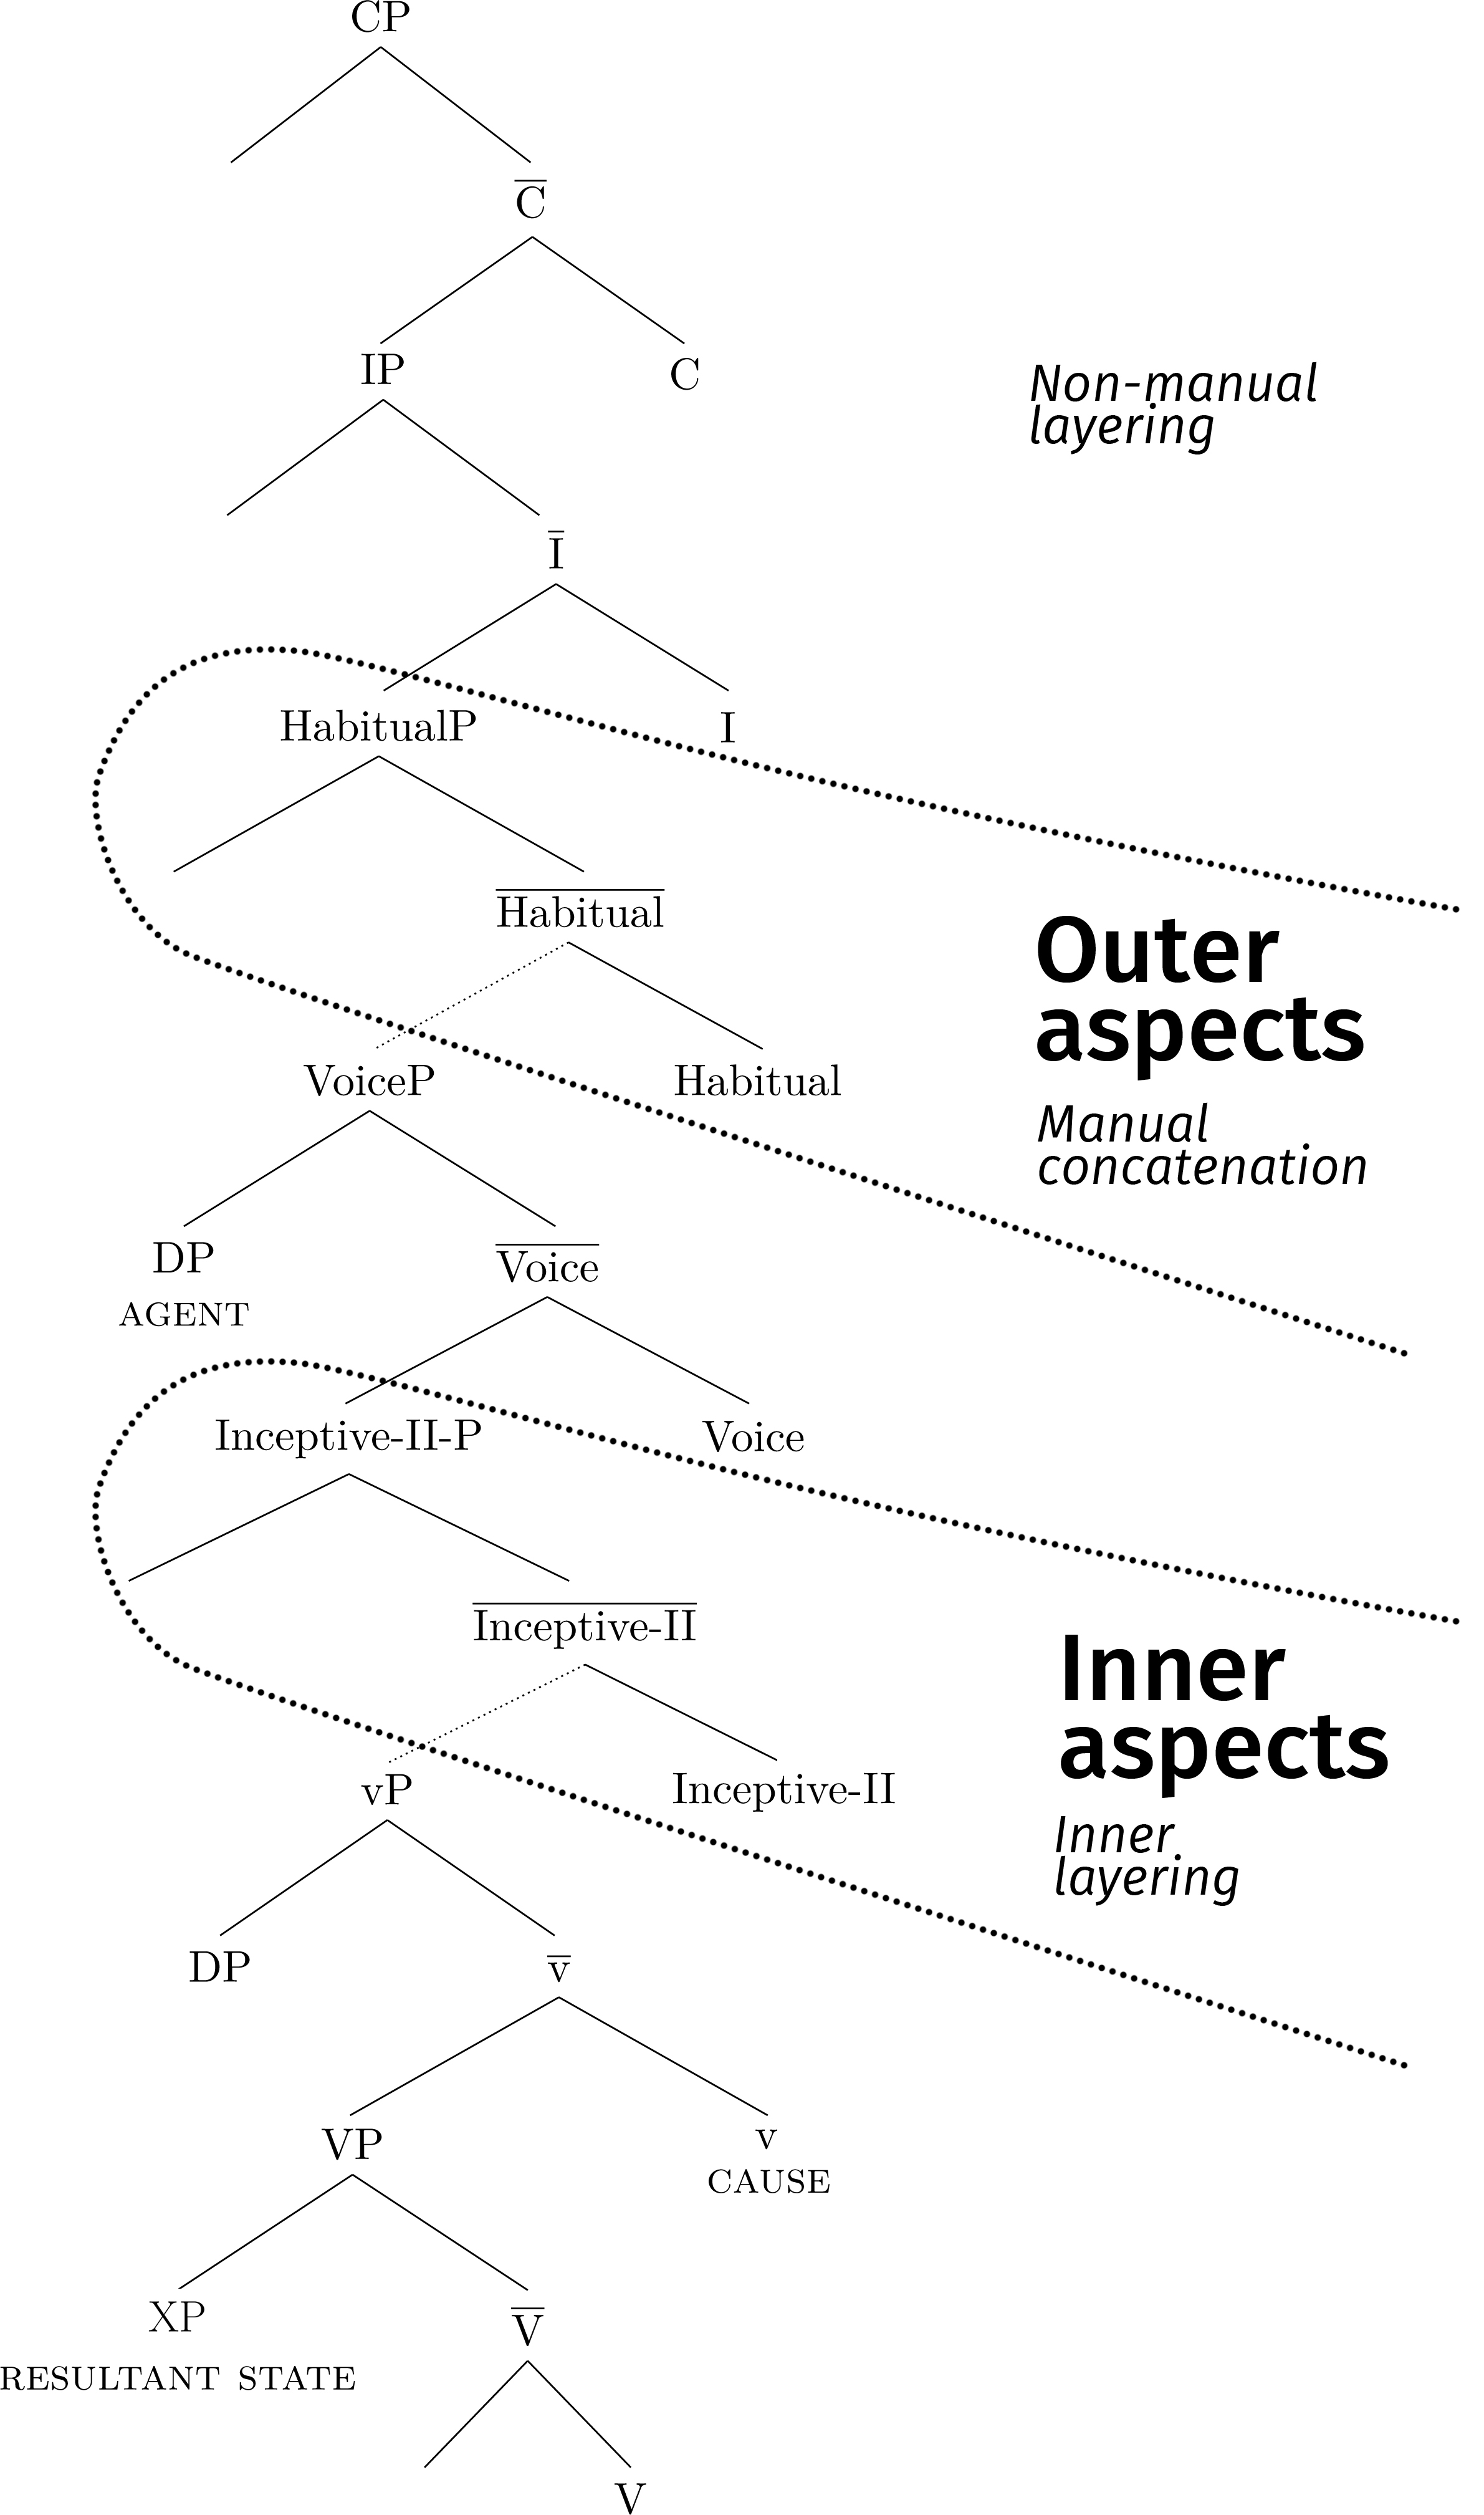
\includegraphics[width=0.88\linewidth]{tree.jpg}%
          }
    \end{minipage}
\end{exe}

%%%%%%The content of chapters/00 can be ignored
\chapter{Theoretical background}\label{chaptertheoreticalbackground}
\section{Introduction}
This book presents an overview of the clause structure of German Sign Language (\textit{Deutsche Geb\"ardensprache}, DGS), an SOV language used in Germany. The main claim is that scopal relations are mapped onto the body in a systematic way in this language, an idea first introduced in \citet{bross2017scope}. I will show that the clausal domains with highest scope, to be more precise all CP functions (i.\,e., all categories above T) are expressed non-manually with the face, starting with the eyebrows and finally switching to the lower face. Lower, IP-internal aspectual categories (called the `outer aspects')\is{outer aspect} are produced manually using adverbs. The same is true for IP-internal modal categories which are expressed using manual modal verb signs. I will show that these manual signs systematically occur pre-verbally, i.\,e., overtly scope from left to right (with the verb being linearly to the right of the scope-taking element). This relation then switches to a right-to-left concatenation strategy when it comes to Voice adverbs (e.\,g., \textsc{well}). Finally, I will show that the lower, VoiceP-internal aspects (called the `inner aspects')\is{aspect}\is{inner aspect} are systematically produced by manipulating the movement path of the verb sign. 

In this first chapter on the theoretical background of the present study, I will introduce the two theoretical frameworks I will follow, namely Generative Grammar (to be more precise Minimalism) and the Cartographic approach to syntax (Section \ref{theoryintroa} and \ref{theoryintrob}). Finally, in Section \ref{hypotheses} the main hypotheses are introduced.% and in Section \ref{methods}, I will discuss data elicitation. Finally, I will give a brief overview of the content of the remainder of the book (Section \ref{outlinesection}).

%\section{Theoretical Underpinnings}\label{theoryintro}


\section{Generative Grammar and the Minimalist Program}\label{theoryintroa}
The goal of the present and the section to follow is to introduce the two theoretical frameworks which underlie the current study. First, I will briefly outline the main claims of the Generative Grammar and the Minimalist program and then, in the next section, discuss the basics of Cartographic syntax. 

Generative Grammar is a grammatical theory in which the grammar of a language is taken to be a set of rules able to create structures (and only those structures) which are judged to be grammatical by native speakers/hearers/signer of that language. While there have been several different approaches or schools in the history of Generative Grammar, what they all have in common is that they try to model the knowledge of an ideal native signer/speaker which allows her/him to master the language. One of these approaches is called `Minimalism' or the `Minimalist program'. Minimalism is a research program in the tradition of Generative Grammar developed in the early 1990s. It is a syntactic account which tries to model syntax in the most parsimonious, natural, and elegant way while not denying that there may be other (equivalent) ways to model syntax. This means that it is more a research program than a theory: ``$[$M$]$inimalism is not a theory so much as a program for research. $[$\dots $]$ Theories are true or false. Programs are fecund or sterile'' \citep[6]{hornstein2005understanding}.

\subsection{Modeling I-language}\is{I-language}
The goal of the Minimalist framework, as with older frameworks in the Generative tradition, is to model the computational system underlying language. As with its predecessors, the Principles and Parameters Theory and Government and Binding, the core goal of the Minimalist program is to study the tacit linguistic competence, i.\,e., the cognitive system which is able to generate grammatical structures, called `I-language'. The I-language, with `I' standing for \textit{internal}, \textit{intensional}, and \textit{individual}, is understood as a property of the mind/brain of an individual, i.\,e., a state of the mind. This state of the mind can have different manifestations. Before a human being has experienced any linguistic input this state is called the `initial state' and after a human being has acquired a language it is called the `steady state' (i.\,e., the state in which an individual has the knowledge to master a language). Thus, Minimalism, as well as its predecessors, tries to study the I-language, an abstract state of the mind, and not (a set of) concrete utterances which are labeled \is{E-language}`E-language', with `E' standing for \textit{externalized} and \textit{extensional} \citep{chomsky1986barr}.

\subsection{The Idea of the Language Faculty and Universal Grammar}
Humans acquire a language through input which means that there is some (limited) data a child has access to, called `primary linguistic data'. The simplest model to account for the fact that humans are able to acquire a language through this input looks like the one in (\ref{simplemodelug}). This model simply states that any typically developing human being is able to acquire any natural language through primary linguistic data as an input. This input is processed by the individual's brain resulting in acquiring competence in the language. 

\begin{exe}
\ex\label{simplemodelug} Primary linguistic data \ding{212} \fbox{human brain} \ding{212} I-language
\end{exe}

\noindent Since the early days of Generative Grammar, the existence of a set of principles for constructing grammars has been postulated, which is thought to be innate in the form of a modular subsystem, while connected to, but crucially encapsulated from, the general cognitive system. The reason for assuming the existence of this system, called `faculty of language' (or `language faculty'), was that humans are able to effortlessly acquire any human language despite its complexity and despite the fact that the primary linguistic data is quite limited and impoverished in nature. From this, the model in (\ref{simplemodelug}) can be reformulated as in (\ref{simplemodelugb}). According to this view, language acquisition ``is primarily a matter of filling in detail within a structure that is innate'' \citep[39]{chomsky1975reflections}.

\begin{exe}
\ex\label{simplemodelugb} Primary linguistic data \ding{212} \fbox{faculty of language} \ding{212} I-language
\end{exe}

\noindent The theory of the initial state of the faculty of language is called `Universal Grammar' (UG), although the term is widely used with the meaning of this state or the module itself. This means that it was assumed that those abstract grammatical principles which are universal should be regarded as being part of our biological endowment, i.\,e., innate. Although there has been much criticism on the idea that this kind of UG exists (e.\,g., \citealt{evans2009myth}; \citealt{levinson2010time}), it is still clear that indeed much uniformity exists across the languages of the world. This does not only relate to the way that languages are acquired, which is cross-linguistically similar, but also to the possible ways grammars are structured. The main controversy since the beginning of Generative syntax has been the origins of this uniformity and the question of whether an innate faculty of language really exists and what it looks like. 
A logical consequence was to reduce the theoretical machinery. Subsequently, the faculty of language was divided into two parts, the language faculty in the broad (FLB) and the language faculty in the narrow sense (FLN) \citep{hauser2002faculty,fitch2005evolution}. While the original idea of Generative approaches was the existence of a linguistic module totally encapsulated from general cognition, it was now thought that the FLB draws back on resources of general cognition and that the FLN only consists of the basic syntactic mechanisms of (recursive) Merge, i.\,e., of an operation that allows structure building and movements. 

This development did not come out of nowhere, but was the result of two competing forces. On the one hand, Generative linguists (following ideas by \citealt{fodor1975language, jerry1983modularity}) have defended the view of a strictly encapsulated language processing module (with several submodules). On the other hand, cognitive psychologists since the 1990s/2000s developed a diametrically opposed view according to which language is not processed in an amodal, encapsulated  module, but processed in brain areas which are highly interrelated with neural circuitries responsible for motor control and perception. Since then, cognitive psychologists have accumulated a huge body of evidence that lends support to the view that linguistic processing draws back on mechanisms of general cognition, a view called `grounded cognition' or `embodied language processing' (see, for example, \citealt{glenberg2002grounding}; \citealt{pecher2005grounding}; \citealt{barsalou2008grounded}).

\begin{figure}[bt]
\centering
	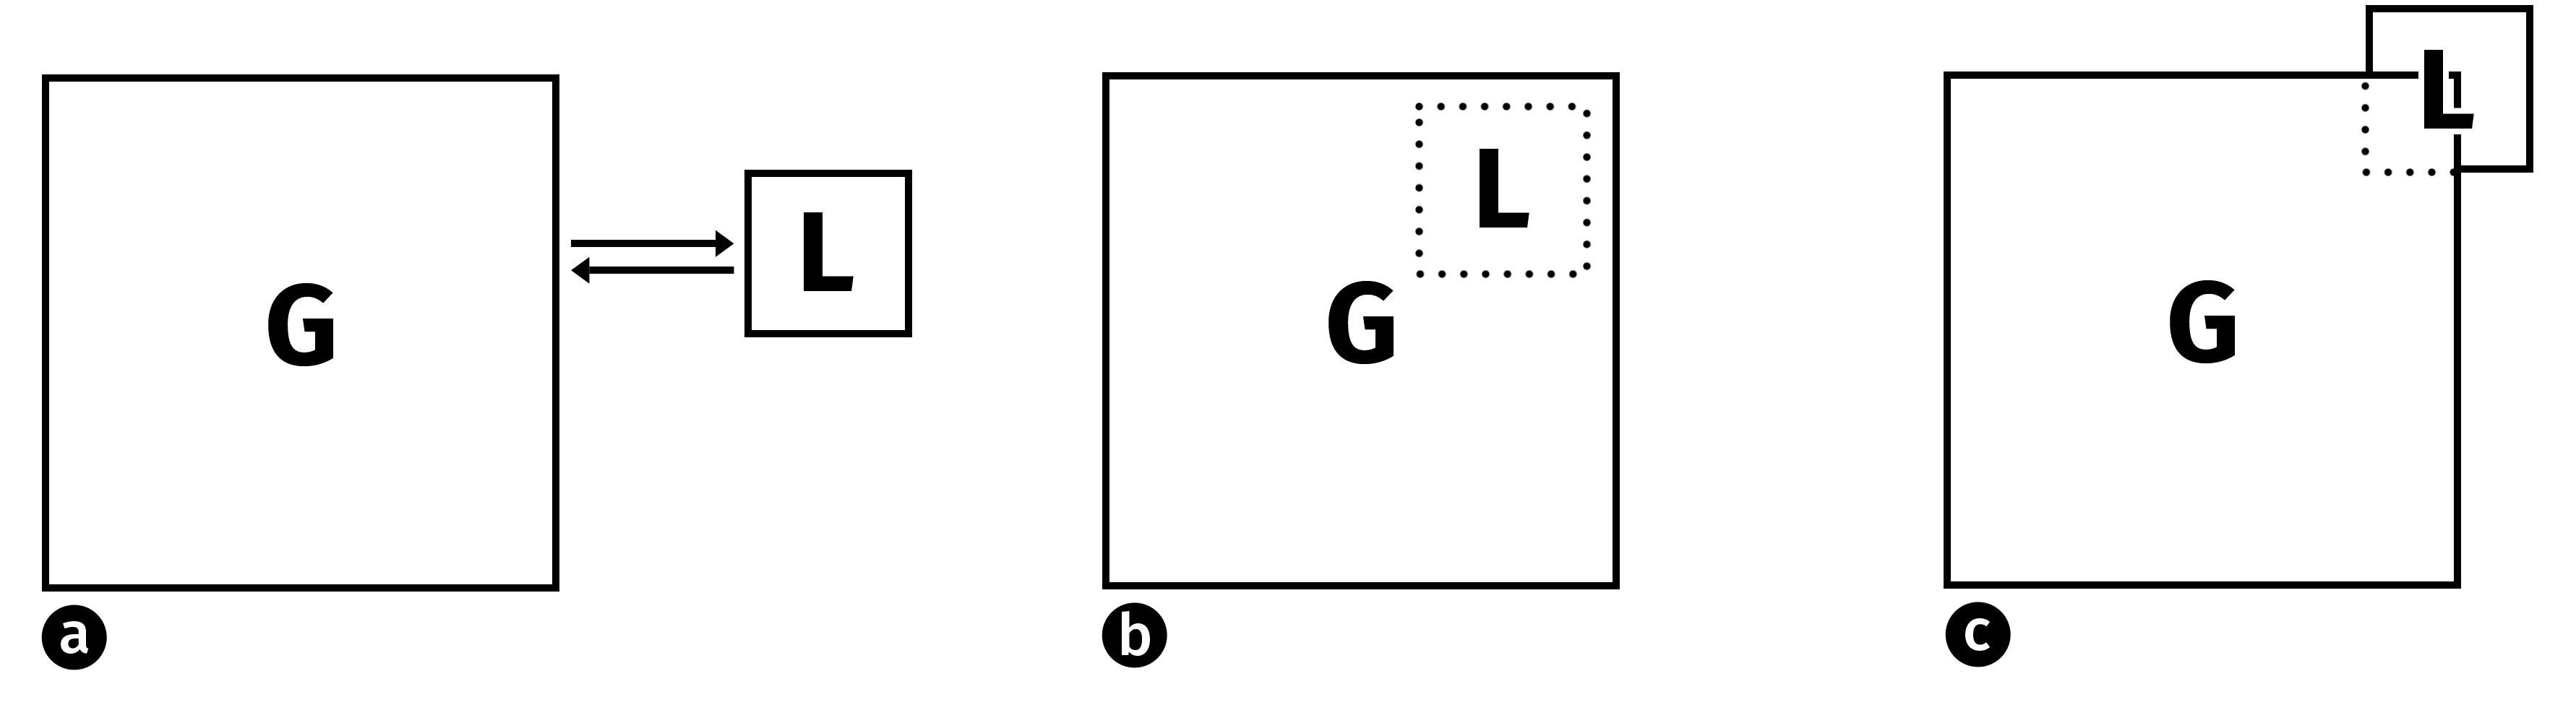
\includegraphics[width=1.0\textwidth]{model.jpg}
	\caption{a) The modular view of language (L) as being an encapsulated and innate module that is separated from general cognition (G); b) Proponents of embodied cognition approaches think of language not as an innate module, but rather as a processing system that draws on general cognitive resources; c) An integrated view.}
	\label{model}
\end{figure}

Thus, according to the modularist view, language is processed in an encapsulated module which is separated by general cognition, as shown in Figure \ref{model}a, while linguistic processing is totally integrated into the general cognition according to embodied language processing approaches, as shown in Figure \ref{model}b.  In a sense, Minimalism is an attempt to bring these two opposing world-views together in claiming that FLN is a separate module and FLB draws back on general cognitive resources, as illustrated in Figure \ref{model}c. This means that both language acquisition and language processing in the adult speaker-hearer/signer rely on two different parts: a specialized language module and general cognition. Thus, while the term `Minimalism' is often understood in a sense that the program tries to minimalize the theoretical machinery used to describe a grammar---and this is indeed true---, the core meaning is that it is not only this machinery that should be minimal, but the language faculty that is modeled as being biologically minimal (e.\,g., \citealt{sigurdsson2011uniformity}).

\subsection{The Y-model of Grammar}
While the basic mechanism of conjoining and manipulating linguistic strings (i.\,e., Merge) is thought of as part of the FLN, there are two systems that play a role in Minimalist approaches being part of general cognition. The first is the sensorimotor system, to be more precise, the articulatory-perceptual system (A-P system) and the second the conceptual-intentional system (C-I system). As these systems need to communicate with the modules responsible for linguistic processing, there is a need for at least two interfaces. These interfaces, i.\,e., the linguistic levels connected to the A-P system and the C-I system respectively, are the Phonological Form (PF) and the Logical Form (LF). While PF is the mental representation of sound/sign, LF is the mental representation of meaning, although in a rather abstract sense as LF is only concerned with the part of meaning which can be derived from structural relationships (in a syntactic tree).
 
\begin{figure}[bt]
\centering
	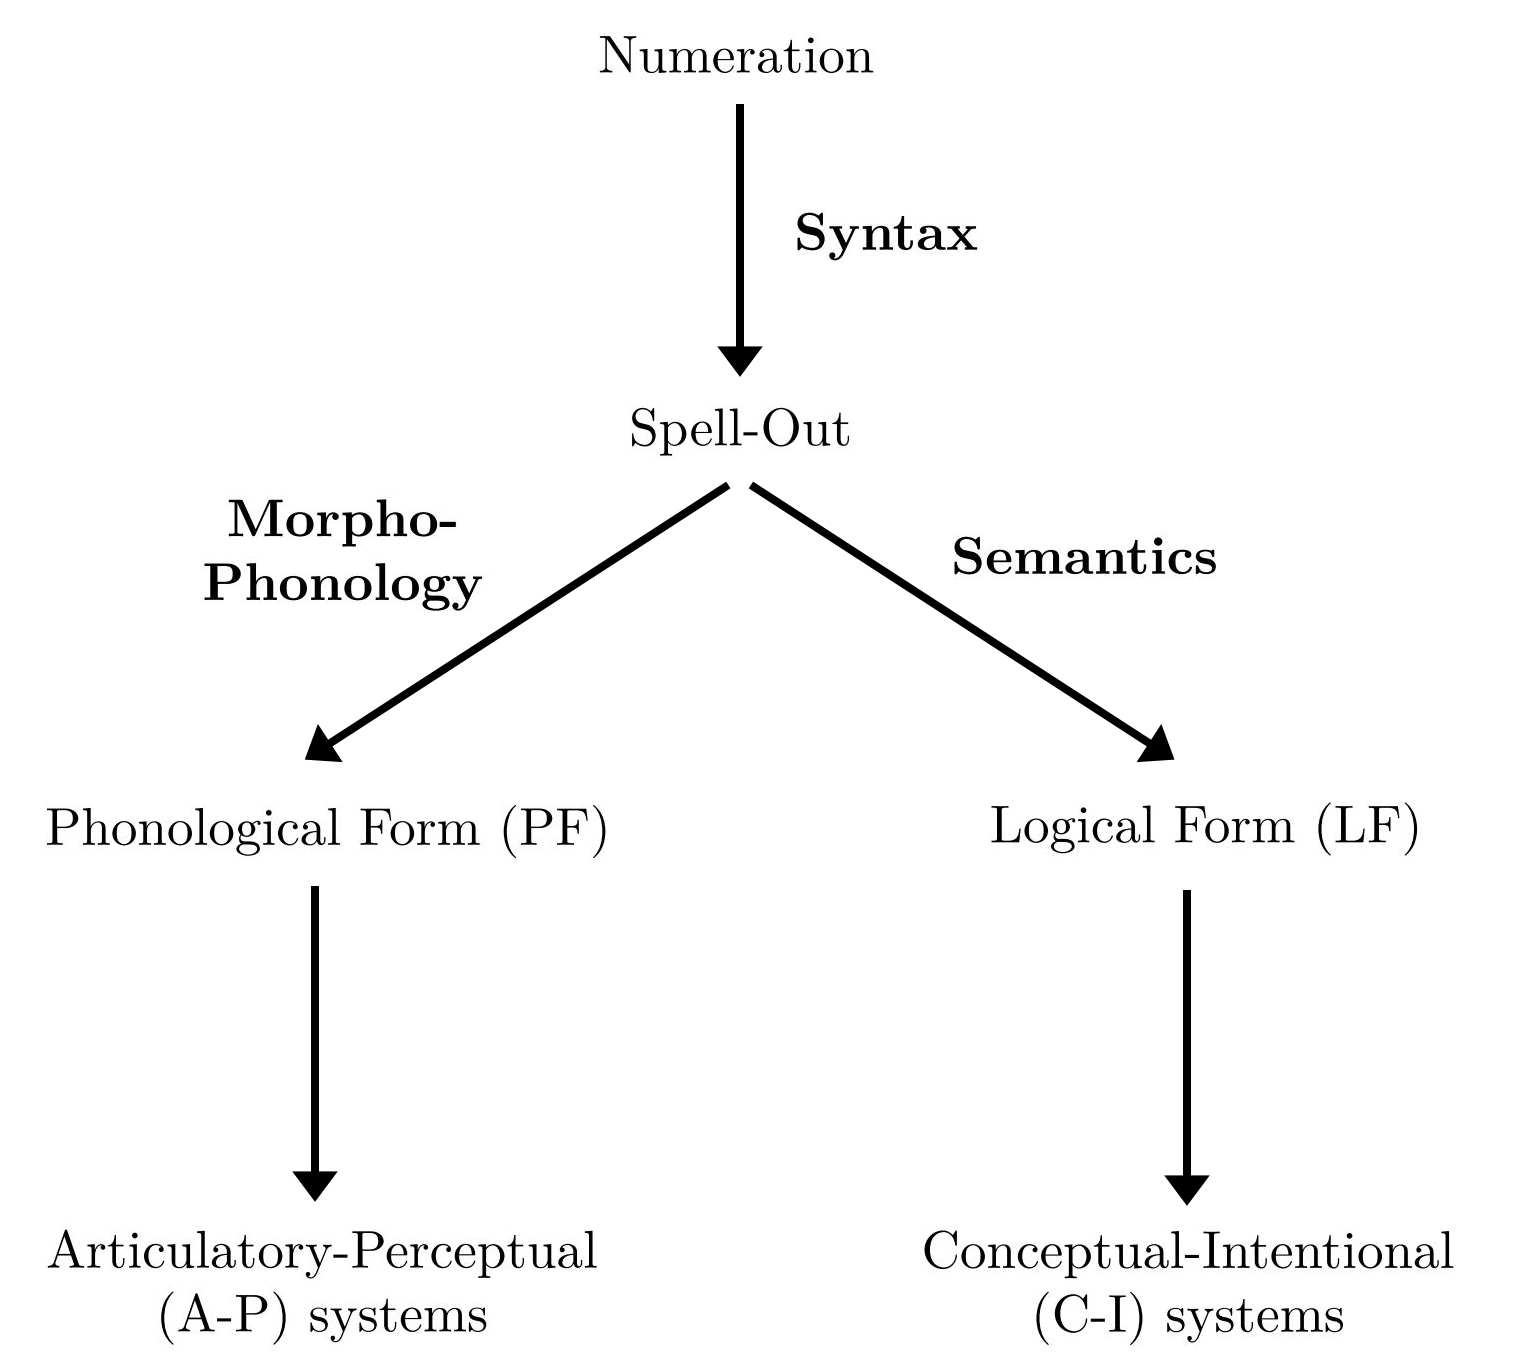
\includegraphics[width=1.0\textwidth]{ymodel.jpg}
	\caption{The Y-model of grammar.}
	\label{ymodel}
\end{figure}

The relation between PF and LF (as the interfaces) on the one hand and the A-P and the C-I system on the other are depicted in what is generally known as the `Y-model of grammar' (also called `T-model of grammar'), shown in Figure \ref{ymodel}. The basic idea of this model is that the derivation of a sentence starts by picking out the lexical items needed to construct a sentence (note that the term `lexical item' is used in a very broad sense here as it includes both content and functional elements). This string of lexical items is called the `numeration'. The numeration is handed over into what is called the `workspace of the derivation'. In the workspace, syntactic operations are performed on the numeration, i.\,e., syntactic structure is built via two types of Merge: External Merge combines two elements and Internal Merge (also Remerge or Movement) operates on syntactic objects created via External Merge. This module, labeled `syntax' in the Y-model in Figure \ref{ymodel}, is sometimes called `overt syntax' as the operations carried out in this module produce audible/visible effects in the syntax.

At this point in the derivation, i.\,e., after syntax has produced a syntactic object via External and Internal Merge, the syntactic object is shipped off to the interfaces. This point in the derivation is called `Spell-Out' (note that this is not the point at which something is actually pronounced as the name may suggest). Here, the derivation splits up, as there are syntactic operations which are not visible when pronouncing or signing a sentence. Think of \textit{wh}-\textit{in-situ}-languages in which a \textit{wh}-operator is interpreted as if it were high up in the structure although this is not the case in the actual sentence. To account for this, a module is needed to take care of such operations. This module is labeled `semantics' in Figure \ref{ymodel}. Sometimes this module is also called `covert syntax' as the operations carried out in the module are not overt. Note, again, that semantics or meaning at this point of the derivation only refers to meaning which can be derived from structural relationships (which does, of course, not mean that elements from the derivation having meaning on their own cannot enter this branch). As what is actually pronounced or signed can be different from the LF representation, another branch is needed in which morphological and phonological operations can be carried out. The results of these operations are shipped to the PF interface, as shown in the figure.

\subsection{Features}

The most concrete entity in a derivation as has been sketched so far is a lexical item and the most concrete form of a lexical item is a word. Each word in a language follows it own rules. There is a rule for how to pronounce it, a rule for what the word means, and rules for what the morphological shape of a word looks like in certain environments. These `rules' are called features. Thus, a lexical item consists (at most) of phonological, semantic, and morphosyntactic features---note that this leaves open the possibility that lexical items without phonological features exist. If we look at morphosyntactic features, it turns out that they come in two flavors. Some features have semantic content and others do not. Take the word \textit{cats} which bears a plural feature (the plural marker /z/ is not the feature itself, but the realization of this feature). This feature has semantic import as it becomes clear that a word like \textit{cats} is referring to several entities. Features of this type are called `interpretable features' as they are interpretable at LF. The terminological counterpart of interpretable features are uninterpretable features which, then, are features which are not interpretable at LF. An example of an uninterpretable feature is Case: In the example in (\ref{casea}), the pronoun \textit{her} is, because of its syntactic position, required to be in objective case. This particular construction does not allow another Case. Nominative Case, for example, is disallowed, as shown in (\ref{caseb}). This is a pure structural requirement and does not directly add anything to the meaning as we can see from the example in (\ref{casec}) which are equal from a semantic perspective, but in this structure only nominative Case is allowed (cf. (\ref{cased})). 

\begin{exe}
\ex\label{case}\begin{xlist}
\ex \textcolor{white}{*}G\"okce believes \textit{her} to be smart. \label{casea}
\ex *G\"okce believes \textit{she} to be smart. \label{caseb}
\ex \textcolor{white}{*}G\"okce believes that \textit{she} is smart. \label{casec}
\ex *G\"okce believes that \textit{her} is smart. \label{cased}
\end{xlist}
\end{exe}








\noindent Lexical items are not only specified for features by themselves, but also bear features specifying what features other lexical items should carry in order to be able to Merge with them. Such features are called subcategorization features. Take the lexical item \textit{to} in a construction like \textit{I gave the beer to Felicia} which can, obviously, be Merged with a DP (in this case, the DP \textit{Felicia}). We can thus state that the preposition \textit{to} has an uninterpretable subcategorization feature $[$\textit{u}DP$]$. As the DP \textit{Felicia} bears a matching feature, the features are checked (or valuated) in the derivation and subsequently deleted. The deletion of uninterpretable features is necessary as the derivation would crash if features which are not interpretable at LF enter LF or PF. From this, it becomes clear that features are the driving force of Merge. This is true not only for External Merge, but also for Internal Merge. Thus movement (or Internal Merge) must be motivated in some way and this way is feature checking (or: feature valuation). 

\subsection{The $\overline{\textrm{X}}$ Schema}
\is{x schema@$\overline{\textrm{X}}$ schema|(}
As External Merge always combines two lexical items (or more broadly speaking, two syntactic objects) it is an operation which always leads to binary branching structures \citep{kaynel984}. As (External) Merge has been, so far, only defined as an operation which takes two syntactic objects and combines them into a larger syntactic object, Merge is an extremely powerful mechanism which needs to be constrained in order to not overgeneralize. A first constraint on Merge was already introduced with subcategorization features. Another constraint concerns the way the resulting structures look. The way the output (i.\,e., phrases) looks is modeled by the $\overline{\textrm{X}}$ schema (`X-bar schema') which states that all phrases have essentially the same structural skeleton \citep{jackendoff1977x,chomsky1986barr}:\footnote{ Note that some frameworks try to get rid of the $\overline{\textrm{X}}$ schema completely by assuming that all levels of the $\overline{\textrm{X}}$ structure can be read off from structural relationships of the tree geometry created by merge (e.\,g., \citealt{chomsky1995bare}). However, I will not adopt such a bare phrase structure approach\is{bare phrase structure} as the Cartographic framework I am working in traditionally models clausal maps in an $\overline{\textrm{X}}$ format, but nothing hinges on that as I assume that $\overline{\textrm{X}}$ structures and bare phrase structures are compatible and that one representation can be translated into the other.} Phrases are organized around syntactic heads which determine the categorical status of a phrase. Heads may optionally have sisters which themselves are phrases. These sisters are called `complements'. Additionally, heads may have an immediately c-commanding phrase called `specifier' with c-command (constituent command), informally being defined as having a structural relationship of the following form: a node A in a syntactic tree c-commands its sister B and all the descendants of B, i.\,e., all nodes dominated by B. We thus arrive at a structural representation as in (\ref{xbar}). 

\begin{exe}
\ex\label{xbar} 
\begin{tikzpicture}[baseline={([yshift={-2.3ex}]current bounding box.north)}, scale=0.90]
\tikzset{level distance=50pt,sibling distance=25pt,every tree node/.style={align=center,anchor=north}}
\Tree [.XP [.SpecXP ] [.{$\overline{\text{X}}$} [.{X\textdegree } ] [.{YP (Complement)} ] ] ] 
\end{tikzpicture}
\end{exe}

\noindent The representation in (\ref{xbar}) tells us that the core of the $\overline{\textrm{X}}$ schema is a head, in this case the head X\textdegree\ (with the little circle being an abbreviation for head). It projects its categorical status to the whole phrase which then is an XP. While there may be more structure built around an XP, the categorical status cannot project any further. For this reason, XPs are also called `maximal projections'. Note that the terms `specifier', `head', and `complement' are purely structural terms which means that it does not matter on which side of the tree any of the three elements are located. Thus, the structure in (\ref{xbarb}) is also in accordance with the $\overline{\textrm{X}}$ schema (as would be structures with a specifier on one and the head on the other side of the tree).

\begin{exe}
\ex\label{xbarb} 
\begin{tikzpicture}[baseline={([yshift={-2.3ex}]current bounding box.north)}, scale=0.90]
\tikzset{level distance=50pt,sibling distance=25pt,every tree node/.style={align=center,anchor=north}}
\Tree [.XP [.{$\overline{\text{X}}$} [.{YP (Complement)} ] [.{X\textdegree } ] ] [.SpecXP ] ] 
\end{tikzpicture}
\end{exe}

\noindent However, in a particular version of the $\overline{\textrm{X}}$ theory, called `Antisymmety' \citep{kayne1994antisymmetry}, only specifier-head-complement orders are allowed which means that phrases always have a make-up as in (\ref{xbar}), i.\,e., in this framework all specifiers are left-branching and all heads are left-headed. Thus, according to Antisymmetry, all deviations from a specifier-head-complement order are derived via Remerge (movement) operations. 

It is assumed that all heads project phrases in accordance with the $\overline{\textrm{X}}$ schema. This means that not only lexical categories, such as nouns (projecting an NP) or verbs (projecting a VP) are in line with the $\overline{\textrm{X}}$ schema, but also functional categories like tense (projecting a TP or IP for `inflectional phrase'), determiners (projecting a DP), or complementizers (projecting a CP). 
\is{x schema@$\overline{\textrm{X}}$ schema|)}
\subsection{Adjunction}\label{generaladjunction}
\is{Chomsky-adjunction|see{adjunction}}
\is{adjunction|(}
The final operation I want to briefly introduce is adjunction (Chomsky-adjunction). This is an operation which tries to capture the fact that not all lexical items in a syntactic structure can be accounted for by \is{subcategorization feature}subcategorization features of heads or feature checking. Adjuncts are traditionally viewed as being sisters of maximal projections being themselves also maximal projections---although on some accounts head adjunction, i.\,e., adjunction to intermediate projections is also allowed. Adjuncts are often introduced by contrasting them with arguments of the verb. Let's take a simple example such as the sentence in (\ref{simpleargumentsoftheverb}). The verb \textit{to drink} takes two arguments, in this case the DPs \textit{Julian} and \textit{a beer}. The arguments of the verb are required by the verb because of its subcategorizitation features. This means that the sentence would be either ill-formed if an argument is left out (*\textit{drinks a beer}) or the sentence is well-formed but does still entail the same relation between the verb and the omitted argument (\textit{Julian drinks} entails that Julian drinks something) (see \citealt{hole2015arguments}).

\begin{exe}
\ex\label{simpleargumentsoftheverb} Julian drinks a beer.
\end{exe}

\noindent This is different with adjuncts. We can easily add adjuncts to the sentence in (\ref{simpleargumentsoftheverb}), as in (\ref{simpleargumentsoftheverbb}). In this example, I added the two PP adjuncts \textit{on Sunday} and \textit{in the beer garden}. However, the sentence would still be grammatical if I left one or both out (this is evidenced by (\ref{simpleargumentsoftheverb})). 

\begin{exe}
\ex\label{simpleargumentsoftheverbb} Julian drinks a beer $[$on Sunday$]$ $[$in the beer garden$]$.
\end{exe}

\noindent As adjunction simply means expanding a category XP by adjoining another XP it does not matter in which order adjunction takes place, as shown in (\ref{simpleargumentsoftheverbbb})

\begin{exe}
\ex\label{simpleargumentsoftheverbbb} Julian drinks a beer $[$in the beer garden$]$ $[$on Sunday$]$.
\end{exe}

\noindent Traditionally, it is not only PPs specifying the place or time an event took place that are modeled as adjuncts, but also adverb and adjective phrases, as adverbs and adjectives are not required by any subcategorization features.  However, the question whether adjunction really exists is highly controversial, as will be discussed in the following section.
\label{generaladjunctionb}

\is{adjunction|)}

\section{Cartography---A Mendeleev Table for Syntax}\label{cartographicenterprise}\label{theoryintrob}
\subsection{General Overview}
Roughly at the same time Minimalism was developed, the development of the Cartographic research program began. While Minimalism concentrates on the syntactic computations involved in structure building, Cartography is concerned with the fine-grained details of these structures (e.\,g., \citealt{cinque1999adverbs}; \citealt{rizzi2004cartography}; \citealt{belletti2008structures}; \citealt{cinque2008cartography}). The goal of Cartographic syntax is to draw a precise map of all portions of the syntactic structure of the clause. One main requirement of such maps is that they should hold cross-linguistically, i.\,e., the goal is to find the universal functional structures underlying all languages. 

The main assumption of Cartographic approaches to syntax is, of course, that such a fixed set of functional projections exists. One problem related to figuring out which projections indeed exist is that they can find different expressions in different languages (e.\,g., as heads in the form of affixes or particles or as XP-adverbials)---or even no grammaticalized expression at all. This can be illustrated for the category of \is{evidentiality}evidentiality. Many languages have verbal affixes to express the kind of evidence the speaker/signer has concerning her/his statement. In \is{West Greenlandic}West Greenlandic, for example, a speaker might encode that s/he has direct, visual evidence or indirect hearsay evidence of something expressed by the verb \citep{fortescue2003evidentiality}. To indicate visual evidence, the affix \textit{-(r)paluC-} is used and to indicate hearsay evidence, the affix \textit{-(r)pallaC-} is used. This is illustrated in (\ref{ex:westgreenlandicevidential}) and (\ref{ex:westgreenlandicevidentialb}).

\begin{exe}
\ex West Greenlandic \citep[294--295]{fortescue2003evidentiality} \begin{xlist}
\ex \gll {\textit{napparsima-rpalup-puq}} \\
{be.ill-(r)paluC-\textsc{3sg}+\textsc{indic}} \\
\trans `He looks ill.' \label{ex:westgreenlandicevidential}

\ex \gll {\textit{angir-pallap-puq}} \\
{say.yes-(r)pallaC-\textsc{3sg}+\textsc{indic}} \\
\trans `He is supposed to have said yes (I have heard).' \label{ex:westgreenlandicevidentialb}

\end{xlist}
\end{exe} 

\noindent Other languages express the same categories in different ways. In \is{German}German, for example, direct visual evidence can be expressed by using the verb \textit{wirken} `to appear', hearsay evidence by the modal verb \textit{sollen} `should'. Thus, while West Greenlandinc uses affixes, German express the same contrast by using different verbs.  This is shown in the examples in (\ref{ex:germanevidentialsystema}) and (\ref{ex:germanevidentialsystemb}). 

\begin{exe}
\ex German\begin{xlist}
\ex \gll {\textit{Er}} {\textit{wirkt}} {\textit{krank.}} \\
{he} {appears} {sick} \\
\trans `He looks ill.' \label{ex:germanevidentialsystema}
\ex \gll {\textit{Er}} {\textit{soll}} {\textit{ja}} {\textit{gesagt}} {\textit{haben}} \\
{he} {should} {yes} {said} {have} \\
\trans `He is supposed to have said yes (I have heard).' \label{ex:germanevidentialsystemb}
\end{xlist}
\end{exe} 

\noindent Yet other languages might have no grammaticalized way to express a category. This can be exemplified for \is{English}English which lacks a grammaticalized form to express hearsay evidence (which does not mean that there are no other ways to express this category). 

Taken together, it is assumed that a fixed set of functional projections exists, but that there is cross-linguistic variation as to if and how a language expresses these features (see already \citealt{vergnaud1985dependances}). Thus, while the order of the projections is taken to be cross-linguistically fixed, variation stems from the choice of a language if a category is to be expressed at all. If it is overtly expressed, variation is thought to stem from the choice of how it is to be expressed---either by an element with head status (e.\,g., a particle or an affix) or an element with phrasal status (e.\,g., an adverb). Additionally, according to some variants of Cartography, it is possible that a language lumps together several categories into one syntactic head. Accounts of this type, sometimes called `Cartography light' \citep{van2009alternatives}, are found, for example, in \citet{rizzi1996residual}, \citet{thrainsson1996non}, or \citet{bobaljik1998two}.

\subsection{The Cartographic Method---Exemplified by Adjective Ordering Restrictions}

\is{adjective ordering restrictions|(}
Adjective ordering restrictions are a good starting point to illustrate how syntactic Cartographers proceed to investigate the functional make-up of syntactic structures. It is a well-known fact that adjectives modifying nouns exhibit cross-linguistically stable ordering restrictions (see already \citealt{whorf1945grammatical}). In \is{English}English, for example, we find that evaluative adjectives precede size adjectives, as shown in (\ref{ex:brownbeautifula}). Although it is in principle possible to switch the order of evaluative and size adjectives (\ref{ex:brownbeautifulb}), this order is clearly marked by a special intonation, for example, comma intonation or focus would be required \citep{sproat1991cross} to produce (\ref{ex:brownbeautifulb}) in a naturally sounding way. Thus, the order in (\ref{ex:brownbeautifula}) is taken to be the neutral order---also because no special discourse context is required to produce this order.

\begin{exe}
\ex\label{brownbeautiful}\begin{xlist} 
\ex \textcolor{white}{\#}{a cute tiny kitten\label{ex:brownbeautifula} }
\ex \#{a tiny cute kitten \label{ex:brownbeautifulb}}
\end{xlist}
\end{exe}

\noindent The generalization of the order of evaluative and size adjectives is not a generalization of individual adjectives, but of whole categories. This means that the generalization does not only hold for \textit{cute} and \textit{tiny}, but for the whole class of evaluative adjectives (e.\,g., \textit{beautiful}, \textit{ugly}, etc.) and the whole class of size adjectives (e.\,g., \textit{small}, \textit{huge}, etc.). Additionally, we find similar constraints for other adjective classes. 
\is{transitivity (method)|(}
It is, in principle, possible to have an infinite number of adjectives modifying a noun, such as (\textit{I bought these}) \textit{three beautiful huge long brown rugs}. However, processing and memory limitations put constraints on the number of adjectives that can be used. Instead of building large phrases as the one just mentioned it makes more sense to use a more systematic way of figuring out adjective ordering restrictions. The method commonly used is based on transitivity. This means that we first take a pair A and B and look at their ordering restrictions. Then we will look at a pair B and C. From the ordering of this pair a prediction of the ordering of A and C can be (transitively) inferred: ``if A must occur on B's left, and B must appear on C's left, we can infer that A will appear to the left of C and test it as a prediction of our theory. It is possible to construct a theoretical sequence of positions, A, B, C, etc., even if the three never appear together'' \citep[42]{beninca2001position}.


By now, we have figured out that, in \is{English}English, evaluative adjectives precede size adjectives. We now can test, for example, what happens with color adjectives like \textit{black}. If we combine a color adjective with a size adjective, we find that size adjectives precede color adjectives, as shown in (\ref{brownbeautifulbccc}).

\begin{exe}
\ex\label{brownbeautifulbccc}\begin{xlist} 
\ex \textcolor{white}{\#}a small black cat \label{ex:brownbeautifulba} 
\ex \#{a black small cat \label{ex:brownbeautifulbb} }
\end{xlist}
\end{exe}

\noindent We now can start building a hierarchy. We have figured out that evaluative adjectives precede size adjectives (\ref{firsthierarchya}) and that size adjectives precede color adjectives (\ref{firsthierarchyb}). Combining these insights, following the transitivity logic, we can make the prediction in (\ref{firsthierarchyc}). This prediction can be tested empirically. If it turns out to be true, we arrive at the ordering in (\ref{firsthierarchyd}).


\begin{exe}
\ex\label{firsthierarchy}\begin{xlist} 
\ex evaluative adjectives $>$ size adjectives \hfill A $>$ B \label{firsthierarchya}
\ex size adjectives $>$ color adjectives \hfill B $>$ C \label{firsthierarchyb} 
\ex evaluative adjectives $>$ color adjectives \hfill A $>$ C \label{firsthierarchyc}
\ex eval. adjectives $>$ size adjectives $>$ color adjectives \hfill A $>$ B $>$ C \label{firsthierarchyd}
\end{xlist}
\end{exe}


\noindent The hypothesis in (\ref{firsthierarchyc}) indeed turns out to be on the right track, as illustrated in (\ref{brownbeautifulbb}). Thus, the hierarchy in (\ref{firsthierarchyd}) is correct.

\begin{exe}
\ex\label{brownbeautifulbb}\begin{xlist} 
\ex \textcolor{white}{\#}a cute black cat \label{ex:brownbeautifulbba} 
\ex \#{a black cute cat \label{ex:brownbeautifulbbb} }
\end{xlist}
\end{exe}

\noindent By using the empirical method of transitivity testing, we arrive at the ordering restrictions in (\ref{aorestra}) (cf. \citealt{kingsbury1986longman}; \citealt{sproat1991cross}; \citealt{cinque1994evidence}; \citealt[1304--1308]{hole2015arguments}; \citealt[107--110]{van2017syntax}). Note that the ordering presented here is only an example and that it would be no problem to derive even more fine-grained orderings.

\begin{exe}
\ex\label{aorestra} (Determiner $>$ Number $>$) Evaluation $>$ Size $>$ Age $>$ Shape $>$ Color $>$ Origin $>$ Material ($>$ Noun)
\end{exe}

\noindent As can be seen from this hierarchy, we are in fact dealing with a structure that is located between a determiner and a noun, i.\,e., the internal structure of the DP. We now have to ask how to model these findings syntactically. In a traditional analysis, this would be modeled via adjunction. This means that the adjectives would simply be adjoined to the NP, as depicted in (\ref{ex:kittenadjunctiontree}) or, alternatively, by adjunction to intermediate projections, as shown in (\ref{ex:kittenadjunctiontreeb}).

\begin{exe}
\ex
\begin{multicols}{2}
\begin{xlist}
\ex \label{ex:kittenadjunctiontree}
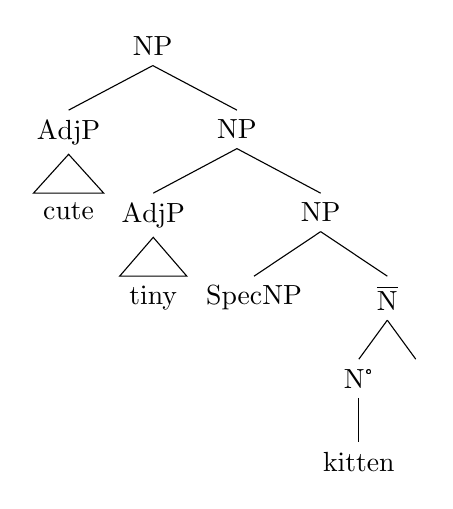
\begin{tikzpicture}[baseline=(current bounding box.north), scale=1.00]
\tikzset{sibling distance=1pt}
\tikzset{every tree node/.style={align=left,anchor=north}}
\Tree [.NP [.{AdjP} \edge[roof];  \node(labelone){cute}; ] [.NP [.{AdjP} \edge[roof];  \node(labeltwo){tiny}; ] [.NP [.SpecNP ] [.{$\overline{\textrm{N}}$} [.{N\textdegree} kitten ] [.{} ] ] ] ] ]
\end{tikzpicture}

\ex \label{ex:kittenadjunctiontreeb}
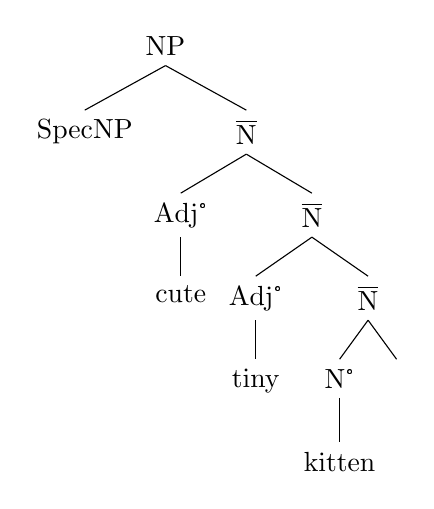
\begin{tikzpicture}[baseline=(current bounding box.north), scale=1.00]
\tikzset{sibling distance=1pt}
\tikzset{every tree node/.style={align=left,anchor=north}}
\Tree [.NP [.SpecNP ] [.{$\overline{\textrm{N}}$} [.{Adj\textdegree } cute ] [.{$\overline{\textrm{N}}$} [.{Adj\textdegree } tiny ] [.{$\overline{\textrm{N}}$} [.{N\textdegree} kitten ] [.{} ] ] ] ] ]
\end{tikzpicture}


\end{xlist}
\end{multicols}
\end{exe}





\noindent We can immediately rule out the approach in (\ref{ex:kittenadjunctiontreeb}), as it can be shown that adjectives should be regarded as phrases and not as heads as it is possible to replace an adjective with a multi-word expression. For example, it is possible to replace \textit{cute} in \textit{a cute kitten} by \textit{extremely cute} resulting in \textit{an extremely cute kitten}. Additionally, the intermediate-projection adjunction approach is theoretically hard to motivate as ``no other category allows recursive adjunction to an intermediate projection'' \citep[94]{scott2002stacked}. This would lead us to assume that NPs are, in terms of $\overline{\textrm{N}}$ structure, unique---an undesirable result (see also \citealt{abney1987english}). This leaves us with the possibility in (\ref{ex:kittenadjunctiontree}). However, there is a major problem which, in fact, also occurs with the structure in (\ref{ex:kittenadjunctiontreeb}): adjunction should be free. This means that the order of the adjuncts should play no role (as already argued on page \pageref{generaladjunction}).

So far, we have seen that English exhibits a strict ordering of adjective phrases inside the DP---a result which is simply an empirical generalization and can hardly be denied. Additionally, it seems as if an adjunction approach is not capable of explaining these restrictions as it would predict the order to be absent. It is thus plausible to assume a rigidly ordered set of (functional) projections as exemplarily shown for the DP \textit{these three beautiful huge old round brown rugs} in (\ref{ex:adjectivetree}). Note that a structure like the one in (\ref{ex:adjectivetree}) simply states that the adjectives are rigidly ordered and says nothing about why this order exists. 




\begin{exe}
\ex \label{ex:adjectivetree}
%\begin{tikzpicture}[baseline=(current bounding box.north), scale=1.00]
%\tikzset{sibling distance=5pt}
\begin{adjustbox}{max width=0.9\textwidth}
\begin{tikzpicture}[baseline=(current bounding box.north),sibling distance=2pt,level distance=45pt
]
%\tikzset{sibling distance=2pt}
\tikzset{every tree node/.style={align=left,anchor=north}}
\Tree [.{{\large DP}} [.{{\large SpecDP}} ] [.{\large{$\overline{\textrm{D}}$}} [.{\large{{D\textdegree}}} {\large{These}} ] [.{\large{NumP}} [.{\large{AdvP}} \edge[roof];  \node(three){{\large{three}}}; ] [.{\large{{$\overline{\textrm{Num}}$}}} [.{\large{{Num\textdegree}}} ] [.{\large{EvalP}} [.{\large{AdvP}} \edge[roof];  \node(beautiful){{\large{beautiful}}}; ] [.{\large{{$\overline{\textrm{Eval}}$}}} [.{\large{{Eval\textdegree}}} ] [.{\large{SizeP}} [.{\large{AdvP}} \edge[roof];  \node(huge){{\large{huge}}}; ] [.{\large{{$\overline{\textrm{Size}}$}}} [.{\large{{Size\textdegree}}} ] [.{\large{AgeP}} [.{\large{AdvP}} \edge[roof];  \node(old){{\large{old}}}; ] [.{\large{{$\overline{\textrm{Age}}$}}} [.{\large{{Age\textdegree}}} ] [.{\large{ShapeP}} [.{\large{SpecShapeP}} \edge[roof];  \node(round){{\large{round}}}; ] [.{\large{{$\overline{\textrm{Shape}}$}}} [.{\large{{Shape\textdegree}}} ] [.{\large{ColorP}} [.{\large{AdvP}} \edge[roof];  \node(brown){{\large{brown}}};  ] [.{\large{{$\overline{\textrm{Color}}$}}} [.{\large{{Color\textdegree}}} ] [.{\large{NP}} \edge[roof]; \node(kaffee){{\large{rugs}}}; ] ] ] ] ] ] ] ] ] ] ] ] ] ] ]

\end{tikzpicture}
\end{adjustbox}
\end{exe}

\noindent According to the Cartographic view, i.\,e., on the assumption that, for example, adjectives are ordered in a fixed set of functional projections, as in (\ref{ex:adjectivetree}), the meaning of the adjectives does not only come from their lexical entries, but is also a function of their syntactic position. What this means is that specific adjective classes (such as evaluative adjectives or size adjectives) are licensed by dedicated functional heads. One interesting piece of evidence that this hypothesis is on the right track is that it is possible for an adjective to receive different interpretations in different positions. This can be illustrated for adjectives which have several readings. An example of such an adjective is \textit{cool} which has a reading as an evaluative adjective meaning `excellent' and a reading as a temperature adjective meaning `not hot' \citep{scott2002stacked}. Although the hierarchies above did not include a TempP so far, we can assume that evaluative adjectives are rather high and temperature adjectives are rather low in the structure---this is because subjective evaluations seem, in general, to be located rather high in the structure and merely descriptive assesements, such as form, color, or temperature, are located nearer to the noun. This leads us to assume that the adjective \textit{cool} can occupy both positions. And indeed, as \citep[106]{scott2002stacked} illustrates, it is easy to construct examples for both positions as shown in (\ref{coolevaltemp}). Note that the adjective under discussion is in an unexpected position in both examples. 

\begin{exe}
\ex\label{coolevaltemp}\begin{xlist} 
\ex What a long cool red dress. \label{coolevaltempa}
\ex What a cool long red drink. \label{coolevaltempb}
\end{xlist}
\end{exe}

\noindent When putting \textit{cool} in a lower position, as in (\ref{coolevaltempa}), we get the somehow strange reading that the dress that is talked about is not hot, in the sense of cold, i.\,e., a temperature reading.\footnote{ Note that the sentence in (\ref{coolevaltempa}) can additionally be a case in which \textit{long} is preposed by focus movement. However, this is not the kind of structure I am aiming here at.} The sentence, however, does not mean that the dress is excellent. In (\ref{coolevaltempb}), it is the other way around. The adjective is in a high position leading to a reading where \textit{cool} does not refer to the temperature, but to the evaluation of the drink being excellent. Additional support of the idea that different positions license different readings comes from the fact that both readings can be combined, as in \textit{a cool cool drink}.\footnote{ Although such constructions are not widely used due to a general constraint that disfavors phonological similar elements to be adjacent, also known as \textit{horror-aequi} effect.}

So far, it seems as if there is a strict order of adjectives in English. But what about other languages? Interestingly, adjective ordering restrictions seem to be cross-linguistically very stable. We find them, for example, in \is{German}German, \is{Italian}Italian \citep{cinque2010syntax}, \is{Greek}Greek \citep{alexiadou2001adjective}, \is{Finnish}Finnish, the Niger-Congo language \is{Ibibio}Ibibio, Malayalam,\is{Malayalam} \is{Welsh}Welsh \citep{scott2002stacked}, \is{Chinese}Chinese \citep{sproat1991cross}, Taiwan Sign Language \citep{zhang2007universal}, or \is{Italian Sign Language}Italian Sign Language \citep{bertone2009syntax, mantovan2017nominalmoditalian}. It thus seems as if the structure of the DP is fixed. In fact, the same pattern that was described for English can be found in DGS. The examples in (\ref{dgsadjectivehier}) illustrate the unmarked order of several classes of adjectives in DGS.\footnote{ Note that with examples with adverbs of origin, like the one in (\ref{dgsadjectivehieracolororiginf}), some signers prefer a PP construction like \textsc{from italy}.}

\begin{exe}
\ex\label{dgsadjectivehier}\begin{xlist} 
\ex \textsc{index}\textsubscript{3a} \textsc{three woman} 
\glt `these three women.' \hfill determininer $>$ number \label{dgsadjectivehiera}

\ex \textsc{three woman beautiful tall} 
\glt `three beautiful tall women.' \hfill evaluation $>$ size \label{dgsadjectivehierb}

\ex \textsc{three church tall old} 
\glt `three tall old churches.' \hfill size $>$ age \label{dgsadjectivehierc}

\ex \textsc{three table old round}%\textsubscript{plural}
\glt `three old green tables.' \hfill age $>$ shape \label{dgsadjectivehierd}

\ex  \textsc{three table round green}%\textsubscript{plural} 
\glt `three round green tables.' \hfill shape $>$ color \label{dgsadjectivehiere}

\ex \textsc{three rug brown italian} 
\glt `three brown Italian rugs.' \hfill color $>$ origin \label{dgsadjectivehieracolororiginf}
\end{xlist}
\end{exe}

\noindent As in other sign languages, e.\,g., in Italian Sign Language (see \citealt[284]{cecchetto2009another}), adjectives naturally occur post-nominally in DGS \citep[18]{herrmann2013modal}, but many signers also allow pre-nominal adjectives (again, similar to Italian Sign Language; this variation is probably due to head movement of the noun). However, the more adjectival signs are used to modify a noun, the stronger the tendency to follow the noun gets (see also \citealt[146]{papaspyrou2008grammatik}). The examples additionally show that while adjectives follow the noun they modify, demonstrative pronouns and numerals precede the NP.

\is{transitivity (method)|)}
Of course, the surface order of the  functional projections discussed so far can deviate from English, as it is easy to see from languages which place their adjectives after the noun, like DGS or \is{French}French (e.\,g., \textit{le tableau noir}, lit. `the table black') and it is indeed not even clear if all languages exhibit adjectives at all, at least in the same way as, for example, English or DGS \citep{croft1991syntactic,dixon2004adjective}. However, the orders that exist can be derived by movement---and movement operations follow restrictions. From those restrictions, predictions of possible and impossible orders can be made.\footnote{ See \citet[87]{greenberg1963some} who famously stated that when ``any or all of the items (demonstrative, numeral, and descriptive adjective) precede the noun, they are always found in that order. If they follow, the order is either the same or its exact opposite''. } 
And indeed, if we look at the 24 possible orders of demonstratives, numerals, adjectives, and nouns, it turns out that only 14 are attested in the world's languages \citep{cinque2006restructuring,abels2009universal}. This suggests that there are universal restrictions on which order is possible and which is not. The evidence available today suggests that the attested orders are exactly those which can be derived from one basic hierarchical ordering and basic assumptions about movement rules (such as c-command) (see \citealt{medeiros2012movement}). 

Deviant orderings, in any domain, are of special interest, especially when the order in one language is the mirror image of the order in another language. This can be seen, for example, by a comparison of the behavior of demonstratives, numerals, adjectives, and nouns in the Gbe languages \is{Gungbe}Gungbe, illustrated in (\ref{ex:gungbevsenglishadjective}) and English.

\begin{exe}
\ex Gbe \citep[92]{aboh2004morphosyntax} \\
\gll {\`{A}g\'{a}s\'{a}} {\textrtaild \`{a}x\'{o}} {\`{a}t\`{\textopeno }n} {\'{e}h\`{e}} {l\'{\textepsilon }} \\
{crabs} {big} {three} {these} {\textsc{plural}} \\
\trans `These three big crabs.' \label{ex:gungbevsenglishadjective}
\end{exe} 


\noindent When comparing the Gungbe example in (\ref{ex:gungbevsenglishadjective}) to its English translation given in the bottom row of the same example, it is apparent that Gungbe exhibits the order noun--adjective--numeral--demonstrative which is the exact opposite of English. The fact that such mirror images are, by far, not rare cases that occur by chance, but that languages of this sort follow the same strict rules as English (albeit in the inverse way) tells us that there must be some underlying structure---finding and documenting these structures is the goal of Cartographic syntax.
\is{adjective ordering restrictions|)}

So far, this short introduction to Cartographic syntax was concerned with the structure inside the DP. However, the DP only represents a small portion of the structures syntactitians are concerned with. The largest (self-contained) structure usually playing a role in syntax is the clause. And indeed, applying the transitivity method just introduced to the clause also leads, as I will review in the following chapters, to a rigidly ordered set of functional projections, called the `clausal skeleton' or the `clausal spine'. 

\subsection{The Goals of Cartographic Syntax}


The Cartographic enterprise has several aims. The chief aim---at least at the moment---is to draw a precise map of the projections making up the clausal spine (or other functional projections like the DP, cf. \citealt[3]{cinque2006restructuring}). This endeavor is interrelated with a second aim. Although, by now, there are many Cartographic studies on many languages, it is still unclear which categories are hardwired and which are not. Actually, it is still unclear how many different categories to assume in the structure of the DP or a clause\footnote{ \citep{cinque2010mapping} estimate that there may be more than 400 different functional heads with strict orderings in the clausal domain.}---and if all projections are always present even if a category is not expressed. This also means figuring out if a specific projection exists in languages that do not have any means to express this category in a grammaticalized way. Another goal of Cartography, on which not much light has been shed so far, is to figure out the source of the strict ordering of functional categories and how they came into being. However, this can only be achieved when it is fully clear how such maps, the Mendeleev tables of syntax \citep[199]{rizzi2013notes}, so to speak, will look like:

\begin{quote}
It is obvious that if we raise questions about such issues as $[$\dots $]$ ``the $[$\dots $]$ basis of X,'' or ``the origin and evolution of X,'' without knowing the essential properties of X $[$\dots $]$, then we will only have, at best, very vague and unrevealing ``answers'' to the questions. \citep[8]{fukui2004tro}
\end{quote}

\noindent Before asking why there is a multitude of strictly ordered functional projections, how this strict ordering came into being, or if these orderings are part of an innate UG or if they can be derived by third factors,\is{third factor principles} it seems plausible to figure out their exact shape and properties---nevertheless, the question of how cross-linguistically stable ordering restrictions arose has bothered linguists questioning the relation between Cartography and Minimalism, as described next.

\subsection{Cartography and Minimalism: UG or Third Factor Principles?}
\is{third factor principles|(}
%Cartography and Minimalism
\noindent While at first Cartographic and Minimalist accounts of syntax seem to contradict each other, both should not be seen as excluding, but rather complementing each other. While modern Minimalism (e.\,g., \citealt{chomsky2005three}) tries to argue for a minimal role of innate linguistic structures (i.\,e., Universal Grammar) stressing the role of factors of general cognition (so called `third factor principles'), the cartographic approach (e.\,g., \citealt{cinque1999adverbs}) favors the idea of an extremely rich inventory of universally available syntactic projections. Both positions are equally plausible, but taking either of them seriously leads to unsolvable problems for the other:

\begin{quote}
Taking the Minimalist Program seriously, we are forced to reject the rich functional hierarchy as an axiomatic part of UG; there is no plausible evolutionary scenario to support the natural selection of a language faculty with such a highly structured organization of functional categories. \citep[172]{ramchand2014deriving}
\end{quote}

\noindent The other way around, however, ``taking the results of the Cartographic enterprise seriously, we are forced to seek a source for the rich functional hierarchy'' (ibidem). The solution of Ramchand \& Svenonius is that both positions are right. On the one hand we should follow the Minimalist idea of a minimal role of UG, but on the other hand we cannot ignore the massive uniformity of the strict ordering of functional categories as it is a cross-linguistically stable empirical fact. What linguistics thus should do is to look for extralinguistic sources of the functional hierarchy:

\begin{quote}
It is hard to imagine that the hierarchy may be an irreducible property of UG, disconnected from any other aspect of human cognition; it is also hard to believe that the hierarchy may be a purely arbitrary ``cultural'' property, rediscovered by every language learner in the same form, language after language, on the basis of pure inductive learning. So, there must be some principles determining the hierarchical sequence, and guiding the child to ``rediscover'' it in the course of language acquisition. \citep[52]{cinque2008cartography}
\end{quote}

\noindent Before introducing sign languages and their structures in the next section, I briefly want to mention one last property of the structural make-up of clauses, namely, that not all categories need to be cross-linguistically ordered. One major example of a category which is known to float is negation. The structural position of negation, often assumed to be located in a NegP, seems to be subject to variation not only cross-linguistically, but sometimes also within a single language (e.\,g., \citealt{ouhalla1990sentential, ouhalla1991functional}; \citealt{zanuttini1991syntactic}). Thus Cartography also needs to figure out why some categories are strictly ordered and why others are variable.

\is{third factor principles|)} 



\section{Hypotheses}\label{hypotheses}
The main goal of this book is two-fold. On the one hand, it presents an introduction to the general clause-structure of German Sign Language. On the other hand, it seeks to test several hypotheses which can be derived from what I call \is{bodily-mapping hypothesis}`the bodily-mapping hypothesis', originally proposed in \citet{bross2017scope}. In this section, I will briefly review the main claims made in \citet{bross2017scope} and extend their hypotheses. % and then discuss how these claims will be explored in the following chapters.

There seems to be a general division of labor between the non-manual markers of the upper and lower face with the upper-face non-manuals spreading over larger domains fulfilling syntactic functions and the lower face being associated with smaller spreading domains fulfilling adjectival/adverbial functions (see also Figure \ref{upperlowerfacedivisionoflabour} on page \pageref{upperlowerfacedivisionoflabour}). While the difference in spreading domain of upper and lower face has mainly been an alignment claim so far, the hypothesis that non-manuals produced with higher articulators have a more broad scopal domain and those produced with lower body parts have a more narrow scopal domain can be easily deduced by this finding (see also the quote from \citealt[249]{wilbur2009productive} cited on page \pageref{wilburquote}). 

In fact, this claim can be brought to the extreme by hypothesizing that the fixed scope order of clausal categories is directly mapped onto the body in sign languages. To be more precise, higher scoping categories are expressed by physically higher articulators and lower scoping categories are expressed by physically lower articulators. This is basically the claim made in \citet{bross2017scope}.

\subsection{A Typology of Scope-Taking Strategies}
Bross \& Hole (2017a) distinguish two basic means of expressing scopal relations. Scope is either expressed by layering or by concatenation. With layering, the scope-taking element and its scope are expressed simultaneously. This can be exemplified by comparing English assertions and yes/no-questions (in form of raising declaratives), as in the minimal pair in (\ref{fuenfzehn}), from \citet{bross2017scope}.

\begin{exe} 
\ex \label{fuenfzehn}
\begin{xlist} 
\ex 
\gll {} {\hspace{12pt} HL L} \\
She departed. \\ \label{fuenfzehna}
\ex 
\gll {} {\hspace{12pt} HL H} \\
She departed? \\ \label{fuenfzehnb} 
\end{xlist} 
\end{exe}

\noindent The example shows two sentences with identical lexical material only differing in intonational contours (H stands for high tone and L for low tone). The fact that (\ref{fuenfzehna}) is understood as an assertion and (\ref{fuenfzehnb}) as a question is only due to the supresegmetal layer of intonation that is added `on top' of the lexical items. Thus, the speech-act operators are said to be layered. 

However, scope can also be expressed by linearization. There are two options for linearly expressed operators to express scope in terms of sequencing. Either an operator takes scope over the material following the operator or it takes scope over the material preceding it. These two options are summarized in (\ref{beispielvierzehn}), from \citet{bross2017scope}.

\begin{exe} 
\ex \textit{Sequencing of operators and scope-taking} \label{beispielvierzehn} 
\begin{xlist} 
\ex 		O $>$ P \\ `If operator O is pronounced before operator P, then O takes scope above P.' \label{beispielvierzehna}
\ex P $<$ O \\ `If operator O is pronounced after operator P, then O takes scope above P.' \label{beispielvierzehnb} 
\end{xlist} 
\end{exe}

\noindent In the first case, we can, metaphorically, say that scope-taking proceeds from left to right and in the second case from right to left (with `right' and `left' as metaphors for preceding and following). Both strategies, i.\,e., left-to-right and right-to-left concatenation, are found in natural languages. This can be illustrated by comparing English, a VO language, with German, an OV language. At least concerning some portions of the clause, English and German are mirror-images of one another, as English employs a  left-to-right concatenation strategy while German employs a right-to-left concatenation strategy, as shown in (\ref{droelf}), again from Bross \& Hole (2017a:11), for the categories of epistemicity, tense, and root modality (with epistemic modals taking highest and root modals taking lowest scope).\footnote{ Note that the example is a bit of a oversimplification as \textit{have}/\textit{haben} does in fact not represent Tense, but is an instance of perfect. However, nothing hinges on that as the example only serves illustrative purposes. For a similar phenomenon compare example (\ref{ex:gungbevsenglishadjective}) on page \pageref{ex:gungbevsenglishadjective} concerning adjective orders. In this case, the order of adjective in Gungbe was the mirror image of the order of adjectives in English.}

\begin{exe} 
\ex \label{droelf}
\begin{xlist} 
\ex 	\dots\ because Paula must$_{\text{EPISTEMIC}}$ have$_{\text{TENSE}}$ been able$_{\text{ROOT}}$ to repair her bike.\label{beispieldreizehna}
\ex \gll \dots\ weil Paula ihr Fahrrad reparieren gekonnt$_{\text{ROOT}}$	haben$_{\text{TENSE}}$ muss$_{\text{EPISTEMIC}}$. \\
because Paula	her	bike		repair			been.able	  	have			must \\
\glt `\dots\ because Paula must have been able to repair her bike.'
 \label{beispieldreizehnb} 

\end{xlist} 
\end{exe}

\noindent It has to be noted that natural languages often do not uniformly employ either a left-to-right or a right-to-left concatenation strategy, but have switches. As can be seen in the German sentence in (\ref{beispieldreizehnb}), for example, the complementizer \textit{weil} `because' (a syntactic head), being structurally extremely high (in the CP domain) is concatenated from left to right (and not from right to left). Thus, at some point in the syntax (between the CP and the IP) there must be a pivotal point at which the strategy switches. 

\subsection{Scope Mapped Onto the Body}
So far, the two strategies, layering and concatenation, were introduced using examples from spoken languages, but they easily map onto sign languages as well. Layering is realized by the simultaneous expression of lexical materials (i.\,e., manual signs) and non-manual markers while concatenation simply is realized by the temporal sequencing of manual signs. The general hypotheses constructed in Bross \& Hole (2017a:14) concern the three different strategies of expressing scopal relations (i.\,e., layering, left-to-right, and right-to-left concatenation) and the height/width of the scope of an operator:



\begin{exe} 
\ex \label{hypohypo} 
\begin{xlist} 
\ex \textit{High body parts for comprehensive operators} \\
The wider/higher the scope of an operator is, the more likely it will be expressed by layering with a body part that can be ordered relative to other expressions on a vertical axis. In this way, a relatively wide/high scope correlates with a relatively high body part.   \label{hypothesisa}
\ex \textit{Left-to-right concatenation for operators with intermediate scope}\\
Intermediate operators are produced with a manual left-to-right concatenation strategy.  \label{hypothesisb} 
\ex  \textit{Right-to-left concatenation for least comprehensive operators} \\
The lower/narrower the scope of an operator is, the more likely it will be expressed by way of a manual right-to-left concatenation strategy. \label{hypothesisc}
\end{xlist} 
\end{exe}


\begin{figure}[bt]
\centering
	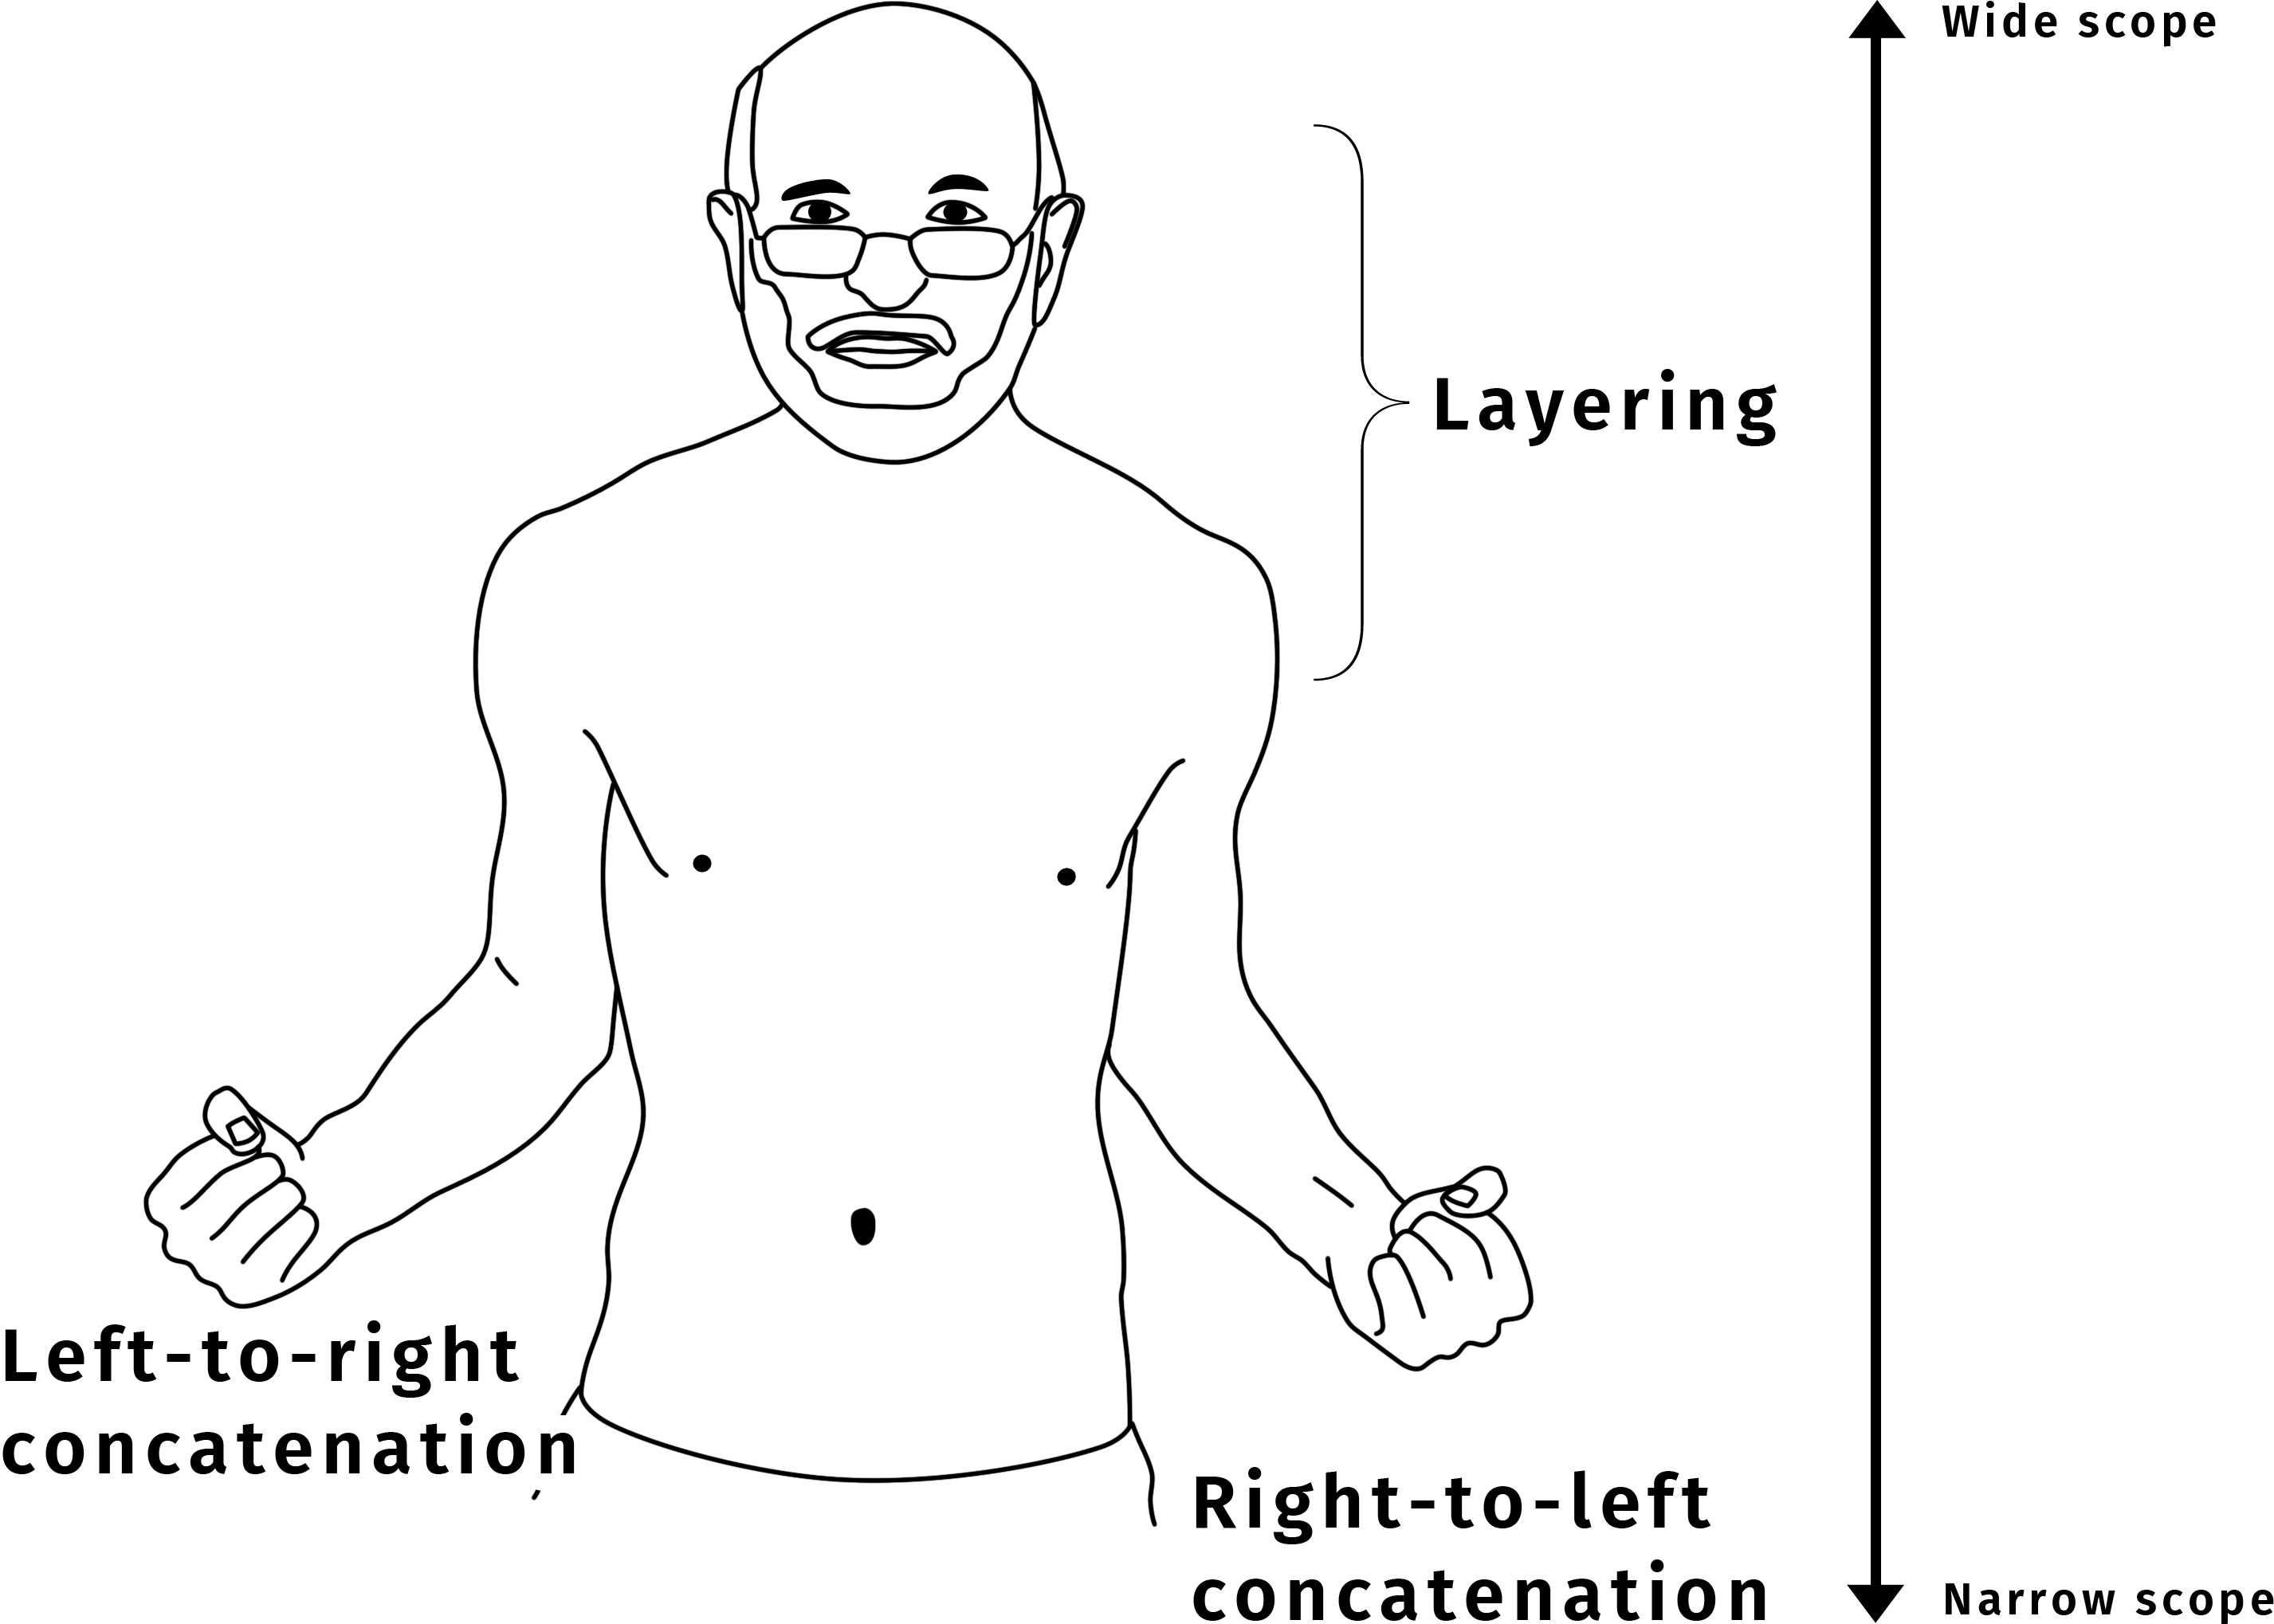
\includegraphics[width=1.0\textwidth]{hypo.jpg}
	\caption{The main hypotheses by \citet{bross2017scope}: Scope is directly mapped onto the signer's body (called the \is{bodily-mapping hypothesis}bodily-mapping hypothesis). The higher the scope, the liklier a category will be expressed via layering and the higher the scope, the higher the articulator. At some point in the syntactic tree, scopal relations are expressed via concatenation, first from left to right, then switching to right to left. The two concatenation strategies are metaphorically depicted as the left and the right hand---although `left' and `right' refers to the relative sequencing of manual signs in time and not to the left or right hand.}
	\label{hypo}
\end{figure}	

\noindent It has to be noted that the vertical mapping of scope proposed by Bross \& Hole does not concern the place of articulation of a manual sign which can be high or low on the body (e.\,g., the forehead versus the abdominal region), but only concerns the articulators themselves. Another important note relates to the fact that there are articulators in sign languages for which it is unclear how high they actually are. It is, for example, clear that the eyebrows are located above the mouth, that the mouth is above the shoulders and that the shoulders are above the hands. If a signer, however, tilts her/his head back, it is rather unclear if the head should be taken to be higher than, lets say, the mouth:\footnote{ There are, of course, many functions fulfilled by movements of, for example, the whole head. As an anonymous reviewer correctly pointed out, single head movements are often observed with focus and repeated head movements (nods) with affirmative functions: This could lead to the speculation that domain marking (repeated nods) and punctual marking (single nods) can also be used to indicate syntactic height. Another hypothesis worth investigating may be the head movements in general are related to truth values. Typical functions which involve movements of the head are negation (head shake), affirmation (repeated nodding), contrastive focus (see Section \ref{contrastivefocussubection}), or epistemic commitment (see Section \ref{polarinterrogativesdgs}).}\label{nesting}

\begin{quote}
A problem to be solved is the question of mereological nesting: Is a body part as a whole, when it performs an action, higher than a subpart of this body part? Is a nodding head, for instance, higher than raised eyebrows or lower? It may turn out that such issues can be resolved empirically by investigating what kind of visual information signers rely on when observing the respective movements. For example, it may turn out that the critical point to evaluate how a nod is perceived is the position of the tip of the nose. If this was the case, then one could convincingly argue that a nod is lower than the eyebrows. \citep[24]{bross2017scope}
\end{quote}

\noindent In the remainder of the book I will mainly concentrate on articulators for which it can be clearly stated that one is above another and exclude claims about the head---at least when it comes to scope-taking. The main hypotheses are depicted in Figure \ref{hypo} (Figure adapted from \citealt[25]{bross2017scope}).

The figure shows that it is assumed that categories taking high scope (i.\,e., CP categories) are expressed via layering. At the same time, descending the hierarchical ordering of clausal categories means descending the body (the bodily-mapping hypothesis). The highest-scoping categories are expressed with the eyebrows and eyes, lower categories with the cheeks and the mouth and even lower categories with the shoulders. Finally, at some point, the strategy switches from layering to concatenation---in German Sign Language, first left to right, then right to left (with left to right for higher and right to left for lower categories). Note that this does not mean that signers use their right or left hands. This is only a metaphorical depiction of sequential ordering of manual signs in time (i.\,e., either O $>$ P or P $>$ O), cf. (\ref{beispielvierzehn}) above. Additionally, note that the claim that the switching from non-manual to manual articulators starts with a left-to-right strategy and then changes to right-to-left is a claim for DGS, while the bodily mapping hypothesis is a claim concerning all sign languages. 

That scope is mapped onto the body in a way that could even be called iconic is, by far, not a necessity (cf. the excursus on iconicity). Quite the contrary: it would be rather plausible to assume that a language in the visual modality would express concrete concepts and not abstract syntactic relations in a truly iconic way. Take the concept of smiling. A sentence like \textit{Marla smiled} could easily be depicted by signing the name sign for Marla and finally performing a smile, as shown in (\ref{ex:smilingexamplea}). However, this is not what we find---neither in DGS nor in any other sign language I am aware of. Instead, the sign for smiling is a manual sign, as shown in (\ref{ex:smilingexampleb}).

\begin{exe}
\ex\label{smilingexample}\begin{xlist} 
\ex \slg{*marla} \slg[smile]{\textcolor{white}{smile}}
%\ex {} {\hspace{41pt}smile}   \\
%{*\textsc{paul}} {$\overline{\textrm{\textsc{\textcolor{white}{smile}}}}$} 
\glt \textcolor{white}{*}`Marla smiled.' \label{ex:smilingexamplea}
\ex \textcolor{white}{*}\textsc{marla smile}  
\glt \textcolor{white}{*}`Marla smiled.' \label{ex:smilingexampleb}
\end{xlist}
\end{exe} 
%

\chapter{Sign languages}\label{chapterone}
In this chapter, I will make some brief remarks on sign languages in general (Section \ref{signlanguagesintro}), about the role of non-manual markings (Section \ref{sectionnmms}), and present some basic facts about DGS (Section \ref{basicclausstructuredgs}). 
%\clearpage
%


\section{Sign languages}\label{signlanguagesintro}
In this section, I will briefly illustrate that sign languages are natural languages with complex grammatical structures obeying the same structural building principles as spoken languages. I will do this cursorily by way of exemplification and illustrate that both spoken and signed languages exhibit duality of patterning\is{duality of patterning|see{double articulation}}\is{double articulation} and that recursion is found in both types of languages -- two features which have been  claimed to be universally found in natural languages (\citealt{martinet1949double}; \citealt{hockett1960origin}). It is nevertheless crucial to note that sign languages are similar to spoken languages in nearly every respect. For example, they serve the same communicative functions, can express meanings in the same way and at the same speed as spoken languages \citep{bellugi1972comparison}, they are naturally acquired by children given normal exposure to the language (e.g., \citealt{newport1985acquisition}), and are processed in the same brain regions as spoken languages (e.g., \citealt{emmorey2002language}). To date, 142 different sign languages with distinct lexicons and distinct grammars with an approximate number of 5\,000\,000 speakers have been documented \citep{simons2018ethnologue}, although it can be assumed that there are more -- perhaps between 300 and 400 different sign languages used all over the world \citep{zeshan2009sign}. That there are so many different sign languages in the world has to do with the fact that sign languages naturally evolve when a sufficient number of deaf people come together over a longer period of time (e.g., \citealt{kegletal1999creation}).

\subsection{The phonology of spoken and signed languages -- duality of patterning}
\is{double articulation|(}
%Thus, sign languages are fully-fledged natural languages. 
While spoken languages are produced by manipulating the air stream flowing through the oral and nasal cavities with the speech organs (the lips, the teeth, the glottis, the tongue etc.), sign languages are produced by the hands, arms, the torso, the head, and the face. Both language types are thus produced by performing gestures with the body. In the case of spoken languages, sound waves hit the eardrums which are set into oscillation. In the case of sign languages, it is light waves which are transformed into electrical signals through receptors within the retina. Differences between sign and spoken languages like these are often referred to as differences in modalities. While spoken languages use the auditory-vocal modality, sign languages make use of the visual-gestural modality. 

While the two language types look very dissimilar on the surface, the structural principles underlying both are astonishingly similar \citep{sandler1989phonology,brentari1998prosodic}. In both modalities, a limited number of elements is used together with a limited number of rules to create an unlimited number of utterances. On the phonological level, for example, spoken languages combine a limited set of phon\-emes (or distinct features creating phonemes), which are by themselves meaningless, to create morphemes carrying meanings (of course, this process is not unconstrained, but governed by phonotactic rules). This way of creating meaning is characteristic of human languages and called `duality of patterning' or `double articulation' \citep{martinet1949double, hockett1960origin}.

In both language types, it is possible to create two morphemes that differ in only one feature, i.e., to create minimal pairs showing that the two features indeed belong to the set of relevant building blocks of the language. In English, the monomorphemic words \textit{cool} and \textit{tool}, for example, only differ in place of articulation of its initial plosive. From this, we can not only infer that the plosives /k/ and /p/ are phonemes of English, but also that the velum (the soft palate) and the alveoli (the tooth sockets) are places of articulation in English used as distinctive features. The same process of minimal-pair formation can be used to determine other parameters which can be used as primary building blocks of a spoken language. One can think of the shape of the lips in vowels, just to give one final example. With vowels, the lips are either rounded, as in /y/, or unrounded as in /i/. In German, this opposition can be used to build minimal pairs. While /ly\textlengthmark g\textschwa / means `lie', /li\textlengthmark g\textschwa / means `cot' or `lounger'. Again, the minimal pairs give us two phonemes, /y\textlengthmark/ and /i\textlengthmark /, and tell us which parameter, in this case rounded versus unrounded lips, is used as a distinctive feature. 

\begin{figure}[bt]
\centering
	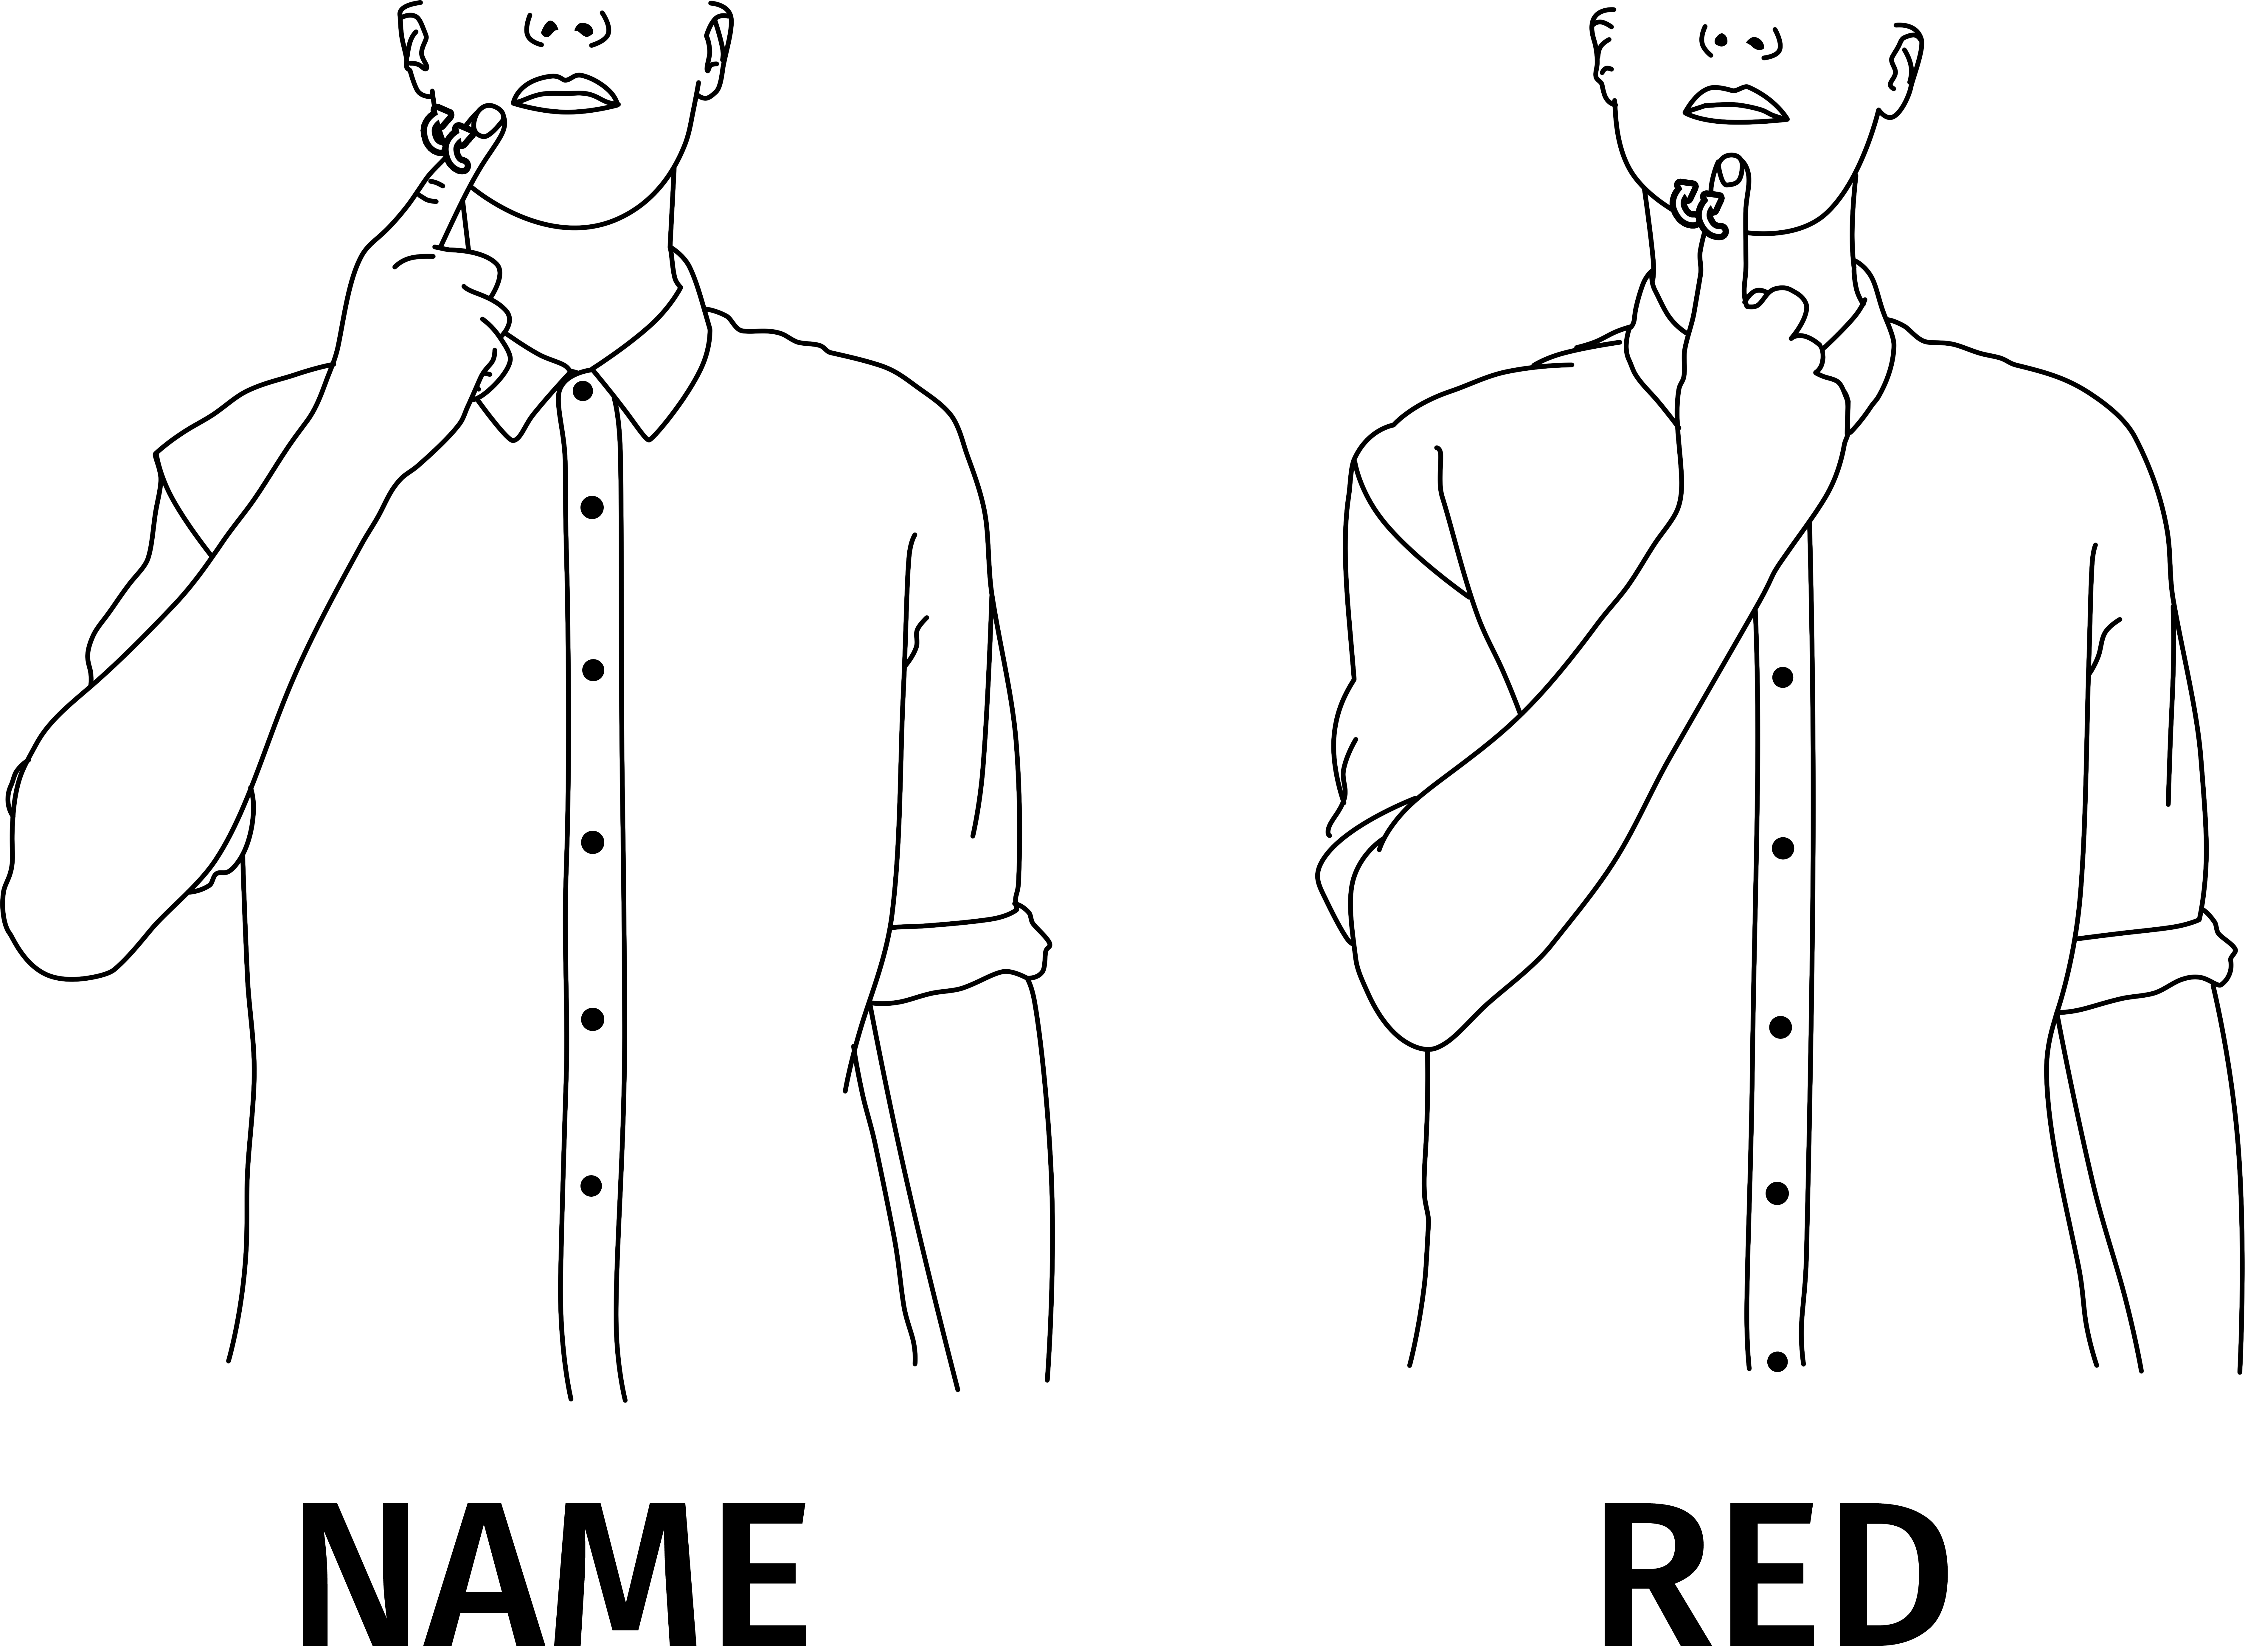
\includegraphics[width=1.0\textwidth]{minimalpair2}
	\caption{An example of a minimal pair resulting from a change in place of articulation. With one variant of the sign \textsc{name} the signer taps her/his cheek two times with her/his index finger, with the sign \textsc{red} this tapping is executed at the chin.}
	\label{minimalpairtwo}
\end{figure}

The exact same processes underlie morpheme formation in sign languages and this, again, can be shown by creating minimal pairs. Sign languages use a limited number of hand shapes, movement directions, places of articulation (often called `locations'), and palm orientations which all have no meaning by themselves\footnote{ It is sometimes claimed that hand shapes, locations, and movements have meaning by themselves (e.g., \citealt[943]{sandler2009sign}). The basis of such claims is the following: an extended index finger, for example, is used as a classifier for human beings in \is{American Sign Language}American Sign Language. This, however, does, in my opinion, not mean that this hand shape has a meaning on its own. The same hand shape is found in signs which have nothing to do with human beings, for example, in the sign \textsc{wheelchair}. Claiming that a hand shape, a location, or a movement has a meaning on its own would be similar to claiming that the phoneme /z/ in English has a meaning on its own, just because it can be used as a plural marker in some words (e.g., \textit{dog} → \textit{dogs}). This, of course, does not exclude the possibility of iconicity at a sublexical level (cf. \citealt{kooij2002phonological,zwitserlood2008morphologybelow}). Thus, it is possible for a sublexical unit to have meaning, but this does not mean that each formational unit has a meaning in every case.} to create morphemes, i.e., larger meaningful units \citep{stokoe1960sign, battison1978}. I will give two examples to illustrate that minimal-pair formation leads to similar results as in spoken languages.\is{distinctive features} Comparable to the English minimal pair \textit{cool} and \textit{tool}, the signs \textsc{name} and \textsc{red} only differ in place of articulation in DGS, as shown in Figure \ref{minimalpairtwo}.\footnote{ The variant of the sign \textsc{name} used here also exists in a variant in which the index and the middle finger is used instead of the index finger only.} Both signs are produced by a reduplicated tapping movement of the index finger. The only difference between the two signs is the place of articulation. While \textsc{name} is articulated on the cheek, \textsc{red} is articulated on the chin. We thus can conclude that the cheek and the chin are places of articulation used in German Sign Language serving as distinctive features. 

\begin{figure}[bt]
\centering
	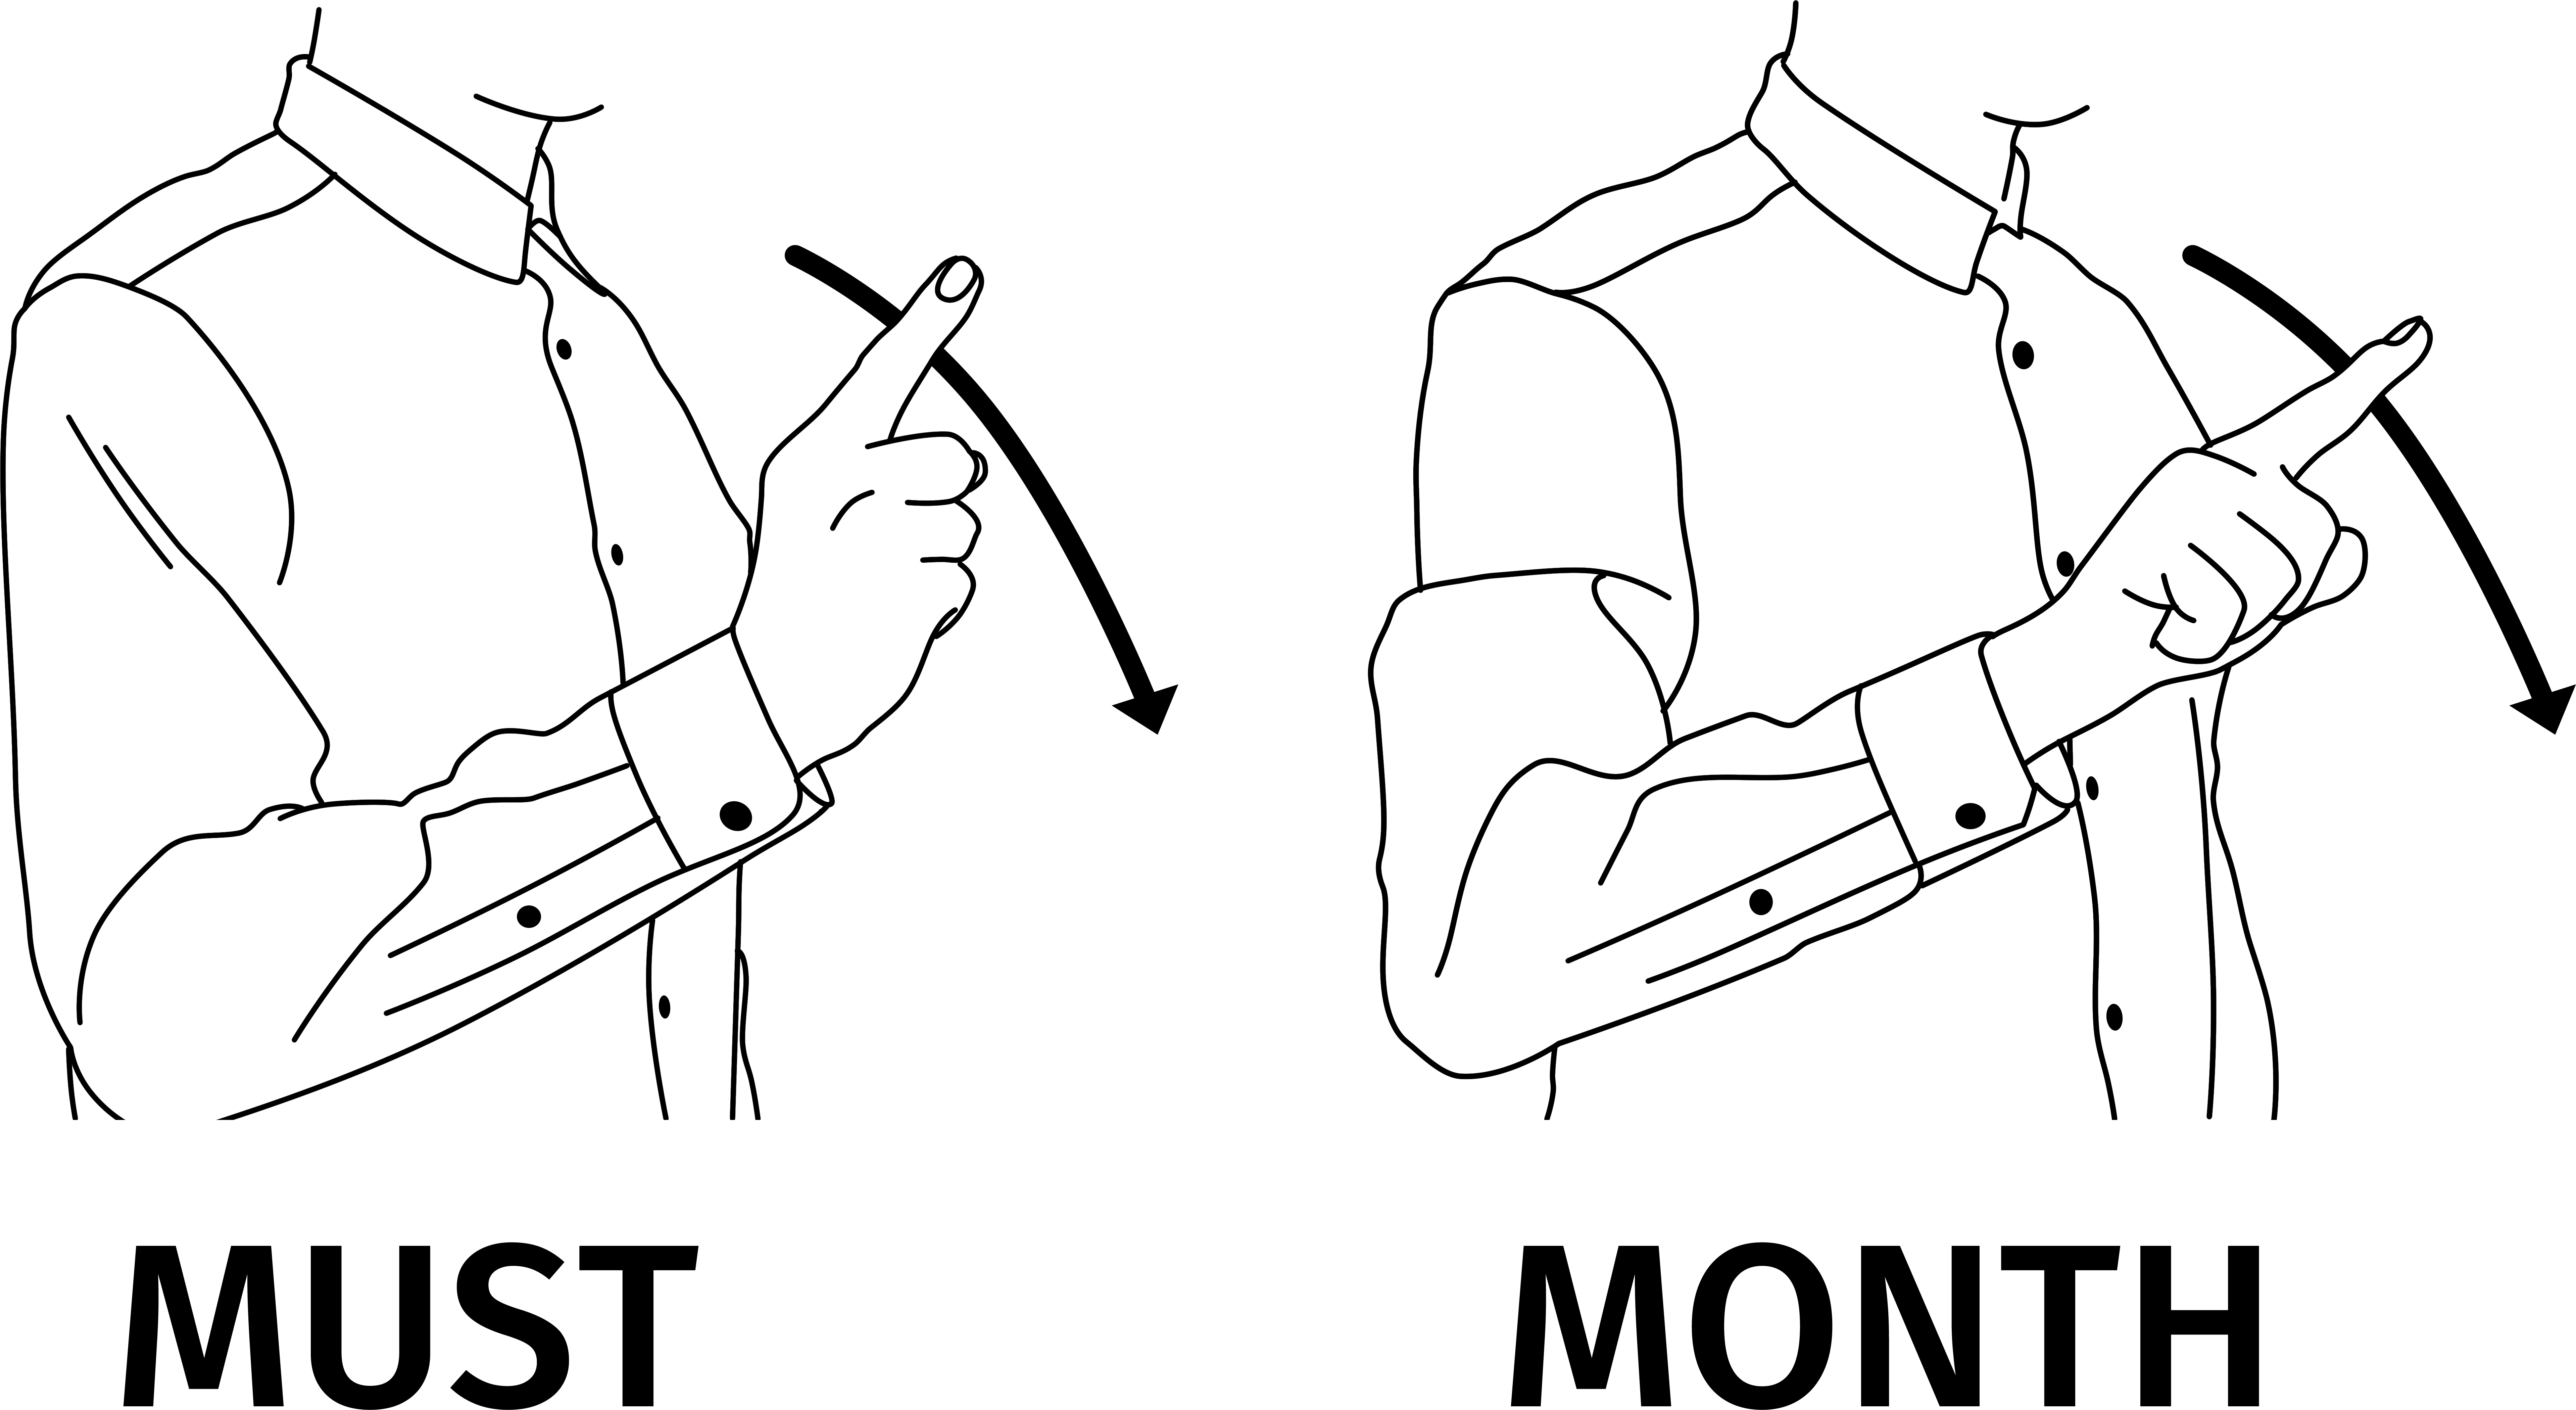
\includegraphics[width=1.0\textwidth]{minimalpair1}
	\caption{An example of a minimal pair resulting from a change in hand orientation. With the sign \textsc{must} the palm faces sidewards, with the sign \textsc{month} the palm faces downwards.}
	\label{minimalpairone}
\end{figure}

Similar to the shape of the lips, the orientation of the palm is used to create meaning differences. In DGS, for example, the signs \textsc{must} and \textsc{month} only differ in palm orientation. Both signs are articulated by a downward movement of the forearm with the index finger extended.  While \textsc{must} is signed with the palm facing sideways, \textsc{month} is signed with the palm facing downwards, as illustrated in Figure \ref{minimalpairone}. From this, we can conclude that the two palm orientations (sideways and face-down) are used as distinctive features\is{distinctive features} in DGS.

Taken together, besides surface differences, spoken and sign languages use the same mechanism to build meaningful elements by using meaningless distinctive building blocks. 


\is{double articulation|)}

\subsection{Building syntactic structures -- embedding and recursion}
Signed and spoken languages are not only similar with respect to double articulation, but on all levels of linguistic description. To give another example, let us take a brief look at embedding and recursion in the syntactic domain. One main feature that has been argued to be fundamental for human languages is that it is possible to take a structure which was produced by applying a syntactic rule and apply the same rule to the structure again (i.e., take the output of a rule and use it as the input for the same rule again). In English, for example, we can build a relative clause introduced by \textit{that} (e.g., \textit{The beer that I bought in the store was delicious}). The product of the applications of this rule (i.e., the relative clause) can now be taken as input for the exact same rule; that is, we can embed another relative clause in the structure (e.g., \textit{The beer that I bought in the store, that is now closed, was delicious}). We can thus create a theoretically infinite sentence applying the same rule over and over again. Structure embedding and recursion are major structure-building processes used in natural languages.\footnote{ There are, of course, other possibilities of building recursive structures besides relative clauses in a language, e.g., affix stacking of the sort \textit{anti-anti-establishment}, adjective stacking, or all kinds of clausal embeddings.} 

Interestingly, early research on American Sign Language\is{American Sign Language} seemed to indicate that similar structures are not possible. In fact, it was claimed that the whole mechanism of subordination was absent in the language as no overt complementizers could be found \citep{thompson1977lack}. However, subsequent research revealed that there are not only relative clauses in sign languages, but that subordination in general is equally possible in this type of language, but only if one knows where to look, as subordination is not marked by manual signs but with non-manual markers in the face \citep{liddell1980american, padden1983action} (for an overview of subordination in sign languages, see, for example, \citealt{gijn2004quest,branchini2014,pfausteinher2016matterofcompl,pfausteinbach2016complexsentences}). In fact, it is not only possible to create relative clauses in sign languages, but they show exactly the same typological variation as spoken languages as both types of languages either used internally-headed relative clauses (e.g., American Sign Language; cf. \citealt{liddell1980american} or \is{Italian Sign Language}Italian Sign Language; cf. \citealt{branchini2014}) or externally-headed relative clauses (e.g., DGS, cf.  \citealt{pfau2005relative}).\footnote{ The picture in fact is far more complex as sign languages exhibiting internally-headed relative clauses usually also have externally-headed relative clauses (see \citealt{wilbur2017internally} for an overview) -- however, not much is known about relative clauses in different sign languages.} And it is, of course, possible, to embed an already embedded structure just like in spoken languages. Although I am not aware of any examples showing that a relative clause can embed another relative clause, it is at least possible to embed a relative clause under another clause as illustrated for American Sign Language in (\ref{ex:relclauseasl}). 

\begin{exe}
\ex American Sign Language \citep[10]{wilbur2017internally}\\ %{\hspace{8pt}top} {} {\hspace{221pt}br} {}  \\
\slg[top]{dog\textsubscript{i}} \slg{index\textsubscript{1} see} \slg[br]{that john say mary chase} $t$\textsubscript{i} \slg{that}
% {$\overline{\textrm{\textsc{dog}\textsubscript{i}}}$} {\textsc{index}\textsubscript{1} \textsc{see}}  {$\overline{\textrm{\textsc{that john say mary chase } \textit{t}\textsubscript{i}}}$} {\textsc{that}}
\glt `I saw the dog that John said that Mary chased.' \label{ex:relclauseasl} 
\end{exe} 

\noindent It is of course nevertheless possible to embed a structure in a structure of the same kind in sign languages. Such a case of real recursion is shown in the DGS example in (\ref{ex:recursion}).\footnote{ The glosses `right' and `left' indicate that the signer turns his/her body and signs the respective signs on the sides of his/her body.}

\begin{exe}
\ex \slg[left]{laura think} \slg[right]{fabian think} \slg{otto sick}
%{\hspace{47pt}left} {\hspace{49pt}right} {}  \\
 %{$\overline{\textrm{\textsc{laura think}}}$} {$\overline{\textrm{\textsc{fabian think}}}$} {\textsc{otto sick}}
\glt `Laura thinks that Fabian thinks that Otto is sick.' \label{ex:recursion}
\end{exe} 

\noindent Taken together, sign languages are natural languages with the same general architecture on all levels of linguistic description, as exemplarily shown for the phonological building processes and embedded structures. In the next section, I will discuss the role of non-manual markings and then present some basic facts about and properties of German Sign Language. Finally, I will discuss the data sources used for the present study.

\section{The role of non-manual markings}\label{sectionnmms}
\is{non-manual markings|(}
Since the very beginnings of sign language linguistics, namely since the seminal work on American Sign Language\is{American Sign Language} by William Stokoe, it has been assumed that non-manual markings, produced simultaneously with the manually signed lexical items, are the ``key to syntactical structure'' \citep[63]{stokoe1960sign}. Research since then has indeed shown that non-manuals, such as eye-gaze, movements of the eyebrows, the head, the upper body, or the shoulders, are cross-linguistically used for syntactic purposes. Examples of constructions which are encoded non-manually in sign languages include topicalizations (e.g., \citealt{aarons1994aspects, aarons1996topics,brunelli2011antisymmetry}), interrogative constructions (e.g., \citealt{neidle2000syntax}; \citealt{zeshan2004interrogative}; \citealt{zeshan2006negative}; \citealt{brunelli2011antisymmetry}), negation (e.g., \citealt{pfau2002applying, roland2002v, zeshan2004negation, zeshan2006negative}), subordination (e.g., \citealt{wilbur1999syntactic, pfau2005relative, cecchetto2006strategies, branchini2009relatively}, tense \citep{zucchi2009along}, or epistemic modality \citep{bross2017scope}. For an overview of the use of non-manuals see also \citet{pfauquer2010nonmanuals}.

Non-manual markings often -- but not necessarily -- are grammaticalized gestures which can also be observed as speech-accompanying gestures in spoken languages (e.g., \citealt{wilcox2004gesture, pfau2006modality, pfau2011grammaticalization}). That such non-man\-u\-al markings, such as eyebrow raise or head shakes, are not gestures anymore, but parts of the grammar of a sign language, can be shown in different ways. The most obvious difference between a gesture and a non-manual marker is its scope and timing. Non-manuals align to well-defined constituents of signed clauses and exhibit clear on- and offsets while the scope and timing of gestures is much more free (e.g., \citealt{bakershenk1983, emmorey1999signers, wilbur2003modality}). Additionally, it has been shown that while facial gestures are processed in the right hemisphere, grammatical non-manual markers of the face are processed in the left hemisphere, as would be expected for linguistic signals \citep{corina1989recognition}. Consequentially, right hemispheric brain lesions can lead to impairments of affective, but not grammatical, facial expressions \citep{kegl1991interplay, poizner1992neural, loew1997fractionation, corina1999neuropsychological}. The other way around is also true: lesions in the left hemisphere lead to an impairment of grammatical, but not affective, facial expressions \citep{kegl1997crosslinguistic}.

It is often assumed that non-manual markers in sign languages are equivalent to intonation in spoken languages (e.g., \citealt{sandler1999prosody}). This is plausible as both are suprasegmental structures. Additionally, both are used for similar functions. For example, all sign languages studied so far use non-manual markers, usually an eyebrow raise, to indicate polar interrogatives. Similarly, intonation is often used to mark polar interrogatives in spoken languages. However, not all non-manuals are similar to intonation in this respect. A head shake, frequently used in sign languages to mark negation, for example, can hardly be equated with intonation as suprasegmental means are rarely used in spoken languages to mark negation.

While the comparison of non-manual markings to intonation is a purely phonological claim, on the syntactic side it has been argued that non-manuals are ``frequently associated with syntactic features residing in the heads of functional projections'' \citep[43]{neidle2000syntax}. Additionally, it was often assumed that the spread of the non-manuals marks their c-command domain and that the greatest intensity of the non-manual markers is at its position of origin (\citealt{bahan1996}; \citealt{petronio1997}; \citealt[43--45]{neidle2000syntax}; \citealt[311--312]{sandler2006sign}).\footnote{ Note that this is not the case with topicalizations as non-manuals only mark the topic, but not the whole clause in the c-command domain.} Concerning the hypothesis that non-manuals are associated with head features, I will defend the view that non-manuals are not (necessarily) syntactic heads, but rather reflexes of Spec-head agreement. I will call this the `Non-Manuals as Syntactic Markers Hypothesis':

\begin{exe}
\ex \textit{Non-Manuals as Syntactic Markers Hypothesis:}\\
Non-manuals do not spread uniformly across constituents, but have an intensity peak at some point. This point, the intensity peak of the non-manuals, marks the location of a syntactic head triggering the non-manuals via Spec-Head agreement. Additionally, the spread of the non-manuals may mark the c-command domain of this head. \label{nmasmh}
\end{exe}

\noindent If \citeauthor{neidle2000syntax}'s (\citeyear{neidle2000syntax}) claim that non-manuals spread over the c-command domain of the head triggering them is correct, it is interesting to note that different non-manual markers are generally assumed to have different spreading domains regarding their location on the signer's body. For non-manuals produced with the face, for example, it has often been noted that a general split exists between non-manuals produced with the upper and those produced with the lower face. While upper-face non-manuals seem to be associated (cross-linguistically) with larger domains and usually fulfill syntactic functions, lower-face non-manuals have a smaller spreading domain and are usually associated with one phrase (e.g., \citealt{liddell1980american, coerts1992nonmanual, wilbur2000phonological, wilbur2003modality, brentari2002prosody}). \citet[249]{wilbur2009productive}, for example, notes: 


\begin{quote}
The lower part\label{wilburquote} of the face tends to produce meaningful markers (adjectives, adverbs) that associate with specific lexical items or phrases with those lexical items as heads (e.g., N or NP, V or VP). The upper part of the face (eyebrows, head position, head nods, eyegaze) tends to co-occur with higher syntactic constituents (clauses, sentences) even if such constituents contain only a single sign (e.g., a topicalized noun). 
\end{quote}

\noindent This general split between the upper and lower face is illustrated in Figure \ref{upperlowerfacedivisionoflabour}. See also the main hypothesis underlying the present study discussed in Section \ref{hypotheses}.

\begin{figure}
\centering
	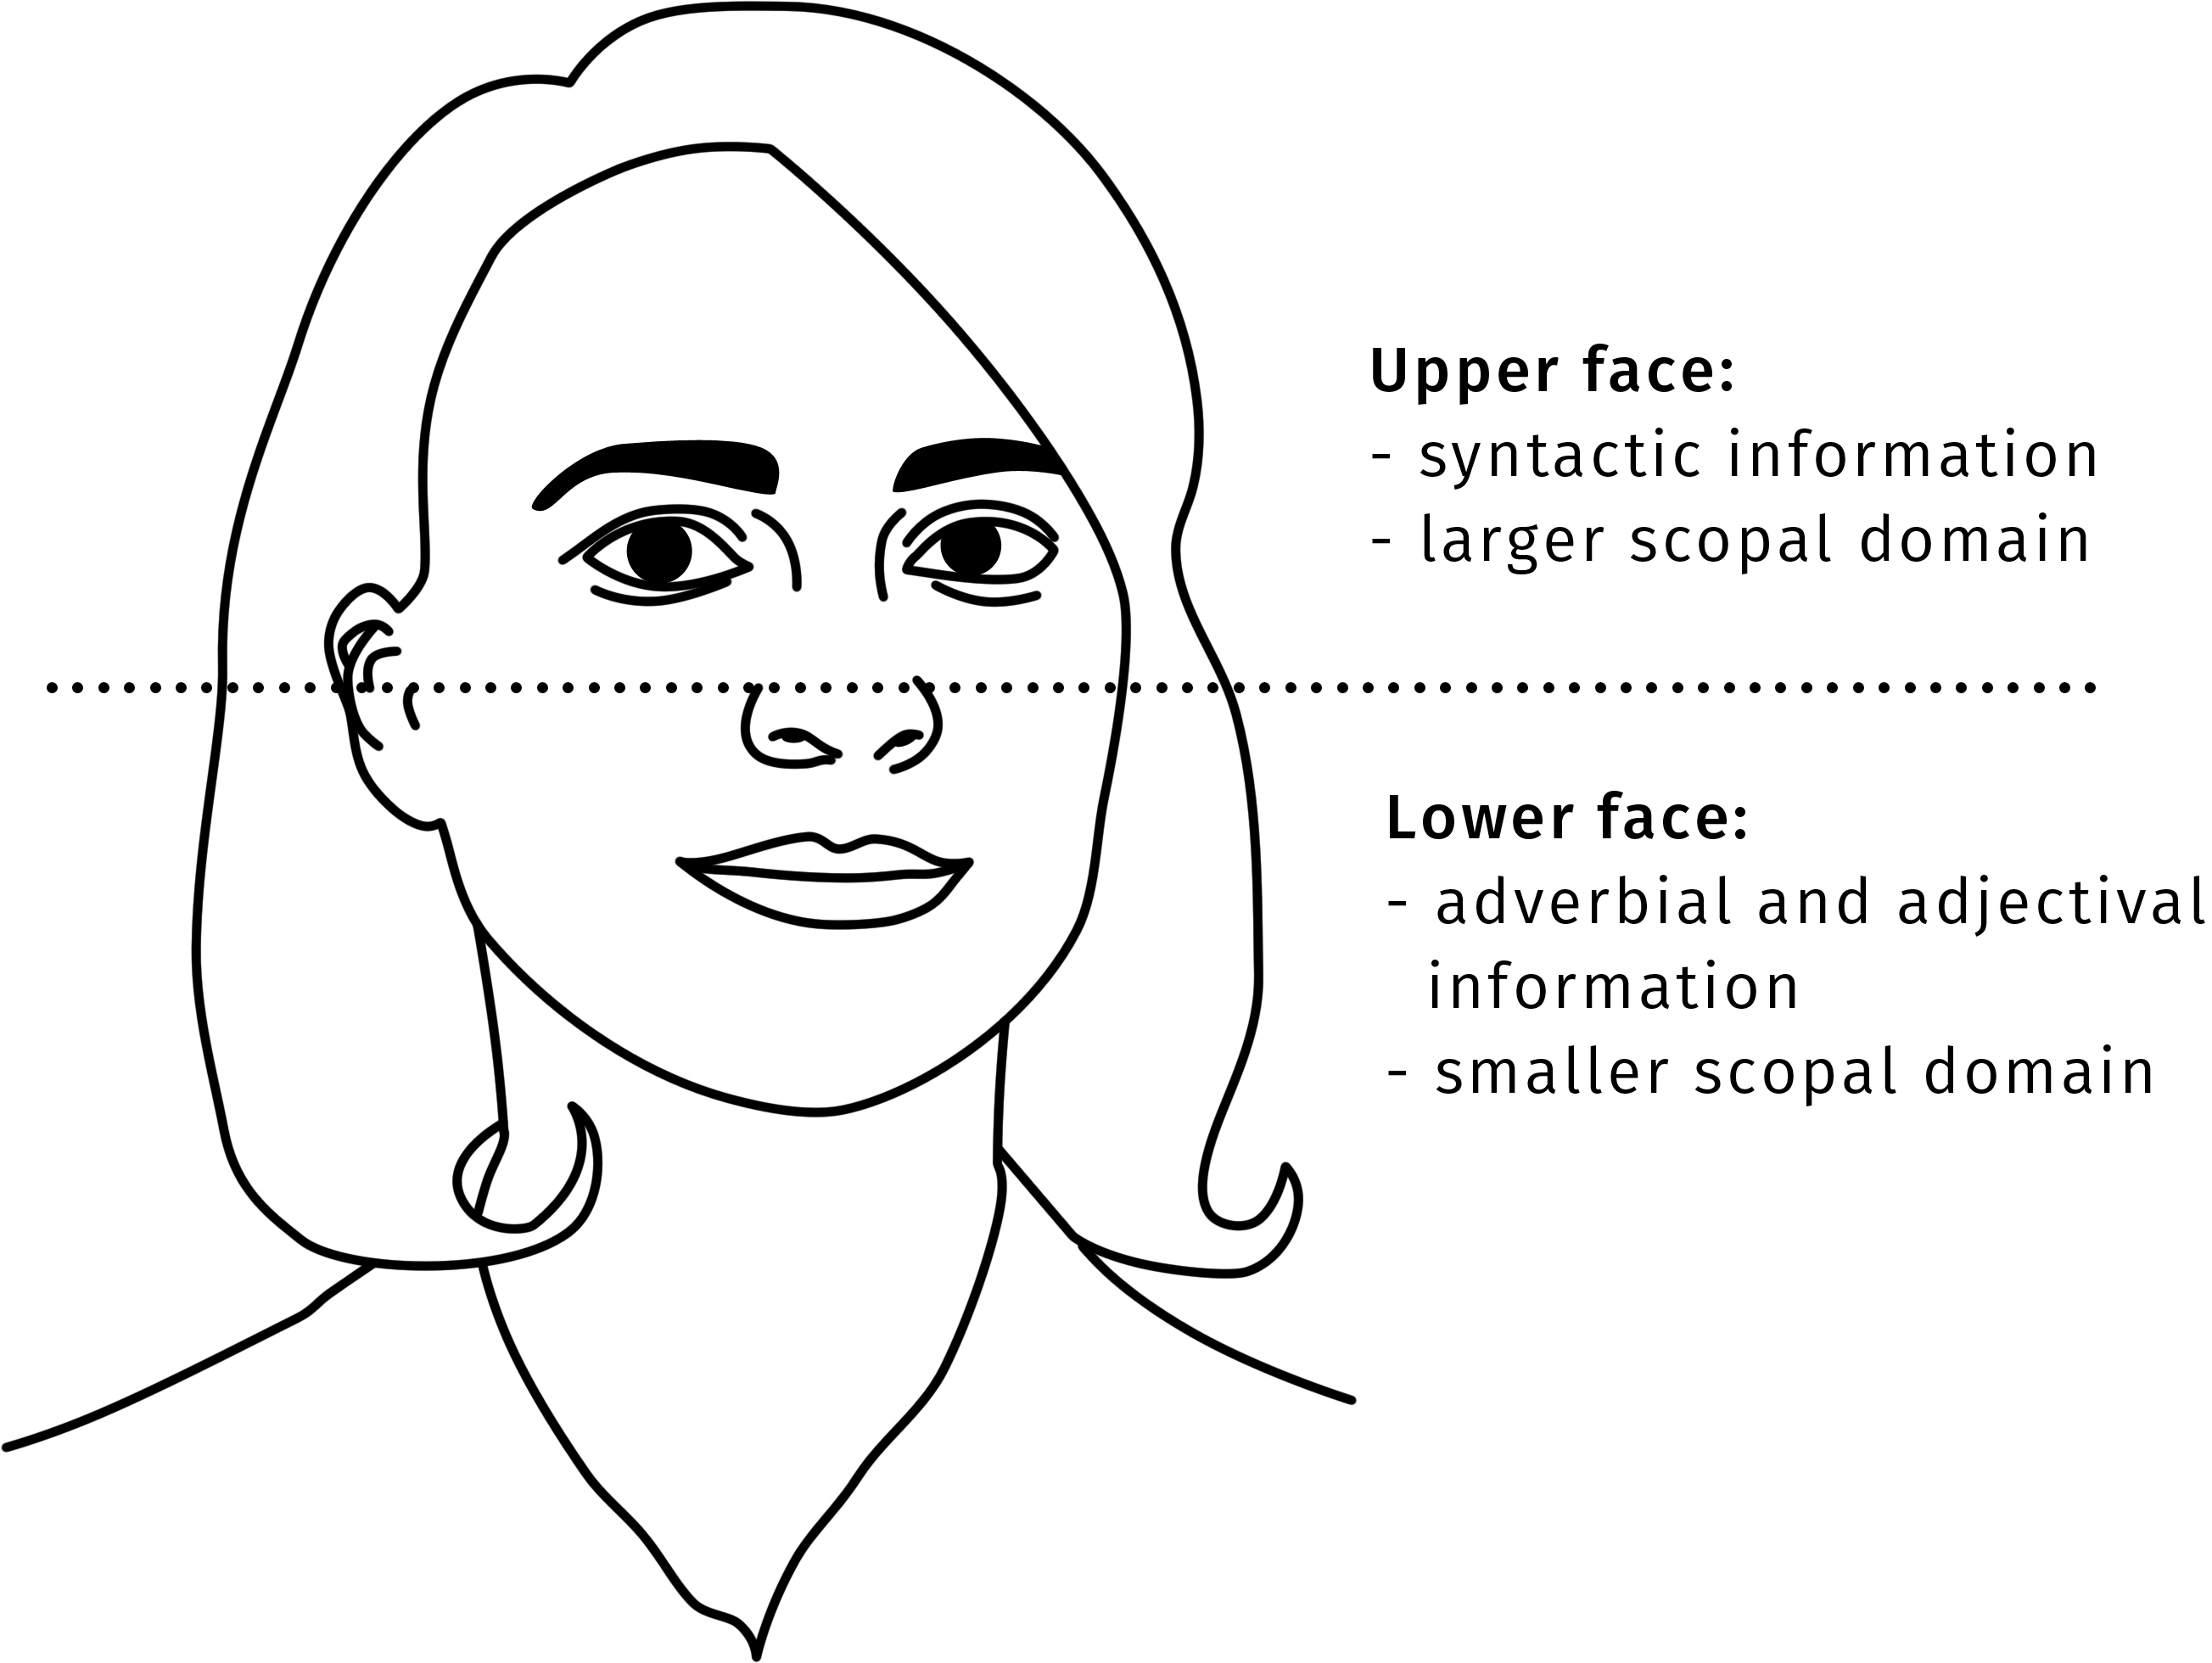
\includegraphics[width=.6\textwidth]{face}
	\caption{The division of labor of the upper and lower face found in many sign languages.}
	\label{upperlowerfacedivisionoflabour}
\end{figure}


It has to be noted that non-manual markers usually come in bundles. It would be desirable to identify one marker for a specific function, for example, eyebrow raise for marking a polar interrogative. However, it turns out that this is often a difficult task, although it has been repeatedly proposed that non-manual markers combine compositionally (e.g., \citealt{nespor1999prosody, sandler2006sign, dachkovsky2009visual, herrmann2013modal}). I will describe this problem in more detail for questions which are not only marked by eyebrow movements in DGS, but additionally by putting the head forward and tilting it sideways in sections \ref{polarinterrogativesdgs}, \ref{whinterrogativedgs}, \ref{rhetq}, and \ref{perhapsmoodirrealis}. There, I will show that such a compositional analysis is indeed possible. I will argue that the eyebrows are used to clause-type a sentence; that the head is put forward to indicate that an answer or other reaction is expected; and that sideways head tilts are used to express the degree of epistemic commitment.\is{non-manual markings|)}

\section{German Sign Language}\label{basicclausstructuredgs}


German Sign Language (\textit{Deutsche Gebärdensprache}, DGS) is a sign language used mainly in Germany. The number of DGS users can only be estimated. A frequently cited number is 80\,000. This number, however, is only an estimation of the amount of deaf people in Germany (e.g., \citealt{dgb}) which is often equated with the number of deaf sign language users in Germany (e.g., \citealt{herrmann2007,schwagerzeshan2010}). However, it is in fact not exactly clear how many deaf individuals there are in Germany. The Federal Office of Statistics, for example, estimates that there are around 28\,000 deaf people without cognitive impairments living in Germany \citep{schwerbehindertenstatistik2017}, a number that is much smaller than the usually cited 80\,000. Of course, not all deaf people might use sign language and there are also hearing people using DGS. Finally, many hard of hearing individuals also use DGS and the number of hard of hearing individuals is much higher than the number of deaf people. The Federal Office of Statistics assumes that there are over 250\,000 hard of hearing people living in Germany \citep{schwerbehindertenstatistik2017}. Thus, on some estimates, the number of DGS users is much higher. The European Union of the Deaf \citep{eud2012} or the Ethnologue \citep{simons2018ethnologue}, for example, assume that there are approximately 200\,000 users of DGS in Germany.

DGS is a rather strict SOV language in both matrix and subordinate clauses (e.g., \citealt{keller1998aspekte, pfau2001pseudo}). As would be expected from a SOV language, modal verbs generally appear in a clause-final position, as shown in (\ref{modalverbplacement}) (although there is some variation to the placement of modal verbs, as discussed in \chapref{ipsystem}). 


\begin{exe}
\ex \textsc{elias perform-magic can}
\glt `Elias can perform magic.'\label{modalverbplacement}
\end{exe}

\noindent As DGS is an OV language and as modal verbs occur clause-finally, it is usually assumed that heads of functional projections are to the right (e.g.,  \citealt[365]{sandler2006sign}; \citealt[17]{herrmann2013modal}; \citealt[3]{bross2017scope}). This leads to a basic clause structure as represented in (\ref{ex:basciclausstructure}). Note that one of the most controversial topics related to the clause structure of DGS is the question of whether SpecCP is to be located on the left or on the right. I have put SpecCP provisionally on the left in the tree as this is a widely-held opinion (e.g., \citealt{herrmann2013modal}) and will discuss the exact position in detail in the next chapter (in detail in Section \ref{whinterrogativedgs}).

%\begin{exe}
%\ex \label{ex:basciclausstructure}
%\begin{tikzpicture}[baseline=(current bounding box.north), scale=0.8]
%\tikzset{level distance=35pt,sibling distance=5pt,every tree node/.style={align=center,anchor=north}}
%%\tikzset{sibling distance=1pt}
%\tikzset{every tree node/.style={align=left,anchor=north}}
%\Tree [.CP [.{SpecCP} ] [.{$\overline{\textrm{C}}$} [.IP [.{SpecIP} ] [.{$\overline{\textrm{I}}$} [.VP [.{SpecVP} ] [.{$\overline{\textrm{V}}$} [.{} ] [.{V\textdegree } ] ] ] [.{I\textdegree } ] ] ] [.{C\textdegree } ] ] ]
%\end{tikzpicture}
%\end{exe}

\begin{exe}
\ex \label{ex:basciclausstructure}
\begin{forest}
for tree={s sep=25mm, inner sep=0, l=12mm} %s sep = Breite; l = Höhe
[CP [SpecCP] [$\overline{\textrm{C}}$ [IP[SpecIP][$\overline{\textrm{I}}$[VP[SpecVP][$\overline{\textrm{V}}$[{\phantom{V}}][V\textdegree]]][I\textdegree]]][C\textdegree]]]
%[CP[C][IP[I][VP[V][NP]]]]
\end{forest}
\end{exe}


\clearpage

\noindent In many cases, the SOV order can be altered by fore- and backgrounding processes such as topicalizations. Additionally, word order is affected by the figure-ground principle. I will have more to say about word order in Section \ref{declarativesentences} and discuss topicalizations in Section \ref{topicsindgssection}. 



DGS is a comparatively well-studied sign language. Consequently, there is a vast literature on many aspects of the language. Besides more descriptively oriented grammars \citep{papaspyrou2008grammatik,happ2014vork} and research from a more applied perspective \citep{eichmannhansenhessmann2012,dumig2013}, works on language acquisition (e.g., \citealt{leuninger1997lena,hanel2005spracherwerb,haenelfaul2012erwerb}) or the phonological structure (e.g., \citealt{benner2012,herrmann2012prosody,dumig2013}) from various frameworks, there is a huge Generative research tradition. Within this tradition, various topics have been addressed, including negation \citep{pfau2008headshake,pfau2016featural}, relative clauses \citep{pfau2005relative}, agreement \citep{pfau2006thedevelopment,steinbach2007grammaticalization,steinbach2011agreement,pfausalzmannsteinbach2018agreement}, pluralization \citep{pfausteinbach2004}, role shift \citep{hermannsteinbach2012quotation}, or modality \citep{herrmann2007,herrmann2013modal} -- to name but a few.

Research on DGS has so far mainly concentrated on the variants used in the areas in which the large sign language research centers are located -- most notably, in Göttingen in central Germany, Hamburg in northern Germany where the DGS corpus project \citep{jahn2018} is hosted, Berlin in north-eastern Germany and in a former center in Frankfurt in south-western/central Germany. The data presented in this book, in contrast, comes from southern Germany. The DGS variant used in southern Germany is very similar to the sign language used in the rest of Germany, although there are some dialectal differences in vocabulary and also some syntactic differences which mainly concern negation and contrastive focus (at least as far as I am aware of). These are described in Section \ref{contrastivefocussubection} (see page \pageref{contrastivefocus}) and Section \ref{imperativesindgs} (see page \pageref{negationnegaation}) respectively. 

%\clearpage

\largerpage
\section{Data sources}\label{methods}
The data presented in this book were elicited from nine native signers of German Sign Language living in the states of Bavaria (six individuals) and Baden-Württemberg (three individuals) in southern Germany. Eight of them are deaf and one is a hearing child of deaf adults (CODA). Six of the signers acquired sign language from birth, three are early learners, defined as individuals who started acquiring sign language before the age of four (one acquired DGS since the age of two, one at the age of one and a half, and one since the age of three). Additionally, data from two late-learners were collected. Both late learners are deaf from birth and visited deaf schools, but reported that they did not use German Sign Language, but manually coded German in school. The age range of the signers was between 20 and 56, the mean age was 28.44 (\textit{SD} $=$ 6.04). Four of them were men. It was ensured that all consultants had proficient written language skills and all of them had at least a high-school diploma (a German \textit{Realschulabschluss}). 



The data were elicited in face-to-face interactions which were recorded on video. There was a total of 16 sessions. Each session lasted for about 2 hours. Consultants received the (written) material to be discussed one week before the video recordings to familiarize themselves with the meanings of the sentences. At the actual recording sessions, the sentences (or mini-dialogues) were presented on sheets of paper. In many cases, the sentences were presented with context sentences to arrive at the desired reading. Each sentence was presented to them for a few seconds. The consultant read the sentence and had some time to think about its meaning. Then the sheet of paper was covered up. After the sentence was covered up, the consultants again had some time to think about the meaning of the sentence. 

\largerpage
Then they signed what they thought was the best way to express this meaning in German Sign Language. This procedure was chosen to prevent the  signers  from  being  influenced  too  much  by  the  sentence's  written  structure. All translations were videotaped. In many cases, after the sentence was signed, the sentence and possible paraphrases were discussed. Additionally, the  consultants often were explicitly asked for grammaticality judgments (or rather acceptability ratings). Examples of sentences with contexts (in brackets) are given in (\ref{examplematerial}) (of course, the original sentences were in German). The contexts ensure that the example in (\ref{examplemateriala}) receives a deontic and the sentence in (\ref{examplematerialb}) an epistemic interpretation, respectively.

\begin{exe}
\ex\label{examplematerial}\begin{xlist}
\ex (Paul's parents are strict). Paul must be at home at 8 o'clock. \label{examplemateriala}
\ex (The light in Paul's room is on.) Paul must be at home. \label{examplematerialb}
\end{xlist}
\end{exe}

\noindent In line with previous studies (e.g., \citealt{herrmann2013modal}), it turned out that signers used manual modal verbs (in this case the sign \textsc{must}) in deontic examples like the one in (\ref{examplemateriala}), but did not use manual modal verbs in epistemic examples like the one in (\ref{examplematerialb}). Instead, sentences with epistemic meanings are marked non-manually with a squint (see Section \ref{sectionepistemic} for more details). Signers were then asked if the examples could be signed without the non-manuals or by adding a manual modal verb. Usually, this was done by repeating the example with the aforementioned changes by the author. Examples including deontic modals did not receive non-manual markings spreading over the whole clause, but the manual modal signs themselves were sometimes marked non-manually (in the case of deontic necessity modals: increased signing speed of the modal verb, lowered and squinted brows accompanying the modal). Again, signers were asked if the sentence could be signed without the non-manuals, while still being acceptable and conveying the relevant meaning. In some cases, it then turned out that the non-manuals were not obligatory, as with deontic modality, in other cases, as in sentences with epistemic meanings, the non-manuals cannot be omitted without a change in meaning. 

The signed sentences were cut into separate video files using Adobe Premiere Pro CC. Each file was annotated for the relevant category (e.g., deontic modality). On the whole, this resulted in 1229 video files. The subsequent analysis was not a quantitative, but an incremental qualitative one. The available videos of each category at one point in time were compared, for example, concerning the non-manuals on different levels (upper face, lower face, head movements) to filter out idiosyncrasies of single signers. Remaining questions were used as a point of departure for the next data elicitation sessions. In the case of polar interrogative sentences, for example, it turned out that the consultants raised their eyebrows, put their heads forward and to the side (see Section \ref{polarinterrogativesdgs} for details). While the eyebrow raise was consistently used by all consultants, putting the head forward and putting it to the side was not present in all instances. After consulting the literature on questions, it was hypothesized that each of the non-manuals would fulfill a specific function. Functions hypothesized to be present were, for example, (i) that the signer does not know the truth of the proposition expressed, (ii) that the signer wants to know the truth value of the proposition expressed, or (iii) that the signer believes that the interlocuter being asked knows the truth about the proposition embedded in the question (e.g., \citealt[4]{dayal2016questions}). Subsequently, examples (minimal pairs, if possible) were created in which one function was missing. In the case of polar interrogatives, rhetorical questions were, for example, elicited to scrutinize what happens if the signer does not expect an answer.

One potential problem with this kind of data elicitation is that the signers could be influenced by the grammatical structure of the German sentences. Although such concerns have to be taken seriously, the fact that many of the constructions discussed in this book differ drastically from spoken German can be taken as a strong indication that the influence of spoken German was at least not very substantial (see \citealt[281]{cecchetto2009another} for a similar argument).

Another problem relates to the tension between what \citet[26]{zyman2012two} called the ``breadth approach'' and the ``depth approach''. When investigating a linguistic phenomenon P in a language L, the researcher either collects the same judgments from a large number of native speakers of a language (the breadth approach) or collects different judgments from a smaller number of native speakers (the depth approach). While the breadth approach has the advantage of being more precise, it comes with the cost that P can be investigated in less detail. The depth approach, in contrast, has the disadvantage of being less precise in which aspects of P may be subject to inter-speaker variation, but it has the advantage of enabling the researcher to get a broad picture of P and its subphenomena.

As this book is concerned with a large number of different categories and how they combine it was not possible to collect judgments for each example presented from each consultant. I thus adopted the depth approach to study the clause structure of DGS in more detail. Nevertheless, care was, of course, taken that each judgment was confirmed by several signers. However, it has to be stressed, as \citet{zyman2012two} also notes, that both approaches need to be pursued as they complement each other. I am thus convinced that many of the phenomena discussed in this book need to be studied in more detail in the future. 

The same is, of course, true of the spoken language examples presented in this book which are not taken from the literature. I consulted two native speakers of Turkish, two Mandarin native speakers, and three native speakers of the Northern Italian dialect spoken in Sommacampagna (Custoza) to collect acceptability indications for these examples.



\section{Outline of the book}\label{outlinesection}
The present book consists of three main chapters reflecting the three main layers of the clause, the CP, the IP, and the VoiceP layer. Each section in all three chapters basically has the same structure. I will first generally introduce the phenomenon under discussion by briefly sketching what is known about it in spoken languages. Then, I will sketch what the literature has to say about the phenomenon in sign languages and finally discuss my own DGS data. 

In \chapref{cpchapter}, I will discuss the CP system of DGS. After a discussion of topic and focus marking in DGS I will describe how DGS encodes different sentence types. Besides the main sentence types, declaratives, polar and constituent interrogatives, as well as imperatives, the chapter will also be concerned with some minor sentence types, namely alternative questions, degree questions, tag questions, suggestive questions, rhetorical questions, and optatives. In \chapref{ipsystem}, I will go through the categories discussed in \citet{cinque1999adverbs, cinque2006restructuring}. Some of these categories are located above tense and thus could be considered to still belong to the CP system. The majority of categories, however, are located below tense, but above the VoiceP. In \chapref{insidevp}, the remaining Cinquean categories below the VoiceP layer will be discussed. Finally, in \chapref{chapterconclusions}, I will conclude the findings.


\chapter{The CP system}\label{cpchapter}
In this chapter, the structure of the Complementizer Phrase (CP) will be explored. First, a general overview of the structure of the CP will be given in Section \ref{introcpchapter}. Then the following topics will be discussed: In Section \ref{generaltopicsection}  and \ref{generalfocussection}, I will discuss topic and focus. The remainder of the chapter is devoted to the encoding of different sentence types in DGS including declaratives (Section \ref{declarativesentences}), polar interrogatives (Section \ref{polargeneralsectionlabel}), constituent interrogatives (Section \ref{constint}) imperatives (Section \ref{generalsectionimperatives}), and optatives (Section \ref{opt}).

In each section one phenomenon will be discussed and each section has the same general structure: First, I will introduce the phenomenon, its expression and its analysis in spoken languages, then I will give a brief overview of what is known about the phenomenon in sign languages and how it has been analyzed in the sign language literature. Finally, I will discuss and analyze the phenomenon in German Sign Language.

As will become clear throughout the chapter, all high CP functions find their expression non-manually in DGS. In line with the \is{bodily-mapping hypothesis}bodily-mapping hypothesis by \citet{bross2017scope} (cf. Section \ref{hypotheses}), I will show that all sentences types (except declaratives that are left unmarked) are mainly marked with the highest possible articulator, i.\,e., the eyebrows. For the other high CP categories that (traditionally) do not fall under the labels `sentence type' or `speech act', I will show that they also find their expression non-manually with the upper face. This is true for topic and focus marking. In the case of topic marking, two types of topics are distinguished, each receiving different eyebrow markings: base-generated and moved topics. Concerning focus, I will show that while information focus mainly stays unmarked, contrastive focus is marked by a combination of head and eyebrow movements. Taken together, this provides not only strong support for the hypothesis that structurally high categories are expressed non-manually, but also for a stronger version of the \is{bodily-mapping hypothesis}bodily-mapping hypothesis, i.\,.e, for the idea that the higher a structure is located syntactically, the higher the body part will be that is used to express it. In the end, it will become clear that all CP categories are expressed with the upper face (or a combination of the upper face and another articulator).

\section{Introduction: the organization of the CP}\label{introcpchapter}
The goal of this section is to introduce the structure of the CP, the highest clausal structure, also called the `left periphery' of a clause. The CP serves as an interface as it connects a clause to the structurally higher ``outside'' of itself. Depending on the form and function of the clause, this ``outside'' can be rather different. Two main cases can be distinguished: a clause can be an independent main clause or it can depend on another clause and thus be an embedded clause. 

In the case of a main clause, the ``outside'' is the discourse. The CP system then is able to host finiteness, topics, and focus and indicates the mood of the clause. The terms `topic', `focus', and `mood' need more clarification. I will provisionally define the topic of a sentence as the information the sentence is about \citep{reinhart1981pragmatics}, the focus as the new information in a sentence, and sentence mood as encoding whether we are dealing with a declarative, interrogative, imperative etc. sentence. More precise definitions will be given in the sections to follow. If the clause is not a main clause, but rather an embedded clause, the function of the CP is to connect the embedded clause with the structurally higher clause. In this case, it has often been observed that CPs of embedded clauses are structurally impoverished compared to main clauses (e.\,g. \citealt{haegeman2003conditional}, but see \citealt{haegeman2013syntax} for an alternative analysis). Taken together, the CP is thought of as being ``the interface between a propositional content [\dots ] and the superordinate structure (a higher clause, or possibly, the articulation of discourse [\dots ])'' \citep[283]{rizzi1997fine}.

\subsection{The landing site of \textit{wh}-movement}

The CP itself\is{wh-movement@\textit{wh}-movement} was introduced in the mid 1980s as functional categories were integrated into the $\overline{\textrm{X}}$-schema (e.\,g., \citealt{chomsky1986barr, speas1986ecifiers}). At this time, each of the main layers in a clause, the CP, the IP/TP, and the VP, consisted of a single projection, i.\,e., of a combination of a specifier, an intermediate projection $\overline{\textrm{X}}$, a head, and a complement. The specifier of the CP was thought of as being the landing site of \textit{wh}-movement. This can be easily illustrated for English. 

While English indicative main clauses exhibit a basic S-V-O order, or in clauses containing an auxiliary verb, an S-Aux-V-O order, a constituent interrogative clause has the structure wh(O)-Aux-S-V when it is the object that is being asked for. Consider the examples in (\ref{ex:basiccpstructurea}) and (\ref{ex:basiccpstructurba}) respectively for illustration.


\begin{exe}
\ex\begin{xlist} 
\ex Kassandra will eat an apple. \hfill S-Aux-V-O\label{ex:basiccpstructurea}
\ex What will Kassandra eat? \hfill wh(O)-Aux-S-V \label{ex:basiccpstructurba}
\end{xlist}
\end{exe} 

\noindent The example in (\ref{ex:basiccpstructurea}) shows a basic S-Aux-V-O structure. If one wants to know what it is that Kassandra will eat, the corresponding question looks as in (\ref{ex:basiccpstructurba}) where the object of Kassandra's eating is fronted to a position that was thought of as being the specifier of the CP. The tree structures of the two examples are depicted in (\ref{ex:basiccpstructureaa}) and (\ref{ex:basiccpstructureab}) in an approximate mid-to-end-1980s format.

\begin{exe}
\ex
\begin{multicols}{2}
\begin{xlist}
\ex \label{ex:basiccpstructureaa}
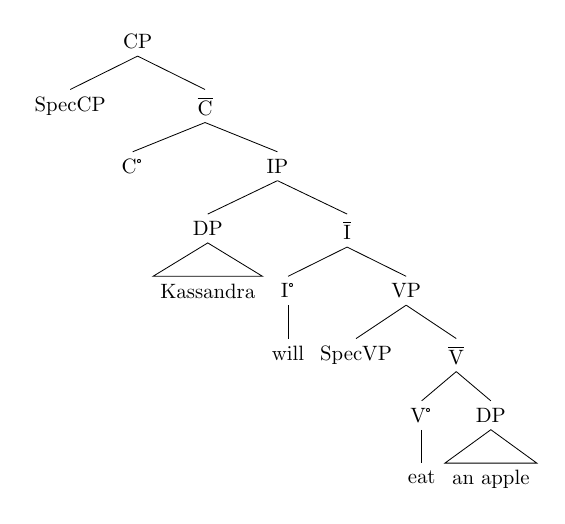
\begin{tikzpicture}[baseline=(current bounding box.north), scale=0.75]
\tikzset{sibling distance=1pt}
\tikzset{every tree node/.style={align=left,anchor=north}}
\Tree [.CP [.SpecCP ] [.{$\overline{\textrm{C}}$} [.{C\textdegree } ] [.IP [.DP \edge[roof]; {Kassandra} ] [.{$\overline{\textrm{I}}$} [.{I\textdegree } will ] [.VP [.SpecVP ] [.{$\overline{\textrm{V}}$} [.{V\textdegree} eat ] [.DP \edge[roof]; {an apple} ] ] ] ] ] ] ]
\end{tikzpicture}
\ex\label{ex:basiccpstructureab}
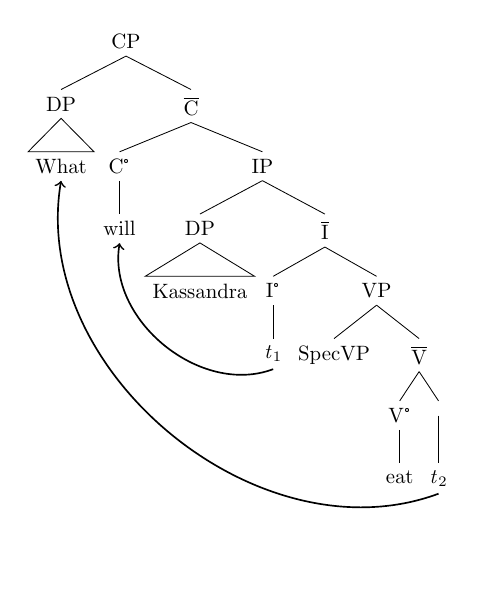
\begin{tikzpicture}[baseline=(current bounding box.north), scale=0.75]
\tikzset{sibling distance=1pt}
\tikzset{every tree node/.style={align=left,anchor=north}}
\Tree [.CP [.DP \edge[roof]; \node(what){What}; ] [.{$\overline{\textrm{C}}$} [.{C\textdegree } \node(will){will}; ] [.IP [.DP \edge[roof]; {Kassandra} ] [.{$\overline{\textrm{I}}$} [.{I\textdegree } \node(t){$\textrm{\textit{t}}_1$}; ] [.VP [.SpecVP ] [.{$\overline{\textrm{V}}$} [.{V\textdegree} eat ] [.{} \node(t2){$\textrm{\textit{t}}_2$}; ] ] ] ] ] ] ]
\draw[semithick, <-] (will.south) to [bend right=60] (t.south);
\draw[semithick, <-] (what.south) to [bend right=60] (t2.south);
\end{tikzpicture}
\end{xlist}
\end{multicols}
\end{exe}

\noindent As the tree in (\ref{ex:basiccpstructureaa}) shows, the subject of a clause was thought to be generated in the specifier of the IP and the object to be located in the complement of the VP. The corresponding \textit{wh}-question (if one wants to ask for the object) would then be derived as in (\ref{ex:basiccpstructureab}). The \textit{wh}-phrase moves from its original position in the complement of the VP to the specifier of the CP (additionally, the auxiliary moves from I\textdegree\ to C\textdegree ). 

So far, we have seen that \textit{wh}-phrases can be hosted in the specifier of the CP and that, in some cases, auxiliaries can be located in C\textdegree\ (other elements in this position can be complemenizers like \textit{if} or \textit{that} when we are dealing with an embedded clause). It soon became clear, however, that there are more elements of different kinds that can appear in SpecCP. 

\subsection{Expanding the CP -- positions for topic and focus}\label{expanding}
\is{topic|(}
\is{focus|(}
Besides \textit{wh}-phrases, it is possible for both topics (what a sentence is about) and foci (the new information, which is usually marked by pitch accent, highlighted using small caps) to appear in a clause-initial position. This is illustrated for a topic phrase in (\ref{ex:topic}) and for a focus phrase in (\ref{ex:focus}). From early on in the Generative tradition, it was assumed that both were located in SpecCP.

\begin{exe}
\ex\begin{xlist} 
\ex Linguistics\textsubscript{i} he always liked \textit{t}\textsubscript{i}. \hfill Topic \label{ex:topic}
\ex \textsc{Nobody}\textsubscript{i} did I kiss \textit{t}\textsubscript{i}! \hfill Focus \label{ex:focus}
\end{xlist}
\end{exe}

\noindent In English, we can see that both topics and foci can be moved from their base positions (indicated by the \textit{t} symbols in the examples) to the left of a clause.\footnote{ Albeit under different circumstances, as the topic movement, as in (\ref{ex:topic}), does not lead to additional verb movement or the insertion of a dummy verb while focus movement, as in (\ref{ex:focus}), does.} It seems that a syntactic model in which the CP consists of a single $\overline{\textrm{X}}$ projection can still easily account for these facts, as we could simply state that the topic phrase in (\ref{ex:topic}) and the focus phrase in (\ref{ex:focus}) are located in SpecCP. 

There are, however, languages in which it is possible to have both a topic and a focus in a clause-initial position. One frequently cited example is Hungarian, a language in which only the post-verbal positions have neutral information-structural functions, but the pre-verbal positions are specified for topic and focus. This is illustrated in the example (\ref{ex:katalinkissa}) and (\ref{ex:katalinkissb}) taken from \citet{kiss1981structural}.


\begin{exe}
\ex Hungarian \citep{kiss1981structural} \begin{xlist} 
\ex \gll {$[$\textsubscript{Topic} $\emptyset ]$} {$[$\textsubscript{Focus} $\emptyset ]$} {Szereti} {János} {Marit.} \\
{} {} {love} {John} {Mary} \\
\trans `John loves Mary.' \label{ex:katalinkissa}
\ex \gll {$[$\textsubscript{Topic} János$]$} {$[$\textsubscript{Focus} \textsc{marit}$]$} {szereti.}  \\
{\hspace*{\fill} John} {Mary} {love}  \\
\trans `As for John, it is Mary whom he loves.' \label{ex:katalinkissb}
\end{xlist}
\end{exe}

\noindent What the examples show is that, in a neutral sentence (from an informational perspective), the left-peripheral positions are left empty, as in (\ref{ex:katalinkissa}). If, however, the subject is topicalized and the object focused, both appear in a position that, in the old model, can only host one constituent. 
\is{topic|)}
\is{focus|)}


Facts like these have led syntacticians to split up the CP into several projections, starting from the early 1990s (e.\,g., \citealt{authier1992iterated, hoekstra1993dialectal}). \citet{rizzi1997fine}, argues, mainly based on data from Romance and Germanic languages such as Italian, French, and English, that the CP system consists of at least a projection that specifies the clause type (ForceP), one or more topic phrases (TopP), a focus phrase (FocP), and a phrase marking the finiteness of a clause (FinP). This 1997 model is shown in (\ref{ex:rizzi1997}) in a version with all specifiers and all heads to the left.\footnote{ The reason for the TopPs marked with an asterisk is that it is assumed that it is a recursive projection (thus there can be several TopPs).}

\begin{exe}
\ex\label{ex:rizzi1997} 
\begin{tikzpicture}[baseline=(current bounding box.north), scale=0.70]
\tikzset{level distance=35pt,sibling distance=0pt,every tree node/.style={align=center,anchor=north}}
\Tree [.ForceP [.SpecForceP ] [.{$\overline{\textrm{Force}}$} [.{Force\textdegree } ] [.TopicP* [.SpecTopicP ] [.{$\overline{\textrm{Topic}}$} [.{Topic\textdegree } ] [.FocP [.SpecFocP ] [.{$\overline{\textrm{Foc}}$} [.{Foc\textdegree } ] [.TopicP* [.SpecTopicP ] [.{$\overline{\textrm{Topic}}$} [.{Topic\textdegree } ] [.FinP [.SpecFinP ] [.{$\overline{\textrm{Fin}}$} [.{Fin\textdegree } ] [.IP ] ] ] ] ] ] ] ] ] ] ]

\end{tikzpicture}
\end{exe}

\noindent The key point of splitting up a functional hierarchy like the CP layer as depicted in (\ref{ex:rizzi1997}) is that each phrase in the tree consists only of a simple specifier-head-complement configuration and that each head hosts one (and only one) morpho-syntactic feature. This ultimately lead to the formulation of the ``One Feature One Head Principle'' \citep[45]{cinque2008cartography} in (\ref{ofoh}) (see also \citealt{kayne2005some} and nanosyntactic approaches, see e.\,g., \citealt{starke2009nanosyntax}).

\begin{exe}
\ex \textit{One Feature One Head Principle (OFOH)}:  \\
Each morphosyntactic feature corresponds to an independent syntactic head with a specific slot in the functional hierarchy.\label{ofoh}\is{One Feature One Head Principle}\is{OFOH|see{One Feature One Head Principle}}
\end{exe}

\noindent This means that there is a tight link between syntax and semantics as each position in the tree has a dedicated interpretive function. In the case of the CP system, these interpretive functions are mainly discourse-related -- at least in the case of root clauses. Thus we find dedicated positions for encoding interrogativity, topicality, or focality in the CP. In most cases, the elements that are hosted in these positions are taken out of the numeration, merged in their original (lower) position (via external merge) and then moved (via internal merge) into the relevant CP projection, but there seem to be some elements that are base-generated in the CP. 

Especially in the cases of \textit{wh}-interrogatives, sentence topics, and focused elements in the left periphery, we can see that these elements are clearly located in specifier positions (of the appropriate phrases) as they all can be XPs (and XPs cannot occupy head positions). Other elements in the CP area are clearly heads. These cases mainly involve moved verbs in some sentence types (at least in some languages) and complementizers in embedded clauses.

Besides phrases and heads, it was already predicted in the old non-split CP model that it should be possible for a clause to have one phrase and one head in the CP. And indeed there are languages allowing for such a construction. In some varieties of English or in Swabian German, as illustrated in (\ref{ex:speccpandcheada}) and (\ref{ex:speccpandcheadb}), a \textit{wh}-phrase and a complementizer can, for example, occur in one embedded clause.\footnote{ The example in (\ref{ex:speccpandcheada}) is a line from the song ``Eleven 11:/11'' by a musician named Rob Curly.}

\begin{exe}
\ex\begin{xlist} 
\ex English \\ She don't know \textit{why that} she love me. \label{ex:speccpandcheada}
\ex Central Swabian \\ \gll {\textit{I}} {\textit{woi\ss }}  {\textit{et},} {warom} {dass} {\textit{se}} {\textit{me}} {\textit{et}} {\textit{mog}.} \\
{I} {know} {not} {why} {that} {she} {me} {not} {like} \\
\trans `I don't know why she doesn't like me.' \label{ex:speccpandcheadb}
\end{xlist}
\end{exe}

\noindent In the example in (\ref{ex:speccpandcheada}) we find the \textit{wh}-phrase \textit{why} in a specifier position and the complementizer \textit{that} in a head position, and in the example in (\ref{ex:speccpandcheadb}), we similarly find the \textit{wh}-phrase \textit{warom} `why' in a specifier and the complementizer \textit{dass} `that' in a head position. 

One of the earliest discoveries of Cartographic research was, however, that different complementizers seem to be located in the heads of different projections \citep{rizzi1997fine} -- a fact that could not be explained in the early CP model. This can be illustrated for Italian. In this language, it can be shown that the complementizer \textit{che} `that', its infinitival counterpart \textit{di}, and the interrogative complementizer \textit{se} `if' occur in different positions in embedded clauses. The following examples, from (\ref{comprizziexamples}) to (\ref{yesnoembeddedint}), are taken from \citet[205]{rizzi2013notes}. The examples in (\ref{comprizziexamples}) show the complementizer \textit{che} `that' and its infinitival counterpart \textit{di}.

\begin{exe}
\ex Italian \citep[205]{rizzi2013notes}\label{comprizziexamples}\begin{xlist} 
\ex \gll {\textit{Ho}} {\textit{deciso}} {che} {\textit{parlerò}} {\textit{a}} {\textit{Gianni}} {\textit{domani}.} \\
{have.\textsc{1s}} {decide.\textsc{1s.part.perf}} {that} {speak.\textsc{1s.fut}} {to} {Gianni} {tomorrow} \\
\trans `I decided that I would speak to Gianni tomorrow.' \label{ex:comprizzia}
\ex \gll {\textit{Ho}} {\textit{deciso}} {di} {\textit{parlare}} {\textit{a}} {\textit{Gianni}} {\textit{domani}.} \\
{have.\textsc{1s}} {decide.\textsc{1s.part.perf}} {that} {speak.\textsc{inf}} {to} {Gianni} {tomorrow} \\
\trans `I decided to speak to Gianni tomorrow.' \label{ex:comprizzib}
\end{xlist}
\end{exe}


\noindent As can be seen, the complementizer \textit{che} `that' requires the verb in the embedded clause to be inflected (\ref{ex:comprizzia}). The complementizer \textit{di} `that', in contrast, requires the verb in the embedded clause to be in its infinitival form (\ref{ex:comprizzib}). Now, it is possible in Italian to topicalize an element inside the embedded clause via (clitic) left dislocation. In this case, there are two possibilities. The topicalized element will show up either before or after the complementizer, providing inferences about its structural position. 

In the case of the complementizer \textit{che}, the topicalized element will occur after \textit{che} as shown in (\ref{ex:comprizziab}). Note that in some varieties of Italian this is the only option, while in other varieties it would not be ungrammatical (but nevertheless somehow marked) to have it the other way around. 

%\clearpage
\begin{exe}
\ex Italian \citep[205]{rizzi2013notes} \\ \gll {\textit{Ho}} {\textit{deciso}} {che,} {\textit{a}} {\textit{Gianni},} {gli} {\textit{parlerò}}  {\textit{domani}.} \\
{have.\textsc{1s}} {decide.\textsc{1s.par.perf}} {that} {to} {Gianni} {him} {speak.\textsc{1s.fut}}  {tomorrow} \\
\trans `I decided that, to Gianni, I will speak tommorow.' \label{ex:comprizziab}
\end{exe}

\noindent Things are different for \textit{di}, however. As illustrated in the examples in (\ref{comprizziexamplesz}), the infinitival complementizer \textit{di} can only be placed after the topic. 

\begin{exe}
\ex Italian \citep[205]{rizzi2013notes} \label{comprizziexamplesz}\begin{xlist} 
\ex \gll {\textcolor{white}{*}\textit{Ho}} {\textit{deciso},} {\textit{a}} {\textit{Gianni},} {di} {\textcolor{white}{*}\textit{parlargli}} {\textit{domani}.} \\
{\textcolor{white}{*}have.\textsc{1s}} {decide.\textsc{1s.par.perf}} {to} {Gianni} {that} {\textcolor{white}{*}speak.\textsc{3sg.inf}.\textsc{clit}} {tomorrow} \\
\trans \textcolor{white}{*}`I decided that, to Gianni, I will speak tommorow.' \label{ex:comprizziabz}
\ex \gll {*\textit{Ho}} {\textit{deciso}} {di,} {\textit{a}} {\textit{Gianni},} {\textcolor{white}{*}\textit{parlargli}} {\textit{domani}.} \\
{\textcolor{white}{*}have.\textsc{1s}} {decide.\textsc{1s.par.perf}} {that} {to} {Gianni} {\textcolor{white}{*}speak.\textsc{3sg.inf}.\textsc{clit}} {tomorrow} \\
\trans \textcolor{white}{*}`I decided to speak to Gianni tomorrow.' \label{ex:comprizziaz}
\end{xlist}
\end{exe}

\noindent Following the assumption of a rigidly ordered set of functional projection we can conclude that \textit{di} is in a structurally lower position than \textit{che} and, additionally, in a structurally lower position than TopP.

Finally, consider the interrogative complementizer \textit{se} `if' that is used in Italian to introduce embedded polar interrogatives. It can easily follow (\ref{ex:yesnoembeddedinta}) and precede a topic (\ref{ex:yesnoembeddedintb}), but can also be sandwiched between two topics (\ref{ex:yesnoembeddedintc}).

\begin{exe}
\ex Italian \citep[205]{rizzi2013notes} \label{yesnoembeddedint}\begin{xlist} 
\ex \gll {\textit{Non}} {\textit{so},} {\textit{a}} {\textit{Gianni},} {se} {\textit{gli}} {\textit{potremo}} {\textit{parlare}.}  \\
{not} {know.\textsc{1s}} {to} {Gianni} {if} {him} {can.\textsc{1p.fut}} {speak.\textsc{inf}} \\
\trans `I don't know, to Gianni, if we could speak to him.' \label{ex:yesnoembeddedinta}
\ex \gll {\textit{Non}} {\textit{so}} {se,} {\textit{a}} {\textit{Gianni},} {\textit{gli}} {\textit{potremo}} {\textit{parlare}.}  \\
{not} {know.\textsc{1s}} {if} {to} {Gianni} {him} {can.\textsc{1p.fut}} {speak.\textsc{inf}} \\
\trans `I don't know, to Gianni, if we could speak to him.' \label{ex:yesnoembeddedintb}
\ex \gll {\textit{Non}} {\textit{so},} {\textit{a}} {\textit{Gianni},} {se,} {\textit{il}} {\textit{tuo}} {\textit{libro},} {\textit{glielo}} {\textit{potremo}} {\textit{dare}.}  \\
{not} {know.\textsc{1s}} {to} {Gianni} {if} {the} {his} {book} {him.\textsc{clit}} {can.\textsc{1p.fut}} {give} \\
\trans `I don't know, to Gianni, if we could speak to him.' \label{ex:yesnoembeddedintc}
\end{xlist}
\end{exe}


\noindent Combining the insights of the presented data we arrive at the following order:

\begin{exe}
\ex Force (\textit{che}) $>$ Topic $>$ Interrogativity (\textit{se}) $>$ Topic $>$ Finiteness (\textit{di})
\end{exe}

\noindent Note that \citet{rizzi2001position} assumes that the Int(errogativity) projection here is not responsible for encoding interrogative Force, which he assumes to be located in ForceP, but rather that Int ``is a position hosting a certain kind of operator (yes/no, reason), which is connected to, but distinct from, the Force position'' \citep[206]{rizzi2013notes}.\footnote{ While this is a little bit cryptic, other researchers hold the position that IntP is responsible for encoding interrogative force (both in polar and constituent questions) (e.\,g., \citealt{aboh2010sa}), as will be discussed in Section \ref{polargeneralsectionlabel} and Section \ref{constint}. In the end, I believe that if one wants to strictly follow the Cartographic idea, it is inevitable to postulate one projection for each function. Thus, we would get rid of general projections like ForceP and split it into DecP (encoding declarativity), IntP (encoding interrogativity), ImpP (encoding imperativity) etc. It would even be plausible to further distinguish between one WhIntP and one PolIntP -- and perhaps even an additional general GenIntP being active in both polar and constituent interrogatives.}

What the Italian examples above show is that not all orders of CP elements are allowed. The crucial part of these ordering restrictions is that they cannot be explained assuming a single CP projection. Additionally, other options, such as adjunction (e.\,g., \citealt{de2007french}), simply assuming that the CP is build up in a recursive way (e.\,g., \citealt{mccloskey1992adjunction, suner1993indirect}), or assuming multiple specifiers (e.\,g., \citealt{chomsky1995categories}) also do not account for the facts presented, as all these solutions would not predict a strict ordering among the elements under discussion. Additional evidence for the split-CP hypothesis comes from languages that have distinct markers, that is, overt functional heads, in the left periphery, for example, for marking topic and focus (e.\,g., \citealt{aboh2004left}).

\section{Topics}\label{generaltopicsection}
\is{topic|(}

\subsection{General overview}
\label{finersplitstopics}
\is{topic|(}
`Topic' (just as `focus') is an information structural term roughly referring to the referents that a sentence is about.\footnote{ Note that we also have to distinguish between a linguistic expression and its referent. Therefore, strictly, we should distinguish between a topic expression and a topic. However, I do not see the danger of mixing them up here as it should be clear from the context if I am talking about a referent or the linguistic expression used to refer to this referent.} In many languages, including English, topics are fronted into a clause-initial position. In this case, we often find an additional pronoun as shown in (\ref{ex:topicintro}).

\begin{exe}
\ex \textit{Eva-Maria}, I work with \textit{her}. \label{ex:topicintro}
\end{exe} 

\noindent Besides the topic, a sentence contains what is called a `comment'. This means that each sentence consists of two parts. A part which the sentence is about (the topic) and a part which makes a statement about the topic (the comment). There exists a plethora of different accounts to differentiate between different kinds of topics, such as contrastive topic, hanging topic, frame(-setting topic), Chinese-style topic, possessor topic, left dislocation, aboutness topic, or given. Some of these differentiations are based on the function/meaning of different kinds of topics and some on syntactic structures. We can, however, assume that differences in semantics and differences in syntax go hand in hand. In the following, I will distinguish between integrated and non-integrated topics (cf. \citealt{shaer2004integrated}) which will later be identified with moved and base-generated topics. Integrated topics are those which are syntactically integrated into the host structure while non-integrated topics are not. English examples are given in (\ref{topicsintenonint}) and (\ref{topicsintenonintaa}).\is{integrated topic|see{topic}}\is{non-integrated topic|see{topic}}

\begin{exe}
\ex \textit{Integrated topic (moved topic)}\\
This brown drink, everyone likes here.   \label{topicsintenonint}\is{topic!integrated}
\end{exe}

\begin{exe}
\ex \textit{Non-integrated topic (base-generated topic)}\\
This brown drink, everyone likes it here. \label{topicsintenonintaa}\is{topic!non-integrated}
\end{exe}

\noindent While the two structures are similar in that the topicalized phrase is preposed into a left-peripheral position in both cases, there are several differences between integrated and non-integrated topics. Comparing the two structures, one finds that integrated topics are not prosodically separated from their host structure while non-integrated topics form a prosodic unit on their own \citep{shaer2004integrated}. In contrast to the integrated topic in (\ref{topicsintenonint}), the non-integrated topic in (\ref{topicsintenonintaa}) is followed by a short pause. This prosodic difference is probably a reflection of a difference in syntactic structures. From the comparison of the two, one can see that the non-topicalized part in the case of the integrated topic is not a well-formed structure by itself (*\textit{everyone likes here}). This is different with the host structure of the non-integrated topic (\textit{everybody likes it here}) which forms a syntactically well-formed sentence on its own because of the use of a pronoun. This can be explained by the assumption that integrated topics have left their original position and are moved into the left periphery while non-integrated topics are base-generated in their position (e.\,g., \citealt{rodman1974left, vat1981left, grohmann2003prolific}) -- although it has to be noted that the question of whether the host structure is well-formed by itself or not is subject to cross-linguistic variation.

Based on comparisons of different languages, many authors have come to the conclusion that integrated and non-integrated topics additionally differ in their syntactic positions. While both occupy a position in the left periphery (probably above focus), integrated topics are structurally lower than non-integrated topics (e.\,g., \citealt{cinque1990types, benincapol2004topic, frascarelli2007subjects}). The syntactic differences between the two topic constructions is also mirrored in a difference in meaning. While integrated topics are used as aboutness topics, i.\,e., for topics which are already established in discourse, non-integrated topics are used as frame-setters, i.\,e., as topics setting the scene for the information to follow (e.\,g., \citealt{rodman1974left, reinhart1981pragmatics, de2000topic}). A summary of the discussed differences between integrated and non-integrated topics is given in Table \ref{ldhtdiffnew}.

\is{left dislocation|see{topic}}\is{aboutness topic|see{topic}}\is{given|see{topic}}\is{hanging topic|see{topic}}\is{frame setter|see{topic}}\is{Chinese-style topic|see{topic}}

\begin{table}[t]
\centering

\begin{tabular}{L{3.4cm}L{4.1cm}L{4.1cm}}
\lsptoprule
 &  \textsc{Integrated topic} & \textsc{Non-integrated topic}   \\
\midrule
\rowcolor[gray]{.9}
Formation & Moved & Base-generated   \\
Syntactic position & Lower & Higher   \\
\rowcolor[gray]{.9}
Pronoun (English) & No & Yes   \\
Intonational break & No & Yes   \\

%Island sensitive & No  & Yes \\
\rowcolor[gray]{.9}
Alternative names & Left dislocation, aboutness topic, given, topicalization & Hanging topic, frame-setting topic, Chinese-style topic   \\

\lspbottomrule
\end{tabular}
\caption{Some differences between non-integrated and integrated topics}
\label{ldhtdiffnew}
\end{table}

\is{topic|)}





\subsection{Topics in sign languages}\label{topicsinsignlanguages}\is{topic!moved|(}\is{topic!base-generated|(}
As in spoken languages, topics in sign languages are found in a clause-initial position, but sometimes may stay \textit{in-situ}. Most of the research on topics in sign languages has concentrated on American Sign Language. One early question discussed in the literature was how to determine if a topic has moved to a clause-initial position or is base-generated there. This question is hard to answer as American Sign Language (like other sign languages) typically makes use of null pronouns. For this reason, integrated topics are superficially not easy to distinguish from non-integrated topics as pronouns and traces are hard to distinguish (see already \citealt{lillo1986two, lillo1986parameter}).\footnote{ Remember that pronouns can be used in English to identify if a topic has moved (as in \textit{$[$The girl$]$\textsubscript{i}, I've seen $\textrm{\textit{t}}$\textsubscript{i}}) or not (as in \textit{As for the girl, I've seen her}).}

In her seminal work on topics in American Sign Language, \citet{aarons1994aspects, aarons1996topics}, however, distinguishes between moved and base-generated topics -- which can be equated with integrated and non-integrated topics respectively. Moved topics are assumed to be those that are arguments of the verb while base-generated topics are assumed to be those that are not arguments of the verb.\footnote{ It should be noted, however, that only non-arguments constitute clear cases in which we can assume base-generation. Arguments of the verb occurring in a non-canonical position may also be base generated with a null-pronoun in the argument position. However, I will follow the widespread assumption that topicalized non-arguments are base-generated and topicalized arguments are moved topics.} Both appear in a clause-initial position and both receive non-manual markings. An example for a moved topic is given in (\ref{ex:topicaaronsc}) and examples for base-generated topics are given in (\ref{topicaarons}), from \citet{aarons1996topics}. Note that American Sign Language is a basic SVO language.

\begin{exe}
\ex American Sign Language \\ \slg[tm1]{mary\textsubscript{i},} \slg{john like} $\textrm{\textit{t}}$\textsubscript{i}
%\ex {\hspace{15pt}tm1} {}  \\
 %{$\overline{\textrm{\textsc{mary}\textsubscript{i},}}$} {\textsc{john like} \textit{t}\textsubscript{i}}
\glt `Mary, John loves.' \label{ex:topicaaronsc} \hfill Moved (integrated) topic
\end{exe} 

\begin{exe}
\ex American Sign Language \label{topicaarons}\begin{xlist} 
\ex \slg[tm2]{vegetable,} \slg{john like corn}
%
%\ex {\hspace{42pt}tm2} {}  \\
 %{$\overline{\textrm{\textsc{vegetable},}}$} {\textsc{john like corn}}
\glt `As for vegetables, John likes corn.' \label{ex:topicaaronsa} \hfill Base-generated (non-integr.) topic

\ex \ex \slg[tm3]{john\textsubscript{i},} \slg{index\textsubscript{3i} like mary}
%\ex {\hspace{11pt}tm3} {}  \\
 %{$\overline{\textrm{\textsc{john}\textsubscript{i},}}$} {\textsc{index}\textsubscript{3i} \textsc{like mary}}
\glt `As for John, he likes Mary.' \label{ex:topicaaronsb} \hfill Base-generated \& co-referentiality
\end{xlist}
\end{exe} 

\noindent The moved topic in (\ref{ex:topicaaronsc}) is an argument of the verb, as indicated by the trace. The base-generated topics in (\ref{topicaarons}), in contrast, are not arguments of the verb. The difference between (\ref{ex:topicaaronsa}) and (\ref{ex:topicaaronsb}) lies in the fact that only in (\ref{ex:topicaaronsb}) there is co-referentiality between the topic and the verb's argument (i.\,e., \textsc{index}\textsubscript{3i}). 

As can be seen from the glosses, \citet{aarons1996topics} observes three different types of non-manual markings, `tm1', `tm2', and `tm3' (where `tm' means topic marking). The first kind, `tm1', consists of raised eyebrows with wide-opened eyes, and the head tilted back. It marks moved constituents. According to \citet{aarons1996topics}, it can be used in two sets of contexts. It is either used when there is a set of discourse referents that is already given and the topic is one of the members of this set, as in (\ref{ex:tmoneexamplesa}), or  when there is contrastive focus on the topic, as in (\ref{ex:tmoneexamplesb}) (both examples are from \citealt[76]{aarons1996topics}).

\begin{exe}
\ex American Sign Language \label{tmoneexamples}\begin{xlist} 
\ex \slg{four women live in house index\textsubscript{3}} \slg[tm1]{mary\textsubscript{\textup{i}},} \slg{john love} $\textrm{\textit{t}}$\textsubscript{i}
%\ex {} {\hspace{219pt}tm1} {}  \\
%{\textsc{four women live in house index}\textsubscript{3}} {$\overline{\textrm{\textsc{mary}\textsubscript{i},}}$} {\textsc{john love} \textit{t}\textsubscript{i}}
\glt `Four women live in that house over there. \textit{Mary}, John loves.' \label{ex:tmoneexamplesa}
\ex \slg{john not-like jane} \slg[tm1]{mary,} \slg{index\textsubscript{3} love}
%\ex {} {\hspace{129pt}tm1} {}  \\
%{\textsc{john not-like jane}} {$\overline{\textrm{\textsc{mary}}}$,} {\textsc{index}\textsubscript{3} \textsc{love}}
\glt `John doesn't like Jane. \textit{Mary}, he loves.' \label{ex:tmoneexamplesb}
\end{xlist}
\end{exe} 

\noindent The second set of non-manual markers, tm2, is described as consisting of wide-opened eyes and a backward (and to the side) and forward head movement. It is used for topic shifts: ``The function of tm2 is to introduce new information in a general universe of discourse'' \citep[79]{aarons1996topics}. Syntactically, it marks base-generated topics, as in the example in (\ref{ex:topicaaronsa}). In this example, it is clear that the topic is not part of the argument structure of the verb. Base-generated topics accompanied by tm2 can, however, also be co-referential with an overt pronoun, as illustrated in (\ref{ex:topicaaronscnewmoved}), from \citet[79]{aarons1996topics}.

\begin{exe}
\ex American Sign Language \\ \slg[tm2]{fresh vegetables\textsubscript{i},} \slg{john like index\textsubscript{3i}}
%\ex {\hspace{91pt}tm2} {}  \\
 %{$\overline{\textrm{\textsc{fresh vegetables}\textsubscript{i},}}$} {\textsc{john like index}\textsubscript{3i}}
\glt `As for fresh vegetables, John likes them.' \label{ex:topicaaronscnewmoved} \hfill Moved topic
\end{exe} 

\noindent The last topic marker, tm3, consists of a more complicated set of non-manual markings: the head is in a slight forward position, the mouth is open with the upper lip raised, the eyebrows are raised and the eyes are opened wide. \citet[81]{aarons1996topics} claims that ``it has the function of introducing a new discourse topic information that the speaker believes is already shared or known by the addressee.'' Syntactically, tm3 also marks base-generated topics.

In line with \citet{rizzi1997fine}, \citet{aarons1996topics} observes that topics can be stacked in American Sign Language. This is especially true for two base-generated topics marked with tm2, as shown in (\ref{ex:twobasegentopicsasl}), from \citet[90]{aarons1996topics}.

\begin{exe}
\ex American Sign Language  \\ \slg[tm2]{china index\textsubscript{3},} \slg[tm2]{vegetable,} \slg{people prefer broccoli}
%\ex {\hspace{55pt}tm2} {\hspace{48pt}tm2} {}  \\
 %{$\overline{\textrm{\textsc{china index}\textsubscript{3},}}$} {$\overline{\textrm{\textsc{vegetable},}}$} {\textsc{people prefer broccoli}}
\glt `As to China, as far as vegetables are concerned, people prefer broccoli.' \label{ex:twobasegentopicsasl} 
\end{exe} 

\noindent The combination of a moved and a base-generated topic seems only to be possible with a combination of tm3 and tm1, but not with tm2 and tm1. In the case of a combination of a moved and base-generated topic, the moved topic has to follow the base-generated topic as shown in (\ref{topicstacingasltwo}), from \citet[94]{aarons1996topics}.

\begin{exe}
\ex American Sign Language \label{topicstacingasltwo}\begin{xlist} 
\ex \textcolor{white}{*}\slg[tm1]{john\textsubscript{j},} \slg[tm3]{mary\textsubscript{i},} \slg{index\textsubscript{3j} love} $\textrm{\textit{t}}$\textsubscript{i}
%\ex {\hspace{17pt}tm1} {\hspace{17pt}tm3} {}  \\
 %{\textcolor{white}{*}$\overline{\textrm{\textsc{john}\textsubscript{j},}}$} {$\overline{\textrm{\textsc{mary}\textsubscript{i},}}$} {\textsc{index}\textsubscript{3j} \textsc{love} \textit{t}\textsubscript{i}}
\glt \textcolor{white}{*}`You know John, Mary, he loves.' \label{ex:topicstacingasltwoa}
\ex *\slg[tm3]{mary\textsubscript{i},} \slg[tm1]{john\textsubscript{j},} \slg{index\textsubscript{3j} love} {$\textrm{\textit{t}}$\textsubscript{i}}
%\ex {\hspace{24pt}tm3} {\hspace{16pt}tm1} {}  \\
%\gl * {$\overline{\textrm{\textsc{mary}\textsubscript{i},}}$} {$\overline{\textrm{\textsc{john}\textsubscript{j},}}$} {\textsc{index}\textsubscript{3j} \textsc{love} \textit{t}\textsubscript{i}}
\glt \textcolor{white}{*}`Mary, you know John, he loves.' \label{ex:topicstacingasltwoa}
\end{xlist}
\end{exe} 

\noindent There are more ordering restrictions when it comes to stacked topics, but I will not discuss them here and refer the interested reader to \citet{aarons1996topics}. Although \citet{aarons1996topics} does not discuss this explicitly, her examples suggest that the number of topics per sentence seems to be limited to two. This is also true for other sign languages, such as Sign Language of the Netherlands \citep{pfau2008topics}. An interesting observation concerning topics in Sign Language of the Netherlands comes from \citet{pfau2008topics} who shows that topics can precede, but not follow, polar interrogatives (\ref{ex:topicspfau2006a}), content interrogatives (\ref{ex:topicspfau2006b}), and imperatives (\ref{ex:topicspfau2006c}).

\begin{exe}
\ex Sign Language of the Netherlands\label{topicspfau2006}
\begin{xlist} 
\ex \slg[topic]{horse\textcolor{white}{\textasciicircum}index\textsubscript{3},} \slg[y/n]{index\textsubscript{2} stroke\textsubscript{3} dare\textasciicircum index\textsubscript{2}}
%\ex {\hspace{55pt}topic} {\hspace{145pt}y/n}  \\
 %{$\overline{\textrm{\textsc{horse\textcolor{white}{\textasciicircum}index}\textsubscript{3},}}$} {$\overline{\textrm{\textsc{index}\textsubscript{2} \textsc{stroke}\textsubscript{3} \textsc{dare}\textasciicircum\textsc{index}\textsubscript{2}}}$}
\glt `As for the horse, do you dare to stroke it?' \label{ex:topicspfau2006a} 
\ex \slg[topic]{book,} \slg[wh]{steal who q-part}
%
%\ex {\hspace{7pt}topic} {\hspace{92pt}wh}  \\
 %{$\overline{\textrm{\textsc{book},}}$} {$\overline{\textrm{\textsc{steal who q-part}}}$}
\glt `As for the book, who stole it?' \label{ex:topicspfau2006b} 
\ex \slg[topic]{ticket,} \slg[imp]{evening \textsubscript{2}give\textsubscript{1}}
%
%\ex {\hspace{16pt}topic} {\hspace{66pt}imp}  \\
 %{$\overline{\textrm{\textsc{ticket},}}$} {$\overline{\textrm{\textsc{evening} \textsubscript{2}\textsc{give}\textsubscript{1}}}$}
\glt `As for the ticket, give (it) to me this evening!' \label{ex:topicspfau2006c} 
\end{xlist}
\end{exe} 

\noindent For \citet{pfau2008topics} and \citet{aboh2010sa}, this is in line with \citeauthor{rizzi1997fine}'s (\citeyear{rizzi1997fine}, \citeyear{rizzi2001position}) split CP because the polar and the content question in (\ref{ex:topicspfau2006a}) and (\ref{ex:topicspfau2006b}) are, on his account, located in the specifier of InterP and the imperative in (\ref{ex:topicspfau2006c}) is assumed to be either in the specifier of FinP or the specifier of a lower MoodP.

Taken together, research on topics in sign languages has shown that there is a contrast between moved and base-generated topics and that the ordering restrictions of topics and different sentence types are in line with the idea of a (strictly ordered) set of functional projections in the CP area. 
\is{topic!moved|)}\is{topic!base-generated|)}

\subsection{Topics in DGS}\label{topicsindgssection}

Topics in DGS seem to behave just like in other sign languages as they generally appear in a clause-initial position. Just as in Sign Language of the Netherlands (see the examples in (\ref{topicspfau2006})), topicalization is possible, as the examples in (\ref{topicalizationspeechactsdgs}) show, in imperatives, in polar interrogatives, and in content interrogatives  (see also \citealt[391]{happ2014vork}). This seems to be a general trend in sign languages (e.\,g., \citealt[24]{zeshan2004interrogative}).  

\begin{exe}
\ex\label{topicalizationspeechactsdgs}\begin{xlist} 
\ex \slg[top]{beer,} \slg[imperative]{index\textsubscript{2} drink}
%\ex {\hspace{10pt}top} {\hspace{25pt}imperative}   \\
%{$\overline{\textrm{\textsc{beer,}}}$}  {$\overline{\textrm{\textsc{index\textsubscript{2} drink}}}$}     
\glt `As for beer, drink it!' \label{topicalizationspeechactsdgsa}
\ex \slg[top]{beer,} \slg[polar]{today index\textsubscript{2} drink}
%
%\ex {\hspace{10pt}top} {\hspace{94pt}polar}   \\
%{$\overline{\textrm{\textsc{beer,}}}$}  {$\overline{\textrm{\textsc{today index\textsubscript{2} drink}}}$}     
\glt `As for beer, will you drink it today?' \label{topicalizationspeechactsdgsb}
\ex \slg[top]{beer} \slg[wh]{tomorrow drink who}
%\ex {\hspace{10pt}top} {\hspace{122pt}wh}   \\
%{$\overline{\textrm{\textsc{beer,}}}$}  {$\overline{\textrm{\textsc{tomorrow drink who}}}$}     
\glt `As for beer, who drinks it tomorrow?' \label{topicalizationspeechactsdgsb}
\end{xlist}
\end{exe}

\noindent While the use of pronouns can be used to differentiate between integrated/moved and non-integrated/base-generated topics in English, this test cannot be applied to DGS as this language, similar to American Sign Language, allows for the use of null pronouns (see \citealt{lillo1986two} for null arguments in sign languages). Applying the logic from \citet{aarons1994aspects}, namely that topics that are arguments of verbs have moved and topicalized material that is not an argument of a verb is base-generated, reveals that moved topics and base-generated topics receive quite different non-manual markings.

\begin{exe}
\ex\label{topicsindgs}\begin{xlist} 
\ex \slg[base-top]{vegetables,} \slg{paul pepper like}
%
%\ex {\hspace{26pt}base-top} {}   \\
%{$\overline{\textrm{\textsc{vegetables}}}$,}  {\textsc{paul pepper like}}     
\glt `As for vegetables, Paul likes pepper.' \label{topicsindgsa} \hfill base-gen./non-integr. topic
\ex \slg[moved-top]{linguistics,} \slg{paul} \textit{t}\textsubscript{i} \slg{like}
%
%\ex {\hspace{11pt}moved-top} {}   \\
%{$\overline{\textrm{\textsc{linguistics}}}$}  {\textsc{paul} \textit{t}\textsubscript{i} \textsc{like}}     
\glt `Linguistics, Paul likes.' \label{topicsindgsb} \hfill moved/integrated topic
\end{xlist}
\end{exe}


\noindent Again, the topicalized constituent in (\ref{topicsindgsa}), \textsc{vegetables}, is not an argument of the verb and, thus, cannot have moved to its left-peripheral position. That the topicalized element in (\ref{topicsindgsb}), in contrast, has been moved to its left-peripheral position is plausible although not necessarily true, as it is still possible that a covert pronoun exists in the host structure. However, this kind of topics receive a different non-manual marking. The respective non-manual markings can be characterized in the following way:

\begin{itemize}[itemsep=0pt]
	\item \textit{Base-top:} The non-manual marker accompanying base-generated topics (labeled `base-top') consists of lowered brows and tensed eyes. Sometimes the lips are pressed. In general, the facial articulators are compressed in that the distance between eye-brows and and mouth are minimized.
	\item \textit{Moved-top:} The non-manual marker accompanying moved topics (labeled `moved-top') consists of raised eyebrows, widened eyes and the head being moved forward.
\end{itemize}

\noindent The two different non-manual markers are depicted in Figure \ref{topicsindgspicture}.

%\clearpage
\begin{figure}[bt]
\centering
	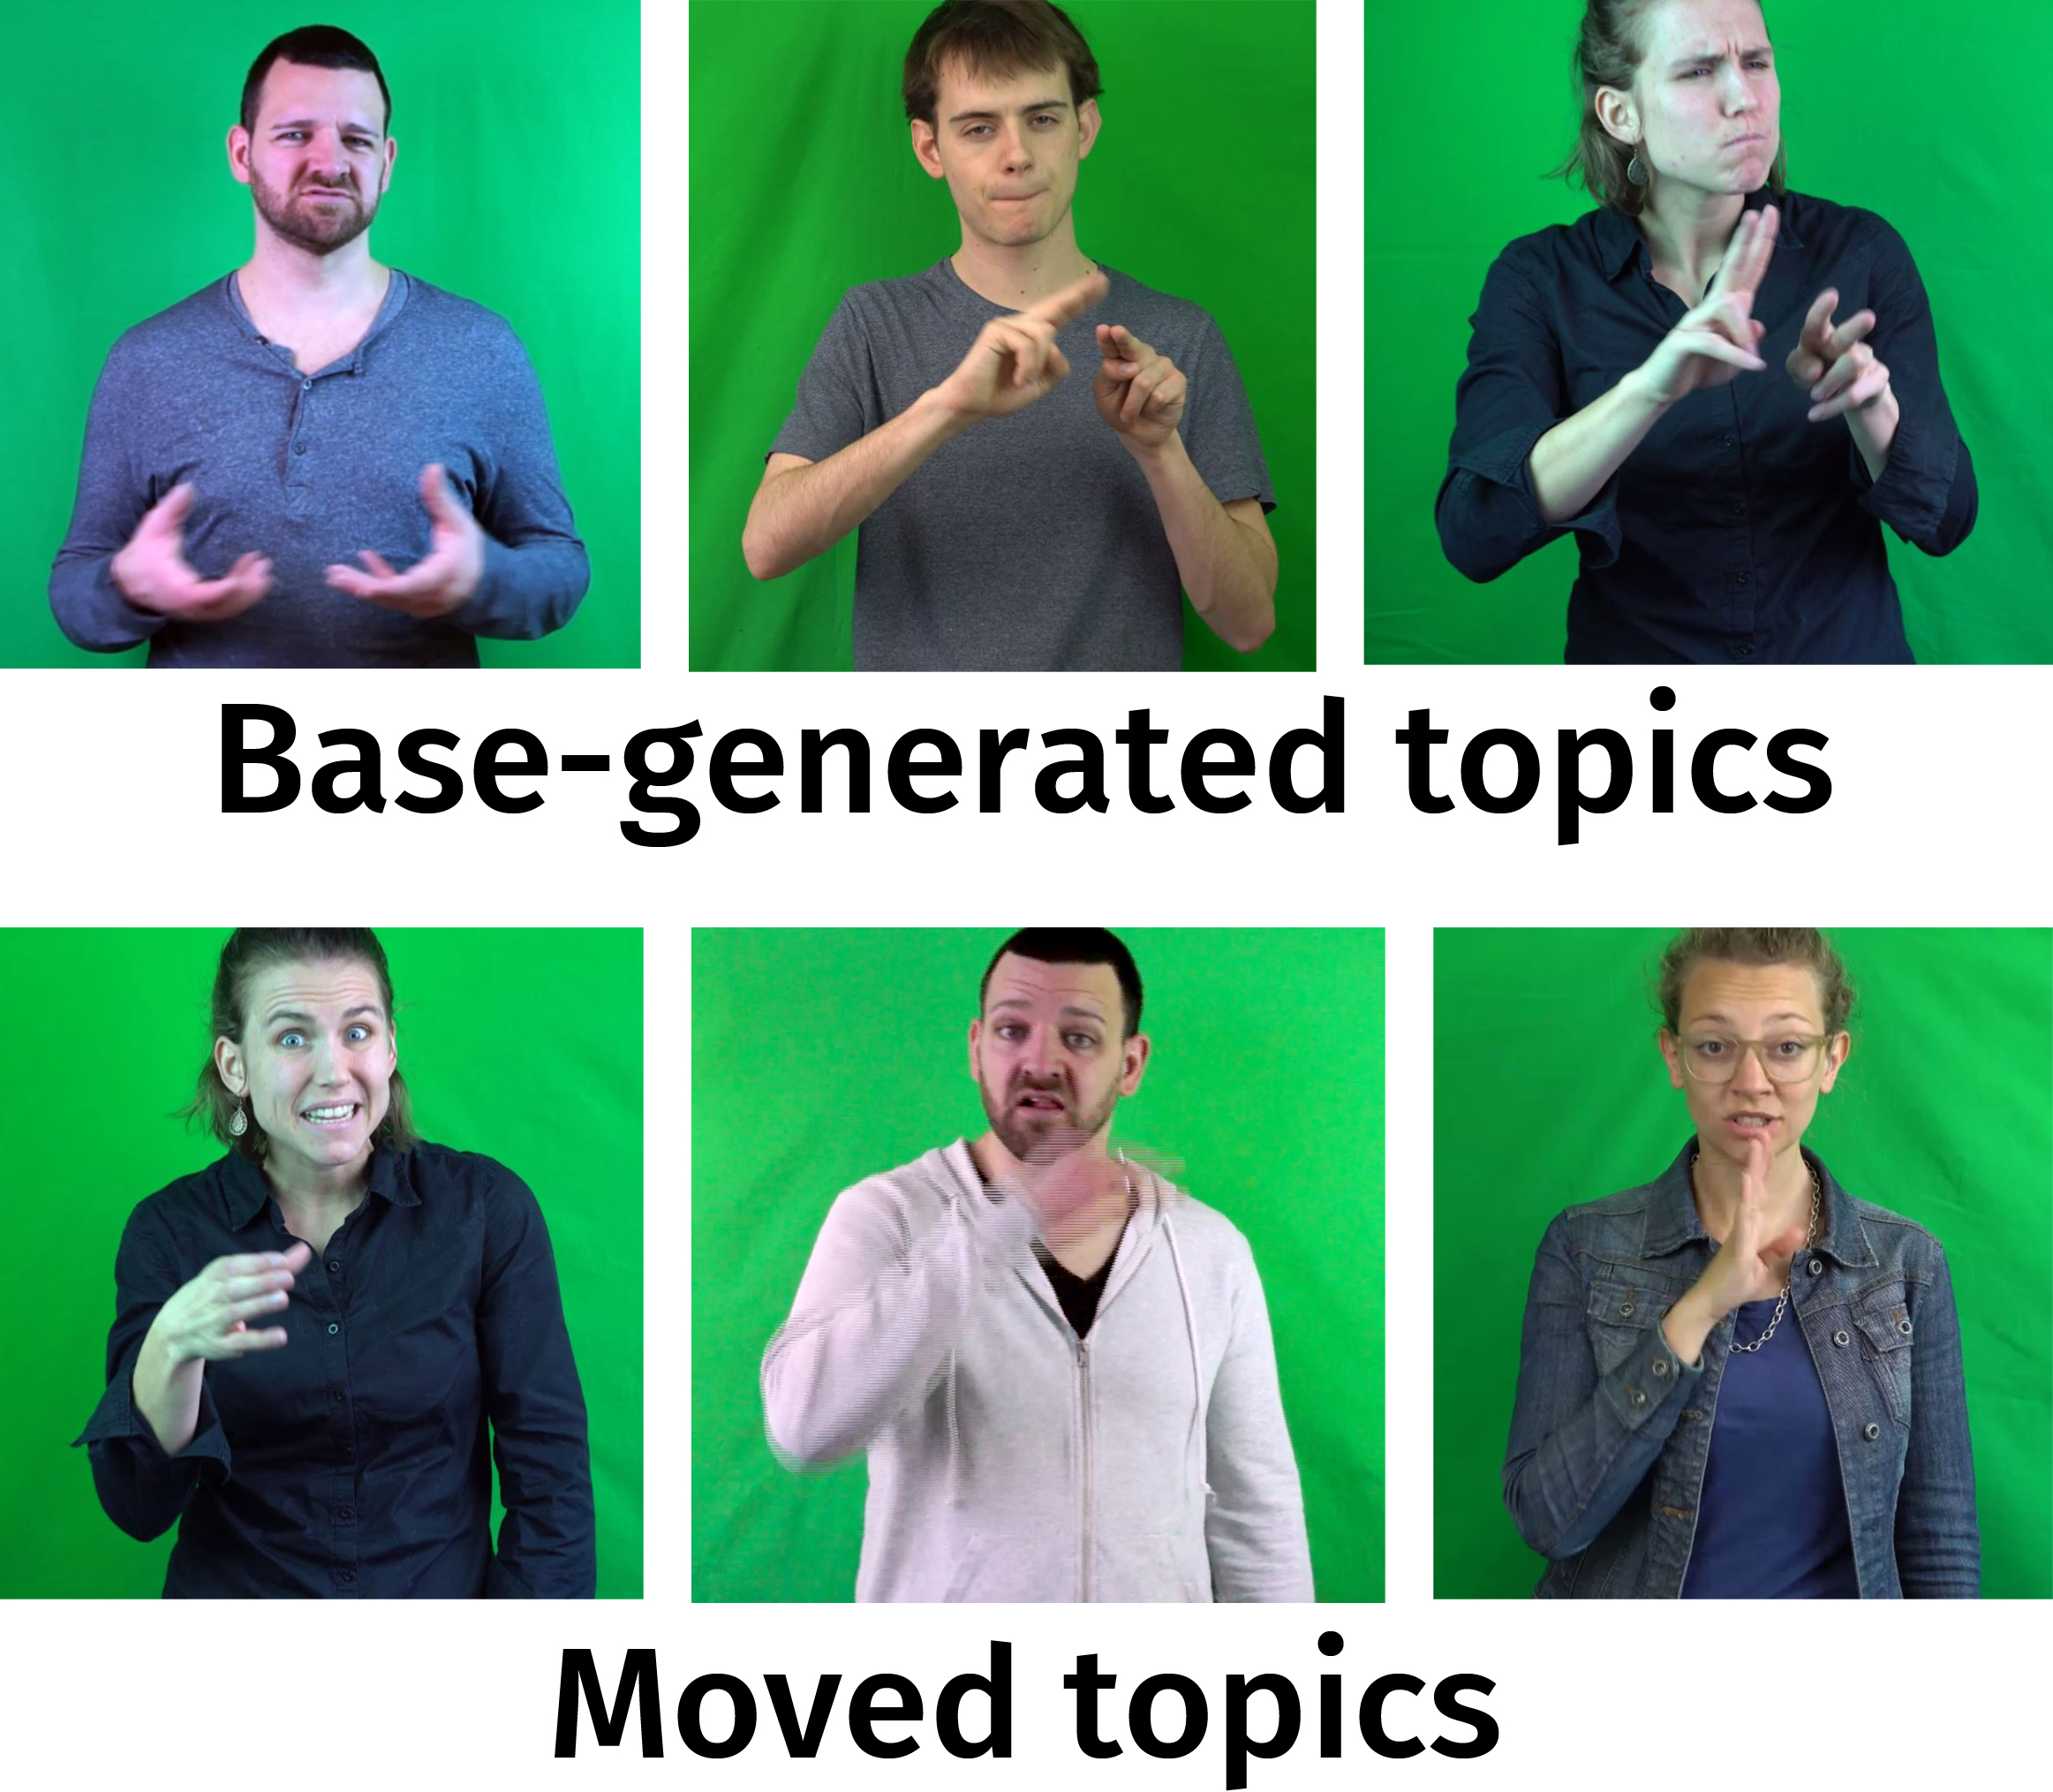
\includegraphics[width=0.9\textwidth]{topicsdgs2.jpg}
	\caption{The non-manual markings used for base-generated (top row) and moved topics (bottom row).}
	\label{topicsindgspicture}
\end{figure}

Topics in DGS, just like in other sign languages (see \citealt{aarons1994aspects} for American Sign Language or \citealt{pfau2008topics} for Sign Language of the Netherlands), can be stacked. It is unclear yet how many topics can be stacked, but due to processing limitations it seems unlikely that there would be more than two or three topics in a sentence. What is clear, however, is that a base-generated topic can be combined with another base-generated topic, as shown in (\ref{topicsindgszwozwoa}).

\begin{exe}
\ex \slg[base-top]{vegetables,} \slg[base-top]{china,} \slg{index\textsubscript{3a} person+++ broccoli eat}
%\ex {\hspace{27pt}{\small base-top}} {\hspace{-1pt}{\small base-top}} {}   \\
%{$\overline{\textrm{\textsc{vegetables}}}$,\textcolor{white}{l}} {$\overline{\textrm{\textsc{china}}}$,}  {\textsc{index}\textsubscript{3a} \textsc{person+++ broccoli eat}}     
\glt `As for vegetables, as for China, people eat broccoli there.' \label{topicsindgszwozwoa} 
\end{exe}

\noindent The example shows that the locative expression \textsc{china} receives the same non-manual marking as the base-generated topic \textsc{vegetables}. This is because \textsc{china} is not an argument of the verb. %Locatives, however, do not need this non-manual marking in any case as I will illustrate in the next subsection. 

This kind of base-generated topic stacking is, however, only possible for constituents that are not arguments of the verb. This means that an argument of the verb cannot receive the `base-top' marking, as shown in (\ref{topicsindgszwozwoamorestackinga}). 

\begin{exe} 
\ex *\slg[base-top]{vegetables,} \slg[base-top]{pepper\textsubscript{\textup{i}},}\textsubscript{\textup{i}} \slg{paul}\textit{t}\textsubscript{i} \slg{like}
%\ex {\hspace{32pt}base-top} {\hspace{6pt}base-top} {}   \\
%{*$\overline{\textrm{\textsc{vegetables,}}}$} {$\overline{\textrm{\textsc{pepper}\textsubscript{i},}}$}  {\textsc{paul} \textit{t}\textsubscript{i} \textsc{like}} 
\glt \textcolor{white}{*}`As for vegetables, as for pepper, Paul likes it.' \label{topicsindgszwozwoamorestackinga}
\end{exe}

\noindent When combining base-generated and moved topics, only one possibility is found. Base-generated topics have to precede moved topics and not the other way around. This is shown by the minimal pair in (\ref{nochanderemoeglichkeiten}).

\begin{exe} 
\ex\label{nochanderemoeglichkeiten}\begin{xlist}
\ex \textcolor{white}{*}\slg[base-top]{vegetables,} \slg[moved-top]{pepper\textsubscript{\textup{i}},} \slg{paul} \textit{t}\textsubscript{i} \slg{like}
%
%\ex {\hspace{32pt}base-top} {\hspace{-1pt}moved-top} {}   \\
%{\textcolor{white}{*}$\overline{\textrm{\textsc{vegetables,}}}$} {\textcolor{white}{l}$\overline{\textrm{\textsc{pepper}\textsubscript{i},}}$}  {\textsc{paul} \textit{t}\textsubscript{i} \textsc{like}} 
\glt \textcolor{white}{*}`As for vegetables, as for pepper, Paul likes it.' \label{nochanderemoeglichkeitena}

\ex *\slg[moved-top]{pepper\textsubscript{\textup{i}},} \slg[base-top]{vegetables,} \slg{paul} \textit{t}\textsubscript{i} \slg{like}
%
%\ex {\hspace{-1pt}moved-top} {\hspace{28pt}base-top}  {}   \\
%{*$\overline{\textrm{\textsc{pepper}\textsubscript{i},}}$} {$\overline{\textrm{\textsc{vegetables,}}}$} {\textsc{paul} \textit{t}\textsubscript{i} \textsc{like}} 
\glt \textcolor{white}{*}`As for pepper, as for vegetables, Paul likes it.' \label{nochanderemoeglichkeitenb}

\end{xlist}
\end{exe}

\noindent The examples in (\ref{nochanderemoeglichkeiten}) are interesting as they show that the base-generated topic seems to be in a structurally higher position than the moved topic. The examples also show that, in line with what was described earlier, base-generated/non-integrated topics are typically used as frame-setting topics (e.\,g., \textsc{vegetables} in (\ref{nochanderemoeglichkeitena})) and moved/integrated topics (e.\,g., \textsc{pepper} in \ref{nochanderemoeglichkeitena}) as aboutness topics. Additionally, the observations are in line with the idea that base-generated frame setters are structurally higher than moved aboutness topics. 


%\clearpage

\begin{digression}{Topicalization in event conditionals}{}
\noindent It has been noted in the literature than many languages, including English, do not allow topicalization in adverbial clauses. A prime example are event conditionals, cf. (\ref{eventconditionalhaegemann}) from \citet[332]{haegeman2003conditional}.

\begin{exe}
\ex *If these final exams you don't pass you won't get a degree. \label{eventconditionalhaegemann}
\end{exe}

\noindent That topicalization is not possible in event conditionals is usually explained by assuming that they exhibit a deficient left periphery \citep{haegeman2003conditional, haegeman2004topicalization} (but see \citealt{haegeman2013syntax} for an alternative account). However, in some languages, topicalization of this sort is possible. This is, for example, the case with Bavarian Extraction shown in (\ref{bavarianextraction}).

\begin{exe}
\ex Bavarian \citep[232]{grewendorf2015bavarian} \\ \gll {[\textit{De}} {\textit{Mass}]\textsubscript{i}} {\textit{wenn}} {\textit{i}} {t\textsubscript{i}} {\textit{no}} {\textit{drink},} {\textit{bin}} {\textit{i}} {\textit{bsuffa}}   \\
{this} {liter} {if} {i} {} {still} {drink} {am} {I} {drunk} \\
\trans `If I drink this Mass, I will be drunk.'   \label{bavarianextraction}
\end{exe}

\noindent A similar observation can be made with regard to DGS (for similar observations regarding Sign Language of the Netherlands, see \citealt{pfau2008topics}). The example in (\ref{bavarianextractiondgsa}) shows a regular DGS event conditional. The example in (\ref{bavarianextractiondgsb}) illustrates that topicalization is, similar to Bavarian, possible. Note that the manual conditional marker \textsc{if} is optional in DGS. 

\begin{exe}
\ex\begin{xlist}  \label{bavarianextractiondgs}
\ex \slg[conditional]{(if) index_2 exam \slg[\textup{hs}]{pass}} \slg[hs]{can-neg} \slg{apprenticeship}\\
`If you don't pass the exam you won't be able to do an apprenticeship.' \label{bavarianextractiondgsa}
\ex \slg[move-top]{exam_{\textup{i}}} \slg[conditional]{(if) index_2 \textup{t}_{\textup{i}} \slg[\textup{hs}]{pass}} \slg[hs]{can-neg} \slg{apprenticeship}\\
`If you don't pass the exam you won't be able to do an apprenticeship.' \label{bavarianextractiondgsb}
\end{xlist}
\end{exe}

\noindent Is is interesting to note, however, that the left periphery of event conditionals in DGS still is truncated. This can be seen by the fact that \textit{wh}-movement is blocked in conditionals in DGS and \textit{wh}-phrases need to stay \textit{in-situ}.




%\begin{exe}
%\ex 
%\glll   {${\hspace{77}\underline{\textrm{\quad hn}}}$} \\
%{\hspace{77pt}cond}  {\hspace{10}hs} \\
%{$\overline{\textrm{\textsc{index}\textsubscript{2} \textsc{exam pass}}}$} {$\overline{\textrm{\textsc{can}}}$}  { \textsc{apprenticeship}}\\
%\glt \textcolor{white}{\%}`If you don't pass the exam you won't be able to do an apprenticeship.' \label{ex:topicconditionaldgsa}
%\end{exe}
%

\end{digression}

\is{topic|)}

\section{Foci}\label{generalfocussection}
\is{focus|(}
\subsection{General overview}
\label{finersplitsfocus}
\is{focus|(}
The notion of topic has to be strictly kept apart from the notion of focus, as focus, in contrast to (non-contrastive) topics, can affect truth conditions. This can be shown, for example, with focus particles like English \textit{only}. In a sentence with the focus particle \textit{only}, as in (\ref{focustrughcond}), one constituent needs to be associated with focus. In English, this is done by pitch accent, usually highlighted using small caps. Depending on which constituent is focused, the sentence is assigned different truth-conditions as can be seen from the paraphrases. %Small caps indicate pitch accent.   %While the choice of the topic does not affect truth conditions, the choice of the focus can. 



\begin{exe}
\ex\label{focustrughcond}
\begin{xlist} 
\ex John only saw $[$\textsubscript{Focus} the \textsc{play}$]$ yesterday. \\
`There is nothing apart from the play that Paul saw yesterday.'\label{ex:focustrughconda}
\ex John only saw the play $[$\textsubscript{Focus} \textsc{yes}terday$]$. \\
`There is no other day apart from yesterday on which Paul saw the play.'\label{ex:focustrughcondb}
\end{xlist}
\end{exe}

\noindent The minimal pair in (\ref{focustrughcond}) illustrates that the choice of which constituent is focused can lead to truth value changes. In this case, this is because what is focused is interpreted as relevant while other possible alternatives are excluded: ``Focus indicates the presence of alternatives that are relevant for the interpretation of linguistic expressions'' \citep[18]{krifka2007basic}. This means that the example in (\ref{ex:focustrughconda}) will get the interpretation that John saw nothing else than the play yesterday and no other alternatives (as, for example, some specific movie that was mentioned in the context). Similarly, (\ref{ex:focustrughcondb}) will get the interpretation that John saw the play on no other day than yesterday and not on any alternative day. 

While the term `topic', loosely, refers to what a sentence is about, the term `focus' refers, loosely, to new information in a sentence. In example (\ref{focustrughcond}) above, the speaker assumed that the hearer had the wrong alternatives in mind and added the correct alternative (while excluding the wrong alternatives at the same time) as new information. 

\subsubsection{Broadening the picture: two definitions of focus}
Of course, focus is not restricted to \textit{only} foci and a broader picture is needed. Focus is, for example, also used in answers to questions, as the answer to a question has to be, by definition, new to the hearer. Following \citet{rooth1996focus}, we can say that the focus in an answer to an alternative question correlates to the position of the disjoint alternatives. For \textit{wh}-questions, focus correlates with the position of the \textit{wh}-element. This is shown in (\ref{rooth1996}), from \citet{rooth1996focus}. There are two questions in the illustration, an alternative question (on the left) and a \textit{wh}-question (on the right). Although both answers at the bottom of the illustration are made up of the same lexical material they cannot be used interchangeably. The answers corresponding to the questions of which they would be considered appropriate are linked by solid lines, the dashed lines show inappropriate question-answer pairs. 

\begin{exe}
\ex\label{rooth1996} 
%\begin{figure}
%\centering
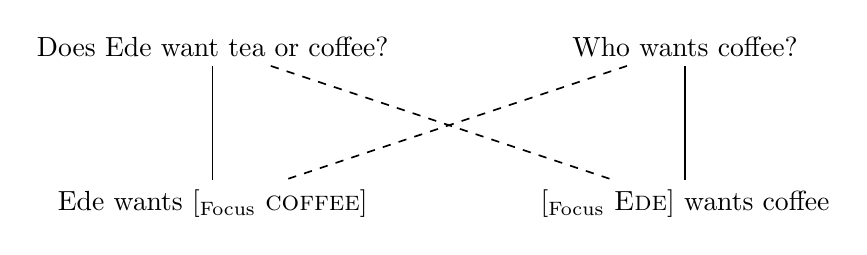
\begin{tikzpicture}[baseline={([yshift={-2.3ex}]current bounding box.north)}, scale=1.00]
\tikzset{level 1+/.style={sibling distance=2\baselineskip}}
%\Tree [.DP [.D the ] [.NP man ]]
\node (a) at (0,0) {Does Ede want tea or coffee?} ;
\node (b) at (6,0) {Who wants coffee?} ;

\node (c) at (0,-2) {Ede wants $[$\textsubscript{Focus} \textsc{coffee}$]$} ;
\node (d) at (6,-2) {$[$\textsubscript{Focus} \textsc{Ede}$]$ wants coffee} ;

\draw[semithick, -] (b) to (d);
\draw[semithick, -] (a) to (c);
\draw[semithick, -,dashed] (b) to (c);
\draw[semithick, -,dashed] (a) to (d);
%\draw[help lines] (-4,-4) grid (4,4)
\end{tikzpicture}
%\caption{Question-answer congruence for focus (after Rooth 1996).}
%\end{figure}
\end{exe}

\noindent What (\ref{rooth1996}) shows is that when a speaker asks if Ede wants coffee or tea, the fact that Ede wants something is already established. What the speaker consequently assumes is that what Ede wants to drink will be new to the asker and is thus in focus. It would not be felicitous to focus \textit{Ede}, since the fact that he wants something is already known. Similarly, when it is asked who it is that wants coffee, the newsworthy information is the name of the referent that wants to drink something. 

Note that we have two definitions of focus now. One that is about alternatives and one that is about new information. So while, for example, \citet[18]{krifka2007basic} states that focus is the indication of alternatives relevant to the interpretation, \citet[1876]{hinterwimmer2011formation} defines focus as that ``part of the sentence that conveys the information the speaker wishes to represent most prominently and onto which s/he wants to draw the hearer's attention.'' Both definitions do not contradict each other. Focus does evoke alternatives that are viewed as relevant to the speaker, the alternative that is highlighted is highlighted because the speaker assumes that this alternative is new to the hearer: to highlight something always means to highlight something with respect to something else (and these are the alternatives).\footnote{ To be more precise, it is not the alternative itself that needs to be new to the hearer but the relation of the alternative to the rest of the proposition. Consider the example in (\ref{kissmotherrelation}), from \citet[55]{rochemont2016givenness}. From the example it becomes clear that \textit{John} can be focused, although it is already given in the context.

\begin{exe}
\ex A: Who did John's mother kiss? \\
B: She kissed \textsc{John}. \label{kissmotherrelation}
\end{exe}

\noindent This is possible as the new information is the relation John has with the kissing event.

}

\subsubsection{Focus and presupposition versus topic and comment}
Everything that is not focused in a sentence is called the `presupposition' or the `background'. The proposal to divide focus and background goes back to \citet{jackendoff1972semantic} who defines the focus of a sentence as ``the information in the sentence that is assumed by the speaker not to be shared by him and the hearer'' and presupposition respectively as ``the information in the sentence that is assumed by the speaker to be shared by him and the hearer'' \citep[230]{jackendoff1972semantic}.\footnote{ The knowledge that is shared by the interlocutors is usually called the `common ground' \citep{stalnaker1978assertion}.}

Although a sentence can be split up into a topic and a comment part, with the topic referring to old information and although the focus refers to new information, focus and comment are not the same. This is because the terms refer to different levels of information structure. This can be explained best by means of an example. In many cases, the topic of a sentence and its presupposition on the one hand, and the focus and the comment on the other hand, coincide. This is illustrated in the example dialogue in (\ref{topicfocusdistincitona}), taken from \citet[467]{vallduvi1996linguistic}.

\begin{exe}
\ex\label{topicfocusdistincitona}
A: What about John? What does he do? \\
B: John drinks \textsc{beer}.
\end{exe}

\noindent The information structure of Bob's answer to Alice's question can be represented in terms of topic and comment (\ref{ex:topicfocusdistincitonba}) and in terms of focus and presupposition (\ref{ex:topicfocusdistincitonbb}). From the two representations it looks as if we could conflate the four notions and equate topic with presupposition and focus with comment.

\begin{exe}
\ex\label{topicfocusdistincitonb}\begin{xlist} 
\ex $[$\textsubscript{Topic} John$]$ $[$\textsubscript{Comment} drinks \textsc{beer}$]$ \label{ex:topicfocusdistincitonba}
\ex $[$\textsubscript{Presupposition} John$]$ $[$\textsubscript{Focus} drinks \textsc{beer}$]$ \label{ex:topicfocusdistincitonbb}
\end{xlist}
\end{exe}

\noindent There are, however, examples that show that this is not always the case. The information structure of Bob's answer in (\ref{topicfocusdistincitona}) is mainly determined by Alice's question. As her first question is about John, John has to be given. Her second question is about the action John performs. What exactly this action is, is left open. If we change Alice's question and make it more specific, the difference between topic and presupposition as well as the difference between focus and comment is more obvious, as shown in the example dialogue in (\ref{topicfocusdistincitonc}), again taken from \citet[468]{vallduvi1996linguistic}.

\begin{exe}
\ex\label{topicfocusdistincitonc}
A: What about John? What does he drink? \\
B: John drinks \textsc{beer}.
\end{exe}

\noindent Note that what changed in the dialogue in (\ref{topicfocusdistincitonc}) is not Bob's answer, but only Alice's question. She is now asking something more specific, namely, what John is drinking. Therefore, the drinking is already given and therefore cannot be in the focus of Bob's answer, but it is part of the presupposition. Additionally, John is also in the presupposition, since Alice also asked about John. Nevertheless, John is also what Bob's sentence is about, hence John is also the topic of the sentence. The only thing left now is the beer. The beer is the only new information that is provided by Bob, so it is the focus. We arrive at the following structure:

\begin{exe}
\ex\label{topicfocusdistincitond}\begin{xlist} 
\ex $[$\textsubscript{Topic} John$]$ $[$\textsubscript{Comment} drinks \textsc{beer}$]$ \label{ex:topicfocusdistincitonbaa}
\ex $[$\textsubscript{Presupposition} John drinks$]$ $[$\textsubscript{Focus} \textsc{beer}$]$ \label{ex:topicfocusdistincitonbbb}
\end{xlist}
\end{exe}

\noindent The representation in (\ref{ex:topicfocusdistincitonbaa}) shows that the topic-comment structure has not changed. Bob's answer is still a sentence about John, about whom it is commented that he drinks beer. What has changed, however, is the focus-presupposition structure. That John drinks something is presupposed by Alice's question. What is new, i.\,e., what is the focus of the sentence, is that it is beer that he drinks. 

\subsubsection{The syntax of focus: two structural positions}
While there are (at least) two topic positions in the CP area, as discussed in the previous section, there is only one focus position. Nevertheless, two types of focus with two different structural positions can be differentiated. These two types are called contrastive (or: identificational) and information focus (see \citealt{kiss1981structural}). Contrastive focus is exhaustive, i.\,e., it selects an item from a larger set of items and is used for contrasts and corrections. Information focus needs not be exhaustive. It is used as an answer to a \textit{wh}-question as was already introduced on page \pageref{rooth1996} (see the example in (\ref{rooth1996})). 

Languages use different strategies to mark constrastive focus. Some languages, for example, English, use cleft structures and intonational means to mark contrastive focus, as shown in (\ref{constrativefocusexample}). Other languages, for example Bulgarian, do not only prepose topics, but also foci -- without using a cleft strategy. In cases in which a topicalized and a focalized element occur in one clause, we find the topic preceding the focus, as shown in the Bulgarian example from \citet[72]{van1995focus} in (\ref{constrativefocusexamplebulgarian}).\footnote{ An interesting feature in Bulgarian is that the focus head is realized overtly with the focus marker \textit{li}. }

\begin{exe}
\ex A: Why did Sarah buy so much beer?\\
B: It was \textsc{Lorenz} who bought the beer. \label{constrativefocusexample}
\end{exe}

\begin{exe}
\ex Bulgarian \citep[72]{van1995focus} \\ \gll {\textit{Filma}} {\textit{Marija}} {\textit{li}} {\textit{gleda?}}  \\
{film} {Marija} {\textsc{foc}} {watch} \\
\trans `As for the film, it is Marija who is watching it?'   \label{constrativefocusexamplebulgarian}
\end{exe}

\noindent From data like the Bulgarian one, it was argued that these two types of focus are located in two different structural positions: a high, CP-internal position for contrastive focus and a low, IP-internal position for (new) information focus (see, for example, \citealt{beninca2001position}; \citealt{benincapol2004topic}; \citealt{belletti2004aspects}; \citealt{belletti2003i}).

\begin{table}[t]
\centering

\begin{tabular}{p{2.5cm}p{4.5cm}p{4.5cm}}
\lsptoprule
 & \textsc{Contrastive focus} & \textsc{Information focus} \\
\midrule
\rowcolor[gray]{.9}
Usage & Exhaustive identification & Marking information as being non-presupposed \\
Behavior & Optional & Present in every utterance \\
\rowcolor[gray]{.9}
Movement & Yes & No \\
%\rowcolor[gray]{.9}
%Binding effects & Yes & No \\
%Island sensitive & Yes & No \\
%\rowcolor[gray]{.9}
%Intonational break & No & Yes \\
\lspbottomrule
\end{tabular}
\caption{Some differences between contrastive and information focus (based on \citealt{kiss1998identificational})}
\label{ldhtdiff}
\end{table}








% 

\is{focus|)}


\subsection{Foci in sign languages}
While research on sign languages has shown, mainly for American Sign Language, that topics appear in a clause-initial position, the position for foci seems to be a different one. The position for focused elements (or more general: new information) in American Sign Language is clause-final rather than clause-initial \citep{wilbur1991intonation, wilbur1994foregrounding, wilbur1996evidence, wilbur1997prosodic}. Similar observations have been made for other sign languages, including, for example, Brazilian Sign Language \citep{de1999phrase} and Sign Language of the Netherlands \citep{crasbornkoijiros2012}. 

\citet[92]{wilbur1997prosodic} illustrates clause-final focus in American Sign Language with modals which occur preverbally in the language when unfocused. When focused, however, they appear in a clause-final position, as shown in (\ref{focusedmodalronnie}).

\begin{exe}
\ex American Sign Language \citep[92]{wilbur1997prosodic} \\ % {\hspace{105pt}br}   \\
{\textsc{\dots\ but stay home all-day everyday can't}}
\glt `\dots\ but I \textsc{can't} stay home all day everyday.' \label{focusedmodalronnie}
\end{exe}

\noindent Three analyses were offered for this clause-final focus position: leftward movement, rightward movement, and \is{focus doubling} doubling with deletion: \citet{wilbur1997prosodic}, for example, suggests that non-focus material is preposed, i.\,e., moved to the left. Others, e.\,g., \citet{petronio1993clause}, have suggested the focused elements are moved to the right, maybe involving an additional step of doubling the focused element with subsequent deletion of the clause-internal copy. It is not clear yet which of these analyses should be preferred.  

Another\is{focus doubling} example illustrating that focused elements appear in a clause-final position in American Sign Language are doubling constructions. In American Sign Language, as in many other sign languages, several elements that originally appear in a clause-internal position can be doubled in a clause-final position. This is, for example, possible with modals as shown in (\ref{doublingaslmodals}) from \citet[135]{petronio1993clause}.\footnote{ Other elements that can be doubled in American Sign Language include quantifiers, negatives, and \textit{wh}-signs \citep{petronio1993clause}.}

\begin{exe}
\ex \slg[pol]{ann will leave will}
%\ex {\hspace{105pt}pol}   \\
%{$\overline{\textrm{\textsc{ann will leave will}}}$} 
\glt `Will Ann leave?' \label{doublingaslmodals}
\end{exe}

\noindent The second, `doubled' modal in examples like the one in (\ref{doublingaslmodals}) usually receives focus given that it is prosodically prominent. In some sign languages, for example in Brazilian Sign Language, the doubles receive head nods \citep{de1999phrase}. The claim that doubling is related to focus is supported by the fact that there can only be one double per clause. Additionally, an element, such as a modal, cannot be doubled in a \textit{wh}-question. As \textit{wh}-phrases are thought to be located in FocP (or at least to move through FocP), it is reasonable to assume that the clause-final double is located in FocP. 

It is usually argued that the double is located in the head of the focus phrase as only single signs, i.\,e., heads, can be doubled. We could thus assume either a right-headed FocP or a left-headed and left-branching FocP with an additional remnant movement step that moves the clause to the left of the Foc\textdegree\ (in the specifier of the FocP).  

While doubling only involves heads, there are other constructions in which phrases occur in a clause-final position. \label{pseudocleeeeefts}A common strategy of overt syntactic focusing in American Sign Language are pseudo-clefts. This construction, traditionally called `rhetorical question structure', is illustrated in (\ref{wilburrqanp}).

\begin{exe}
\ex American Sign Language \citep[92]{wilbur1997prosodic} \\ \slg[br]{find\#out what,} \slg{stay home can't}
%\ex {\hspace{82pt}br} {}   \\
%{$\overline{\textrm{\textsc{find\#out what}}}$,} {\textsc{stay home can't}}
\glt `What I discovered is that \textit{I can't stay home}.' \label{wilburrqanp}
\end{exe}

\noindent \citet{wilbur1997prosodic} argues that in these constructions, the first part of pseudo-cleft structures, as in (\ref{wilburrqanp}), which are accompanied by a brow raise, is the non-focused part consisting of an open proposition and the second part of the structure represents the focused material (see also \citealt{wilbur1994foregrounding, wilbur1996evidence}). An alternative account on this construction is presented by \citet{caponigro2011ask} who, similar to \citet{wilbur1996evidence}, assume that the structure forms a syntactic and semantic unit. Their account, however, is different from \citeauthor{wilbur1996evidence}'s as they argue that the question constituent receiving the brow raise is an embedded interrogative clause and the answer constituent is an embedded declarative clause with the whole structure being a declarative clause. 

Concerning the non-manual markers used for focus marking, the literature mainly reports head nods and raised eyebrows  as well as shoulder movements. The shoulders were found to play a role, for example, in contrastive focus in American Sign Language \citep{wilbur1999syntactic} as well as in Sign Language of the Netherlands \citep{crasborn2013phonology}.

\subsection{Foci in DGS}
In this section, I will give a brief overview of the focusing strategies used in DGS. In line with the literature, I will show that information focus mainly stays unmarked. As in other sign languages, DGS exhibits focus doubling and pseudo-clefts which are marked in a similar manner as in American Sign Language. Concerning contrastive focus I will show that the non-manual marking which is used is subject to dialectal variation as signers from Baden-Württemberg and signers from Bavaria use different strategies. Finally, I will briefly discuss the role of signing space and shoulder positions in contrastive focus. For the use of focus particles in DGS, which will not be discussed here, I refer the reader to \citet{herrmann2013modal}.

\subsubsection{Information focus}
With information focus\is{information focus} we do not find any reordering (i.\,e., movement) of manual constituents. On the whole, it information focus is usually left unmarked (see also \citealt{waleschkowski2009}). When it is marked, wide-open eyes, a short eyebrow raise, and a slight downward movement of the head or a head-nod on the focused constituent can be observed (see also \citealt[396]{happ2014vork}). This is shown in the example in (\ref{ex:informationfocusnewexample}).

\begin{exe}
\ex\label{ex:informationfocusnewexample}
A: Who did you meet yesterday?\\
\textcolor{white}{B: }\slg{yesterday} \slg[foc]{paul} \slg{meet}
%{} {\textcolor{white}{B: \textsc{yesterdayml}}foc} {}   \\
%{B: \textsc{yesterday}} {$\overline{\textrm{\textsc{paul}}}$} {\textsc{meet}}      
\glt \textcolor{white}{B: }`I met \textsc{Paul} yesterday.' 
\end{exe}

\noindent Wide information focus can also be marked by wide-open eyes and raised eyebrows spreading over the whole clause. This is illustrated in (\ref{ex:wideinformatiofocus}) -- although in most cases, wide focus stays unmarked. %However wide information focus mainly stays unmarked.

\begin{exe}
%\ex What happend?\label{ex:informationfocusdgspapaspyrou}\begin{xlist} 
\ex
A: What happened? \\
B: \slg[foc]{poss\textsubscript{1} beer fall-down}
%
%{\hspace{129pt}foc}    \\
%%{\hspace{\fill}foc} \\
%{B: $\overline{\textrm{\textsc{\textsc{poss}}\textsubscript{1} \textsc{beer fall-down}}}$}  
\glt \textcolor{white}{B: }`My beer fell down.' \label{ex:wideinformatiofocus}

\end{exe}

\noindent Taken together, if information focus is marked at all, it is marked by wide-open eyes and slightly raised eyebrows. 



\subsubsection{Focus doubling}\is{modal doubling|see{focus doubling}}\is{focus doubling}\is{doubling|see{focus doubling}}
As described for American Sign Language, several elements can undergo doubling in DGS, including \textit{wh}-signs (see Section \ref{whinterrogativedgs}), pronouns (see Section \ref{polarinterrogativesdgs}), and modals verbs (see Section \ref{modaldoubling}). As in other sign languages, the items undergoing doubling are heads and not full phrases (but see Section \ref{whinterrogativedgs} for evidence that this is different for \textit{wh}-doubling). In many (but not all) cases, the clause-final double receives stress, as shown in (\ref{modaldoublingdgsexample}). 

\begin{exe}
\ex \slg{paul can swim} \slg[foc]{can}
%{} {\hspace{97pt}foc}    \\
%{\textsc{paul can swim}} {$\overline{\textrm{\textsc{can}}}$}
\glt `Paul \textsc{can} swim.' \label{modaldoublingdgsexample}
\end{exe}

\noindent If we assume that the double is hosted in a head we could either assume FocP to be right-headed or that the non-doubled lexical material has moved to a left-branching specifier -- probably SpecFocP. 



\subsubsection{Pseudo-clefts}\is{pseudo-cleft}\is{wh-cleft@\textit{wh}-cleft|see{pseudo-cleft}}\is{cleft|see{pseudo-cleft}}
Similar to what was described for American Sign Language, pseudo-clefts are possible in DGS (cf. \citealt[397]{happ2014vork}). As with American Sign Language, the non-focused material can receive a brow-raise (glossed `cleft' in the example). The focused phrase in the clause-final position can receive non-manual focus marking that can be either a brow-raise or a backwards head tilt, sometimes accompanied by a nod. An example is given in (\ref{whcleft}).% which is additionally depicted in Figure \ref{pseudocleft}.

\begin{exe}
\ex \slg[cleft]{paul break what} \slg[(foc)]{vase}
%\ex {\hspace{80pt}cleft} {\hspace{14pt}foc}   \\
%{$\overline{\textrm{\textsc{paul break what}}}$,} {$\overline{\textrm{\textsc{vase}}}$}
\glt `What Paul broke was \textsc{the vase}.' \label{whcleft}
\end{exe}

\noindent According to \citet[397]{happ2014vork} the first part of cleft-structures like the one in (\ref{whcleft}) receive a topic-marking, i.\,e., raised eyebrows. This is in line with my own observations. Similar to the description in \citet[397]{happ2014vork}, the focus marking can be, and usually is, absent. Both possibilities are depicted in Figure \ref{pseudocleft}. In the top example the focus marking on \textsc{beer} is missing, in the bottom example, the focus marking is present (an additional brow-raise). The premise for the focus marking to be present seems to be that it marks new or unexpected information. While the top example would be felicitous at the beginning of a talk (when everyone knows that a talk about beer will follow), the second example was elicited in a context in which the signer was reporting that he will visit a talk about beer (`I'm going to a talk. The topic of the talk is beer').\footnote{ This difference is also mirrored in constituent order in the examples.} Pseudo-clefts in DGS need further attention in the future. In my mind, it is not clear yet if they are really best analyzed as focus structures, but as topic-comment structures as similar constructions in the spoken language research tradition were indeed analyzed this way (e.\,g., \citealt{prince1978,gast2014}; see also \citealt{caponigro2011ask} for a similar point for American Sign Language).

\begin{figure}[bt]
\centering
	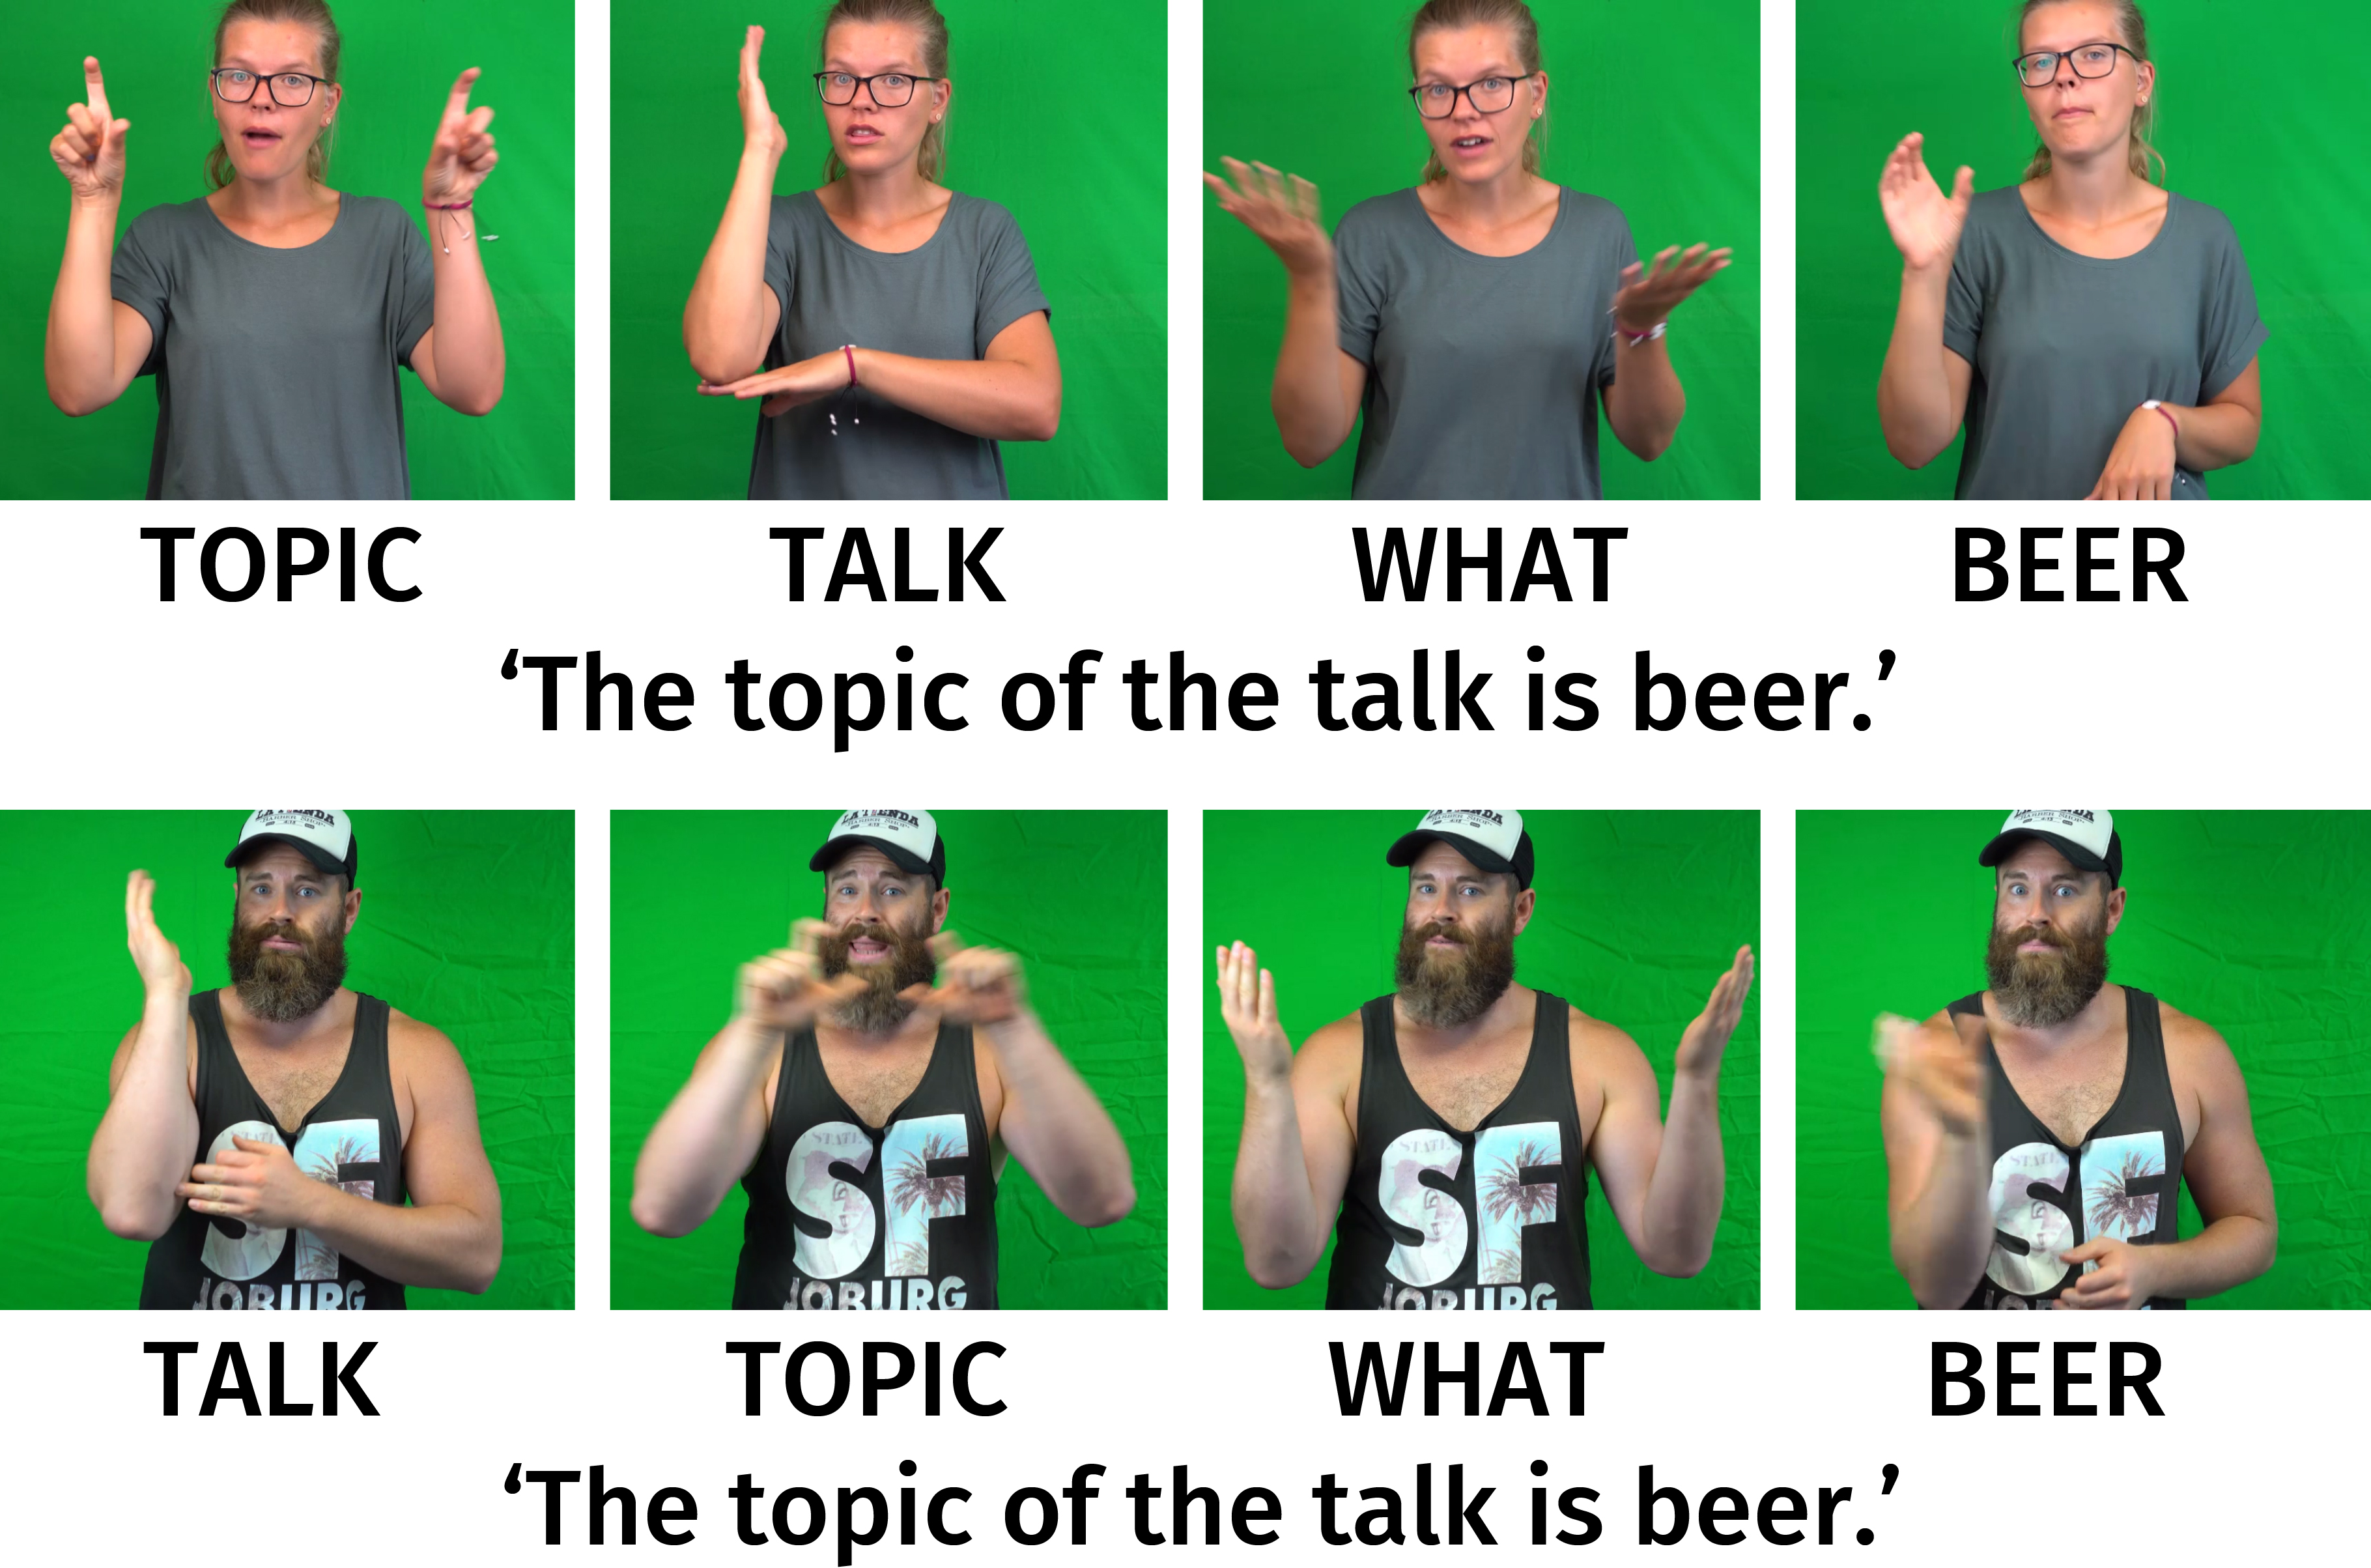
\includegraphics[width=1.0\textwidth]{pseudoclefttwo.jpg}
	\caption{Two pseudo-clefts: one without and one with focus marking.}
	\label{pseudocleft}
\end{figure}

\subsubsection{Contrastive focus}\label{contrastivefocussubection}
Previous\is{contrastive focus} research on focus in German Sign Language has noted that contrastive focus is marked mainly by head nods \citep{waleschkowski2009}. \citet[402--403]{happ2014vork} also report that the non-manual marking for information and contrastive focus is the same and thus is achieved by nods (except for pseudo-clefts which are described above). This only partly matches with my own observations. 

With contrastive focus I found a unique bundle of non-manual markers that consist either of the head tilted backward and raised eyebrows or of a forward head-bow or chin-down with furrowed brows. The question of which of these non-manuals are used is subject to dialectal variation. While signers from Baden-Württemberg systematically used head-tilts and eyebrow-raises, the chin-down pattern was used by the Bavarian signers. This is shown in Figure \ref{contrastivefocus}. In both cases, the non-manuals accompany the whole constituent being contrasted.

\begin{figure}[bt]
\centering
	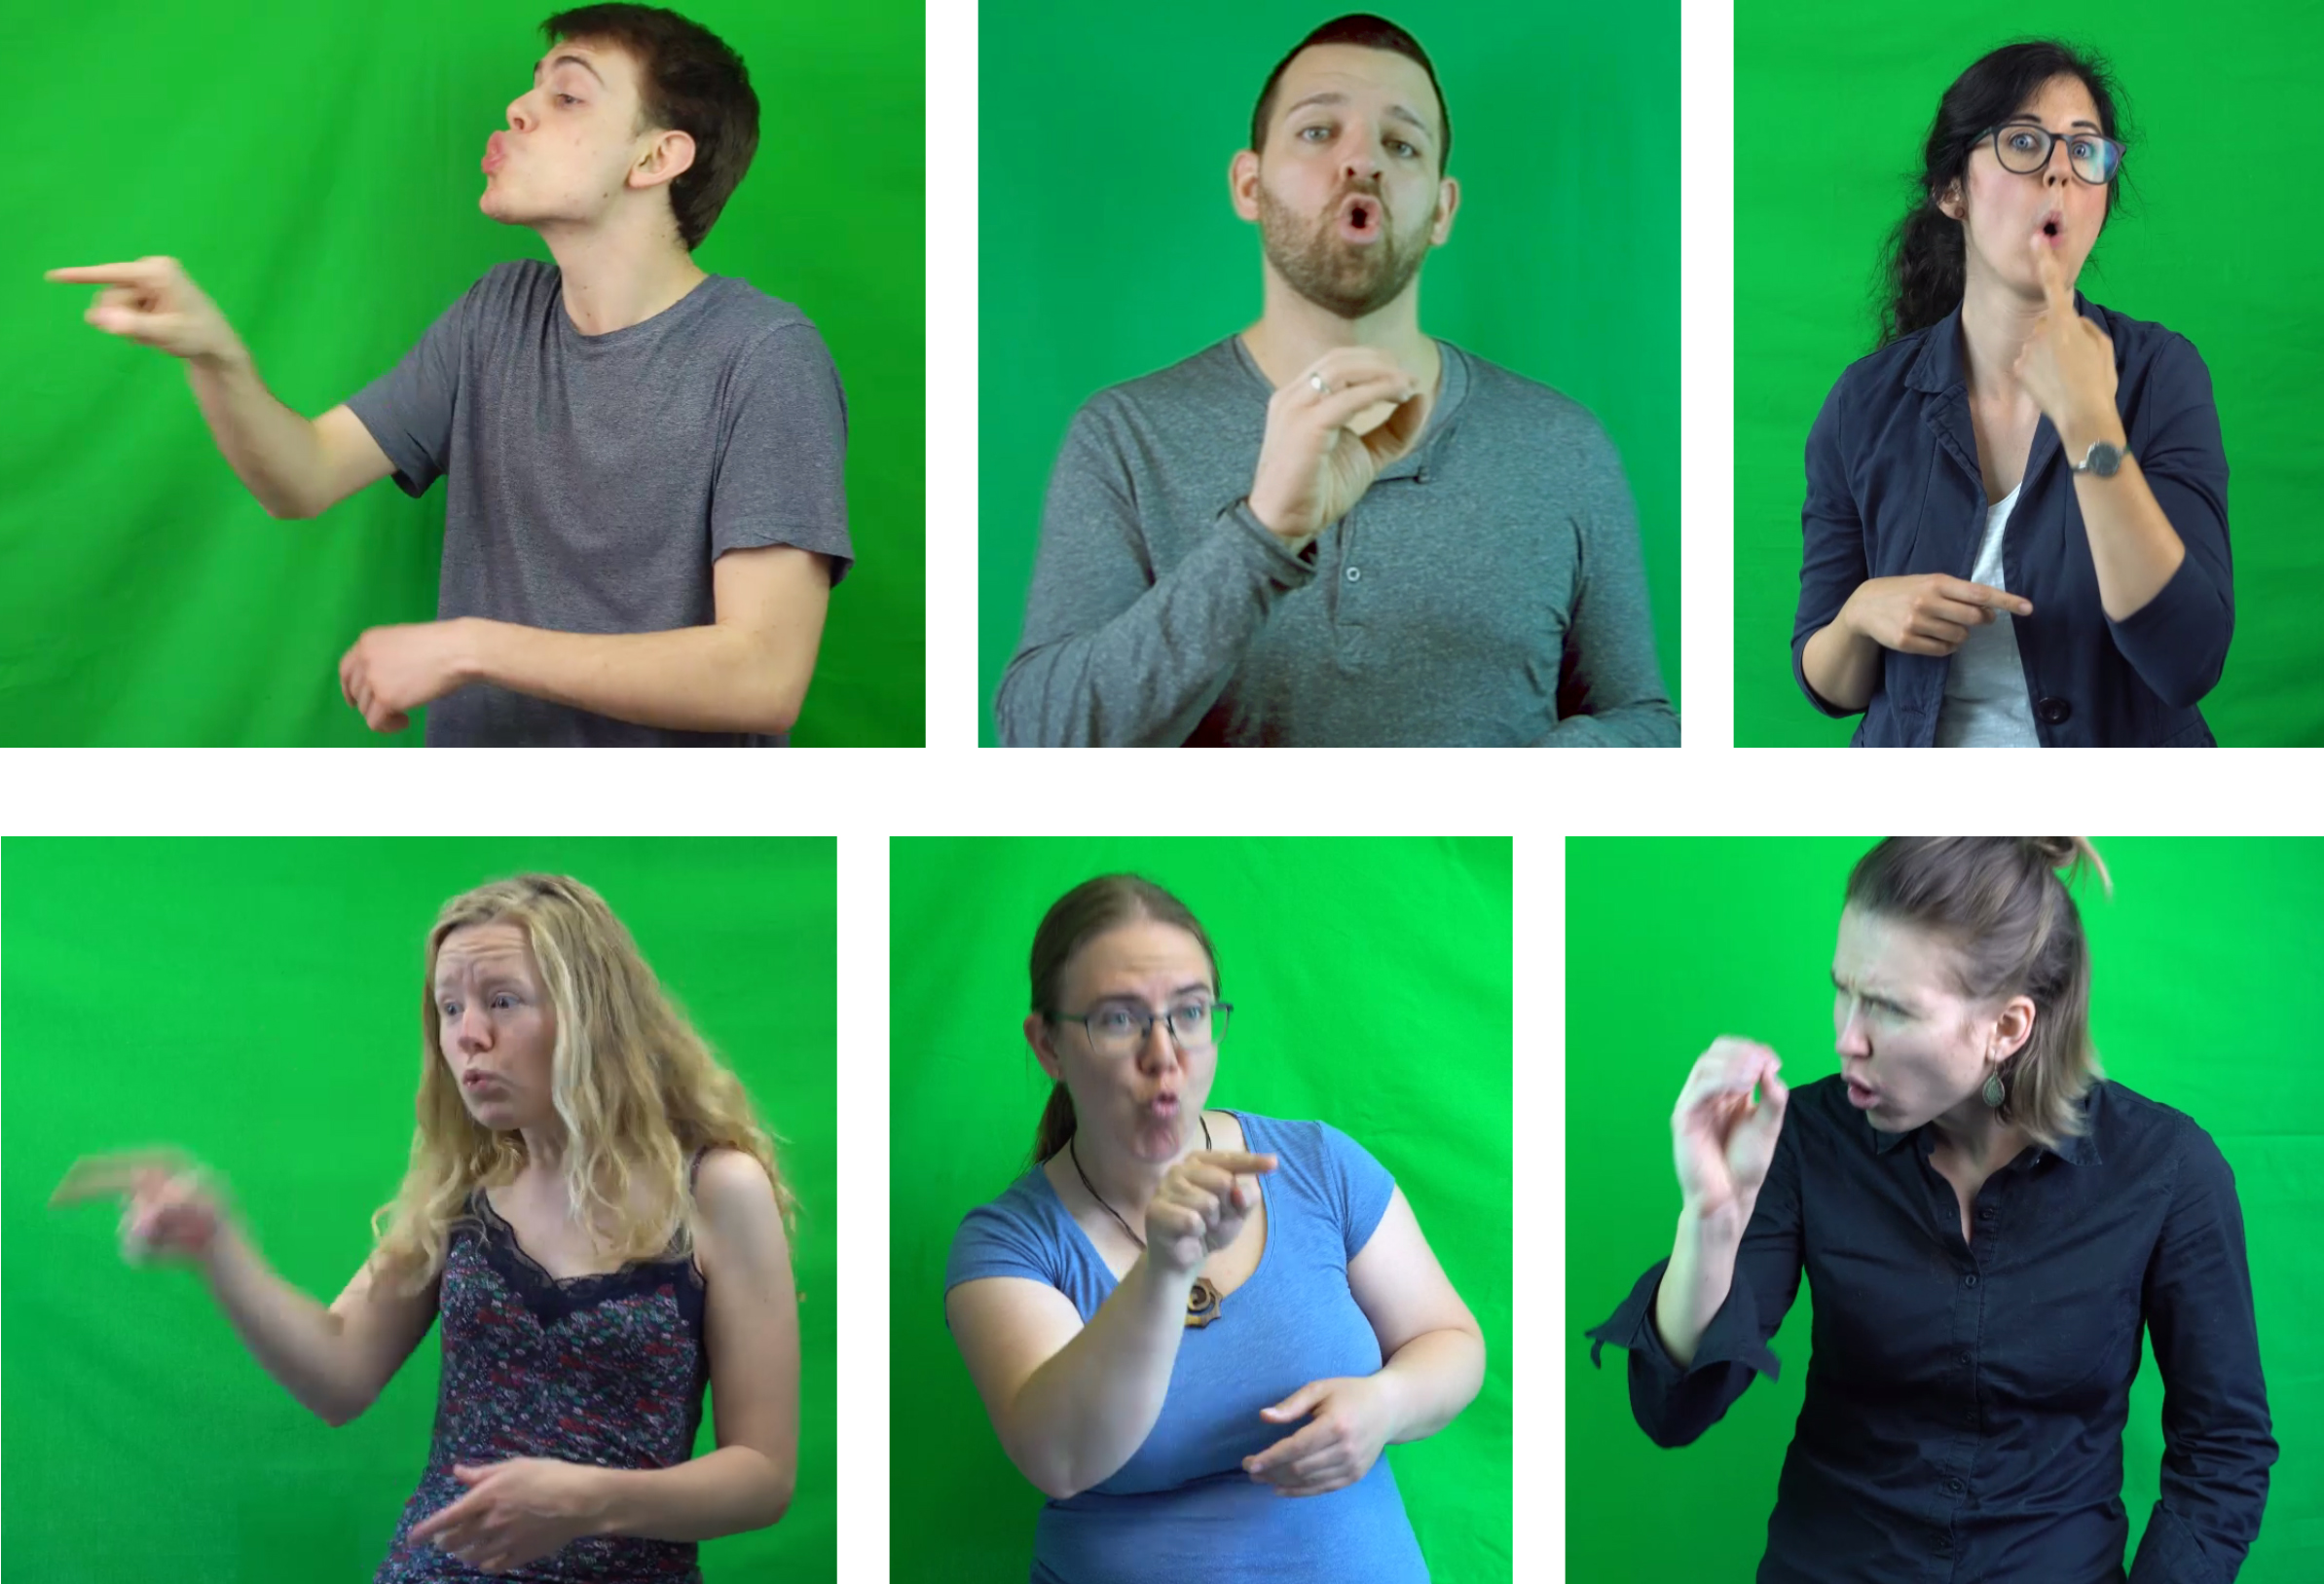
\includegraphics[width=1.0\textwidth]{contrastivefocus2.jpg}
	\caption{The non-manuals used with contrastive focus. Signers in the top row of the figure are from Baden-Württemberg, signers in the bottom row are from Bavaria.}
	\label{contrastivefocus}
\end{figure}

Contrastive focus can stay \textit{in-situ} in DGS, but can also be moved into a clause-initial position. Glossed examples are shown in (\ref{ex:contrastivefocusa}). The contrastive focus non-manuals are glossed `contr'.

\begin{exe}
\ex\label{ex:contrastivefocusa}\begin{xlist}
\ex
A: Paul bought beer yesterday. \\
B: \slg{yesterday} \slg[contr]{otto} \slg{beer buy}
%
%{} {\hspace{85pt}contr} {}   \\
%{B: \textsc{yesterday}} {$\overline{\textrm{\textsc{\textsc{otto}}}}$ \textsc{beer buy}}  
\glt \textcolor{white}{B: }`It was Otto who bought the beer yesterday.' \label{ex:contrastivefocusaa}
\ex
A: Paul bought beer yesterday. \\
B: \slg[contr]{otto} \slg{yesterday beer buy}
%
%{\hspace{18pt}contr} {}   \\
%{B: $\overline{\textrm{\textsc{\textsc{otto}}}}$ {\textsc{yesterday beer buy}}}  
\glt \textcolor{white}{B: }`It was Otto who bought the beer yesterday.' \label{ex:contrastivefocusab}


\end{xlist}
\end{exe}

\noindent However, a another possibility is that doubling is not related to focus, at least not to contrastive focus. Instead, it seems plausible to me that it is used as an emphasis device, but I will not pursue this option any further (but see \citealt{wilbur2012informationstructure}). Future research will also have to check if there is a difference -- maybe in exhaustiveness -- between moved and \textit{in-situ} contrastive focus. If this is not the case, one could assume that movement in the \textit{in-situ} cases only takes place at LF.

Taken together, contrastive focus is marked non-manually with the whole head and, in line with the bodily mapping hypothesis, with the eyebrows, although there is geographical variation with contrastive focus marking.

\subsubsection{Shoulder positions for contrasts}
As has been\is{shoulder positions} reported for other sign languages, contrastive focus is sometimes additionally marked by using the shoulders and locations in signing space. When two referents are contrasted, one is signed on one side on the body and the item to be contrasted on the other side. This is exemplarily shown in Figure (\ref{contrastiveshoulders}).


\begin{figure}[bt]
\centering
	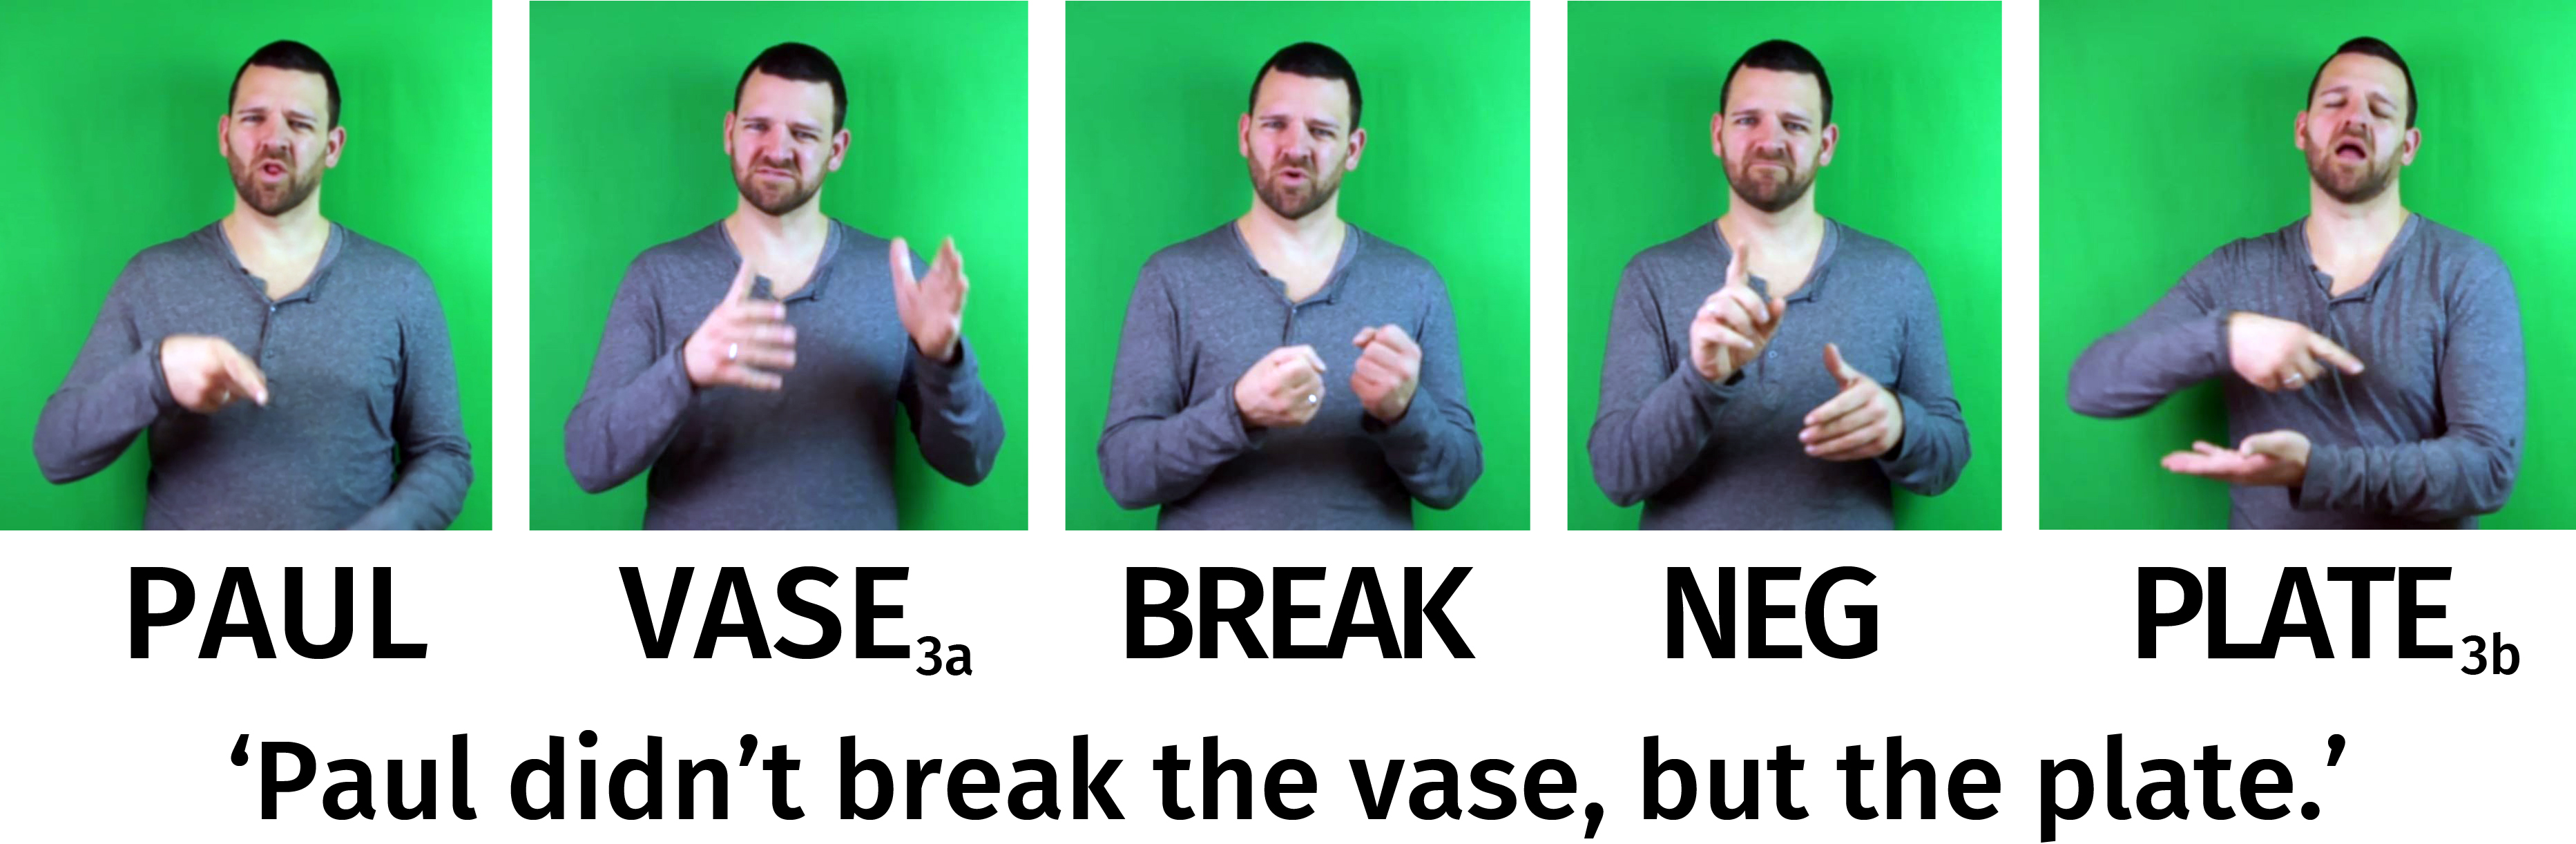
\includegraphics[width=1.0\textwidth]{contrastiveshoulders.jpg}
	\caption{An example of the use of signing space for contrasts.}
	\label{contrastiveshoulders}
\end{figure}

The example in the figure shows a sentence in which a vase is contrasted with a plate. While the signer locates the vase to his left in the example, the plate is located to his right. This is also mirrored by shoulder movement. This kind of opposition, however, is found in many other constructions, including plain coordination. 



Taken together, the structure of the focus phrase could be modeled in the way shown in (\ref{ex:focusphrasedgs}) if one allows heads to be right-branching. The other option would be to assume a left-headed focus phrase and additional XP movement into a higher specifier position.

\begin{exe}
\ex\label{ex:focusphrasedgs} 
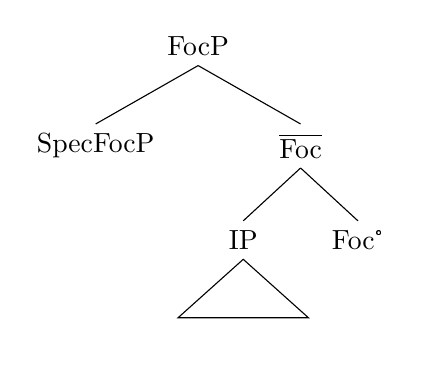
\begin{tikzpicture}[baseline=(current bounding box.north), scale=1.00]
\tikzset{level distance=35pt,sibling distance=5pt,every tree node/.style={align=center,anchor=north}}

\Tree [.FocP [.SpecFocP ] [.{$\overline{\textrm{Foc}}$} [.IP \edge[roof]; \node(t){\qquad \qquad}; ] [.{Foc\textdegree } ] ] ]
\end{tikzpicture}
\end{exe}

\noindent The landing site for contrastive focused material in the model in (\ref{ex:focusphrasedgs}) would then be SpecFocP and the landing site for focus doubles would be Foc\textdegree . Evidence for this structure comes from the fact that it is possible to combine contrastive focus and focus doubling within the same clause, as shown in (\ref{ex:contrastivefocusaabbb}).

\begin{exe}
\ex
A: Did Paul buy the beer yesterday? \\
B: \slg[contr]{index\textsubscript{2}} \slg{should beer buy} \slg[foc]{should}
%{} {\hspace{27pt}contr} {} {\hspace{128pt}foc}   \\
%{B:} {$\overline{\textrm{\textsc{index}\textsubscript{2}}}$} {\textsc{should beer buy} {$\overline{\textrm{\textsc{should}}}$}}  
\glt \textcolor{white}{B: }`It was \textsc{you} who \textsc{should} have bought the beer!' \label{ex:contrastivefocusaabbb}
\end{exe}

\noindent Future research could determine if and how it is possible to combine the different topics and contrastive focus with carefully constructed contexts. My preliminary impression from interviewing my consultants, however, is that it is -- similar to English -- not possible or at least very unnatural to combine one of the two topic expressions with contrastive focus in one clause.  



\is{focus|)}

\section{Sentence types, sentence mood, and illocutionary force}\label{sec:speechacts}
\is{sentence mood|(}\is{speech act|(}\is{illocutionary force|(}\is{sentence type|(}\is{mood|see{sentence mood}}\is{sentence mood}
The goal of the sections to follow is to discuss the encoding of speech acts (other than topics) in DGS. Before starting the discussion, some terminological remarks are in order since there is a plethora of related, but still different notions used in the literature. The notions that need clarification are `sentence type' (or `clause type'), `sentence mood', `illocutionary force', and `speech act'. I will follow a tradition that mainly comes from the German linguistics literature (e.\,g., \citealt{meibauer1987probleme, zaefferer1987satztypen, grewendorf1991theorien, brandt1992satztyp, zaefferer2006types, gutzmann2015use}). The differences between sentence types, sentence moods, and speech acts is one of linguistic perspective and goes back to the seminal observation of the division of labor between the semantic content of a sentence and the way the sentence is used by Gottlob Frege \citet[62]{frege1918gedanke}:\footnote{ English translation from \citet[329]{frege1997thought}. The original quote reads: ``Fragesatz und Behauptungssatz enthalten denselben Gedanken; aber der Behauptungssatz enthält noch etwas mehr, nämlich eben die Behauptung. Auch der Fragesatz enthält etwas mehr, nämlich eine Aufforderung. In einem Behauptungssatz ist also zweierlei zu unterscheiden: der Inhalt, den er mit der entsprechenden Satzfrage gemein, hat und die Behauptung.''}

\begin{quote}
An interrogative sentence and an assertoric one contain the same thought, but the assertoric sentence contains something else as well, namely assertion. The interrogative sentence contains something more too, namely, a request. Therefore two things must be distinguished in an assertoric sentence: the content, which it has in common with the corresponding propositional question; and assertion.
\end{quote}

\noindent Frege's idea was that the semantic content, i.\,e., the proposition of an assertion, a question, and an order could be one and the same and thus, there must be something else in a sentence that leads to the different meanings of these three types. For an illustration, consider the minimal pairs in (\ref{fregeillustrationa}), (\ref{fregeillustrationb}), and (\ref{fregeillustrationc}). All three sentence are about a person named Dede, a beer, and a drinking relation between Dede and the beer. Thus, they all have the same propositional content, or, as it was called in later works, they have the same `sentence radical' (\citealt[\S 22]{wittgenstein1953phil}; \citealt{stenius1967mood}). They only differ in what is called `sentence mood'. Thus, a sentence is always made up of two semantic parts, a sentence radical and a sentence mood. Sentence mood is sometimes written as an operator, as illustrated to the right of each sentence.


\begin{exe}
\ex\label{fregeillu}\begin{xlist} 
\ex Dede drinks a beer. \hfill {\textcolor{white}{!?}$\vdash$$[$\textsc{drink}(\textsc{Dede}, \textsc{beer})$]$} \label{fregeillustrationa}
\ex Is Dede drinking a beer? \hfill {\textcolor{white}{!$\vdash$}?$[$\textsc{drink}(\textsc{Dede}, \textsc{beer})$]$} \label{fregeillustrationb}
\ex Drink a beer, Dede! \hfill {\textcolor{white}{$\vdash$?}!$[$\textsc{drink}(\textsc{Dede}, \textsc{beer})$]$} \label{fregeillustrationc}
\end{xlist}
\end{exe} 

\noindent As the symbolic notations show, sentence mood operates over the whole sentence radical in each case. `Sentence mood' is a semantic term, as should have become clear from the discussion so far. The same phenomenon, i.\,e., the differences between the sentences in (\ref{fregeillu}), can also be viewed from syntax as each sentence has a different syntactic structure. This means, that each sentence has a specific morpho-syntactic form that is systematically linked to a specific type of meaning. This form of a sentence is called its `sentence type'. 

As sentence types (sometimes called `form types)' are syntactically defined they are described in syntactic terms (this can be done on different levels of precision). The example in (\ref{fregeillustrationa}), for example, can be called a verb second indicative sentence. Cross-linguistically, different syntactic structures (at least surface structures) are linked to the same meaning, i.\,e., the same sentence mood. I therefore choose a very coarse and simple terminology for sentence types: I will simply add the label `sentence' to the name of the mood. A sentence expressing declarative mood is thus called a `declarative sentence' or a sentence expressing interrogative mood, an `interrogative sentence'.

Although there is a relation between sentence type and sentence mood, there is no one-to-one mapping between them. There are, for example, different imperative sentence types, linked to imperative mood in German, as illustrated in (\ref{differntdorm}).


\begin{exe}
\ex German \label{differntdorm}\begin{xlist} 
\ex \gll {\textit{Trink}} {\textit{jetzt}} {\textit{sofort}} {\textit{ein}} {\textit{Bier}!}  \\
{drink} {now} {instantly} {a} {beer} \\
\trans `Drink a beer right now!' \label{differentformtypesa}
%\ex \gll {Du} {sollst} {jetzt} {sofort} {ein} {Bier} {trinken!}  \\
%{you} {should} {now} {instantly} {a} {beer} {drinking} \\
%\trans `You shall drink a beer right now!' \label{differentformtypesb}
\ex \gll {\textit{Dass}} {\textit{du}} {\textit{jetzt}} {\textit{sofort}} {\textit{ein}} {\textit{Bier}} {\textit{trinkst}!}\\
{that} {you} {now} {a} {beer} {drink} \\
\trans `Drink a beer right now!' \label{differentformtypesc}
\end{xlist}
\end{exe} 

\noindent The examples show that there are different ways to express an imperative in German. The example in (\ref{differentformtypesa}) shows a verb-first imperative sentence and (\ref{differentformtypesc}) a verb-last imperative sentence. Although they cannot be used interchangably, both sentence types encode imperative mood.

The term `sentence' is used here in a rather abstract way. Sentences do not exist in a vacuum, but are used, i.\,e., they are uttered. One and the same sentence can be used to achieve different goals. We can, for example, use a declarative sentence, such as \textit{Dede drinks a beer} (\ref{fregeillustrationa}) to make an assertion. However, the same sentence could be used as an order, for example, when uttered to a bartender. Therefore, there is no one-to-one mapping, but rather a mapping between sentence type and the speech-acts that can be performed with them. From this, we can derive 

\begin{quote}
$[$\dots $]$ that it is only the communicative potential of a sentence, a default interpretation, that is determined by its formal and semantic properties. The precise speech act performed by an utterance is the result of an interaction between these properties and various contextual factors, such as the social situation, the current state of an interaction and the background knowledge of speaker and hearer. \citep[277]{konig2007speech}
\end{quote} 

\noindent A `speech act' is defined as the performative function a sentence fulfills when uttered \citep{austin1962things}. To be more precise, a speech act is an action that is used by a speaker or signer to achieve a certain goal. Such goals can be to add information to the current information storage shared by the interlocutors (i.\,e., to make an assertion), to ask an interlocutor to provide information that the signer/speaker is missing (i.\,e., to ask a question), to make the hearer do something (i.\,e., to make a directive), or to express surprise (i.\,e., to make an exclamation). A speech act consists of two parts: a proposition and a(n) (illocutionary) force. The latter is the aspect of meaning that makes clear whether the utterance should be understood as an assertion, a question, a directive, a warning etc. While there may be no one-to-one mapping between sentence mood and illocutionary force, sentence mood nevertheless has a prototypical illocutionary force associated with it. This is plausible because, under normal circumstances, a hearer infers the force of an utterance from a combination of three sources:\label{threesources} the context, the mood (encoded by a certain sentence type), and the proposition expressed. Without contextual enrichment, a declarative is understood as a statement, an interrogative as a question, and an imperative as an order, or more broadly speaking as a directive. Thus, when no context is present, the mood (i.\,e., the semantics) leads to a prototypical reading.


Typologically, it is assumed that all languages exhibit declarative, interrogative, and imperative sentences as basic sentence types (e.\,g., \citealt{lyons1977semantics, sadock1985speech}). This means that it is not only taken as a universal that statements, questions, and orders can be expressed in all languages, but that all languages have syntactic means to encode those communicative functions. Table \ref{basicsentencetypes} shows the three basic sentence types, the sentence moods they are prototypically linked to, and the speech acts that they are primarily used for. Somewhat surprisingly, it is only these three sentence types that are universal, and no language was found to grammaticalize, e.\,g., the expression of warnings, promises, or acts of forgiveness. Nevertheless, there are languages that have means to express sentence types other than declaratives, interrogatives, and imperatives, for example, exclamatives (for the expression of exclamations), optatives (for the expression of desires), or exhortatives (incentives for joint action).

\begin{table}[t]
\centering

\begin{tabular}{p{4cm}p{3.2cm}p{4cm}}
\lsptoprule
\textsc{Sentence type} & \textsc{Sentence mood} & \textsc{Illocutionary force} \\
\midrule
\rowcolor[gray]{.9}
Declarative sentence & Declarative & Assertion \\
Interrogative sentence & Interrogative & Question \\
\rowcolor[gray]{.9}
Imperative sentence & Imperative & Directive \\
%\rowcolor[gray]{.9}
%Exclamative sentence & Exclamative & Exclamation \\
\lspbottomrule
\end{tabular}
\caption{Basic sentence types}
\label{basicsentencetypes}
\end{table}

That all languages exhibit encoding strategies for declarative, interrogative, and imperative clauses and that some even use grammatical heads with phonological content for their encoding, lead several authors to the conclusion that there exist dedicated functional projections to encode their respective illocutionary force (e.\,g., \citealt{rizzi1997fine, cinque1999adverbs, ambar2003}). This does not mean that every possible speech act has its own phrase, but it is usually assumed that there only exists such a phrase for the three basic sentence types, as they are (more or less) directly linked to an illocutionary force (e.\,g., \citealt{speas2003configurational}).

In the following sections I will discuss declaratives, interrogatives, imperatives, and make some brief remarks on optatives. In each section, I will (i) first briefly give a cross-linguistic overview of the sentence type under discussion, often accompanied by exemplary analyses from the literature, (ii) review how the respective sentence type is expressed in other sign languages, again accompanied by exemplary analyses from the literature, and finally (iii) discuss and analyze the sentence type in German Sign Language.

\is{sentence mood|(}\is{speech act|)}\is{illocutionary force|)}\is{sentence type|)}
%\clearpage

\section{Declarative sentences}\label{declarativesentences}
The discussion of declarative sentences is, compared to other sentence types, usually rather short. I will follow this tradition in this section. As with the following sections, I will first give a short overview of the situation found in spoken languages, followed by a brief description of what is known about the phenomenon under discussion in sign languages and will then describe the situation for DGS. 


\subsection{General overview}
%\subsubsection{Declaratives and Intonation}
As the present and the following chapter include the discussion of non-manual markings, and as non-manual markings in sign languages are often equated with intonation in spoken languages, I will start the discussion of declaratives in spoken languages with intonation and then proceed with a brief remark on declaratives and word order.

Many spoken languages make use of intonational means to distinguish between different sentence types. Although declaratives represent the unmarked case, they are not simply marked by a flat intonational contour in many languages. Instead, spoken languages often seem to pursue the strategy of making declaratives and interrogatives as distinct as possible. In English, for example, declaratives are prototypically associated with a falling, and interrogatives with a rising intonation (e.\,g., \citealt{gunlogson2002declarative}). This is, however, far from being a universal, as in many languages, for example in Romanian or Hungarian, both declarative and (polar) interrogative sentences receive a raising-falling intonational pattern that is very similar in both sentence types (e.\,g., \citealt{ladd1981intonational}).


In the following, I will describe what is known about declarative sentences in sign languages. First, I will briefly discuss non-manual markings, the counter-part of spoken language intonation, and then give a short overview of the constituent order typology. 

\subsection{Declaratives in sign languages}
\subsubsection{Non-manual markings}
Descriptions of declaratives are, as already noted at the beginning of the section, rather short, despite being the most common and unmarked sentence type. \citet[289]{signgram2017}, in the SignGram Blueprint, for example, report:

\begin{quote}
Sign languages make use of declaratives just like spoken languages. However, the grammar writer will not easily find studies, journal papers, articles, or book chapters devoted to declaratives.
\end{quote}

\noindent While declaratives in many spoken languages do not usually exhibit a flat intonational contour, non-manual markings spreading over the whole clause as found in other sentence types, such as interrogative or imperative sentences, are absent in declaratives -- disregarding cases of evaluation, epistemicity, or evidentiality that will be discussed in the next chapter.

\subsubsection{Declaratives and the basic constituent order in sign languages}
Declaratives are important to determine the basic word order of a language (often alternatively called `constituent order' in the sign language linguistics tradition). A basic declarative sentence in American Sign Language, for example, takes the form illustrated in (\ref{aslbasicwordorder}), from \citet[81]{neidle2000syntax}. 

\begin{exe}
\ex American Sign Language\\
\textsc{john like chocolate} 
\glt `John likes chocolate.'\label{aslbasicwordorder}
\end{exe} 

\noindent From unmarked examples like the on in (\ref{aslbasicwordorder}), it was inferred that the basic word order of American Sign Language is SVO \citep{fischer1975influences}. Typologically, the word order generalizations from research on spoken languages fit well into what is known about sign languages. Based on a sample of 42 sign languages, \citet{napoli2014order} report that all studied languages either exhibit an SOV or SVO order, with SOV being a grammatical order in all sign languages included in the study. For similar conclusions see \citet{kimmelman2012word}.

As in spoken languages, deviations of the basic word orders are described for sign languages. This is, for example, the case with topicalizations and other fore- or backgrounding processes. Besides topicalizations or for focusing purposes, some other factors leading to word order changes, which are not necessarily familiar based on research on spoken languages, were described for sign languages. These include the agreement properties of the verb and word order changes in locative sentences. I will briefly discuss both phenomena in the following section, as both are found in German Sign Language.

\subsection{Declaratives in DGS}
\subsubsection{Non-manual markers in DGS declaratives}

Declaratives in DGS are produced without any additional non-manual markings, i.\,e., the facial expression is neutral, as long as the sentence does not contain any manual signs that are specified for a non-manual, there is no element receiving stress, and no additional layer of information (such as evaluation, epistemicity or role-shift indicating that the information conveyed is reported from a perspective different from the signer's \textit{hic-nunc-ego origo}; \citealt{buhler1934}) is present. In this respect, DGS behaves just like other sign languages. 

\subsubsection{Some notes on DGS constituent order}\is{word order|see{constituent order}}\is{constituent order}
As already noted (see Section \ref{basicclausstructuredgs}), the unmarked word order of German Sign Language is SOV -- in matrix and in embedded clauses (\citealt{keller1998aspekte, steinbach2013satztypen}. This is illustrated in (\ref{dgsunmarkedwordorder}).

\begin{exe}
\ex \textsc{Marjolaine beer buy}
\glt `Marjolaine bought a beer.'\label{dgsunmarkedwordorder}
\end{exe}

\noindent An OV analysis is supported by the fact that determiners and adpositions are found after their complements, and that modals and negation (when expressed manually) follow rather than precede the verb \citep{pfauquer2007syntaxofnegationandmodals,bross2017scope}.


Topicalizations as well as other fore- and backgrounding processes can alter the basic SOV order. While such pragmatic highlighting is usually visible as it is marked non-manually and/or prosodically, there are some cases in which an SVO order is possible without any additional marking. Thus, SOV structures like the one in (\ref{sovsvodgsa}) and SVO structures like in (\ref{sovsvodgsb}) can be used equally. In most cases this concerns volitional verbs like \textsc{like} which I will discuss in Section \ref{volition}.\is{volition}

\begin{exe}
\ex\label{sovsvodgsa}
\textsc{Marjolaine beer like}
\glt `Marjolaine likes beer.'\label{sovsvodgsaaba}
\end{exe}

\begin{exe}
\ex\label{sovsvodgsb}
\textsc{Marjolaine like beer}
\glt `Marjolaine likes beer.'
\end{exe}


\noindent Although SVO orders like in (\ref{sovsvodgsb}) are sometimes found, SOV orders represent the clear majority. Thus, SOV can be taken as the most unmarked constituent order in DGS.% -- nevertheless, future research should take a deeper look into the OV/VO alternation and try to find out which discourse conditions lead to the SVO structures or if there are any changes in meaning associated with the two structures. 

Additionally, the word order in locative sentences usually deviates from the SOV order. As in many other sign languages, locative sentences exhibit an OSV word order in DGS, as illustrated in (\ref{locativesentence}). An alternative analysis would be that sentences of this type in fact do not deviate from the SOV constituent order and instead include two predications as indicated by the second paraphrase. 

\begin{exe}
\ex \textsc{pond index}\textsubscript{3a} \textsc{fish swim}\textsubscript{3a}
\glt `Fish were swimming in the pond./There was a pond. Fish were swimming in it.' \label{locativesentence}
\end{exe}

\noindent For locative\is{locative sentences} sentences as in (\ref{locativesentence}), it is usually argued that the driving force behind their constituent order derives from a figure-ground principle which states that grounds (bigger and more immobile referents) are introduced before figures (smaller and more mobile) referents \citep{volterra1984italian,kimmelman2012word,pfau2016simple}. Some authors (e.\,g., \citealt{perniss2007space, ozyurek2010locative}) argue that the driving force behind the word order in locative sentences is iconicity. It seems plausible that this kind of word order variation is driven by pragmatic factors. It seems to be a general rule of a conversation to first introduce the ground. It would be rather unnatural to utter a sentence like \textit{Fish were swimming in the pond} without the speaker first mentioning that there was a pond or, at least, that s/he was in a garden. While English has a very strict word order, many other languages, including Italian and German, have more freedom in either mentioning the ground or the figure first in locative sentences, as shown for German in (\ref{germanlocative}).

\begin{exe}
\ex German \label{germanlocative}\begin{xlist} 
\ex \gll {\textit{Im}} {\textit{Teich}} {\textit{schwammen}} {\textit{Fische}}\\
{In.the} {pond} {swam} {fish}  \\
\trans `Fish were swimming in the pond.' \label{germanlocativea}
\ex \gll {\textit{Fische}} {\textit{schwammen}} {\textit{im}} {\textit{Teich}}  \\
{Fish} {swam} {in.the} {pond} \\
\trans `Fish were swimming in the pond.' \label{germanlocativeb}

\end{xlist}
\end{exe} 

\noindent Although this claim needs empirical validation by future studies, it seems that sentences with a figure-ground order as in (\ref{germanlocativea}) are more suitable in situations in which the ground was not mentioned before and the order ground-figure as in  (\ref{germanlocativeb}) are more natural in situations in which the ground was already introduced in the discourse. My DGS data also points in this direction. While the consultants clearly preferred the ground-figure order (i.\,e., OSV structures), they also allowed the reverse pattern (i.\,e., SOV structures) in locative contexts, as shown in  Figure \ref{fig:figuregroundcat}.

\begin{figure}[bt]
\centering
	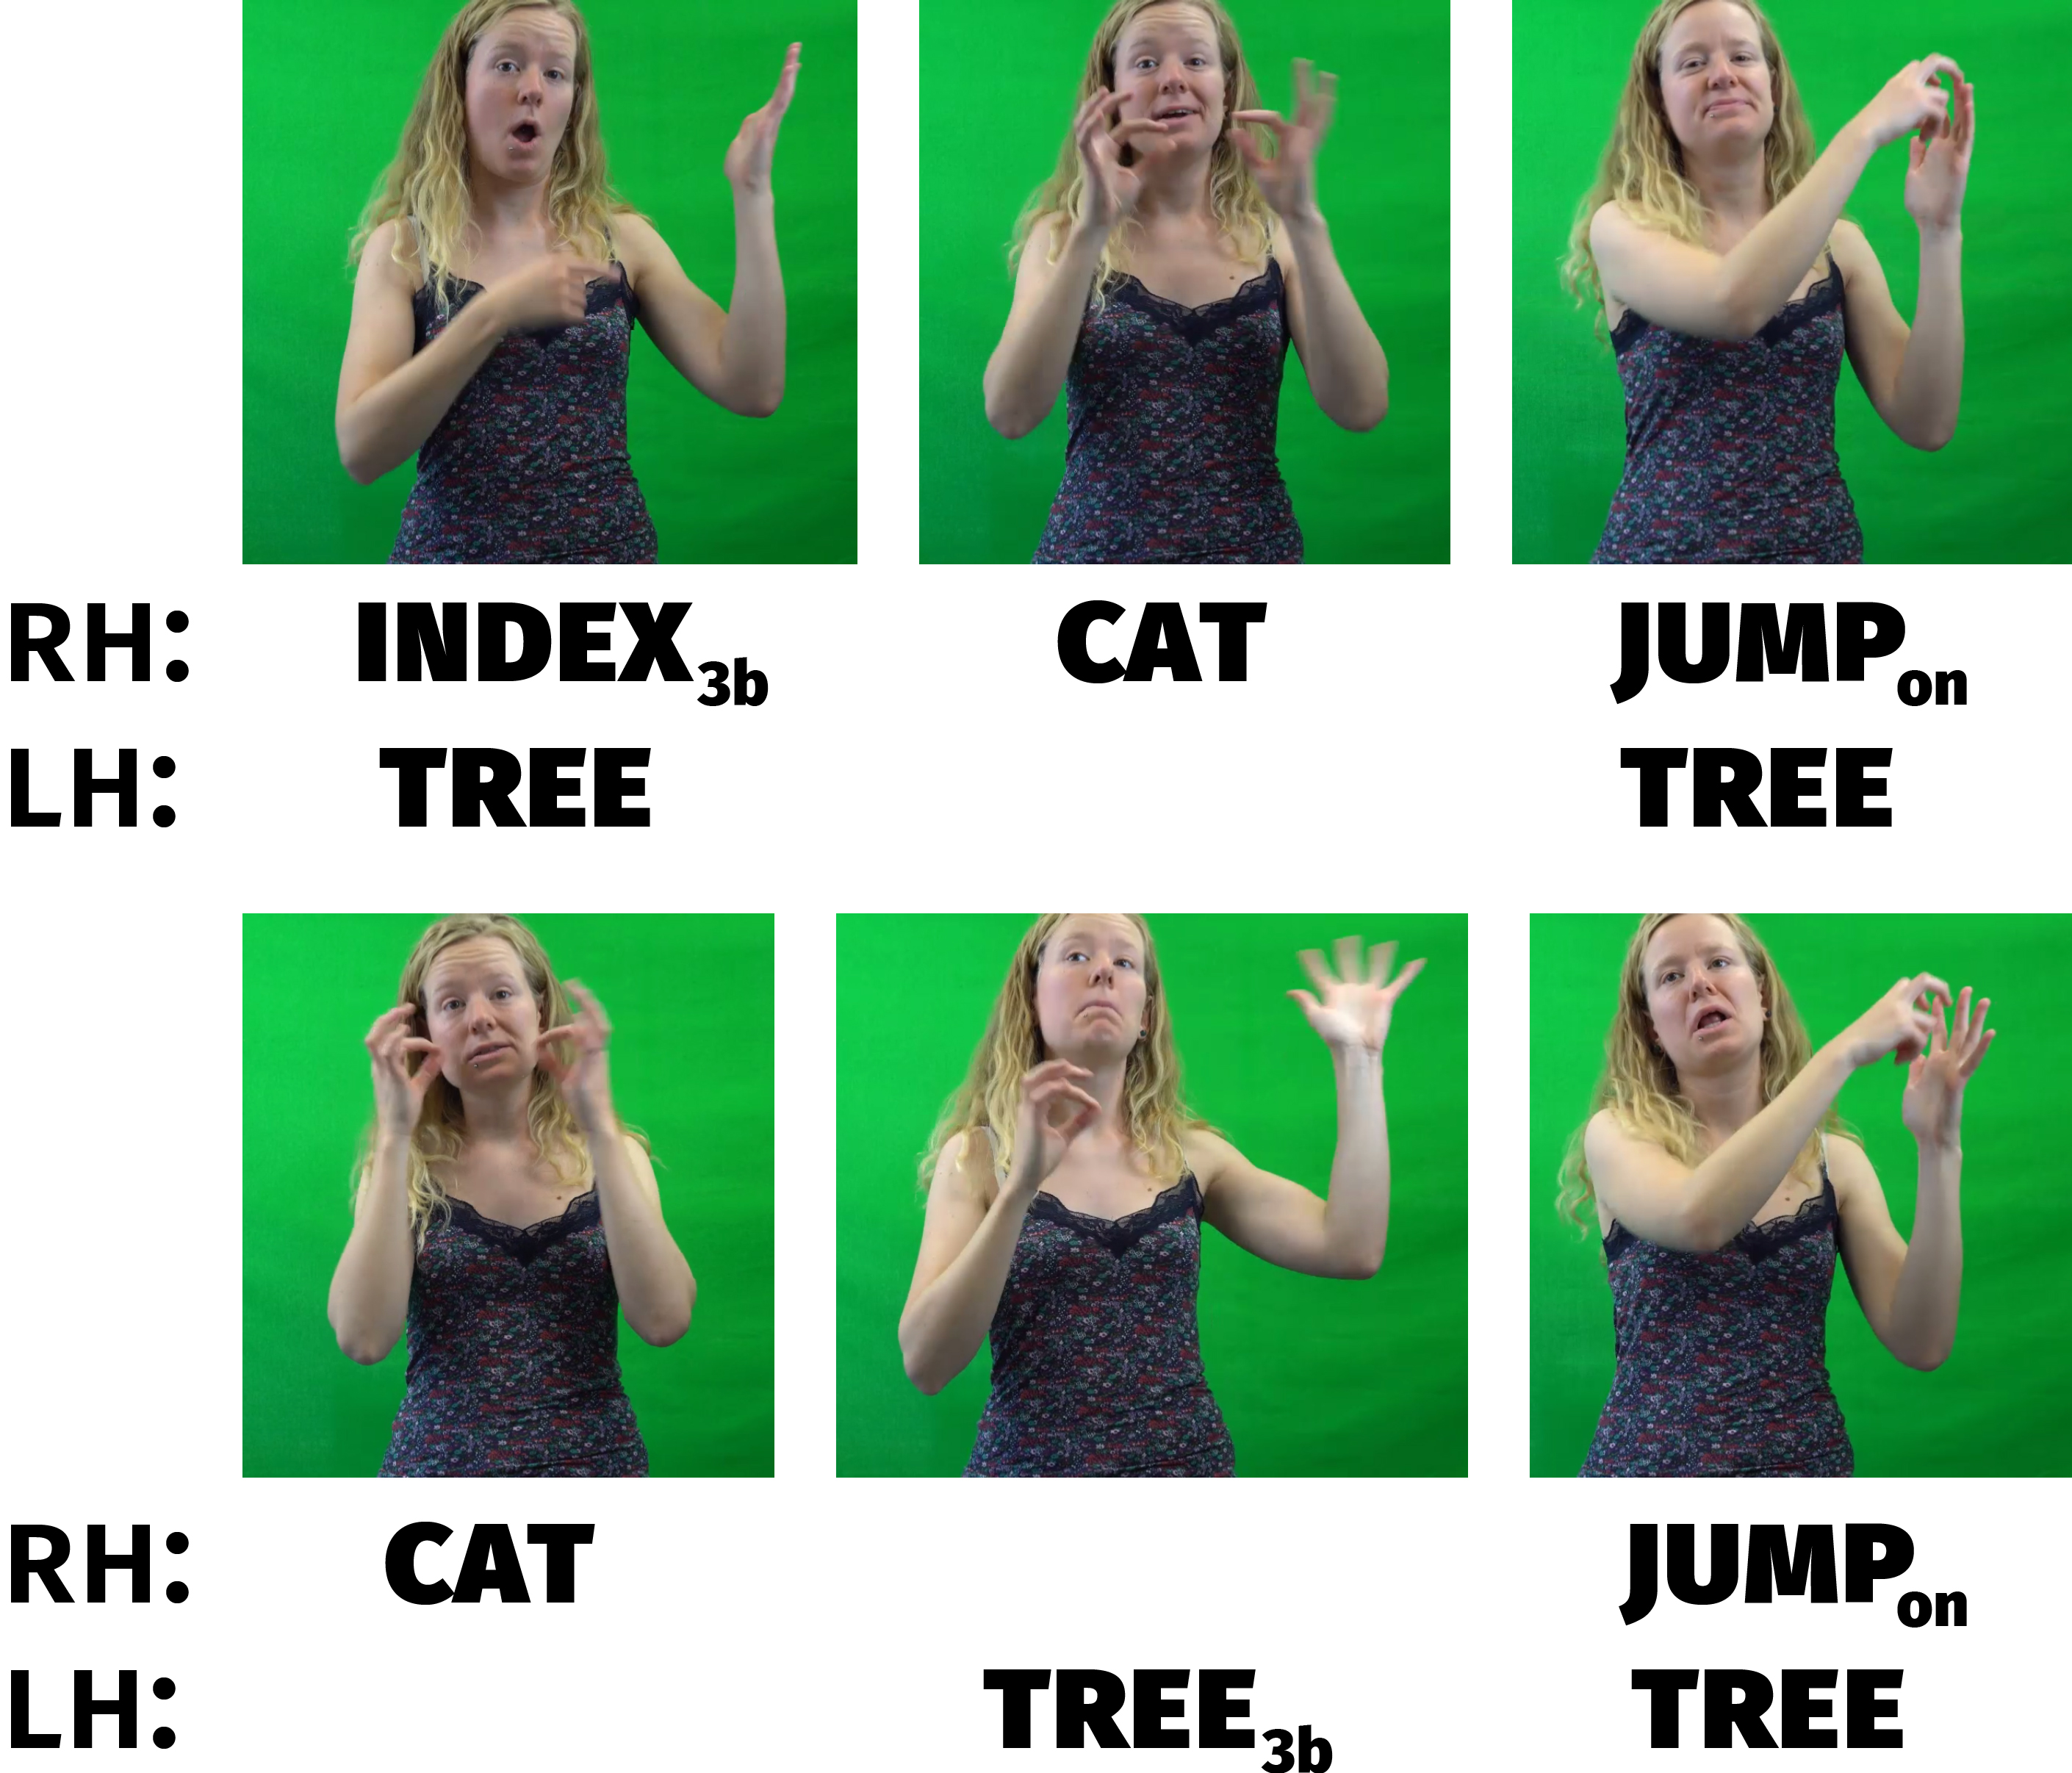
\includegraphics[width=1.0\textwidth]{figuregroundcat.jpg}
	\caption{There are two options for expressing locative sentences in DGS. The top example shows a sentence in which the ground was not introduced in the previous discourse. In the bottom example, the ground was already introduced. The abbreviations `LH' and `RH' stand for left hand and right hand respectively.}
	\label{fig:figuregroundcat}
\end{figure}

What is interesting about the sentences in Figure \ref{fig:figuregroundcat} is that the ground is introduced by an index sign in the ground-figure sentence (top example) while this index is missing in the SOV sentence on the bottom of the figure. One could either argue that the ground is introduced first (as in spoken languages) in examples of the first kind leading to a deviation in constituent order or that the order in examples of the first kind, in fact, does not deviate, but that sentences of this kind consist of two clauses: the first one being an existential clause (`There is a tree') and the second one being the locative sentence (`The cat jumped on it'). 

Taken together, the vast majority of declarative sentences in DGS that are not highlighted in some way follow a more or less strict SOV pattern. Next, I will discuss polar interrogative sentences. Again, I will briefly outline the situation for spoken languages (Section \ref{generalpolar}), followed by a discussion of polar questions in sign languages (Section \ref{polarintsign}), and finally, sketch and analyze the phenomenon in DGS (Section \ref{polarinterrogativesdgs}).

\section{Polar interrogative sentences}\label{polargeneralsectionlabel}
\is{yes/no questions|see{polar interrogatives}}
\is{polar interrogatives|(}
This section is concerned with polar interrogatives. Again, I will briefly describe the situation in spoken languages (Section \ref{generalpolar}), the situation in sign languages (Section \ref{polarintsign}), and then discuss and analyze the phenomenon in DGS (Section \ref{polarinterrogativesdgs}). From the spreading behavior of the non-manuals used in polar interrogatives in DGS and distributional facts of manual signs that are probably related to FocP and IntP, I will discuss two modeling possibilities: either the  CP projection encoding interrogative force is right-headed or, alternatively, the projection is left-branching and the lexical material in polar interrogatives moves to this projection for feature-checking purposes. % the higher CP area encoding interrogative force are right-headed.


\subsection{General overview}\label{generalpolar}

\subsubsection{General introduction}
Polar interrogatives are sentences that are typically used to ask yes/no questions, i.\,e., questions that can be answered with `yes' or `no'. Cross-linguistically, there is much variation concerning the marking involved in polar interrogatives. Many, but not all languages use a special intonational contour (mainly rising final intonation), an initial or final question particle, special verb morphology, or a change in word order (\citealt[181--182]{sadock1985speech}; \citealt{dryer2013questions}). 

In the following, I will exemplarily discuss two strategies for expressing interrogative sentences in spoken languages and how they were analyzed. First, I will outline polar question formation in English and then discuss the same sentence type in the Gungbe language Gbe. Although the strategies used in both languages are superficially very dissimilar, both languages were analyzed as involving an interrogative feature in the left periphery.

\subsubsection{Polar interrogatives in English}

In English, we find intonational marking as well as a change in word order. To be more precise, we find a rising intonation and subject-auxiliary inversion. This is shown in (\ref{simpleenglishpolarinterr}).

\begin{exe}
\ex\label{simpleenglishpolarinterr}\begin{xlist}
\ex Daniel will visit his neighbor. \hfill Declarative\label{simpleenglishpolarinterraaaa}
\ex Will Daniel visit his neighbor? \hfill Polar interrogative\label{simpleenglishpolarinterrbbbb}
\end{xlist}
\end{exe} 

\noindent English declaratives exhibit the order subject--auxiliary--verb, as illustrated in (\ref{simpleenglishpolarinterraaaa}). In polar interrogatives (\ref{simpleenglishpolarinterrbbbb}), the auxiliary \textit{will} raises into a higher position than the subject \textit{Daniel}. The same pattern is found in examples without auxiliaries. To do this, English makes use of \textit{do}-support, as illustrated in (\ref{simpleenglishpolarinterrtwo}).

\begin{exe}
\ex\label{simpleenglishpolarinterrtwo}\begin{xlist}
\ex Daniel visits his neighbor. \hfill Declarative\label{simpleenglishpolarinterra}
\ex Does Daniel visit his neighbor? \hfill Polar interrogative\label{simpleenglishpolarinterrb}
\end{xlist}
\end{exe} 

\noindent Standard analyses of English polar interrogatives assume that the purpose of the insertion (or the movement) of the auxiliary into a higher position is feature checking. \citet{roberts1993}, for example, assumes that the CP hosts a null question operator in English that triggers this kind of movement. Evidence for this comes, for example, from the fact that when an overt complementizer introducing a polar interrogative is present, as is the case in embedded questions, verb movement is blocked. This is illustrated in (\ref{englishembeddedquestions}).%Evidence for this comes %from different sources. I will just briefly sketch two of these sources.

\begin{exe}
\ex\label{englishembeddedquestions}\begin{xlist}
\ex \textcolor{white}{*}Bill asks whether Maria will come. \label{englishembeddedquestionsa}
\ex *Bill asks whether will Maria come.  \label{englishembeddedquestionsb}
\end{xlist}
\end{exe} 

\noindent Assuming that \textit{whether} is located in C\textdegree , we can assume that the auxiliary moves into exactly this position as it is not possible for the auxiliary to be hosted there when the position is taken by complementizers like \textit{whether} or \textit{if}.

The general assumption is that C\textdegree\ inherits a question feature or a question operator $[$Q$]$ that triggers subject-auxiliary inversion in root questions and that in embedded questions this feature is associated with a complementizer. For some researchers, most prominently \citet{cheng1997typology}, the movement of the auxiliary into C\textdegree\ is the crucial operation in clause-typing. 

\subsubsection{Polar interrogatives in Gbe}
In general, however, it should be stated that the processes underlying polar interrogatives are not well understood -- at least from a cross-linguistic perspective. This becomes obvious from the fact that there are many different mechanisms in the languages of the world that starkly differ from English (in fact, the subject-auxiliary inversion employed in English seems to be cross-linguistically a non-standard mechanism for marking polar questions, see \citealt{ultan1978some}). One such example are languages with clause-final question particles or languages with clause-final tonal question markers.

An example of the latter case is the Gbe language Gungbe\label{gungbepolar} spoken in Benin. In this language, the difference between a declarative and a polar interrogative is marked by a clause-final floating low tone as illustrated by the minimal pair from \citet[93]{aboh2010sa}.\footnote{ Tonal contours are indicated by accents. An acute (e.\,g. \textit{á}) represents a high tone, a grave (e.\,g. \textit{à}) a low tone, and a circumflex (e.\,g. \textit{\^{a}}) a high-low sequence.}

\begin{exe}
\ex Gunbe\label{yesnoquestiongungbe}
\begin{xlist}
\ex \gll {\textit{Sɛ́tɔ̀}} {\textit{kò}} {\textit{wá?}} \\
{Seto} {already} {come}\\
\trans `Seto arrived already.' \label{yesnoquestiongungbea} \hfill Declarative
\ex {\gll {\textit{Sɛ́tɔ̀}} {\textit{kò}} {\textit{w\^{a}?}} \\
{Seto} {already} {come.\textsc{inter}} \\
\trans `Has Seto arrived yet?' \label{yesnoquestiongungbeb} \hfill Polar question}
\end{xlist}
\end{exe}

\noindent The difference between a Gungbe declarative and a Gungbe polar interrogative is, as the examples illustrate, the floating low tone only present in polar interrogatives (in the example, on \textit{w\^{a}}). In embedded polar questions both the floating low tone and an interrogative complementizer (an equivalent of English \textit{whether}) are present, as shown in the minimal pair in (\ref{yesnoquestiongungbetwo}), again from \citet[93]{aboh2010sa}.

\begin{exe}
\ex Gungbe\label{yesnoquestiongungbetwo}\begin{xlist}
\ex {\gll {\textit{Ùn}} {\textit{sè}} {\textit{ɖɔ̀}  } {\textit{Sɛ́tɔ}̀} {\textit{kò}} {\textit{wá?}} \\
{1\textsc{sg}} {hear} {that} {Seto} {already} {come} \\
\trans `I heard that Seto has already arrived.' \label{yesnoquestiongungbetwoa} \hfill Embedded declarative}
\ex {\gll {\textit{Ùn}} {\textit{kànbíɔ̀}} {\textit{ní}} {\textit{Sɛ́tɔ}̀} {\textit{kò}} {\textit{w\^{a}?}} \\
{1\textsc{sg}} {ask} {if} {Seto} {already} {come.\textsc{inter}} \\
\trans `I asked if Seto has already arrived.' \label{yesnoquestiongungbetwob} \hfill Embedded polar question}
\end{xlist}
\end{exe}

\noindent Other Gbe languages exhibit clause-final question particles and other structurally high categories, such as encoding the speaker's point of view, are also realized as clause-final heads \citep[211--213]{lefebvre2006creole}. Following \citeauthor{kayne1994antisymmetry}'s (\citeyear{kayne1994antisymmetry}) idea that heads always precede their complements, \citet{aboh2004morphosyntax} and  \citet{aboh2004left} argue that the interrogative feature, labeled $[+$interrogative$]$ here, located in the head of a (left-headed) interrogative phrase (IntP) attracts the whole proposition in a Gungbe polar interrogative into its specifier. This is illustrated, in a slightly simplified version, in the tree in (\ref{ex:gungbepolarinterrogativetree}).

\begin{exe}
\ex\label{ex:gungbepolarinterrogativetree} 
\begin{adjustbox}{width=\linewidth}
\begin{tikzpicture}[baseline=(current bounding box.north), scale=0.80]
\tikzset{level distance=35pt,sibling distance=5pt,every tree node/.style={align=center,anchor=north}}
\Tree [.ForceP [.{SpecForceP} ] [.{$\overline{\textrm{Force}}$} [.{Force\textdegree } ] [.InterP [.SpecInterP \edge[roof]; \node(sleepyman){S\'{ɛ}t\`{ɔ} kò w\^{a}?}; ] [.{$\overline{\textrm{Inter}}$} [.{Inter\textdegree } {$[+$interrogative$]$} ] [.TopP [.SpecTopP ] [.{$\overline{\textrm{Top}}$} [.{Topic\textdegree } ] [.FocP [.SpecFocP ] [.{$\overline{\textrm{Foc}}$} [.{Foc\textdegree } ] [.IP \edge[roof]; \node(t){\qquad \textit{t} \qquad}; ] ] ] ] ] ] ] ] ]
\draw[semithick,->] (t)..controls +(south west:4) and +(south:2)..(sleepyman);

\end{tikzpicture}
\end{adjustbox}
\end{exe}


\noindent The tree shows a derivation of the simple polar question in (\ref{yesnoquestiongungbeb}) -- for a better orientation, I included the force, the topic and the focus projection. Evidence that such a phrasal movement analysis is plausible comes from topic and focus marking (and the fact that complementizers dominate embedded questions in the expected way (\ref{yesnoquestiongungbetwo}), where the complementizer would be located in the Force\textdegree\ in the tree). \citet{aboh2004left} shows that Gungbe has overt topic and focus markers which have to appear in a fixed order. Additionally, the topic and the focus markers appear in the expected clause-initial positions. An illustrative example of a topic and focus marker in an embedded clause is shown in (\ref{topicfocusmarkergungbe}).

\begin{exe}
\ex Gungbe \citep[168]{aboh2004left} \\ {\gll {\textit{Ùn}} {\textit{ɖɔ̀}} {\textit{ɖɔ̀}} {\textit{làn}} {\textit{l}ɔ̀} {yà} {\textit{Kòfí}} {\textit{wɛ́}} {\textit{Àsíbá}} {\textit{ní}} {\textit{ɖ}\textit{àɛ}} {\textit{n\'{a}}}  \\
{1\textsc{sg}} {say} {that} {meat} {\textsc{det}} {\textsc{top}} {Kofi} {\textsc{foc}} {Asiba} {\textsc{inj}} {cook.\textsc{3sg}} {for} \\
\trans `I said that, as for the meat Asiba should cook it for \textsc{Kofi}.' \label{topicfocusmarkergungbe} }
\end{exe}

\noindent The example in (\ref{topicfocusmarkergungbe}) shows that Gungbe has a topic and a focus marker in the left periphery that we can assume to be the heads of the corresponding projections. As predicted by \citeauthor{rizzi1997fine}'s (\citeyear{rizzi1997fine}) split-CP model, the order of these particles strictly has to be \textit{yà}--\textit{wɛ́}, while the opposite order, *\textit{wɛ́}--\textit{yà} is ungrammatical (i.\,e., the topic marker has to precede the focus marker). Interestingly, when a Gungbe interrogative sentence is embedded, the embedded sentence is sandwiched between the complementizer and the interrogative particle. However, in the case of an embedded polar interrogative, the topic and the focus marker are reversed, as shown in (\ref{topicfocusmarkergungbetwo}), and occur in a clause-final position. 

\begin{exe}
\ex Gungbe \citep[184]{aboh2004left} \\ {\gll {\textit{Ùn}} {\textit{kànb'{i}'{ɔ}}} {\textit{ɖɔ̀}} {\textit{Kòfí}} {\textit{ní}} {\textit{xɔ̀}} {\textit{mótò}} {\textit{wɛ́}} {\textit{y\textdoublegrave{a}}}  \\
{1\textsc{sg}} {ask} {that} {Kofi} {\textsc{inj}} {buy} {car} {foc} {top-inter}  \\
\trans `I asked whether \textsc{Kofi should buy a car} $[$as planned/mentioned$]$.' \label{topicfocusmarkergungbetwo} }
\end{exe}


\noindent As can be seen from (\ref{topicfocusmarkergungbetwo}), the embedded clause is sandwiched in between the complementizer in Force\textdegree\ and the topic, focus, and interrogative marker. This order is derived by moving the chunk to be focused (the translational equivalent of \textit{Kofi should buy a car}) into the specifier of the focus projection. Then the whole focus projection, together with the focus particle, is moved into the specifier of the topic position. Finally, the TopP is, together with the topic particle, moved into the specifier of the IntP \citep[184]{aboh2004left}. This not only derives the correct order, but supports the idea that Gungbe makes massive use of phrasal movement into specifier positions.

Taken together, the discussion of English and Gungbe has shown that languages may make use of very different strategies to express polar interrogative sentence. However, despite their surface differences, the data can be accounted for by assuming that an interrogative head exists in the CP system that needs to be checked in some way.

\subsection{Polar interrogatives in sign languages}\label{polarintsign}



%Syntactic structure
\subsubsection{General introduction}
While some spoken languages make use of a change in word order to mark polar interrogatives, this strategy was, so far, not reported for any sign language. Instead, polar interrogatives use the same word order as declaratives with the addition of a special non-manual marking that usually accompanies the whole clause. An example of this kind of language is Croatian Sign Language. In this language, a polar question is formed without a change in word order but with the addition of a combination of non-manual markers. This is shown in (\ref{polarcroation}) from \citet[157]{sarac2006interrogative}.

\begin{exe}
\ex Croatian Sign Language\label{polarcroation}\begin{xlist}
\ex \textsc{man sleep}
\glt `The man is sleeping.' \label{polarcroationa} 
\ex \slg[polar-q]{man sleep}
%{\hspace{23pt}polar-q}  \\
%{$\overline{\textrm{\textsc{man sleep}}}$} %\\
\glt `Is the man sleeping?' \label{polarcroationb} 
\end{xlist}
\end{exe}


\noindent The example illustrates that a sentence without the non-manuals labeled `polar-q' is interpreted as a statement (\ref{polarcroationa}). Adding the non-manuals leads to a polar-question interpretation (\ref{polarcroationb}). In fact, this strategy is the most wide-spread way to form a polar question across the sign languages of the world.

In the following, I will first describe the non-manuals used in polar questions across different sign languages and the use of question particles. Then I will briefly review two exemplary syntactic accounts on polar interrogatives in sign languages. One account by \citet{sarac2006interrogative} and one by \citet{aboh2010sa} -- in both accounts, the formation of polar interrogatives in sign languages involves XP movement.

\subsubsection{Non-manual markers}
All\label{nnmpolarintsign} sign languages studied so far use non-manual markers for polar interrogatives. Interestingly, the non-manuals employed for this type of interrogative seems to be cross-linguistically very stable. \citet[19]{zeshan2004interrogative}, in her typological study on thirty-five geographically and genetically diverse sign languages lists the following non-manual markers that were used for polar interrogatives in her sample:

\begin{itemize}[itemsep=0pt]
	\item eyebrow raise
	\item eyes wide open
	\item eye contact with the addressee
	\item head forward position
	\item forward body posture
\end{itemize}

\noindent Usually, one of these non-manual markers or a combination of several non-manuals is employed, spreading over the whole clause as, for example, in American Sign Language (cf. \citealt{wilbur1999syntactic}). Additionally, one or several non-manuals may have a different spreading domain (for example, eyebrow raise spreading over the whole clause, but the head is put forward only on the lexical material at the end of the clause). In most sign languages, eyebrow raise seems to be the main marker of polar interrogatives spreading over the whole clause. From some sign languages, however, it is reported that they use chin down and/or head forward as their main marker of polar interrogatives. Examples include Croatian Sign Language and Turkish Sign Language. In both languages, however, polar interrogatives are also accompanied by a raising of the brows (e.\,g., \citealt{sarac2006interrogative}).

A hard-to-answer question is whether there is one particular marker in a sign language for clause-typing a polar interrogative or if it is a combination. Put differently: there is often a bundle of several non-manuals involved in fulfilling one function (here: marking a clause as being a polar interrogative).

One solution to the puzzle that we usually find more than one non-manual marker involved in (polar) interrogatives could be that each marker contributes a different function -- all related to polar interrogatives. The idea that non-manuals combine in a compositional way is indeed attractive (e.\,g., \citealt{nespor1999prosody, sandler2006sign, dachkovsky2009visual, herrmann2013modal}).\footnote{ \citet{dachkovsky2009visual}, for example, show that conditional sentences in Israeli Sign Language are marked by brow-raise. This non-manual marker can also be found with counterfactuals, but with an additional squint. They argue that both non-manuals have general meanings that combine compositionally in Israeli Sign Language.} If one looks at what constitutes a question several sub-functions can be identified. \citet[4]{dayal2016questions}, for example, lists the following conditions that must be met to talk about a real information-seeking question:

\begin{enumerate}[itemsep=0pt]
	\item The speaker/signer does not know the truth about the proposition embedded in the question.
	\item The speaker/signer wants to know the truth about the proposition embedded in the question.
	\item The speaker/signer believes that the interlocutor being asked knows the truth about the proposition embedded in the question.
\end{enumerate}


\noindent It may well be that each of these functions can be grammaticalized as a non-manual marker in a sign language (and additionally, it is possible that one sign language grammaticalizes one function and another sign language another function). The idea that non-manual markers compositionally combine in polar interrogatives will be explored for German Sign Language later. Next, I will briefly discuss the use of question particles in polar interrogatives.

\subsubsection{Question particles}
Some sign languages make use of specialized interrogative particles (alongside non-manual markers) to mark polar interrogatives that mainly occur clause-finally and sometimes clause-initially. It has to be stressed, however, that in all sign language that employ question particles the use of non-manual markers is still obligatory \citep[21]{zeshan2004interrogative}. This is in line with older observations. \citet{liddell1977non}, for example, reports that the manual question particle that is used in American Sign Language does not substitute non-manual markings in polar interrogatives. However, the behavior of non-manuals in polar interrogatives with a question particle is subject to cross-linguistic variation. The question particle in American Sign Language, for example, is obligatorily used with non-manual markings that accompany the particle and may optionally spread over the  whole clause \citep[122--124]{neidle2000syntax}. Another sign language that was reported to have a question particle is Hong Kong Sign Language \citep[206]{tang2006questions}. In this sign language, the non-manuals only accompany the question particle and do not spread. 

\subsubsection{Syntactic analysis I: \citet{sarac2006interrogative}}
Most syntactic theories addressing polar interrogatives in sign languages assume some kind of phrasal movement. \citet{sarac2006interrogative} are concerned with polar interrogatives in Croatian Sign Language (cf. the example in (\ref{polarcroationb})). 
As the intensity of the non-manuals increases towards the end of such polar questions, \citet{sarac2006interrogative} assume that their source is to be located at the right edge of the clause (cf. the Non-Manuals as Syntactic Markers Hypothesis discussed on page \pageref{nmasmh}). This source is assumed to be C\textdegree . For receiving a question then, the lexical material has to be moved from the IP to SpecCP in order to check an interrogative feature. Feature checking (or spec-head agreement) in this case leads to the non-manual marking: ``This material $[$i.\,e., the material in SpecCP$]$ carries the non-manual material associated with $[$Q$]$'' \citep[222]{sarac2006interrogative}. This is illustrated in (\ref{ex:petroniolillomartinleftwardababa}).

\begin{exe}
\ex\label{ex:petroniolillomartinleftwardababa} 
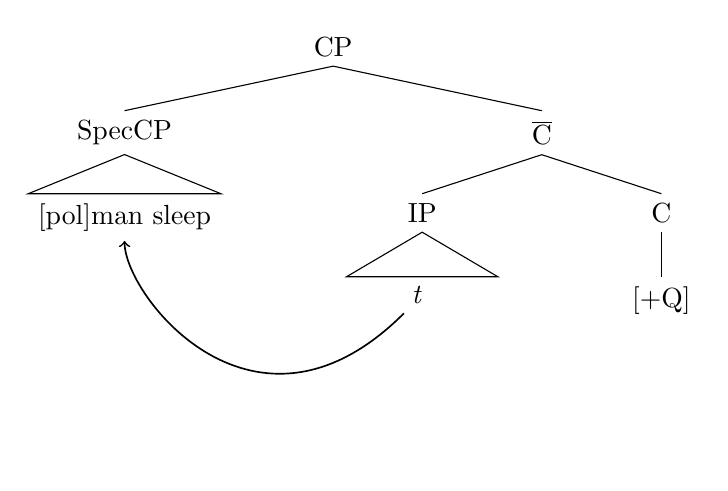
\begin{tikzpicture}[baseline]
\tikzset{level distance=30pt,sibling distance=45pt,every tree node/.style={align=center,anchor=north}}
\Tree [.CP [.SpecCP \edge[roof]; \node(sleepyman){\slg[pol]{man sleep}}; ] [.{$\overline{\textrm{C}}$} [.IP \edge[roof]; \node(t){\qquad \textit{t} \qquad}; ] [.C {$[$+Q$]$} ] ] ]

\draw[semithick,->] (t)..controls +(south west:3) and +(south:1)..(sleepyman);

\end{tikzpicture}
\end{exe}

\noindent Based on \citeauthor{sarac2006interrogative}'s (\citeyear{sarac2006interrogative}) account, declaratives and polar interrogatives only have the same structure superficially (see also \citealt{sarac2007cross}). The latter are, however, the result of the IP being moved to (or being remerged in) SpecCP.

\subsubsection{Syntactic analysis II: \citet{aboh2010sa}}
Finally, I will briefly discuss an idea developed by \citet{aboh2010sa} for (\textit{inter alia}) Sign Language of the Netherlands. Their account is similar to what has been proposed for polar interrogatives in Gungbe (see page \pageref{ex:gungbepolarinterrogativetree}). Although they mainly discuss constituent interrogatives, they propose that Sign Language of the Netherlands has an optional clause-final question particle consisting of the hands being open with palms facing upwards. This sign is usually called `palm-up gesture' (\textsc{p-ug} for short). On their account, \textsc{p-ug} is located in the head of the IntP. 

As their account is strictly antisymmetric, all heads are left-headed and all specifiers are left-branching. As \textsc{p-ug} appears clause-final, they assume that the material located in the IP is obligatorily moved into the specifier of the IntP in polar interrogatives. This not only derives the correct surface order with \textsc{p-ug} clause-finally but also accounts for the fact that the non-manuals are strongest clause-finally as all manual material is then to the left of the Int\textdegree\ that we can easily assume to be the trigger of the non-manual markings.

The difference between the two models is simply that \citet{sarac2006interrogative} assume a right- and \citet{aboh2010sa} a left-headed structure. Under the assumption that the respective head is the trigger of the non-manuals, both models account for the spread of the non-manuals with a clause-final intensity peak.

\subsection{Polar interrogatives in DGS}\label{polarinterrogativesdgs}
In this section, I will first discuss the non-manual markings and their spreading behavior in DGS polar interrogatives and then discuss the use of the palm-up gesture (\textsc{p-ug}) and the behavior of pronoun doubling. I follow earlier proposals that \textsc{p-ug} is located in the head of the IntP \citep{aboh2010sa} and the pronoun double in the head of the FocP \citep{de1999phrase} and show that their order as well as the spreading behavior of the non-manuals can be derived by assuming a right-headed or left-headed account.

\subsubsection{Non-manual markings}
As with other sign languages, the constituent-order in polar interrogatives in DGS is not different from declarative sentences and is thus SOV. The only difference between a declarative and a polar interrogative sentence lies in non-manual marking. With polar questions, signers raise their eyebrows. Additionally, the head is often put forward and tilted (see also \citealt[171--172]{papaspyrou2008grammatik}). While the raising of the eyebrows obligatorily spreads over the whole clause, the forward-stretch of the head as well as the tilting only occurs on the clause-final sign, in most cases on the verb. This is shown exemplarily in Figure \ref{fig:polarint}. The peak of the non-manual markings on the whole can be observed towards the end of the clause.

\begin{figure}[bt]
\centering
	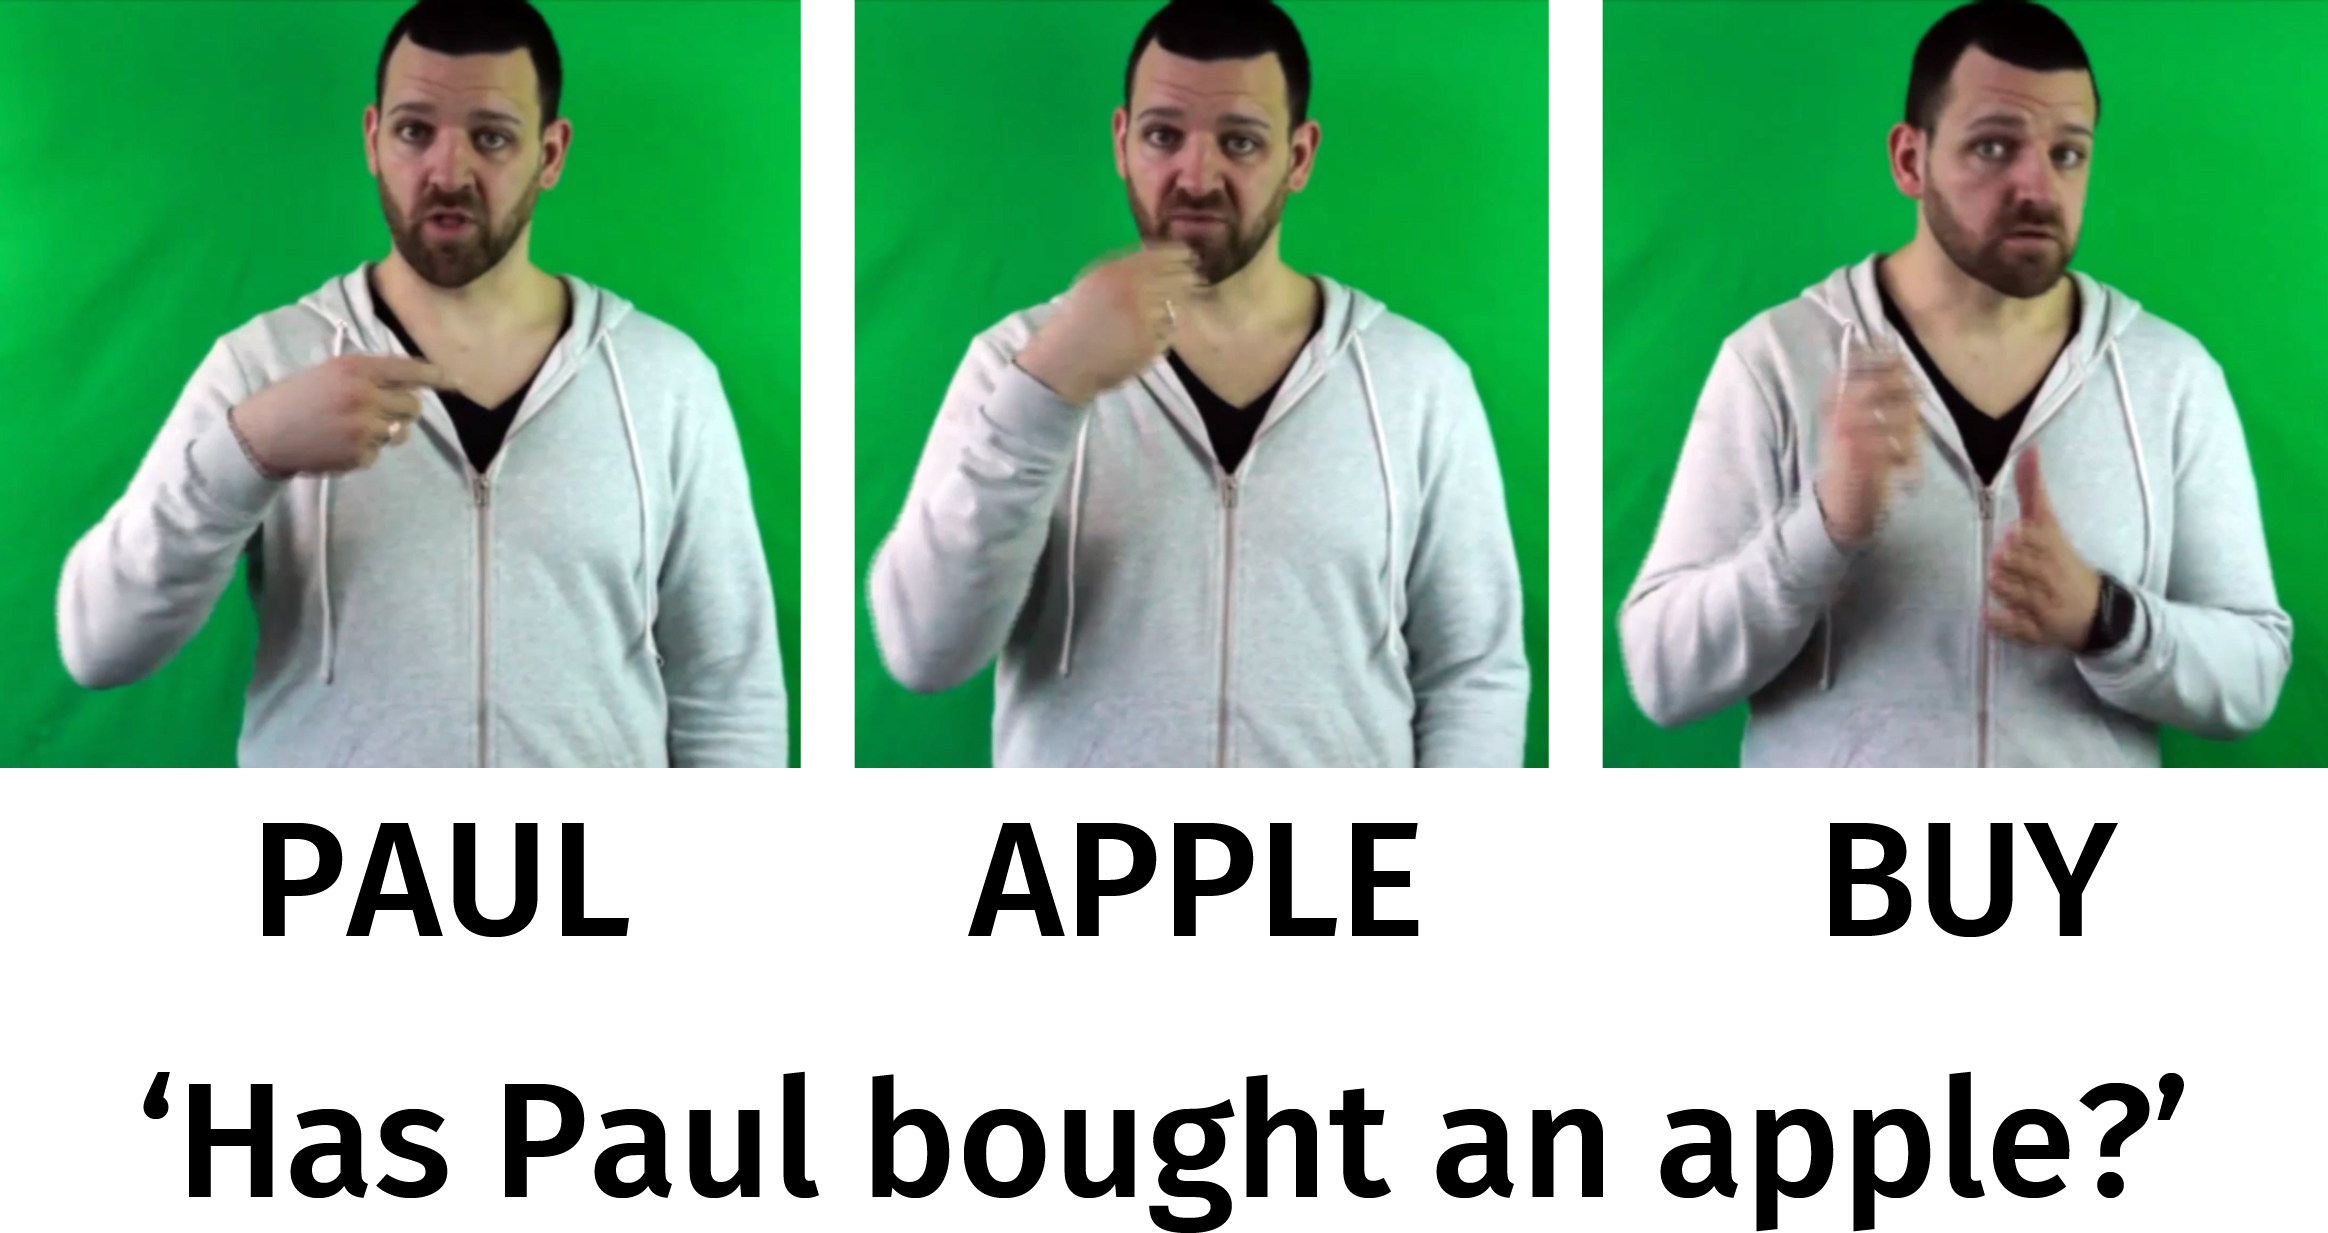
\includegraphics[width=1.0\textwidth]{yesnoquestion.jpg}
	\caption{The non-manuals used in DGS polar interrogatives: raised eyebrows obligatorily spread over the whole clause. Additionally, the clause-final sign is often accompanied by a forward movement of the head and a tilt.}
	\label{fig:polarint}
\end{figure}

Each of the three non-manuals, raising the eyebrows, putting the head forward, and tilting it, fulfills a separate function. While raising the eyebrows is obligatory, the forward movement and the tilt can sometimes be absent. As the brow raise is obligatory, I will take it to be the main non-manual marker responsible for clause-typing. Putting the head forward indicates that the signer awaits a response \citep[171--172]{papaspyrou2008grammatik}. Finally, the head tilt indicates epistemic commitment: the more the head is tilted, the lower the signer's epistemic commitment. In other words: the more the head is put sideways, the more insecure the signer is about the proposition expressed. This explains why it is absent in utterances that only have the surface form of a polar question, such as rhetorical or inclination questions. This is illustrated in Figure \ref{fig:epistemiccommitment} which shows the non-manuals used in a polar question with low epistemic commitment (on the left a screenshot from the question \textit{Can I do an apprenticeship?}) and an inclination question with high epistemic commitment (on the right a screenshot from the question \textit{Can you pass me the salt?}). As the head tilt is not only found in polar interrogatives, but in general is an epistemicity marker, I will discuss it later (see Section \ref{perhapsmoodirrealis} and \ref{rhetq}). Taken together, the three non-manual markers in DGS each fulfill a separate function and can thus be analyzed compositionally.

\begin{figure}[bt]
\centering
	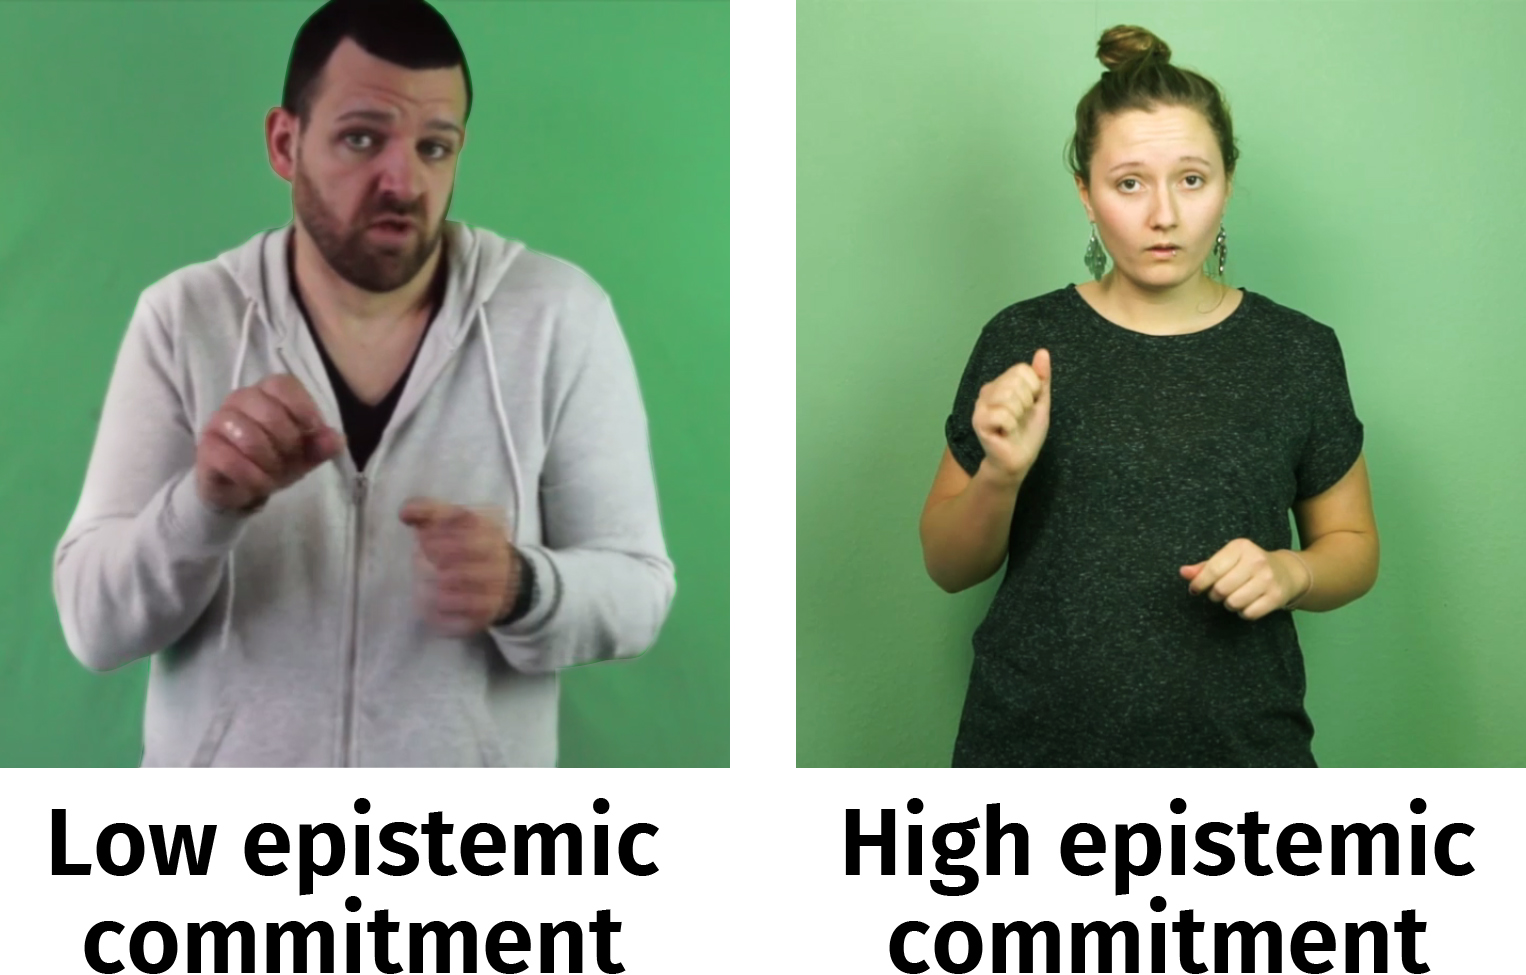
\includegraphics[width=1.0\textwidth]{epistemiccommitment.jpg}
	\caption{Non-manual markings used with polar interrogatives with low and high epistemic commitment. In both cases, the eyebrows are raised and the head is put forward. When the head is additionally tilted to the side as in the picture on the left, the signer signals that s/he is insecure about the proposition. When the head is held straight, in contrast, the signer is confident.}
		\label{fig:epistemiccommitment}
\end{figure}	

\subsubsection{Manual question markers and focus doubling: two possible syntactic analyses}\label{manualquestionmarkers}
That the non-manuals reach their maximum at the end of the clause (this is also true for the raised eyebrows) could be taken as evidence for a right-peripheral interrogative head or, alternatively, as evidence for the fact that the phrase structure below the IntP has moved in an Aboh-\&-Pfau-like manner into SpecIntP as discussed in the previous section for Sign Language of the Netherlands. Using distributional facts of focus and question particles, I will show that both options can be syntactically implemented. Before doing this, I will briefly discuss the use of question particles and focus marking in polar interrogatives in DGS.

Similar to what \citet{aboh2010sa} describe for Sign Language of the Netherlands, it is possible in DGS to make use of an optional clause-final question particle that is extremely similar to the one used in Sign Language of the Netherlands and is usually also glossed \textsc{p-ug}. Its use is illustrated in (\ref{pugpolarintdgs}).

\begin{exe}
\ex \slg[pol]{index\textsubscript{2} can cook p-ug}
%{\hspace{113pt}pol}  \\
%{$\overline{\textrm{\textsc{index}\textsubscript{2} \textsc{can cook p-ug}}}$} 
\glt `Can you cook?'\label{pugpolarintdgs}
\end{exe}

\noindent If \textsc{p-ug} is indeed located in the head of the IntP, the suggestion that all manual material located in the IP in DGS is moved to SpecIntP is a plausible scenario. Alternatively, one might hypothesize that the Int\textdegree\ is right-headed in DGS. 

The\is{focus doubling} same conclusions are to be drawn from the position of focus doubles in DGS. Polar interrogatives, together with imperatives, show a peculiar pattern of pronoun doubling in DGS. In many cases, polar questions with pronoun doubling are not unmarked polar questions. Instead, questions with doubled pronouns often receive emphasis, mainly to indicate that the speaker is surprised (however, this is not necessarily the case. Sometimes pronoun doubling also takes place in regular polar questions). This is illustrated in the following examples.

\vspace{-0.2cm}

\begin{exe}
\ex\label{unmarkedpolarvsdoubling}\begin{xlist}
\ex \slg[pol]{index\textsubscript{2} can cook}
%\ex {\hspace{81pt}pol}  \\
%{$\overline{\textrm{\textsc{index}\textsubscript{2} \textsc{can cook}}}$} %\\
\glt `Can you cook?' \label{ex:unmarkedpolarvsdoublinga}\hfill Regular polar question
\ex \slg[pol]{index_2 can cook \slg[foc]{index\textsubscript{2}}} 
%
%
%\glll   {${\hspace{104pt}\underline{\textrm{\textcolor{white}{lllllll}foc}}}$} \\
%{\hspace{123pt}pol} \\
%{$\overline{\textrm{\textsc{index}\textsubscript{2} \textsc{can cook index}\textsubscript{2}}}$} \\
\glt `YOU can cook?' \label{ex:unmarkedpolarvsdoublingb}\hfill Pronoun doubling

\end{xlist}
\end{exe}

\vspace{-0.2cm}

\noindent Doubling as in (\ref{ex:unmarkedpolarvsdoublingb}) has generally been referred to as `focus doubling' in the literature. The term `focus doubling' is chosen as it is assumed that the clause-final double is located in a focus position, to be more precise in the head of a focus phrase as only heads, but not phrases, can be doubled (e.\,g., \citealt{de1999phrase, sandler2006sign}, but see \citealt{wilbur2012informationstructure} who argues that doubling does not serve as a focus, but as a marker of emphasis). This is in line with the idea that focus is located in a clause-final position in many sign languages (see \citealt{wilbur1991intonation, wilbur1994foregrounding, wilbur1996evidence, wilbur1997prosodic} for American Sign Language). Besides pronouns, other parts of speech can undergo doubling in DGS as well. This is, for example, true for \textit{wh}-signs or modals. 

If the focus double is in the head of FocP, the fact that it occurs clause-finally in DGS is, again, in line with the idea of the IP being moved to SpecIntP or a right-headed Foc\textdegree . Additionally, both modeling possibilities are in line with the fact that the intensity peak of the non-manuals is clause-final in DGS. If taken to the extremes (with all heads and specifiers on the same side), these two modeling possibilities look as depicted in (\ref{ex:polarquestionsanalyis}). 
%\vspace{-0.5cm}
\clearpage
\begin{exe}
\ex\label{ex:polarquestionsanalyis}
\begin{multicols}{2}
\begin{xlist}

\ex \label{ex:polarquestionsanalyisa}
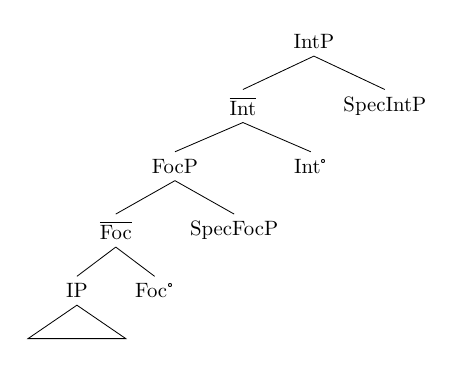
\begin{tikzpicture}[baseline=(current bounding box.north), scale=0.75]
\tikzset{sibling distance=1pt}
\tikzset{every tree node/.style={align=left,anchor=north}}
\Tree [.IntP [.{$\overline{\textrm{Int}}$} [.FocP [.{$\overline{\textrm{Foc}}$} [.IP \edge[roof]; \node(t){\qquad\qquad}; ] [.{Foc\textdegree } ] ] [.SpecFocP ] ] [.{Int\textdegree } ] ] [.SpecIntP ] ]
\end{tikzpicture}


\ex\label{ex:polarquestionsanalyisb}
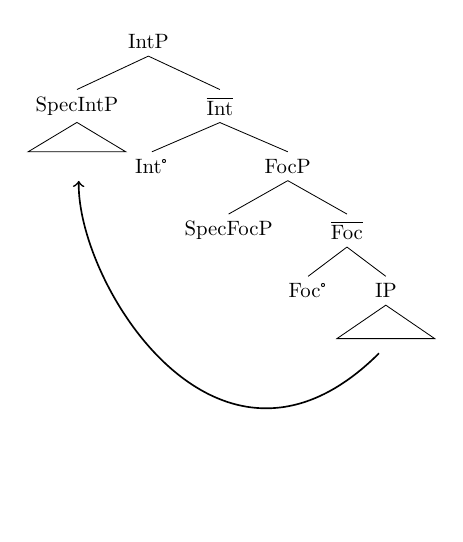
\begin{tikzpicture}[baseline=(current bounding box.north), scale=0.75]
\tikzset{sibling distance=1pt}
\tikzset{every tree node/.style={align=left,anchor=north}}

\Tree [.IntP [.SpecIntP \edge[roof]; \node(specintp){\textcolor{white}{blablabla}}; ] [.{$\overline{\textrm{Int}}$} [.{Int\textdegree } ] [.FocP [.SpecFocP ] [.{$\overline{\textrm{Foc}}$} [.{Foc\textdegree } ] [.IP \edge[roof]; \node(t){\qquad\qquad}; ] ] ] ] ]

\draw[semithick,->] (t)..controls +(south west:4) and +(south:2)..(specintp);



\end{tikzpicture}


\end{xlist}
\end{multicols}
\end{exe}

\vspace{-0.8cm}

\noindent The structure on the left (\ref{ex:polarquestionsanalyisa}) allows specifiers and heads to the right, while the structure on the right (\ref{ex:polarquestionsanalyisb}) shows an anti-symmetric Aboh-\&-Pfau-style structure with all heads and specifiers to the left. To form a polar interrogative, we need to assume movement of the IP material into the specifier of the IntP in the right structure. The non-manuals would then be triggered by spec-head agreement. In the case that a focus double is present, we would assume that it is not only the IP, but the whole FocP that moves to SpecInt. For the model on the left, one would assume an active Int\textdegree\ triggering the non-manuals via c-command without additional movement to SpecInt. In both models, \textsc{p-ug} and focus doubles are predicted to be clause final.

However, the models differ in their prediction of how \textsc{p-ug} and the focus double are ordered. The Aboh-\&-Pfau-style structure predicts that the focus double follows \textsc{p-ug}, while the structure on the right predicts the opposite. What we find is that the question particle \textsc{p-ug} follows rather than precedes the pronoun double in DGS, as shown in (\ref{ex:doublingandpug}) and Figure (\ref{fig:beerbuyyou}).

\begin{exe}
\ex\label{ex:doublingandpug}\begin{xlist}
\ex \textcolor{white}{*}\slg[pol]{index_2 beer buy index_2 p-ug}
%\ex {\hspace{158pt}pol}  \\
%{\textcolor{white}{*}$\overline{\textrm{\textsc{index}\textsubscript{2} \textsc{beer buy index}\textsubscript{2}} \textsc{ p-ug}}$} %\\
\glt \textcolor{white}{*}`Are \textsc{you} buying beer?' \label{ex:doublingandpuga}
\ex *\slg[pol]{index_2 beer buy p-ug index_2}
%\ex {\hspace{158pt}pol}  \\
%{*$\overline{\textrm{\textsc{index}\textsubscript{2} \textsc{beer buy p-ug index}\textsubscript{2}}}$} %\\
\glt \textcolor{white}{*}`Are \textsc{you} buying beer?' \label{ex:doublingandpugb}
\end{xlist}
\end{exe}

\noindent The model on the left in (\ref{ex:polarquestionsanalyis}) can derive a structure like the one in (\ref{ex:doublingandpuga}) as shown in the tree in (\ref{ex:polarquestionsanalyisaaba}).



\begin{exe}
\ex \label{ex:polarquestionsanalyisaaba}
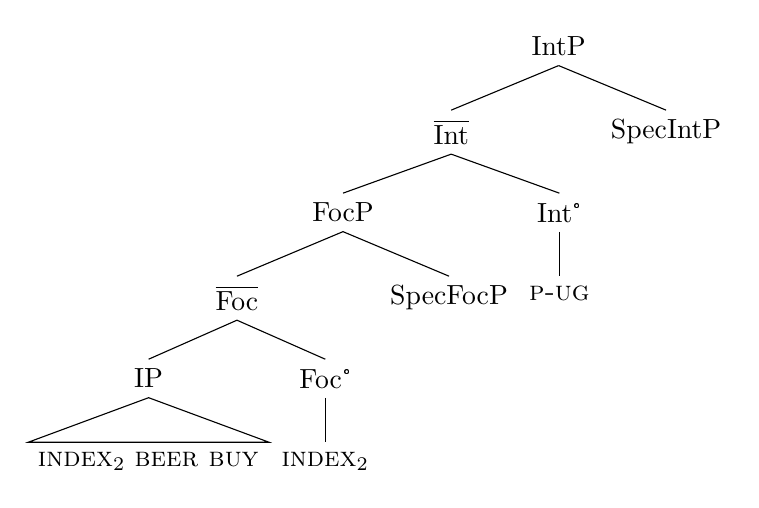
\begin{tikzpicture}[baseline=(current bounding box.north), scale=1.00]
\tikzset{sibling distance=1pt}
\tikzset{every tree node/.style={align=left,anchor=north}}
\Tree [.IntP [.{$\overline{\textrm{Int}}$} [.FocP [.{$\overline{\textrm{Foc}}$} [.IP \edge[roof]; \node(t){\textsc{index}\textsubscript{2} \textsc{beer buy}}; ] [.{Foc\textdegree } {\textsc{index}\textsubscript{2}} ] ] [.SpecFocP ] ] [.{Int\textdegree } {\textsc{p-ug}} ] ] [.SpecIntP ] ]
\end{tikzpicture}

\end{exe}


\begin{figure}[bt]
\centering
	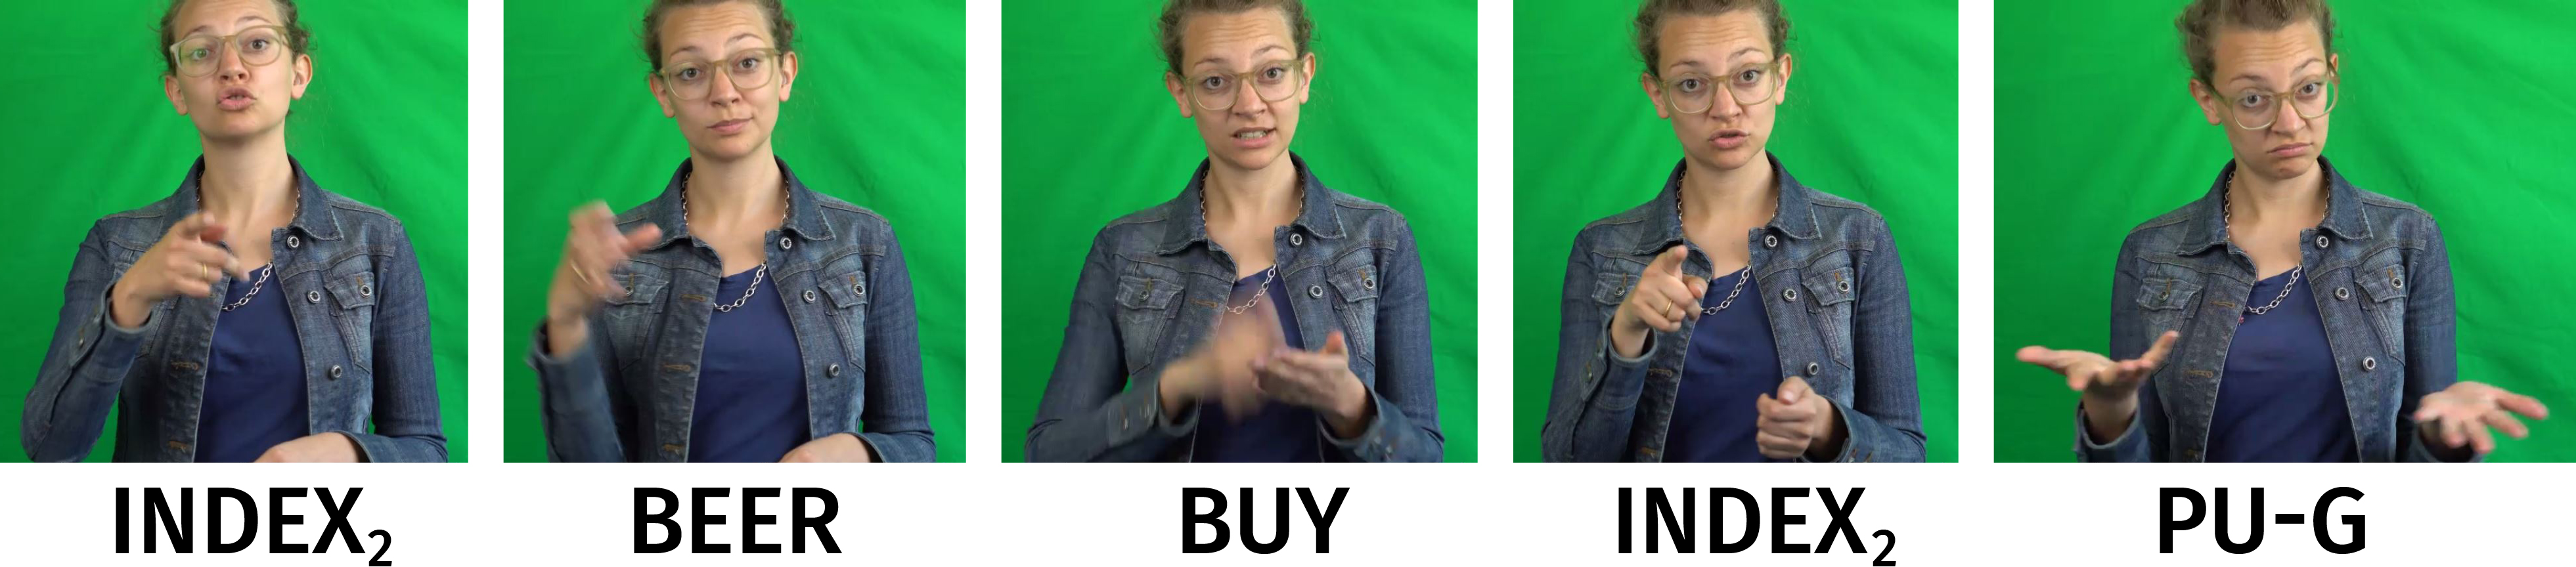
\includegraphics[width=1.0\textwidth]{beerbuyyou.jpg}
	\caption{The palm-up gesture has to follow a focus double in DGS.}
	\label{fig:beerbuyyou}
\end{figure}

\noindent While this model gets rid of the additional movement steps that would be needed in an anti-symmetric model, it is not impossible to derive the correct order in the latter. For this, we would assume that the focus double is moved into Foc\textdegree\ in a first step. Next, the entire IP is moved into SpecFocP and finally, the entire FocP is moved into the specifier of the IntP. This is shown in (\ref{ex:polarquestionsanalyisaababbbb}).


\begin{exe}
\ex \label{ex:polarquestionsanalyisaababbbb}

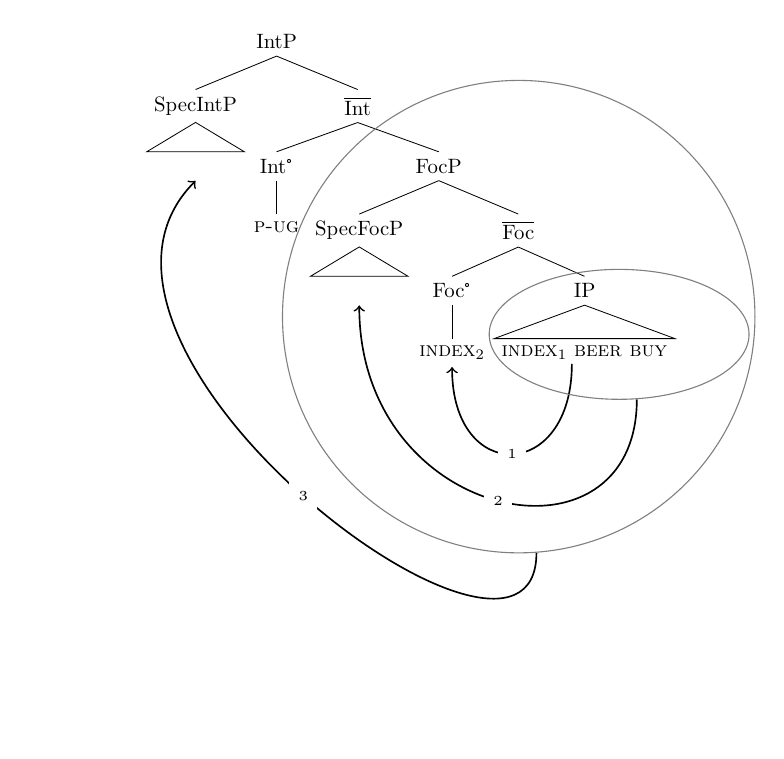
\begin{tikzpicture}[baseline=(current bounding box.north), scale=0.75]
\tikzset{sibling distance=1pt}
\tikzset{every tree node/.style={align=left,anchor=north}}

\Tree [.IntP [.SpecIntP \edge[roof]; \node(specintp){\textcolor{white}{blablabla}}; ] [.{$\overline{\textrm{Int}}$} [.{Int\textdegree } {\textsc{p-ug}} ] [.FocP [.SpecFocP \edge[roof]; \node(specfocp){\textcolor{white}{blablabla}}; ] [.{$\overline{\textrm{Foc}}$} [.{Foc\textdegree } \node(fochead){\textsc{index}\textsubscript{2}}; ] [.IP \edge[roof]; \node(insideip){\textsc{index}\textsubscript{1} \textsc{beer buy}}; ] ] ] ] ]

%\draw[semithick,->] (t.south) to [bend right=-80] node [midway,fill=white] {{\tiny Step 1}} (fochead.south);
%\draw[semithick,->] (insideip)..controls +(west:1) and +(south:2)..(fochead) node [midway,fill=white] {{\small Step 1}};
\draw[semithick, ->] (5,-5.7)..controls +(south:2) and +(south:2)..(fochead.south) node [midway,fill=white] {{\tiny 1}};
\draw[semithick, ->] (6.1,-6.3)..controls +(south:3) and +(south:3.7)..(specfocp.south) node [midway,fill=white] {{\tiny 2}};
\draw[semithick, ->] (4.4,-8.9)..controls +(south:3) and +(south west:4)..(specintp.south) node [midway,fill=white] {{\tiny 3}};
\draw[gray] (5.8,-5.2) ellipse (2.2cm and 1.1cm); %breite and höhe
\draw[gray] (4.1,-4.9) circle (4cm);
\end{tikzpicture}



\end{exe}


\noindent To this end, from the empirical data available, it cannot be decided which derivation is correct. However, the fact that the right-headed structure can explain the clause-final intensity peak of the non-manuals via c-command and is able to derive the right order without any additional movements makes it more likely to be on the right track. %An open question is if \textsc{p-ug} and the  

In the next section, I will discuss constituent interrogatives. Again, I will first introduce the phenomenon and its analyses for spoken languages, then give an overview of the situation found in sign languages, and finally discuss and analyze the situation in DGS.


\is{polar interrogatives|)}

\section{Constituent interrogative sentences}\label{constint}
\is{\textit{wh}-questions|see{constituent interrogatives}
\is{content interrogatives!see{constituent interrogatives}}
\is{constituent interrogatives|(}}

In Section \ref{whgeneral} I will discuss general properties of constituent interrogatives in spoken languages and how they can be analyzed syntactically. I will first discuss the general split of languages exhibiting \textit{wh}-movement and those that do not. Then I will discuss some motivations of \textit{wh}-movement including feature checking and scope-taking. In Section \ref{syntaxoperators}, special attention will be paid to doubling phenomena and the modeling possibilities of languages that have right-peripheral \textit{wh}-phrases as both can be observed in DGS. For this purpose I will discuss, \textit{inter alia}, German \textit{wh}-doubling and and the positions of \textit{wh}-phrases in Northern Italian dialects. From these data I will conclude, following a suggestion made in \citet{aboh2010sa} and \citet{van2010complex, van2012you} that there are several specifier positions in the CP domain hosting \textit{wh}-phrases. 

Section \ref{whsigned} discusses the characteristics of content interrogatives in sign languages and how they were analyzed in the literature. In Section \ref{whinterrogativedgs} I will discuss content interrogatives in DGS and how \textit{wh}-movement in this language can be modeled. From the distribution of \textit{wh}-phrases in the DGS clause and doubling possibilities, I will show  that \textit{wh}-phrases in DGS obey the same restrictions as \textit{wh}-phrases in German and Northern Italian. Again, it will be argued that it is possible to derive the data by an account that allows specifiers and heads on either side as well as in an antisymmetric manner. As with polar interrogatives, in an antisymmetric model additional movement steps have to be assumed. 


\subsection{General overview}\label{whgeneral}
\subsubsection{\textit{Wh}-movement}
Languages fall into two broad classes when it comes to constituent interrogative sentences. While some languages, like English, overtly move \textit{wh}-phrases to the left periphery, other languages, like Mandarin Chinese, leave \textit{wh}-elements \textit{in-situ}. Many theories assume that the movement of the \textit{wh}-element in \textit{in-situ} languages also takes place, but only at LF (e.\,g., \citealt{rizzi1990relativized,cheng1997typology}). The motivation of this movement is standardly assumed to be driven by feature checking. This means that there is a high CP head containing a $[+$wh$]$-feature that is checked by moving a \textit{wh}-phrase into its specifier. Additionally, it is sometimes assumed that there is the need to check an $[+$int$]$ feature, just like in polar interrogatives. That $[+$int$]$ feature checking also applies to constituent interrogatives is backed up by the observation that both question types involve auxiliary inversion in English. However, subject-auxiliary inversion is absent in many languages. It is thus sometimes assumed that \textit{wh}-movement itself can serve for clause-typing \citep{cheng1997typology}. 

Note that \textit{wh}-phrases are quantifiers. So a simple question like \textit{Who bought beer?} can informally be rephrased as: `For which \textit{x}, \textit{x} being a person, is it true that \textit{x} bought a beer'. From this loose rephrasing it becomes apparent that a \textit{wh}-phrase (or the Q-head) is an operator binding a variable. To bind its variable, a \textit{wh}-operator must take scope over the rest of the clause. Thus, instead of assuming that \textit{wh}-movement is driven by feature checking, an alternative would be to say that \textit{wh}-phrases move for scope-taking purposes. I will return to the motivation for \textit{wh}-movement in a moment, but will first make a brief remark on the -- interwoven -- question of where \textit{wh}-phrases move to. 

\label{abohpfaua}
On many accounts, \textit{wh}-phrases move into the specifier of a focus projection FocP (e.\,g., \citealt{rizzi2001position}). This is plausible as \textit{wh}-phrases are, at least in many cases, focused. Such an analysis is unproblematic as long as it is not assumed that movement to SpecFocP is responsible for clause-typing (via feature checking) since FocP is a focus projection and should not bear any interrogative features -- as there are cases in which an element moves to the focus projection, but the clause does not end up being interrogative. There are different ways to solve this. One could either abandon the idea of SpecFocP being the landing site of \textit{wh}-movement or maintain the idea, but assume that there is an additional movement step involved. The latter idea is pursued, for example, by \citet{aboh2010sa} that I will discuss in the following paragraphs.

\subsubsection{Unifying polar and constituent interrogatives and the landings sites of \textit{wh}-phrases}
\citet{aboh2010sa} assume that different types of \textit{wh}-phrases have different landing sites. To unify polar and constituent interrogatives, they additionally argue that clause-typing involves InterP in both polar and constituent interrogatives, and that \textit{wh}-movement does not result from feature checking for the purpose of clause-typing, but rather from the structural make-up of the \textit{wh}-phrase. In the following, I will briefly review their evidence.

That \textit{wh}-phrases target different positions in the clausal-spine becomes clear in languages like Bulgarian that allow the movement of several \textit{wh}-phrases into the left periphery \citep{rudin1988multiple}. As it is only possible to move several \textit{wh}-phrases in a strict order, several distinct landing sites need to be assumed -- even under the assumption that one \textit{wh}-phrase lands in the specifier of FocP, there need to be several landing sites for \textit{wh}-movement. 

However, in languages that do not allow moving more than one \textit{wh}-phrase, there is also evidence that different \textit{wh}-phrases target different positions. This can be seen, for example, in French. The examples in (\ref{adjunctargumentwhphrases}) from \citet[101]{aboh2010sa} show that adjunct and subject \textit{wh}-phrases in French behave differently from object \textit{wh}-phrases regarding their position relative to a topic.

\begin{exe}
\ex French \citep[101]{aboh2010sa}\label{adjunctargumentwhphrases}\begin{xlist}
\ex \gll {\cmark /?\textit{Comment,}} {\textit{demain,}} {\textit{ferons-nous}} {\textit{face}} {\textit{à}} {\textit{cette}} {\textit{nouvelle}} {\textcolor{white}{\cmark /?}\textit{crise ?}} \\
{\textcolor{white}{\cmark /?}how} {tomorrow} {do.\textsc{fut}-\textsc{1pl}} {face} {to} {that} {new} {\textcolor{white}{\cmark /?}crisis}\\
\trans \textcolor{white}{\cmark /?}`How are we going to face this new crisis tomorrow?' \label{adjunctargumentwhphrasesa}

\ex \gll {\cmark /?\textit{Qui,}} {\textit{demain,}} {\textit{dirigera}} {\textit{la}} {\textit{France ?}}  \\
{\textcolor{white}{\cmark /?}who} {tomorrow} {rule-over.\textsc{fut}} {the} {France}\\
\trans \textcolor{white}{\cmark /?}`Who will rule over France tomorrow?'\label{adjunctargumentwhphrasesb}

\ex \gll {\textcolor{white}{\cmark /}*\textit{Qui,}} {\textit{demain,}} {\textit{inviterons-nous ?}}   \\
{\textcolor{white}{\cmark /?}who} {tomorrow} {invite.\textsc{fut}-\textsc{1pl}} \\
\trans \textcolor{white}{\cmark /?}`Who are we inviting tomorrow?'\label{adjunctargumentwhphrasesc}

\end{xlist}
\end{exe}

\noindent While French native speakers accept an adjunct \textit{wh}-phrase being moved into a position higher than the topic (in the examples \textit{demain} `tomorrow'), as shown in (\ref{adjunctargumentwhphrasesa}) and also a subject \textit{wh}-phrase (\ref{adjunctargumentwhphrasesb}), the same is not true for object \textit{wh}-phrases, as illustrated in (\ref{adjunctargumentwhphrasesc}) (note that Aboh \& Pfau report that some speakers accept the sentences in (\ref{adjunctargumentwhphrasesa}) and (\ref{adjunctargumentwhphrasesb}) and some rated them as being marginal). \citet[102]{aboh2010sa} conclude that there are different landing sites, at least for adjunct, subject, and object \textit{wh}-phrases that are ordered in the way represented in (\ref{adbohpfauwhordering}).

\begin{exe}
\ex $[$Wh\textsubscript{adjunct} \dots\ Wh\textsubscript{subject} \dots\ Topic \dots Wh\textsubscript{object} \dots\  $[$IP \dots $]$$]$ \label{adbohpfauwhordering}
\end{exe}

\noindent Given the fact that the landing site of \textit{wh}-movement is, in some languages, the focus projection, and the fact that some languages seem to have different landing sites for different \textit{wh}-phrases the hypothesis that \textit{wh}-movement is responsible for clause-typing becomes unlikely. \citet{aboh2010sa} thus dissociate focus and \textit{wh}-features from clause-typing in constituent interrogative clauses. Instead, they claim that constituent questions involve an IntP responsible for clause typing. Additionally, they assume that the head of IntP is left unexpressed in many languages. \citet{aboh2010sa}, however, speculate that the null Inter head correlates with a special intonation that accompanies \textit{wh}-questions in many spoken languages.

Indeed, there are languages that exhibit an overt question particle even in \textit{wh}-questions which supports the view that there is an Inter\textdegree\ present not only in polar, but also in constituent interrogatives. \citet{aboh2010sa} cite the Niger-Congo language Lele. An example of a Lele \textit{wh}-question is given in (\ref{lelewhquestion}), taken from \citet[286]{frajzyngier2001grammar}.


\begin{exe}
\ex Lele \citep[286]{frajzyngier2001grammar} \\ \gll {\textit{Me}} {\textit{ba}} {\textit{gol}} {\textit{dí}} {\textit{gà?}} \\
{What} {\textsc{foc}} {see} {3.\textsc{sg}} {\textsc{inter}} \\
\trans `What did he see?' \label{lelewhquestion}
\end{exe}

\noindent Lele, a mixed \textit{wh}-movement language, moves the \textit{wh}-phrase into the left-peripheral focus projection, as can been seen by the position of the \textit{wh}-phrase to the left of the focus marker \textit{ba} in the example. At the same time, the question is marked by the clause-final question marker \textit{gà} that is taken to be responsible for clause-typing by \citet{aboh2010sa}. On their account, the question marker is located in the head of the InterP in the left periphery. That it appears in a clause-final position is derived through movement of the material that is located below FocP. This is illustrated in (\ref{ex:lelederivationabohpfau}).

\begin{exe}
\ex\label{ex:lelederivationabohpfau} 
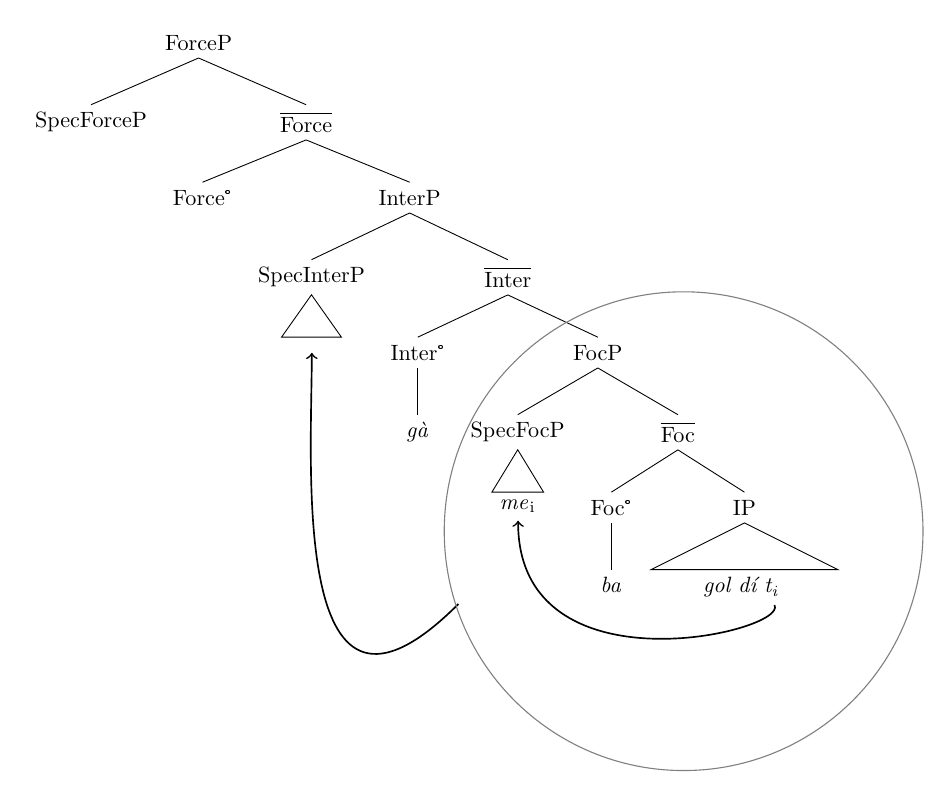
\begin{tikzpicture}[baseline=(current bounding box.north), scale=0.80]
\tikzset{level distance=35pt,sibling distance=5pt,every tree node/.style={align=center,anchor=north}}
%\Tree [.ForceP [.{SpecForceP} ] [.{$\overline{\textrm{Force}}$} [.{Force\textdegree } ] [.InterP [.SpecInterP \edge[roof]; \node(sleepyman){S\'{\textepsilon }t\`{\textopeno } k\`{o} w\^{a}?}; ] [.{$\overline{\textrm{Inter}}$} [.{Inter\textdegree } {$[+$interrogative$]$} ] [.TopP [.SpecTopP ] [.{$\overline{\textrm{Top}}$} [.{Topic\textdegree } ] [.FocP [.SpecFocP ] [.{$\overline{\textrm{Foc}}$} [.{Foc\textdegree } ] [.IP \edge[roof]; \node(t){\qquad \textit{t} \qquad}; ] ] ] ] ] ] ] ] ]
\Tree [.ForceP [.SpecForceP ] [.{$\overline{\textrm{Force}}$} [.{Force\textdegree} ] [.InterP [.SpecInterP \edge[roof]; \node(sleepyman){\qquad }; ] [.{$\overline{\textrm{Inter}}$} [.{Inter\textdegree} {\textit{gà}} ] [.FocP [.SpecFocP \edge[roof]; \node(me){\textit{me}\textsubscript{i}}; ] [.{$\overline{\textrm{Foc}}$} [.{Foc\textdegree } {\textit{ba}} ] [.IP \edge[roof]; \node(t){\qquad \textit{\textit{gol dí t\textsubscript{i}}} \qquad}; ] ] ] ] ] ] ]
\node (A) at (4.28,-9) {};
\draw[semithick,->] (A)..controls +(south west:4) and +(south:2)..(sleepyman);
%\draw[semithick,->] (A.south) to [bend right=-80] node [midway,fill=white] {Step 1} (sleepyman.south);
\draw[semithick,->] (t)..controls +(south east:1) and +(south:3)..(me);
\draw[gray] (7.7,-8) circle (3.8cm);
\end{tikzpicture}
\end{exe}

\noindent What the tree structure shows is that \citet{aboh2010sa} assume that the \textit{wh}-word \textit{me} first moves into the specifier of the focus phrase and then the whole proposition, i.\,e., everything below the FocP (marked by the circle), moves into the specifier of the interrogation phrase. To summarize: \citet{aboh2010sa} generally suggest to dissociate \textit{wh}-movement from clause-typing. They assume that \textit{wh}-movement happens for focus feature checking purposes while setting the interrogative force is done in InterP (in polar as well as in \textit{wh}-interrogatives).\footnote{ Note that \citet{aboh2010sa} suggest that intonation (in spoken languages) and non-manual markings (in sign languages) are indicators of the Inter\textdegree . On the assumption that the interrogative force in polar and constituent questions is the same, we need to ask why there are so many spoken languages with different intonational patterns in polar and constituent interrogatives and so many sign languages with different non-manual markers for the same distinction.} 

\subsection{The notion of `syntactic operators' and \textit{wh}-copying}\label{syntaxoperators}
\subsubsection{Simple and complex \textit{wh}-phrases}
While it is not possible to move several \textit{wh}-phrases into the left periphery in English, it is well-known that the choice of the \textit{wh}-element to be moved is not random. Instead, the \textit{wh}-phrase which is closest to SpecCP has to move while all other \textit{wh}-phrases need to stay \textit{in-situ}. This phenomenon, known under the labels `Superiority Effect', `Shortest Move Principle', or `Attract Closest', is illustrated in (\ref{againshortestmoveaaa}) and (\ref{againshortestmoveaab}). While the sentence in (\ref{againshortestmoveaaa}) is well-formed given that the subject-\textit{wh}-phrase is moved as it is structurally closer to SpecCP (or the head attracting it), moving the structurally lower object-\textit{wh}-phrase to SpecCP (or whatever its exact landing site may be), as in (\ref{againshortestmoveaab}) violates the Shortest Move Principle and leads to an ill-formed structure.

\begin{exe}
\ex\label{againshortestmove}\begin{xlist}
\ex \textcolor{white}{*}Who will drink what? \label{againshortestmoveaaa}
\ex *What will who drink? \label{againshortestmoveaab}
\end{xlist}
\end{exe}

\noindent Although this generalization is very stable, it has long been recognized that there are some exceptions, as shown in (\ref{againshortestmoveaac}) (this was first observed in a series of unpublished papers by \citealt{reinhart1986mimeo, reinhart1987mimeo, reinhart1990mimeo}).

\begin{exe}
\ex \textcolor{white}{*}What did which student drink? \label{againshortestmoveaac}
\end{exe}

\noindent While the \textit{wh}-question in (\ref{againshortestmoveaab}) is ill-formed because the object-\textit{wh}-element \textit{what} does not obey the Shortest Move Principle, the structure in (\ref{againshortestmoveaac}) is fine, although the same movement operation took place, as in both cases, (\ref{againshortestmoveaab}) and (\ref{againshortestmoveaac}), it is the object-\textit{wh}-phrase that is being preposed. The only difference between the two is that the ill-formed structure involves a simple (\textit{who}) and the well-formed structure a complex \textit{wh}-phrase (\textit{which student}). A similar contrast is shown in (\ref{againshortestmovea}), from \citet[4--5]{reinhart1990mimeo}. This minimal pair illustrates that simple \textit{wh}-adjuncts are not well-formed \textit{in-situ} in a \textit{wh}-island (\ref{againshortestmoveaa}), but complex \textit{wh}-phrases are (\ref{againshortestmoveab}). 

\begin{exe}
\ex\label{againshortestmovea}\begin{xlist}
\ex *Who fainted when you behaved how? \label{againshortestmoveaa}
\ex \textcolor{white}{*}Who fainted when you behaved which way? \label{againshortestmoveab}
\end{xlist}
\end{exe}

\noindent Following \citet{van2010complex}, I argue that simple \textit{wh}-phrases, like \textit{who}, \textit{what}, or \textit{how}, are syntactic operators while at least some complex \textit{wh}-phrases are not (see also \citealt{cinque1986bare, pesetsky1987wh, dobrovie1990clitic, grewendorf2012wh}). Thus, while the movement of \textit{what} into a scope-taking position is blocked in (\ref{againshortestmoveaab}) because of the intervening operator \textit{who}, the same movement is not blocked in (\ref{againshortestmoveaac}), as the complex \textit{wh}-phrase \textit{which student} is not an operator and thus does not intervene. In other words: \textit{wh}-phrases in English move into the left periphery to take scope over the clause. When two or more \textit{wh}-phrases are present in a clause, the structurally highest \textit{wh}-phrase that is a syntactic operator is moved and the lower ones remain \textit{in-situ} (at least at PF).  

Despite their different behavior in multiple \textit{wh}-questions, both simple and complex \textit{wh}-phrases are able to type a clause as a \textit{wh}-question (if one assumes that \textit{wh}-movement is involved in clause-typing) and both are able to create operator-variable dependencies. Without going into too much detail, I quickly illustrate that both simple and complex \textit{wh}-phrases show the typical properties of operator-variable dependencies in (\ref{weakcrossoversimplecomplexwh}) and (\ref{parasiticgapssimplecomplexwh}), both from \citet[240]{van2010complex}. The examples in (\ref{weakcrossoversimplecomplexwh}) illustrate that both are sensitive to weak crossover effects and (\ref{parasiticgapssimplecomplexwh}) shows that both can license parasitic gaps.

\begin{exe}
\ex\label{weakcrossoversimplecomplexwh}\begin{xlist}
\ex *Who\textsubscript{i} does his\textsubscript{i} mother like \textit{t}\textsubscript{i} \label{weakcrossoversimplecomplexwha}
\ex *Which boy\textsubscript{i} does his\textsubscript{i} mother like $\textrm{\textit{t}}$\textsubscript{i} \label{weakcrossoversimplecomplexwhb}
\end{xlist}
\end{exe}

\begin{exe}
\ex\label{parasiticgapssimplecomplexwh}\begin{xlist}
\ex \textcolor{white}{*}What\textsubscript{i} did you file \textit{t}\textsubscript{i} without reading \textit{e}\textsubscript{i}? \label{parasiticgapssimplecomplexwha}
\ex \textcolor{white}{*}Which book\textsubscript{i} did you file \textit{t}\textsubscript{i} without reading \textit{e}\textsubscript{i}? \label{parasiticgapssimplecomplexwhb}
\end{xlist}
\end{exe}

\noindent To account for these facts, \citet{van2010complex, van2012you} proposes to split up the CP into two projections, one responsible for clause-typing, called CP\textsubscript{1}, and one for creating operator-variable dependencies, called CP\textsubscript{2}. While CP\textsubscript{1} contains a question feature, CP\textsubscript{2} contains an operator feature. This is illustrated in (\ref{ex:vancaenenbroekone}).

\begin{exe}
\ex\label{ex:vancaenenbroekone} 
\begin{tikzpicture}[baseline]
\tikzset{level distance=30pt,sibling distance=50pt,every tree node/.style={align=center,anchor=north}}
\Tree [.{CP\textsubscript{1}} [.{} ] [.{$\overline{\textrm{C\textsubscript{1}}}$} [.{C\textsubscript{1}\textdegree \\ $[$+Q$]$} ] [.{CP\textsubscript{2}} [.{} ] [.{$\overline{\textrm{C\textsubscript{2}}}$} [.{C\textsubscript{2}\textdegree \\ $[$+Op$]$} ] [.IP \edge[roof]; \node(t){\textcolor{white}{nancy buy}}; ] ] ] ] ]
%\Tree [.CP [.SpecCP \edge[roof]; \node(what){\textsc{what}}; ] [.{$\overline{\textrm{C}}$} [.IP \edge[roof]; \node(t){\textsc{nancy buy} \textit{t} \textsc{yesterday}}; ] [.{C\textdegree \\ $[+$focus$]$ \\ $[$+wh$]$} [.\node[draw=gray,circle]{\textsc{what}}; ] ] ] ]
%\draw[semithick,->] (t)..controls +(south west:4) and +(south:2)..(what);
%
%\node[draw=white,text=gray] at (6.5,-9.3) {\large base-generated};
%\node[draw=white,text=gray] at (6.5,-9.8) {\large double};
\end{tikzpicture}
\end{exe}

\noindent Note that splitting up the CP in this way is rather uncontroversial as it is generally assumed that the CP consists of a whole array of functional projections \citep{rizzi1997fine, rizzi2001position}. Similar accounts can be found all over the literature (e.\,g., \citealt{poletto2002left, zanuttini2003eclamative}). In fact, it resembles the proposal by \citet{aboh2010sa} of splitting up the CP into several projections that can host different types of \textit{wh}-phrases (see the previous subsection).

On van Craenenbroek's account, simple \textit{wh}-phrases move via SpecCP\textsubscript{2} to SpecCP\textsubscript{1} to check both the operator and the clause-typing feature. Complex \textit{wh}-phrases are base-generated in SpecCP\textsubscript{1} only checking the clause-typing feature while the operator feature is checked via \label{emptyoperator}empty operator movement from within the IP to SpecCP\textsubscript{2}. Splitting up the CP in this way makes sense for at least two reasons. First, from a Cartographic perspective it is desirable to assume that two distinct functions are represented in two heads (see the discussion of the One Feature One Head Principle on page \pageref{ofoh}). Second, the fact that simple \textit{wh}-phrases behave differently from complex \textit{wh}-phrases in multiple \textit{wh}-questions has to be accounted for in some way.

\subsubsection{\textit{Wh}-copying in German}
Crucially, simple and complex \textit{wh}-phrases actually behave differently not only in multiple \textit{wh}-interrogatives, but in a number of others constructions in various languages. Of special interest for the purpose of the present study are \textit{wh}-copying phenomena as these constructions show that the split between \textit{wh}-phrases being operators and \textit{wh}-phrases not being operators is not a split between simple and complex \textit{wh}-phrases, but a split between simple \textit{wh}-phrases and \textit{wh}-phrases contained in a PP on the one hand and complex \textit{wh}-phrases on the other: while many complex \textit{wh}-phrases do not allow copying, presumably because they are not operators, simple \textit{wh}-phrases, as well as \textit{wh}-PPs, do. One language in which such \textit{wh}-copying phenomena are found is German.

The phenomenon under discussion concerns long-distance movement of \textit{wh}-phrases out of an embedded clause into the left-periphery of a matrix clause. In this kind of construction, German allows an overt copy of the moved \textit{wh}-phrase in the left edge of the embedded clause, as illustrated in (\ref{whcopyinggerman}) -- although the sentences are interpreted as containing only one \textit{wh}-phrase. Note that it is also possible in German to only spell out the higher copy.\footnote{ I will not discuss examples of sentences with only the higher copy spelled out. However, for a true understanding of this phenomenon it would be necessary to take into account that when only the higher copy is spelled out additional verb movement is required (the example in (\ref{ex:whcopyinggermanb}), with one copy would be \textit{Was glaubst du, kauft er?}). This, however, is unproblematic for the current analysis.\label{footnotewh}} 

\begin{exe}
\ex German\label{whcopyinggerman}\begin{xlist}
\ex \gll {Wer} {\textit{glaubst}} {\textit{du},} {wer} {\textit{gewinnt}?} \\
{who} {believe} {you} {who} {wins}\\
\trans `Who do you think will win?' \label{ex:whcopyinggermana}
\ex \gll {Was} {\textit{glaubst}} {\textit{du},} {was} {\textit{er}} {\textit{kauft}?} \\
{what} {believe} {you} {what} {he} {buys}\\
\trans `What do you think will he buy?' \label{ex:whcopyinggermanb}
\ex \gll {Wie} {\textit{denkst}} {\textit{du},} {wie} {\textit{es}} {\textit{ausgeht}?} \\
{how} {think} {you} {how} {it} {ends}\\
\trans `How do you think it will end?' \label{ex:whcopyinggermanc}
\end{xlist}
\end{exe}

\noindent The traditional analysis of this kind of data is that the spelled out copy (i.\,e., the lower one) is left behind by a sucessive cyclic upward movement (\citealt{mcdaniel1986conditions, fanselow2000towards, hohle2000w, nunes2004linearization, schippers2012some, pankau2013replacing, bayer1984comp, bayer2014}). Interestingly, this construction is only possible with \textit{wh}-operators and is thus banned with complex \textit{wh}-phrases, as shown in (\ref{whcopyinggermana}) -- a situation that parallels the restrictions of English multiple \textit{wh}-question formation as the grammaticality contrasts also arise through the difference between simple and complex \textit{wh}-phrases (and as I will discuss later, it also parallels the situation found in many sign languages).





\begin{exe}
\ex German \label{whcopyinggermana} \begin{xlist}
\ex \gll {*Welches} {Auto} {\textit{denkst}} {\textit{du},} {welches} {Auto} {\textit{Otto}} {\textit{kauft}?}   \\
{\textcolor{white}{*}which} {car} {think} {you} {which} {car} {Otto}  {buys}\\
\trans \textcolor{white}{*}`Which car do you think will Otto buy?' \label{ex:whcopyinggermanaa}\ex \gll  {*Wessen}  {Auto}  {\textit{meinst}}  {\textit{du},}  {wessen}  {Auto}  {\textit{das}}  {\textit{ist}?} \\
{\textcolor{white}{*}whose} {car} {think} {you} {whose} {car} {that} {is} \\
\trans \textcolor{white}{*}`Whose car do you think that is?' \label{ex:whcopyinggermanab}
\end{xlist}
\end{exe}

\noindent On \citeauthor{van2010complex}'s (\citeyear{van2010complex, van2012you}) account, the ill-formedness of the examples in (\ref{whcopyinggermana}) is a direct consequence of the complex \textit{wh}-phrases being base-generated in (the structurally higher) CP\textsubscript{1}. Thus, it is not possible to spell out a copy in the embedded clause, simply because there is no such copy (note that the examples would be well-formed if only the first instances of the \textit{wh}-phrases would be present; cf. Footnote \ref{footnotewh}). Crucially, however, this construction is only banned with complex \textit{wh}-phrases that behave in a non-operator way and works quite well with those that do not -- and for some reason to be explored, it is not only simple \textit{wh}-phrases that behave like operators, but also \textit{wh}-phrases contained in a PP. This is illustrated in (\ref{whcopyinggermanb}). Note that I marked the construction as being marked -- but crucially, it is not ill-formed.\footnote{ Some authors (e.\,g., \citealt{felser2004wh}) mark similar examples as being marked, while others do not (e.\,g., \citealt{van2010complex}). Indeed, some German speakers find examples like the ones in (\ref{whcopyinggermanb}) totally natural, while others perceive them as a little marked. I think the reason for the different judgments is that this phenomenon is restricted to colloquial speech styles.}

\begin{exe}
\ex Colloquial German\label{whcopyinggermanb}\begin{xlist}
\ex \gll {\%{Mit}} {wem} {\textit{glaubst}} {\textit{du},} {mit} {wem} {\textit{er}} {\textit{sich}} {\textit{trifft}?}   \\
{\textcolor{white}{\%}with} {who} {think} {you} {with} {who} {he} {\textsc{refl}}  {\textit{meet}}\\
\trans \textcolor{white}{\%}`Who do you think is he meeting with?' \label{ex:whcopyinggermanba}
\ex \gll {\%{Auf}} {wen} {\textit{glaubst}} {\textit{du},} {auf} {wen} {\textit{er}} {\textit{sauer}} {\textit{ist}?}  \\
{\textcolor{white}{\%}at} {who} {think} {you} {at} {who} {he} {angry} {is} \\
\trans \textcolor{white}{\%}`At whom do you think he is angry?' \label{ex:whcopyinggermanbb}

\end{xlist}
\end{exe}

\noindent The examples show that it is indeed possible to copy a complex \textit{wh}-phrase in German \textit{wh}-copying constructions \citep{mcdaniel1986conditions, felser2004wh, nunes2004linearization, van2010complex}. This is, however, only true for PPs containing a \textit{wh}-phrase, like \textit{mit X} `with X', \textit{auf X} `at X', or \textit{für X} `for X'.\footnote{ There are, as already noted, many languages for which there is evidence that simple \textit{wh}-phrases pattern together with \textit{wh}-phrases contained in a PP and that the former two behave differently from complex \textit{wh}-phrases. Due to reasons of space I will only discuss data from German and Italian. For more evidence for the different behavior of simple and complex \textit{wh}-phrases see the data from English, Frisian, German, Afrikaans, and Dutch in \citet{van2010complex, van2012you} and \citet{felser2004wh}. Additionally, I refer the reader to \citet{mcdaniel1986conditions, mcdaniel1989partial} for data from Romani to \citet{de1990acquisition}, \citet{thornton1990adventures}, \citet{thornton1999levels}, and \citet{mcdaniel1995parameters} for enlightening data from child English in which sentences with simple \textit{wh}-phrases often show copying like in (\ref{childrensenglisha}), while the same phenomenon with complex \textit{wh}-phrases is not found (\ref{childrensenglishb}). Instead children produce sentences like (\ref{childrensenglishc}) (examples from \citealt[7]{thornton1999levels}).

\begin{exe}
\ex\label{childrensenglish}\begin{xlist}
\ex \textcolor{white}{*}Who do you think who's in the box? \label{childrensenglisha}
\ex *Which Smurf do you think which Smurf is hiding in the box? \label{childrensenglishb}
\ex \textcolor{white}{*}Which guys did they guess which had the ants in the their pants? \label{childrensenglishc}
\end{xlist}
\end{exe}



}  

While it is clear that a more elaborated analysis of the presented data is needed, the crucial point is that there are some complex \textit{wh}-phrases that do not behave as syntactic operators (especially the \textit{which}-N and \textit{whose}-N construction) and others that do (PP-\textit{wh}-phrases, e.\,g., \textit{with whom}). 

\subsubsection{Do simple \textit{wh}-phrases always move to SpecCP\textsubscript{1}?}
The idea of splitting up the CP in order to provide more space for \textit{wh}-elements in fact lines up very well with the account by \citet{aboh2010sa} presented in the preceding subsection. Irrespective of labels it can also account for the fact that in some languages it is possible to have two complementizers and a \textit{wh}-phrase in one clause. This is illustrated for colloquial Dutch in (\ref{colloquialdutchcraenenbroekzweitausenddreizehn}), taken from \citet[45]{van2012you}.

%\clearpage

\begin{exe}
\ex Colloquial Dutch \citep[45]{van2012you} \\ \gll {\textit{Ik}} {\textit{vraag}} {\textit{me}} {\textit{af}} {\textit{wie}} {of} {dat} {\textit{je}} {\textit{zoekt}.}  \\
{I} {ask} {me} {\textsc{prt}} {who} {if} {that} {you} {seek} \\
\trans `I wonder who you are looking for.' \label{colloquialdutchcraenenbroekzweitausenddreizehn}

\end{exe}

\noindent If we assume, following \citet{van2012you}, that the complementizer \textit{of} `if' occupies the head of CP\textsubscript{1} and that \textit{dat} `that' sits in the head of CP\textsubscript{2}, we arrive at the representation shown in (\ref{ex:vancaenenbroekonea}).

\begin{exe}
\ex\label{ex:vancaenenbroekonea} 
\begin{tikzpicture}[baseline]
\tikzset{level distance=30pt,sibling distance=50pt,every tree node/.style={align=center,anchor=north}}
\Tree [.{CP\textsubscript{1}} [.SpecCP\textsubscript{1} \edge[roof]; \node(what){wie}; ] [.{$\overline{\textrm{C\textsubscript{1}}}$} [.{C\textsubscript{1}\textdegree } of ] [.{CP\textsubscript{2}} [.{} ] [.{$\overline{\textrm{C\textsubscript{2}}}$} [.{C\textsubscript{2}\textdegree} dat ] [.IP \edge[roof]; \node(t){je zoekt}; ] ] ] ] ]
\end{tikzpicture}
\end{exe}

\noindent In other Dutch dialects, for example in Strijen Dutch, however, the complementizer \textit{of} `if' precedes (rather than follows) the \textit{wh}-phrase in embedded clauses. This is illustrated in (\ref{vancraenenbroekdutchdialecta}) and (\ref{vancraenenbroekdutchdialectb}), again taken from \citet[45--46]{van2012you}. Crucially, when two complementizers are present in Strijen Dutch, as in (\ref{vancraenenbroekdutchdialectb}), the \textit{wh}-phrase is sandwiched in-between the two complemetizers.

\begin{exe}
\ex Strijen Dutch \citep[45--46]{van2012you}\label{vancraenenbroekdutchdialect}\begin{xlist}
\ex \gll {\textit{Ik}} {\textit{weet}} {\textit{niet}} {of} {met} {wie} {\textit{Jan}} {\textit{oan}} {\textit{et}} {\textit{proate}} {\textit{was}}.  \\
{I} {know} {not} {if} {with} {who} {John} {on} {it} {talk} {was} \\
\trans `I don't know who John was talking to.'  \label{vancraenenbroekdutchdialecta}

\ex \gll {\textit{Ik}} {\textit{weet}} {\textit{niet}} {of} {met} {wie} {dat} {\textit{Jan}} {\textit{oan}} {\textit{et}} {\textit{proate}} {\textit{was}}.  \\
{I} {know} {not} {if} {with} {who} {that} {John} {on} {it} {talk} {was} \\
\trans `I don't know who John was talking to.'  \label{vancraenenbroekdutchdialectb}
\end{xlist}
\end{exe}

\noindent If we now analyze the data in (\ref{vancraenenbroekdutchdialect}) along similar lines as the previous example, we arrive at the following representation:\footnote{ Note that it is not possible to have a complex \textit{wh}-phrase of the sort \textit{welke junge} `which boy' following \textit{op} `if' in structures like (\ref{vancraenenbroekdutchdialectb}), again pointing towards the idea that they are base-generated in a higher position.}

\begin{exe}
\ex\label{ex:vancaenenbroekoneb} 
\begin{adjustbox}{width=\linewidth}
\begin{tikzpicture}[baseline]
\tikzset{level distance=40pt,sibling distance=40pt,every tree node/.style={align=center,anchor=north}}
\Tree [.{CP\textsubscript{1}} [.{SpecCP\textsubscript{1}} ] [.{$\overline{\textrm{C\textsubscript{1}}}$} [.{C\textsubscript{1}\textdegree } of ] [.{CP\textsubscript{2}} [.SpecCP\textsubscript{2} \edge[roof]; \node(what){met wie}; ] [.{$\overline{\textrm{C\textsubscript{2}}}$} [.{C\textsubscript{2}\textdegree} dat ] [.IP \edge[roof]; \node(t){Jan oan et proate was}; ] ] ] ] ]
\end{tikzpicture}
\end{adjustbox}
\end{exe}

\noindent The conclusion to draw from the Strijen Dutch data is that languages seem to vary as to which position operator \textit{wh}-phrases move into. To be more precise, in some languages the \textit{wh}-phrases move via SpecCP\textsubscript{2} to SpecCP\textsubscript{1}, while in others they move no further than SpecCP\textsubscript{2}. While this finds no explanation in van Croenenbroek's model, the empirical facts make it clear that the CP is split-up in a way allowing \textit{wh}-phrases at different heights (e.\,g., simple ones in a lower and complex ones in a higher position). Thus, different \textit{wh}-phrases are allowed at different heights and different languages allow their phrases in different positions. Note that the fact that operator \textit{wh}-phrases do not move to SpecCP\textsubscript{1} in Strijen Dutch is not in line with the idea that this projection is responsible for clause-typing, but in line with the suggestion by \citet{aboh2010sa} that \textit{wh}-movement is not involved in clause-typing. 



%\begin{theo}[Bavarian Extraction and Simple and Complex \textit{Wh}-Phrases]
%A special construction in Bavarian, a Southern German dialect, is Bavarian extraction: a constituent can be extracted (i.\,e., moved) from a finite clause across a complementizer:
%
%\begin{exe}
%\ex Bavarian \citep[232]{grewendorf2015bavarian} \gll {$[$\textit{De}} {\textit{Mass}$]$\textsubscript{i}} {$[$\textit{wenn}} {i} {\textit{t}\textsubscript{i}} {\textit{no}} {\textit{drink}$]$,} {\textit{bin}} {\textit{i}} {\textit{bsuffa}}.  \\
%{this} {liter} {if} {I} {} {still} {drink} {am} {I} {drunk} \\
%\trans `If I still drink this Mass, I will be drunk.'  \label{grewi}
%\end{exe}
%
%\noindent Interestingly, this kind of extraction is possible from a \textit{wh}-clause with a simple \textit{wh}-phrase, but not from a \textit{wh}-clause with a complex \textit{wh}-phrase, as evidenced in (\ref{extractwhgrewi}).
%
%\begin{exe}
%\ex\begin{xlist}\label{extractwhgrewi}
%\ex \textcolor{white}{*}Bavarian \citep[234]{grewendorf2015bavarian} \gll {$[$\textit{An}} {\textit{Sepp}$]$\textsubscript{i}} {$[$wer} {dass} {\textit{t}\textsubscript{i}} {gseng} {hod$]$,} {woaß} {i} {ned}  \\
%{\textcolor{white}{*}the} {Sepp} {who} {that} {} {seen} {has} {know} {I} {not}  \\
%\trans \textcolor{white}{*}`I don't know who has seen Sepp.'  \label{grewiba}
%
%\ex Bavarian \citep[234]{grewendorf2015bavarian} \gll {$[$\textit{Den}} {\textit{Kaas}$]$\textsubscript{i}} {$[$welcher} {Lehrer} {dass} {\textit{t}\textsubscript{i}} {verzapft} {hod$]$,} {mecht} {i} {wissen}  \\
%{\textcolor{white}{*}the} {cheese} {which} {teacher} {that} {told} {has} {would} {I} {like-to-know}   \\
%\trans \textcolor{white}{*}`I would like to know which teacher has told that nonsense.'  \label{grewibb}
%
%\end{xlist}
%\end{exe}
%
%\noindent Whatever the landing site of Bavarian extraction might be, from the data in (\ref{extractwhgrewi}), it can be concluded that it is a structurally higher position than the landing site of simple \textit{wh}-phrases and a structurally lower one than the position of complex \textit{wh}-phrases (at least in subordinate clauses). One assumption made in the literature is that Bavarian extraction targets the specifier of TopP \citep{grewendorf2015bavarian}. On such an account, Bavarian extraction would be considered a special case of a moved (i.\,e., integrated) topic. Crucially, Bavarian extraction has a base-generated (i.\,e., non-integrated) counterpart involving a resumptive pronoun. In this case, we would assume that the position of the topic to structurally higher. Indeed, this position seems to be so high that both, simple and complex \textit{wh}-phrases are allowed (the example in (\ref{grewibbbbb}) is from \citealt[250]{grewendorf2015bavarian}):
%
%\begin{exe}
%\ex Bavarian\begin{xlist}\label{extractwhgrewi}
%\ex \textcolor{white}{*}  \gll {$[$\textit{An}} {\textit{Sepp}$]$\textsubscript{i}} {$[$\textit{wer}} {\textit{dass}} {den\textsubscript{i}} {\textit{gseng}} {\textit{hod}$]$,} {\textit{woaß}} {\textit{i}} {\textit{ned}}  \\
%{\textcolor{white}{*}the} {Sepp} {who} {that} {} {seen} {has} {know} {I} {not}  \\
%\trans \textcolor{white}{*}`I don't know who has seen Sepp.'  \label{grewibaaaa}
%
%\ex Bavarian \citep[234]{grewendorf2015bavarian} \gll {$[$\textit{Den}} {\textit{Kaas}$]$\textsubscript{i}} {$[$welcher} {Lehrer} {dass} {den\textsubscript{i}} {verzapft} {hod$]$,} {mecht} {i} {wissen}  \\
%{the} {cheese} {which} {teacher} {that} {it} {told} {has} {would} {I} {like-to-know}   \\
%\trans `I would like to know which teacher has told that nonsense.'  \label{grewibbbbb}
%
%\end{xlist}
%\end{exe}
%
%\noindent If this is on the right track, one could assume a picture like the one in (\ref{topicwhabfolge}).
%
%\begin{exe}
%\ex Non-integrated (base-generated) topic $>$ complex \textit{wh}-phrases $>$ integrated (moved) topic $>$ simple \textit{wh}-phrases \label{topicwhabfolge}
%\end{exe}
%\end{theo}


\subsubsection{\textit{Wh}-copying in Northern Italian}
Before concluding this Section I want to discuss some additional evidence that simple \textit{wh}-phrases and \textit{wh}-phrases contained in a PP behave differently from complex \textit{wh}-phrases when it comes to \textit{wh}-doubling in Northern Italian. This is of special interest because the general distribution of \textit{wh}-phrases in Northern Italian is extremely similar to what I will describe for German Sign Language and because this distribution can be predicted by the different syntactic landing sites of simple and complex \textit{wh}-phrases. In contrast to German, it is possible in some Northern Italian dialects to double a \textit{wh}-phrase in a root question (e.\,g., \citealt{poletto2005wh, munaro2005quest}), as illustrated for the Veronese dialect spoken in Sommacampagna (Custoza) in (\ref{italianwhdoublinga}).\footnote{ Note that the phonological shape of the two copies are sometimes different, however, nothings hinges on this. Also note that some of the doubling structures presented here are only accepted by older speakers of the dialect.}

\begin{exe}
\ex Veronese (Sommacampagna) \\
\gll {{Ci}\textsubscript{i}} {\textit{eto}} {\textit{visto}} {\textit{t}\textsubscript{i}} {\textit{ieri}} {{ci}\textsubscript{i}?}  \\
{who.\textsc{acc}} {have} {seen.\textsc{2nd.sg}} {} {yesterday} {who.\textsc{acc}} \\
\trans `Who have you seen yesterday?' \label{italianwhdoublinga} 


\end{exe}



\noindent The structures in (\ref{italianwhdoublinga}) can be analyzed as a result of remnant movement of the IP \citep{poletto2005wh}. This could be modeled in a van Craenenbroek style as follows. First, the \textit{wh}-phrase is moved to SpecCP\textsubscript{2}. Second, the \textit{wh}-phrase moves from SpecCP\textsubscript{2} to SpecCP\textsubscript{1}, leaving an overt copy of itself in SpecCP\textsubscript{2}. Additionally, the remaining IP is moved into the specifier of a phrase that is sandwiched in-between SpecCP\textsubscript{1} and SpecCP\textsubscript{2}. The remnant movement analysis is supported by the fact that it is not only possible to have a \textit{wh}-double but also to have a clause-initial \textit{or} a clause-final \textit{wh}-phrase only, as shown in (\ref{morenorthernitalianabab}) (see also the analysis of the Bellunese dialect in \citealt{munaro1999sintagmi, munaro1999underspecified, poletto2000left}).


\begin{exe}
\ex Veronese (Sommacampagna)\label{morenorthernitalianabab}

\begin{xlist}

\ex\gll {Ci} {\textit{eto}} {\textit{visto}} {\textit{t}\textsubscript{i}} {\textit{ieri}?}  \\
{who.\textsc{acc}} {have} {seen.\textsc{2nd.sg}} {} {yesterday} \\
\trans `Who have you seen yesterday?' \label{morenorthernitalianababaaaa} 
\ex\gll {\textit{Eto}} {\textit{visto}}  {\textit{t}\textsubscript{i}} {\textit{ieri}} {ci?}  \\
{have} {seen.\textsc{2nd.sg}} {} {yesterday} {who.\textsc{acc}} \\
\trans `Who have you seen yesterday?' \label{morenorthernitalianabababaabb} 
\end{xlist}
\end{exe}



\noindent Thus, in structures like (\ref{morenorthernitalianababaaaa}) the \textit{wh}-phrase is either moved to SpecCP\textsubscript{2} or to SpecCP\textsubscript{1} (via SpecCP\textsubscript{2}). In (\ref{morenorthernitalianabababaabb}), in contrast, the \textit{wh}-phrase is moved to SpecCP\textsubscript{2} with an additional remnant movement step. If this analysis is on the right track, it would be predicted that doubling is possible with \textit{wh}-phrases contained in a PP, but not with complex \textit{wh}-phrases. These predictions do indeed bear out, as shown in (\ref{morenorthernitalian}).

\begin{exe}
\ex Veronese (Sommacampagna)\label{morenorthernitalian}\begin{xlist}
\ex\gll {\textcolor{white}{\%}*Che} {trator} {\textit{eto}} {\textit{comprà}} {che} {trator?} \\
{\textcolor{white}{*\%}which} {tractor} {have.\textsc{2nd.sg}} {bought} {which} {tractor} \\
\trans \textcolor{white}{*\%}`Which tractor have you bought?' \label{morenorthernitaliana} 
\ex\gll {\textcolor{white}{*}\%{Con}} {ci\textsubscript{i}} {\textit{serito}} {\textit{rabià}} {\textit{t}\textsubscript{i}} {\textit{ieri}(,)} {con} {ci\textsubscript{i}?}  \\
{\textcolor{white}{*\%}with} {who.\textsc{dat}} {were.\textsc{2nd.sg}} {angry} {} {yesterd.} {with} {who.\textsc{dat}}\\
\trans \textcolor{white}{*\%}`At whom were you angry yesterday?' \label{morenorthernitalianab} 
\end{xlist}
\end{exe}

\noindent Note that the doubling of a complex \textit{wh}-phrase is strictly ill-formed while the doubling of \textit{wh}-phrases contained in a PP is marked, but crucially well-formed (although some speakers tend to accept it only with a short pause as indicated by the comma). Additionally, complex \textit{wh}-phrases are only allowed in a clause-initial position and are banned from occurring clause-finally, providing further support for the analysis, cf. (\ref{morenorthernitaliana}). This cannot be explained by assuming one landing site for the \textit{wh}-phrase and remnant movement, but rather by assuming two CPs and a projection in-between. In line with the idea of two different landing sites of simple \textit{wh}-phrases and \textit{wh}-PPs on the one hand and complex \textit{wh}-phrases on the other, \textit{wh}-phrases contained in a PP behave as simple \textit{wh}-phrases (\ref{morenorthernitalianb}). 


\begin{exe}
\ex Veronese (Sommacampagna)\label{morenorthernitaliana}\begin{xlist}
\ex\gll {\textcolor{white}{*}Che} {trator} {\textit{eto}} {\textit{comprà}?} \\
{\textcolor{white}{*}which} {tractor} {have.\textsc{2nd.sg}} {bought}  \\
\trans \textcolor{white}{*}`Which tractor have you bought?' \label{morenorthernitalianaa} 
\ex\gll {*\textit{Eto}} {\textit{comprà}} {che} {trator?} \\
{\textcolor{white}{*}have.\textsc{2nd.sg}} {bought} {which} {tractor}  \\
\trans \textcolor{white}{*}`Which tractor have you bought?' \label{morenorthernitalianab} 
\end{xlist}
\end{exe}

\begin{exe}
\ex Veronese (Sommacampagna)\label{morenorthernitalianb}\begin{xlist}
\ex\gll {\textcolor{white}{*}Con} {ci\textsubscript{i}} {\textit{sito}} {\textit{rabià}} {\textit{t}\textsubscript{i}?}  \\
{\textcolor{white}{*}with} {who.\textsc{dat}} {are.\textsc{2nd.sg}} {angry} {} \\
\trans \textcolor{white}{*}`At whom are you angry?' \label{morenorthernitalianba} 
\ex\gll {\textcolor{white}{*}\textit{Serito}} {\textit{rabià}} {\textit{t}\textsubscript{i}} {\textit{ieri}} {con} {ci?}  \\
{\textcolor{white}{*}are.\textsc{2nd.sg}} {angry} {} {yesterday} {with} {who.\textsc{dat}\textsubscript{i}}\\
\trans \textcolor{white}{*}`At whom were you angry yesterday?' \label{morenorthernitalianbb} 
\end{xlist}
\end{exe}

\noindent Thus, there is strong empirical evidence for the idea that there are two different landing sites for simple \textit{wh}-phrases and PP-\textit{wh}-phrases on the one hand and complex \textit{wh}-phrases on the other, with the first landing site being structurally higher than the second. 

In the next section, I will give a brief overview of the general properties of constituent interrogatives in sign languages and how they have been analyzed in the literature. Then, I will finally turn to the DGS data and show that a model that makes use of a split-CP (i.\,e., of CP\textsubscript{1} and CP\textsubscript{2}) can easily account for all the ordering possibilities of \textit{wh}-phrases in German Sign Language. 

\subsection{Constituent interrogatives in sign languages}\label{whsigned}
In this section, I will first briefly describe the non-manual markers used with constituent interrogatives across different sign languages and then discuss the variation that is found concerning the paradigms of \textit{wh}-signs used cross-linguistically. The main part of this section, however, will consist of presenting different accounts of \textit{wh}-movement that will mainly be based on American Sign Language, as this is the best-researched sign language and because the positional possibilities are very similar to  DGS. % From these descriptions it will become clear that 


\subsubsection{Non-manual markings}
%NNMs
While the non-manual markings employed to mark polar interrogatives are strikingly similar across sign languages (i.\,.e, brow-raise), is is often reported that more variation is found when it comes to constituent interrogatives. The most common marker cross-linguistically are furrowed or lowered brows, although some languages make use of different brow movements, such as raised brows \citep{zeshan2004interrogative}. Some sign languages also make use of features like chin-up (e.\,g., Austrian Sign Language, \citealt{sarac2007cross} or Croatian Sign Language, \citealt{sarac2006interrogative}) or head backward (e.\,g., Turkish Sign Language, \citealt{goksel2013phonological}). In these languages, content interrogatives are nevertheless also marked by brow-movement.

As with polar interrogatives, the non-manual markers in constituent interrogatives are often reported to be strongest clause-finally (e.\,g., \citealt{sandler2006sign}). Again, following the assumption that the non-manuals are triggered by a syntactic head as suggested by the `Non-Manuals as Syntactic Markers Hypothesis' (see page \pageref{nmasmh}) two modeling possibilities come into mind. Either this head is right-headed and the manual material over which the non-manuals spread is in its c-command domain or the head is left-headed and the manual material is moved into the left-branching specifier of this head -- then the non-manuals are triggered by specifier-head agreement. The discussion of several syntactic models of \textit{wh}-movement in sign languages that have been proposed in the literature will show that some models paid special attention to predicting the spreading behavior of non-manual markers in constituent interrogatives while others did not (or not to the same extent).

%WH Signs
\subsubsection{\textit{Wh}-sign paradigms}
Concerning the \textit{wh}-sign paradigms, three groups of sign languages are usually distinguished (\citealt{zeshan2004interrogative}; \citealt[295--296]{signgram2017}): many sign languages exhibit a full paradigm of specialized \textit{wh}-signs, for example, \textsc{who}, \textsc{when}, \textsc{what}, \textsc{how} etc. American Sign Language or DGS are sign languages that belong to this group. In the second group we find sign languages that have one general \textit{wh}-sign covering a wide range of different meanings and some other specialized \textit{wh}-signs. Brazilian Sign Language is an example for this group where we find special signs like \textsc{how}, \textsc{why}, and \textsc{how-many} while other \textit{wh}-meanings are covered by one general \textit{wh}-sign \citep{de2006questions}. The third group consists of sign languages that only have one general \textit{wh}-sign (\textsc{wh}). To express more specific meanings, this general marker is combined with other lexical material, for example \textsc{place} $+$ \textsc{wh} meaning \textit{where}. This kind of pattern is known from Indo-Pakistani Sign Language (\citeauthor{zeshan2004interrogative} \citeyear{zeshan2004interrogative}, \citeyear{zeshan2006negative}) or Indian Sign Language \citep{aboh2006wh}.

%General

\subsubsection{The position of \textit{wh}-signs}
\textit{Wh}-questions are a main topic of sign language syntax since the early days of sign language linguistics as \textit{wh}-elements in virtually all sign languages occur at the right edge of the clause. This is surprising as spoken languages usually allow \textit{wh}-elements either to stay \textit{in-situ} or move to the left. 

%Position of the \textit{wh}-signs
Although most sign languages allow a clause-final placement of \textit{wh}-phrases, the typological picture is more complex. Positions of \textit{wh}-phrases that are reported in the literature include a clause-initial position only (e.\,g., Austrian Sign Language as reported in \citealt{schalber2006chin} or Australian Sign Language as reported in \citealt{johnston2007australian}) and a clause-final position only (e.\,g., Italian Sign Language as reported in \citealt{cecchetto2009another} or Hong Kong Sign Language as reported in \citealt{tang2006questions}). For some sign languages it has been reported that they additionally allow \textit{in-situ} placement (e.\,g., American Sign Language as reported in \citealt{neidle2000syntax}) although I do not know any sign language which only allows this strategy. Finally, many sign languages allow the doubling of \textit{wh}-elements in clause-initial and clause-final position (e.\,.g, American Sign Language as reported in \citealt{neidle2000syntax}).

%Analysis of the data
There are three main analyses for the placement of \textit{wh}-phrases in sign languages in the literature. The first analysis claims that \textit{wh}-movement in sign languages is the same as in spoken languages, namely to the left (e.\,g., \citealt{petronio1997}) while the second analysis assumes that sign language \textit{wh}-movement is special in that it occurs to the right (e.\,g., \citealt{aarons1992clausal}; \citealt{cecchetto2009another}). The problem for both accounts is that they need to explain why the \textit{wh}-items, in the end, appear clause-finally in most sign languages, but not in spoken languages. The third type of analysis assumes not only \textit{wh}-movement, but additional remnant movement steps in the derivation. In the following paragraphs, I will briefly sketch the basic assumptions of all three accounts. After introducing the main data, I will exemplarily discuss a rightward analysis, a leftward analysis, and finally  accounts based on remnant movement. 

Most analyses are based on American Sign Language, a basic SVO language. However, many sign languages behave very similar to American Sign Language when it comes to the placement of \textit{wh}-phrases. The main data that has to be accounted for is that \textit{wh}-phrases appear in a clause-final position in the unmarked case. This is illustrated in (\ref{ex:basicdataone}). That the \textit{wh}-phrase has left its original position becomes clear from the fact that temporal adverbials like \textsc{yesterday} usually appear in clause-final position. However, at least according to some authors, it is also possible for \textit{wh}-phrases to be placed in a clause-initial position, as shown in (\ref{ex:basicdatatwo}).\footnote{ There is some disagreement in the literature on this kind of data. However, I will not go into the details of this discussion here. For a discussion, see, for example, \citet[445--447]{sandler2006sign}.} Finally, American Sign Language has the possibility of doubling \textit{wh}-phrases, as shown in (\ref{ex:basicdatathree}). For similar data cf. \citet[26]{petronio1997}; \citet{lillo2006position}; \citet[110--115]{neidle2000syntax}; \citet[664]{pichler}.

\begin{exe}
\ex American Sign Language \\\slg[wh]{john buy yesterday what}
%
%\ex {\hspace{142pt}wh}  \\
%{$\overline{\textrm{\textsc{john buy yesterday what}}}$} %\\
\glt `What did John buy yesterday?' \label{ex:basicdataone} 
\end{exe}

\begin{exe}
\ex American Sign Language \\ \slg[wh]{what john buy}
%
%\ex {\hspace{75pt}wh}  \\
%{$\overline{\textrm{\textsc{what john buy}}}$} %\\
\glt `What did John buy?' \label{ex:basicdatatwo} 
\end{exe}

\begin{exe}
\ex American Sign Language \\\slg[wh]{what john buy what}
%
%\ex {\hspace{110pt}wh}  \\
%{$\overline{\textrm{\textsc{what john buy what}}}$} %\\
\glt `What did John buy?' \label{ex:basicdatathree} 
\end{exe}

\noindent As will become clear in the following discussion of the three different accounts on \textit{wh}-movement in American Sign Language, an analysis is complicated by the fact that simple \textit{wh}-phrases, as in the examples above, behave differently from complex \textit{wh}-phrases.

\subsubsection{Rightward-movement analyses}
%Rightward Movement
Proponents of rightward-movement analyses claim that sign languages differ from spoken languages in that SpecCP (or some similar projection hosting \textit{wh}-phrases) is right-branching. In the earliest versions of this kind of analysis (e.\,g., \citealt{aarons1992clausal}; \citealt{aarons1994aspects}; \citealt{neidle1998rightward}) it was assumed that clause-initial \textit{wh}-phrases in doubling constructions were base-generated in an unlabelled left-branching topic position, as shown in the tree in (\ref{ex:neidleaaronsundcorightwardmovementanalysis}).\footnote{ The tree is a simpified version of what can be found, for example, in \citet{neidle1994architecture}, taken from \citet[27]{petronio1997}.} % for a syntactic representation of a rightward-movement analysis., 


\begin{exe}
\ex\label{ex:neidleaaronsundcorightwardmovementanalysis} 
\begin{adjustbox}{width=0.9\linewidth}
\begin{tikzpicture}[baseline]
\tikzset{level distance=40pt,sibling distance=25pt,every tree node/.style={align=center,anchor=north}}
\Tree [.{} [.\node[draw=gray,circle]{\textsc{what}};  ] [.CP [.{$\overline{\textrm{C}}$} [.IP \edge[roof]; \node(t){\textsc{nancy buy} \textit{t} \textsc{yesterday}}; ] [.{C\textdegree \\ $[$+wh$]$} ] ] [.SpecCP \edge[roof]; \node(what){\textsc{what}}; ] ] ]

\draw[semithick,->] (t)..controls +(south:4) and +(south:2)..(what);

\node[draw=white,text=gray] at (-4.6,-3.3) {\large base-generated};
\node[draw=white,text=gray] at (-4.6,-3.8) {\large topic};

\end{tikzpicture}
\end{adjustbox}
\end{exe}

\noindent An argument in favor of an analysis of clause-initial \textit{wh}-phrases as topics comes from non-manual markings. It was argued that these clause-initial \textit{wh}-phrases receive brow-raise just as regular topics in American Sign Language do \citep{neidle1998rightward, neidle2000syntax}. However, there are also arguments speaking against this analysis. \citet{wilbur2011nonmanuals}, for example illustrates that clause-initial \textit{wh}-elements can occur in embedded clauses without brow-raising, as shown in (\ref{ex:wilbur2011}).

\begin{exe}
\ex American Sign Language \citep[160]{wilbur2011nonmanuals} \\ \slg{cary wonder} \slg[wh]{what_{\textup{i}} susan \textup{\textit{t}}_{\textup{i}} buy yesterday}
%{} {\hspace{242pt}wh}  \\
%{\textsc{cary wonder} {$\overline{\textrm{\textsc{what}\textsubscript{i} \textsc{susan} \textit{t}}\textrm{\textsubscript{i} \textsc{buy yesterday}}}$}} %\\
\glt `Cary wonders what Susan bought yesterday.' \label{ex:wilbur2011} 
\end{exe}

\noindent Additionally, the behavior of non-manual markers in American Sign Language points in the direction of a right-headed projection attracting the \textit{wh}-phrase.\footnote{ Being right-headed, of course, does not imply that this projection is right-branching.} In clause-final \textit{wh}-questions there are two possible markings. Either the non-manuals only accompany the \textit{wh}-element or they spread over the whole clause, as illustrated in the examples from \citet[76]{neidle2002language} in (\ref{neidlespreadingdomains}). 

\begin{exe}
\ex American Sign Language \citep[76]{neidle2002language}\label{neidlespreadingdomains}
\begin{xlist} 
\ex \slg{arrive} \slg[wh]{who}
\glt `Who arrived?' \label{ex:neidlespreadingdomainsa} 
\ex \slg[wh]{arrive who}
\glt `Who arrived?' \label{ex:neidlespreadingdomainsb} 
\end{xlist}
\end{exe}

\noindent In the latter case, where the non-manuals spread over the whole clause, the intensity of the marking is strongest on the \textit{wh}-element. This can be interpreted, in the spirit of \citet{bahan1996}, as an indication that the head triggering the non-manuals is located in a clause-final position. For \citet{neidle2002language}, the non-manuals are triggered by the syntactic position of the $[+$wh$]$ feature, located in C\textdegree\ (as well as in the \textit{wh}-phrase itself). That the whole clause receives non-manual markings is also true for \textit{in-situ} questions. The same is true for clause-initial content interrogatives. In both cases, the non-manuals obligatorily spread over the whole clause and are disallowed to appear on the \textit{wh}-sign only, as shown in (\ref{neidlespreadingdomainszwei}), from \citet[77]{neidle2002language}.

\begin{exe}
\ex American Sign Language \citep[77]{neidle2002language}\label{neidlespreadingdomainszwei}\begin{xlist} 
\ex *\slg[wh]{who} \slg{arrive} 
%\ex
%{} {\hspace{15pt}wh}  \\
%{*$\overline{\textrm{\textsc{who}}}$} {\textsc{arrive}}  %\\
\glt \textcolor{white}{*}`Who arrived?' \label{ex:neidlespreadingdomainszweia} 
\ex\textcolor{white}{*}\slg[wh]{who arrive}
%{\hspace{60pt}wh}  \\
%{\textcolor{white}{*}$\overline{\textrm{\textsc{who arrive}}}$} %\\
\glt \textcolor{white}{*}`Who arrived?' \label{ex:neidlespreadingdomainszweib} 
\end{xlist}
\end{exe}

\noindent The spreading facts presented are suggestive. It seems as if the origin of the non-manual marking is in a clause-final position. When the \textit{wh}-phrase moves to this position the non-manuals only need to occur with the \textit{wh}-phrase itself. When the \textit{wh}-phrase stays \textit{in-situ} or is moved into a clause-initial position, the non-manuals need to spread over the whole clause. 

\citet{neidle2002language} claims that the position of \textit{wh}-phrases can affect the interpretation of questions. To be more precise, clause-final \textit{wh}-phrases trigger presuppositions. This is illustrated by the minimal pair in (\ref{neidlepresupposition}). While the clause-final \textit{wh}-question in (\ref{ex:neidlepresuppositiona}) presupposes that someone arrived, the same is not true for the \textit{in-situ} question in (\ref{ex:neidlepresuppositionb}):

\begin{exe}
\ex American Sign Language \citep{neidle2002language}\label{neidlepresupposition}\begin{xlist} %Example from page 77, but not as explicit as it is quoted here
\ex A: \slg[wh]{arrive who}
%\ex 
%{} {\hspace{80pt}wh}  \\
%{A:} {\textcolor{white}{\#}$\overline{\textrm{\textsc{arrive who}}}$} 
\glt B: \#\textsc{nobody} \label{ex:neidlepresuppositiona} 
\ex A: \slg[wh]{who arrive}
%\ex
%{\hspace{80pt}wh}  \\
%{A: \textcolor{white}{\#}$\overline{\textrm{\textsc{who arrive}}}$} %\\
\glt B: \textcolor{white}{\#}\textsc{nobody} \label{ex:neidlepresuppositionb} 
\end{xlist}
\end{exe}

\noindent On \citeauthor{neidle2002language}'s (\citeyear{neidle2002language}) account, focused DPs move into a clause-initial position in the left periphery as claimed by \citet{aarons1996topics} (see the discussion in Section \ref{topicsinsignlanguages}). To account for the presented distribution of \textit{wh}-phrases, the behavior of the non-manual markers and the presuppositional facts, it is claimed that clause-final \textit{wh}-questions are generally focused as they first move to a left-branching focus position that she labels FP and then move from SpecFP to a right-branching CP, arriving at the representation in (\ref{ex:neidle2002}), from \citet[82]{neidle2002language}.

\begin{exe}
\ex\label{ex:neidle2002} 
\begin{tikzpicture}[baseline]
\tikzset{level distance=40pt,sibling distance=30pt,every tree node/.style={align=center,anchor=north}}
%\Tree [.TopicP [.SpecTopicP ] [.CP [.FP [.SpecFP ] [.TP \edge[dashed]; {\quad } \edge[dashed]; {} ] ] [.SpecCP ] ] ]
\Tree [.CP [.FP [.SpecFP ] [.TP \edge[dashed]; {\quad } \edge[dashed]; {} ] ] [.SpecCP ] ]
\end{tikzpicture}
\end{exe}

\noindent Unfocused \textit{wh}-phrases in contrast must stay \textit{in-situ}. This then predicts that there should be no clause-final (or clause-initial) \textit{wh}-questions with an additional focused phrase (as there is only one higher focus projection per clause). According to \citet[83]{neidle2002language}, this is indeed the case as shown in the contrast in (\ref{neidle2002focussandwh}).

\begin{exe}
\ex\label{neidle2002focussandwh}\begin{xlist} 
\sn \textcolor{white}{?*}American Sign Language \citep[83]{neidle2002language}  \\ \textcolor{white}{?*}Context: I know who will eat the rat, but
\ex \textcolor{white}{?*}\slg[tm1]{mouse_{\textup{i}}} \slg[wh]{who eat} $\textrm{\textit{t}}$\textsubscript{i}
%\ex
%{\hspace{31pt}tm1} {\hspace{48pt}wh}  \\
%{\textcolor{white}{?*}$\overline{\textrm{\textsc{mouse}\textsubscript{i}}$}} {$\overline{\textrm{\textsc{who eat \textit{t}}\textsubscript{i}}$}}   %\\
\glt \textcolor{white}{?*}`Who will eat \textit{the mouse}?' \label{ex:neidle2002focussandwha} 
\ex ?*\slg[tm1]{mouse_{\textup{i}}} \slg[wh]{\textup{\textit{t}_{\textup{j}} eat \textup{t}_{\textup{i}} who_{\textup{j}}}}
%\ex
%{\hspace{31pt}tm1} {\hspace{60pt}wh}  \\
%{?*$\overline{\textrm{\textsc{mouse}\textsubscript{i}}$}} {$\overline{\textrm{\textit{t}\textsubscript{j} \textsc{eat} \textit{t}\textsubscript{i} \textsc{who}\textsubscript{j}}$}} %\\
\glt \textcolor{white}{?*}`Who will eat \textit{the mouse}?' \label{ex:neidle2002focussandwhb} 
\end{xlist}
\end{exe}



\noindent When there is a focused phrase in the specifier of the focus projection, as in (\ref{ex:neidle2002focussandwha}) (marked with Aaron's gloss `tm1' marking contrastive focus), the \textit{wh}-phrase, in this case \textsc{who}, has to stay in its original position. This means that \textsc{who} cannot move into SpecFP to check its focus features as this position is blocked. Neidle tries to show that such a movement of the \textit{wh}-phrase to the focus projection is not possible by the ill-formedness of example (\ref{ex:neidle2002focussandwhb}) in which not only the object DP \textsc{mouse} is moved (again, to the specifier of FP), but also the subject \textit{wh}-phrase \textsc{who} is moved (to SpecCP). The ill-formedness of this example can be easily accounted for when assuming that the \textit{wh}-phrase checks its focus features in the specifier of FP that is blocked in the examples.

Taken together, the rightward-movement accounts presented assume a right-branching specifier as a landing site for \textit{wh}-movement in sign languages together with a left-branching specifier that is able to host copied \textit{wh}-phrases. The copies can be either modeled as base-generated topics (e.\,.g, \citealt{neidle1994architecture}) or as being spelled-out copies that result from movement to SpecCP via SpecFP \citep{neidle2002language} (although \citealt{neidle2002language} does not explicitly discuss this possibility). As I will show in the following discussion of leftward-movement analysis, both rightward-movement accounts fail to predict what is found when it comes to \textit{wh}-doubling in American Sign Language.

\subsubsection{Leftward-movement analyses}
%Leftward Movement Analysis
\noindent Concerning the leftward-movement analysis, it was assumed that in American Sign Language \textit{wh}-phrases move to the left periphery and that the \textit{wh}-elements occurring clause-finally are complementizers, i.\,e., heads (e.\,g., \citealt{petronio1997}). On \citeauthor{petronio1997}'s (\citeyear{petronio1997}) account, depicted in (\ref{ex:petroniolillomartinleftward}), feature checking of the \textit{wh}-phrase happens between SpecCP and C\textdegree\ when the \textit{wh}-phrase moves to SpecCP (the tree is taken from \citealt[27]{petronio1997}). The \textit{wh}-word in C\textdegree\ simply is some kind of focus double that is base-generated in this position.

\begin{exe}
\ex\label{ex:petroniolillomartinleftward} 
\begin{adjustbox}{width=0.8\linewidth}
\begin{tikzpicture}[baseline]
\tikzset{level distance=70pt,sibling distance=50pt,every tree node/.style={align=center,anchor=north}}
\Tree [.CP [.SpecCP \edge[roof]; \node(what){\textsc{what}}; ] [.{$\overline{\textrm{C}}$} [.IP \edge[roof]; \node(t){\textsc{nancy buy} \textit{t} \textsc{yesterday}}; ] [.{C\textdegree \\ $[+$focus$]$ \\ $[$+wh$]$} [.\node[draw=gray,circle]{\textsc{what}}; ] ] ] ]
\draw[semithick,->] (t)..controls +(south west:4) and +(south:2)..(what);

\node[draw=white,text=gray] at (6.1,-9.3) {\large base-generated};
\node[draw=white,text=gray] at (6.1,-9.8) {\large double};
\end{tikzpicture}
\end{adjustbox}
\end{exe}

\noindent Note that in the case of (\ref{ex:petroniolillomartinleftward}) there is an overt \textit{wh}-phrase in the clause-initial position. In cases in which there is no overt \textit{wh}-phrase in this position, \citet{petronio1997} claim that it is a null \textit{wh}-element that is moved to SpecCP. The analysis in (\ref{ex:petroniolillomartinleftward}) captures the following basic facts. The clause-final \textit{wh}-position is, at least according to \citet{petronio1997}, regarded as a focus position (from this it follows that clause-final \textit{wh}-elements are always focused). It also captures that in \textit{wh}-doubling constructions, the clause-final \textit{wh}-element can only be a head and not a phrase, as illustrated in (\ref{petroniadoubling}).


\begin{exe}
\ex American Sign Language \citep[33]{petronio1997}\label{petroniadoubling}\begin{xlist} 
\ex \textcolor{white}{*}\slg[wh]{which computer john buy which}
%\ex {\hspace{188pt}wh}  \\
%{\textcolor{white}{*}$\overline{\textrm{\textsc{which computer john buy which}}}$} %\\
\glt \textcolor{white}{*}`Which computer did John buy?' \label{ex:petroniadoublinga}
\ex *\slg[wh]{which computer john buy which computer} 
%\ex {\hspace{251pt}wh}  \\
%{*$\overline{\textrm{\textsc{which computer john buy which computer}}}$} %\\
\glt \textcolor{white}{*}`Which computer did John buy?' \label{ex:petroniadoublingb} 
\end{xlist}
\end{exe}

\noindent Thus, when \textit{wh}-elements are doubled in American Sign Language, the clause-final `double' may be a head and the clause-initial `double' may be a \textit{wh}-phrase, as in the example in (\ref{ex:petroniadoublinga}). What is not possible, however, is that a \textit{wh}-phrase occupy the clause-final position, as shown by the ill-formedness of the example in (\ref{ex:petroniadoublingb}).

The main problem with this kind of analysis is, however, that it is possible in American Sign Language to form questions with full \textit{wh}-phrases in a clause-final position as shown in (\ref{ex:aarons1994whphrase}) from \citet[92]{aarons1994aspects}.

\begin{exe}
\ex American Sign Language \citep[92]{aarons1994aspects} \\ \slg{john buy \textup{\textit{t}}_{\textup{i}} yesterday} \slg[wh]{which computer_{\textup{i}}}

%{} {\hspace{232pt}wh}  \\
%{\textsc{john buy} \textit{t}\textsubscript{i} \textsc{yesterday}} {$\overline{[\textrm{\textsc{which computer}}]\textrm{\textsubscript{i}}}$} %\\
\glt `Which computer did John buy yesterday?' \label{ex:aarons1994whphrase} 
\end{exe}

\noindent Although the leftward- and rightward-movement accounts differ in their basic assumptions about the clause structure of American Sign Language there is a common denominator. They both assume that a constituent interrogative in American Sign Language can have one base-generated element -- either a head or phrase. Nevertheless, all the accounts presented so far have some weaknesses. Irrespective of the direction of movement, assuming one double to be a head captures the fact that only heads can be doubled, but cannot model that full \textit{wh}-phrases can occur in a clause-initial and a clause-final position. However, assuming the double and the `original' \textit{wh}-element to be phrasal captures the fact that \textit{wh}-phrases can occur clause-finally and -intitially, but cannot explain why doubling of full content \textit{wh}-phrases is banned. 

\subsubsection{Remnant-movement analyses}
%Remnant movement Churng

The last account on \textit{wh}-questions in sign languages I want to sketch briefly are the remnant movement analyses by \citet{churng2006synchronizing, churng2007double, churng2009syntax}, \citet{sarac2007cross}, and \citet{aboh2010sa}. Churng assumes a Split-CP in the tradition of \citet{rizzi1997fine} with multiple projections in the CP domain that can host material. In \citet{churng2009syntax}, the relevant positions are the CP and the FocP. The basic idea of her analysis is remnant movement to the left. To illustrate her account, I will use the focused \textit{wh}-question in (\ref{ex:churngcontentquestion}).

\begin{exe}
\ex American Sign Language \citep[39]{churng2009syntax} \\ \slg[wh]{hate john who}
%\ex
%{\hspace{75}wh}  \\
%{$\overline{\textrm{\textsc{hate john who}}}$} %\\
\glt `\textit{Who} hates John?' \label{ex:churngcontentquestion} 
\end{exe}

\noindent In Churng's analysis, the chunk \textsc{who hate john} is generated in VP. Then the \textit{wh}-element \textsc{who} is cyclically moved to SpecFocP via SpecIP where it checks its focus features located in Foc\textdegree . Finally, all remaining lexical material is moved into SpecCP via remnant movement. This process is, in a somewhat simplified manner, illustrated in (\ref{ex:churngremnantmovement}), based on \citet[38]{churng2009syntax}.

\begin{exe}
\ex\label{ex:churngremnantmovement} 
\begin{adjustbox}{width=\linewidth}
\begin{tikzpicture}[baseline]
\tikzset{level distance=50pt,sibling distance=40pt,every tree node/.style={align=center,anchor=north}}

\Tree [.CP [.IP \edge[roof]; \node(hj){\textsc{hate john}}; ] [.{$\overline{\textrm{C}}$} [.{C\textdegree } ] [.FocP [.\node(who){\textsc{who}\textsubscript{$+$foc}}; ] [.{$\overline{\textrm{Foc}}$} [.{Foc\textdegree \\ $[+$foc$]$ } ] [.{\textit{t}\textsubscript{IP}} \edge[roof]; \node(unten){\textit{t}\textsubscript{\textsc{who}} \textsc{hate john}}; ] ] ] ] ]
\draw[semithick, ->] (unten.west) to [bend right=-45] node [midway,fill=white]
{\textsc{1}} (who.south);
\draw[semithick, ->] (unten.south) to [bend right=-45] node [midway,fill=white]
{\textsc{2}} (hj.south);
\end{tikzpicture}
\end{adjustbox}
\end{exe}

\noindent What the tree shows is that the \textit{wh}-element, in this case \textsc{who}, is first moved to SpecFocP for feature checking purposes. Here, the \textit{wh}-element receives its focus. Finally, the remaining part of the clause is moved in a second step to SpecCP. On this account, \textit{wh}-movement is to the left as in spoken language. However, there is a second step that leads to clause-final \textit{wh}-elements. 

Churng's remnant-movement analysis is similar to \citet{sarac2007cross} analysis which also assumes that SpecCP is located on the left in ASL, but differs in the assumption that C\textdegree\ is on the right. They base their general claim on the observation that ASL prefers focus in a final position \citep{wilbur1996evidence, wilbur1997prosodic, wilbur1998body}. \citet[212]{sarac2007cross} assume that ``SpecCP is on the left of CP, followed by $\textrm{\textit{t}}$ left from the preposed IP old information, followed by C\textdegree\ on the right of CP containing the $[+$wh$]$ feature that must be checked by Spec-head agreement''. Doubled elements either occur in C\textdegree\ or in a special tag phrase that is located above CP (only after a short intonational break). Churng's analysis is also similar to \citeauthor{aboh2010sa}'s (\citeyear{aboh2010sa}) analysis of Sign Language of the Netherlands. They generally assume that \textit{wh}-movement is not related to clause-typing, but rather to focus marking (see Section \ref{whgeneral}). On their account, \textit{wh}-phrases move to a focus position and the remnant moves to SpecInterP which is located above FocP. 

Note that it is not easy to account for \textit{Wh}-doubling in remnant movement accounts, especially when it is taken into consideration that complex \textit{wh}-phrases are banned in doubling constructions.% can be easily accounted for in remnant movement analysis when an additional projection is assumed between the landing site of the \text

Additionally, remnant movement accounts face the same general problems as rightward-movement analyses. While the latter must explain why (a whole array of unrelated) sign languages are generally different from spoken languages in that there exists a right-branching structure in the CP domain, the first kind of account must explain why (nearly) all sign languages should exhibit additional (remnant) movement to the left. Still, movement is assumed to happen for a reason (e.\,g., \citealt[253]{chomsky1995categories}):

\begin{quote}
If the placement of \textit{wh}-phrases to the right is derived by systematic movement of the remnant, one can legitimately ask why sign languages involve a massive use of remnant movement, which results in displacing \textit{wh}-phrases at the right periphery, while spoken languages do not. In order to answer this question, it is crucial to understand which features trigger the movement of the remnant. \citep[291--292]{cecchetto2009another}
\end{quote}

\noindent So far, however, it seems that there is no trigger for remnant movement. Additionally, \textit{wh}-phrases seem not to be the only elements that make the impression of moving rightward instead of leftward as observed in spoken languages. Notable examples are negative quantifiers and relative pronouns \citep{cecchetto2009another}. If one wanted to explain these structures away one would have to posit even more remnant movements.

However, assuming rightward movement faces the exact same problems as one would need to explain why (a whole array of unrelated) sign languages obviously behaves in the exact opposite way as leftward-moving spoken languages.  

\subsection{Constituent interrogatives in DGS}\label{whinterrogativedgs}


In the following subsections, I will discuss the non-manual markers accompanying constituent interrogatives in DGS, the \textit{wh}-sign paradigm employed by the language, and the positions in which \textit{wh}-phrases can appear. Based on the spreading behavior of the non-manuals and the distribution of \textit{wh}-signs I will present two competing analyses mainly based on the idea of a Split-CP in the spirit of \citet{van2010complex, van2012you}. While the first account will allow heads and specifiers on the left and on the right, the second account follows the Kayneian tradition with all specifiers and heads to the left. Similar to the two accounts presented on polar interrogatives, the second account must assume more movement operations. 

\subsubsection{Non-manual markings of constituent interrogatives}
%NNMs
The main non-manual marker in constituent interrogatives in DGS are the eyebrows. The brows are lowered or form a squint. Additionally, the head is moved forward, as was described for polar interrogatives. Again, putting the head forward signals that an answer is expected. Additionally, similar to polar interrogatives a sideways head-tilt can often be observed, expressing epistemic committement: the more the head is tilted, the more insecure the signer is about the proposition being expressed (see Section \ref{perhapsmoodirrealis} and \ref{rhetq} for discussion). The non-manuals used in constituent interrogatives in DGS are shown in Figure \ref{nnmwhatwho}. 

\begin{figure}[bt]
\centering
	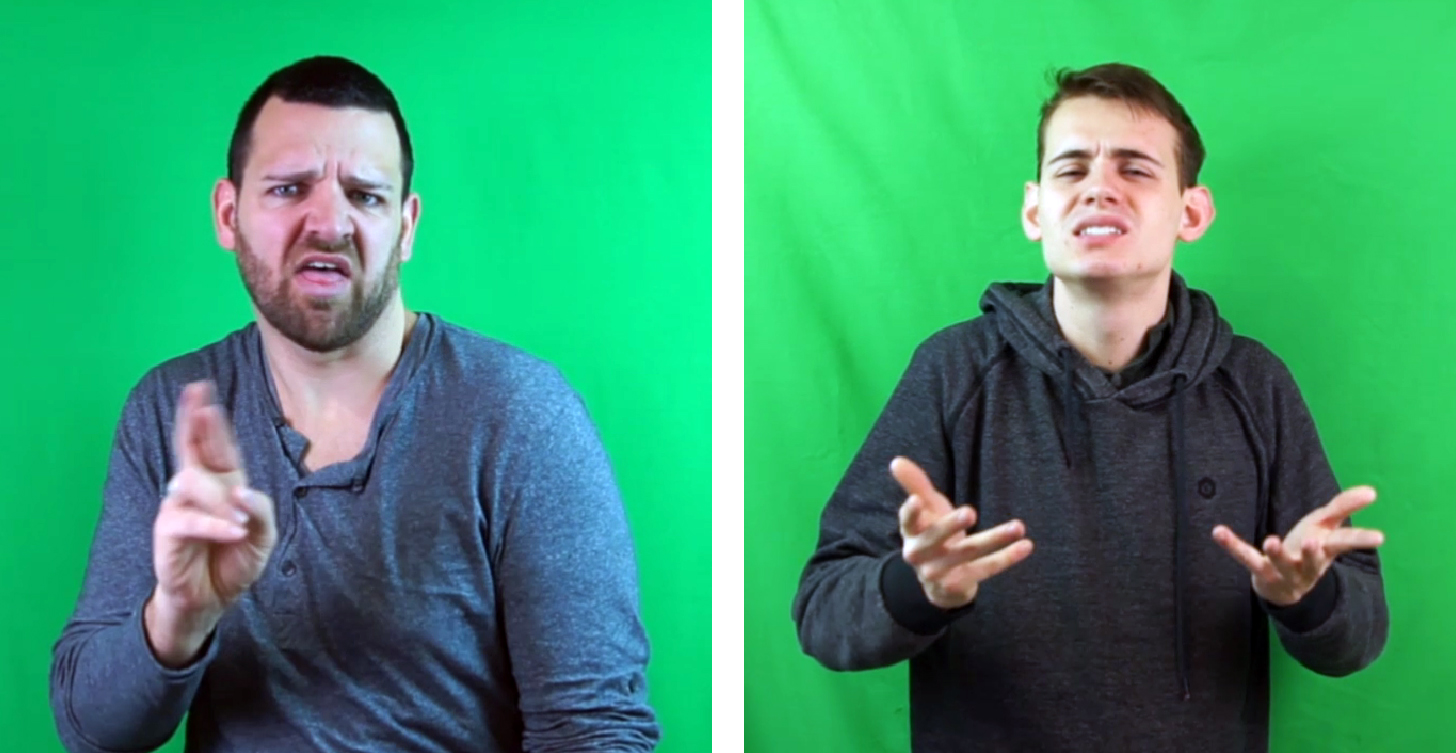
\includegraphics[width=1.0\textwidth]{nnmwhatwho.jpg}
	\caption{The non-manual markings used with constituent interrogatives in DGS consist of lowered brows and a squint. Additionally, the head is often put forwards towards the end of the clause. The signer on the left produces the sign \textsc{who}, the signer on the right the sign \textsc{what}.}
	\label{nnmwhatwho}
\end{figure}

As with polar interrogatives, the non-manuals used in \textit{wh}-questions have their intensity peak towards the end of the clause. This is true for the eyebrows and especially for moving the head forward, which mainly appears clause-finally. This is illustrated in Figure \ref{nnmwhatwhotwo}. The fact that the intensity peak is clause-final seems not to be influenced by the position of the \textit{wh}-phrase although in \textit{wh}-doubling, the clause-final \textit{wh}-phrase is typically focused. However, this seems not to be obligatory. Additionally, \textit{wh}-phrases may be focused in each position. 


\begin{figure}[bt]
\centering
	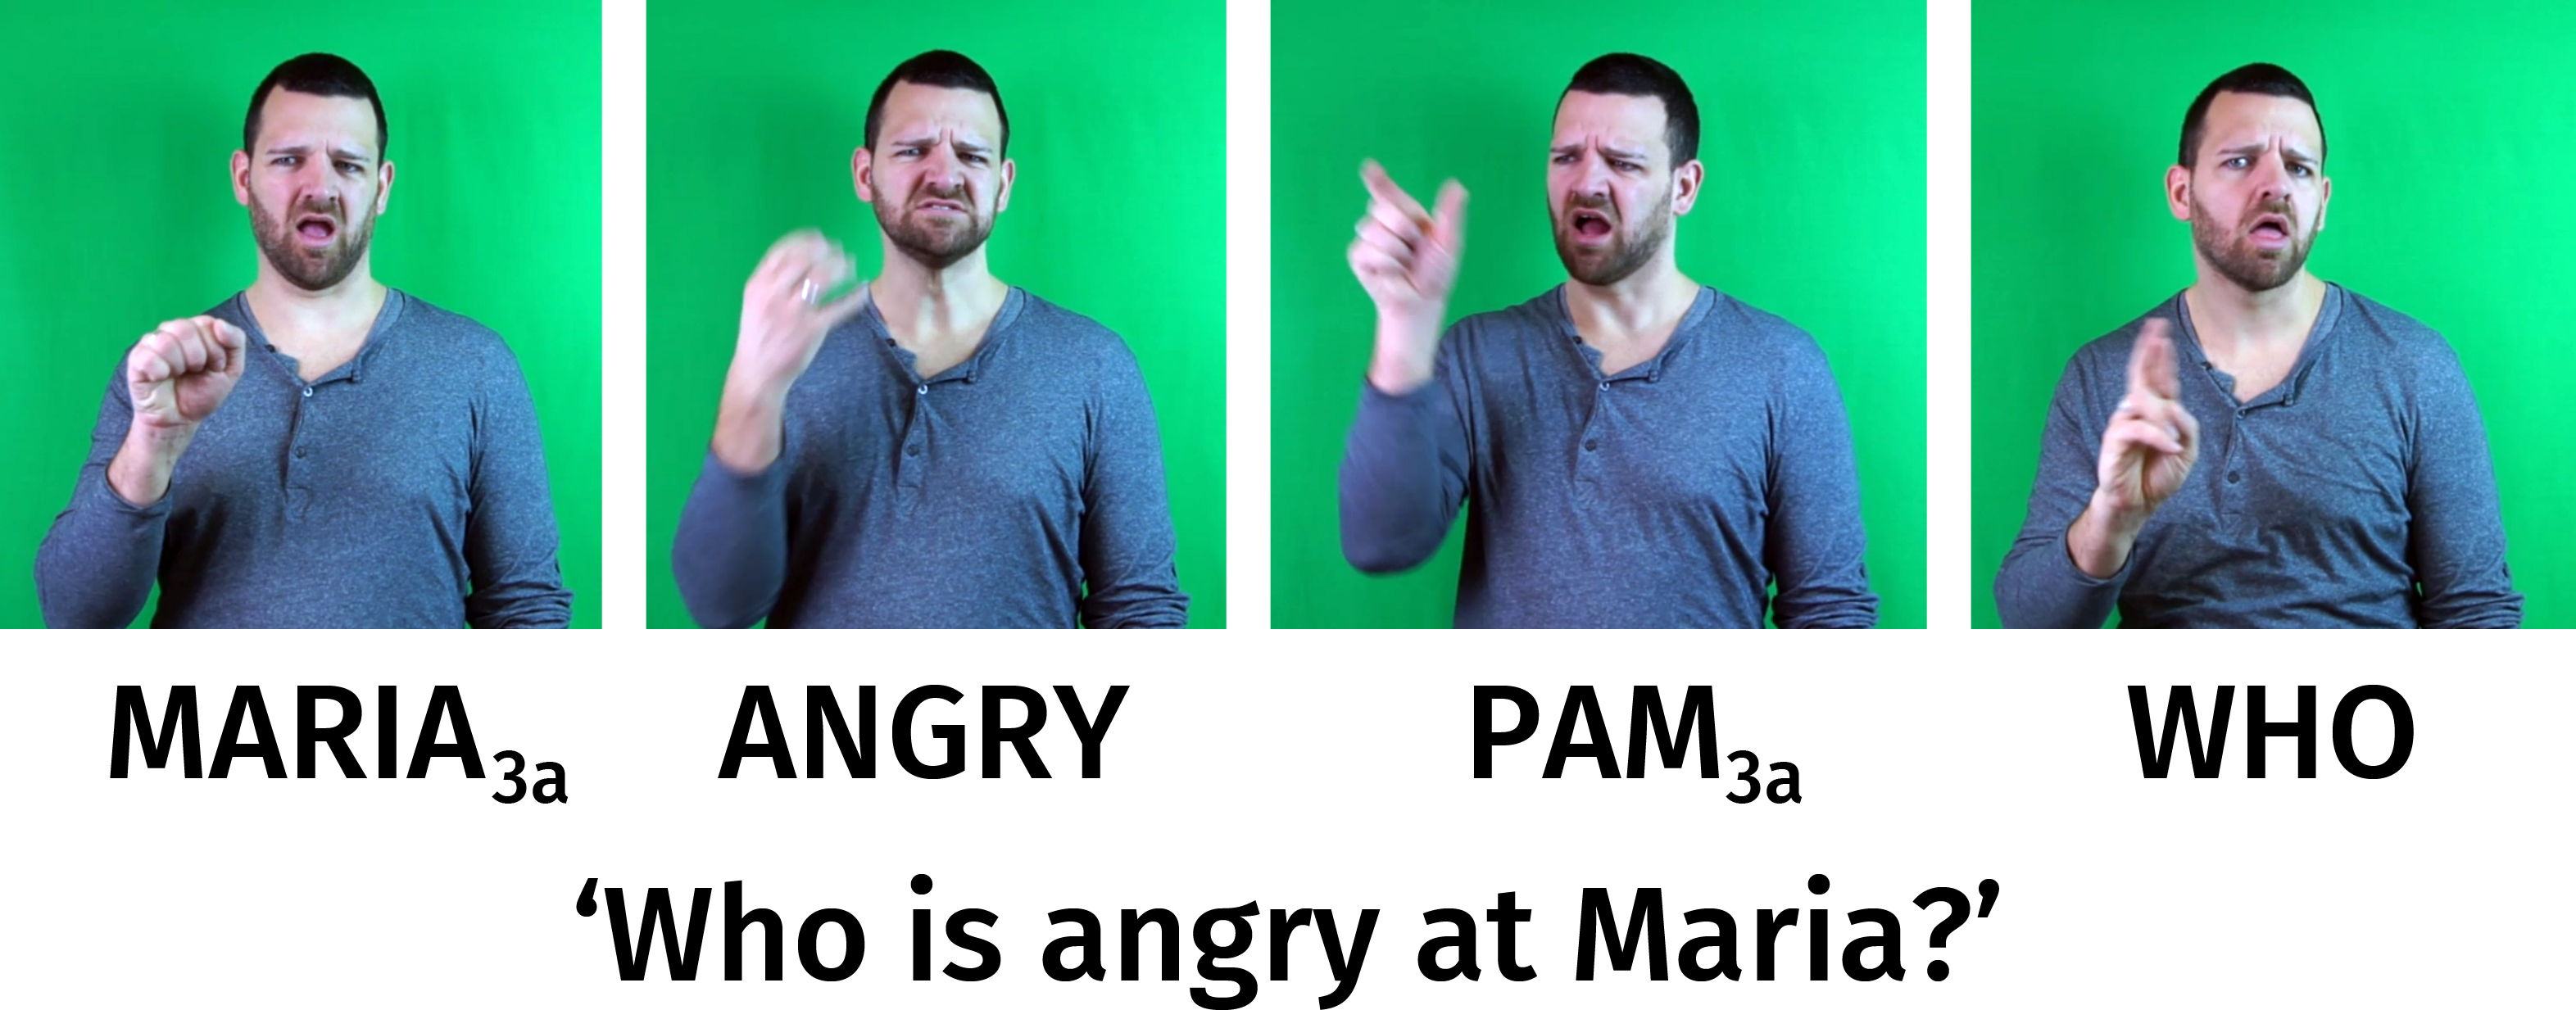
\includegraphics[width=1.0\textwidth]{whnonmanualsexample.jpg}
	\caption{The non-manual markings used with constituent interrogatives have their intensity peak clause-finally. As with polar interrogatives the head is put forward (as can be seen in the last picture).}
	\label{nnmwhatwhotwo}
\end{figure}

A last note concerns slight head-shakes that often accompany \textit{wh}-signs in DGS. This pattern was noted for other sign languages as well. \citet[232--235]{sarac2007cross}, for example, observed head shakes on \textit{wh}-signs in Croatian Sign Language. Similar to Croatian Sign Language, these head shakes in DGS only accompany the \textit{wh}-signs and do not spread further. Following \citet[235]{sarac2007cross}, I assume this head shake to be an ``assimilation with the movement of the hands'' as the hands often perform small repetitive movement with \textit{wh}-signs in DGS. Thus, I regard them to be a performance phenomenon and hence will not transcribe them.\footnote{ Although I do not want to exclude the possibility completely that there might be some semantic import from these slight head shakes.}

\subsubsection{\textit{Wh}-signs in DGS}


%WH Signs
DGS has a whole paradigm of \textit{wh}-signs including \textsc{who}, \textsc{what}, \textsc{how}, \textsc{why}, \textsc{how-so} (German gloss \textsc{wieso}), \textsc{when}, \textsc{how-much}, \textsc{which}, \textsc{where}, \textsc{from-where}, and \textsc{to-where}. Note that some signers sign \textsc{which} with a Y-handshape and some simply use the sign for \textsc{what}. Nevertheless, complex \textit{wh}-phrases of the sort \textit{which computer} syntactically behave in the same way regardless of which manual sign is used. Phonologically, most of the \textit{wh}-signs consist of small repetitive movements of one or two hands or the fingers. An additional sign that often surfaces in \textit{wh}-questions is the so called `palm-up' gesture (glossed \textsc{p-ug}) that was already discussed for polar interrogatives (see Section \ref{polarinterrogativesdgs}) consisting of all fingers spread out with the palm facing upwards (using one or both hands). 

\subsubsection{Positions of \textit{wh}-elements in DGS}
%Position of the wh-elements

The literature on DGS mainly reports clause-final and clause-initial \textit{wh}-signs, as well as doubling (e.\,g., \citealt{papaspyrou2008grammatik, happ2014vork}). My own data shows that \textit{in-situ} questions are also possible. One use of \textit{wh-in-situ} are echo questions. This is true for real echo questions in which a signer has understood what s/he is echoing as well as information-seeking echo questions.\footnote{ The difference between a real echo question and information-seeking echo questions is illustrated below -- note that it is unclear if the two types of echo questions actually behave differently in any language.

\begin{exe}
\ex\label{echoquestionillustrationenglish}\begin{xlist}
\ex A: Philip bought a new car.
\glt B: Philip bought a new \textsc{what}? He has no money to buy a new car! \label{echoquestionillustrationenglishb}
\ex A: Philip bought a new car.
\glt B: Philip bought a new \textsc{what}? I didn't understand you! \label{echoquestionillustrationenglisha}

\end{xlist}
\end{exe}

} However, I will leave echo questions aside in the following discussion.

A clause-structure theory of DGS dealing with constituent interrogatives should hence be able to explain -- at least -- the following possibilities. The unmarked position of \textit{wh}-phrases is the clause-final one, as in (\ref{ex:differentpositionsdgsa}). The example in (\ref{ex:differentpositionsdgsb}) shows that \textit{wh}-phrases can also occur clause-initially, although this is slightly marked as opposed to the clause-final pattern. The exact meaning differences between the clause-final and the clause-initial pattern have to be worked out. The third possibility that needs to be accounted for is doubling, shown in (\ref{ex:differentpositionsdgsaaaa}). 

\begin{exe}
\ex\label{differentpositionsdgs}
\begin{xlist} 
\ex \textcolor{white}{\%}\slg[wh]{yesterday beer buy who}
%
%\ex{} {\hspace{144pt}wh}  \\
%\textcolor{white}{\%}$\overline{\textrm{\textsc{yesterday beer buy who}}}$ 
\glt \textcolor{white}{\%}`Who bought beer yesterday?' \label{ex:differentpositionsdgsa} 
\ex \%\slg[wh]{who yesterday beer buy}
%
%\ex{} {\hspace{146pt}wh}  \\
%{\%$\overline{\textrm{\textsc{who yesterday beer buy}}}$} 
\glt \textcolor{white}{\%}`Who bought beer yesterday?' \label{ex:differentpositionsdgsb} 
\ex \textcolor{white}{\%}\slg[wh]{who yesterday beer buy who}
%
%\ex{} {\hspace{175pt}wh}  \\
%{} {\textcolor{white}{\%}$\overline{\textrm{\textsc{who yesterday beer buy who}}}$} 
\glt \textcolor{white}{\%}`Who bought beer yesterday?' \label{ex:differentpositionsdgsaaaa}
%\ex{} {\hspace{136pt}wh}  \\
%$\overline{\textrm{\textsc{yesterday who beer buy}}$}} 
%\glt `Who bought beer yesterday?' \label{ex:differentpositionsdgsc} 
\end{xlist}
\end{exe}

\noindent The fact that \textit{wh}-phrases can occur clause-finally, clause-initially, and can undergo doubling is in line with what was observed for other sign languages. Note that \textit{wh}-signs can receive focus regardless of position. However, when a \textit{wh}-sign is focused in a \textit{wh}-doubling construction it has to be the clause-final form that receives focus. In all cases, focus leads to a presuppositional reading. 

\begin{figure}[bt]
\centering
	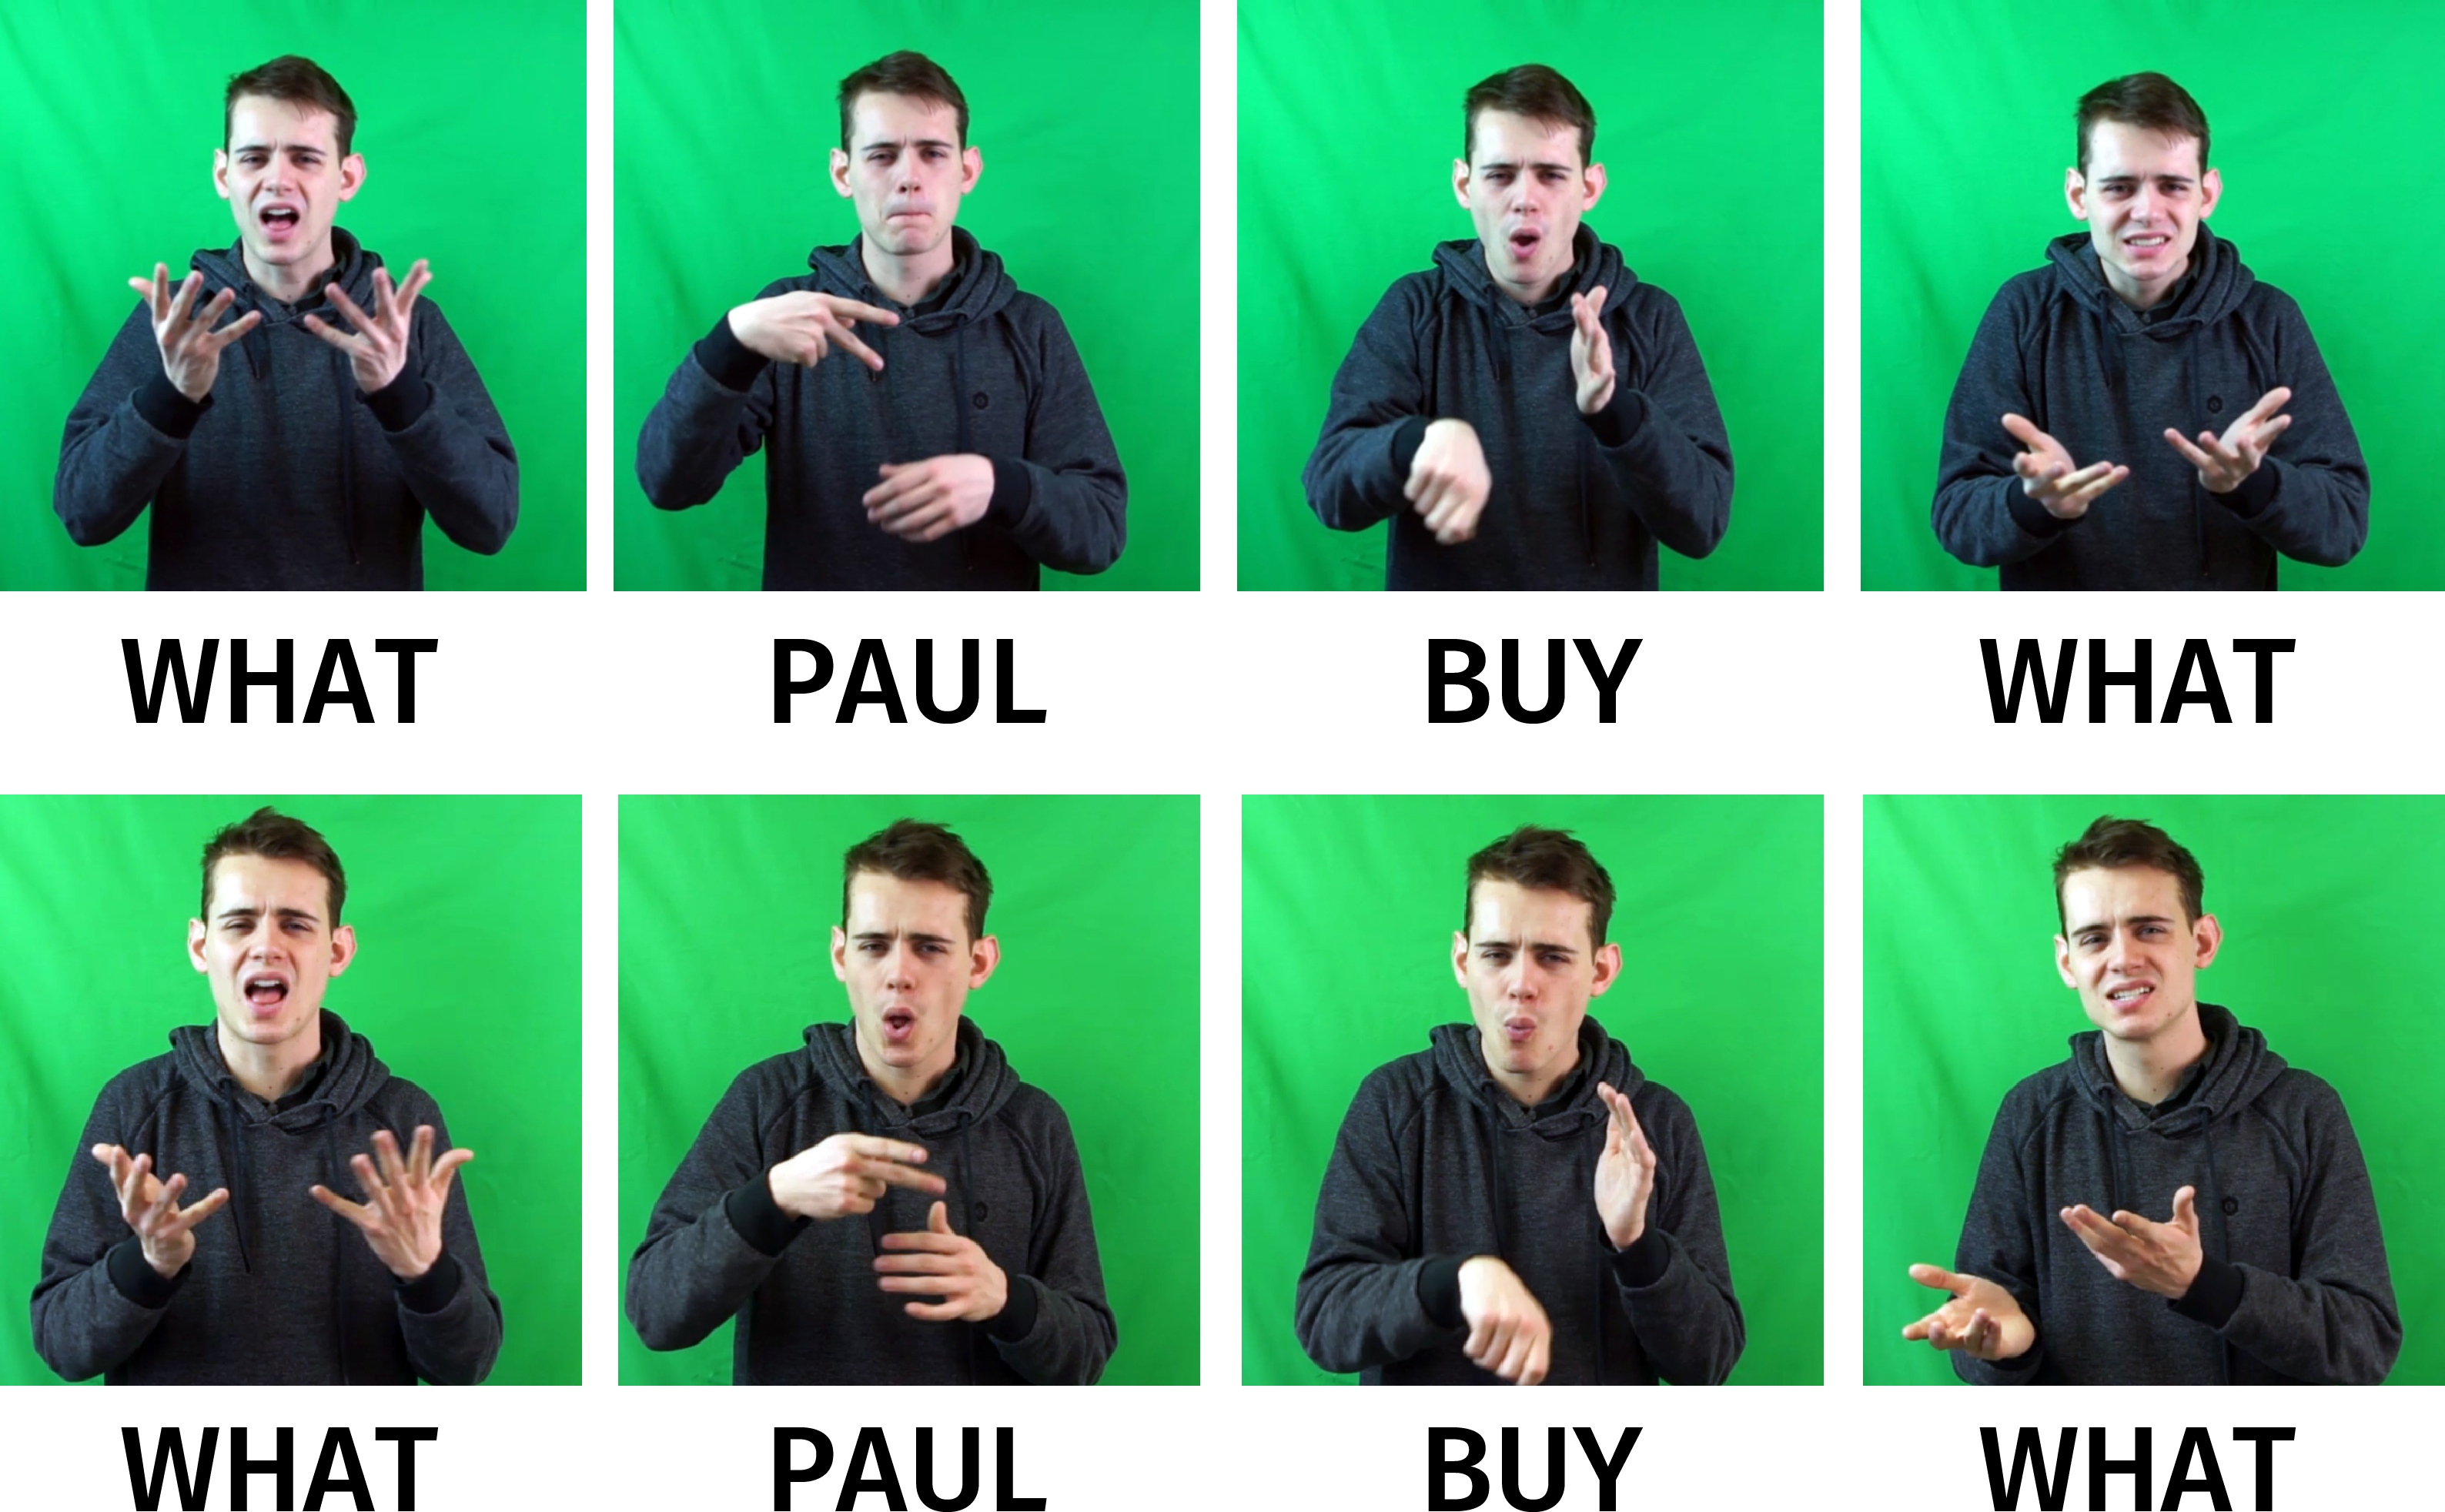
\includegraphics[width=1.0\textwidth]{whdoubling.jpg}
	\caption{With \textit{wh}-doubling two different patterns can be observed. In the first pattern, both \textit{wh}-signs are produced in neutral signing space. This is shown in the top example. In the second pattern, the first \textit{wh}-element is signed in neutral signing space (i.\,e., centered) while the second one is signed in a different position (on the side). This is shown in the bottom example. The examples show doubling in a sentence translating to \textit{What did Paul buy?}}
	\label{whdoubling}
\end{figure}

For \textit{wh}-doubling, two options are available. The first option consists of repeating the \textit{wh}-sign at the same location in signing space and for the second option, the clause-final sign is produced at a different location. Both types of \textit{wh}-doubling often receive an emphatic interpretation. Sentences in which the two instances are not produced in the same locations in signing space receive a (d-linked) set interpretation. Both cases are illustrated in Figure \ref{whdoubling}. The example at the bottom of the figure shows doubling with a set interpretation. This means that the signer indicates that it is clear to him that there is a set of items of which it is possible that Paul bought them and he wants to know which of this set Paul bought. The example at the top of the figure show doubling in the same location in signing space. 

Similar to what has been described for other sign languages, the picture that doubling presents in DGS is more complicated. As with American Sign Language, we find that doubling of complex \textit{wh}-phrases is not possible (\ref{ex:computerdoublinga}). Instead, it is possible to double only the simple \textit{wh}-phrase without its restrictor, as illustrated in (\ref{ex:computerdoublingb}). However, this pattern cannot be reversed, as in (\ref{ex:computerdoublingc}).

\vspace{0.5cm}

\begin{exe}
\ex\label{computerdoubling}
\begin{xlist} 
\ex *\slg[wh]{which computer paul buy which computer}
%
%\ex{} {\hspace{252pt}wh}  \\
%{} {*$\overline{\textrm{\textsc{which computer paul buy which computer}}}$} 
\glt \textcolor{white}{*}`Which computer did Paul buy?' \label{ex:computerdoublinga} 
\ex \textcolor{white}{*}\slg[wh]{which computer paul buy which}
%
%\ex{} {\hspace{188pt}wh}  \\
%{} {\textcolor{white}{*}$\overline{\textrm{\textsc{which computer paul buy which}}}$} 
\glt \textcolor{white}{*}`Which computer did Paul buy?' \label{ex:computerdoublingb} 
\ex *\slg[wh]{which paul buy which computer}
%
%\ex{} {\hspace{188pt}wh}  \\
%{} {*$\overline{\textrm{\textsc{which paul buy which computer}}}$} 
\glt \textcolor{white}{*}`Which computer did Paul buy?' \label{ex:computerdoublingc} 

\end{xlist}
\end{exe}

\noindent  Note that when no doubling is present, the \textit{wh}-phrase \textsc{which computer} is able to show up clause-initially or clause-finally. Interestingly, complex \textit{wh}-phrases show the exact opposite preferences as simple \textit{wh}-phrases. Thus, when no doubling is present, complex \textit{wh}-phrases systematically occur clause-initially, while the clause-final pattern, although well-formed, is the more marked version. This is shown in (\ref{computerdoublingonehundred}).

\begin{exe}
\ex\label{computerdoublingonehundred}
\begin{xlist} 
\ex \textcolor{white}{\%}\slg[wh]{which computer paul buy}
%
%\ex{} {\hspace{153pt}wh}  \\
%{} {\textcolor{white}{\%}$\overline{\textrm{\textsc{which computer paul buy}}}$} 
\glt \textcolor{white}{\%}`Which computer did Paul buy?' \label{ex:computerdoublingonehundreda} 
\ex \%\slg[wh]{paul buy which computer}
%
%\ex{} {\hspace{152pt}wh}  \\
%{} {\%$\overline{\textrm{\textsc{paul buy which computer}}}$} 
\glt \textcolor{white}{\%}`Which computer did Paul buy?' \label{ex:computerdoublingonehundreda} 
\end{xlist}
\end{exe}

\noindent Additionally, it is possible to move a \textit{wh}-element out of a complex \textit{wh}-phrase, as shown in (\ref{ex:splitexampledgs}). Thus, DGS shows what is traditionally called left-branch extraction \citep{bovskovic2005left, bovskovic2005locality}. Again, this extraction is only possible to the right, but not to the left (\ref{ex:splitexampledgsb}). However, the reason for sentence (\ref{ex:splitexampledgsb}) being ill-formed seems not to be due to syntactic reasons, but rather because of the fact that \textsc{which} and \textsc{paul} are adjacent which leads to the meaning \textit{which paul} which is not the desired meaning here.%\footnote{ My consultants did not like this construction exactly because of this reason. Note however, that *\textsc{which paul} itself is ill-formed as asking for a specific person is achieved by \textsc{person who}.}


\begin{exe}
\ex\label{blablablahunderttausend}\begin{xlist}
\ex \textcolor{white}{??}\slg[wh]{paul \textup{\textit{t}}_{\textup{i}} computer buy which_{\textup{i}}}
%
%\ex {\hspace{166pt}wh}  \\
%{\textcolor{white}{??}$\overline{\textrm{\textsc{paul} \textit{t}\textsubscript{i} \textsc{computer buy which}\textsubscript{i}}}$} 
\glt \textcolor{white}{??}`Which computer did Paul buy?' \label{ex:splitexampledgs}
\ex ??\slg[wh]{which_{\textup{i}} paul \textup{\textit{t}}_{\textup{i}} computer buy}
%
%\ex {\hspace{166pt}wh}  \\
%{??$\overline{\textrm{\textsc{which}\textsubscript{i} \textsc{paul} \textit{t}\textsubscript{i} \textsc{computer buy}}}$} 
\glt \textcolor{white}{??}`Which computer did Paul buy?' \label{ex:splitexampledgsb}
\end{xlist}
\end{exe} 

\noindent Similar extraction facts were described for spoken languages as well (see the following excursus).\label{leftbranchextractiona} Comparing the left-branch extraction in (\ref{ex:splitexampledgs}) with the partial doubling of complex \textit{wh}-phrases in (\ref{ex:computerdoublingb}) allows for different interpretations. Either one could call such structures partial doubling or interpret it as a complex clause-initial \textit{wh}-phrase plus left-branch extraction. Alternatively, the extracted \textsc{which} is an overt realization of operator movement that \citet{van2010complex} assumed to be empty in languages like English or German (see page \pageref{emptyoperator}). 

\begin{digression}{Left-branch extraction and determiners}{}
\noindent There is cross-linguistic variation as to the extraction of \textit{wh}-elements out of NP-/DP-internal constituents (see already \citealt{ross1967constraints}). This can be illustrated for complex \textit{wh}-phrases. While some languages do not allow movement of a \textit{wh}-element out of a complex constituent, others do allow this type of extraction, as illustrated in the English example in (\ref{leftbranchextractiona}) and the Serbo-Croatian example in (\ref{leftbranchextractionb}), both from \citet[14--15]{bovskovic2005left}. 



\begin{exe}
\ex\label{leftbranchextraction}\begin{xlist} 
\ex \textcolor{white}{*}English \\ *Whose\textsubscript{i} did you see $[$\textit{t}\textsubscript{i} father$]$? \label{leftbranchextractiona}
\ex \textcolor{white}{*}Serbo-Croatian \\ \gll {\textcolor{white}{*}\v{C}ijeg\textsubscript{i}} {si} {video} {$[$\textit{t}\textsubscript{i}} {oca$]$?}  \\
{\textcolor{white}{*}whose} {\textsc{clitic}} {seen} {} {father} \\
\trans \textcolor{white}{*}`Whose father did you see?' \label{leftbranchextractionb} 
\end{xlist}
\end{exe} 

\noindent The examples show that it is not possible for the \textit{wh}-word to move out of a \textit{wh}-phrase in English while this is allowed in Serbo-Croatian. \citet{bovskovic2005left, bovskovic2005locality} argues that the question of whether a language allows this so-called `left-branch extraction' or not is correlated with whether a language has overt determiners or not. In languages with overt determiners like English, so his argument, the DP forms a phase from which no extraction is allowed. In languages without overt determiners like Serbo-Croation, the DP does not form a phase and extraction is therefore allowed.

Like Serbo-Croation, DGS is a language lacking articles \citep[91]{happ2014vork} and similarly, DGS allows movement of a \textit{wh}-element out of a \textit{wh}-phrase as discussed above. Thus, DGS confirms \citeauthor{bovskovic2005left}'s (\citeyear{bovskovic2005left, bovskovic2005locality}) idea that languages without overt articles allow left-branch extraction.

Similar splits between a \textit{wh}-sign and its restriction were observed in other (articleless) sign languages as well. In Italian and Japanese Sign Language, for example, this is equally possible, as the example in (\ref{ex:splitexamplelisa}) from \citet[285]{cecchetto2009another} and the example in (\ref{ex:splitexamplelisb}) from \citet{fischer1998feature} cited in \citet[25]{zeshan2004interrogative} illustrate (\citealt{zeshan2004interrogative} also mentions that American Sign Language and Indo-Pakistani Sign Language allow for similar structures; for American Sign Language see also \citealt{boster1996quantifier}). 

\begin{exe}
\ex\label{splitexamplelis}\begin{xlist}
\ex Italian Sign Language \\\slg{boy book steal} \slg[wh]{which}
%\ex {} {\hspace{119pt}wh}  \\
%{\textsc{boy book steal}} {$\overline{\textrm{\textsc{which}}}$} 
\glt `Which boy stole the book?' \label{ex:splitexamplelisa} 
\ex Japanese Sign Language \\ \slg{color like} \slg[wh]{what}
%\ex {} {\hspace{85pt}wh}  \\
%{\textsc{color} \textsc{like} {$\overline{\textrm{\textsc{what}}}$}} 
\glt `Which color do you like?' \label{ex:splitexamplelisb} 
\end{xlist}
\end{exe} 

\noindent These examples show that in the case of left-branch extraction, articleless sign languages behave just as articleless spoken languages. 
\end{digression}


\noindent As with simple \textit{wh}-phrases (e.\,g., \textsc{what}) and in contrast to complex \textit{wh}-phrases (e.\,g., \textsc{which computer}), \textit{wh}-phrases contained in a PP may occur in a clause-final and -initial position as illustrated in (\ref{whphrasesinappdgs}), again with the clause-initial version being the slightly more marked one. Note that I analyze the signs \textsc{pam} and \textsc{bem} as being prepositions or preposition-like elements here (with \textsc{pam} meaning `at' and \textsc{bem} meaning `for'). See also the brief descriptions of the signs in the Section of notational conventions (on page \pageref{notational}).


%(note that the sign \textsc{pam}, an abbreviation for `person agreement marker' \citep{rathmann2003optionality}, is traditionally described as marking verb agreement)

%\hspace{-0.75cm}\begin{minipage}[t]{0.9\textwidth}
\begin{exe}
\ex\label{whphrasesinappdgs}
%\setlength{\columnsep}{1.5cm}
%\begin{multicols}{2}
\begin{xlist}
%$\overline{\textrm{}}$
\ex \textcolor{white}{\%}\slg[wh]{index_2 angry pam who}
%
%\ex {\hspace{129pt}wh}  \\
%{{\textcolor{white}{\%}$\overline{\textrm{\textsc{index}\textsubscript{2} \textsc{angry pam who}}}$}} 
\glt {\textcolor{white}{\%}`At whom are you angry?' \label{whphrasesinappdgsb}}
\ex \%\slg[wh]{pam who index_2 angry}
%
%\ex {\hspace{129pt}wh}  \\
%{\%$\overline{\textrm{\textsc{pam who index}\textsubscript{2} \textsc{angry}}}$} 
\glt {\textcolor{white}{\%}`At whom are you angry?' \label{whphrasesinappdgsa}}
\end{xlist}
%\end{multicols}
\end{exe}
%\end{minipage}


\noindent Crucially, phrases such as \textsc{which computer} are not syntactic operators as introduced in Section \ref{syntaxoperators} while simple \textit{wh}-phrases and \textit{wh}-phrases included in a PP are. This would predict that doubling of \textit{wh}-PPs should be acceptable in DGS. And indeed, doubling of a \textit{wh}-PP is possible, as illustrated in (\ref{doublingphrases}) and additionally in Figure \ref{whdoublinggg}. 

\begin{figure}[bt]
\centering
	\includegraphics[width=0.9\textwidth]{doubling.jpg}
	\caption{Examples of doubling of \textit{wh}-phrases contained in a PP.}
	\label{whdoublinggg}
\end{figure}

Note that I indicated that the examples are marked. In fact, signers judged the examples from being absolutely well-formed to being rather marked, but not ill-formed. This is in line with the observations on the doubling of PP-\textit{wh}-phrases in German (see page \pageref{whcopyinggermanb}) and in Northern Italian dialects (see page \pageref{morenorthernitalianab}). Also note that some, but not all signers reported that the acceptability improves with a short intonational break before the double, as indicated by the bracketed commas (similar to the Northern Italian examples).\footnote{ See \citet[324--325]{happ2014vork} for similar doubling examples discussed in different contexts. } 


\begin{exe}
\ex\label{doublingphrases}
\begin{xlist} 
\ex \%\slg[wh]{pam who index_2 angry(,) pam who}
%
%\ex{} {\hspace{199pt}wh}  \\
%{} {\%$\overline{\textrm{\textsc{pam who index}\textsubscript{2} \textsc{angry(,) pam who}}}$} 
\glt \textcolor{white}{\%}`At whom are you angry?' \label{ex:doublingphrasesa} 
\ex \%\slg[wh]{bem who index_2 cook(,) bem who}
%
%\ex{} {\hspace{195pt}wh}  \\
%{} {\%$\overline{\textrm{\textsc{bem who index}\textsubscript{2} \textsc{cook(,) bem who}}}$} 
\glt \textcolor{white}{\%}`For whom do you cook?' \label{ex:doublingphrasesb} 
\ex \%\slg[wh]{with who index_2 cook(,) with who}
%
%\ex{} {\hspace{206pt}wh}  \\
%{} {\%$\overline{\textrm{\textsc{with who index}\textsubscript{2} \textsc{cook(,) with who}}}$} 
\glt \textcolor{white}{\%}`With who do you cook?' \label{ex:doublingphrasesc} 
\end{xlist}
\end{exe}

\noindent Thus, with respect to the doubling of \textit{wh}-phrases contained in a PP, DGS patterns with Northern Italian dialects and with spoken German. 




\subsubsection{Analyzing the DGS data}

\noindent It is admittedly not easy to account for all the aforementioned facts in a syntactic model. For ease of understanding, I summarize the relevant facts that need to be accounted for in (\ref{overvieswhtypes}).

\begin{exe}
\ex\label{overvieswhtypes}
\begin{xlist}
\ex \textcolor{white}{\%}\textit{Clause-final simple \textit{wh}-phrase:}\\
\textcolor{white}{\%}\slg[wh]{today \textup{\textit{t}}_{\textup{i}} beer buy who_{\textup{i}}}
\label{overvieswhtypesa}
\ex \textcolor{white}{\%}\textit{Clause-initial simple \textit{wh}-phrase (slightly marked):}\\
\%\slg[wh]{who_{\textup{i}} (today) \textup{\textit{t}}_{\textup{i}} beer buy}
\label{overvieswhtypesb}
\ex \textcolor{white}{\%}\textit{Doubling of a simple \textit{wh}-phrase:}\\
\textcolor{white}{\%}\slg[wh]{who_{\textup{i}} (today) \textup{\textit{t}}_{\textup{i}} beer buy who}
\label{overvieswhtypesc}
\ex \textcolor{white}{\%}\textit{Clause-initial complex \textit{wh}-phrase:}\\
\textcolor{white}{\%}\slg[wh]{[which car]_{\textup{i}} paul \textup{\textit{t}}_{\textup{i}} buy}
\label{overvieswhtypesd}
\ex \textcolor{white}{\%}\textit{Left-branch extraction to the right:}\\
\textcolor{white}{\%}\slg[wh]{paul \textup{\textit{t}}_{\textup{i}} car buy which_{\textup{i}}}
\label{overvieswhtypese}
\ex \textcolor{white}{\%}\textit{Illicit left-branch extraction to the left:}\\
??\slg[wh]{which_{\textup{i}} paul \textup{\textit{t}}_{\textup{i}} car buy}
\label{overvieswhtypesf}
\ex \textcolor{white}{\%}\textit{Clause-final complex \textit{wh}-phrase (slightly marked):}\\
\textcolor{white}{*}\%\slg[wh]{paul \textup{\textit{t}}_{\textup{i}} buy [which car]_{\textup{i}}}
\label{overvieswhtypesg}
\ex \textcolor{white}{*\%}\textit{Illicit complex doubling:} \\
\textcolor{white}{\%}*\slg[wh]{[which car]_{\textup{i}} paul \textup{\textit{t}}_{\textup{i}} buy [which car]_{\textup{i}}}
\label{overvieswhtypesh}
\ex \textcolor{white}{*\%}\textit{Initial complex \textit{wh} $+$ extraction:} \\
\textcolor{white}{*\%}\slg[wh]{[which car]_{\textup{i}} paul \textup{\textit{t}}_{\textup{i}} buy which_{\textup{i}}}
\label{overvieswhtypesi}
\ex \textcolor{white}{*\%}\textit{Final complex \textit{wh} $+$ extraction:} \\
\textcolor{white}{\%}*\slg[wh]{which_{\textup{i}} paul \textup{\textit{t}}_{\textup{i}} buy [which car]_{\textup{i}}}
\label{overvieswhtypesj}

\end{xlist}

\end{exe}

\noindent The examples from (\ref{overvieswhtypesa}) to (\ref{overvieswhtypesc}) are, as discussed, the ones that could also contain a \textit{wh}-phrase contained in a PP (e.\,g., \textsc{with who}). Thus, it is clear that we need to provide two specifier positions. The bracketed temporal adverbs indicate the clause-initial position in declarative sentences. The structure in (\ref{overvieswhtypesd}) is the neutral way to ask a question containing a complex \textit{wh}-phrase, (\ref{overvieswhtypese}) shows a left-branch extraction, (\ref{overvieswhtypesf}) the illicit left-branch extraction. The example in (\ref{overvieswhtypesg}) shows a slightly marked, but grammatical construction with a clause-final complex \textit{wh}-phrase. In (\ref{overvieswhtypesh}), the illicit doubling of a complex \textit{wh}-phrase is illustrated and (\ref{overvieswhtypesi}) shows the possible doubling. Finally, (\ref{overvieswhtypesj}) shows that the opposite option with an extracted simple \textit{wh}-element clause-initially and a clause-final complex \textit{wh}-phrase is not a licit structure in DGS.


In the following I will propose two different models to account for the data in (\ref{overvieswhtypes}). The first model will follow the rightward-movement tradition and the second model will follow the Kayneian idea that the order specifier--head--complement is fixed (thus, all heads will be left-headed and all specifiers will also be to the left). Both accounts will need to make use of remnant movement.
\vspace{-0.3cm}
\subsubsection{Syntactic analyses: two possiblities}
\vspace{-0.3cm}
If we follow the van Craenenbroek model, we would assume that CP\textsubscript{1}, but not CP\textsubscript{2} is a possible host for complex \textit{wh}-phrases. Similar to Strijen Dutch (see page \pageref{vancraenenbroekdutchdialecta}), the general landing site for simple \textit{wh}-phrases and \textit{wh}-phrases contained in a PP is CP\textsubscript{2}. These assumptions will hold for both models.

I will first show how to implement this in a mixed-branching structure. SpecCP\textsubscript{2} is right-branching in this model, as \textit{wh}-phrases obviously occur to the right in DGS. In contrast to simple \textit{wh}-phrases and \textit{wh}-phrases contained in a PP, complex \textit{wh}-phrases cannot be hosted in CP\textsubscript{2} (again similar to Strijen Dutch), but are base-generated in CP\textsubscript{1}, that I take to be the mirror image of CP\textsubscript{2}, i.\,e., left-branching (note that I simply posit that the heads are on the same side as the specifiers in the following). 

A simple constituent interrogative like \textsc{beer buy who} is then derived by moving the \textit{wh}-phrase \textsc{who} to SpecCP\textsubscript{2}, as shown in (\ref{ex:firstanalysisababaa}). A clause-initial constituent interrogative like \textsc{who beer buy} is derived by first moving the \textit{wh}-phrase \textsc{who} to SpecCP\textsubscript{2} and from there, in a cyclic fashion, to SpecCP\textsubscript{1}. In this case, the intermediate copy of \textsc{who} (in SpecCP\textsubscript{2}) is deleted. Additionally, it is possible to spell out this copy resulting in a doubling construction (\textsc{who beer buy who}). These options are shown in (\ref{ex:firstanalysisababab}). The optional deletion of the copy in SpecCP\textsubscript{2} is indicated by the gray color of the \textit{wh}-phrase.
\clearpage
\begin{exe}
\ex\label{ex:firstanalysisababa}
\begin{multicols}{2}
\begin{xlist}
\ex \label{ex:firstanalysisababaa}
\begin{adjustbox}{max width=0.38\textwidth}
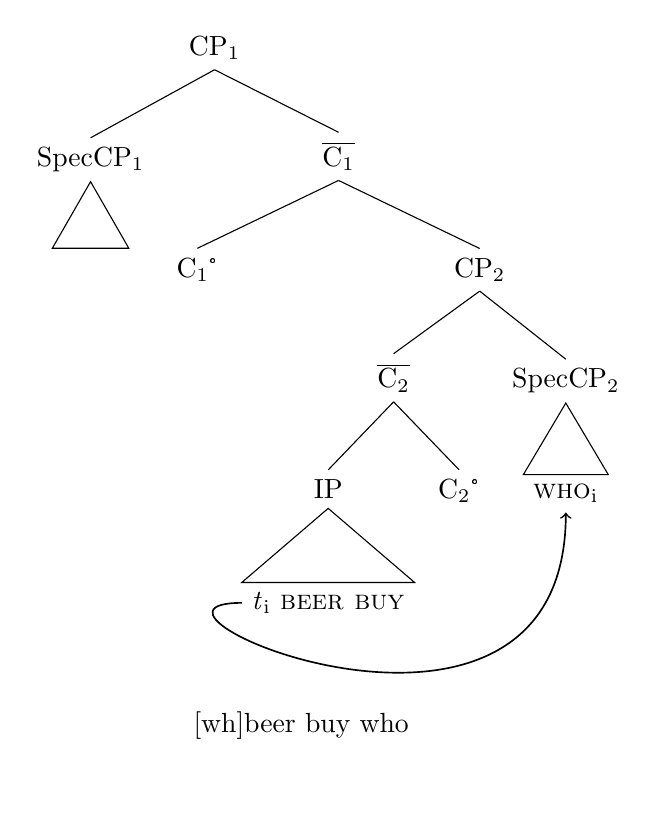
\begin{tikzpicture}[baseline]
\tikzset{level distance=40pt,sibling distance=5pt}
\Tree [.{CP\textsubscript{1}} [.SpecCP\textsubscript{1} \edge[roof]; \node(cp1){\textcolor{white}{who\textsubscript{i}}}; ] [.{$\overline{\textrm{C\textsubscript{1}}}$} [.{C\textsubscript{1}\textdegree} ] [.{CP\textsubscript{2}} [.{$\overline{\textrm{C\textsubscript{2}}}$} [.IP \edge[roof]; \node(ip){$\textrm{\textit{t}}$\textsubscript{i} \textsc{beer buy}}; ] [.{C\textsubscript{2}\textdegree} ] ] [.SpecCP\textsubscript{2} \edge[roof]; \node(cp2){\textsc{who}\textsubscript{i}}; ] ] ] ]
\draw[semithick,->] (ip)..controls +(west:3) and +(south:4)..(cp2);
\node (text) at (1.10,-8.5) {\slg[wh]{beer buy who}};
%\node (overlinetext) at (2.3,-8.1) {wh};
%\node (text) at (1.10,-8.5) {$\overline{\textrm{\textsc{beer buy who}}}$};
\end{tikzpicture}
\end{adjustbox}
\ex\label{ex:firstanalysisababab}
\begin{adjustbox}{max width=0.38\textwidth}
\begin{tikzpicture}[baseline]
\tikzset{level distance=40pt,sibling distance=5pt}
\Tree [.{CP\textsubscript{1}} [.SpecCP\textsubscript{1} \edge[roof]; \node(cp1){\textsc{who}\textsubscript{i}}; ] [.{$\overline{\textrm{C\textsubscript{1}}}$} [.{C\textsubscript{1}\textdegree} ] [.{CP\textsubscript{2}} [.{$\overline{\textrm{C\textsubscript{2}}}$} [.IP \edge[roof]; \node(ip){$\textrm{\textit{t}}$\textsubscript{i} \textsc{beer buy}}; ] [.{C\textsubscript{2}\textdegree} ] ] [.SpecCP\textsubscript{2} \edge[roof]; \node(cp2){\textcolor{gray}{\textsc{who}\textsubscript{i}}}; ] ] ] ]
%\draw[semithick, <-] (cp2.south) to [bend right=-60] (ip.base west);
\draw[semithick,->] (ip)..controls +(west:3) and +(south:4)..(cp2);
\draw[semithick,->] (cp2)..controls +(south east:3) and +(south:10)..(cp1);
\node (text) at (1.8,-9.7) {\slg[wh]{who beer buy (who)}};

%\node (overlinetext) at (3.72,-9.22) {wh};
%\node (text) at (1.8,-9.7) {$\overline{\textrm{\textsc{who beer buy (who)}}}$};

\end{tikzpicture}
\end{adjustbox}
\end{xlist}
\end{multicols}
\end{exe}

\noindent One advantage of this modeling possibility is that the more marked case, namely sentences containing a clause-initial simple \textit{wh}-phrase, needs an additional movement step (as well as the doubling construction which is generally more marked than a \textit{wh}-question with only one \textit{wh}-phrase). 

The next step is to account for complex \textit{wh}-phrases like \textsc{which computer}. Under the assumption that complex \textit{wh}-phrases are base-generated in SpecCP\textsubscript{1}, we simply get the structure in (\ref{ex:firstanalysisaba}). Following van Craenenbroek's ideas completely, one could assume empty operator movement in this case too. Additionally, it is possible to account for left-branch extraction, as shown in (\ref{ex:firstanalysisabb}). This case could be seen as an overt manifestation of the empty operator movement. Combining the two mechanisms results in the partial doubling found with complex \textit{wh}-phrases (e.\,g., \textsc{which computer paul buy which}). %Thus, the empty operator movement van Craenenbroek (2010) assumed, is visible in DGS.

The structures in (\ref{ex:firstanalysisab}) also account for the ill-formedness of doubling in cases of complex \textit{wh}-phrases, as there is only one possible host for this type of \textit{wh}-phrase, namely SpecCP\textsubscript{1}. Left-branch extraction to the left, however, should be possible in principle. And indeed, it is (this would probably be cyclical as well). However, extracting the operator to the left makes it adjacent to the first sign in the sentence that, in this case, leads to the odd reading `Which Paul is buying a computer?' 

\begin{exe}
\ex\label{ex:firstanalysisab}
\begin{multicols}{2}
\begin{xlist}
\ex \label{ex:firstanalysisaba}
\begin{adjustbox}{max width=0.45\textwidth}
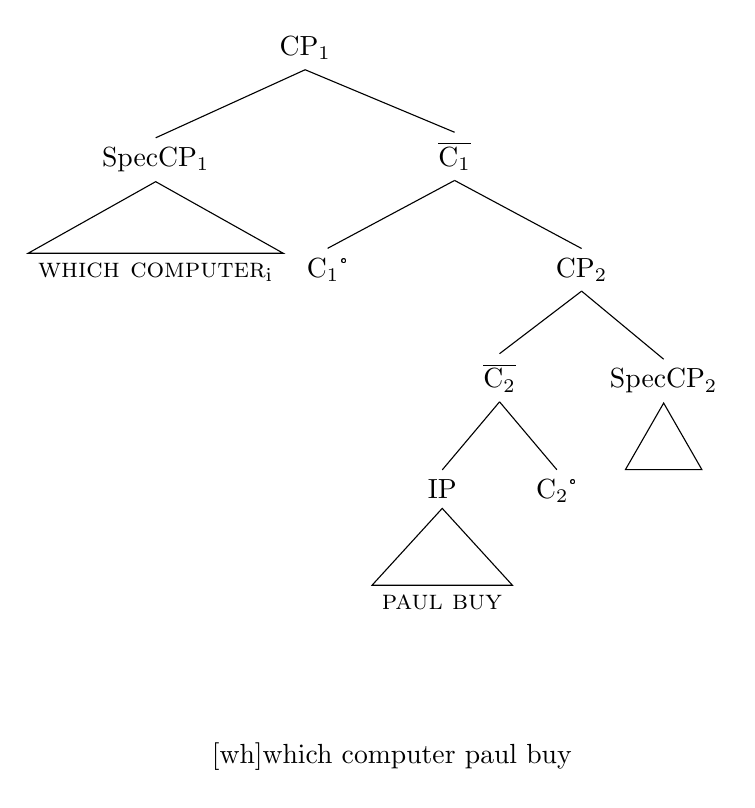
\begin{tikzpicture}[baseline]
\tikzset{level distance=40pt,sibling distance=5pt}
\Tree [.{CP\textsubscript{1}} [.SpecCP\textsubscript{1} \edge[roof]; \node(cp1){\textsc{which computer}\textsubscript{i}}; ] [.{$\overline{\textrm{C\textsubscript{1}}}$} [.{C\textsubscript{1}\textdegree} ] [.{CP\textsubscript{2}} [.{$\overline{\textrm{C\textsubscript{2}}}$} [.IP \edge[roof]; \node(ip){\textsc{paul} \textsc{buy}}; ] [.{C\textsubscript{2}\textdegree} ] ] [.SpecCP\textsubscript{2} \edge[roof]; \node(cp2){\textcolor{white}{who\textsubscript{i}}}; ] ] ] ]
\node (text) at (1.10,-8.9) {\slg[wh]{which computer paul buy}};
%\draw[semithick,->] (ip)..controls +(south:3) and +(south:4)..(cp1);
%\draw[semithick, <-] (cp2.south) to [bend right=-60] (ip.base west);
%\node (overlinetext) at (3.65,-8.5) {wh};
%\node (text) at (1.10,-8.9) {$\overline{\textrm{\textsc{which computer} \textsc{paul} \textsc{buy}}}$};
\end{tikzpicture}
\end{adjustbox}
\ex\label{ex:firstanalysisabb}
\begin{adjustbox}{max width=0.45\textwidth}
\begin{tikzpicture}[baseline]
\tikzset{level distance=40pt,sibling distance=2.5pt}
\Tree [.{CP\textsubscript{1}} [.SpecCP\textsubscript{1} \edge[roof]; \node(cp1){\textcolor{white}{\textsc{computer}\textsubscript{i}}}; ] [.{$\overline{\textrm{C\textsubscript{1}}}$} [.{C\textsubscript{1}\textdegree} ] [.{CP\textsubscript{2}} [.{$\overline{\textrm{C\textsubscript{2}}}$} [.IP \edge[roof]; \node(ip){\qquad\textsc{paul} $\textrm{\textit{t}}$\textsubscript{i} \textsc{computer buy}\qquad}; ] [.{C\textsubscript{2}\textdegree} ] ] [.SpecCP\textsubscript{2} \edge[roof]; \node(cp2){\textsc{which}\textsubscript{i}}; ] ] ] ]
\draw[semithick,->] (ip)..controls +(south west:0.1) and +(south:4)..(cp2);
%\draw[semithick, <-] (cp2.south) to [bend right=-60] (ip.base west);
\node (text) at (1.8,-10.3) {\slg[wh]{paul \textup{\textit{t}}_{\textup{i}} computer buy which_{\textup{i}}}};

%\node (overlinetext) at (4.55,-9.8) {wh};
%\node (text) at (1.8,-10.3) {$\overline{\textrm{\textsc{paul} $t$\textsubscript{i} \textsc{computer buy which}\textsubscript{i}}}$};
\end{tikzpicture}
\end{adjustbox}
\end{xlist}
\end{multicols}
\end{exe}

The last thing to model is a clause-final complex \textit{wh}-phrase. For this, an additional remnant movement needs to be assumed. The tree in (\ref{remnantmovementoftheipwithtwocps}) shows how this could be implemented in the current model. It is, however, unclear into which position this movement would be, but one could assume that it is SpecForceP. 

\begin{exe}
\ex\label{remnantmovementoftheipwithtwocps}
\begin{adjustbox}{max width=0.80\textwidth}
\begin{tikzpicture}[baseline]
\tikzset{level distance=40pt,sibling distance=10pt}
\Tree [.ForceP [.SpecForceP \edge[roof]; \node(sleepyman){\textcolor{white}{something here}}; ] [.{$\overline{\textrm{Force}}$} [.{Force\textdegree} ] [.{CP\textsubscript{1}} [.SpecCP\textsubscript{1} \edge[roof]; \node(cp1){\textsc{which computer}\textsubscript{i}}; ] [.{$\overline{\textrm{C\textsubscript{1}}}$} [.{C\textsubscript{1}\textdegree} ] [.{CP\textsubscript{2}} [.{$\overline{\textrm{C\textsubscript{2}}}$} [.IP \edge[roof]; \node(ip){\textsc{paul} \textcolor{white}{$\textrm{\textit{t}}$\textsubscript{i}} \textsc{buy}}; ] [.{C\textsubscript{2}\textdegree} ] ] [.SpecCP\textsubscript{2} \edge[roof]; \node(cp2){\textcolor{white}{\textsc{which}\textsubscript{i}}}; ] ] ] ] ] ] 

%\draw[semithick,->] (ip)..controls +(south:2) and +(south:4)..(cp1);
%\draw[semithick, <-] (cp2.south) to [bend right=-60] (ip.base west);

\node (A) at (8.7,-11.0) {};
%\draw[semithick,->] (A)..controls +(south:3) and +(south:4)..(sleepyman);
%\draw[semithick,->] (ip.south) to [bend right=-80] node [midway,fill=white] {Step 1} (cp1.south);
%\draw[semithick,->] (A)..controls +(south west:0.1) and +(south:4)..(sleepyman);
\draw[semithick,->] (A.south) to [bend right=-80] (sleepyman.south);
\draw[gray] (8.3,-7.1) circle (4cm);

\end{tikzpicture}
\end{adjustbox}
\end{exe}

\vspace{-0.8cm}

\noindent The additional remnant movement is not that farfetched as the resulting structure is more marked than the clause-initial one. Thus, again, a marked structure is derived by an additional movement step.

One open point is the spreading behavior of the non-manuals. Considering the insights gained about polar interrogatives from the previous section, we could say that the IntP is located above the \textit{wh}-landing sites. The spreading of the non-manuals can, again, be assumed to be regulated by Int\textdegree\ which should be right-headed to account for the non-manuals being strongest clause-finally. This is indeed the case. Additionally, \textit{wh}-question in DGS can always be followed by \textsc{p-ug}. This sign was also described for constituent interrogatives in other sign languages. Notably, \citet{aboh2010sa} analyze the clause-final palm-up gesture in \textit{wh}-questions in the Sign Language of the Netherlands as an instantiation of Inter\textdegree . In Sign Language of the Netherlands and in DGS, the palm-up gesture is found in the very last position of the clause. Compare the data from \citet[111]{aboh2010sa} in (\ref{ex:abohpfaupug}) and the DGS examples in (\ref{pugdgs}).

\begin{exe}
\ex Sign Language of the Netherlands \citep[111]{aboh2010sa} \\ \slg[wh]{poss_2 bike steal who p-ug}
\glt `Who stole your bike?' \label{ex:abohpfaupug} 
\end{exe}

\begin{exe}
\ex\label{pugdgs}
\begin{xlist} 
\ex \slg[wh]{maria angry pam who p-ug}
%\ex {\hspace{148pt}wh}  \\
%$\overline{\textrm{\textsc{maria angry pam who p-ug}}}$ 
\glt `At whom is Maria angry?' \label{ex:pugdgsa} 
\ex \slg[wh]{who pam maria angry p-ug}
%\ex {\hspace{148pt}wh}  \\
%$\overline{\textrm{\textsc{who pam maria angry p-ug}}}$
\glt `Who is angry at Maria?' \label{ex:pugdgsb} 
\end{xlist}
\end{exe}

\noindent Thus, if \textsc{p-ug} is indeed located in Inter\textdegree\ and if this head is also triggering the non-manuals in constituent interrogatives, the proposed model is completely in line with the data. Assuming that the non-manuals are triggered by Inter\textdegree\ in both, polar and constituent questions, however, poses the question why the non-manuals in polar and constituent questions differs in DGS. I will leave this open for further research.   %Especially, when taking into account that focused \textit{wh}-signs in doubling constructions are also accompanied by 

Alternatively, a similar idea would be to model \textit{wh}-movement in DGS similar to what was proposed for Northern Italian earlier (cf. page \pageref{italianwhdoublinga}), i.\,e., with an additional projection between CP\textsubscript{1} and CP\textsubscript{2}. While this model clearly is more elegant, as it is possible to construct it in a more Kayneian way (with all specifiers and heads to the left) it has the disadvantage of requiring a lot more (remnant) movement steps that are hard to motivate and an additional projection. The overall model would have the structure in (\ref{remnantmovementitalianstyle}).%If one tries to motivate this remnant movement along similar lines as Aboh \& Pfau (2010), namely by assuming that there is a strong Int\textdegree\ that attracts the remnant into it's specifier, the structure would in general look like the following. 

In this model, it has to be assumed that after all movement steps are completed, the remainder of the clause is moved into the specifier of the InterP. Assuming that it is feature checking between SpecInterP and Inter\textdegree\ that triggers the non-manual markings, all material is accompanied by brow lowering with the intensity peak being clause-final. 

\vspace{-0.3cm}

\begin{exe}
\ex\label{remnantmovementitalianstyle}
\begin{adjustbox}{max width=0.90\textwidth}
\begin{tikzpicture}[baseline]
\tikzset{level distance=30pt,sibling distance=10pt}
\Tree [.{InterP} [.SpecInterP \edge[roof]; \node(specintp){\textcolor{white}{something here}}; ] [.{$\overline{\textrm{Int}}$} [.{Inter\textdegree } ] [.{CP\textsubscript{1}} [.SpecCP\textsubscript{1} \edge[roof]; \node(speccp1){\textcolor{white}{something here}}; ] [.{$\overline{\textrm{CP\textsubscript{1}}}$} [.{C\textsubscript{1}\textdegree} ] [.{XP} [.SpecXP \edge[roof]; \node(specintp){\textcolor{white}{something here}}; ] [.{$\overline{\textrm{X}}$} [.{X\textdegree } ] [.{CP\textsubscript{2}} [.SpecCP\textsubscript{2} \edge[roof]; \node(speccp2){\textcolor{white}{something here}}; ] [.{$\overline{\textrm{CP\textsubscript{2}}}$} [.{C\textsubscript{1}\textdegree} ] [.IP \edge[roof]; \node(ip){\textcolor{white}{something here}}; ] ] ] ] ] ] ] ] ]

%[.IP \edge[roof]; \node(ip){\textsc{paul} $t$\textsubscript{i} \textsc{buy}}; ]


\end{tikzpicture}
\end{adjustbox}
\end{exe}


\vspace{-0.3cm}


\noindent I will start again with clause-final simple \textit{wh}-phrases -- ignoring the fact that, in the end, all remaining material moves to SpecInter for the moment. First, the \textit{wh}-phrase is moved into SpecCP\textsubscript{2} and then, the rest of the clause is moved into SpecXP. This is shown in (\ref{ex:firstanalysisatwoa}). Clause-initial simple \textit{wh}-phrases are modeled by one additional step, namely by moving the \textit{wh}-phrase into the specifier of SpecCP\textsubscript{1}. This option is shown in (\ref{ex:firstanalysisbtwob}). Again, the more marked structure (the clause-initial simple \textit{wh}-phrase) is derived by additional movement and doubling is, again, achieved by not deleting the copy that is created in the first movement step.

\vspace{-0.5cm}


\begin{exe}
\ex\label{ex:firstanalysistwo}
\begin{multicols}{2}
\begin{xlist}
\ex \label{ex:firstanalysisatwoa}
\begin{adjustbox}{max width=0.46\textwidth}
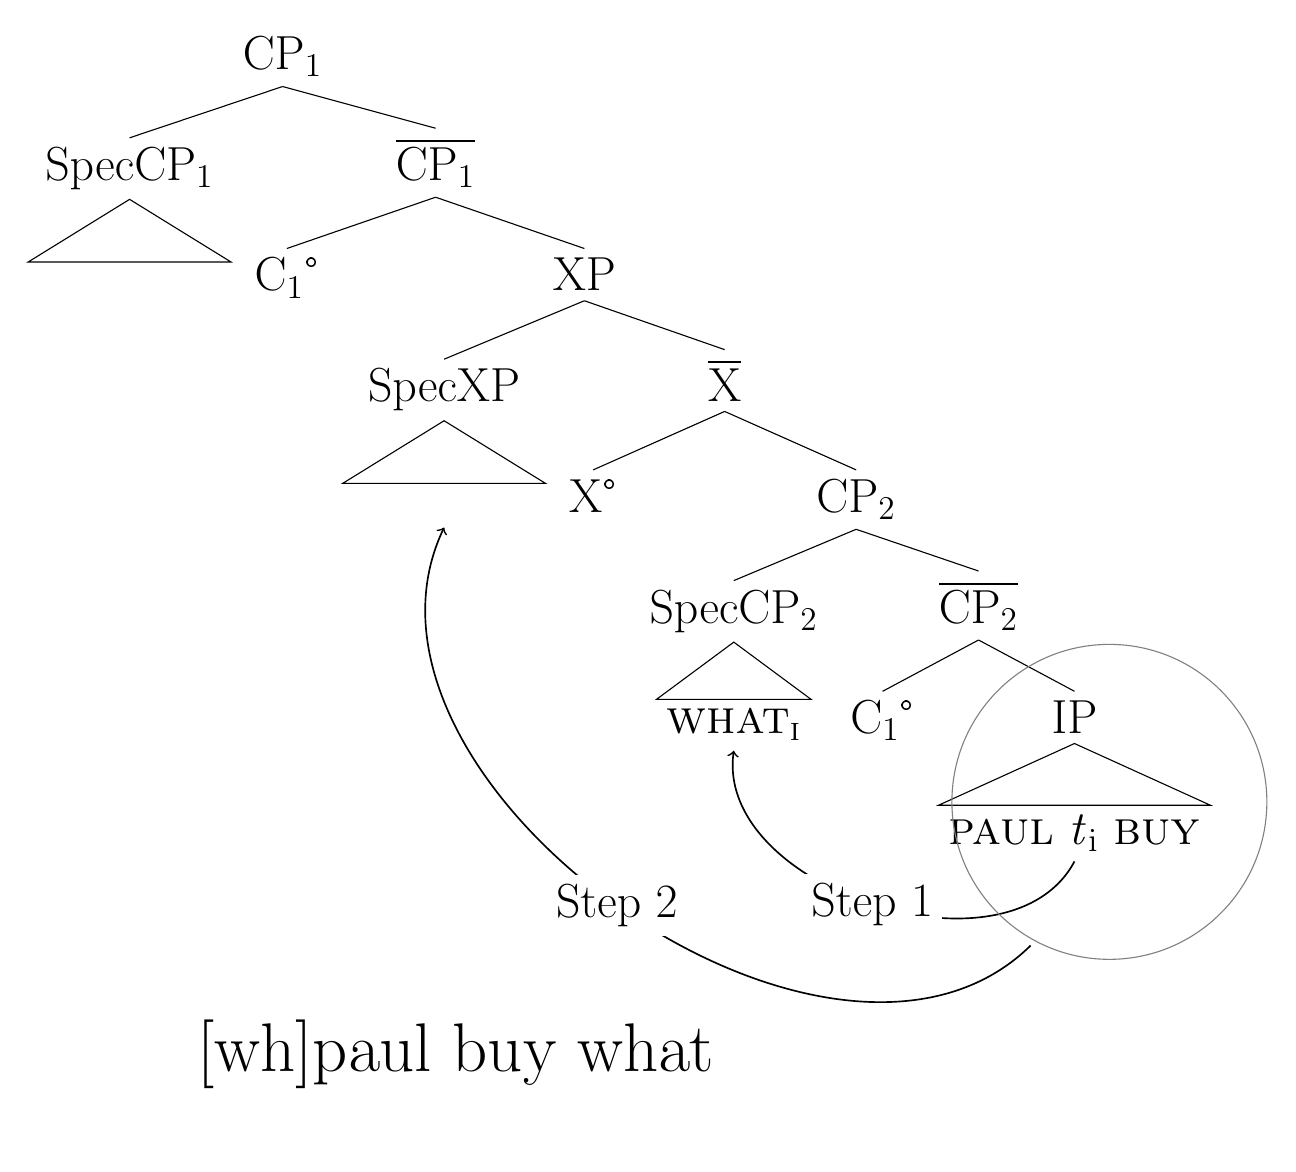
\begin{tikzpicture}[baseline]
\tikzset{level distance=40pt,sibling distance=5pt}
\Tree [.{\LARGE CP\textsubscript{1}} [.{\LARGE SpecCP\textsubscript{1}} \edge[roof]; \node(speccp1){\textcolor{white}{something here}}; ] [.{\LARGE $\overline{\textrm{CP\textsubscript{1}}}$} [.{\LARGE C\textsubscript{1}\textdegree} ] [.{\LARGE XP} [.{\LARGE SpecXP} \edge[roof]; \node(specintp){\textcolor{white}{something here}}; ] [.{\LARGE $\overline{\textrm{X}}$} [.{\LARGE X\textdegree } ] [.{\LARGE CP\textsubscript{2}} [.{\LARGE SpecCP\textsubscript{2}} \edge[roof]; \node(speccp2){\LARGE \textsc{what\textsubscript{i}}}; ] [.{\LARGE $\overline{\textrm{CP\textsubscript{2}}}$} [.{\LARGE C\textsubscript{1}\textdegree} ] [.{\LARGE IP} \edge[roof]; \node(ip){\LARGE \textsc{paul} $\textrm{\textit{t}}$\textsubscript{i} \textsc{buy}}; ] ] ] ] ] ] ]

\draw[semithick,->] (ip.south) to [bend right=-80] node [midway,fill=white] {\LARGE Step 1} (speccp2.south);
%\draw[semithick,->] (ip)..controls +(west:3) and +(south:4)..(speccp2);
\node (A) at (9.5,-11.0) {};
\draw[gray] (10.5,-9.3) circle (2cm);
\draw[semithick,->] (A.south) to [bend right=-80] node [midway,fill=white] {\LARGE Step 2} (specintp.south);
\node (text) at (2.2,-12.5) {\Huge \slg[wh]{paul buy what}};
%
%\node (overlinetext) at (3.5,-12.1) {wh};
%\node (text) at (2.2,-12.5) {$\overline{\textrm{\textsc{paul buy what}}}$};

\end{tikzpicture}
\end{adjustbox}
\ex\label{ex:firstanalysisbtwob}
\begin{adjustbox}{max width=0.46\textwidth}
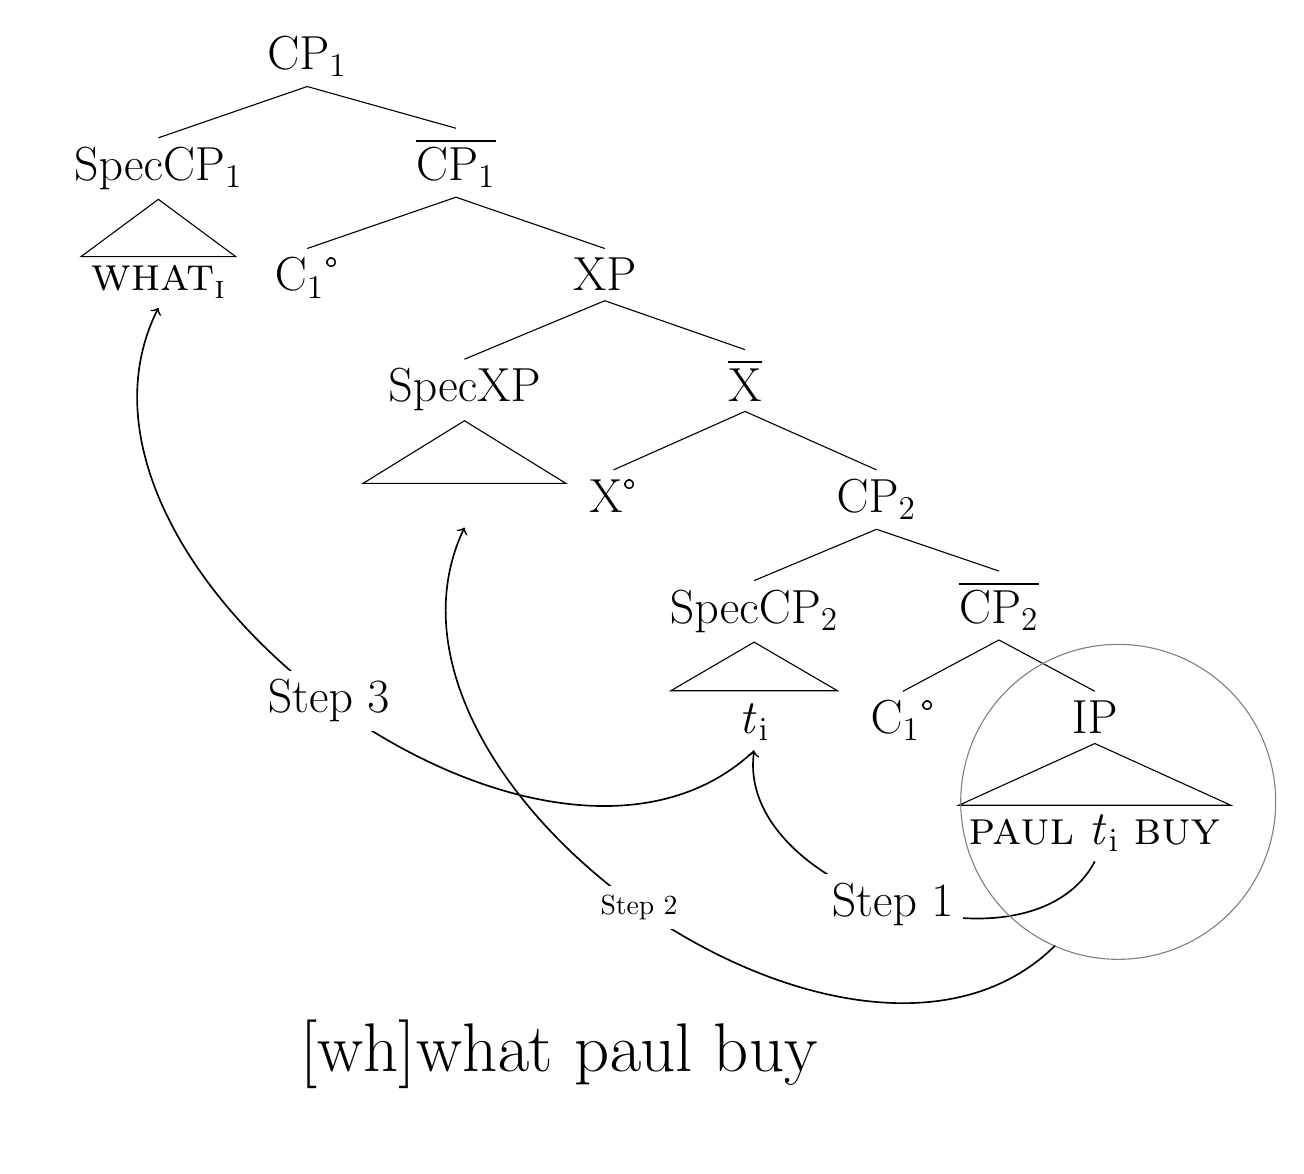
\begin{tikzpicture}[baseline]
\tikzset{level distance=40pt,sibling distance=5pt}
\Tree [.{\LARGE CP\textsubscript{1}} [.{\LARGE SpecCP\textsubscript{1}} \edge[roof]; \node(speccp1){\LARGE \textsc{what\textsubscript{i}}}; ] [.{\LARGE $\overline{\textrm{CP\textsubscript{1}}}$} [.{\LARGE C\textsubscript{1}\textdegree} ] [.{\LARGE XP} [.{\LARGE SpecXP} \edge[roof]; \node(specintp){\textcolor{white}{something here}}; ] [.{\LARGE $\overline{\textrm{X}}$} [.{\LARGE X\textdegree } ] [.{\LARGE CP\textsubscript{2}} [.{\LARGE SpecCP\textsubscript{2}} \edge[roof]; \node(speccp2){\LARGE \textcolor{white}{bla}\textit{t}\textsubscript{i}\textcolor{white}{bla}}; ] [.{\LARGE $\overline{\textrm{CP\textsubscript{2}}}$} [.{\LARGE C\textsubscript{1}\textdegree} ] [.{\LARGE IP} \edge[roof]; \node(ip){\LARGE \textsc{paul} $\textrm{\textit{t}}$\textsubscript{i} \textsc{buy}}; ] ] ] ] ] ] ]

\draw[semithick,->] (ip.south) to [bend right=-80] node [midway,fill=white] {\LARGE Step 1} (speccp2.south);
\draw[semithick,->] (speccp2.south) to [bend right=-80] node [midway,fill=white] {\LARGE Step 3} (speccp1.south);

\node (A) at (9.5,-11.0) {};
\draw[gray] (10.3,-9.3) circle (2cm);
\draw[semithick,->] (A.south) to [bend right=-80] node [midway,fill=white] {Step 2} (specintp.south);
\node (text) at (3.2,-12.5) {\Huge \slg[wh]{what paul buy}};
%\node (overlinetext) at (4.5,-12.1) {wh};
%\node (text) at (3.2,-12.5) {$\overline{\textrm{\textsc{what paul buy}}}$};
\end{tikzpicture}
\end{adjustbox}
\end{xlist}
\end{multicols}
\end{exe}

\vspace{-0.5cm}

\noindent Now, we need to account for clause-initial complex \textit{wh}-phrases. Again, this is an easy task, as they are simply base-generated in SpecCP\textsubscript{1}. This is shown in (\ref{ex:firstanalysisacomplex}). Left-branch extraction is shown in (\ref{ex:firstanalysisacomplexb}). Again, partial doubling with complex \textit{wh}-phrases can be seen as a combination of the two processes in (\ref{ex:firstanalysisacomplex}).
%\clearpage
\begin{exe}
\ex\label{ex:firstanalysisacomplex}
\begin{multicols}{2}
\begin{xlist}
\ex \label{ex:firstanalysisacomplexa}
\begin{adjustbox}{max width=0.46\textwidth}
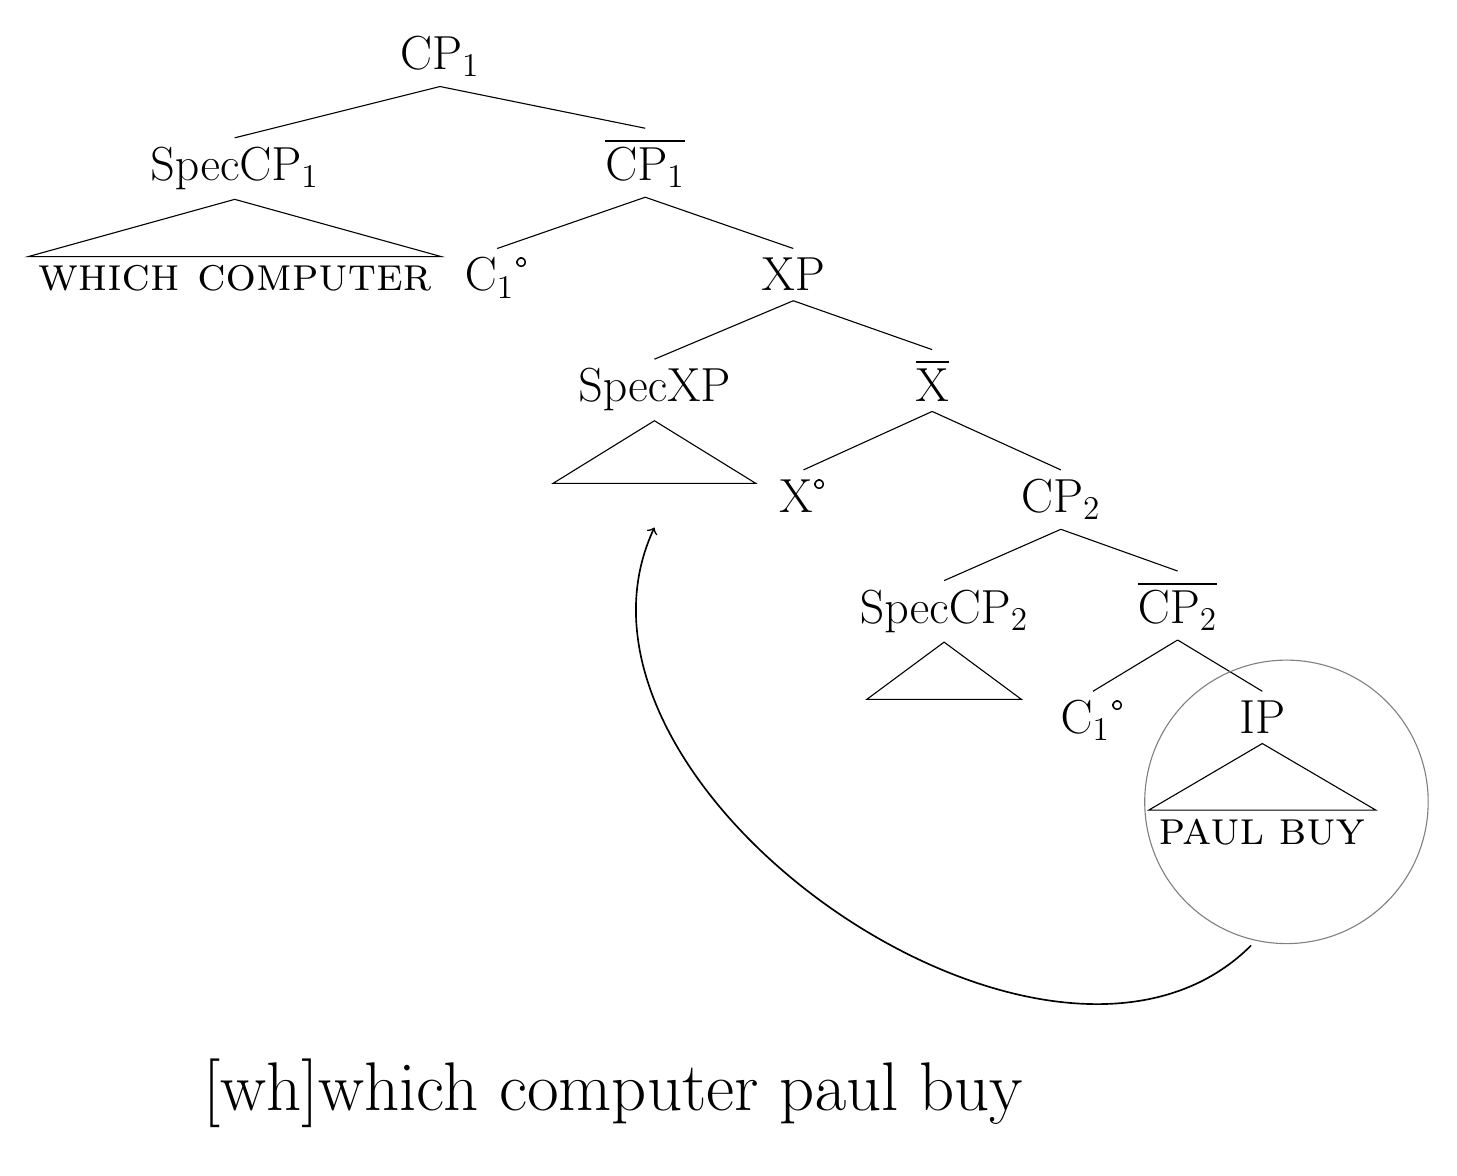
\begin{tikzpicture}[baseline]
\tikzset{level distance=40pt,sibling distance=5pt}
\Tree [.{\LARGE CP\textsubscript{1}} [.{\LARGE SpecCP\textsubscript{1}} \edge[roof]; \node(speccp1){\LARGE \textsc{which computer}}; ] [.{\LARGE $\overline{\textrm{CP\textsubscript{1}}}$} [.{\LARGE C\textsubscript{1}\textdegree} ] [.{\LARGE XP} [.{\LARGE SpecXP} \edge[roof]; \node(specintp){\textcolor{white}{something here}}; ] [.{\LARGE $\overline{\textrm{X}}$} [.{\LARGE X\textdegree } ] [.{\LARGE CP\textsubscript{2}} [.{\LARGE SpecCP\textsubscript{2}} \edge[roof]; \node(speccp2){\textcolor{white}{\LARGE \textsc{what\textsubscript{i}}}}; ] [.{\LARGE $\overline{\textrm{CP\textsubscript{2}}}$} [.{\LARGE C\textsubscript{1}\textdegree} ] [.{\LARGE IP} \edge[roof]; \node(ip){\LARGE \textsc{paul} \textsc{buy}}; ] ] ] ] ] ] ]

%\draw[semithick,->] (ip.south) to [bend right=-80] node [midway,fill=white] {Step 1} (speccp2.south);
%\draw[semithick,->] (ip)..controls +(west:3) and +(south:4)..(speccp2);
\node (A) at (10.3,-11.0) {};
\draw[gray] (10.75,-9.3) circle (1.8cm);
\draw[semithick,->] (A.south) to [bend right=-80] node [midway] {} (specintp.south);
\node (text) at (2.2,-13) {\Huge \slg[wh]{which computer paul buy}};
%\node (overlinetext) at (4.75,-12.1) {wh};
%\node (text) at (2.2,-12.5) {$\overline{\textrm{\textsc{which computer paul buy}}}$};

\end{tikzpicture}
\end{adjustbox}
\ex\label{ex:firstanalysisacomplexb}
\begin{adjustbox}{max width=0.46\textwidth}
\begin{tikzpicture}[baseline]
\tikzset{level distance=40pt,sibling distance=5pt}
\Tree [.{\LARGE CP\textsubscript{1}} [.{\LARGE SpecCP\textsubscript{1}} \edge[roof]; \node(speccp1){\textcolor{white}{\LARGE \textsc{computer}}}; ] [.{\LARGE $\overline{\textrm{CP\textsubscript{1}}}$} [.{\LARGE C\textsubscript{1}\textdegree} ] [.{\LARGE InterP} [.{\LARGE SpecInterP} \edge[roof]; \node(specintp){\textcolor{white}{something here}}; ] [.{\LARGE $\overline{\textrm{Inter}}$} [.{\LARGE Inter\textdegree } ] [.{\LARGE CP\textsubscript{2}} [.{\LARGE SpecCP\textsubscript{2}} \edge[roof]; \node(speccp2){\LARGE \textsc{which\textsubscript{i}}}; ] [.{\LARGE $\overline{\textrm{CP\textsubscript{2}}}$} [.{\LARGE C\textsubscript{1}\textdegree} ] [.{\LARGE IP} \edge[roof]; \node(ip){\LARGE \textsc{paul} $\textrm{\textit{t}}$\textsubscript{t} \textsc{computer buy}}; ] ] ] ] ] ] ]

%\draw[semithick,->] (ip.south) to [bend right=-80] node [midway,fill=white] {Step 1} (speccp2.south);
%\draw[semithick,->] (ip)..controls +(west:3) and +(south:4)..(speccp2);
\node (A) at (10.3,-10.9) {};
%\draw[gray] (10.3,-9.3) circle (1.8cm);
\draw[gray] (12.8,-9.3) ellipse (4cm and 1.8cm); %breite and höhe


\draw[semithick,->] (A.south) to [bend right=-80] node [midway] {} (specintp.south);
\node (text) at (2.2,-15) {\Huge \slg[wh]{paul computer buy which}};


%\node (overlinetext) at (4.68,-13.1) {wh};
%\node (text) at (2.2,-13.5) {$\overline{\textrm{\textsc{paul computer buy which}}}$};
\draw[semithick,->] (ip.south) to [bend right=-80] node [midway] {} (speccp2.south);


\end{tikzpicture}
\end{adjustbox}
\end{xlist}
\end{multicols}
\end{exe}


\noindent Real doubling of complex \textit{wh}-phrases is also disallowed in the model proposed in (\ref{ex:firstanalysisacomplex}) as there is only one host projection for complex \textit{wh}-phrases. 

As mentioned, there are several drawbacks in this second model as one needs to assume an additional layer of functional structure and additional movement steps that are hard to motivate. It shows, however, that it is possible to model the complex empirical data with this kind of model. On the whole, splitting up the CP following \citet{van2010complex, van2012you} seems to be a promising account for constituent interrogatives in sign languages. 

Before turning to imperatives in DGS, I will briefly describe some minor question types in DGS, namely alternative questions, tag questions, suggestive questions, and rhetorical questions. 

\section{Other types of interrogatives in DGS}\label{otherinterr}
While polar and constituent questions have received much attention in the sign language literature, other, non-canonical question types have been scarcely described. In this section, I will go through the following non-canonical interrogatives: alternative questions  (\ref{minorquestiontypesaa}), degree questions (\ref{minorquestiontypesdegree}), tag questions (\ref{minorquestiontypesa}), suggestive questions (\ref{minorquestiontypesd}), and (real) rhetorical questions (\ref{minorquestiontypese}).%\footnote{ Alternative questions are only sometimes } 

\begin{exe}
\ex\label{minorquestiontypes}\begin{xlist}
\ex Do you want beer, wine, or vodka? \hfill{\textit{Alternative question}} \label{minorquestiontypesaa}
\ex How big is your dog? \hfill{\textit{Degree question}} \label{minorquestiontypesdegree}
\ex Paul often buys cigarettes, doesn't he? \hfill{\textit{Tag question}} \label{minorquestiontypesa}
\ex Why don't we try something new?  \hfill{\textit{Suggestive question}}  \label{minorquestiontypesd}
\ex Do you want to miss this chance? \hfill{\textit{Rhetorical question}} \label{minorquestiontypese}




\end{xlist}
\end{exe} 


\noindent In each of the following subsections, I will briefly describe each question type and their expression in DGS.

\subsection{Alternative questions}
\is{alternative interrogatives|(}
Alternative question are similar to polar interrogatives as they refer to a choice. Alternative questions, however, cannot be answered by `yes' or `no', but require a different choice. The non-manual marking of alternative interrogatives in DGS does not differ from that of polar interrogatives, as shown in Figure (\ref{alternativequestion}) (similar to, for example, Italian Sign Language or Sign Language of the Netherlands as described in \citealt{brunelli2011antisymmetry}). The example in the figure, the translational equivalent of \textit{Do you like coffee, tea, or beer?}, shows that alternative interrogatives are marked by raised eyebrows and leaning forward and tilting the head. As was described for polar interrogatives, the intensity of the non-manuals increases towards the end. This is especially true for putting the head forward and tilting it.


\begin{figure}[bt]
\centering
	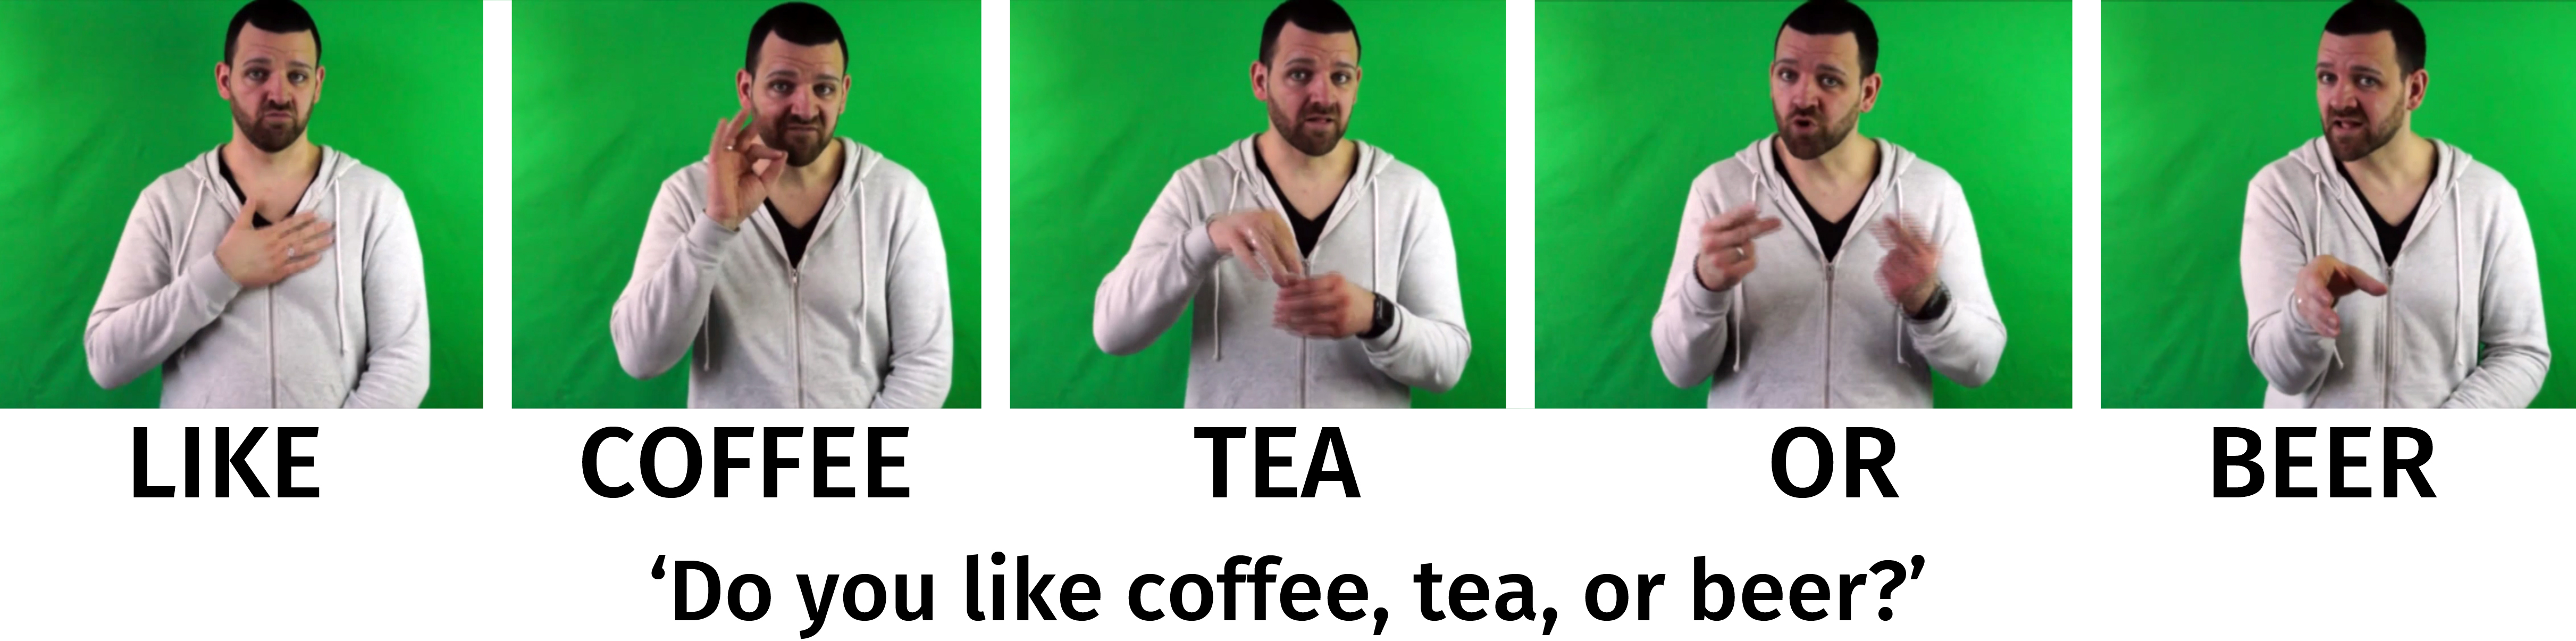
\includegraphics[width=1.0\textwidth]{alternativequestion.jpg}
	\caption{The non-manual markings used in alternative interrogatives are the same as in polar interrogatives. Note that the subject is dropped in the example and that the change in word order (VO instead of OV) is not due to the sentence being an alternative question, but is rather related to the verb being volitional.}
	\label{alternativequestion}
\end{figure}

\is{alternative interrogatives|)}


\subsection{Degree questions}
\is{degree interrogatives|(}
%\sub
Degree interrogatives are used to ask a question about the degree of a gradable property (e.\,g., \textit{How long is your hair?}). There is only scarce mention about this question type in the literature (e.\,g., \citealt{meier2001result, abrusan2011wh, tiemann2012crosslinguistic}). While questions are traditionally either divided into two major classes, polar and constituent interrogatives, or three classes, polar, constituent, and alternative interrogatives, it is possible that degree questions form a major class of their own. As almost nothing is known about degree questions I will only briefly discuss them here under the header of `other types of interrogatives'.

On the surface, spoken languages often encode degree questions as \textit{wh}-questions. This is, for example, the case in spoken German which makes use of the \textit{wh}-element \textit{wie} `how', as shown in (\ref{ex:germandegree}). 

\begin{exe}
\ex German \\ \gll {\textit{Wie}} {\textit{lang}} {\textit{sind}} {\textit{deine}} {\textit{Haare}?} \\
{how} {long} {are} {your} {hair} \\
\trans `How long is your hair?' \label{ex:germandegree}
\end{exe} 


\noindent Other languages, in contrast, have their own strategies to express degree questions. In Mandarin Chinese, for example, the degree particle \textit{duo} `many' is used to express degree questions, as shown in (\ref{ex:chinesdegree}).


\begin{exe}
\ex Mandarin \\ \gll {\textit{nide}} {\textit{toufa}} {\textit{you}} {\textit{duo}} {\textit{chang}} \\
{you.\textsc{rel}} {hair} {have} {many} {long} \\
\trans `How long is your hair?' \label{ex:chinesdegree}
\end{exe} 

\noindent The only mention of this question type in the literature on DGS, as far as I am aware, is found in \citet[335]{happ2014vork} who label it `million alternatives questions' as the answer set of alternatives is theoretically infinite \citep{fox2006universal}. DGS has its own strategy to encode this question type. To form a degree question, the signer produces the sign denoting the property in different degrees. This is illustrated in (\ref{ex:millionalternativequestion}). The non-manuals used with degree questions do not differ from those used with polar questions, as shown in Figure (\ref{millionalternativequestions}).

\begin{exe}
\ex \slg[degree]{poss_2 dog big(1) big(2)}
%{\hspace{103pt}degree}  \\
%{$\overline{\textrm{\textsc{poss}\textsubscript{2} \textsc{dog big(1) big(2)}}}$}
\glt `How big is your dog?' \label{ex:millionalternativequestion}
\end{exe}


\begin{figure}[bt]
\centering
	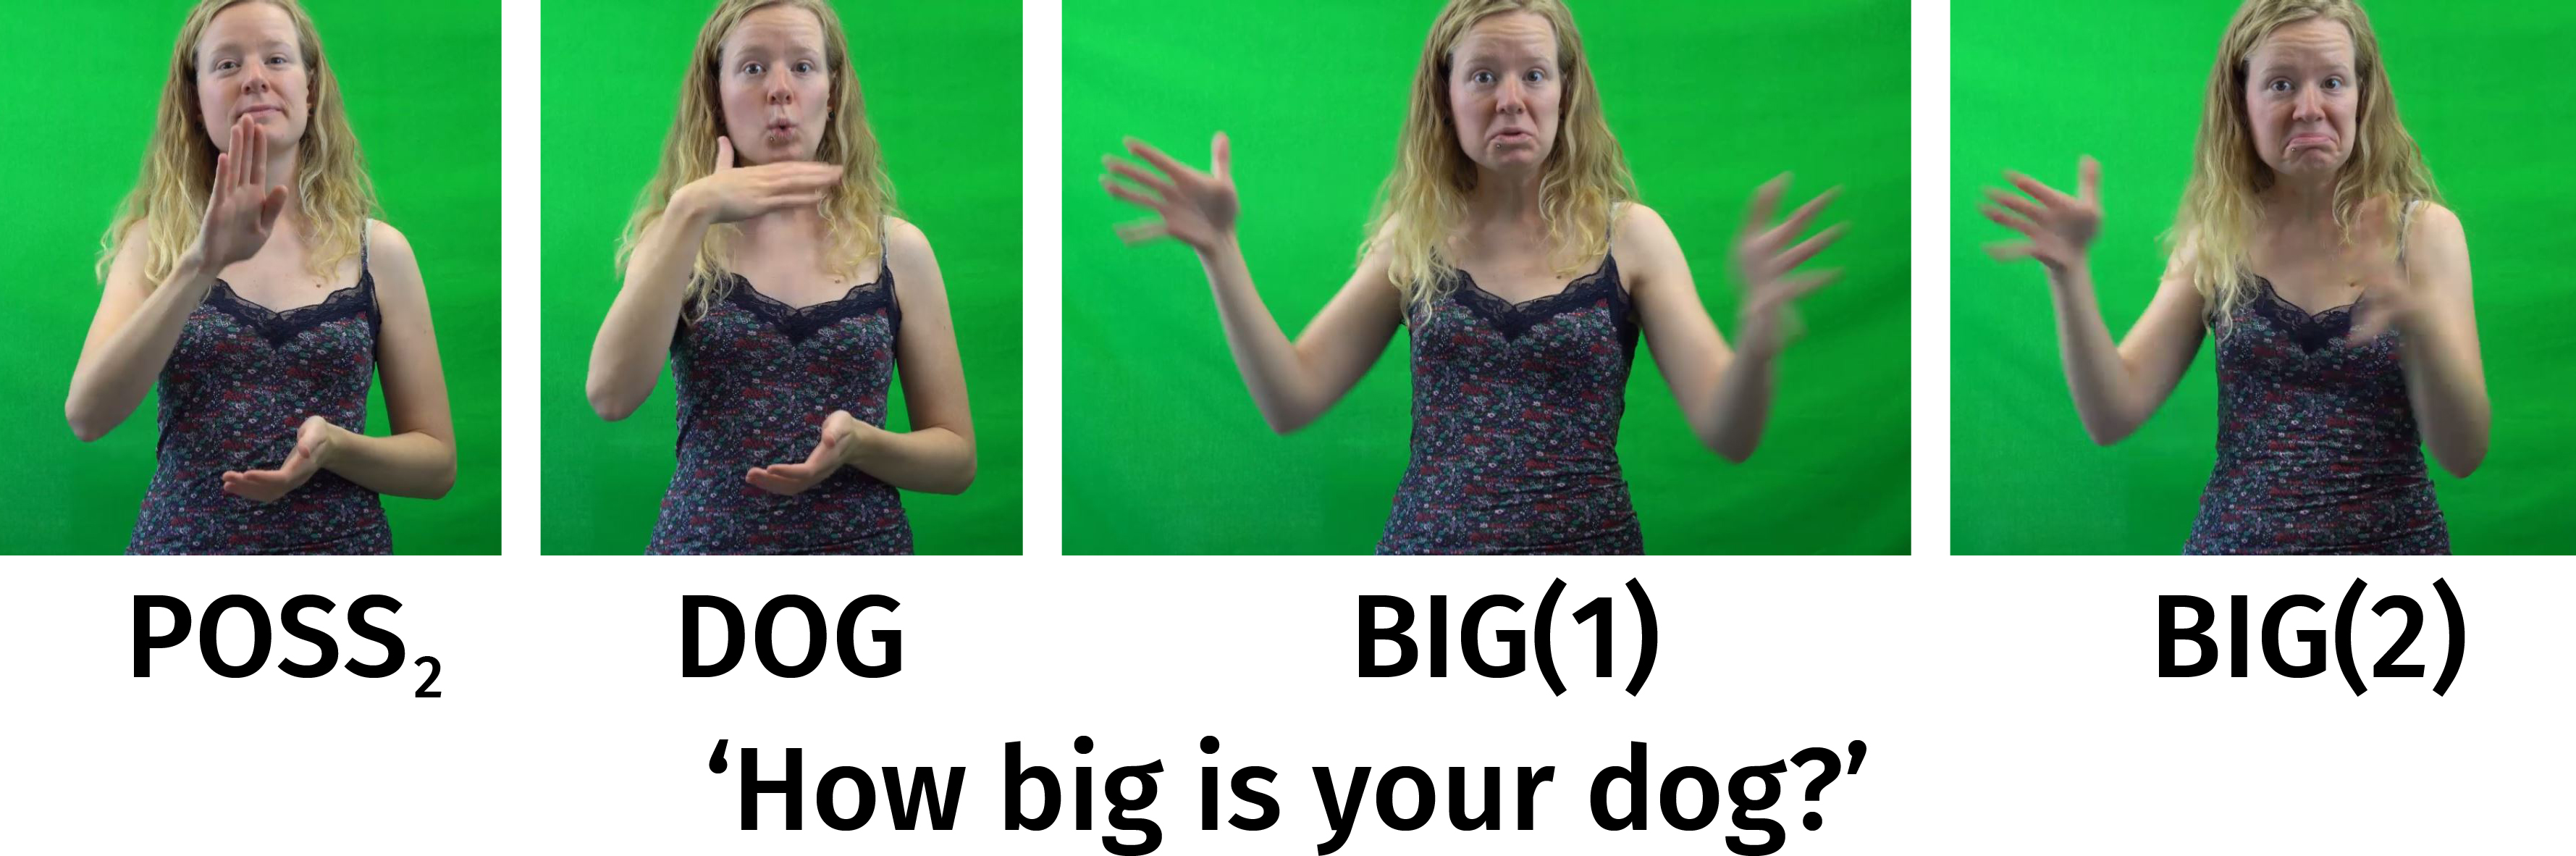
\includegraphics[width=1.0\textwidth]{millionalternativequestions.jpg}
	\caption{Example of a degree question in DGS. Note that the signer pulls her mouth angles down towards the end of the sentence. This seems to be an optional (and thus gestural) non-manual expressing that the signer is missing some information.  }
	\label{millionalternativequestions}
\end{figure}

\is{degree interrogatives|)}

\subsection{Tag questions}
\is{tag questions|(}\is{question tag|see{tag question}}
Tag questions, i.\,e., yes/no interrogatives used when the speaker/signer suddenly becomes uncertain about a proposition s/he felt sure about previously and is seeking the hearer's support along the way, are produced using the tag sign \textsc{right} or its negative pendant \textsc{right-neg}. The non-manuals of a regular polar question and the non-manuals of a tag question are the same (which is expected, as tag questions, in fact, are polar interrogatives). This means that the eyebrows are raised and the head is put forward and tilted. These non-manuals, again, are strongest clause-finally. However, there is a clear pause before the question tag and the tag itself may be accompanied by a head nod. This is illustrated in Figure \ref{tagquestion}.

\begin{figure}[bt]
\centering
	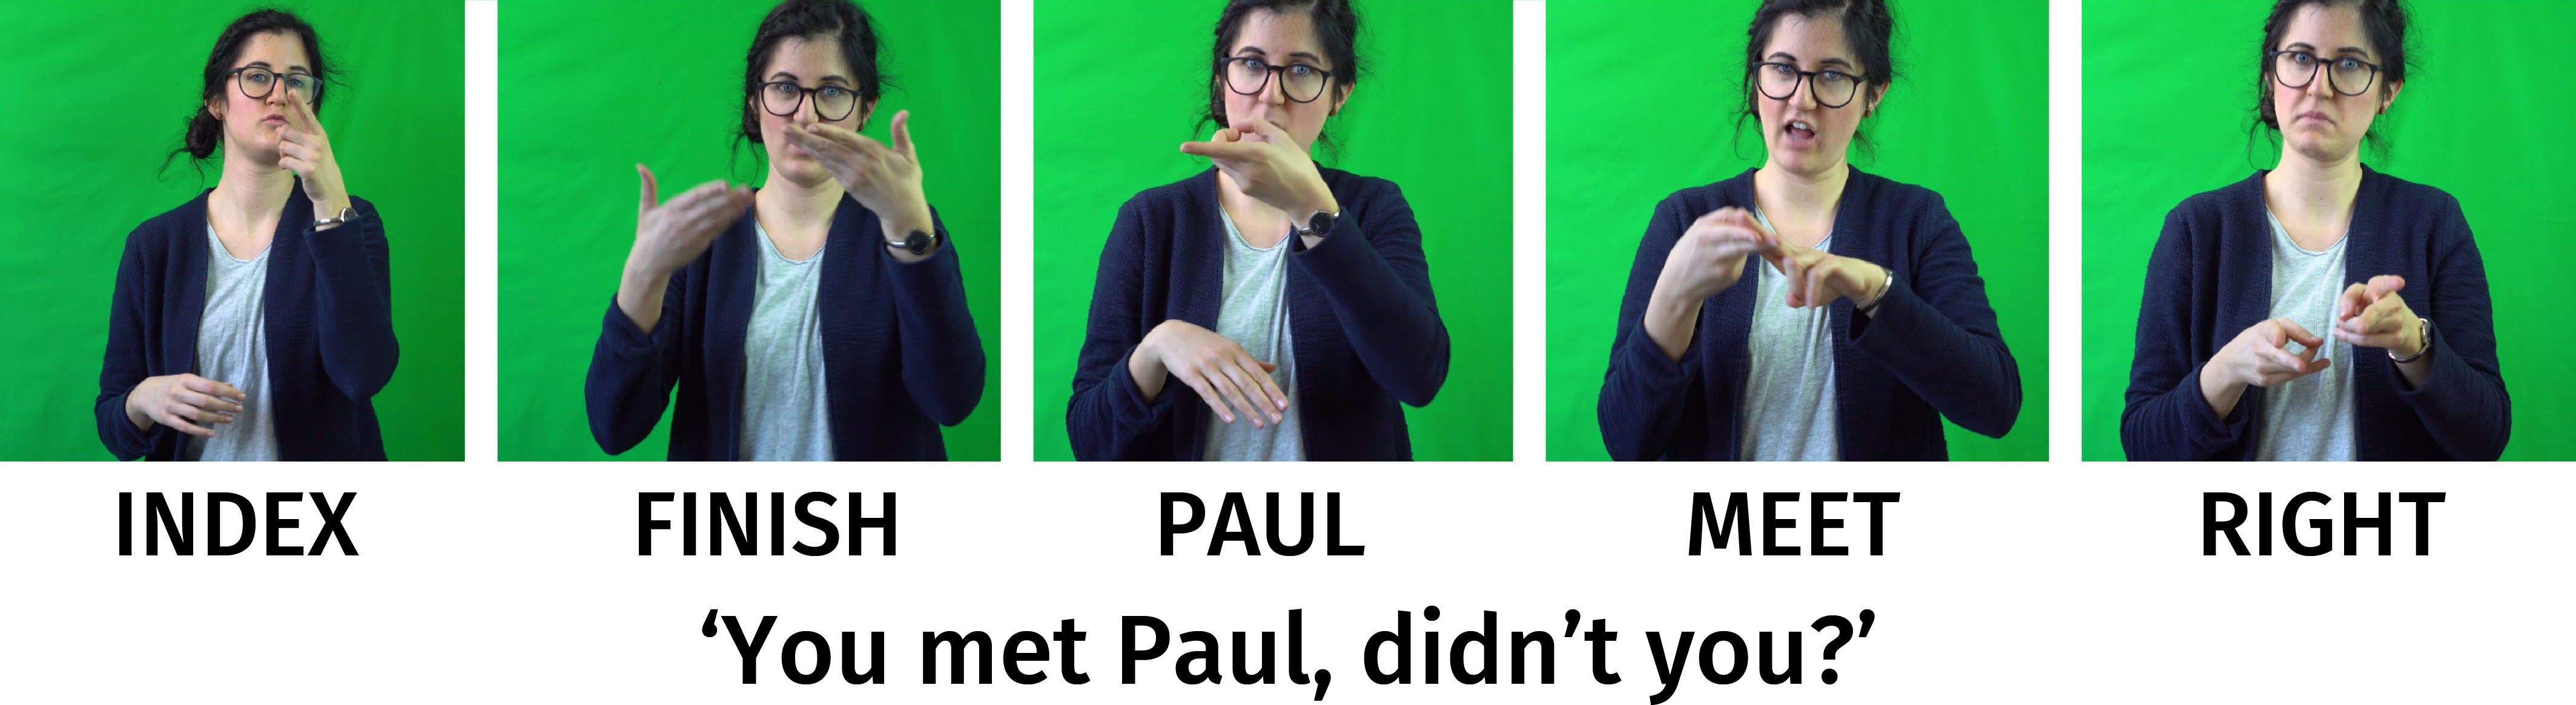
\includegraphics[width=1.0\textwidth]{tagquestion.jpg}
	\caption{The non-manuals used in tag question do not differ from polar questions. The tag itself is preceded by a clear intonational break and the question tag is accompanied by a head nod. Note that in this example, the sign \textsc{finish} appears as a perfect marker.}
	\label{tagquestion}
\end{figure}

\is{tag questions|)}


\subsection{Suggestive questions}
\is{suggestive questions|(}
Interrogatives used as suggestions and especially \textit{why-not}-questions are of special interest because this type of interrogative is superficially very similar to \textit{wh}-interrogatives, with the difference that \textit{why-not}-questions are not used as real information-seeking questions. I have found no restrictions as to the landing site of the \textit{wh}-phrase with suggestive questions although the clause-internal position seems to be preferred (i.\,e., the \textit{wh}-sign is left \textit{in-situ}). A typical example looks like the one in (\ref{ex:suggquest}). 

\begin{exe}
\ex \slg[sugg-wh]{today why not vegetarian cook}
%{\hspace{158pt}sugg-wh}  \\
%{$\overline{\textrm{\textsc{today why not vegetarian cook}}}$}
\glt `Why don't we cook something vegetarian today?' \label{ex:suggquest}
\end{exe}

\noindent The most important difference between real information-seeking questions and suggestive questions is of non-manual nature. As shown in Figure \ref{suggquest}, lowered and squinted eyebrows as the common markers of \textit{wh}-questions are nearly absent in suggestive questions. Additionally, the eyes are more open. This observation supports the idea that the eyebrows play a major role in clause-typing. 

\begin{figure}[bt]
\centering
	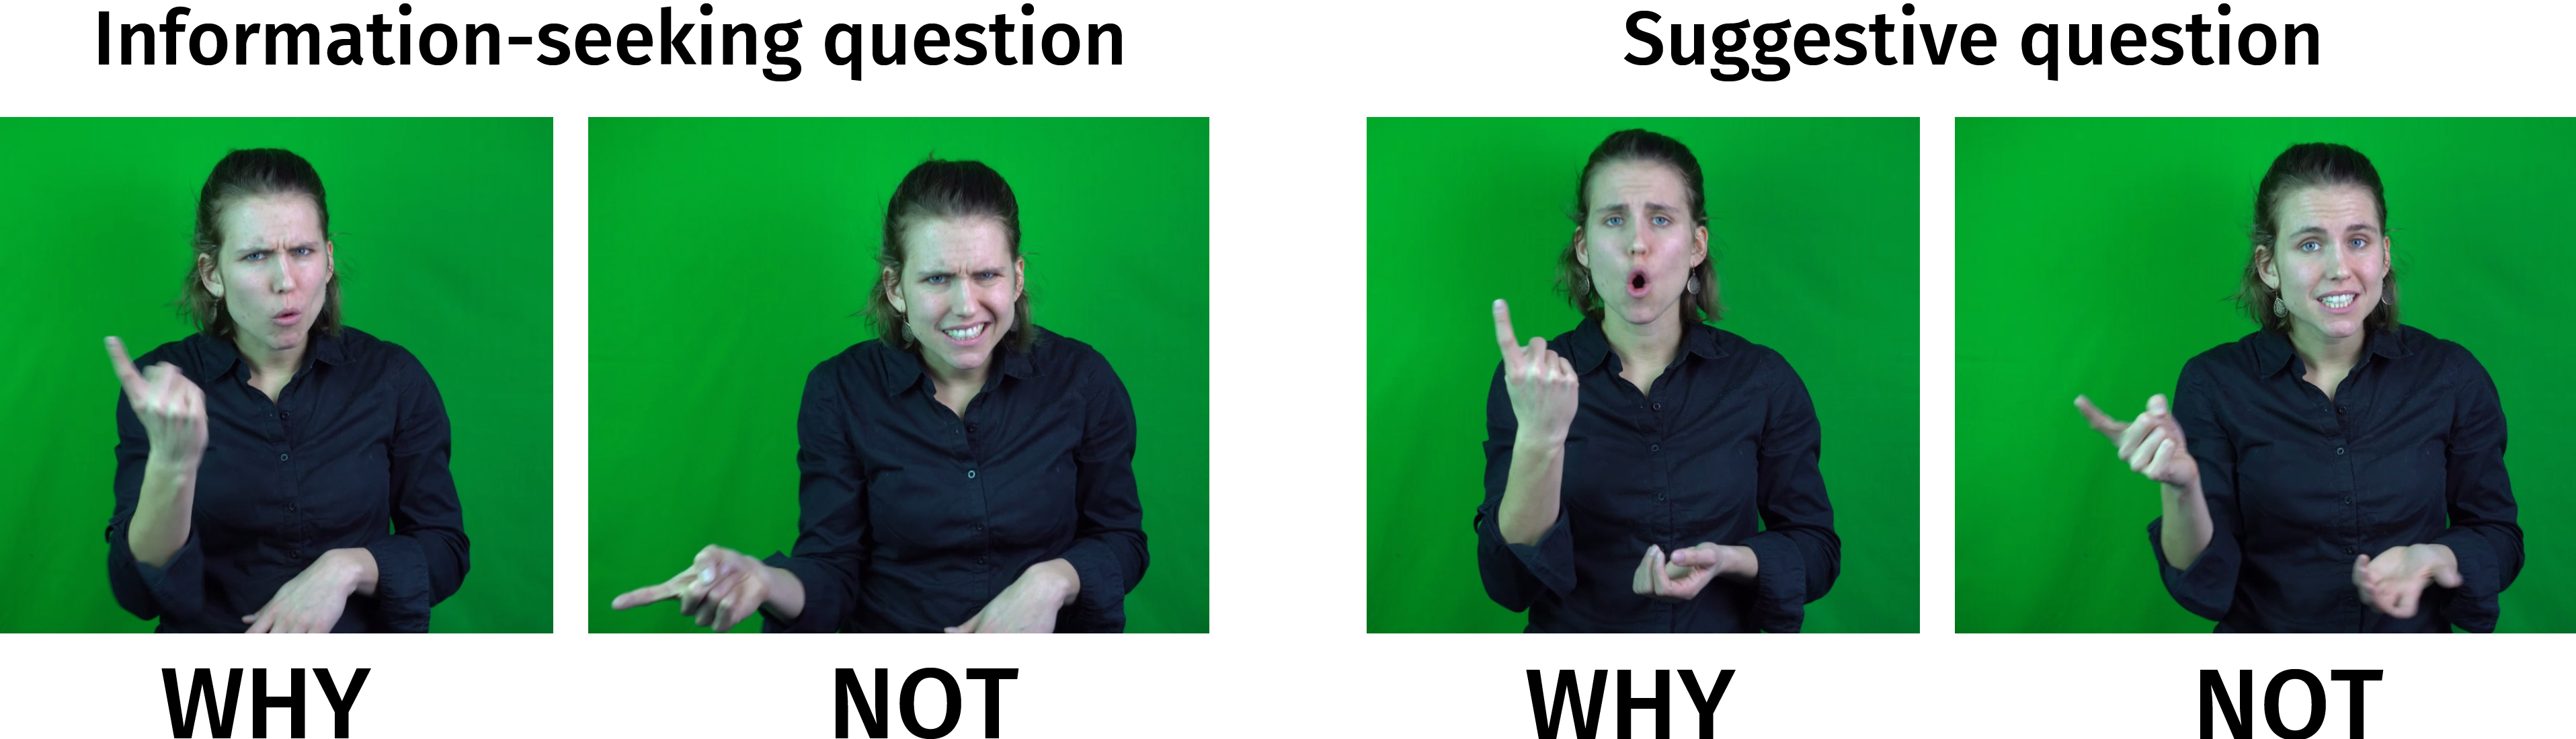
\includegraphics[width=1.0\textwidth]{suggquest.jpg}
	\caption{Non-manual differences between information-seeking and suggestive questions. }
	\label{suggquest}
\end{figure}



\is{suggestive questions|)}

\subsection{Rhetorical questions}\label{rhetq}
\is{rhetorical question|(}
I will now turn to the discussion of rhetorical questions. A question is interpreted as being rhetorical when the answer to the question is in the common ground of the interlocutors \citep{caponigro2007rhetorical}. In other words, the hearer needs to be able to reconstruct the answer to the question \citep{truckenbrodt2004strukturbedeutung}. Rhetorical questions can be realized as polar or constituent interrogatives. Examples, including the re-constructable answers, are given in (\ref{rhetquestspoken}). 

\begin{exe}
\ex\label{rhetquestspoken}\begin{xlist}
\ex Do you want to miss this chance? \\
\textasciitilde You do not want to miss this chance. \label{polarrhet}
\ex Who likes rocket salad? \\
\textasciitilde Nobody likes rocket salad. \label{constituentrhet}
\end{xlist}
\end{exe} 

\noindent Note that the rhetorical questions in (\ref{rhetquestspoken}) are used to make statements. There are, however, other speech acts that can be performed with rhetorical questions, e.\,g.,  accusations (\textit{Why do you always act like a child?}). 

The question of how rhetorical questions are formed in sign language has not received much attention in previous research. Most of the research concerns question-answer pairs, such as the one from \citet[138]{baker1980american} in (\ref{ex:bakercokely}) (with `rq' meaning rhetorical question). I will not discuss this use as it may be better analyzed as an instance of pseudo-clefting (e.\,g., \citealt{wilbur1996evidence}; see also the discussion starting from page \pageref{pseudocleeeeefts}).%\footnote{ Thus, the translation of the example in (\ref{ex:bakercokely}) would rather be something like: `Why the woman died is because she refused to eat.'}(note that the structures discussed here are `real' rhetorical questions and not pseudo-clefts as discussed starting from Page \pageref{pseudocleeeeefts} which are also sometimes called `rhetorical' in the literature)

\begin{exe}
\ex American Sign Language\\ \slg{woman die,} \slg[rq]{why,} \slg{refuse eat}
%{} {\hspace{86pt}rq} {} \\
%{\textsc{woman die,}} {$\overline{\textrm{\textsc{why}}}$,} {\textsc{refuse eat}}
\glt `This woman died, because she refused to eat.' \label{ex:bakercokely} 
\end{exe}

\noindent Instead, I will briefly describe how real rhetorical questions are formed in DGS. Rhetorical questions are of special interest concerning the non-manual markers used in DGS questions. In Section \ref{polarinterrogativesdgs} and Section \ref{whinterrogativedgs}, I have argued that each of the three non-manual markers in DGS interrogatives has a meaning on its own. To be more precise, I claimed that raising the eyebrows is the general marker of a polar question and lowering the eyebrows is used to mark constituent interrogatives, that putting the head forward signals that the signer is expecting an answer/reaction, and that tilting the head siedways is used to express epistemic commitment (see also Section \ref{perhapsmoodirrealis}). 

These claims can be tested with rhetorical questions. As rhetorical questions are still questions, we would expect the eyebrow marking to be present in both polar and constituent rhetorical questions. As the asker knows the (expected) answer in a rhetorical question we would expect putting the head forward to be absent. The same prediction can be made for tilting the head sideways as there should be no epistemic insecurity about the proposition expressed. 

\citet[333]{happ2014vork} discuss rhetorical constituent interrogatives in DGS and claim that they are marked by raised instead of lowered eyebrows. However, they define rhetorical questions as questions in which the person who asks the question knows the answer and only give examples from classroom contexts in which a teacher asks a question. As a teacher asking an examination question does know the answer, this type of question falls under their definition.

Educational questions asked in examination contexts are, although they are not to be considered as real rhetorical questions, of special interest as the circumstances in which they are being used are highly interesting. With an educational question, the asker knows the answer, but is still expecting an answer. We thus would expect the head being put forward, but expect the sideways tilt being absent. As shown in Figure \ref{educational}, this is indeed the case. With the educational constituent question shown in the figure, the signer raises her eyebrows, as described by \citet{happ2014vork}. As expected, the signer's head is straight, but put forward towards the end of the clause in the figure.\footnote{ It could be speculated that educational constituent interrogatives are a special kind of alternative question with the alternatives being the correct and the incorrect answers. This way, the raised eyebrows can be explained.}

\begin{figure}[bt]
\centering
	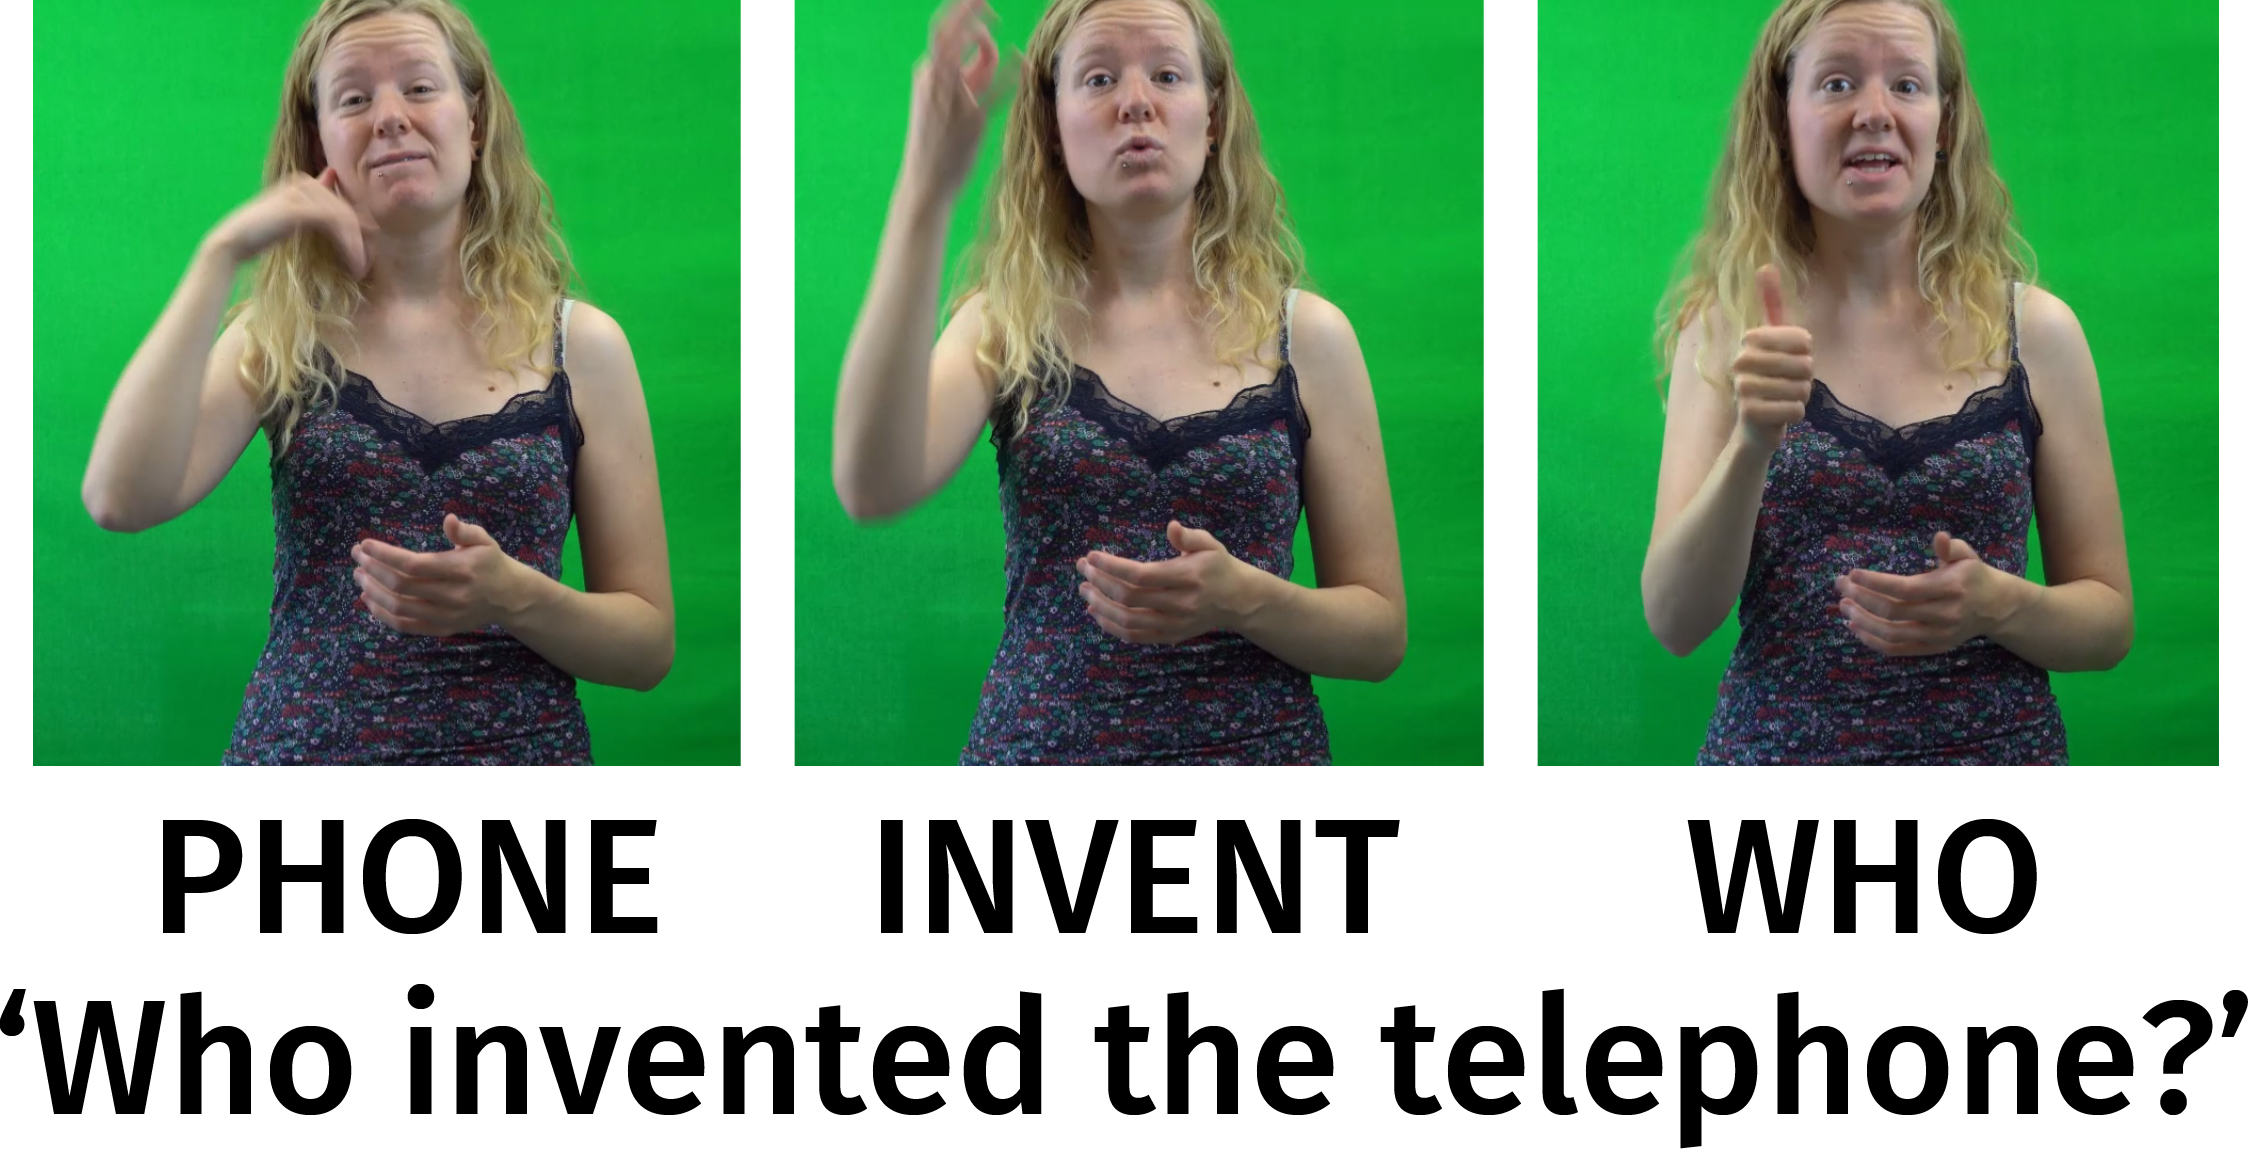
\includegraphics[width=1.0\textwidth]{educational.jpg}
	\caption{Educational constituent interrogatives can be accompanied by raised instead of lowered eye-brows.}
	\label{educational}
\end{figure}

Other types of rhetorical questions, however, receive different eyebrow markings and I argue that there is no uniform marking of rhetorical questions in DGS in the sense that there is one non-manual marker for this question type. In many cases, rhetorical questions are marked by furrowed brows. This is especially true for accusations, as shown in Figure \ref{accusation}. As can be seen from the example, the signer leans back towards the end of the sentence to signal that she is not sympathetic with the behavior of the addressee -- this non-manual, however, is not part of the rhetorical question, but of the speech act of accusing.

\begin{figure}[bt]
\centering
	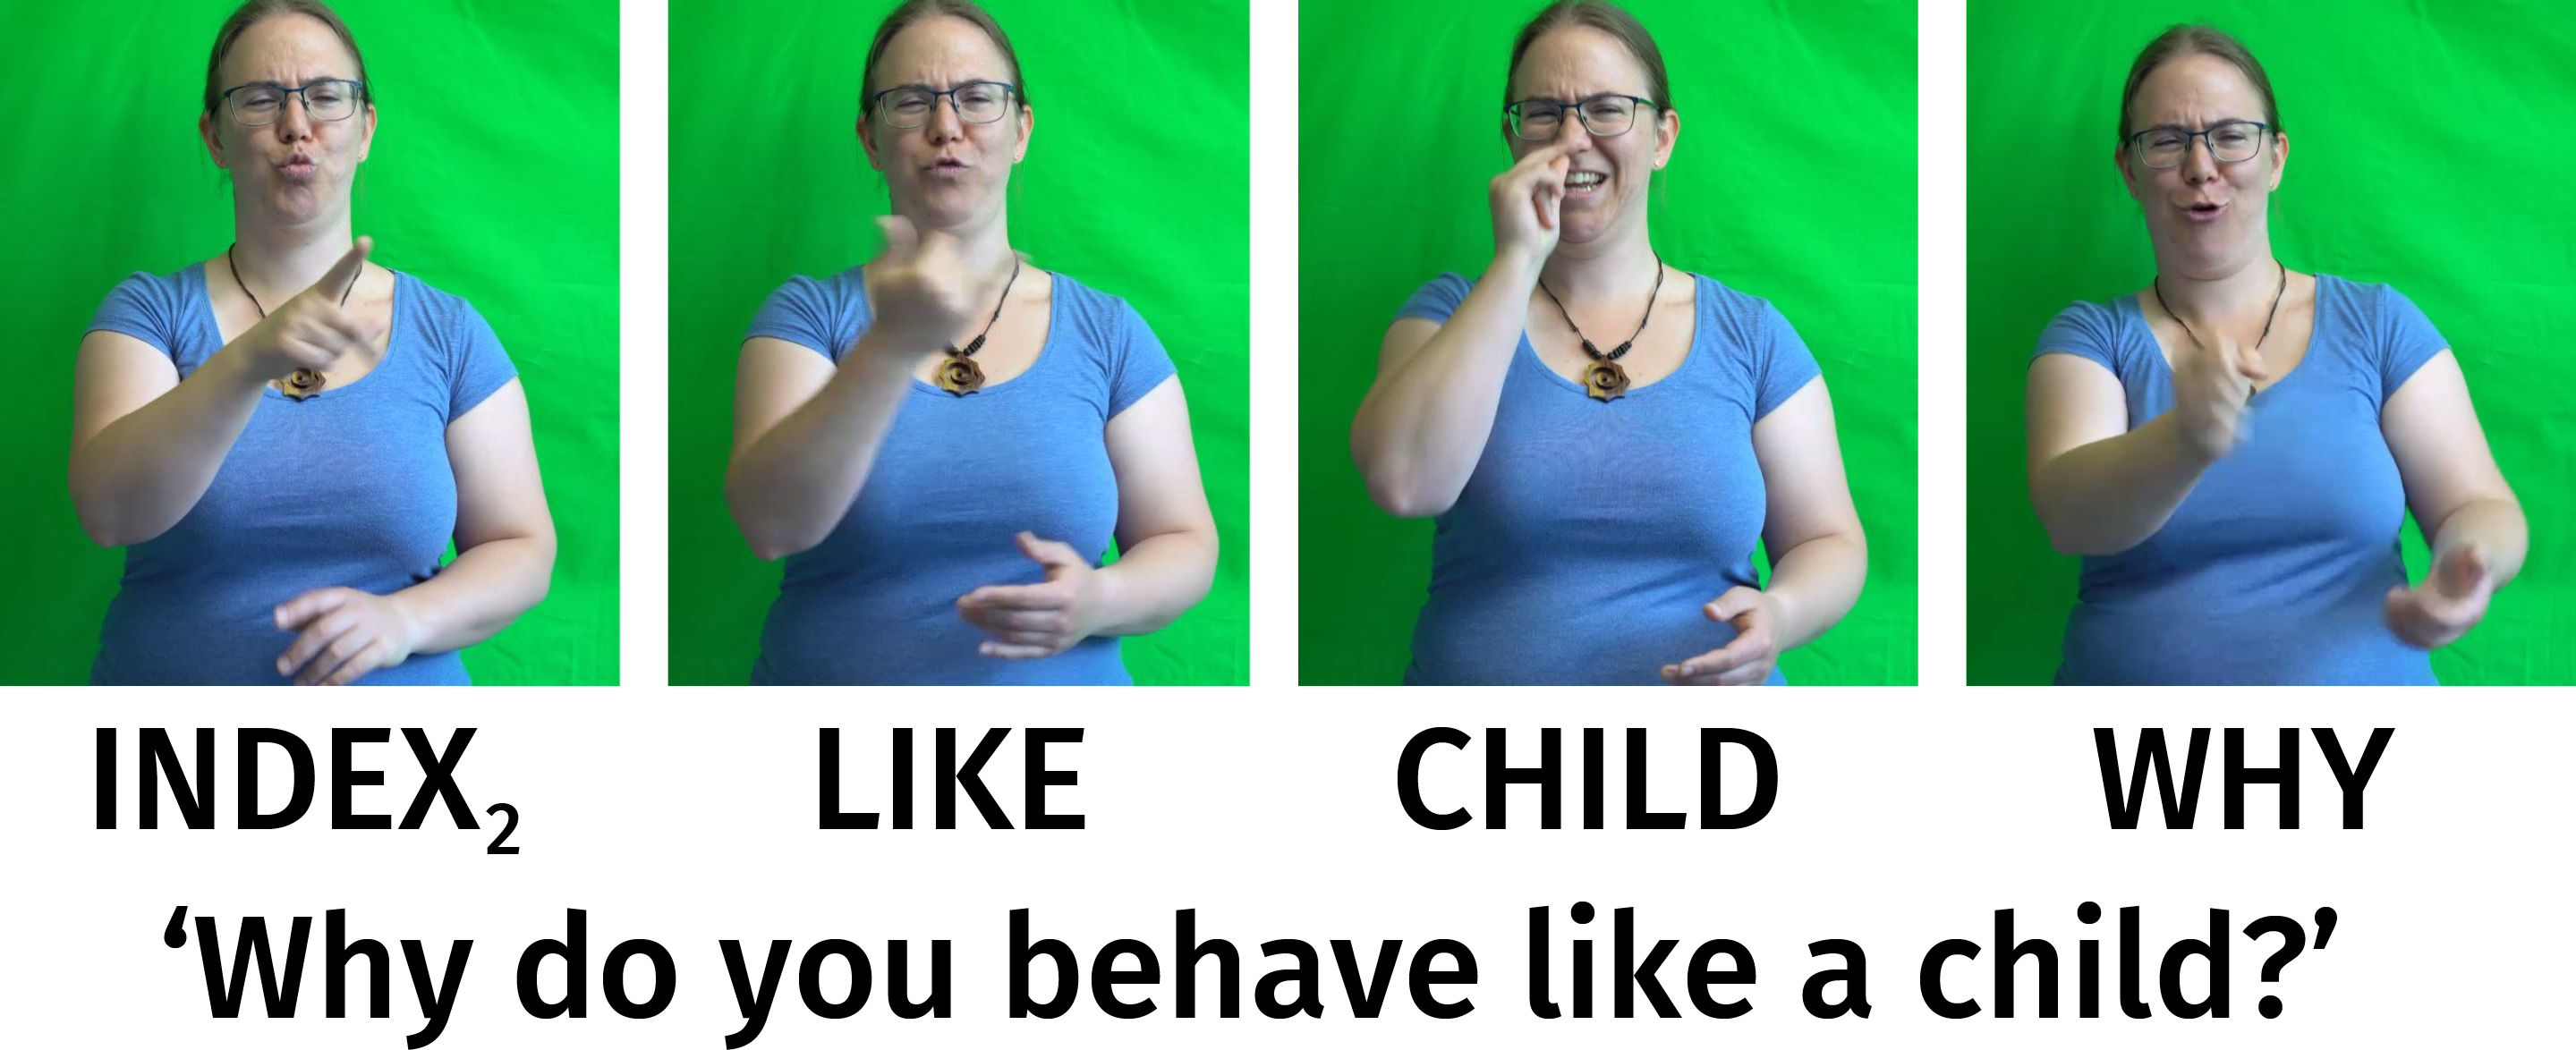
\includegraphics[width=1.0\textwidth]{accusation.jpg}
	\caption{Rhetorical questions used as accusations receive furrowed brows.}
	\label{accusation}
\end{figure}

The non-manuals for rhetorical questions that are used as statements are subject to variation. It seems as if rhetorical questions with negative re-constructable answers receive a brow-furrow. This is illustrated for a rhetorical content and a rhetorical polar question in Figure \ref{rhetorical}. Note that in both cases, the head is in a straight position and not put forward -- as the signer does know the answer and does not expect a response from the addressee. Additionally, rhetorical questions can be followed by a palm-up gesture, as shown in the figures. Note that the impression that the signer tilts her head sidewards comes from the fact that the palm-up gesture is accompanied by a head-shake (to indicate that the expected answer is no). 

\begin{figure}[bt]
\centering
	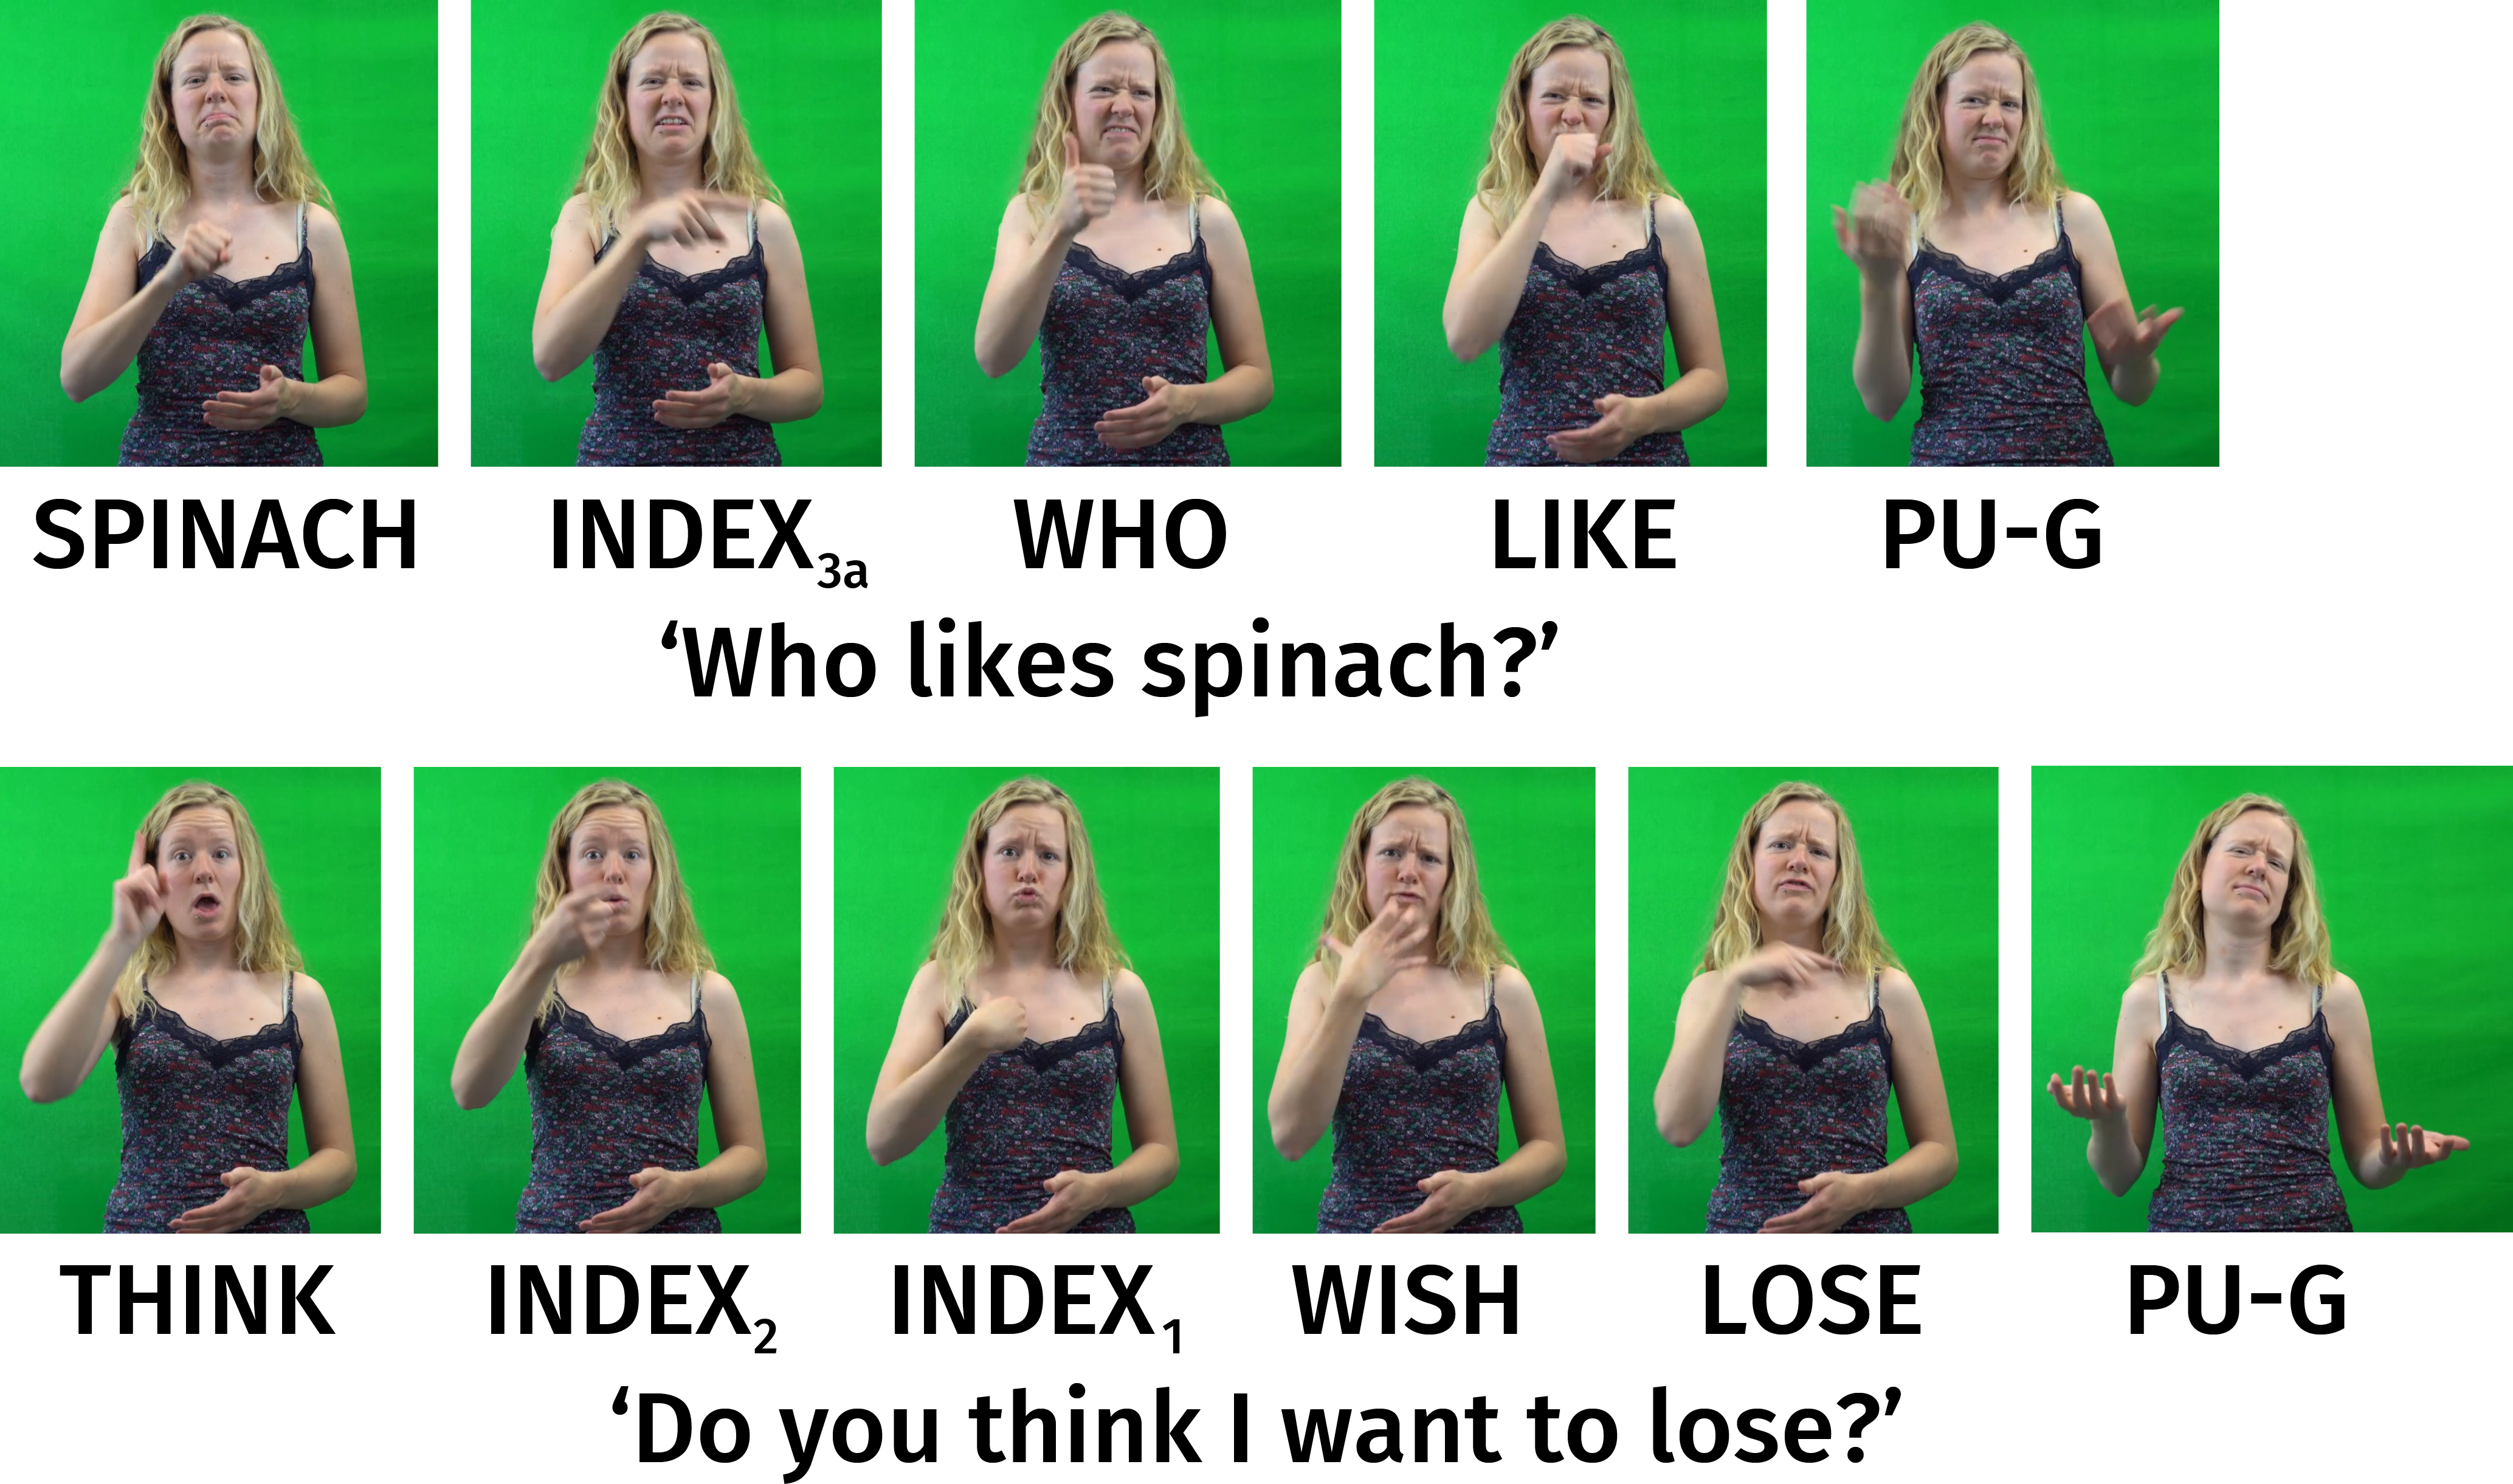
\includegraphics[width=1.0\textwidth]{rhetorical.jpg}
	\caption{Rhetorical questions expressing negative statements are marked with furrowed brows.}
	\label{rhetorical}
\end{figure}
%\clearpage
Rhetorical questions used as statements with positive re-constructable answers seem to receive eyebrow raise. This is shown using the example \textit{Don't we all want to be loved?} (triggering the positive re-constructable answer `Yes, we all want to be loved'), in Figure \ref{rhetlove}. Again, the head is held straight and not tilted to the side. 

\begin{figure}[bt]
\centering
	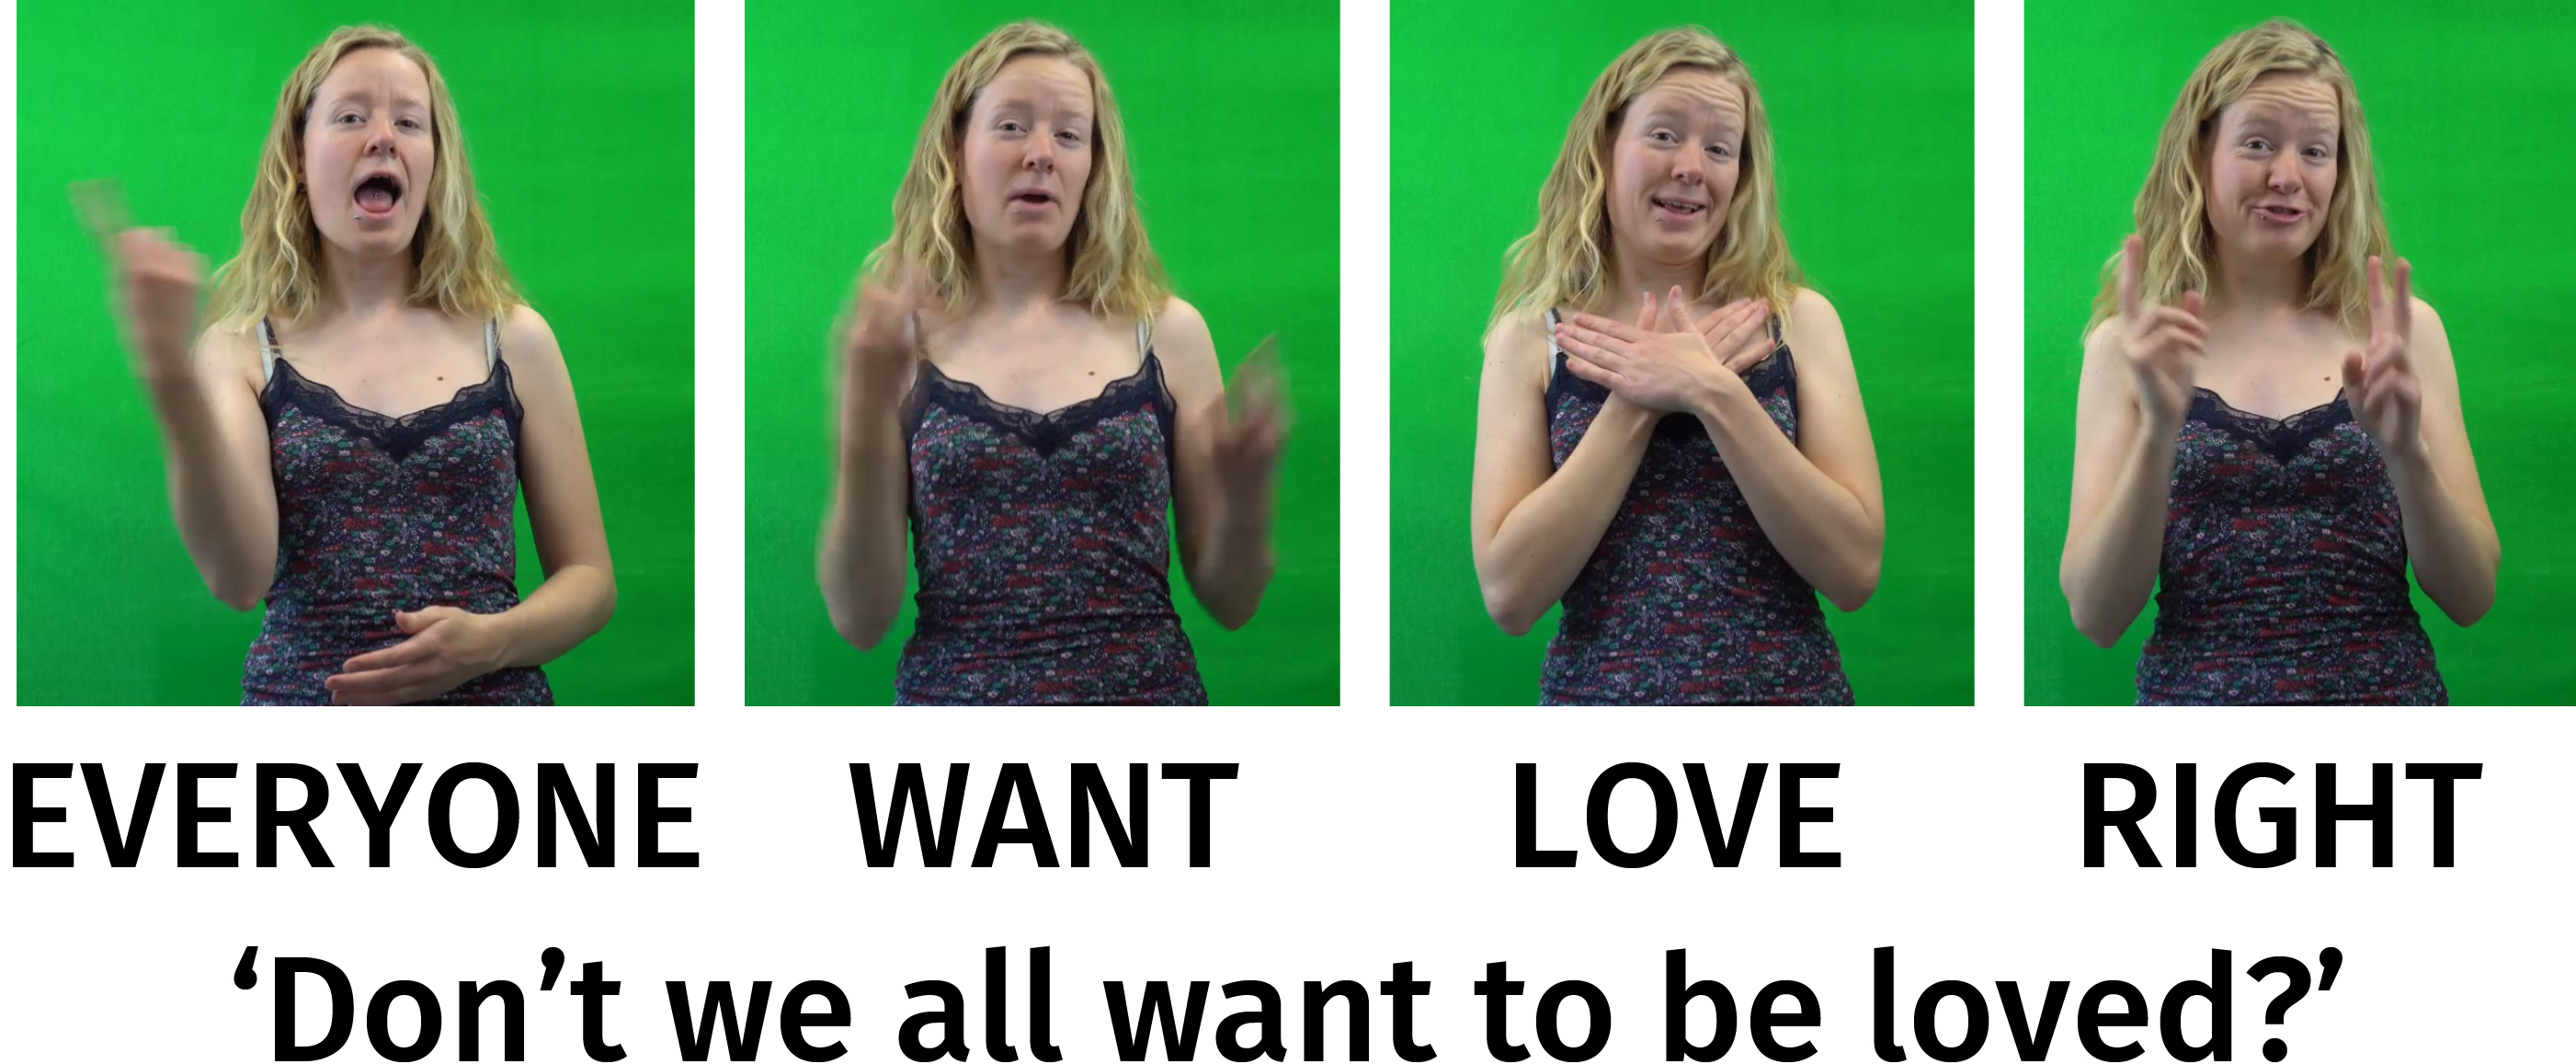
\includegraphics[width=1.0\textwidth]{rhetlove.jpg}
	\caption{Rhetorical questions expressing positive statements are marked with raised brows.}
	\label{rhetlove}
\end{figure}

Taken together, rhetorical questions receive non-manual markings with the eyebrows. The exact non-manuals depend on the answer to be reconstructed. 

\is{rhetorical question|)}

\section{Imperatives}\label{generalsectionimperatives}
\is{imperatives|(}
As in the previous sections, I will begin this section with a discussion of the general features of the phenomenon in spoken languages, followed by an overview over the sign language literature. Finally, I will go through the DGS data. I will show that the main marker of imperatives are the eyebrows, again with an intensity peak towards the end of the clause. In summary, the syntactic analysis of imperatives presented will not differ much from polar interrogatives: I assume that with imperatives, feature checking in a high CP projection takes places, triggering the non-manual markings -- the responsible head is either right-headed or left-headed with the whole clause being moved to a left-branching specifier. Besides the non-manuals, I will briefly discuss subject drop, the agreement behavior of verbs in imperative sentences, and negation in imperatives. 

\subsection{General overview}
Imperative sentences are sentences that are (typically) used for the communicative function of an order or request, i.\,e. the speaker/signer wants the addressee to carry out an action. An often cited definition of the prototypical meaning of an imperative is by \citet[212]{schmerling1982imperatives} who characterizes an imperative as ``an attempt to bring about a state of affairs in which the proposition expressed by the imperative is true''. This, however, downplays the importance of the addressee \citep[31]{van2007imperatives}. Although it covers orders, requests, and wishes, it does not say anything about who is addressed and if the attempt is realistic or not. It covers, for example, optatives of the sort \textit{May you live 100 years} that should not be covered by the term imperative. Additionally, this definition would cover promises such as \textit{In the future, I will never go to bed so late!} The missing part of Schmerling's definition is that the one who uses an imperative has the intention that the addressee adds the proposition expressed by the imperative to his/her to-do list in \citeauthor{portner2004semantics}'s (\citeyear{portner2004semantics}) terminology. Summarizing Generative analysis of imperatives, \citet[32]{van2007imperatives} concludes that the core meaning of an imperative is to get the ``addressee to bring about a state of affairs''. 

The prototypical directive is a command \citep[1--2]{aikhenval2010imp} although imperatives can be used for a variety of other directive speech acts as several authors stress. \citet[213]{clark1996using}, for example, notes:

\begin{quote}
A simple imperative like ``Sit here,'' for instance could be used as a command, request, offer, advisory or exhortation, depending on the context, as is shown by the following potential responses: ``Yes, sir'' (command), ``Okay'' (request), ``No thanks'' (offer), ``What a good idea'' (advisory), ``Thank you'' (exhortation).
\end{quote}

\noindent As noted already in Section \ref{sec:speechacts} (see page \pageref{threesources}) we need to be careful with the notions of sentence types, sentence mood, and the force of an utterance. The force of an utterance is inferred by a hearer from a combination of three sources: the context, the mood as encoded by syntax and the proposition expressed. Although imperatives like \textit{Sit here!}, \textit{Open the window!}, or \textit{Lie on the floor!} can be understood as a command, request, etc. in different contexts, without politeness markers it is understood as a command when no context is present and not as a request, offer, advisory, or exhoration (although it is often stressed the imperative mood is more flexible as it can express more speech-acts than other sentence moods, e.\,g., \citealt{portner2004semantics}; \citealt{kaufmann2012terpreting}).

Imperative sentences show a set of cross-linguistically stable properties. In the following I will briefly discuss three of these properties as they are either of interest when it comes to sign languages or are telling when it comes to the syntax of imperatives: (i) subject drop, (ii) the minimal verbal morphology found in imperatives, and (iii) the behavior of negation in imperatives. 

The first property of imperative sentences I will elaborate on is that they cross-linguistically allow for subject-drop -- even in languages that otherwise do not allow null-subjects (e.\,g., \citealt{alcazar2014syntax}). Broadly speaking, that the subject can be dropped in imperatives is due to the fact that the subject of an imperative is the addressee who is, under normal circumstances, present in the context of utterance. Although it seems as if there is no language that does not have the option for a non-overt subject in imperatives (e.\,g., \citealt{sadock1985speech}) there are good reasons to believe that imperatives nevertheless have a non-overt second person subject (\citealt{zwicky1988subject, potsdam1996syntactic} and the summary in \citealt[33--34]{van2007imperatives}). The major piece of empirical evidence for this assumption is that it is possible to bind a reflexive pronoun, as in (\ref{bindinga}).

\begin{exe}
\ex Introduce yourself! \label{bindinga}
\end{exe} 

\noindent As a reflexive pronoun like \textit{yourself} in (\ref{bindinga}) always needs to be bound we need to ask what its binder is. The only possibility here is that it is a second person subject referring to the addressee.

The second property of imperatives I briefly want to discuss is the cross-lingustically stable minimal verb morphology. Although there is a wide range of languages that employ special inflections to mark imperatives -- even including \is{reduplication}reduplications, as, for example, in Hopi \citet{benett1981} -- there is a strong tendency to use as minimal inflection as possible (just the verb root in the extreme case). \citet[172--173]{sadock1985speech}, for example, report that approximately half of their sample of 23 languages make use of no affixes at all. A related property of imperatives that has been noted to be cross-linguistically stable is the lack of tense-marking (e.\,g., \citealt{sadock1985speech}).

From the fact that many languages only show minimal verbal morphology in imperatives and the fact that tense-marking seems to be absent, many authors concluded that the structural make-up of imperatives is somehow impoverished. This is in line with the observation that it is not possible to embed imperatives \citep[78]{katz1964theory} and that there seems to be no language with imperative complementizers \citep[281]{konig2007speech}. However, it is not exactly clear which structures are missing in imperatives. For some authors, the TP is missing in imperatives (e.\,g., \citealt{zanuttini1991syntactic}) and for others it is FinP (e.\,g., \citealt{platzack1998subject}). Against the assumption that imperatives lack a TP altogether \citet{jensen2007favour} argued that the TP encodes the time of the utterance in this sentence type. On her account, it is the CP that is missing in imperatives. Yet other accounts assume that the TP/IP and the CP are fused into one projection in imperatives (e.\,g., \citealt{wratil2005syntax}).

Thus, there is general agreement on the impoverished syntax of imperatives, but not on its exact nature. However, most authors agree on the idea that there has to be an imperative sentence mood feature in the C domain (e.\,g., \citealt{rivero1995imperatives, zanuttini1997negation, platzack1998subject, potsdam2007analysing}), although there is no agreement on its exact position. The most natural assumption, at least in my mind, is to assume an imperative projection that should be understood as an analogon to the InterP (i.\,e., an ImpP). 

The third property I want to discuss briefly is the behavior of negative imperatives. Cross-linguistically there seem to be three strategies. Some language negate imperatives just as others sentence types, some languages use different negators, and others cannot use imperative verb morphology in negated imperatives. 

An example of the first class of languages is German. Thus, German negates imperatives in the same way as other sentence types as illustrated in (\ref{negimperativegerman}). 

\begin{exe}
\ex German\label{negimperativegerman}
\begin{xlist}
\ex {\gll {Ich} {esse} {das} {nicht.}\\
{I} {eat.\textsc{2sg}} {that} {not} \\
\trans `I don't eat that.' \label{negimperativegermabbbbaaa} \hfill\textit{Negative declarative} }
\ex {\gll {Iss} {das!}\\
{eat.\textsc{imp.sg}} {that} \\
\trans `Eat this!' \label{negimperativegermab} \hfill\textit{Imperative} }
\ex {\gll {Iss} {das} {nicht!}\\
{eat.\textsc{imp.sg}} {that} {not} \\
\trans `Don't eat this!' \label{negimperativegermac} \hfill\textit{Negative imperative} }
\end{xlist}
\end{exe}

\noindent The German examples show that in this language, declaratives are negated by the use of \textit{nicht} (\ref{negimperativegermabbbbaaa}). The same particle is used to negate imperatives, as shown by the non-negated (\ref{negimperativegermab}) and the negated imperatives (\ref{negimperativegermac}). Thus German uses the same negation strategy in imperatives as in other sentence types.% it is no problem to use the regular negator \textit{nicht} with an imperative verb form. 

Languages of the second class use different negators in imperatives than in other sentence types. Languages of this class are the American Indian language Yokuts, Old Greek, or Latin. This strategy is exemplified for Latin in (\ref{negimplat}).

\begin{exe}
\ex Latin\label{negimplat}
\begin{xlist} 
\ex \gll {\textcolor{white}{*}Non} {constat.}\\
{\textcolor{white}{*}not} {certain\textsc{3sg.pres}} \\
\trans \textcolor{white}{*}`It is not certain.' \hfill{\textit{Negative declarative}} \label{negimplata}
\ex \gll {\textcolor{white}{*}Ne} {puero} {gladium!}\\
{\textcolor{white}{*}not} {boy.\textsc{dat}} {sword.\textsc{acc}} \\
\trans{\textcolor{white}{*}`Don't give a boy a sword!' \hfill{\textit{Negative imperative}}}\label{negimplatb}
\ex \gll {*Non} {puero} {gladium!}\\
{\textcolor{white}{*}not} {boy.\textsc{dat}} {sword.\textsc{acc}} \\
\trans \textcolor{white}{*}`Don't give a boy a sword!' \hfill{\textit{Negative imperative}}\label{negimplatc} 

\end{xlist}
\end{exe} 

\noindent As can be seen from the examples, Latin uses the negator \textit{non} in declaratives (\ref{negimplata}) (and interrogatives), but has to resort to the negator \textit{ne} in imperatives (\ref{negimplatb}) and (\ref{negimplatc}). 

Finally, other languages resort to the strategy of not using an imperative verb morphology in negative imperatives. This strategy is illustrated for Spanish in the examples in (\ref{negimperativespanish}) from \citet[57--58]{van2007imperatives}.

\begin{exe}
\ex Spanish \citep[57--58]{van2007imperatives}\label{negimperativespanish}
\begin{xlist}
\ex[\textcolor{white}{*}] {\gll Lee!\\
read.\textsc{imp.sg} \\
\trans `Read!' \label{negimperativespanisha} \hfill{\textit{Imperative}} }
\ex[*] {\gll {No} {lee!}\\
{not} {read.\textsc{imp.sg}} \\
\trans `Don't read!' \label{negimperativespanishb} \hfill{\textit{Negative imperative}} }
\ex[\textcolor{white}{*}] {\gll {No} {leer}\\
 {Not} {read.\textsc{inf}} \\
\trans `Don't read!' \label{negimperativespanishc} \hfill{\textit{Negative imperative (infinitive)}}}
\ex[\textcolor{white}{*}] {\gll {No} {leas!}\\
 {Not} {read.\textsc{pres.subj.2sg}} \\
\trans `Don't read!' \label{negimperativespanishd} \hfill{\textit{Negative imperative (subjunctive)}}}
\end{xlist}
\end{exe}

\noindent In Spanish, the verb has a special imperative morphology, as shown in the glosses in (\ref{negimperativespanisha}). If an imperative sentence is negated, it is not possible to just combine the regular negator \textit{no} and the verb in its imperative form (\ref{negimperativespanishb}), but rather the verb has to be either in the infinitive (\ref{negimperativespanishc}) or in the subjunctive (\ref{negimperativespanishd}). 

Although there are different explanations for this variation, all (standard) analyses have in common is that they assume there is an imperative-specific movement process \citep{zanuttini1991syntactic, rivero1994negation, rivero1995imperatives, platzack1998subject, zeijlstra2004sentential}. On most accounts it is assumed that in imperatives, the verb has to move to check an imperative feature, that is located in the left periphery (e.\,g., in C\textdegree\ for Rivero \& Terzi or in Mood\textdegree\ for Zanuttini and Zeijlstra). In affirmative imperatives this can be achieved through cyclic head movement. In the first type of account, this movement is blocked due to an intervening NegP between VP and CP \citep{rivero1994negation, rivero1995imperatives} and in the second type of account this movement is blocked, in some languages, due to the structural make-up of the NegP and its position (e.\,g., \citealt{zeijlstra2004sentential}).

That some languages allow for regular negators in imperatives is, in some accounts, explained by assuming that in these languages the verb does not need to move to the left periphery to check the imperative feature because there is a special clitic position in these languages that is licensed by C\textdegree . This means that C\textdegree\ in these languages cannot bear the imperative feature and the verb checks this feature lower down in the structure. Therefore, it is no problem for a NegP to intervene. However, as noted by \citet[62]{van2007imperatives}, empirically this cannot be on the right track as the languages allowing regular negation in imperatives and the languages with this special kind of clitic position do not coincide. Additionally, it is unclear why one should assume that the imperative feature in affirmative and negative imperatives can be checked in two different structural positions with different syntactic heights. 

The basis of the second account is the observation that the position of the NegP (hosting negation), in stark contrast to other functional projections, seems to vary -- from language to language, but also within a single language when it comes to different negators \citep{ouhalla1990sentential, ouhalla1991functional, zanuttini1991syntactic}. Additionally, negators can sometimes be in a head and sometimes in a specifier position. As the structure of imperative clauses is impoverished, as discussed above, some languages featuring a higher NegP cannot express negation in a regular way in negative imperatives since the relevant host structure for this NegP is missing (TP for \citealt{zanuttini1991syntactic} or FinP for \citealt{platzack1998subject}). In languages in which NegP is located lower down in the structure, there is no problem as its host structure is still present in imperatives. For \citet{zeijlstra2004sentential}, languages fall into two classes: the negator is either located in the head of a NegP (e.\,g., Spanish) or it is realized as a vP adjunct (e.\,g., German). When the negative marker is located in Neg\textdegree , as in Spanish, movement of the verb into a higher position, more precisely to Mood\textdegree , is blocked due to the head movement constraint. When the negator is located in the vP adjunct position, Neg\textdegree\ remains phonologically empty (still bearing an uninterpretable negative feature) and does not block movement. 

\subsection{Imperatives in sign languages}

\subsubsection{Non-manual markers}
Comparatively little is known about imperatives in sign languages. The available descriptions, however, clearly indicate that the main marker of imperatives are non-manual in nature. For many sign languages, this seems to be done with the eyebrows. In Italian Sign Language the non-manuals consist of furrowed brows and tensed eyes, in Catalan Sign Language furrowed brows, and in French Sign Languages raised eyebrows \citep{donati2017searching} (for Italian Sign Language see also \citealt{brunelli2011antisymmetry}). The same source (i.\,e., \citealt{donati2017searching}) mentions that Icelandic, Norwegian, and Turkish Sign Language use similar non-manual markers, but unfortunately no further details are mentioned. In Turkish Sign Language both raised and furrowed brows seem to occur in imperatives \citep{ozsoy2014commands}. For some sign languages, for example Italian Sign Language, furrowed brows seem to be the general marker of imperatives, regardless of whether a sentence is used as an order, a suggestion, or an invitation (see the data in \citealt[306--307]{signgram2017}). However, as with \textit{wh}-question marking, there seems to be variation. For example, \citet{brentari2018production} only report brow-raise as an upper-face non-manual marker of imperatives in American Sign Language (cf. also the video material accompanying \citealt{brentari2018production}).

In addition to furrowed brows, some sources mention direct eye contact as a characteristic of imperatives (e.\,g., \citealt[143]{valli2000linguistics} for American Sign Language or \citealt[201]{johnston2007australian} for Australian Sign Language; both sources also mention brow-furrows). As an additional non-manual pattern, the gestural force of the signs is often mentioned. This means that the force used to articulate the signs is stronger in imperatives than in other sentence types. This stronger gestural force is usually associated with a shorter temporal duration of signs in imperatives (and especially in imperatives used as commands) compared to other sentence types \citep{brentari2018production}.

\subsubsection{Manual imperative signs}
For some sign languages, an additional manual imperative marker was described. Italian Sign Language, for example, makes use of a palm-up index sign in orders, invitations, suggestions, permissions, instructions, and recommendations. Another sign, glossed \textsc{moveimp} (signed with a G-handshape), that is in complementary distribution with the aforementioned palm-up sign, is used in the same language when the directive implies a movement of the addressee. A similar manual imperative sign is found in French Sign Language  \citep{donati2017searching}. Again, these markers occur in a clause-final position (cf. the Italian Sign Language example in (\ref{imperativesubjectslis})).

\subsubsection{Morpho-syntactic properties}
Concerning the cross-linguistically stable patterns found in spoken language imperatives, there are also a few things mentioned in the literature on sign languages. The points I will briefly discuss are subject drop, negation in imperatives, the fact that many languages make use of minimal verbal morphology, and word-order changes. As with sign language declaratives, sign languages allow subject drop in imperatives \citep{ozsoy2014commands, donati2017searching}. This is, however, not surprising, as sign languages make frequent use of null subjects -- also in other sentence types. Italian Sign Language shows an interesting behavior, as it allows for proper names in imperatives, as shown in the example in (\ref{imperativesubjectslis}) from \citet[134]{donati2017searching}.

\begin{exe}
\ex Italian Sign Language \\ \slg[imp]{carlo wake-up b-index hide moveimp}
%\ex {\hspace{203pt}imp}   \\
%{$\overline{\textrm{\textsc{carlo wake-up b-index hide moveimp}}}$}     
\glt `Carlo wake-up! Go and hide!' \label{imperativesubjectslis}
\end{exe}

\noindent \citet[134]{donati2017searching}, however, assume that \textsc{carlo} in the example in (\ref{imperativesubjectslis}) is not a subject, but a vocative. The evidence they provide for this claim is that it is not possible to have a quantified NP in this position, as shown in (\ref{imperativesubjectslisb}).

\begin{exe}
\ex \textcolor{white}{*}Italian Sign Language \\ *\slg[imp]{every soldier hide b-index}
%{\hspace{148pt}imp}   \\
%{*$\overline{\textrm{\textsc{every soldier hide b-index}}}$}     
\glt \textcolor{white}{*}`Every soldier hide!' \label{imperativesubjectslisb}
\end{exe}

\noindent It has to be noted, however, that quantification seems not to be a suitable criterion for identifying vocatives. As long as the addressee can be derived from the utterance, quantification of a vocative NP is possible in many languages (\citealt[194--197]{potsdam1996syntactic}; \citealt[815--816]{croitor2013constituents}).\footnote{ With some exceptions, it seems not to be possible to use bare quantifiers as vocatives. This is especially true for negative quantifiers (see \citealt[414--415]{portner2007structions}; \citealt[58--59]{hill2013vocatives}).}

Concerning negation, \citet{donati2017searching} report that the non-manual markings in negated imperatives differ from the non-manuals used in declaratives in Italian Sign Language: While negation in declaratives is accompanied by furrowed brows, they observe raised brows in negated imperatives. For Australian Sign Language, \citet[v196--197]{johnston1989auslan} mentions that negative imperatives are signed by the insertion of a manual negator. This contrasts with negation in declaratives which is expressed via a head shake. In other sign languages, the negation strategy between declaratives and imperatives does not differ. This is the case, for example, in Turkish Sign Language \citep{ozsoy2014commands}. %Negative imperatives in other sign languages, for example 

Concerning the minimal verb morphology, the literature on imperatives in sign languages has surprisingly little to say. It seems, however, that sign language make use of verbal agreement in imperatives as in other sentence types.  \citet[195]{johnston1989auslan} gives the following example of an imperative in Australian Sign Language (without discussing the verbal agreement).


\begin{exe}
\ex Australian Sign Language: \\ \slg[imp]{_{2}look_1}
%{\hspace{19pt}imp}   \\
%{$\overline{\textrm{\textsc{\textsubscript{2}look\textsubscript{1}}}}$}     
\glt `Look at me!' \label{imperativeauslan}
\end{exe}

\noindent From Johnston's glosses we can infer that the verb in Australian Sign Language imperatives at least agrees with the addressee and the signer. This is, however, weak evidence that verbal morphology is not as impoverished as in imperatives in many spoken languages. Clear evidence that the verbal agreement system is not altered comes from Turkish Sign Language. \citet{ozsoy2014commands} report that they found no differences between verbal agreement in declaratives and imperatives in Turkish Sign Language.

Interestingly, there are also reports of word-order changes in imperatives: \citet{donati2017searching} report that Catalan Sign Language, a SOV language, displays VO-order in imperatives. This is rather surprising as similar word order changes for clause-typing purposes seems not to be a standard mechanism is sign languages. 

Next, I will discuss imperatives in DGS. Again, I will start the discussion by outlining the non-manual markers, then I will discuss a possible candidate for a manual imperative sign, subject drop, the imperative verb morphology and negation in DGS imperatives. 

\subsection{Imperatives in DGS}\label{imperativesindgs}

\subsubsection{Non-manual markers}
As has been reported for other sign languages, imperative sentence in DGS are only marked non-manually. The main non-manual marker are furrowed brows spreading over the whole clause. The non-manuals in imperatives are depicted in Figure \ref{fig:imperativefacial}. While furrowed brows can be observed with nearly all imperatives, in some cases, slightly raised eyebrows can also be observed. The meaning difference between the two remains to be investigated. \citet[342]{happ2014vork} propose that this could have to do with politeness and claim that more polite requests are marked by slightly raised brows while orders require furrowed brows. 

As with other sentence types, the non-manuals reach their intensity peak clause-finally -- a fact that we can, again, interpret in favor of the idea of a clause-final head (Imp\textdegree ) serving as a trigger for the non-manuals or, alternatively, that the manual material is moved into the specifier of the phrase and that feature checking triggers the furrowed brows.

\begin{figure}[bt]
\centering
	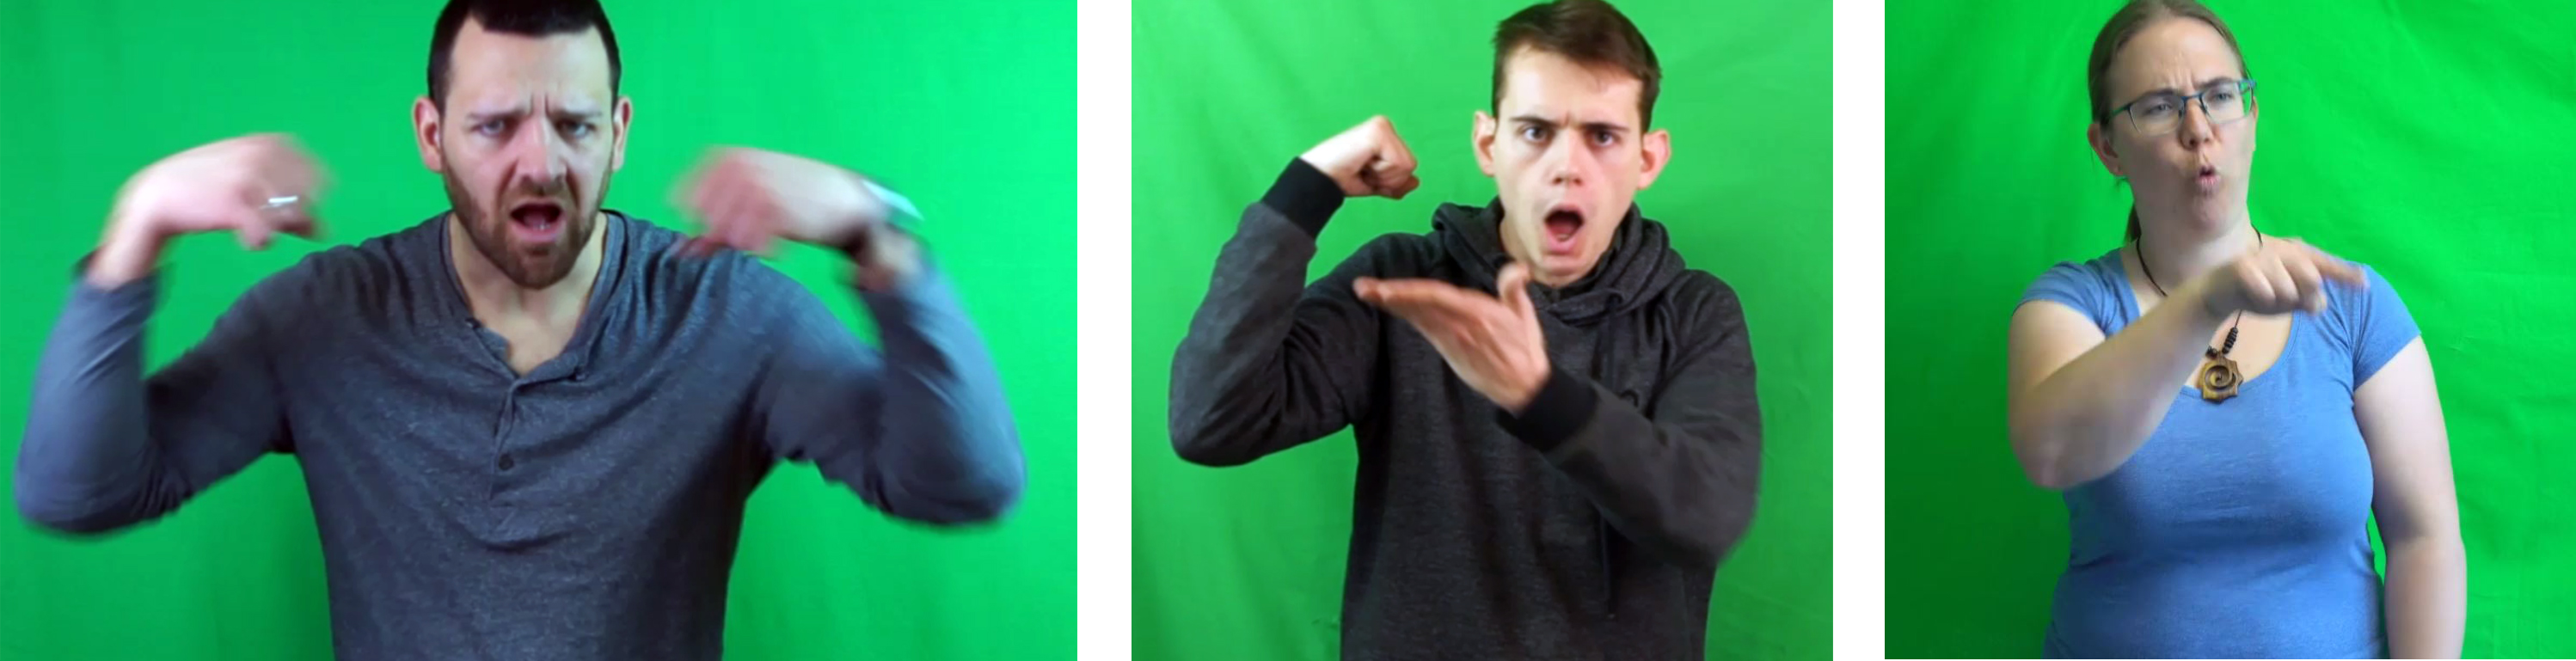
\includegraphics[width=1.0\textwidth]{imperativefacialexpression.jpg}
	\caption{The non-manual markings used in imperatives.}
	\label{fig:imperativefacial}
\end{figure} 

In addition, the signs are produced faster and with more force (see also \citealt[341]{happ2014vork}). These staccato-like movements are often accompanied by rhythmically aligned head bows or head pushes (i.\,e., the head, often together with the upper body, is put forward and backward).\footnote{ A similar observation can be made for American Sign Language. Although \citet{brentari2018production} mention that commands are less likely to be accompanied by head nods, their example in video number 6 clearly shows a similar head push.} To be more precise, my observation is that the bows start with the beginning of the articulation of each sign (the initial hold), arrives at its maximum at the stroke/end hold phase of the sign, and finally, in the preparation phase of the next sign, the head/body is in a reclined position again. This is illustrated in Figure \ref{fig:headmoveimp}. The Figure depicts the sentence \textsc{window always open} `Always open the window!' As can be seen, the head is reclined in the preparation phase of the sign \textsc{window} (1) and is bowed forward in the stroke/end hold phase of the sign (2 and 3). At the transition between the signs \textsc{window} and the adverb \textsc{always} (4 and 5), the head is reclined again.  At the stroke of \textsc{always} (6), the head is bowed forward again, reaching its maximum forward position at the end phase of this sign (7). The same pattern repeats on the last sign \textsc{open}. I'll take the strict alignment with each individual sign as an indication that this phenomenon is prosodic in nature (rhythmic, to be more precise). Similar to assigning word stress on each word in a spoken imperative (\textit{CLOse THE WINdow!}), the head bows seem to have an emphatic function.% As opposed to other sign languages, DGS seems to lack a manual imperative sign. 

\begin{figure}[bt]
\centering
	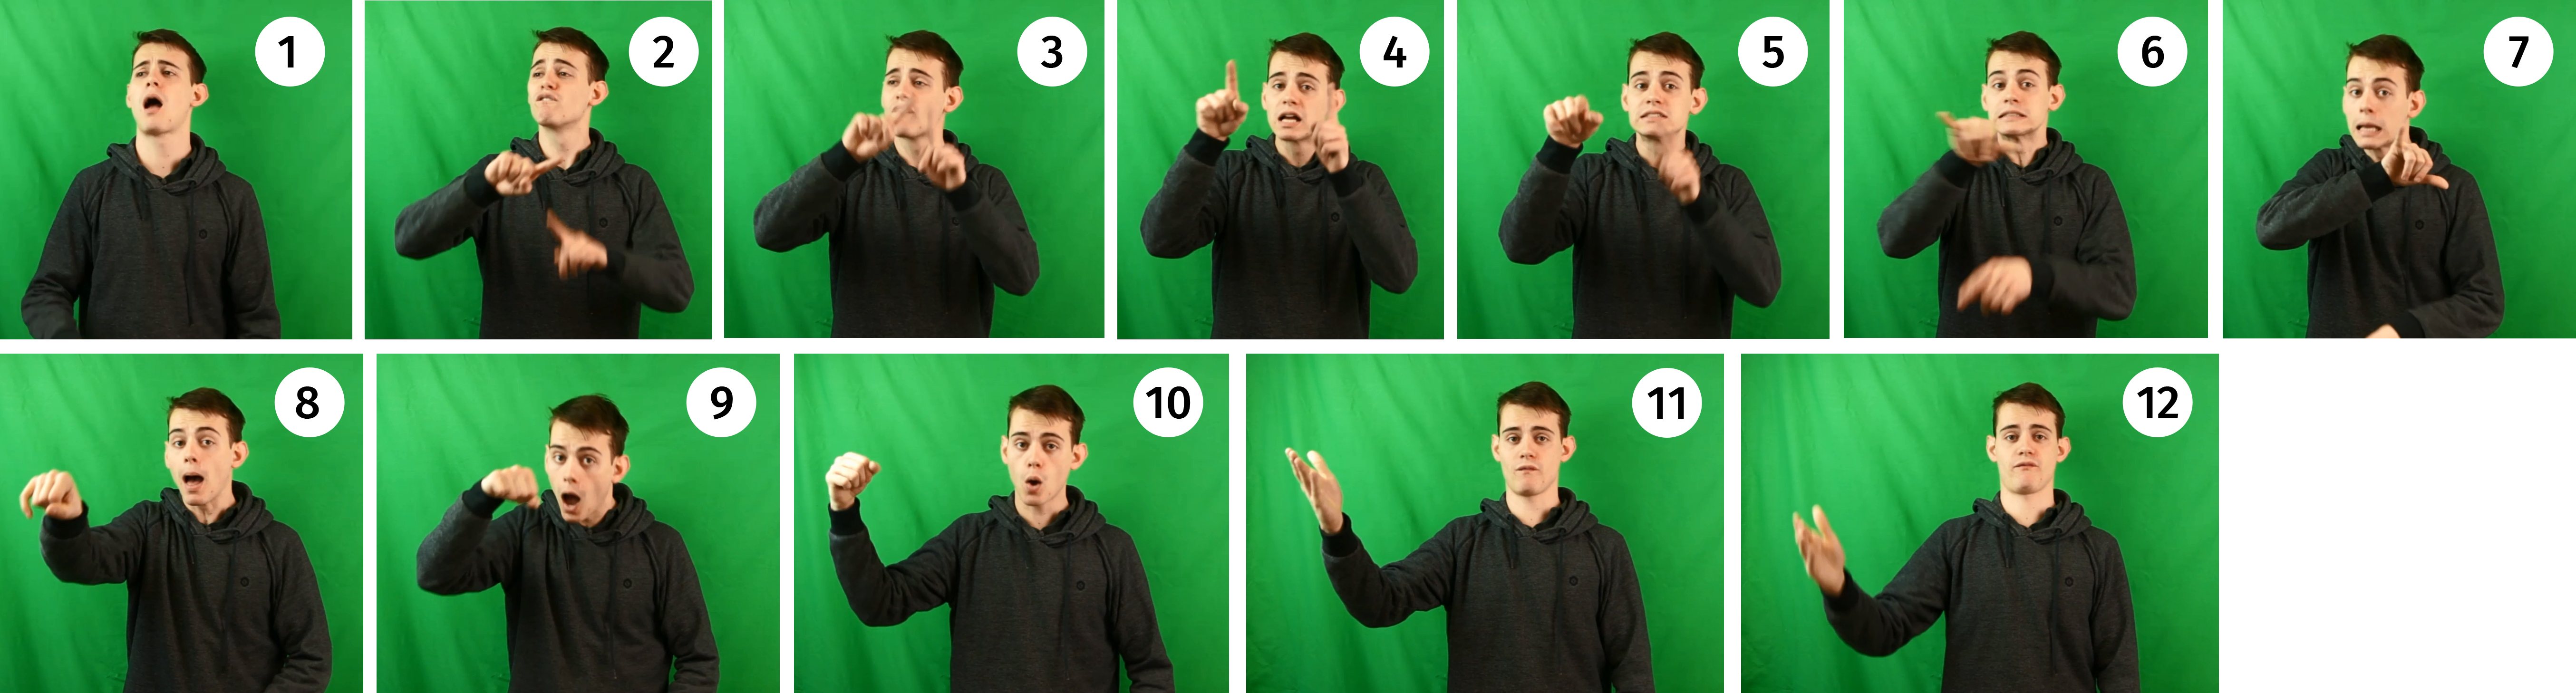
\includegraphics[width=1.0\textwidth]{imperativeheadmovement.jpg}
	\caption{It can often be observed that each sign receives a stress via head or body bows in imperatives.}
	\label{fig:headmoveimp}
\end{figure}

\subsubsection{An imperative sign?}
As the picture shows, sometimes a clause-final imperative sign, similar to the palm-up index sign described for Italian Sign Language in the previous section, can be observed. It remains to be investigated if it is a clear imperative marker or a gesture, but the fact that its position seems to be limited to the clause-final position -- similar to the palm-up gesture in polar interrogatives -- points in the direction of it being a sign. 

\subsubsection{Subject drop}
%Pronoun doubling and the subject position
With imperatives, the addressee of the order can be dropped, i.\,e., there does not have to be an overt pronoun.\footnote{ But note that DGS, in general, allows subject drop.} When such a pronoun is included this is done to give the order more weight. Then, it appears in its usual subject position. Additionally, it can be doubled, just as in interrogatives\is{pronoun!doubling} 

These options are shown in (\ref{imperativedgssimple}). The first of these examples, (\ref{imperativedgssimplea}), shows a typical DGS imperative with the subject dropped. Example (\ref{imperativedgssimpleb}) illustrates that the subject can appear in an imperative. Finally, (\ref{imperativedgssimpled}) shows an instance of pronoun doubling that is, as discussed earlier, possible in polar interrogatives and imperatives in DGS.

\begin{exe}
\ex\label{imperativedgssimple}\begin{xlist} 
\ex \slg[imp]{beer drink}
%
%\ex {\hspace{10pt}imperative}   \\
%{$\overline{\textrm{\textsc{beer drink}}}$}     
\glt `Drink a beer!' \label{imperativedgssimplea}
\ex \slg[imp]{index_2 beer drink}
%
%\ex {\hspace{52pt}imperative}   \\
%{$\overline{\textrm{\textsc{index}\textsubscript{2} \textsc{beer drink}}}$}     
\glt `Drink a beer!' \label{imperativedgssimpleb}
\ex \slg[imp]{index_2 beer drink index_2}
%
%\ex {\hspace{93pt}imperative}   \\
%{$\overline{\textsc{index}\textsubscript{2} \textrm{\textsc{ beer drink} \textsc{index}\textsubscript{2}}}$}     
\glt `Drink a beer!' \label{imperativedgssimpled}
\end{xlist}
\end{exe}

\noindent In contrast to what was described for other sign languages (see the previous section), DGS does not allow proper names in imperatives. Thus, an example like the one in (\ref{imperativesubjectslis}) is not possible.


\begin{exe}
\ex *\slg[imp]{tobias beer drink}
%\ex {\hspace{95pt}imp}   \\
%{*$\overline{\textrm{\textsc{tobias drink beer}}}$}     
\glt \textcolor{white}{*}`Tobias, drink a beer!' \label{imperativesubjectslis}
\end{exe}

\noindent What is, in contrast, possible is to have a quantified DP in an imperative sentence (\ref{quantifieddpimp}). The position of the subject DP is, as the examples show, variable. It can either occur after a temporal adverb (that are usually found in clause-initial positions) (\ref{quantifieddpimpa}) or preceding it (\ref{quantifieddpimpb}). In the first case, the subject DP \textsc{all soldier} seems to be located in the canonical subject position. In the second case, it may be that it is located in a vocative position (and vocatives are, in general, assumed to be hosted in the highest functional structures observed so far, cf. \citealt{moro2003notes, hill2007vocatives, hill2013vocatives}). However, more research on vocatives in DGS is needed. 

\begin{exe}
\ex\label{quantifieddpimp}\begin{xlist}
\ex \slg[imp]{now all soldier hide}
%
%\ex {\hspace{110pt}imp}   \\
%{$\overline{\textrm{\textsc{now all soldier hide}}}$}     
\glt `All soldiers, hide now!' \label{quantifieddpimpa}
\ex \slg[imp]{all soldier now hide}
%
%\ex {\hspace{110pt}imp}   \\
%{$\overline{\textrm{\textsc{all soldier now hide}}}$}     
\glt `All soldiers, hide now!' \label{quantifieddpimpb}
\end{xlist}
\end{exe}

\subsubsection{The imperative verb}
\noindent Concerning the verb form, DGS behaves in an interesting way as there is no special verb form that is used in imperatives. The only difference between other sentence types might be that the verb can be produced  faster and with more force -- however, this is not only true for the verb, but for all signs in an imperative. This is probably done, for example, to give an order more stress. Verbal signs in imperatives, however, show the same agreement behavior as in other sentence types. 

Thus, verb signs used in imperatives agree at least with the object. This is illustrated on the top in Figure \ref{fig:inflectimp}. The figure shows the imperative \textit{Give him the book!} The signer's gaze is directed at the addressee when signing \textsc{book} and then follows the direction of motion of the verb sign \textsc{give} that starts in a position towards the addressee and ends at the location of the referent to whom the book should be given. Thus, the verb \textsc{give} behaves in imperatives just as in assertions. The use of \textsc{give} in an assertion is shown for the translational equivalent of the sentence \textit{Paul hopes that Otto gives him the book} below the imperative in Figure \ref{fig:inflectimp} (note that verb agreement can also be observed in what normally would be considered as infinitival complements).


\begin{figure}[bt]
\centering
	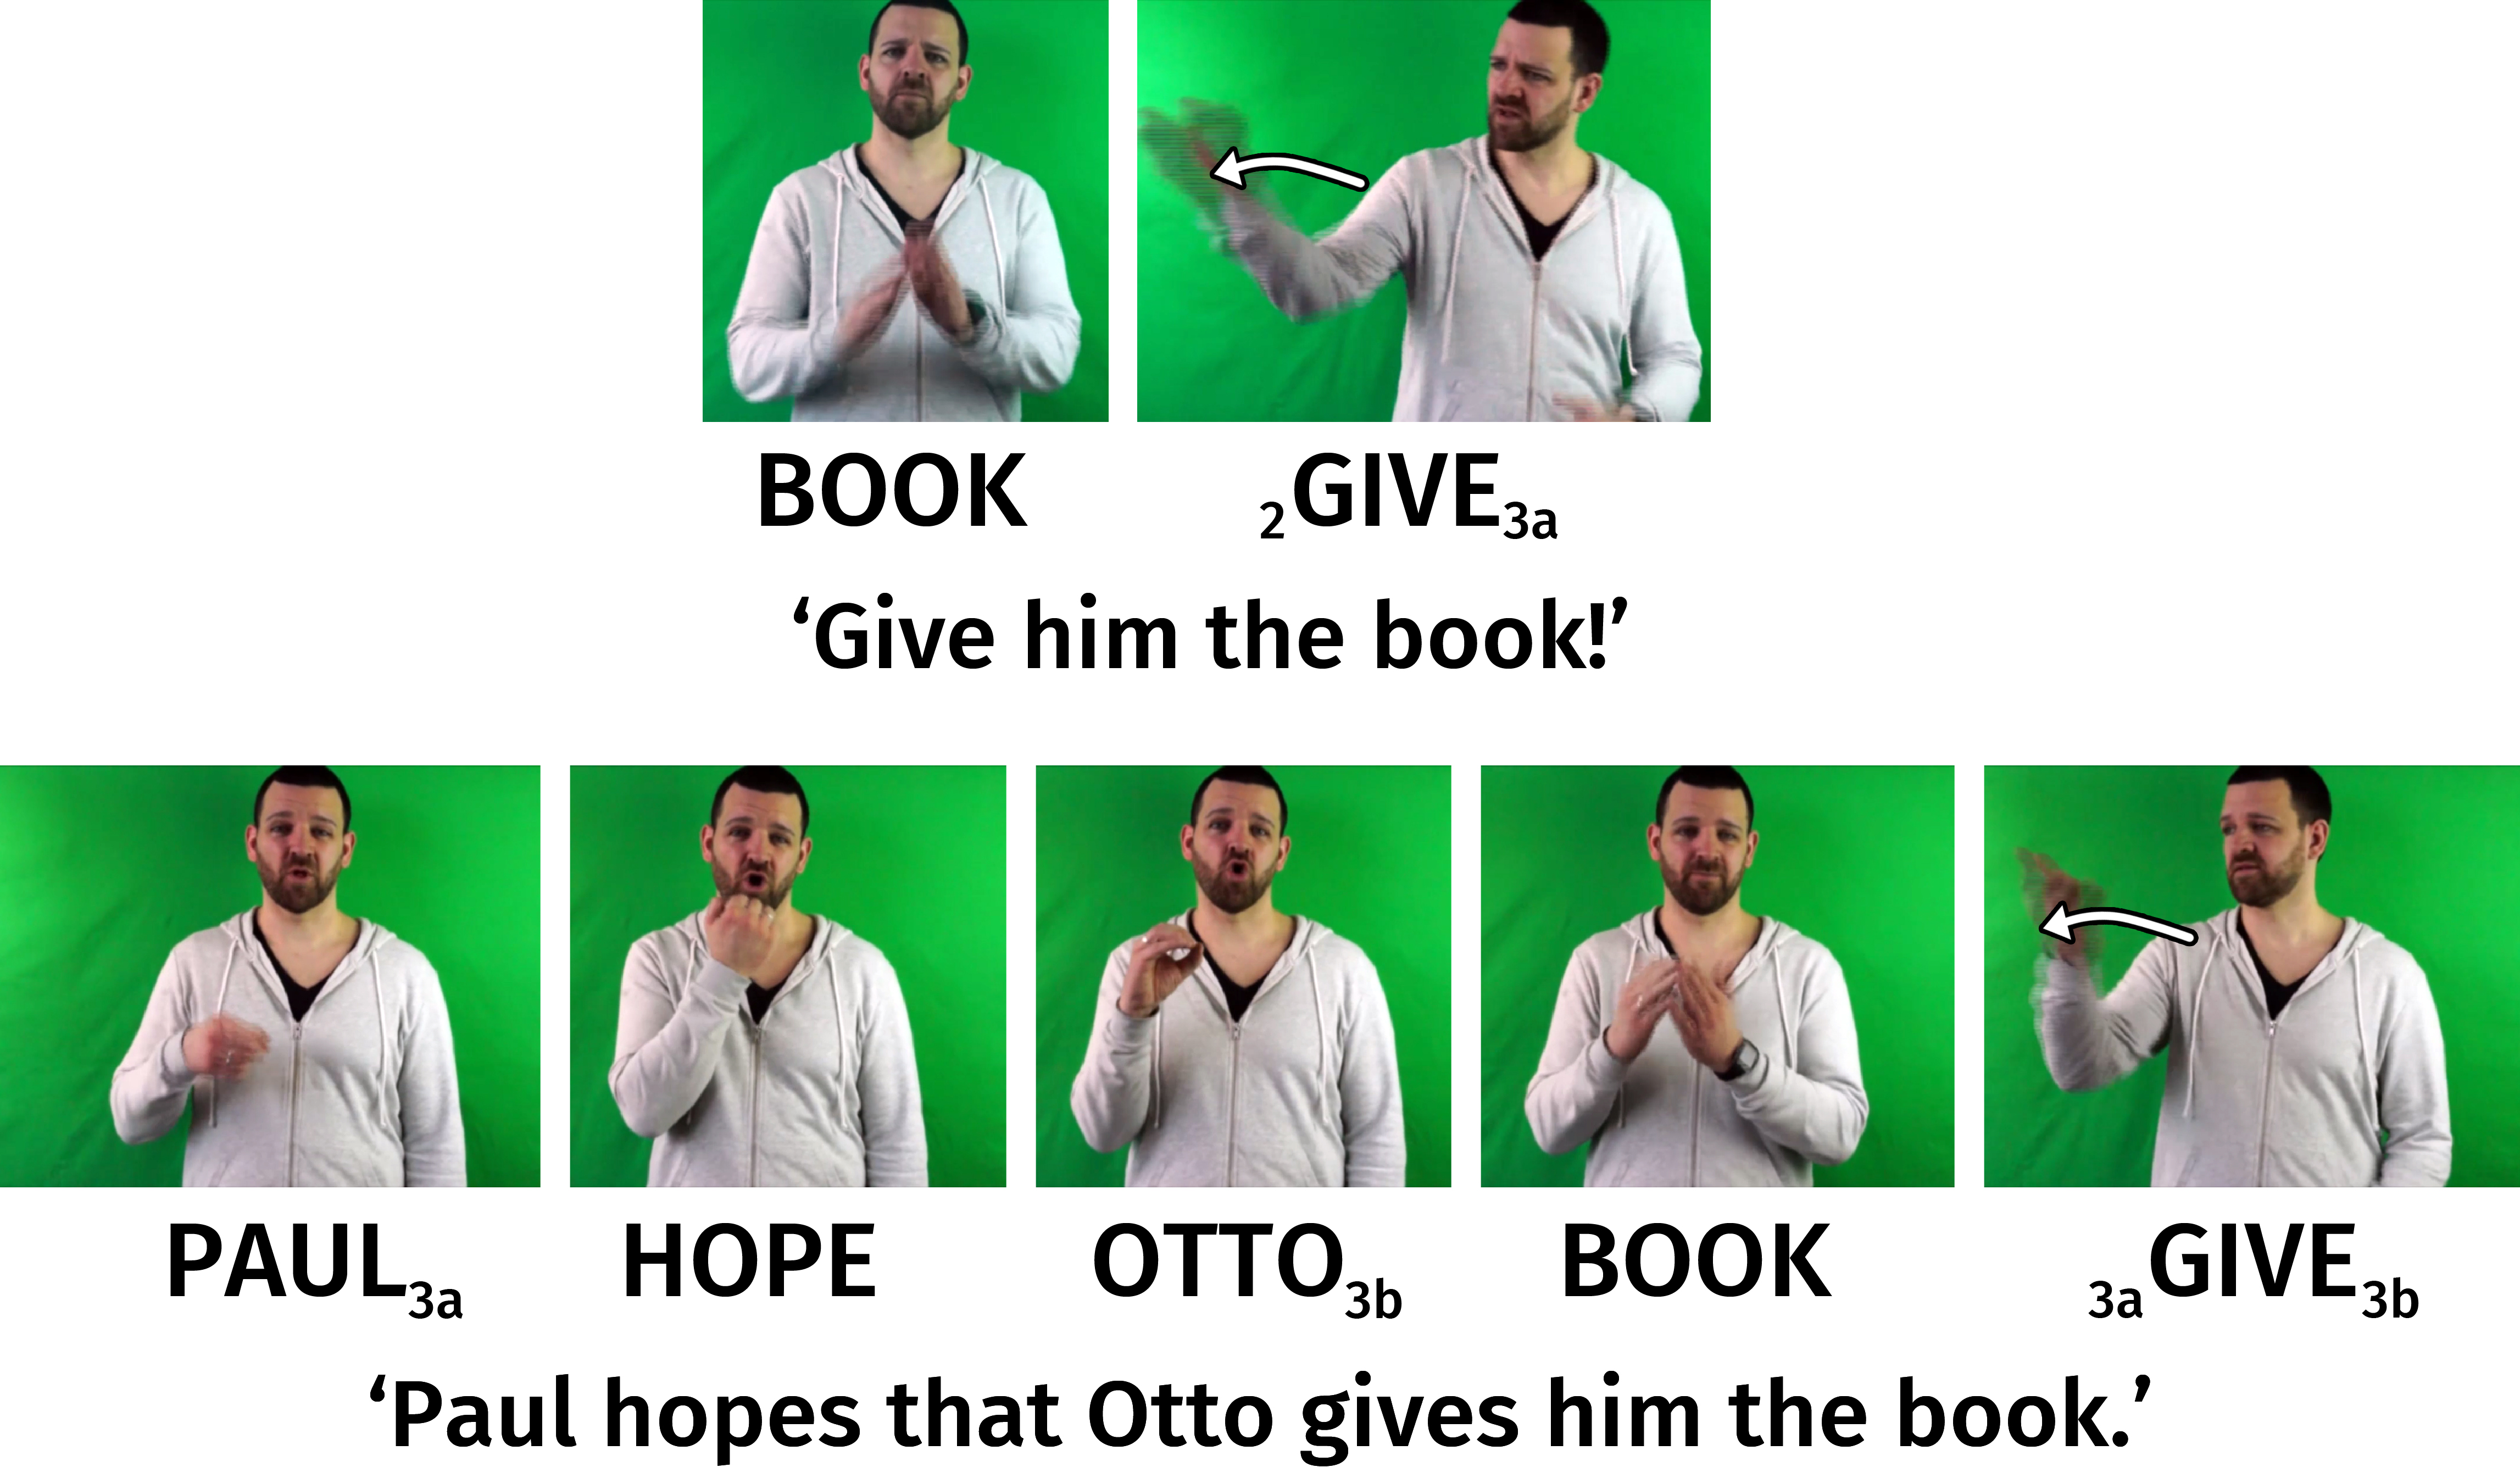
\includegraphics[width=1.0\textwidth]{inflectimp.jpg}
	\caption{Verbal agreement in imperatives does not differ from verbal agreement in other sentence types in DGS.}
	\label{fig:inflectimp}
\end{figure}

That verbs in imperatives show normal agreement should not be too surprising, however. Although it is usually assumed that the functional structure of imperatives is defective, several authors have found evidence that the verb in imperatives still bears its \textit{phi} features (e.\,g., \citealt{henry1995belfast, rupp2002syntax}). Although the imperative verb in present day English, for example, does not show any overt agreement morphology, this was different in Early Modern English as illustrated in the examples in (\ref{impearlymodernenglish}) cited by \citet[25]{rupp2002syntax}.

\begin{exe}
\ex Early Modern English \citep[25]{rupp2002syntax}\label{impearlymodernenglish}\begin{xlist} 
\ex \gll {\textit{O}} {\textit{goddesse}} {\textit{immortal}!} {Be} {\textit{helping}} {\textit{now},} {$[$\dots$]$}  \\
{O} {goddess} {immortal} {be.\textsc{2s.imp}} {helping} {now} {$[$\dots$]$} \\
\trans `O immortal goddess! You be helping now, $[$\dots$]$.' \label{ex:impearlymodernenglisha}
\ex \gll {\textit{Fy}} {\textit{on}} {\textit{yow}!} {goyth} {\textit{hence}} {\textit{Out}} {\textit{of}} {\textit{my}} {\textit{presence}}   \\
{Fie} {on} {you} {go.\textsc{2pl.imp}} {hence} {out} {of} {my} {presence} \\
\trans `Fie on you! Now (you) get out of my sight.' \label{ex:impearlymodernenglishb}
\end{xlist}
\end{exe}

\noindent Early Modern English had, as the example pair shows, a morphological contrast between singular and plural as we still see today in other languages such as German. 

\subsubsection{Negated imperatives}
%Negative imperatives
Before turning to the discussion of negated imperatives in DGS, I will make some general remarks on negation in DGS in the following excursus.\label{negationnegaation}

\is{negation|(}

\begin{digression}{Negation in DGS and the \textit{why-not} test}{}
\noindent Cross-linguistically, sign languages fall into two classes when it comes to negation, as negation can be expressed non-manually or manually. The non-manual strategy usually consist of a head-shake, the manual strategy consists of a manual negator (see \citealt{zeshan2004negation}). DGS is classified as a non-manual dominant language as a head-shake is used as the only marker to express standard negation. According to \citet[55]{pfau2016featural} there are four negation patterns in DGS that are shown in (\ref{pfauneg}). 


\begin{exe}
\ex\label{pfauneg}\begin{xlist} 
\ex \slg{poss_1 brother wine} \slg[hs]{like}
%\ex {} {\hspace{135pt}hs}  \\
%{\textsc{poss\textsubscript{1} brother wine}} {$\overline{\textrm{\textsc{like}}}$} 
\glt `My brother doesn't like wine.' \label{pfaunega}
\ex \slg{poss_1 brother} \slg[hs]{wine like}
%
%\ex {} {\hspace{134pt}hs}  \\
%{\textsc{poss\textsubscript{1} brother}} {$\overline{\textrm{\textsc{wine like}}}$} 
\glt `My brother doesn't like wine.' \label{pfaunegb}
\ex \slg{poss_1 brother wine} \slg[hs]{like neg}
%
%\ex {} {\hspace{160pt}hs}  \\
%{\textsc{poss\textsubscript{1} brother wine}} {$\overline{\textrm{\textsc{like neg}}}$} 
\glt `My brother doesn't like wine.' \label{pfaunegc}
\ex \slg{poss_1 brother} \slg[hs]{wine like neg}
%
%\ex {} {\hspace{160pt}hs}  \\
%{\textsc{poss\textsubscript{1} brother}} {$\overline{\textrm{\textsc{wine like neg}}}$} 
\glt `My brother doesn't like wine.' \label{pfaunegd}


\end{xlist}
\end{exe} 

\noindent Pfau's examples illustrate that the head shake, glossed as `hs', must at least accompany the verb (\ref{pfaunega}), but may spread over the object (\ref{pfaunegb}). For some authors, this pattern is the most neutral form of negation (e.\,g., \citealt{happ2014vork}). When a clause contains a head shake, the manual negator \textsc{neg} (in Pfau's transcription \textsc{not}) may optionally be used, as shown in (\ref{pfaunegc}) and (\ref{pfaunegd}). In all cases, the head shake has to be present at least over the verb (and \textsc{neg} if present).

Interestingly Southern DGS seems to behave differently from what is found in the literature. My consultants unanimously rejected examples with the head shake spreading over the object. The only option left is, thus, that the head shake accompanies the verb, as in example (\ref{pfaunega}). 

A last question concerning negation is the status of the head-shake and \textsc{neg}. Whether they are heads or phrases located in a specifier position can be tested using the \textit{why-not} test \citep{merchant2006no, zeijlstra2015morpho}. A \textit{wh}-element like \textit{why} is phrasal. Therefore it should be disallowed for a head to adjoin \textit{why} (as head-to-phrase adjunction is not possible).  A negative element that is in the specifier of NegP (i.\,e., an XP), in contrast, can adjoin \textit{why}:

\begin{quote}
If the sentential negative marker in a given language is phrasal (an XP, generally adverbial), it will occur in the collocation \textit{why not?}; if it is a head (an X\textdegree , generally clitic-like), it will not. \citep[20]{merchant2006no}
\end{quote}

\noindent The German negator \textit{nicht}, for example, is an XP (depending on the account either located in the specifier of NegP or a vP adjunct). As an XP it is allowed to adjoin with \textit{warum} `why' (\textit{Warum nicht?}). The negative head \textit{nein}, in contrast, cannot adjoin \textit{warum} (*\textit{Warum nein?}). Languages that use negative heads, like Italian, disallow the adjunction of a negative head particle, in Italian the particle \textit{non} to \textit{perchè} `why' (*\textit{Perchè non}). Instead, the word \textit{no} has to be used, i.\,e., an XP (\textit{Perchè no?}). 

Applying the \textit{why-not} test to DGS shows that a head-shake-only strategy is not allowed in the translational equivalent of \textit{why not} (\ref{whynottestdgs}). Instead, the use of the manual negator \textsc{neg} is required, as observed by \citet[56]{pfau2016featural}. These judgments were confirmed by my consultants. 

\begin{exe}
\ex\label{whynottestdgs}\begin{xlist}
\ex\label{ex:modaldoublingneg} *\slg[hs, wh]{why}
%\glll {\hspace{30pt}{}}  {\hspace{27pt}${\hspace{33pt}\underline{\textrm{\quad hn + ec}}}$} \\
%{} {\hspace{1pt}hs/wh}  \\
%{*$\overline{\textrm{\textsc{why}}}$}    
\glt \textcolor{white}{*}`Why not?'

\ex\label{ex:modaldoublingnegb} \textcolor{white}{*}\slg[hs, wh]{why neg}
%\glll {\hspace{30pt}{}}  {\hspace{27pt}${\hspace{33pt}\underline{\textrm{\quad hn + ec}}}$} \\
%{\hspace{25pt}hs/wh}  \\
%{\textcolor{white}{*}$\overline{\textrm{\textsc{why neg}}}$}    
\glt \textcolor{white}{*}`Why not?'
\end{xlist}
\end{exe}


\noindent From this we can conclude that \textsc{neg} is phrasal while the head-shake is a syntactic head (for more details see \citealt{pfau2016featural}).

 

\end{digression}
%%%%%%%%%%%%%%%%%%%%%%%%%%%%%%%%%%%%%%%%%%%%%%%%%%%%%%%%%%
%\clearpage
%%%%%%%%%%%%%%%%%%%%%%%%%%%%%%%%%%%%%%%%%%%%%%%%%%%%%%%%%%

\noindent Negation in negative imperatives clearly differs from negation in declaratives in DGS: while declaratives require the use of a head shake and only optionally allow for the manual negator \textsc{neg}, negative imperatives in DGS are produced via the manual negation marker \textsc{neg} only (the sign \textsc{neg} itself is obligatorily accompanied by a head shake). Negating an imperative via head shake only, in contrast, is not possible, as illustrated by the contrast in (\ref{negimpdgs}).   

\begin{exe}
\ex\label{negimpdgs}\begin{xlist} 
\ex\label{negimpdgsa} \textcolor{white}{*}\slg[imp]{window open \slg[\textup{hs}]{neg}}
\glt \textcolor{white}{*}`Don't open the window!'
\ex *\slg[imp]{window \slg[\textup{hs}]{open}}
\glt \textcolor{white}{*}`Don't open the window!'
\end{xlist}
\end{exe} 

\noindent Alternatively, another negative sign can be used to negate an imperative. This can be, for example, the sign \textsc{not-yet}. %As with \textsc{neg}, these negative signs occupy a clause-final position. 

The observation that regular negation is not allowed in DGS imperatives is in line with the idea that verb movement is blocked in languages in which negation is expressed by a head. This might be the reason why the head-shake in negative imperatives is totally absent on the verb (cf. \ref{negimpdgsa}). While DGS in this respect patterns with other languages that do not allow the regular negator in imperatives, the syntactic analysis of this phenomenon is not straightforward -- at least when it comes to standard analysis of negation in sign languages. The head-shake on the verb in non-imperative sentences was analyzed as an affix. \citet[57]{pfau2016featural}, for example, proposes the two analyses for negation in DGS shown in the trees in (\ref{ex:twoneganalysespfau}) (I slightly adapted the trees). Both model the sentence \textit{My brother doesn't like wine} from the example in (\ref{pfaunega}). The structure in (\ref{ex:twoneganalysespfaua}) allows heads and especially specifiers on both sides while the structure in (\ref{ex:twoneganalysespfaub}) is strictly antisymmetric (for the correct word order, further movement would be required in the antisymmetric structure that is not depicted).

%%%%%%%%%%%%%%%%%%%%%%%%%%%%%%%%%%%%%%%%%%%%%%%%%%%%%%%%%
%\clearpage
%%%%%%%%%%%%%%%%%%%%%%%%%%%%%%%%%%%%%%%%%%%%%%%%%%%%%%%%%

\begin{exe}
\ex\label{ex:twoneganalysespfau}
\begin{multicols}{2}
\begin{xlist}

\ex\label{ex:twoneganalysespfaua}
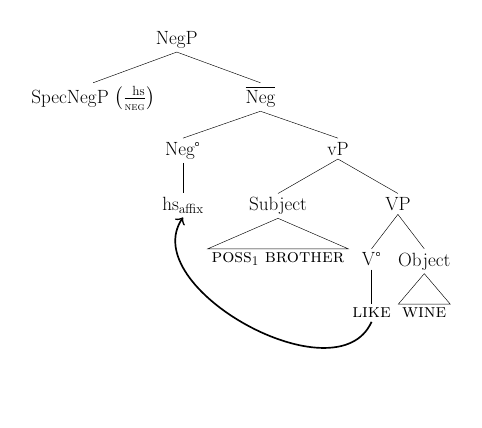
\begin{tikzpicture}[baseline=(current bounding box.north), scale=0.4]
\tikzset{sibling distance=0.1pt,level distance=50pt}
\tikzset{every tree node/.style={align=left,anchor=north}}

\Tree [.{\LARGE NegP} [.{\LARGE SpecNegP {$\left(\frac{\hfill\textrm{hs}}{\textrm{{\normalsize \textsc{neg}}}}\right)$}} ] [.{\LARGE $\overline{\textrm{Neg}}$} [.{\LARGE Neg\textdegree } \node(x){\LARGE hs\textsubscript{affix}}; ] [.{\LARGE vP} [.{\LARGE Subject} \edge[roof];  \node(three){\LARGE \textsc{poss}\textsubscript{1} \textsc{brother}}; ] [.{\LARGE VP} [.{\LARGE V\textdegree } \node(v){\LARGE \textsc{like}}; ] [.{\LARGE Object} \edge[roof];  \node(threet){\LARGE \textsc{wine}}; ] ] ] ] ]



\draw[semithick, <-] (x.south) to [bend right=95] (v.south);
%[.IntP [.SpecIntP ] [.{$\overline{\textrm{Int}}$} [.{Int\textdegree } ] [.FocP [.SpecFocP ] [.{$\overline{\textrm{Foc}}$} [.{Foc\textdegree } ] [.IP \edge[roof]; \node(t){\qquad\qquad}; ] ] ] ] ]

\end{tikzpicture}

\ex \label{ex:twoneganalysespfaub}

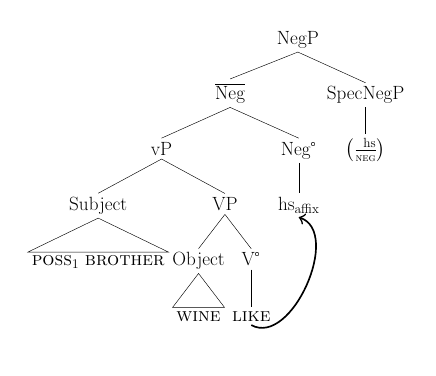
\begin{tikzpicture}[baseline=(current bounding box.north), scale=0.4]
\begin{scope}[xshift=-3cm]
\tikzset{sibling distance=0.1pt,level distance=50pt}
%\tikzset{every tree node/.style={align=left,anchor=north}}

\Tree [.{\LARGE NegP} [.{\LARGE$\overline{\textrm{Neg}}$} [.{\LARGE vP} [.{\LARGE Subject} \edge[roof];  \node(three){\LARGE \textsc{poss}\textsubscript{1} \textsc{brother}}; ] [.{\LARGE VP} [.{\LARGE Object} \edge[roof];  \node(threet){\LARGE \textsc{wine}}; ] [.{\LARGE V\textdegree } \node(v){\LARGE \textsc{like}}; ] ] ] [.{\LARGE Neg\textdegree } \node(x){\LARGE hs\textsubscript{affix}}; ] ] [.{\LARGE SpecNegP} {\LARGE $\left(\frac{\hfill\textrm{hs}}{\textrm{{\normalsize \textsc{neg}}}}\right)$} ] ]

\draw[semithick, <-] (x.south) to [bend right=-95] (v.south);
%[.IntP [.SpecIntP ] [.{$\overline{\textrm{Int}}$} [.{Int\textdegree } ] [.FocP [.SpecFocP ] [.{$\overline{\textrm{Foc}}$} [.{Foc\textdegree } ] [.IP \edge[roof]; \node(t){\qquad\qquad}; ] ] ] ] ]
\end{scope}
\end{tikzpicture}



\end{xlist}
\end{multicols}
\end{exe}


\noindent However, if we analyze the head shake as an affix, we would expect verb movement in imperatives to not be blocked. Instead, it should be possible for the affixed verb to move to the CP projection hosting the imperative feature (let's say to the head of an ImpP). Alternatively, one could propose that the verb in head-shake-only negation does not move to Neg\textdegree\ at all, but that it is activated by a covert element. The head shake then spreads over its c-command domain (that the head shake does not spread over the object in Southern DGS could be explained either by the fact that NegP is lower in the structure or that the object obligatorily moves into a higher structural position). This is in line with \citet{zeijlstra2004sentential} proposals that languages that do not allow regular negation of imperatives are languages with a base-generated Neg\textdegree . If this is on the right track, the mechanism behind the head shake would work just as described for other cases of non-manuals previously mentioned. Concerning negated imperatives, this would mean that verb movement to Imp\textdegree\ is blocked by a covert element in Neg\textdegree . 


Taken together, I assume that with imperatives, feature checking occurs with a high CP category. This is probably done in a functional projection ImpP. As with the other sentence types, this can be modeled either by assuming a right-headed Imp\textdegree , triggering the non-manual markers or by assuming a left-branching SpecImpP to which the lexical material moves to check the features. Both accounts are in line with the fact that the palm-up index sign is found in a clause-final position. However, more research on DGS imperatives is clearly needed.

\is{negation|)}
\is{imperatives|)}


\section{Optatives}\label{opt}
\subsection{General overview}
\is{optative|(}
Optatives express wishes. They are regarded as a minor sentence type as not many languages have grammaticalized means of expressing optative mood. English often uses modal verbs (e.\,g., \textit{May the force be with you!}) or conditional constructions with \textit{only} (e.\,g., \textit{If only I had won the lottery!}). In German, optatives are often expressed using the subjunctive mood as shown in example (\ref{ex:optativegermansubjunctive}). 


\begin{exe}
\ex German \\ \gll {\textit{Hätte}} {\textit{Paul}} {\textit{doch}} {\textit{eine}} {\textit{Freundin!}}   \\
{have.\textsc{subj}} {Paul} {modal particle} {a} {girlfriend}\\
\trans `If only Paul had a girlfriend!' \label{ex:optativegermansubjunctive}
\end{exe}

\noindent While English and German use means to express optative mood that also serve different functions, there are languages that mark this category in the inflectional domain of the verb. This was, for example, the case in Ancient Greek. An example taken from \citet[216]{palmer2001mood} is given in (\ref{ex:palmer}).

\begin{exe}
\ex Greek \citep[216]{palmer2001mood} \\ \gll {\textit{ei}} {\textit{gár}} {\textit{genoíme\textlengthmark n}} {\textit{téknon,}} {\textit{antí}} {\textit{soú}} {\textit{nekrós}}          \\
{oh} {that} {become.1\textsc{sg.aor.opt}} {son} {instead.of} {you} {corpse}  \\
\trans `Oh that I might be a corpse, my child, instead of you!' \label{ex:palmer}
\end{exe}

\noindent Thus, there is cross-linguistic variation as to whether a language has grammaticalized means to express optative mood or not.

\subsection{Optatives in DGS}
The literature on optatives in DGS is extremely scarce. \citet[366]{happ2014vork} mention, without going into detail, that optative can be expressed non-manually only. Concerning my own data, signers fall into two classes. While some signers indeed allow for a non-manual-only expression of optatives, the majority of signers use a performative strategy without any non-manual markers.

The non-manual expression of optatives used by some signers is mainly achieved with narrowed eyes. Additionally, the head is tilted backwards. Again, the non-manuals have their intensity peak towards the end of the clause. In stark contrast to imperatives, the sign duration in optatives is slowed down.  An example of the non-manual only strategy is given in Figure \ref{optativesnonmanuals}.  

\begin{figure}[bt]
\centering
	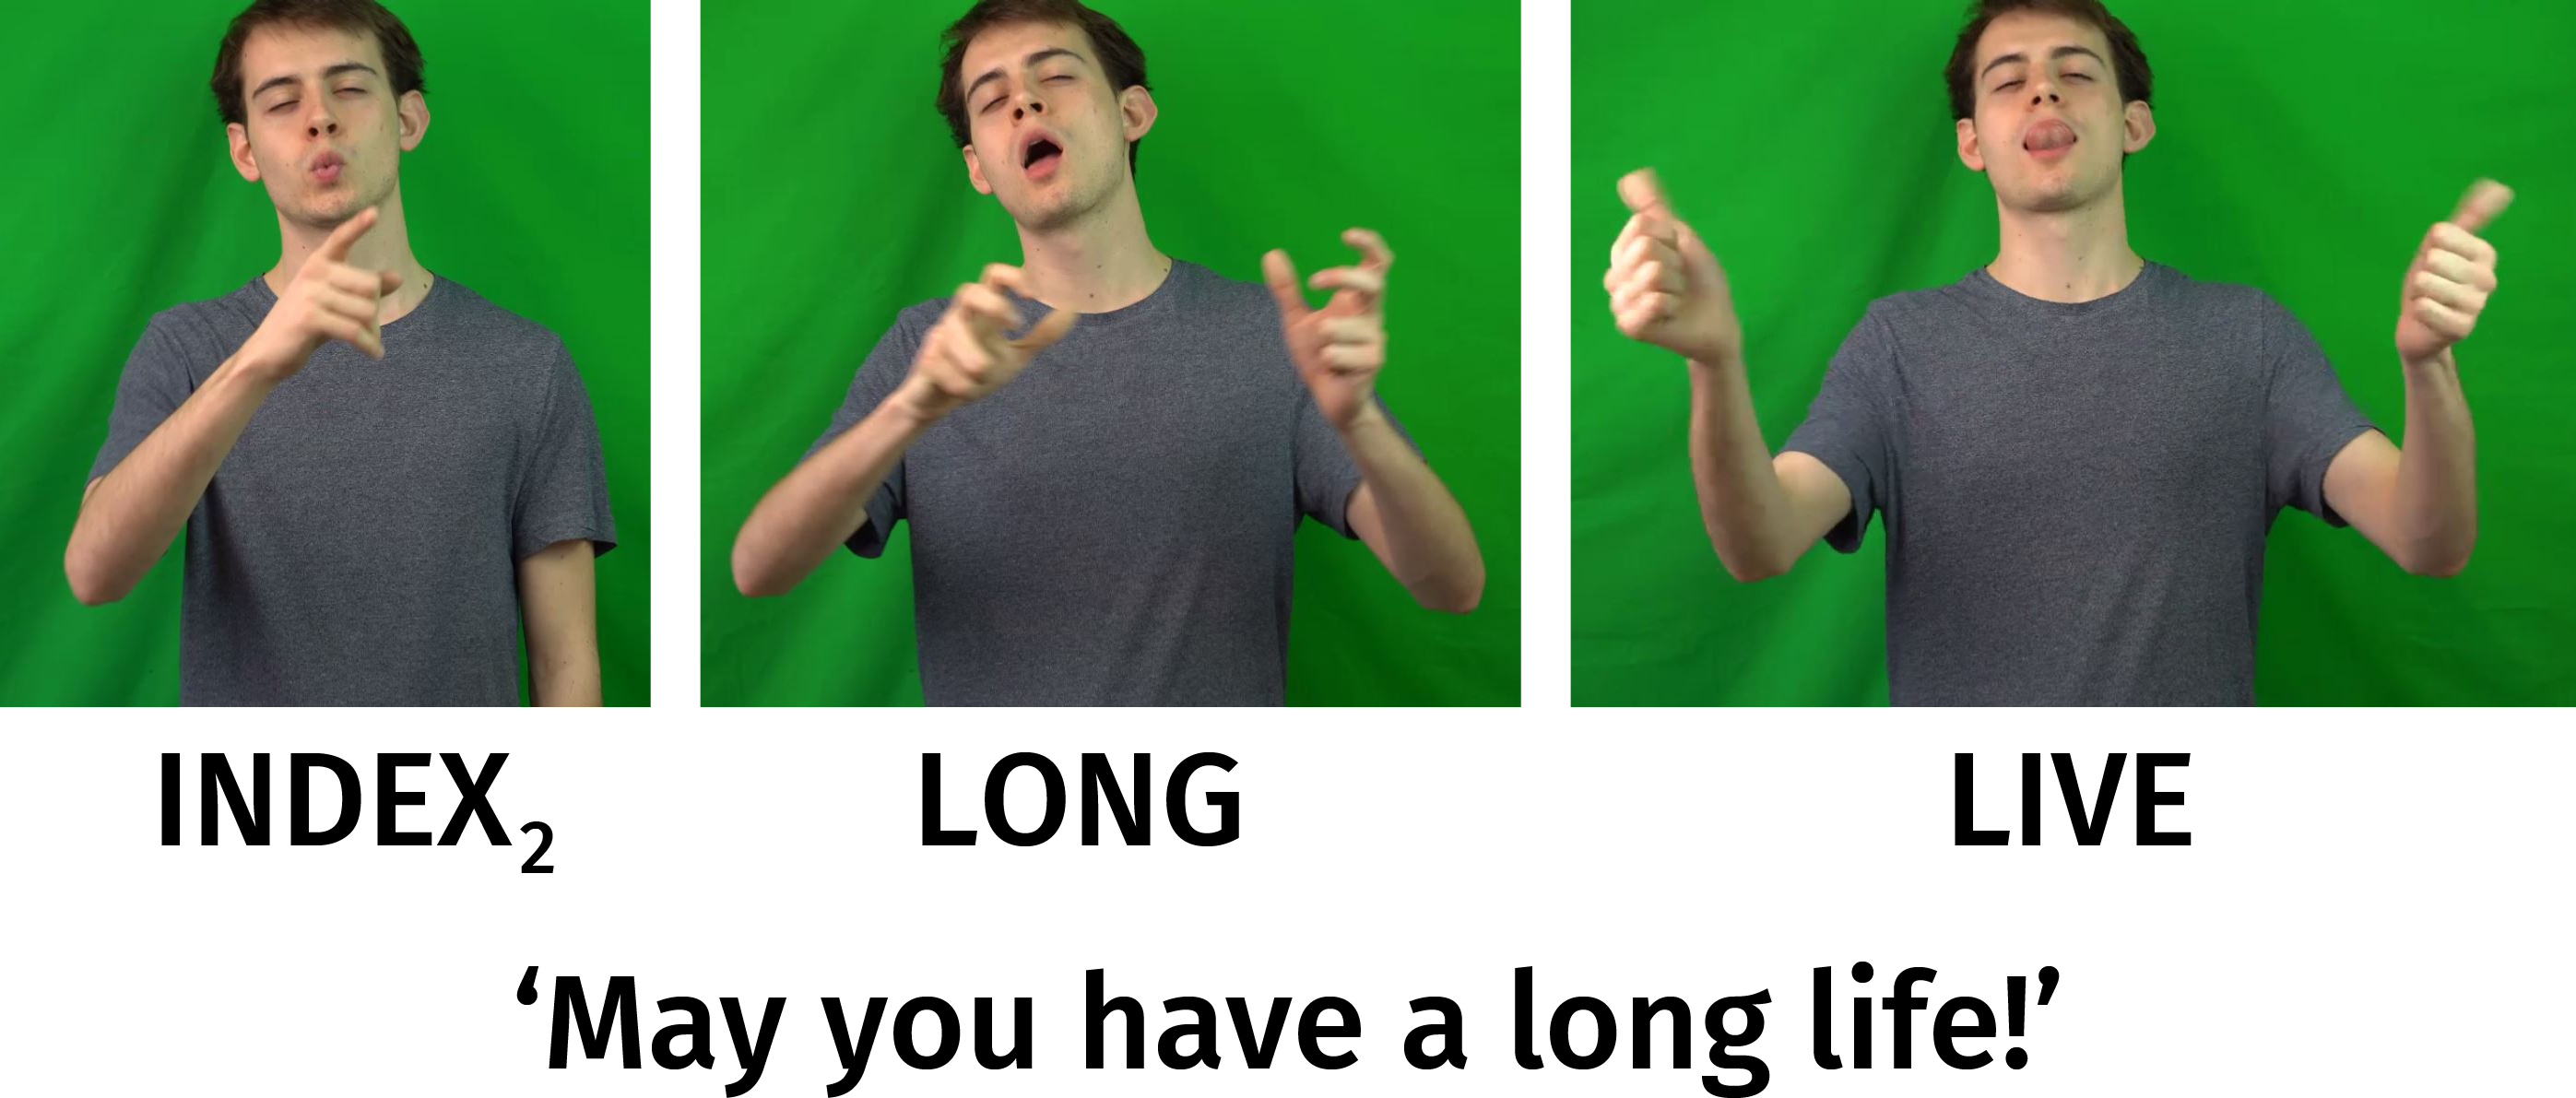
\includegraphics[width=1.0\textwidth]{optative.jpg}
	\caption{The main non-manual marker of optative mood consists of narrowed eyes.}
	\label{optativesnonmanuals}
\end{figure}

Most signers only allow for a strategy using performative verbs like \textsc{wish} or \textsc{like}, i.\,e., as there seems to be no grammaticalized way expressing them, they do not need to receive non-manual markings. This is shown in (\ref{ex:optativedgs}).

\begin{exe}

\ex{\textsc{index\textsubscript{1} wish paul there girlfriend}} 
\glt `If Paul only had a girlfriend!/I wish Paul had a girlfriend!' \label{ex:optativedgs}

\end{exe} 

\noindent It is yet unclear where this variation comes from and why some signers seem to have a grammaticalized form of an optative while others do not.

\is{optative|)}

\section{Summary and conclusion}
The goal of this chapter was to present the expression of left-peripheral categories in DGS, i.\,e., the higher CP domain, and to test the main hypothesis that categories with high scope are expressed using physically high articulators (see Section \ref{hypotheses} for a detailed description of the hypotheses put to test in this book). Taken together, all high CP categories find non-manual expression with the highest possible articulator, namely with the eyebrows/the eyes (or the eyebrows/eyes plus another articulator), as predicted. 

For topics, I have shown, following the literature on different kinds of topics in American Sign Language, that DGS exhibits at least two different types, namely those that are probably moved into left-peripheral position (i.\,e., integrated topics) and those that are base-generated in a slightly higher structural position (i.\,e., non-integrated topics). The two topic types receive different non-manual markings with the main articulators being the eyebrows in both cases. In line with previous research (e.\,g., \citealt{benincapol2004topic}), I have argued that non-integrated topics are structurally higher than integrated topics. The reflex of this can be seen in DGS by the fact that integrated topics have to follow non-integrated topics.

Focus in DGS is also marked non-manually. While information focus is usually not marked at all, sometimes wide-opened eyes and a short eyebrow raise can be observed, the marking of contrastive focus is subject to dialectal variation. While the signers from Baden-Württemberg tilt their heads backwards and raise their eyebrows, signers from Bavaria showed the exact opposite pattern as they put their heads and eyebrows down. Both patterns are in line with the bodily-mapping hypothesis as contrastive focus, as a structurally very high category is marked with the eyebrows. 

Concerning the encoding of sentence types I have shown that while declaratives are unmarked, polar interrogatives, constituent interrogatives, imperatives, as well as other, minor sentence types are marked non-manually with the eyebrows, with the non-manuals spreading over the whole clause. A general pattern that can be found in all sentence types is that the intensity peak of the non-manuals is towards the end of the clause. For polar interrogatives I have shown that their main marker is an eyebrow raise. Additionally, the head is put forward to indicate that the signer expects a response from the addressee and the head is tilted sideways. Evidence for the claim that putting the head forwards encodes the signer's expectation of a response came from the fact that it is absent in rhetorical questions. For the sideays head tilt I claimed that its function is to indicate the signer's epistemic commitment. Evidence for this claim came from the fact that the sidewards tilt is absent in inclination questions of the sort \textit{Can you pass me the salt?} in which the signer is not insecure about the proposition expressed. I will present more evidence for this claim in Section \ref{perhapsmoodirrealis} in the next chapter (see page \pageref{perhapsmoodirrealis}). Taken together, the idea is that three non-manual markers are used in polar questions to express three different functions: speech-act indication (raised eyebrows), expecting a response (head forward), and epistemic commitment (head tilt sideways). 

Following the suggestions that the palm-up gesture \textsc{p-ug} is located in the head of the InterP \citep{aboh2010sa} and that pronoun doubles are located in the head of a focus phrase \citep{de1999phrase, sandler2006sign}, I argued that a model with a right-headed InterP and a right-headed SpecFocP is more economic as it requires less movement steps to derive the fact that \textsc{p-ug} has to follow (and hence cannot precede) a focus double in polar interrogatives. However, other modeling possibilities do exists, as discussed.

As with polar interrogatives the non-manuals of constituent interrogatives spread over the whole clause and have their intensity peak towards the end of the clause. Instead of raising the eyebrows, the brows are lowered in this sentence type. Similar to polar interrogatives, the head is put forward to indicate that the signer is expecting a response. As was described for other sign languages, \textit{wh}-elements naturally occur in a clause-final position, although the pattern is more complex. While the unmarked position of simple \textit{wh}-phrases, like \textsc{what} or \textsc{who}, and \textit{wh}-phrases contained in a PP, like \textsc{with who}, is clause-final, complex \textit{wh}-phrases, like \textsc{which computer}, are usually found clause-initially. Another difference between simple and PP-\textit{wh}-phrases on the one hand and complex \textit{wh}-phrases on the other hand that was found was that the first two can undergo doubling, however this is not true for the latter. These differences were explained by assuming that the first two are syntactic operators while the latter are not. The distributional facts of the \textit{wh}-phrases were captured by a Split-CP model with different landing sites for different kinds of \textit{wh}-phrases. As with polar interrogatives I proposed two modeling possibilities, one allowing heads and specifiers on both sides of the tree and one antisymmetric model. Again, the non-antisymmetric model had the advantage that less movement steps are required to derive the correct surface order.

The discussion of questions was concluded by short notes on some other types of interrogatives and their encoding in DGS. I have briefly discussed alternative, degree, tag, suggestive, and rhetorical questions. While the non-manuals in alternative, degree, and tag questions are not different from polar interrogatives, a difference between information-seeking constituent questions and suggestive questions was described and it was shown that the non-manuals of rhetorical questions depend on the answer to be reconstructed. For degree questions it was shown that this question type, which often takes the form of a \textit{wh}-question in spoken languages, has its own encoding strategy in DGS which is strikingly different from \textit{wh}-questions, thus suggesting that it constitutes a type in its own right. 

Similar to the non-manuals encoding other sentence types, the non-manuals used in imperatives are furrowed brows which have their intensity peak towards the end of the clause. Similar to the palm-up gesture used in questions, a similar imperative sign that is occasionally used in a clause-final position was reported. DGS, as was shown, allows for subject drop in imperatives and proper names are generally disallowed in this sentence type. Concerning negation I have discussed that DGS follows a cross-linguistic trend in that negation in imperatives differs from negation in other sentence types. To be more precise, the manual negator \textsc{neg}, a phrasal element, has to be used in negative imperatives instead of the head-shake which has the status of a syntactic head. This observation is in line with the idea that movement of the verb to a higher CP projection hosting an imperative feature is blocked in the presence of an intervening Neg\textdegree .

The last sentence type I have briefly discussed were optatives. For this sentence type, I have shown that while most signers use performative verbs like \textsc{wish} or \textsc{like} some signers use a non-manual-only strategy. 

Taken together, the data presented in this chapter supports the idea that all categories above tense find non-manual expression in DGS and is in line with the \is{bodily-mapping hypothesis}bodily-mapping hypothesis, as the highest CP functions, including topic and focus marking as well as sentence-type encoding, make use of the highest articulators available, namely the eyebrows. Note that the present chapter did not discuss the status of FinP which would be predicted to active upper-face non-manuals. I hope that I can address the expression of FinP elements in future research. The goal of the next chapter is to shed light on the categories in the lower part of the CP and the IP-internal categories and their expression.



\chapter{The lower CP and the IP area}\label{ipsystem}
As discussed in the previous chapter, all high CP categories, i.e., speech-act-indicating expressions as well as topic and focus marking, are expressed non-manually (with the eyebrows/eyes) in DGS. These observations are in line with the \is{bodily-mapping hypothesis}bodily-mapping hypothesis by \citet{bross2017scope} discussed in Section \ref{hypotheses}. In this chapter I will discuss the organization of the lower portion of the CP and the organization of the IP system in DGS. In general, I will follow \citeauthor{cinque1999adverbs}'s (\citeyear{cinque1999adverbs, cinque2006restructuring}) insights into the order of clausal functional projections, with some modifications (see Section \ref{introcinque} and \ref{anoteonmodality}). I identify the lower portion of the CP with the \is{speaker-oriented adverbs}(speaker-oriented) categories above tense and the IP with the categories below tense and above Voice in Cinque's system. The guiding hypothesis will be, again, the idea that all categories above tense find their expression with high body parts, i.e., non-manually by way of layering. In line with previous observations \citep{bross2017scope}, categories below tense are expressed manually, either by a left-to-right-concatenation strategy (pre-verbally) or, at the lower end of the categories above the VoiceP, by a right-to-left-concatenation strategy (post-verbally). While this is rather obvious for manual adverbs, the exact position for modal verbs will turn out to be more complicated. 

Additionally, \citeauthor{bross2017scope}'s (\citeyear{bross2017scope}) not-at-issue hierarchy stating that the categories above tense mainly express non-truth-conditional meaning will be discussed (see Section \ref{atnotissue}). The higher categories, i.e., those above tense, that are examined in this chapter are encoded either non-manually only or by combining non-manual markings with manual signs that appear clause-initially. I will argue that these non-manuals are reflections of the respective functional heads and that the non-manuals contribute not-at-issue meanings while the manual signs are used for at-issue information. One crucial finding concerning the categories above tense presented in this chapter is the spreading behavior of the non-manuals. While the non-manuals of the higher CP area discussed in the previous chapter had their intensity peak towards the end of the clause, the non-manuals that are used with or without a manual adverb show the opposite behavior: the intensity of the non-manuals is highest at the beginning of the clause and diminishes towards the end. Under the widespread assumption that the greatest intensity of the non-manuals marks their position of origin, i.e., the location of the head that triggers the non-manuals (cf. \citealt{bahan1996, petronio1997}; \citealt[43--45]{neidle2000syntax}; \citealt[311--312]{sandler2006sign}), I will argue that most of the higher heads discussed in this section are left-headed (as opposed to the higher CP heads that can be taken to be right-headed). Finally, the categories below tense (and above Voice) only find their expression manually, first using a left-to-right concatenation strategy, and finally switching to a right-to-left concatenation strategy in the lower portion of the IP. The categories below Cinque's Voice projection will be discussed in the next chapter. %Bahan 1996; Petronio \& Lillo-Martin 1997; Neidle et al. 2000:43--45; Sandler \& Lillo-Martin 2006:311--312)

Readers familiar with the literature on the expression of aspect in sign languages will notice that some of my claims seem to be controversial. It will, for example, be claimed that durative or habitual aspect are expressed manually in DGS and not by a modification of the verb sign (as, for example, discussed in \citealt{rathmann2005event} for \is{American Sign Language}American Sign Language or in \citealt{happ2014vork}  for DGS). I will briefly expound the problems in the relevant sections and discuss them again in the next chapter. 

\section{Introduction: the Cinquean hierarchy}\label{introcinque}
Since the early days of Minimalist Syntax the question of how to model adverbial modification has been a controversial topic. This controversy can be illustrated by a widely cited endnote (n. 22) by \citet[382]{chomsky1995categories} who notes that ``we still have no good phrase structure theory for such simple matters as $[$\dots $]$ adjuncts of many different types''. The debate has mainly revolved around two different modeling possibilities: according to traditional accounts, adverbs are adjuncts (e.g., \citealt{travis1988syntax, potsdam1999syntax, ernst2004principles, vanvalin2005exploring}) and according to Cartographic accounts \citep{cinque1999adverbs, cinque2006restructuring}, adverbs are specifiers of strictly ordered functional projections. 

Traditionally, adverbs were, as noted, considered to be adjuncts. In this view, the adjunction to a category consequently leads to the expansion of this category. Analyzing adverbs as adjuncts seems reasonable since a sentence containing an adverb is still grammatical without the respective adverb and the sentence without the adverb does not entail the adverbial relation as one would expect from an argument (cf.  \citealt{hole2015arguments}).  One prediction that the adjunction analysis makes, however, is that the position and order in which adverbs appear in a sentence should be relatively free. Considering the adjunction site of adverbs in a clause, this prediction, at least superficially, turns out to be true, as illustrated in (\ref{adverbpositionadjunkb}) and (\ref{adverbpositionadjunkc}).

\begin{exe} 
\ex \label{adverbpositionadjunk}\begin{xlist} 
%\ex Often, Paul walked alone in the dark. \label{adverbpositionadjunka}
\ex Felicia cleverly avoided getting caught. \label{adverbpositionadjunkb} % Meaning Paul was clever
\ex Felicia avoided cleverly getting caught.\label{adverbpositionadjunkc} % Meaning Paul's behavior was clever
\end{xlist} 
\end{exe}

\noindent The different adverb positions in (\ref{adverbpositionadjunkb}) and (\ref{adverbpositionadjunkc}) make an adjunct analysis plausible as it seems as if the adverb \textit{cleverly} can be adjoined to different positions (leaving a movement analysis aside for the moment).\footnote{ What is not predicted by the adjunction approach and what will be crucial in the later discussion is that the meanings of the adverbs in (\ref{adverbpositionadjunk}) differ slightly as a function of their position.} However, not only the position inside a clause, but also the relative order of adverbs within clauses containing several adverbs should be free according to an adjunct account. 

As famously argued in \citet{cinque1999adverbs}, however, this prediction is not accurate. \citet[5--6]{cinque1999adverbs}, for example, illustrates that the Italian adverbs \textit{mica} `not', \textit{più} `any longer', and \textit{sempre} `always' cannot be ordered freely, but exhibit rigid ordering restrictions. First, consider the order of \textit{mica} and \textit{più}:

\begin{exe} 
\ex Italian \citep[5]{cinque1999adverbs} \label{cinqueonadverborderingbiga} \begin{xlist} 
\ex \gll {\textit{Non}} {\textit{hanno}} {\textit{chiamato}} {mica} {più,} {\textit{da}} {\textit{allora}.}  \\
{Not} {have} {telephoned} {not} {any-longer} {since} {then}\\
\trans `They haven't telephoned any longer, since then.' \label{cinqueonadverborderingaa}
\ex \gll \llap{$^*$}{\textit{Non}} {\textit{hanno}} {\textit{chiamato}} {più} {mica,} {\textit{da}} {\textit{allora}.}  \\
{Not} {have} {telephoned} {any-longer} {not} {since} {then}\\
\trans `They haven't telephoned any longer, since then.' \label{cinqueonadverborderingab}
\end{xlist} 
\end{exe}

\noindent As the examples (\ref{cinqueonadverborderingaa}) and (\ref{cinqueonadverborderingab}) show, the negative adverb \textit{mica} has to precede \textit{più} in Italian. For the adverbs \textit{più} and \textit{sempre}, we find similar ordering restrictions, as illustrated by the examples in (\ref{cinqueonadverborderingba}) and (\ref{cinqueonadverborderingbb}).

\begin{exe} 
\ex Italian \citep[6]{cinque1999adverbs}\label{cinqueonadverborderingbigb} \begin{xlist} 
\ex \gll {\textit{Da}} {\textit{allora},} {\textit{non}} {\textit{ha}} {più} {sempre} {\textit{vinto}.}  \\
{Since} {then} {not} {have} {any-longer} {always} {won}\\
\trans `Since then, he has no longer always won.' \label{cinqueonadverborderingba}
\ex \gll \llap{$^*$}{\textit{Da}} {\textit{allora},} {\textit{non}} {\textit{ha}} {sempre} {più} {\textit{vinto}.}  \\
{Since} {then} {not} {have} {always} {any-longer} {won}\\
\trans `Since then, he has no longer always won.'  \label{cinqueonadverborderingbb}
\end{xlist} 
\end{exe}

\noindent So far, the examples in (\ref{cinqueonadverborderingbiga}) and (\ref{cinqueonadverborderingbigb}) have given us two orders, namely \textit{mica} $>$ \textit{più} and \textit{più} $>$ \textit{sempre}. \is{transitivity (method)}By transitivity, we can now conclude that if \textit{mica} has to precede \textit{più} and \textit{più} itself precedes \textit{sempre}, then \textit{mica} should also precede \textit{sempre} when combining the two (see the detailed description of the transitivity method in Section \ref{cartographicenterprise}). This, indeed, is the correct prediction as shown in (\ref{cinqueonadverborderingbigc}).

\begin{exe} 
\ex Italian \citep[6]{cinque1999adverbs}\label{cinqueonadverborderingbigc} \begin{xlist} 
\ex \gll {\textit{Gianni}} {\textit{non}} {\textit{ha}} {mica} {sempre} {\textit{vinto}.}  \\
{Gianni} {not} {has} {not} {always} {won} \\
\trans `Gianni hasn't always won.' \label{cinqueonadverborderingca}
\ex \gll \llap{$^*$}{\textit{Gianni}} {\textit{non}} {\textit{ha}} {sempre} {mica} {\textit{vinto}.}  \\
{Gianni} {not} {has} {always} {not} {won} \\
\trans `Gianni hasn't always won.'  \label{cinqueonadverborderingcb}
\end{xlist} 
\end{exe}

\noindent As the Cinquean examples above have shown, adverbs in Italian are rigidly ordered (unless an additional reordering, for example, for focusing purposes, has taken place). So far, we arrive at the order illustrated in (\ref{bsp:rigidorderone}).


\begin{exe}
\ex\label{bsp:rigidorderone} 
\textit{mica} $>$ \textit{più} $>$ \textit{sempre}
\end{exe}

\noindent By a pairwise comparison of adverb orderings in Italian, French, and English and finally, by drawing on data from a number of other, unrelated languages, \citet{cinque1999adverbs} developed a presumably universal hierarchy of adverb categories known as the `Cinquean hierarchy', the `universal hierarchy of clausal functional projections', the `universal scope order of clausal categories', or `hierarchy of inflectional categories'. A preliminary version of this hierarchy, based on \citet[106]{cinque1999adverbs} is given in (\ref{bsp:hierarchyoneafafaf}).

\begin{exe}
\ex\label{bsp:hierarchyoneafafaf} 
{\small $[$\textit{frankly} Mood\textsubscript{speech act} \\
\textcolor{white}{nn}$[$\textit{fortunately} Mood\textsubscript{evaluative} \\
\textcolor{white}{nnn}$[$\textit{allegedly} Mood\textsubscript{evidential} \\
\textcolor{white}{nnnn}$[$\textit{probably} Mod\textsubscript{epistemic} \\
\textcolor{white}{nnnnn}$[$\textit{once} T\textsubscript{past} \\
\textcolor{white}{nnnnnn}$[$\textit{then} T\textsubscript{future} \\
\textcolor{white}{nnnnnnn}$[$\textit{perhaps} Mood\textsubscript{irrealis} \\
\textcolor{white}{nnnnnnnn}$[$\textit{necessarily} Mod\textsubscript{necessity} \\
\textcolor{white}{nnnnnnnnn}$[$\textit{possibly} Mod\textsubscript{possibility} \\
\textcolor{white}{nnnnnnnnnn}$[$\textit{usually} Asp\textsubscript{habitual} \\
\textcolor{white}{nnnnnnnnnnn}$[$\textit{again} Asp\textsubscript{repetitive (I)} \\
\textcolor{white}{nnnnnnnnnnnn}$[$\textit{often} Asp\textsubscript{frequentative (I)} \\
\textcolor{white}{nnnnnnnnnnnnn}$[$\textit{intentionally} Mod\textsubscript{volitional} \\
\textcolor{white}{nnnnnnnnnnnnnn}$[$\textit{quickly} Asp\textsubscript{celerative (I)} \\
\textcolor{white}{nnnnnnnnnnnnnnn}$[$\textit{already} T\textsubscript{anterior} \\
\textcolor{white}{nnnnnnnnnnnnnnnn}$[$\textit{no longer} Asp\textsubscript{terminative} \\
\textcolor{white}{nnnnnnnnnnnnnnnnn}$[$\textit{still} Asp\textsubscript{continuative} \\
\textcolor{white}{nnnnnnnnnnnnnnnnnn}$[$\textit{always} Asp\textsubscript{perfect(?)} \\
\textcolor{white}{nnnnnnnnnnnnnnnnnnn}$[$\textit{just} Asp\textsubscript{retrospective} \\
\textcolor{white}{nnnnnnnnnnnnnnnnnnnn}$[$\textit{soon} Asp\textsubscript{proximative} \\
\textcolor{white}{nnnnnnnnnnnnnnnnnnnnn}$[$\textit{briefly} Asp\textsubscript{durative} \\
\textcolor{white}{nnnnnnnnnnnnnnnnnnnnnn}$[$\textit{characteristically(?)} Asp\textsubscript{generic/progressive} \\
\textcolor{white}{nnnnnnnnnnnnnnnnnnnnnnn}$[$\textit{almost} Asp\textsubscript{prospective} \\
\textcolor{white}{nnnnnnnnnnnnnnnnnnnnnnnn}$[$\textit{completely} Asp\textsubscript{Completive (I)} \\
%\textcolor{white}{nnnnnnnnnnnnnnnnnnnnnnnnn}$[$\textit{tutto} Asp\textsubscript{PlCompletive} \\
\textcolor{white}{nnnnnnnnnnnnnnnnnnnnnnnnn}$[$\textit{well} Voice \\
\textcolor{white}{nnnnnnnnnnnnnnnnnnnnnnnnnn}$[$\textit{fast/early} Asp\textsubscript{celerative (II)} \\
\textcolor{white}{nnnnnnnnnnnnnnnnnnnnnnnnnnn}$[$\textit{completely} Asp\textsubscript{Completive (II)} \\
\textcolor{white}{nnnnnnnnnnnnnnnnnnnnnnnnnnnn}$[$\textit{again} Asp\textsubscript{repetitive (II)} \\
\textcolor{white}{nnnnnnnnnnnnnnnnnnnnnnnnnnnnn}$[$\textit{often} Asp\textsubscript{frequentative (II)} \\
%\textcolor{white}{nnnnnnnnnnnnnnnnnnnnnnnnnnnnn}$[$\textit{completely} Asp\textsubscript{Completive (II)} \\
\textcolor{white}{nnnnnnnnnnnnnnnnnnnnnnnnnnnnnn}$[$\dots$]$ \\
\textcolor{white}{nnnnnnnnnnnnnnnnnnnnnnnnnnnnnnn}$]]]]]]]]]]]]]]]]]]]]]]]]]]]]]$ }
\end{exe}

\noindent Note that the adverbs in this kind of hierarchy (given in italics to the left of each category in (\ref{bsp:hierarchyoneafafaf})) are only examples of broader semantic classes of adverbs. In other words: Cartographic hierarchies like the one presented in (\ref{bsp:hierarchyoneafafaf}) do not in fact represent an adverb order, but an abstract syntacto-semantic structure. Each pair of brackets in the hierarchy refers to one semantic class or category. The category called Mood\textsubscript{evaluative}, for example, can not only be realized with the adverb \textit{fortunately}, but also with other evaluative adverbs such as \textit{unfortunately}, \textit{sadly}, or \textit{happily}.

\largerpage
\citeauthor{cinque1999adverbs}'s (\citeyear{cinque1999adverbs}) main insight, however, is not that such an ordering in the realm of adverbs exists,\footnote{ That adverb classes can only be ordered according to strict rules has been known since, at least \citet[622]{curme1905grammar} and has also been discussed in the more recent literature, for example, in \citet{jackendoff1972semantic, travis1988syntax, sportiche1988theory, alexiadou1997adverb, laenzlinger1998comparative}. Note that \citet{alexiadou1997adverb} and \citet{laenzlinger1998comparative} already assume that, at least some, adverbs are located in specific specifier positions as will be discussed in the main text shortly.} but that there are good reasons to assume that adverbs are not adjuncts, but rather AdvPs located in the specifiers of a rigidly ordered set of functional projections with empty heads. In this way, Cinque's functional specifier approach elegantly links adverbial semantics to specific syntactic positions. In the following, I will first review some evidence in favor of the idea that adverb-ordering restrictions are a universal feature deeply rooted in syntax and will then continue to review evidence in favor of the idea that adverbs are located in specifier rather than in head positions.

One of Cinque's main arguments is that there not only exist many languages that exhibit functional heads (i.e., inflectional morphology) that correspond to specific adverb classes, but that the order of those heads exactly matches the relative order of the corresponding adverb classes (see also \citealt{cinque2004issues}). I will not elaborate on Cinque's argumentation in full detail here for reasons of space, but simply illustrate that inflectional morphology indeed mirrors the hierarchy in (\ref{bsp:hierarchyoneafafaf}) by using the categories Mood\textsubscript{speech act}, Mood\textsubscript{evidential}, Mod\textsubscript{epistemic}, and T\textsubscript{past} in Korean suffixes. According to the hierarchy in (\ref{bsp:hierarchyoneafafaf}), these categories should be ordered as in (\ref{bsp:rigidordertwo}).

\begin{exe}
\ex\label{bsp:rigidordertwo} 
Mood\textsubscript{speech act} $>$ Mood\textsubscript{evidential} $>$ Mod\textsubscript{epistemic} $>$ T\textsubscript{past} 
\end{exe}

\noindent As mentioned, Cinque argues that the relative order of functional heads and the corresponding adverb classes match each other. One has, however, to keep in mind that morphological derivations reflect syntactic derivations in a specific manner. According to \citeauthor{baker1985mirror}'s (\citeyear{baker1985mirror}, \citeyear{baker1988}) Mirror Principle, the order in which affixes appear on a word parallels the hierarchy of syntactic projections. To be more precise: affixes that are realized closer to a root are lower in the syntactic tree. Consequently, morphemes that are realized further away from a root are located higher in the syntactic structure. For the partial representation of the Cinquean hierarchy in (\ref{bsp:rigidordertwo}), this means that we would expect affixes expressing the respective categories to occur in the exact opposite order to (\ref{bsp:rigidordertwo}). This is exactly what we find, as \citet[53]{cinque1999adverbs} shows by using examples like the Korean sentence in (\ref{koreanaffixes}).

\begin{exe}
\ex Korean \citep[300]{sohn1994korean} \\ \gll {\textit{Ku}} {\textit{pwun-i}} {\textit{cap-hi-si-ess}-ess-keyss-sup-ti-kka?}  \\
{the} {person-\textsc{nom}} {catch-\textsc{pass-agr-ant-\textit{past}-\textit{epist}-agr-\textit{evid}-\textit{q}}}  \\
\trans `Did you feel that he has been caught?' \label{koreanaffixes}
\end{exe}

\noindent The example illustrates that the order of the question suffix -\textit{kka}, the evidential suffix -\textit{ti}, the epistemic suffix -\textit{keyss}, and the past tense suffix -\textit{ess} directly mirrors the order of the syntactic hierarchy in (\ref{bsp:rigidordertwo}) (leaving aside the passive affix -\textit{hi} and the agreement affixes -\textit{si} and -\textit{sup}). Thus, the relative order of inflectional morphology indeed reflects the relative order of the functional projections in syntax -- and this is not only true in Korean (cf. the manual question marker in DGS and its order relative to focus doubles described in Section \ref{manualquestionmarkers}).

An empirical argument in favor of an analysis of adverbs as AdvP in specifier positions has to do with the fact that the order of adverbs is not only fixed, but that the position of the adverbs with regard to finite (auxiliary) verbs is extremely free as shown in the examples in (\ref{finiteauxcinque}) from \citet[49]{cinque1999adverbs}.

\begin{exe} 
\ex Italian \citep[49]{cinque1999adverbs}\label{finiteauxcinque} \begin{xlist} 
\ex \gll {Mi ero} {\textit{francamente}} {\textit{purtroppo}} {\textit{evidentemente}} {\textit{formato}} {\textit{una}} {\textit{pessima}} {\textit{opinione}} {\textit{di}} {\textit{voi}.}  \\
{Me be-1-\textsc{sg}} {frankly} {unfortunately} {clearly} {formed} {a} {bad} {opinion} {of} {you} \\
\trans `Frankly, I unfortunately had clearly formed a very bad opinion of you.' \label{finiteauxcinquea}

\ex \gll  {\textit{Francamente}} {mi ero} {\textit{purtroppo}} {\textit{evidentemente}} {\textit{formato}} {\textit{una}} {\textit{pessima}} {\textit{opinione}} {\textit{di}} {\textit{voi}.}  \\
 {Frankly} {me be-1-\textsc{sg}} {unfortunately} {clearly} {formed} {a} {bad} {opinion} {of} {you} \\
\trans `Frankly, I unfortunately had clearly formed a very bad opinion of you.' \label{finiteauxcinqueb}

\ex \gll  {\textit{Francamente}}  {\textit{purtroppo}} {mi ero} {\textit{evidentemente}} {\textit{formato}} {\textit{una}} {\textit{pessima}} {\textit{opinione}} {\textit{di}} {\textit{voi}.}  \\
 {Frankly}  {unfortunately} {me be-1-\textsc{sg}} {clearly} {formed} {a} {bad} {opinion} {of} {you} \\
\trans `Frankly, I unfortunately had clearly formed a very bad opinion of you.' \label{finiteauxcinquec}

\ex \gll  {\textit{Francamente}}  {\textit{purtroppo}}  {\textit{evidentemente}} {mi ero} {\textit{formato}} {\textit{una}} {\textit{pessima}} {\textit{opinione}} {\textit{di}} {\textit{voi}.}  \\
 {Frankly}  {unfortunately}  {clearly} {me be-1-\textsc{sg}} {formed} {a} {bad} {opinion} {of} {you} \\
\trans `Frankly, I unfortunately had clearly formed a very bad opinion of you.' \label{finiteauxcinqued}

\end{xlist} 
\end{exe}

\noindent While the relative order of the adverbs is fixed (\textit{francamente} $>$ \textit{purtroppo} $>$ \textit{evidentemente}), the examples above illustrate that their position with regard to the finite verb is rather free. If we assume that adverbs are not adjuncts (and the fact that they exhibit ordering restrictions alone casts doubt on the adjunct approach), we can either assume the adverbs occupy a head or a specifier position. As the finite auxiliaries in the examples in (\ref{finiteauxcinque}) clearly must occupy head positions, by adopting an approach that assumes that adverbs are not adjuncts, we are forced to assume that there are many head positions that serve as landing sites for the verb. Then, there is only one possible answer to the question of where the adverbs in the examples are located, namely that they occupy specifier positions. They cannot occupy a head position since this head position must be free, seeing as the verb is able to move to each of these positions.

This, however, seems to be reasonable only if we dismiss the adjunction approach. Nevertheless, there are analyses that try to capture adverb ordering restrictions while still assuming adverbs to be XP- or $\overline{\textrm{X}}$-adjuncts. The rigid order of adverbs in such accounts (e.g., \citealt{ernst2002syntax, ernst2007role}) is explained by semantic scope principles. Crucially, the facts presented in (\ref{finiteauxcinque}) can also be accounted for by assuming that the adjunction sites of the adverbs in the examples are rather free. I think, however, that there are good reasons to believe that the rather rigid adverb order presented so far is better accounted for by assuming that it is built into the clause structure.

Again, I won't go into too much detail for reasons of space. However, I will briefly elaborate one argument that shows that a more articulated structure is needed to explain some cross-linguistic facts about the distribution of different forms of lexical verbs and certain adverbs (for a more detailed discussion, see \citealt[44--51]{cinque1999adverbs}; \citealt{cinque2004issues}). Depending on their form, i.e., their finiteness, lexical verbs can indeed not occupy all expected slots in all languages as the examples in (\ref{finiteauxcinque}) may suggest, though there are certain restrictions which vary from language to language. Although it is not totally clear where these restrictions come from, what is clear is that they can be formulated in an implicational way with regard to an articulated set of functional projections, but cannot be captured in the same way by accounts based on semantic scope principles -- at least not without additional assumptions.

\largerpage
In French, for example, not all adverbs can precede an active past participle. Also, not all adverbs can precede a French infinitival verb. However, there are more adverbs that can precede an active past participle than an infinitival verb and finite verbs usually precede all adverbs. This distribution is language-dependent. In Italian, for example, not all adverbs can precede an active past participle either. However, this set is different from French. The situation described is schematically represented in (\ref{bsp:advadvadvorderitalfrench}), adapted from \citet[686]{cinque2004issues}.

\begin{exe}
\ex\label{bsp:advadvadvorderitalfrench} 
\glll {\hspace*{3ex}\textbullet} {Adv\textsubscript{1}} {Adv\textsubscript{2}} {Adv\textsubscript{3}} {$[$\dots$]$} {Adv\textsubscript{7}} {\hspace*{4ex}\textbullet } {Adv\textsubscript{8}} {$[$\dots$]$} {Adv\textsubscript{11}}\\
{\hspace*{0.5ex}French} {} {} {} {} {} {\hspace*{0.5ex}Ital. act.} {} {} {} \\ 
{\hspace*{0.2ex}finite V} {} {} {} {} {} {past part.} {} {} {} \\ \medskip\par
\glll {\hspace*{3ex}\textbullet } {Adv\textsubscript{12}} {$[$\dots$]$} {\hspace*{5ex}\textbullet } {$[$\dots$]$} {$[$\textsubscript{VP} V \dots$]$} \\
{\hspace*{0.5ex}French} {} {} {\hspace*{0.5ex}French act.} {} {}\\
{\hspace*{1ex}inf. V} {} {} {\hspace*{1.8ex}past part.} {} {}\\
\end{exe}

\noindent What (\ref{bsp:advadvadvorderitalfrench}) tells us is that if a certain verb form can precede an Adv\textsubscript{i}, this verb form can precede all adverbs that follow Adv\textsubscript{i}. This generalization is easily predicted by a Cinquean hierarchy assuming a fixed set of functional projections:

\begin{quote}
Such verb/adverb interaction cannot be directly, and naturally, expressed in terms of the relative semantic scope of adverbs, plainly because they involve each time a \textit{single} adverb (and the verb). The relation, which is indirect, must be mediated by structure, it seems. (\citealt[686]{cinque2004issues}) [emphasis in original]
\end{quote}

\noindent One crucial point in this line of argumentation is that the respective verb form, in any case, will fall under the scope of all adverbs. This can be easily explained if we assume verb movement (and not adverb adjunction) and a rigidly fixed set of functional projections where specifiers can host AdvPs. In this model, the variation found across languages is modeled by assuming that verbs are able to move to different heights in different languages. 

Cinque's original hierarchy in (\ref{bsp:hierarchyoneafafaf}) was refined in later work. An updated and enriched version is shown in (\ref{bsp:hierarchyone}). The basic structure is adapted from \citet{cinque1999adverbs} and \citet{cinque2006restructuring}. I have added a category of mirativity that is tentatively put very high up in the structure,\label{mirmir} following \citet[317]{testcari2013}.\footnote{ \citet[183]{cinque2006restructuring} only briefly notes that adverbs like \textit{suprisingly} have a mirative use and treats them as belonging to the evaluative category (e.g., \citealt[201]{cinque1999adverbs}). One other possibility would be to put mirativity higher than the speech-act operators, an option favored by \citet[57--59]{varley2014evidentiality}.} Other changes include the addition of a \is{scalarity}scalarity projection hosting the evaluation as being little or much, located between epistemic modality and tense as proposed by \citet{hole2015distributed} and \citet{bross2017scope}. One major change concerns the position of irrealis mood which is located below tense in Cinque's system. I have put it above tense, tentatively below epistemic modality. Arguments in favor of an analysis of irrealis mood as a higher category will be given in Section \ref{perhapsmoodirrealis}.

I have furthermore changed Cinque's modality terminology. I still assume the highest modal flavor to be epistemic modality. Below Mood\textsubscript{irrealis} I put deontic modality which is related to asymmetric power relations (e\,g., \textit{Paul's parents are not very strict. He} may \textit{stay out until 12 o'clock}) -- a position which is occupied by alethic modality in Cinque's system (see also Section \ref{alethicmodal}). Volitional (or bouletic) modality is found in the position proposed by \citet{cinque1999adverbs}, namely below frequentative aspect I. The last modification relates to the modality position below frustrative aspect which is dubbed `root modality'. This modality refers to a person's ability (\textit{being able to}). A more detailed discussion of the different modal flavors distinguished is presented in Section \ref{anoteonmodality}.

\clearpage
\begin{exe}
\largerpage[2]
\ex\label{bsp:hierarchyone} 
{\small $[$\textit{frankly} Mood\textsubscript{speech act} \\
\textcolor{white}{nn}$[$\textit{surprisingly} Mood\textsubscript{mirative} \\
\textcolor{white}{nnn}$[$\textit{unfortunately} Mood\textsubscript{evaluative} \\
\textcolor{white}{nnnn}$[$\textit{allegedly} Mood\textsubscript{evidential} \\
\textcolor{white}{nnnnn}$[$\textit{probably} Mod\textsubscript{epistemic} \\
%\textcolor{white}{nnnnnn}$[$\textit{perhaps} Mood\textsubscript{irrealis} \\
\textcolor{white}{nnnnnn}$[$\textit{little}/\textit{much} Mod\textsubscript{scalarity} \\
\textcolor{white}{nnnnnnn}$[$\textit{once}/\textit{then} T\textsubscript{past/future} \\
%\textcolor{white}{nnnnnnnn}$[$\textit{then} T\textsubscript{future} \\
\textcolor{white}{nnnnnnnn}$[$\textit{perhaps} Mood\textsubscript{irrealis} \\
\textcolor{white}{nnnnnnnnn}$[$\textit{necessarily} Mod\textsubscript{deontic} \\
%\textcolor{white}{nnnnnnnnnn}$[$\textit{possibly} Mod\textsubscript{possibility} \\
\textcolor{white}{nnnnnnnnnn}$[$\textit{usually} Asp\textsubscript{habitual} \\
\textcolor{white}{nnnnnnnnnnn}$[$\textit{finally} Asp\textsubscript{delayed} \\
\textcolor{white}{nnnnnnnnnnnn}$[$\textit{tendentially} Asp\textsubscript{predispositional} \\
\textcolor{white}{nnnnnnnnnnnnn}$[$\textit{again} Asp\textsubscript{repetitive (I)} \\
\textcolor{white}{nnnnnnnnnnnnnn}$[$\textit{often} Asp\textsubscript{frequentative (I)} \\
\textcolor{white}{nnnnnnnnnnnnnnn}$[$\textit{intentionally} Mod\textsubscript{volitional} \\
\textcolor{white}{nnnnnnnnnnnnnnnn}$[$\textit{quickly} Asp\textsubscript{celerative (I)} \\
\textcolor{white}{nnnnnnnnnnnnnnnnn}$[$\textit{already} T\textsubscript{anterior} \\
\textcolor{white}{nnnnnnnnnnnnnnnnnn}$[$\textit{no longer} Asp\textsubscript{terminative} \\
\textcolor{white}{nnnnnnnnnnnnnnnnnnn}$[$\textit{still} Asp\textsubscript{continuative I} \\
\textcolor{white}{nnnnnnnnnnnnnnnnnnnn}$[$\textit{always} Asp\textsubscript{perfect(?)} \\
\textcolor{white}{nnnnnnnnnnnnnnnnnnnnn}$[$\textit{just} Asp\textsubscript{retrospective} \\
\textcolor{white}{nnnnnnnnnnnnnnnnnnnnnn}$[$\textit{soon} Asp\textsubscript{proximative} \\
\textcolor{white}{nnnnnnnnnnnnnnnnnnnnnnn}$[$\textit{briefly} Asp\textsubscript{durative} \\
\textcolor{white}{nnnnnnnnnnnnnnnnnnnnnnnn}$[$\textit{characteristically(?)} Asp\textsubscript{generic/progressive} \\
\textcolor{white}{nnnnnnnnnnnnnnnnnnnnnnnnn}$[$\textit{almost} Asp\textsubscript{prospective} \\
\textcolor{white}{nnnnnnnnnnnnnnnnnnnnnnnnnn}$[$\textit{begin} Asp\textsubscript{inceptive (I)} \\
%\textcolor{white{nnnnnnnnnnnnnnnnnnnnnnnnnnnnn}$[$\textit{suddenly} Mod\textsubscript{obligation} \\
%\textcolor{white}{nnnnnnnnnnnnnnnnnnnnnnnnnnnnn}$[$\textit{suddenly} Mod\textsubscript{root} \\
\textcolor{white}{nnnnnnnnnnnnnnnnnnnnnnnnnnn}$[$\textit{manage to} Asp\textsubscript{frustrative/success} \\
\textcolor{white}{nnnnnnnnnnnnnnnnnnnnnnnnnnnn}$[$\textit{being able} Mod\textsubscript{root} \\
%\textcolor{white}{nnnnnnnnnnnnnnnnnnnnnnnnnnnn}$[$\textit{allowed to} Asp\textsubscript{permission} \\
\textcolor{white}{nnnnnnnnnnnnnnnnnnnnnnnnnnnnn}$[$\textit{try} Asp\textsubscript{conative} \\
\textcolor{white}{nnnnnnnnnnnnnnnnnnnnnnnnnnnnnn}$[$\textit{completely} Asp\textsubscript{Completive (I)} \\
%\textcolor{white}{nnnnnnnnnnnnnnnnnnnnnnnnnnnnnnnn}$[$\textit{tutto} Asp\textsubscript{PlCompletive} \\
\textcolor{white}{nnnnnnnnnnnnnnnnnnnnnnnnnnnnnnn}$[$\textit{well} Voice \\
%\textcolor{white}{nnnnnnnnnnnnnnnnnnnnnnnnnnnnnnnnnn}$[$\textit{?} Perception \\
%\textcolor{white}{nnnnnnnnnnnnnnnnnnnnnnnnnnnnnnnnnnn}$[$\textit{?} Causative \\
\textcolor{white}{nnnnnnnnnnnnnnnnnnnnnnnnnnnnnnnn}$[$\textit{begin} Asp\textsubscript{inceptive (II)} \\
\textcolor{white}{nnnnnnnnnnnnnnnnnnnnnnnnnnnnnnnnn}$[$\textit{still} Asp\textsubscript{continuative (II)} \\
\textcolor{white}{nnnnnnnnnnnnnnnnnnnnnnnnnnnnnnnnnn}$[$\textit{fast/early} Asp\textsubscript{celerative (II)} \\
\textcolor{white}{nnnnnnnnnnnnnnnnnnnnnnnnnnnnnnnnnnn}$[$\textit{completely} Asp\textsubscript{Completive (II)} \\
\textcolor{white}{nnnnnnnnnnnnnnnnnnnnnnnnnnnnnnnnnnnn}$[$\textit{again} Asp\textsubscript{repetitive (II)} \\
\textcolor{white}{nnnnnnnnnnnnnnnnnnnnnnnnnnnnnnnnnnnnn}$[$\textit{often} Asp\textsubscript{frequentative (II)} \\
%\textcolor{white}{nnnnnnnnnnnnnnnnnnnnnnnnnnnnnnnnnnnnnnnn}$[$\textit{completely} Asp\textsubscript{Completive (II)} \\
\textcolor{white}{nnnnnnnnnnnnnnnnnnnnnnnnnnnnnnnnnnnnnn}$[$\dots$]$ \\
\textcolor{white}{nnnnnnnnnnnnnnnnnnnnnnnnnnnnnnnnnnnnnnn}$]]]]]]]]]]]]]]]]]]]]]]]]]]]]]]]]]]$ }
\end{exe}
\clearpage 

\noindent It should be noted that the transitions between the CP and the IP area are fuzzy. Some authors, for example \citet{van2013clause}, locate evidentiality in the CP and epistemic modality in the TP/IP area. For other authors, for example \citet{matthewson2007evidentials}, both categories belong to the TP/IP system. As in \citet{cinque1999adverbs, cinque2006restructuring} both categories are located above the tense head, I label them as belonging to the lower CP area. The exact relationship between Rizzi's and Cinque's system is simply still an unsettled issue.

In the next four subsections, I will discuss the strategies used in DGS to express the highest categories in the hierarchy above, namely speech-act indicators, mirative marking, the evaluation as being good or bad, and evidentiality\is{evidentiality}, in descending order. Then I will proceed to discuss the remaining categories, again in descending order, interrupted by a discussion of differences in the expression of at-issue and not-at-issue meaning (Section \ref{atnotissue}), some remarks on the notion of aspect (Section \ref{generalaspect}), a section devoted to modal doubling (Section \ref{modaldoubling}), and some general remarks on the notion of modality (Section \ref{anoteonmodality}).

\section{Speech-act-indicating expressions (\textit{frankly})}\is{speech-act-indicating expressions|(}
\subsection{General overview}
Speech-act adverbs, such as \textit{honestly} or \textit{frankly}, are \is{speaker-oriented adverbs}speaker-oriented adverbs modifying a speech-act. This class represents the structurally highest sentential adverbs in Cinque's system. While the term `speech-act adverb' was originally used in a fairly broad sense, including \textit{inter alia} evaluative adverbs, modal
adverbs, or pragmatic adverbs (e.g., \citealt{jackendoff1972semantic, bellert1977semantic}), in Cinque's system, the term is used to refer to adverbs like \textit{frankly} or \textit{honestly} that characterize the speaker's state-of-mind concerning the assertion. As they qualify assertions, speech-act adverbs take very wide scope.

\subsection{The situation in DGS}
In accordance with the \is{bodily-mapping hypothesis}bodily-mapping hypothesis by \citet{bross2017scope}, sentences with \textit{honestly} or \textit{frankly} find their realization with a non-manual marking spreading over the entire clause (described below). As with many sentential adverbs, as I will show, it is possible to additionally have a manual adverb. There seems to be only one speech-act adverb of the \textit{honestly}/\textit{frankly} type in DGS (although slightly different variants of it exist). This manual adverb is sometimes accompanied by the mouthing \textit{wahr} (engl. `true'). I will gloss this sign \textsc{honestly} as this seems to be the best translation. An example of the use of the manual adverb \textsc{honestly} is given in (\ref{ex:honestly}). The example in (\ref{ex:honestlyb}), shows an example with non-manual marking only.

\begin{exe}
\ex\label{ex:honestly}\begin{xlist}
\ex \slgl[honest]{honestly(,) index_1 index_3 book \slg[\textup{hs}]{know}} 
%\ex
%\glll {${\hspace{189pt}\underline{\textrm{\qquad hs}}}$} \\
%%\glll {\hspace{30pt}{}}  {\hspace{27pt}${\hspace{33pt}\underline{\textrm{\quad hn + ec}}}$} \\
 %{\hspace{192pt}honest}  \\
%{$\overline{\textrm{\textsc{honestly(,) index\textsubscript{1} index\textsubscript{3} book know}}}$}     \\
\glt `Honestly, I don't know this book.' \label{ex:honestlya}
\ex \slgl[honest]{index_1 index_3 book \slg[\textup{hs}]{know}}
%\ex
%\glll {${\hspace{117pt}\underline{\textrm{\qquad hs}}}$} \\
%%\glll {\hspace{30pt}{}}  {\hspace{27pt}${\hspace{33pt}\underline{\textrm{\quad hn + ec}}}$} \\
 %{\hspace{119pt}honest}  \\
%{$\overline{\textrm{\textsc{index\textsubscript{1} index\textsubscript{3} book know}}}$}     \\
\glt `Honestly, I don't know this book.' \label{ex:honestlyb}


\end{xlist}
\end{exe}

\noindent As shown by the comma in brackets in (\ref{ex:honestlya}), it is possible to use this adverb either with a pause or not. This is similar to spoken languages. \citet[84]{cinque1999adverbs} assumes speech-act adverbs with this kind of intonational break may be moved to ForceP. Crucially, however, the pause is often observed to be absent. 

As the non-manual markings are rather complex, I simply glossed them as `honest'. Similar to other manual sentential adverbs in DGS, the non-manual expression that is found in \textit{honestly}/\textit{frankly} contexts is still obligatory and still has to spread over the whole clause even when the manual adverb \textsc{honestly} is used. However, the non-manuals are stronger without the manual adverb. Additionally, the intensity of the non-manuals is strongest clause-initially and gets weaker towards the end of the clause. For this reason, the gloss `honest' is left-aligned in the examples above. As the following sections will show, the fact that the non-manuals are stronger without a manual adverb and that the intensity peak of the non-manuals is clause-initial are both typical features of all the higher adverbs.

The non-manual expressions used with this kind of speech-act indicators are hard to describe as they consist of a bundle of non-manuals that are not easy to disentangle. This has primarily to do with the fact that \textit{honestly}/\textit{frankly} adverbs are mainly used in contexts in which the speaker is sorry about something or in negative contexts (e.g., \textit{Honestly, I don't know this book}, \textit{Honestly, I don't care}, or \textit{Frankly, I don't like him}) and thus, there is always some other evaluation going on that will find its expression in non-manual markings.

It is, of course, nevertheless possible to construct examples that do not mainly consist of negative evaluations, as for example \textit{Honestly, I'm very happy now}. Comparing more negative and more positive examples shows that the marker for the \textit{honestly}-type speech act consists only of lifting the inner parts of the eyebrows. This is illustrated for a more positive and a more negative context in Figure \ref{fig:honestly}. When used in a rather apologetic context (as shown in the right part of the figure), we find more markings, for example, chin down, that do not seem to be part of the speech-act adverb meaning. This becomes evident through the comparison with a different version of the same sign in a more positive context (on the left). 


\begin{figure}[bt]
\centering
	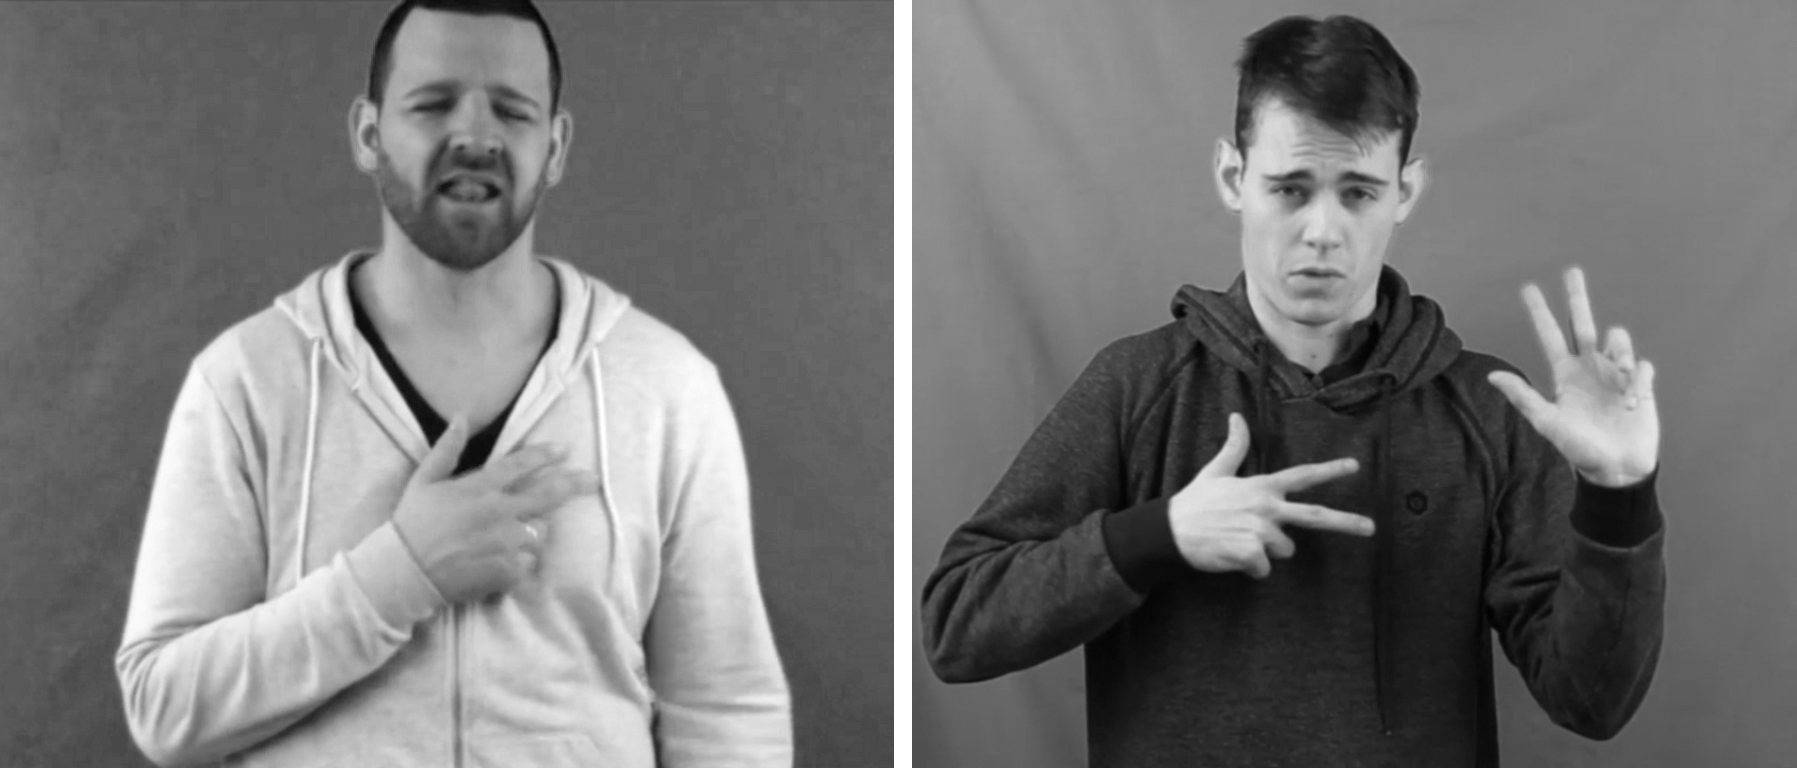
\includegraphics[width=1.0\textwidth]{honestlysw.jpg}
	\caption{The non-manual marker used with the speech-act adverb \textsc{honestly} consists of lifting the inner parts of the brows. On the left: \textsc{honestly} in a more positive sentence (\textit{Honestly, I'm very happy}). On the right: \textsc{honestly} used in a more apologetic context (\textit{Honestly, I don't know the book}).}
	\label{fig:honestly}
\end{figure}

To conclude this section, speech-act-indicating expressions which are of the \textit{honestly}/\textit{frankly} type can be expressed non-manually only or by the combination of a manual adverb and the respective non-manual marking. While expressing this category only non-manually is possible in DGS, there are more evaluations present in \textit{honestly}/\textit{frankly} contexts. The crucial non-manuals identified for this category are (the inner parts of) the eyebrows. As with the next categories to be discussed, the intensity of the non-manuals decreases towards the end of the clause.

\is{speech-act-indicating expressions|)}
\section{Mirative (\textit{surprisingly})}\is{mirative|(}


\subsection{General overview}

Mirative constructions encode the speaker's surprise about a proposition or that s/he did not expect the proposition to be true. \citet[85]{cinque1999adverbs} does not distinguish between evaluative adverbs like \textit{fortunately} and mirative adverbs expressing surprise such as \textit{surprisingly}. Other authors have tried to merge mirativity with evidentiality (e.g., \citealt{guentcheva1996tro}). It has been recognized, however, that mirativity is a grammatical category in many languages (e.g., \citealt{delancey2001mirative, aikhenval2009evidentiality}):

\begin{quote}
In many languages, expressions of mirativity have no grammatical connection to evidential systems. Markers with ``mirative'' meanings co-occur with evidentials, they occupy different positions in verb structure and differ in their interrelation with other categories [\dots ]. \citep[436]{aikhenvald2012essence}
\end{quote}

\noindent As already noted, I assume the mirative phrase to be located rather high up in the structure (see also \citealt[317]{testcari2013}; \citealt[57--59]{varley2014evidentiality}; \citealt{alcazar2016minor} and the discussion on page \pageref{mirmir}); to be more precise, I assume it to be sandwiched between speech-act indicators and evaluation.

\begin{figure}[bt]
\centering
	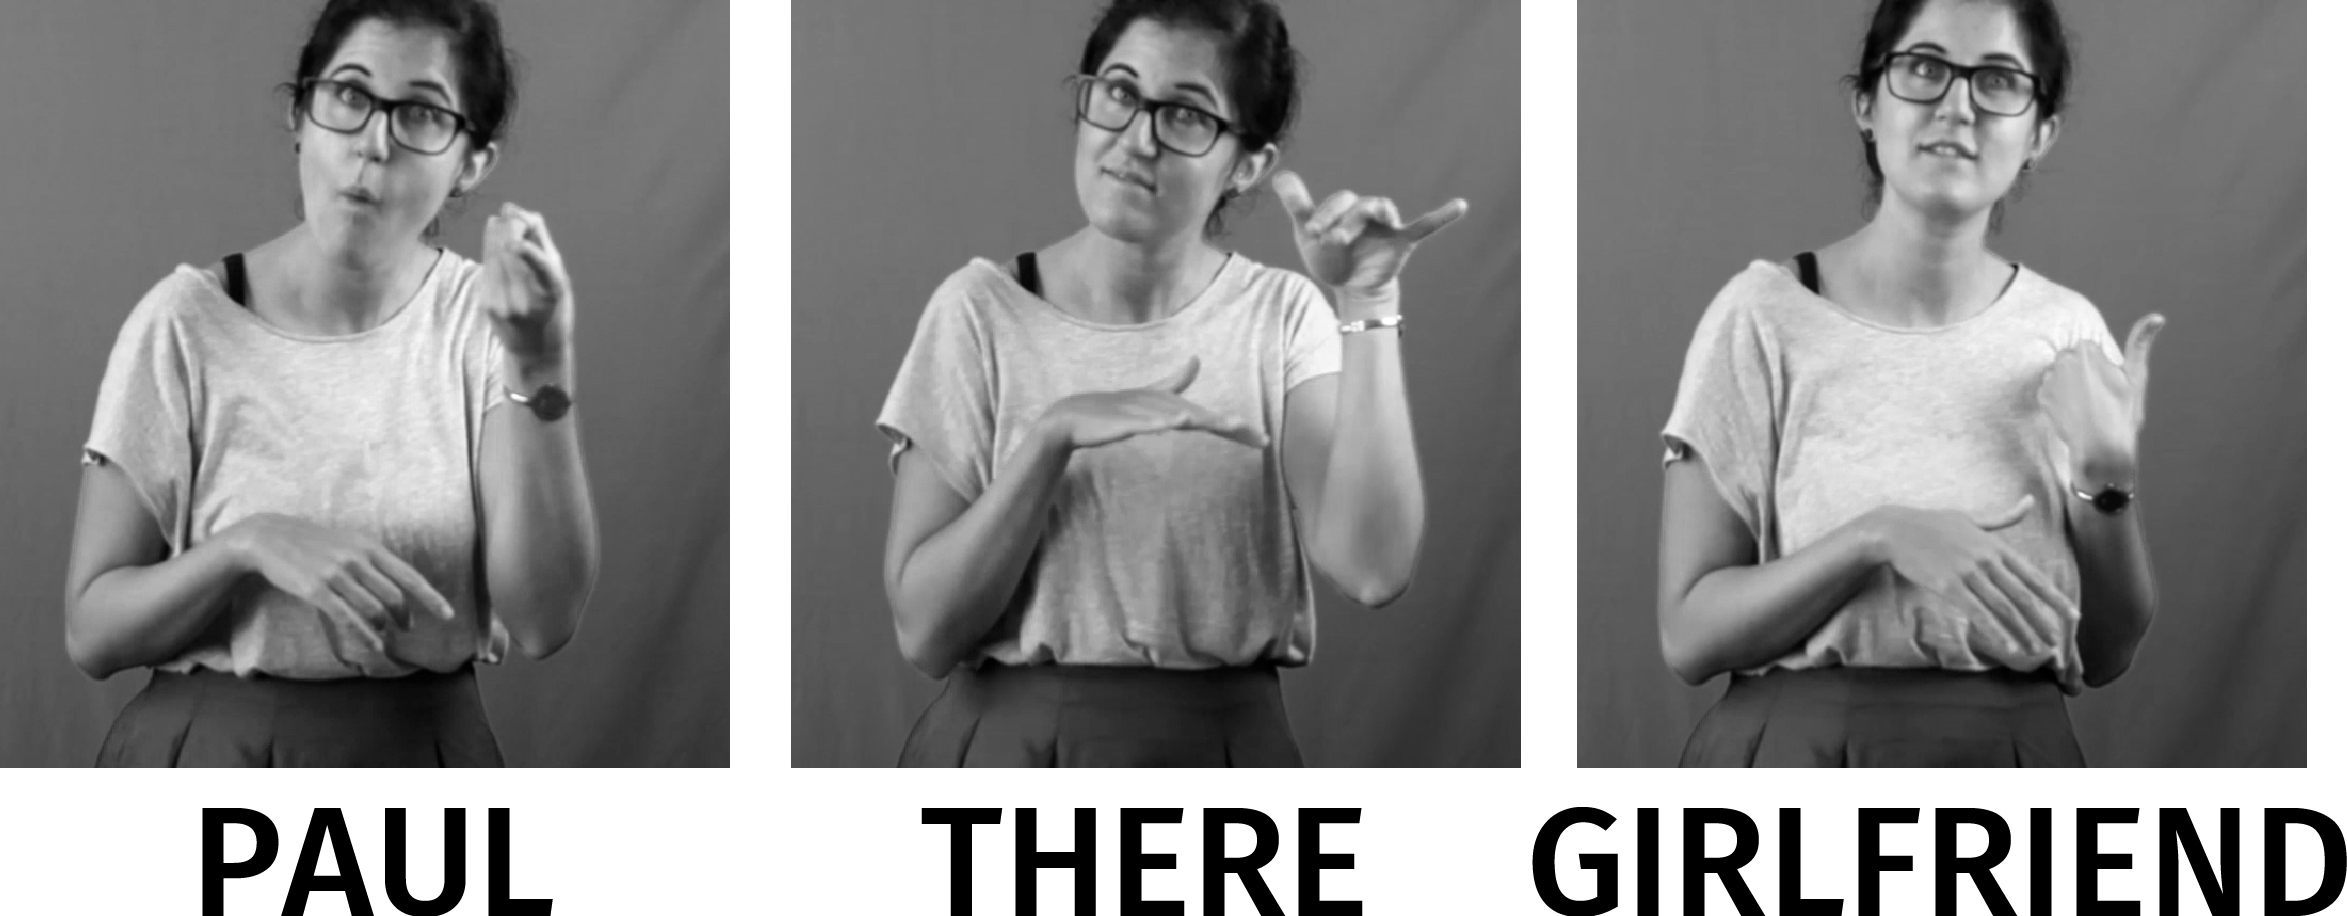
\includegraphics[width=1.0\textwidth]{mirative-nnmtwosw.jpg}
	\caption{The non-manuals used in mirative constructions: brow-raise, wide-open eyes, and leaning of the head (sometimes also the torso) forward.}
	\label{fig:mirative}
\end{figure}

\subsection{The situation in DGS}
Mirativity is, as expected, expressed non-manually in DGS, namely by a combination of brow-raise, wide-open eyes, and leaning of the head (sometimes also the torso) forward. This is illustrated for the sentence \textit{Surprisingly, Paul has a girlfriend} in Figure \ref{fig:mirative}. The non-manuals spread over the whole clause with the peak of intensity at the beginning and diminishing intensity towards the end of the clause. Note that the non-manuals are extremely similar to (if not exactly the same as) the non-manuals used in polar interrogatives. This similarity has been observed before. \citet[134]{herrmann2013modal}, for example, claims that raised brows therefore cannot be an indication of interrogativity. However, the spreading behavior in mirative constructions is exactly the opposite to that in polar questions: while the intensity in mirative constructions is highest at the beginning of the clause, the intensity of the non-manuals is highest towards the end of the clause in polar questions (cf. Section \ref{polarinterrogativesdgs}). 

As with other high categories in the Cinquean domain, it can be expressed non-manually only or by adding a clause-initial manual adverb, as shown in the examples in (\ref{ex:mirativitydgs}). In the case of mirativity, this can be either \textsc{surprisingly} or \textsc{really}. Again, the non-manuals are stronger when the manual adverb is absent. %This is shown


\begin{exe}
\ex\label{ex:mirativitydgs}\begin{xlist}
\ex \slgl[mirative]{paul computer new buy}
\glt `Surprisingly, Paul bought a new computer.'\label{ex:mirativitydgsa}
\ex \slgl[mirative]{surprisingly, paul computer new buy}
\glt `Surprisingly, Paul bought a new computer.'
\end{xlist}
\end{exe}

\noindent Note that the pause after the manual adverb, glossed by the comma in example (\ref{ex:mirativitydgsa}), seems to be obligatory. Nevertheless, mirativity is expressed either non-manually only or by the combination of this non-manual marking and a clause-initial manual adverb. Again, the intensity of the non-manuals is strongest at the beginning of the clause. Thus, the non-manuals in polar interrogatives and mirative constructions may seem to be the same superficially, but are distinct on closer examination: mirative non-manuals spread from left-to-right and polar interrogative non-manuals spread from right-to-left. This could be taken as evidence that the syntactic heads are left- and right-headed respectively. Alternatively, one could assume that both heads are left-headed and that XP movement is involved in the formation of polar interrogatives, but not in the case of mirative constructions.

\is{mirative|)}
\section{Evaluation (\textit{unfortunately})}\label{evalllll}\is{evaluation|(}

\subsection{General overview}

With evaluative adverbs or evaluative mood the speaker/signer expresses that s/he is evaluating a proposition as good or bad without changing the truth-value of the proposition. We are thus dealing with a speaker-oriented category as was already the case with speech-act indicating expressions and mirativity. 

\subsection{The situation in DGS}
Evaluation is expressed mainly non-manually in DGS. Depending on whether a proposition is evaluated as being good or bad, non-manuals differ. In both cases, however, a clause-initial evaluative adverb can be used. In this case, the non-manuals still have to be used. However, the non-manuals are stronger without a manual adverb. 

Figure \ref{fig:evalbad} shows an example of the evaluation of a proposition as being bad and Figure \ref{fig:evalgooda} shows an example of an evaluation of a proposition as being good.\footnote{ Note that the verb I have glossed \textsc{there} naturally precedes the object, resulting in an SVO structure. However, it is also allowed following the object. This seems to be a grammaticalization process. For many, but not all signers, the verb can have a copula use linking the subject with a predicate, e.g.,  \textsc{paul there hunger} `Paul is hungry'.\label{footnotecopula}} Both examples involve the use of a manual adverb. However, the non-manuals do not change without the use of a manual adverb -- with the exception that the non-manuals are stronger without the use of a manual adverb. A transcription of a sentence with and without a manual adverb is given in (\ref{ex:unfortgirlfried}).

\begin{exe}
\ex\label{ex:unfortgirlfried}\begin{xlist}
\ex \slgl[evaluation: bad]{unfortunately paul there girlfriend}
%
 %{\hspace{141pt}evaluation: bad}  \\
%{$\overline{\textrm{\textsc{unfortunately paul there girlfriend}}}$}     
\glt `Unfortunately, Paul has a girlfriend.' \label{ex:unfortgirlfrieda}
\ex \slgl[evaluation: bad]{paul there girlfriend}
%\ex
%\glll {${\hspace{117pt}\underline{\mathrm{\qquad evaluation: bad}}}$} \\
%\glll {\hspace{30pt}{}}  {\hspace{27pt}${\hspace{33pt}\underline{\textrm{\quad hn + ec}}}$} \\
 %{\hspace{55pt}evaluation: bad}  \\
%{$\overline{\textrm{\textsc{paul there girlfriend}}}$}     
\glt `Unfortunately, Paul has a girlfriend.' \label{ex:unfortgirlfriedb}


\end{xlist}
\end{exe}

\begin{figure}[b]
\centering
	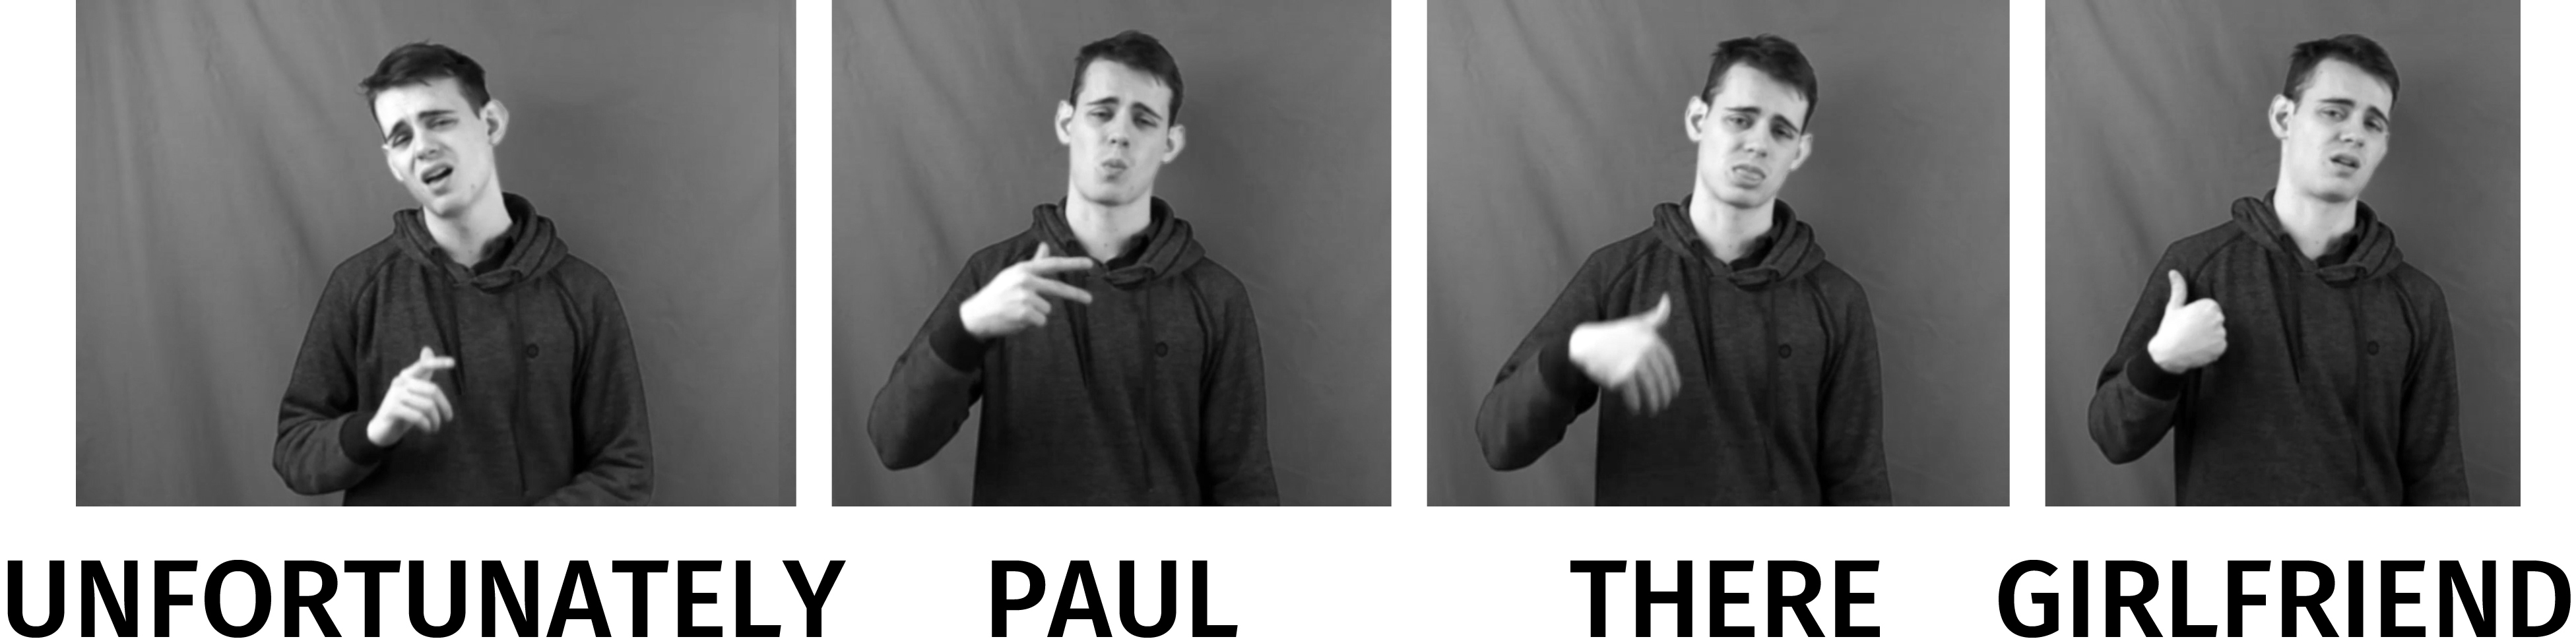
\includegraphics[width=1.0\textwidth]{evalbadsw.jpg}
	\caption{Evaluation as being bad. The sentence in this example is the translational equivalent of \textit{Unfortunately, Paul has a girlfriend}. The main markers are the eyebrows. Note that the movement of the head in this example cannot be observed in all instances of evaluation as bad. Thus, I do not take them to be part of the evaluative meaning.}
	\label{fig:evalbad}
\end{figure}

\begin{figure}[bt]
\centering
	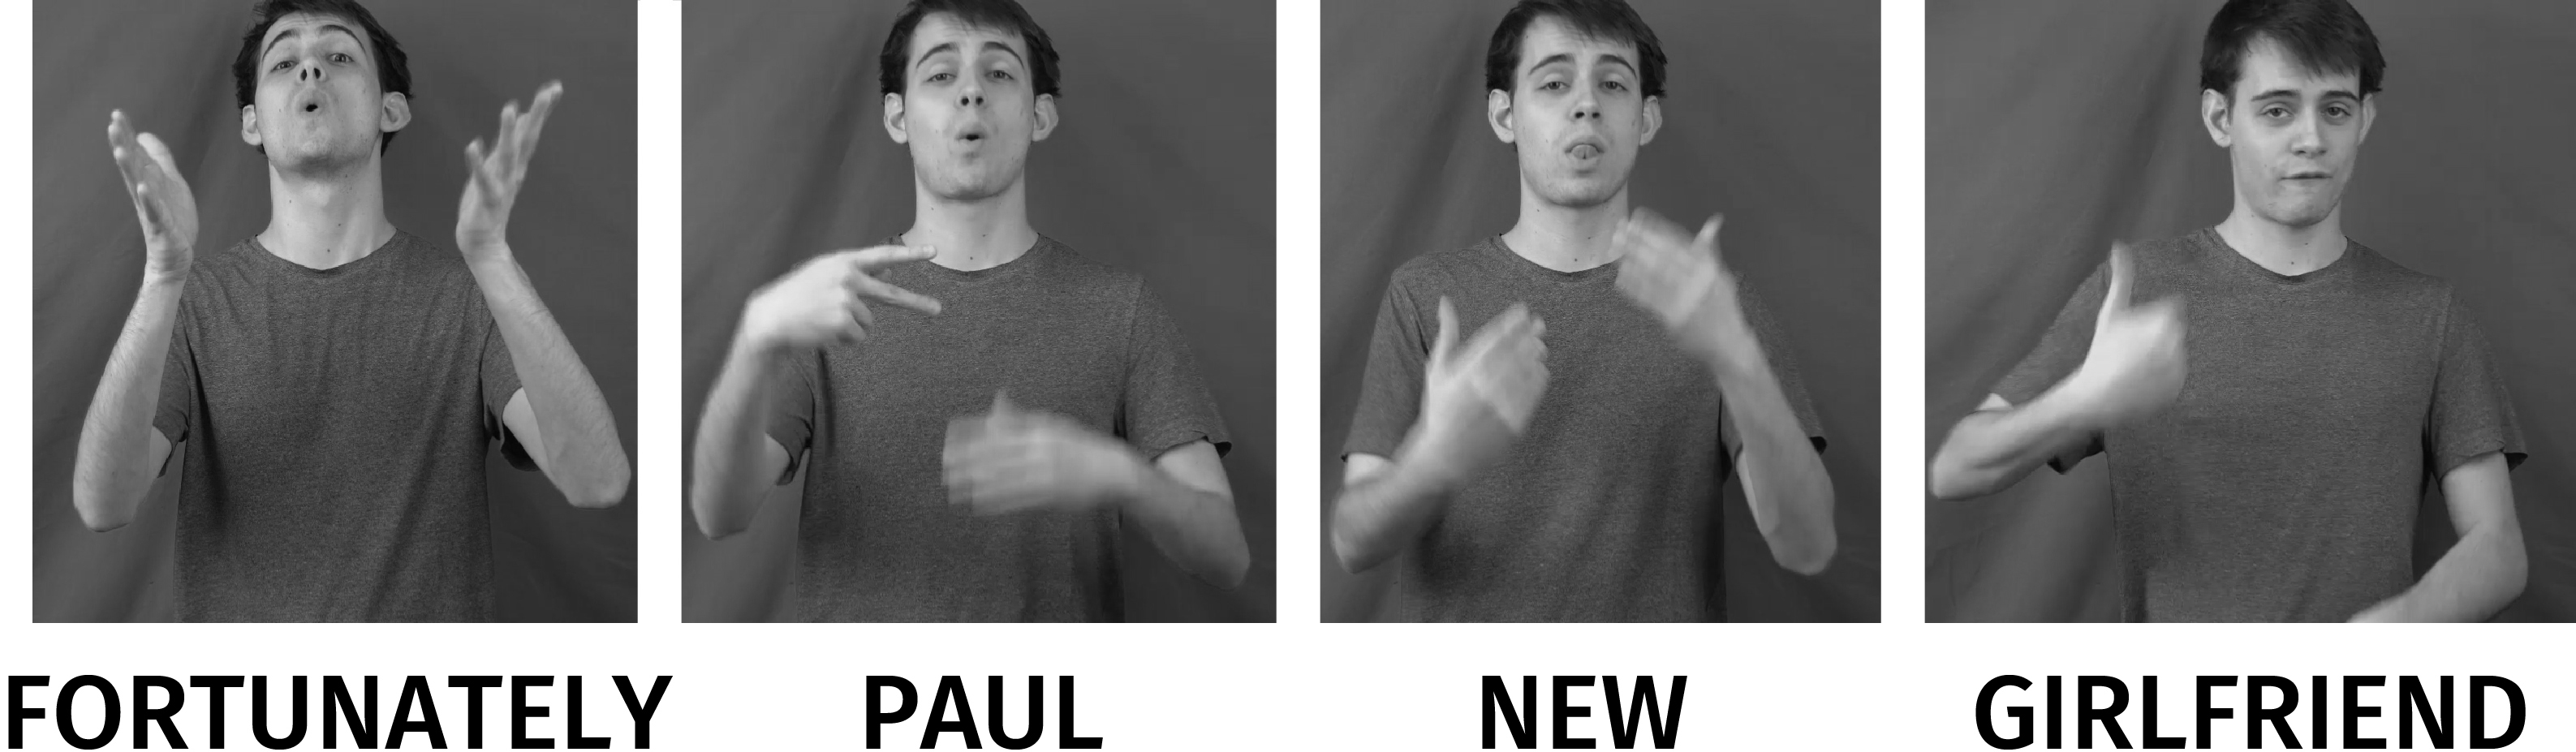
\includegraphics[width=1.0\textwidth]{evalgoodnewsw.jpg}
	\caption{Evaluation as being good. The sentence in this example is the translational equivalent of \textit{Fortunately, Paul has a new girlfriend}. The main markers are the eyebrows. Additionally, wide-open eyes are often observed in evaluation-as-being-good contexts.}
	\label{fig:evalgooda}
\end{figure}


\noindent The examples illustrate that both types of evaluation are marked with the eyebrows and the eyes. In the case of an evaluation as bad, this is expressed as a combination of raising the inner parts of the eyebrows and a squint and in the case of evaluation as good, a combination of raising the eyebrows and often wide-open eyes.  As with other high categories discussed in this chapter, the non-manuals are stronger when the manual adverb is absent and the intensity peak of the non-manuals is at the beginning of the clause. 


This category, thus again, employs a non-manual-only or a non-manual strategy combined with a clause-initial manual adverb. Again, the non-manuals are strongest at the beginning of the clause. The same observation will be made for evidentiality, the next category to be discussed.
\is{evaluation|)}

\section{Evidentiality (\textit{allegedly})}\label{evidentiality}\is{evidentiality|(}


\subsection{General overview}

While many languages have an elaborate system of evidential markers marking the source of the evidence of a piece of information, many others simply distinguish between direct and indirect evidence. In the latter kind of system, direct evidence is typically unmarked. Regardless of the system's structure, its realization can consist of affixes, particles, modal auxiliaries, or evidential adverbs. In German, for example, there is a distinction between two kinds of evidentialities: hearsay (also called `quotative' or `reportative') evidence and evidence by the subject. Both are marked with modal verbs. Hearsay evidence is encoded with the use of the modal verb \textit{sollen} `should', as in (\ref{germanreportativea}), evidence by the subject is realized with the modal verb \textit{wollen} `want' as in (\ref{germanreportativeb}).\footnote{ To be more precise, the modal verb \textit{sollen} is used to express a report by the subject when referring to the speaker. }

\begin{exe} 
\ex German \begin{xlist} 
\ex \gll {\textit{Laurita}} {\textit{soll}} {\textit{im}} {\textit{Lotto}} {\textit{gewonnen}} {\textit{haben}.}  \\
{Laurita} {should} {in-the} {lottery} {won} {have}\\
\trans `Laurita is said to have won the lottery.' \label{germanreportativea}
\ex \gll {\textit{Laurita}} {\textit{will}} {\textit{im}} {\textit{Lotto}} {\textit{gewonnen}} {\textit{haben}.}  \\
{Laurita} {wants} {in-the} {lottery} {won} {have}\\
\trans `Laurita, she claims, has won the lottery.' \label{germanreportativeb}
\end{xlist} 
\end{exe}

\noindent Other strategies include the use of evidential adverbs. This is, for example, the case with the English adverbs \textit{allegedly} or \textit{obviously}. 

\subsection{The situation in DGS}
Examples including adverbs like \textit{allegedly} find their translation to DGS either via the manual adverb \textsc{allegedly} or via non-manuals only -- although it has to be noted that most signers claimed to use the manual adverbs \textsc{allegedly} and \textsc{obviously} (see below) only rarely and mainly use the non-manual strategy. The non-manual markers relevant in this case are a squint and tensed eyes spreading over the whole clause. I glossed this set of non-manuals `allegedly' in the examples in (\ref{ex:allegedly}). When the manual adverb \textsc{allegedly} is present, the non-manuals still spread over the whole clause, but their intensity is reduced (in both cases the intensity peak is, again, at the beginning of the clause). Without the manual adverb, a sideward tilt can be observed accompanying the verb. I glossed this inclination `st' in the example in (\ref{ex:allegedlya}), see also Figure \ref{fig:allegedly} on the left. The example in (\ref{ex:allegedlyb}) shows the same sentence with the manual adverb \textsc{allegedly}. In this case, the inclination of the head is missing (for a discussion of the head position, see Section \ref{perhapsmoodirrealis} on page \pageref{perhapsmoodirrealis}). In line with the principle of analogical designation (see page \pageref{analogicaldesignation}), the non-manuals used in epistemic modality and evidentiality are very similar (or, alternatively, the categories coincide).

\begin{exe}
\ex\begin{xlist}\label{ex:allegedly}
\ex\label{ex:allegedlyb} \slgl[allegedly]{allegedly, paul lottery win}
%{\hspace{130pt}allegedly}  \\
%{$\overline{\textrm{\textsc{allegedly, paul lottery win}}}$}     
\glt `Allegedly, Paul has won the lottery.'
\ex\label{ex:allegedlya} \slgl[allegedly]{paul lottery \slg[\textup{st}]{win}} 
%\glll {${\hspace{88pt}\underline{\textrm{\textcolor{white}{w}st}}}$} \\
 %{\hspace{61pt}allegedly}  \\
%{$\overline{\textrm{\textsc{paul lottery win}}}$}     \\
\glt `Allegedly, Paul has won the lottery.'
\end{xlist}
\end{exe}

\begin{figure}[bt]
\centering
	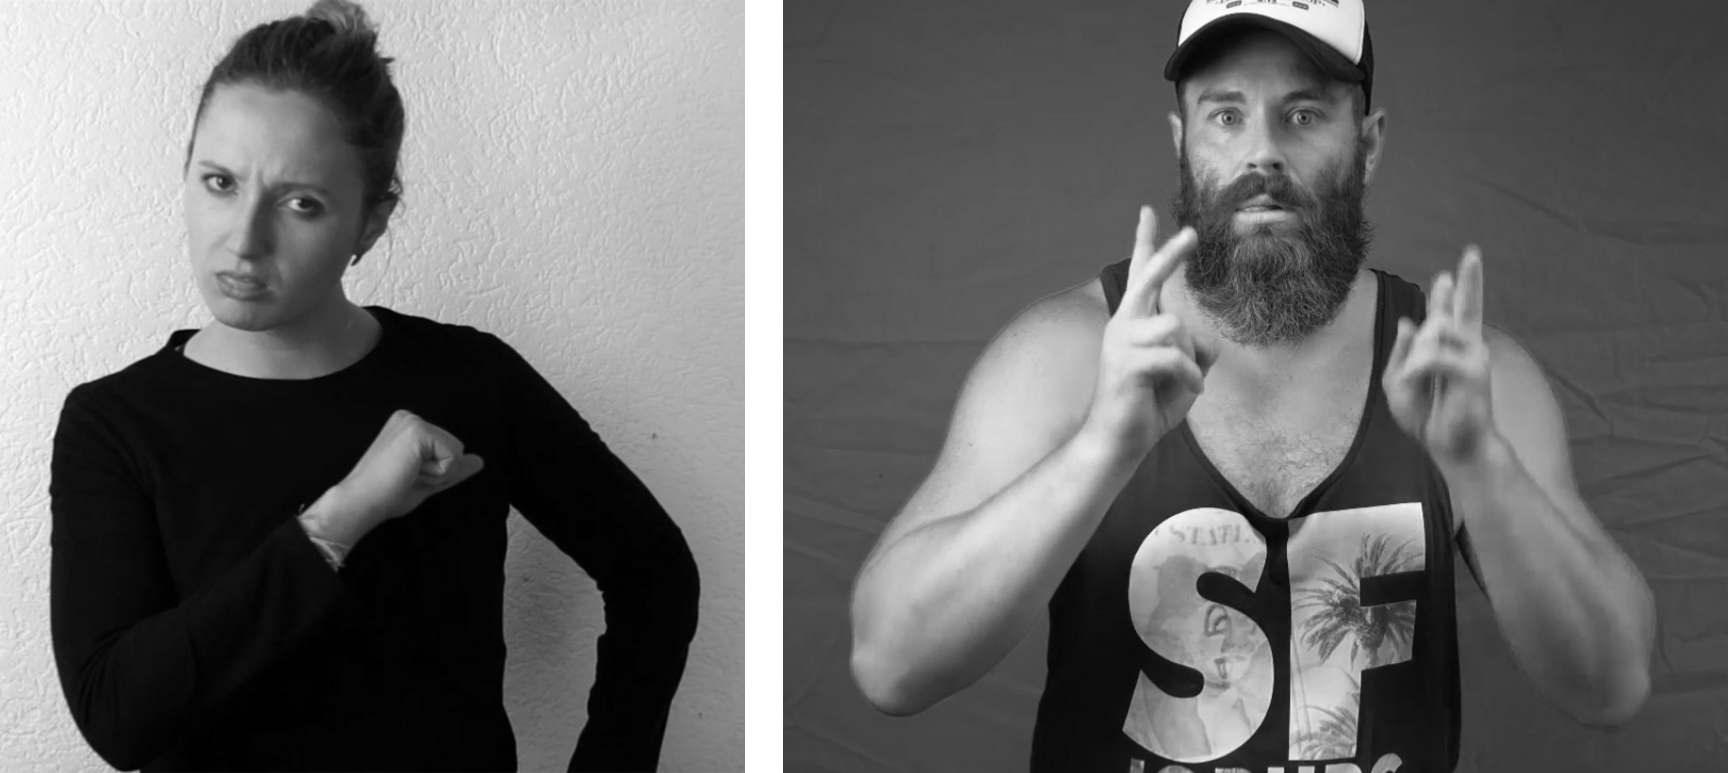
\includegraphics[width=1.0\textwidth]{allegedly-evidential3sw.jpg}
	\caption{1: Squinted brows and a slanted head are used for the encoding of evidentiality (\textit{allegedly}). 2: Wide-open eyes as a marker of obviousness.}
	\label{fig:allegedly}
\end{figure}

\noindent Examples including the adverb \textit{obviously} can be expressed in two ways: either by using the manual adverb \textsc{obviously} in combination with non-manual marking or by a non-manual-only strategy. The key non-manuals in both cases are wide-open eyes (not necessarily with a brow-raise), often accompanied by a forward lean of the head and/or body. Additionally, head nods accompany examples expressing obvious evidence (see also \citealt[133]{herrmann2013modal}). The non-manuals are shown in Figure \ref{fig:allegedly} on the right. 

\begin{exe}
\ex\label{ex:obiousness} \slg[top]{paul} \slgl[obvious]{now fast work}
%{\quad top} {\hspace{50pt}obvious}  \\
%{$\overline{\textrm{\textsc{paul}}}$} {$\overline{\textrm{\textsc{now fast work}}}$}     
\glt `Paul is obviously working fast now.'
\end{exe}

\noindent The mentioned non-manuals, wide-open eyes, head nods, and the forward head lean are glossed `obvious' in the example. While the non-manuals spread over the whole clause, their intensity diminishes towards the end of the sentence. Again, when a manual adverb is used, the non-manuals still obligatorily spread over the clause, however with less intensity.


I assume that wide-open eyes are generally an evidentiality marker (or a com\-mon-ground-managing device). This means that they mark a proposition as being shared by the interlocutors and can be paraphrased as `as is clear to us' or `as we both have direct evidence'.\label{obviousness} This observation is in line with previous findings on the marking of obvious evidence in DGS \citep[133]{herrmann2013modal}. In some cases, as will be discussed in section \ref{sectionepistemic}, the opposite marking, namely closed eyes, can mark the fact that a piece of information has not (yet) been shared by the interlocutors, a meaning that can be paraphrased as `as is clear to me' or `as only I have evidence for it'. Here the transition between evidentiality and epistemicity seems to be blurred.

To conclude this section, evidentiality is marked either non-manually only or by the combination of a manual adverb appearing clause-initially and the respective non-manual markers. Again, the non-manuals are located on the upper-face and again their intensity is strongest at the beginning of the clause.

Before turning to the discussion of the next lower category, namely epistemic modality, I will briefly introduce the notion of modality and make some remarks on the different modal flavors that will be distinguished in this chapter.

\section{A note on modality}\label{anoteonmodality}%\is{modality}
As the modality terminology in this book differs from the one used by Cinque, this section will briefly summarize the different modal flavors that will be relevant for the discussions to follow (for the term `modal flavor', see the side-note below). In the (generative) literature, usually three types of modality are distinguished: epistemic, deontic, and dynamic modality. Epistemic modality refers to ``the speaker's degree of confidence about the truth of a proposition'' \citep[86]{cinque1999adverbs}, given the information s/he has. Deontic modality is usually defined as the modality that ``is generally dependent on some kind of authority'' \citep[70]{palmer2001mood}. Finally, under the umbrella term `dynamic modality', \citet[196]{portner2009modality}, for example, counts ``modals of ability, disposition, and the like''. 

\begin{digression}{{Modal force, modal flavor, and modal anchor}}{}
\noindent The goal of this side-note is to provide the reader not familiar with the basic notions of modality with some background on the meaning of the terms `modal force', `modal flavor', and `modal anchor'. To do so, I will briefly (and informally) introduce modality from a possible-world semantics perspective (in the spirit of \citealt{kratzer1981, kratzer1991}).\is{modal force}\is{modal flavor}\is{modal anchor}

Modality can be expressed by various means in natural languages, for example, by sentence adverbs (e.g., \textit{possibly}), affixes (e.g., do\textit{able}), or modal auxilaries (e.g., \textit{can}). In the following discussion, I will concentrate on the latter. There are two main distinctions to be made when it comes to modality: modal forces and modal flavors. Modality is concerned with either necessary or possible truths. The dimension of necessity versus possibility is called ``modal force'' (there are, thus, only two modal forces). Approaching modality from a possible-world perspective, modal force is the kind of quantification over possible worlds which can be universal or existential quantification. Universal quantification equates with necessity (e.g., \textit{must}) and existential quantification with possibility (e.g., \textit{can}). The second distinction relates to modal flavors. A modal flavor refers to the interpretation of the modality (e.g., epistemic, deontic, dynamic). While the modal force can be derived from the lexical meaning of a modal (at least in English), the modal flavor needs a context.

To understand a sentence involving a modal verb one must know which worlds are the relevant worlds to quantify over since modals are context-sensitive expressions. This information can be derived from the context in which the sentence was uttered. This is called the `conversational background'. The conversational background provides the premise needed to interpret a modal. That modals are context-sensitive can easily be shown by way of example. The sentence \textit{Paula must work} can either mean that the speaker comes to the conclusion that it is necessary that Paula works based on the evidence which is available to him (we are then dealing with epistemic modality) or that it is necessary that Paula works because someone with more social power than her forces her to work (we are then dealing with deontic modality). Note that the syntax of the two meanings differ, but this cannot be seen from the surface form of the English examples.

A \is{conversational background}conversational background is a set of propositions. Which set of propositions are relevant is determined by two factors: the modal base and an ordering function. In order to understand, for example, a sentence with epistemic flavor, the set of relevant propositions are those known by the speaker or the interlocutors (provided by world knowledge or some evidence).  The set of worlds in which these propositions are true is called the `modal base' (i.e., the basis on which a modal will be interpreted). The second ingredient is the so-called `ordering source', a function that orders propositions. The ordering source takes the propositions of the modal base and ranks them according to some ideal. Let us again take the example of epistemic modality. An epistemic modal base is defined as the set of worlds in which the relevant propositions known by the speaker (or some interlocutors) are true. However, not all of these propositions have the same probability. Some may be more far-fetched than others given the normal course of events. The normal course of events is, in this case, the ideal which the ranking (or ordering) depends on. The ordering source now ranks propositions which are more likely, given the normal course of events, higher. Thus, a sentence like \textit{Paula must work} gets an epistemic interpretation by a modal base telling us that given all we know and all the evidence we have, it must be the case that the individual named Paula works given that the world we are in is a `normal' world in which everything works the way it usually does.

The last term I want to briefly discuss is `modal anchor'. In order to interpret a sentence containing a modal, it is necessary to select a modal base. But how does one select a modal base? If I utter the sentence \textit{Paula must work}, the modal base could be the relevant propositions which are true, for example, given possible world(s) (e.g., the possible worlds in which everything I know is true), given a situation, or given an event. This is the modal anchor, i.e., the domain (a possible world, a situation, or event) from which the modal base is generated \citep{mckenzie2018latent}.   
\end{digression}


\noindent Another notion that is often used is `root modality'. This term is also often used in a very broad sense. \citet[44]{platzack1979semantic}, for example, defines root modality as the expression of ``necessity [\dots ], obligation, permission, volition, or ability on behalf of an agent, which usually, but not necessarily, is expressed by the [\dots ] subject of the sentence.''

Clearly, the definitions given so far are rather vague and most of the terms cover a fairly broad range of meanings. This is especially true for dynamic modality including volition and ability -- two semantically rather distinct concepts. Additionally, it is not yet clear why different modalities should be distinguished at all. 


At least syntactically, the literature agrees that the three core modalities, epistemic, deontic, and dynamic, show different behaviors: epistemic modality scopes higher than deontic and deontic modality scopes higher than dynamic modality. From these differences in syntactic height, it is usually derived that different modalities are represented via different functional heads (e.g. \citealt{cinque1999adverbs, wurmbrand2001finitive, butler2003minimalist}). Such height differences can be shown, for example, by the interaction of tense and a modal verb (see already \citealt{groenendijk1975modality}). The German examples in (\ref{wurmbrand2001a}) and (\ref{wurmbrand2001b}) from \citet[184]{wurmbrand2001finitive} show that the modal verb \textit{müssen} `must' can have an epistemic and a deontic reading (\ref{wurmbrand2001a}). This is, however, not true when the modal verb is under the scope of an overt tensed auxiliary like \textit{haben} `have' (\ref{wurmbrand2001b}). 



\begin{exe} 
\ex German \citep[184]{wurmbrand2001finitive}
\begin{xlist} 
\ex \gll {\textcolor{white}{\cmark}\textit{Sue}} {\textit{muss}} {\textit{zuhause}} {\textit{arbeiten}.}\\
{\textcolor{white}{\cmark}Sue} {must} {at-home} {work}\\
\trans \cmark`It must be the case that Sue is working at home.' \hfill{\textit{epis.}}\\
\cmark `Sue is obliged to work at home.' \hfill{\textit{deontic}}\label{wurmbrand2001a}
\ex \gll {\textcolor{white}{\cmark}\textit{Sue}} {\textit{hat}} {\textit{zuhause}} {\textit{arbeiten}} {\textit{müssen.}}  \\
{\textcolor{white}{\cmark}Sue} {has} {at-home} {work} {must} \\
\trans \xmark `It must have been the case that Sue is working at home.' \hfill{\textit{epis.}} \\
\cmark `Sue had an obligation to work at home.' \hfill{\textit{deontic}}\label{wurmbrand2001b} 
\end{xlist} 
\end{exe} 

%\begin{exe} 
%\ex German \citep[184]{wurmbrand2001finitive}\begin{xlist} 
%\ex \gll   {\textcolor{white}{*$\cmark$}\textit{Sue}} {\textit{muss}} {\textit{zuhause}} {\textit{arbeiten.}}  \\
%{\textcolor{white}{*$\cmark$}{Sue} {must} {at-home} {work}  \\
%\trans \textcolor{white}{*}\cmark `It must be the case that Sue is working at home.' \hfill{\textit{epistemic}}\\
%\textcolor{white}{*}$\cmark$`Sue is obliged to work at home.' \hfill{\textit{deontic}}\label{wurmbrand2001a}
%\ex \gll  {\textcolor{white}{*$\cmark$}\textit{Sue}} {\textit{hat}} {\textit{zuhause}} {\textit{arbeiten}} {\textit{m\"ussen.}}  \\
%{\textcolor{white}{*$\cmark$}Sue} {has} {at-home} {work} {must} \\
%\trans \textcolor{white}{$\cmark$}*`It must have been the case that Sue is working at home.' \hfill{\textit{epistemic}} \\
%\textcolor{white}{*}$\cmark$`Sue had an obligation to work at home.' \hfill{\textit{deontic}}\label{wurmbrand2001b} 
%
%\end{xlist} 
%\end{exe} 

\noindent The examples suggest that when there is no overt tensed auxiliary, the syntactic position in which the modal is interpreted can switch as in (\ref{wurmbrand2001a}). This means that the modal can be interpreted as a higher epistemic or a lower deontic modal. However, when the syntactic surface forces us to interpret the modal as scoping below tense, as in (\ref{wurmbrand2001b}), only the deontic reading survives. This can be easily explained if we assume that the syntactic position of the epistemic modal is located above the tense projection (and the deontic modal is below tense). 

A similar argument can be made for the scopal interaction of modals and negation. In German, for example, \textit{müssen} takes scope above negation in an epistemic interpretation, while the same modal scopes below negation in a deontic reading as illustrated in (\ref{scopalinteractionnegmodal}).

\begin{exe} 
\ex German \\ \gll {\textit{Katie}} {\textit{muss}} {\textit{nicht}} {\textit{zuhause}} {\textit{sein}.} \\
{Katie} {must} {not} {at-home} {be} \\
\trans `It must be the case that Katie is \textit{not} at home.' \hfill{\textit{epistemic}}\label{scopalinteractionnegmodal} \\
`It is \textit{not} the case that Katie is obliged to be at home.' \hfill{\textit{deontic}}
\end{exe} 

\noindent The example shows that negation is interpreted above deontic, but below epistemic modality. We thus find the order $\minushookdown > \medsquare$ in deontic and the order $ \medsquare > \minushookdown$ in epistemic readings (e.g., \citealt{butler2003minimalist, iatridou2010scopal}). This, again, suggests that epistemic modality scopes higher, and is thus in a higher syntactic position than deontic modality.

Before turning to the discussion of the modal flavors used in this study, it is worth noting that there is yet another modal flavor often discussed in the literature, namely alethic modality. While epistemic modality is about the speaker's knowledge and beliefs, alethic modality is concerned with the necessary or contingent truth of a proposition (see also \citealt[28]{nuyts2000epistemic}). \citet{cinque1999adverbs} offers a detailed discussion on alethic modality and locates it below tense -- in stark contrast to epistemic modality. I will follow the more traditional account in that I assume that epistemic and alethic modality do not differ linguistically as it seems impossible to me for a speaker to differentiate between her/his knowledge and necessary or contingent truths in general. In Section \ref{alethicmodal} I will discuss alethic modality in some detail. In this section, I will show that the expression of alethic modality does not differ from epistemic modality in DGS.

The classification used in this study will differ slightly from what was proposed in the literature so far. Based on the definitions used in \citet{bross2017swabian}, I define the following modal flavors (already in their assumed order in syntax):

\begin{exe}
\ex\label{bsp:differentmodalitiesused} 
{\footnotesize $[$\textit{Epistemic}: What can or must hold in the view of what the speaker knows. \\
\textcolor{white}{n}$[$\textit{Bouletic/Volition}: What can or must hold in view of what the subject wants. \\
\textcolor{white}{nn}$[$\textit{Deontic}: What can or must hold in view of what the asymmetric power  \\
\textcolor{white}{nn\textit{Deontic} : }relations are like.\\
\textcolor{white}{nnn}$[$\textit{Root}: What can hold in view of the inherent properties of the modal anchor. \\
\textcolor{white}{nnnn}$]]]]$ }
\end{exe} 

\noindent Note that not all modalities are able to express both modal forces. So, while there is both epistemic necessity (e.g., English \textit{must}) and epistemic possibility (e.g., English \textit{could}), root modality, for example, is restricted to possibility (i.e., ability). For ease of understanding, (\ref{examplesmodalities}) gives some examples for each modality.

\begin{exe} 
\ex \label{examplesmodalities}\begin{xlist} 
\ex  The light is on, Ronnie \textit{must} be at home.  \hfill\textit{epistemic} \label{examplesmodalitiesa}
\ex  Elias \textit{wants} to go to the beach.  \hfill\textit{bouletic/volition} \label{examplesmodalitiesb}
\ex  Carsten's parents are strict, he \textit{must} be home early.  \hfill\textit{deontic} \label{examplesmodalitiesc}
\ex  Ricarda \textit{can} play the guitar very well.  \hfill\textit{root} \label{examplesmodalitiese}
\end{xlist} 
\end{exe} 

\noindent It is likely that there are more modal flavors to be distinguished (e.g., circumstantial modality that is about causalities affecting the relevant participant), but I will restrict myself to the flavors listed in (\ref{bsp:differentmodalitiesused}) and exemplified in (\ref{examplesmodalities}). In the next section, I discuss the expression of the highest modal flavor, i.e., epistemic modality.  

\section{Epistemic modality (\textit{probably})}\label{sectionepistemic}\is{epistemic modality|(}
\subsection{General overview}
In English, as in many other languages, epistemic modality can be expressed via modal verbs, like \textit{must}, or with epistemic adverbs, like \textit{probably}. \citet[86]{cinque1999adverbs} assumes that epistemic modals and epistemic adverbs are both located in the same projection. While epistemic modals occupy the head of this projection, epistemic adverbs occupy the specifier of this projection. 

For sign languages, it has often been observed that modal verbs used for deontic modality cannot be used in epistemic contexts, and when this is allowed they receive a special non-manual marking that is not present with deontic readings: ``In sign languages[\dots ] it seems to be the case that epistemic readings of modal verbs are rare, or at least quite marked, and that signers tend to interpret modal verbs as deontic markers only'' \citep[231]{signgram2017}.\footnote{ Note that the term `deontic' in the quote is used in the broad sense discussed in the previous subsection.} Additionally, epistemic modality is often expressed via non-manuals only as described mainly for \is{American Sign Language}American Sign Language (e.g., \citealt{wilcox1995gestural, wilcox1996deontic, shaffer2000syntactic, wilcox2006modality}). Similar observations have been made for DGS \citep{herrmann2013modal, happ2014vork, bross2017scope}.

\subsection{The situation in DGS}
The observations described above are fully in line with my own observations: epistemic modality is expressed non-manually only in DGS or by a combination of non-manual marking and an adverb, as shown in the examples in (\ref{ex:epistemichapp}) from \citet[364]{happ2014vork}.


\begin{exe}
\ex\label{ex:epistemichapp}\begin{xlist}
\ex \slgl[epistemic:poss]{(possibly) swen work go}
\glt `Swen could be off to work.'\label{epistemichappa}
\ex \slgl[epistemic:certain]{(certainly) swen work go}
\glt `Swen must be off to work.'\label{epistemichappb}
\end{xlist}
\end{exe}

\noindent As the examples illustrate, the use of the adverbs glossed \textsc{possibly} and \textsc{surely} is optional. The non-manuals used in (\ref{epistemichappa}) are described as consisting of a squint, slightly pulled down corners of the mouth, a head nod, and a slightly tilted torso by \citet[364]{happ2014vork}. The non-manuals in (\ref{epistemichappb}) are described as consisting of slightly squinted eyebrows, a head nod, and a slightly tilted torso.\footnote{ Furrowed brows and head nods were described in epistemic contexts for many sign languages, including \is{American Sign Language}American Sign Language \citep{wilcox2006modality} and \is{Austrian Sign Language}Austrian Sign Language \citep{lackner2017functions}.} Except for the pulled-down corners of the mouth, these descriptions are fully in line with my own observations. The head nod is mainly found accompanying the verb. Additionally, closed eyes can often be observed while nodding. I will gloss this `hn, ec' in the following.

Examples of signed sentences with and without the use of a manual adverb are given in Figure \ref{probablynmmmanual}. The crucial difference between the two examples is that the non-manuals are much stronger when the manual adverb is not used. In both cases, the peak of the non-manuals is clause-initial, i.e., the non-manuals accompany the whole clause but their intensity diminishes towards the end of the clause. The main non-manual marker of epistemicity are squinted eyebrows, often a raising of the inner parts, and a slanted head. The main marker, however, seems to be the squinting of the eyebrows (see also Figure \ref{epistemicobvious}).


\begin{figure}[bt]
\centering
	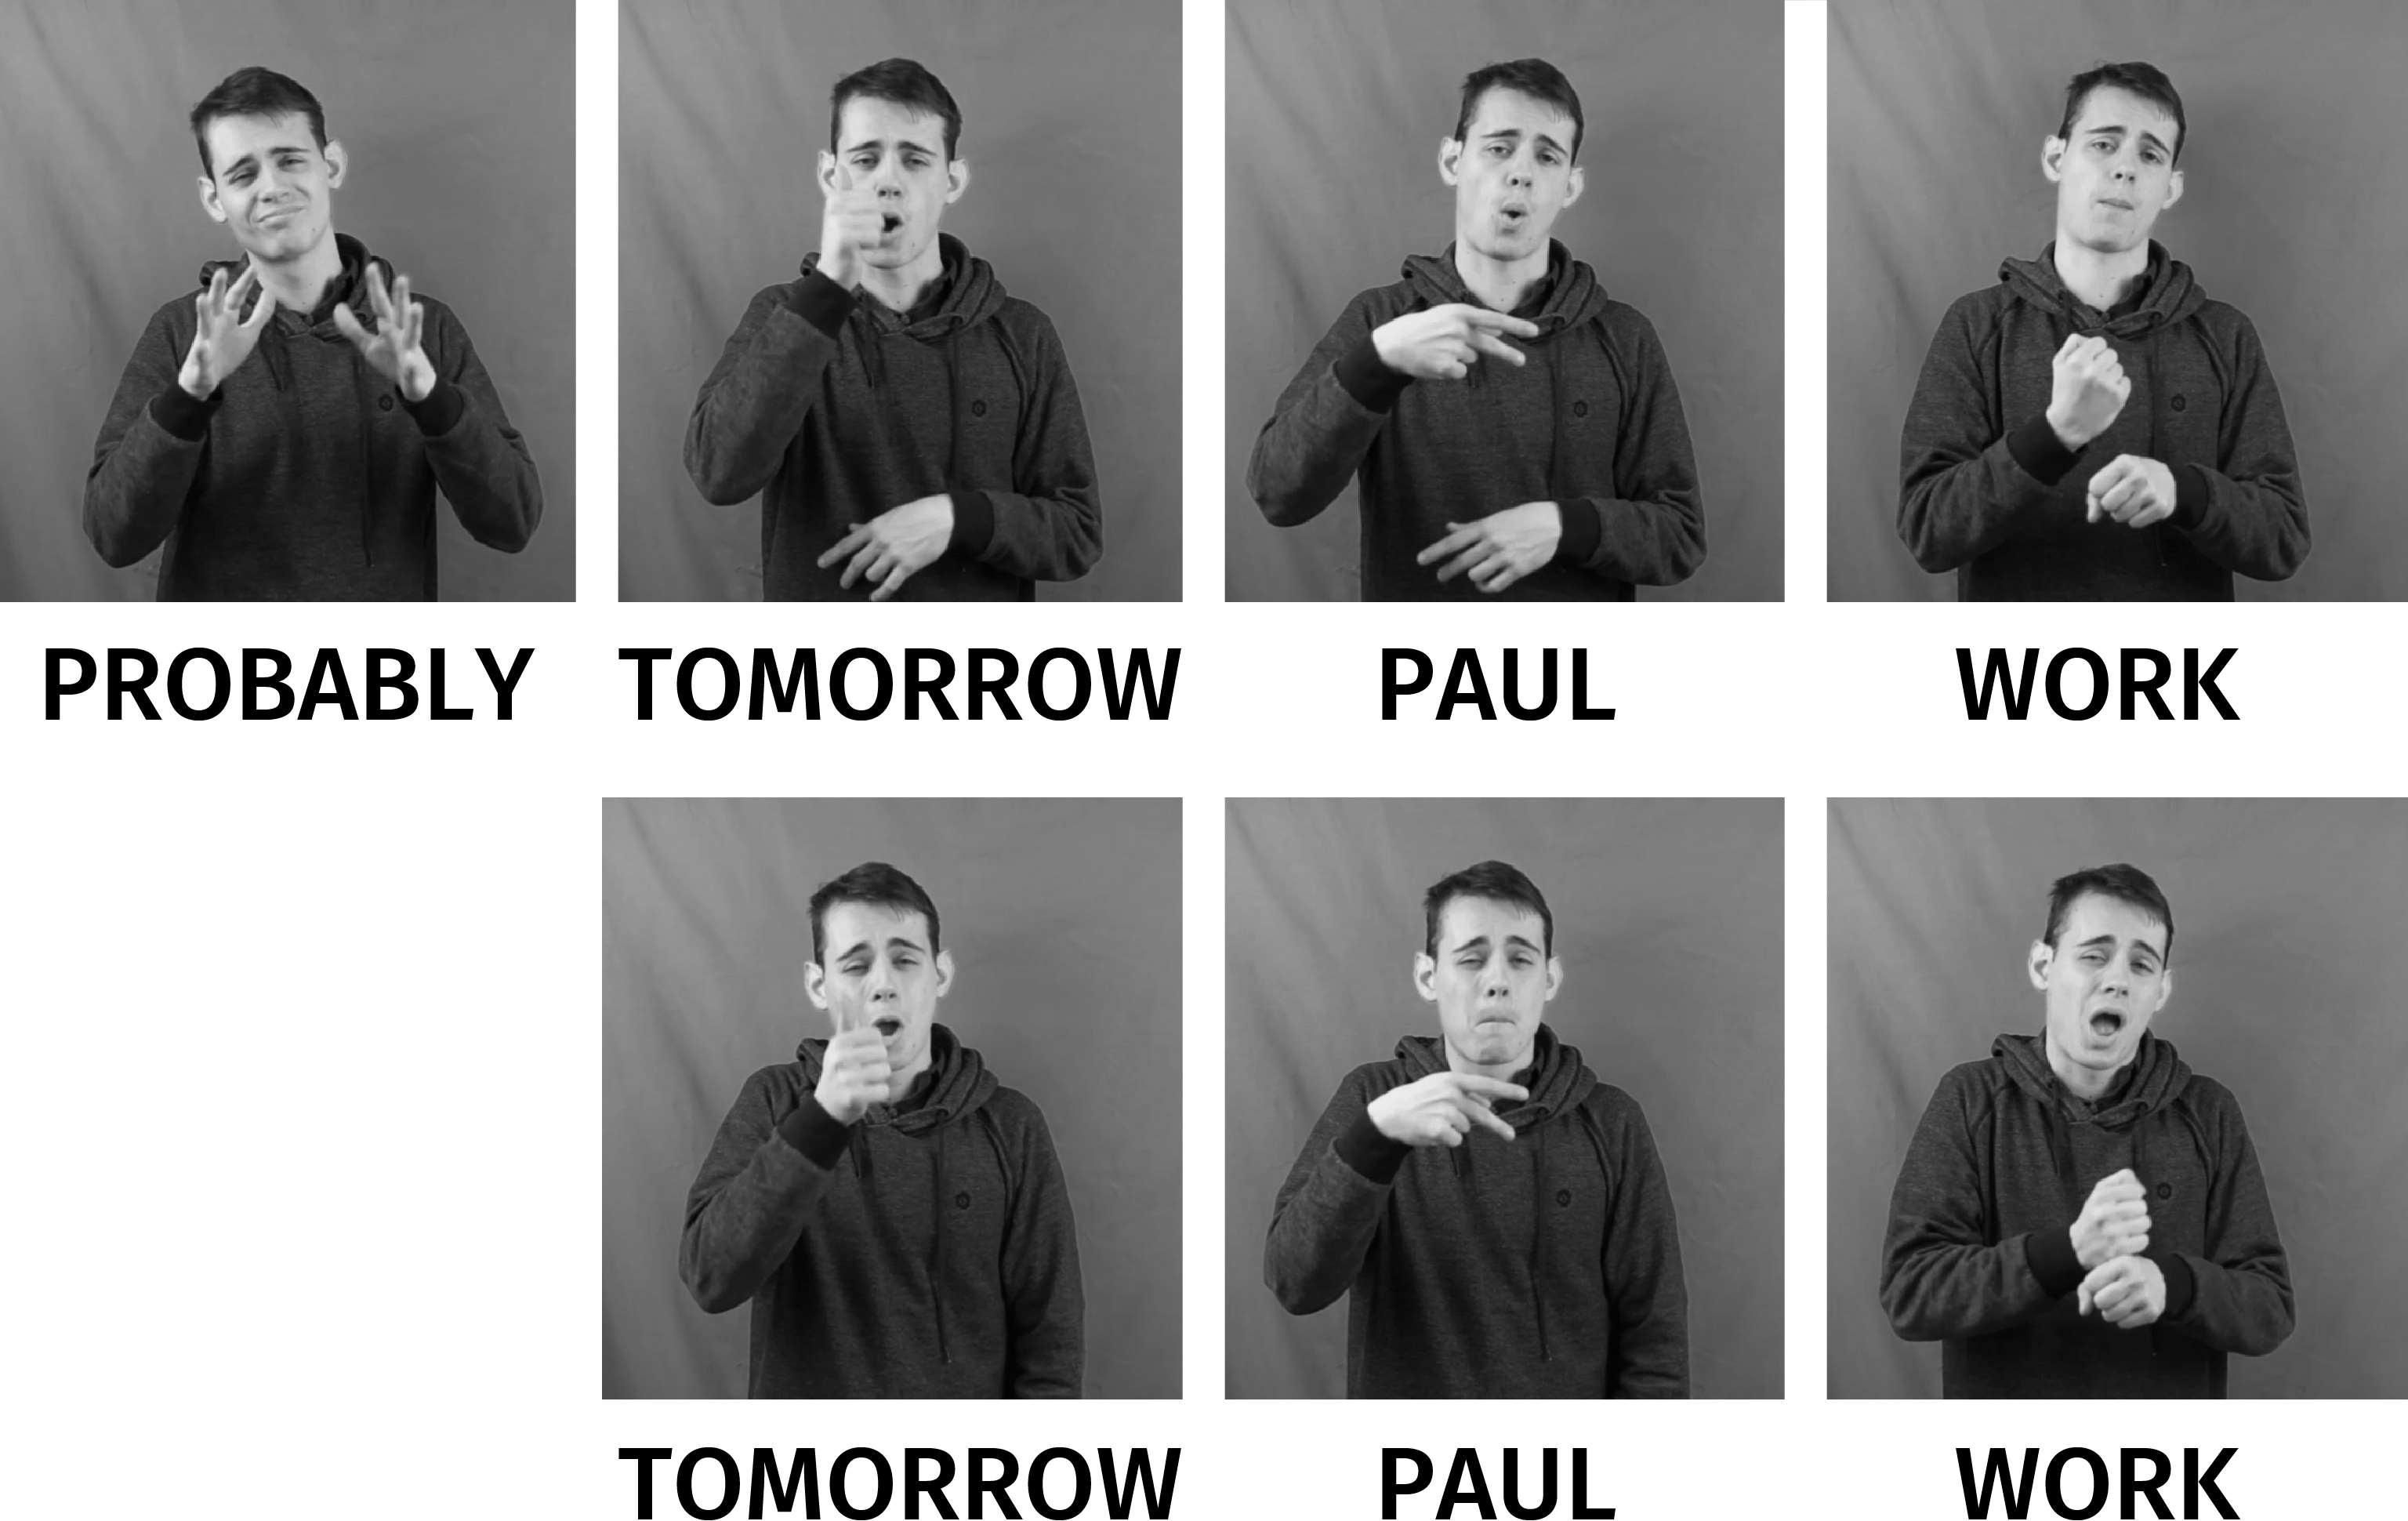
\includegraphics[width=1.0\textwidth]{probablysw.jpg}
	\caption{The translational equivalent of \textit{Paul probably works tomorrow}. The top sentence is an example of the use of a combination of the manual adverb \textsc{probably} and an epistemic non-manual marking. The bottom sentence is an example of the use of a non-manual-only strategy.}
	\label{probablynmmmanual}
\end{figure}

Modal verbs such as \textsc{must} or \textsc{can} cannot be used in epistemic contexts in DGS \citep[112]{herrmann2013modal} and, conversely, epistemic encoding in a structurally lower modal context is not possible. This is shown in the examples in (\ref{bsp:notconv}) (partially adapted from \citealt{bross2017scope}). 

\begin{exe}
\ex\label{bsp:notconv}\begin{xlist}
\ex \slg{index_{\textup{3a}} light existential} \slgl[epistemic]{paul \slg[\textup{hn, ec}]{at-home}} 
%\ex 
%\glll {}  {${\hspace{38pt}\underline{\textrm{\quad hn $+$ ec}}}$} \\
%{} {\hspace{41pt}epistemic}  \\
%{\textsc{index}\textsubscript{3a} \textsc{light there}} {$\overline{\text{\textsc{peter at-home}}}$}   \\
\glt `The light is on, Peter must be at home.'\label{bsp:notconva}
\ex \slg{index_{\textup{3a}} light existential} *\slgl[epistemic]{paul \slg[\textup{hn, ec}]{at-home must}} 
%
%\ex  
%\glll {}  {${\hspace{76pt}\underline{\textrm{\quad hn $+$ ec}}}$} \\
%{} {\hspace{80pt}epistemic}  \\
%{\textsc{index}\textsubscript{3a} \textsc{light there}} {*$\overline{\text{\textsc{peter at-home must}}}$}   \\
\glt `The light is on, Peter must be at home.'\label{bsp:notconvb}
\ex \slg{paul parents strict} *\slgl[epistemic]{paul \slg[\textup{hn, ec}]{at-home}} 
%
%
%\ex
%\glll {} {} {${\hspace{35pt}\underline{\textrm{\quad hn $+$ ec}}}$} \\
 %{} {} {\hspace{38pt}epistemic}  \\
%{\textsc{paul parents}} {\textsc{strict}} {*$\overline{\text{\textsc{paul at-home}}}$}    \\
\glt `Paul's parents are strict. Paul has to stay at home.'\label{bsp:notconvc}
\end{xlist}
\end{exe}

\noindent The examples illustrate that epistemic modality must be expressed non-manually (\ref{bsp:notconva}). It is not possible to use a manual modal like \textsc{must} in an epistemic context (\ref{bsp:notconvb}). Similarly, it is not possible to use the non-manual marking in a syntactically lower modality, as exemplified for deontic modality in the example in (\ref{bsp:notconvc}).

\begin{figure}[bt]
\centering
	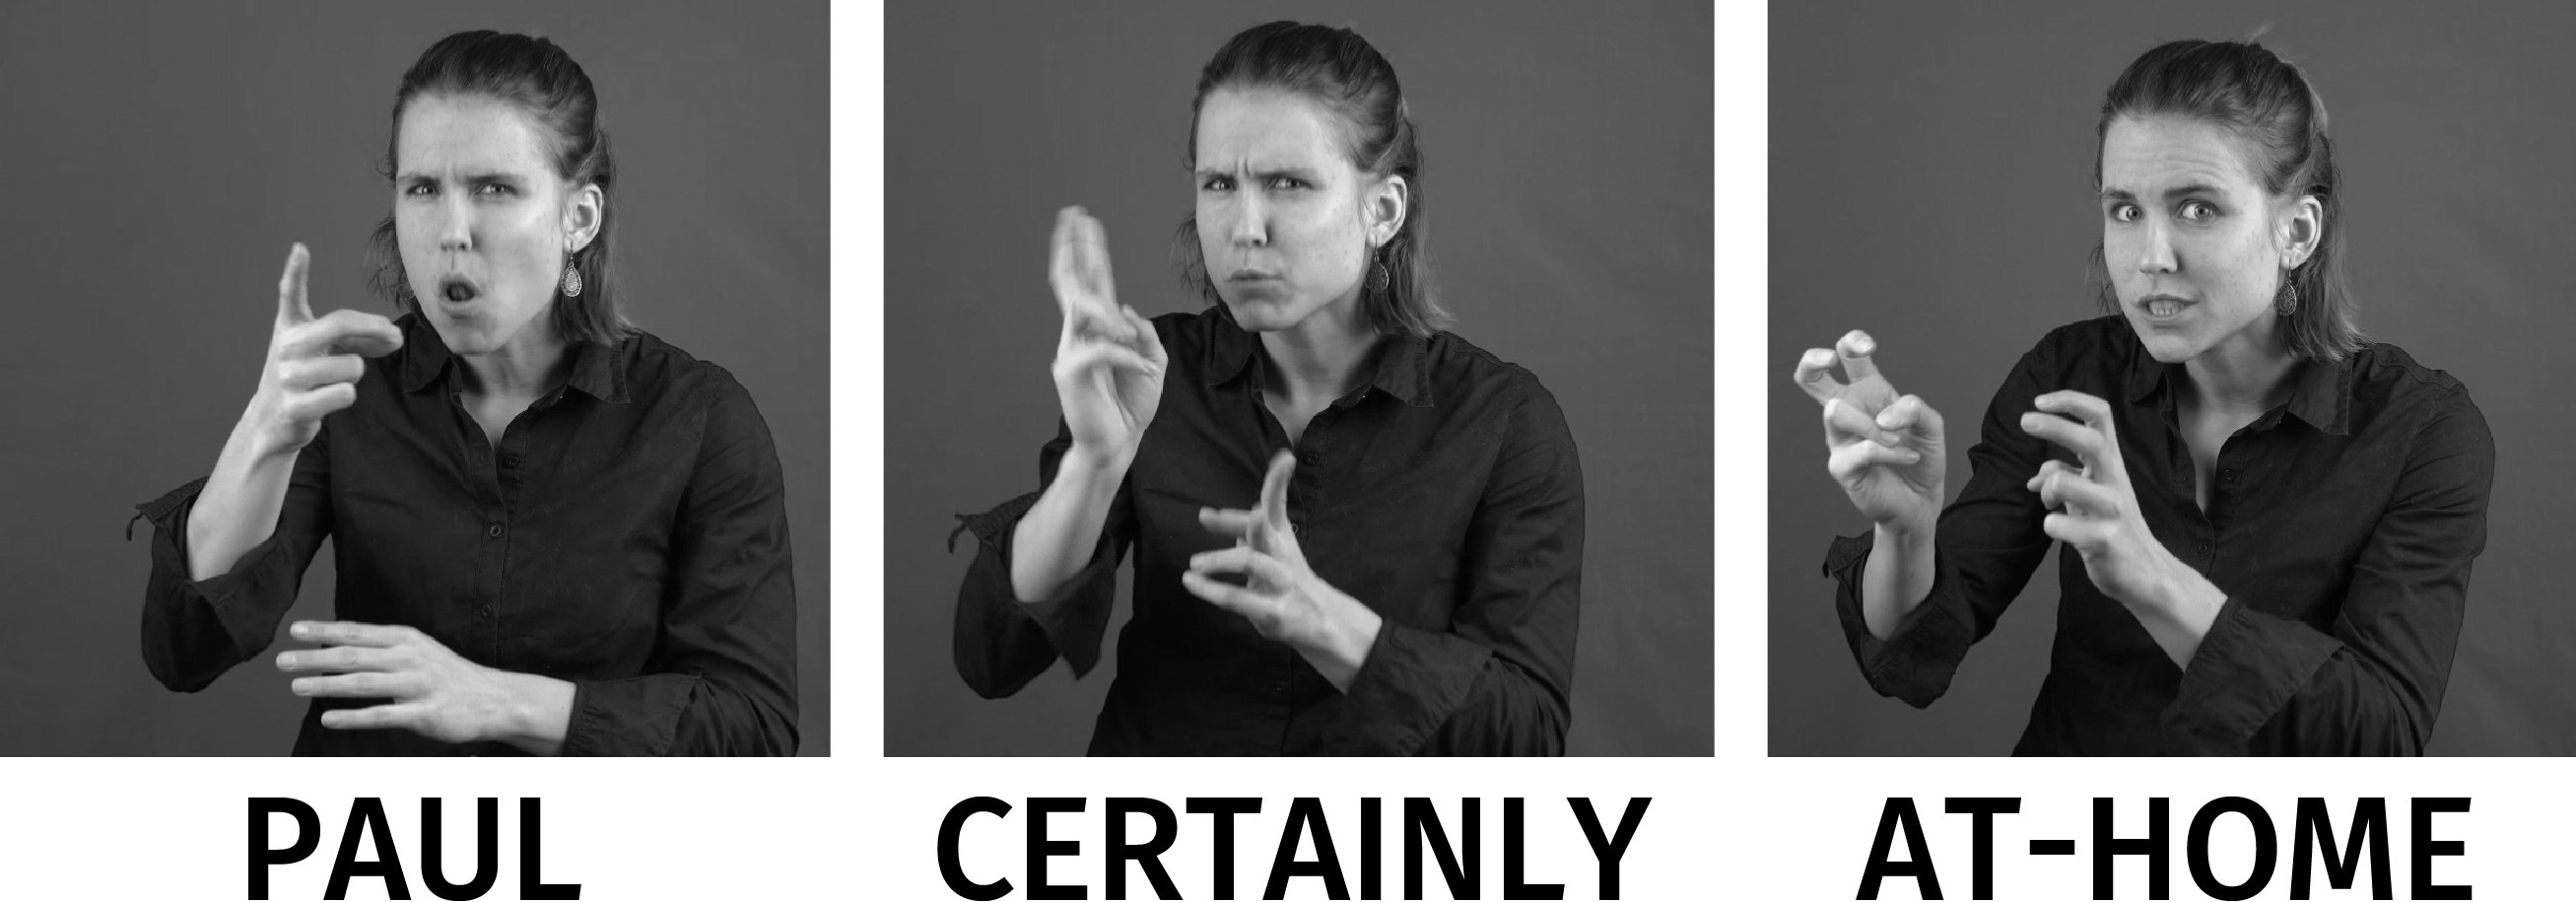
\includegraphics[width=1.0\textwidth]{epistemicobvioussw.jpg}
	\caption{The combination of evidentiality and epistemicity leads to a combination of non-manual markings. In this case, the interlocutors shared the knowledge that the light is on (\textit{See, the light is on. Paul must obviously be at home.})}
	\label{epistemicobvious}
\end{figure}

A last note relates to the similarity of evidentiality and epistemicity, two categories which are sometimes not easy to distinguish. Both categories can be expressed non-manually in one signed sentence. Wide-open eyes were already discussed as a common-ground/evidentiality marker on page \pageref{obviousness}. When combined with epistemicity, the wide-open eyes appear on the main predicate while the rest of the clause is marked with squinted eyebrows, as shown in Figure \ref{epistemicobvious}. The figure shows the epistemic sentence \textit{Paul must surely be at home}. In this case, however, the interlocutors shared the information that the light is on (the context was: \textit{See! The light is on! Paul must surely be at home.}). The certainty in this case is additionally expressed by holding the head straight instead of slanting it as in Figure \ref{probablynmmmanual}. For the head position, see also the discussion in Section \ref{perhapsmoodirrealis} on page \pageref{perhapsmoodirrealis}.

To sum up, all the categories in Cinque's hierarchy that have been discussed so far find their expression either non-manually (with the non-manuals spreading over the whole clause) or by a combination of a non-manual marker and a manual adverb that appears clause-initially. In all cases, the intensity of the non-manuals was observed to be strongest at the beginning of the clause.



\is{epistemic modality|)}

\section{Mood irrealis (\textit{perhaps})}\label{perhapsmoodirrealis}\is{irrealis|(}\is{mood irrealis|see{irrealis}}
Note that it was proposed to locate this category below tense in Cinque's system. I argue, however, that it should be located above tense instead.


\subsection{General overview}
In Italian, \citet[86--89]{cinque1999adverbs} observes that deictic temporal adverbs follow the epistemic adverb \textit{probabilmente} `probably' while the adverb \textit{forse} `perhaps' behaves differently as it does not precede but rather follows deictic temporal adverbs. However, he admits that the judgments he bases his facts on ``are rather delicate'' \citep[87]{cinque1999adverbs}, but nevertheless deduces the hierarchical order shown in (\ref{crazyorder}). For the category that is represented by adverbs like \textit{perhaps}, he uses the name `irrealis'.

\begin{exe} 
\ex probably (epistemic) $>$ deictic temporal adverbs $>$ perhaps (irrealis) \label{crazyorder}
\end{exe}  

\noindent Additionally, \citet[33]{cinque1999adverbs} claims that temporal adverbs in English also precede \textit{perhaps} and similar adverbs like \textit{almost certainly} (and thus, \textit{perhaps}, behave differently than epistemic adverbs that are not preceded by temporal adverbs). Cinque's data is shown in (\ref{cinuqeenglishdatairrealis}).

\begin{exe}
\ex\label{cinuqeenglishdatairrealis}\begin{xlist}
\ex \textcolor{white}{*}He was then almost certainly/perhaps at home.
\ex *He was almost certainly/perhaps then at home.
\end{xlist}
\end{exe}

\noindent This judgments, however, were disputed by native speakers of English \citep[32]{zyman2012two}. Additionally, corpus data show that both options are equally attested in English \citep[65--66]{nordstrom2010modality}. And there are more reasons to believe that epistemic adverbs and what Cinque calls `irrealis' either occupy the same syntactic position or are at least located above tense. First, it is not possible for epistemic adverbs and irrealis adverbs to occur in the same clause.\footnote{ But see \citet[32]{zyman2012two} who claims that, in English, this is at least marginally possible. As the conclusion he draws from this is merely that epistemic adverbs scope higher than irrealis adverbs, nothing hinges on that (as it tells us nothing about the question of whether irrealis adverbs are lower than tense). } Secondly, it is not only irrealis adverbs that are able to follow and precede temporal adverbs in English, but also epistemic adverbs, as noted in \citet[33]{cinque1999adverbs}. His examples are given in (\ref{cinuqeenglishdatairrealiscc}).

\begin{exe}
\ex\label{cinuqeenglishdatairrealiscc}\begin{xlist}
\ex Probably he once had a better opinion of us.
\ex Once he probably had a better opinion of us.
\end{xlist}
\end{exe}

\noindent The conclusion to draw from this data is that epistemic and irrealis adverbs have the very same distribution in English. The same holds true in German as both \textit{wahrscheinlich} `probably' and \textit{vielleicht} `perhaps' can either precede or follow deictic temporal adverbs, as illustrated in (\ref{spokengermantemporalprobalbyperhaps}).\footnote{ Asking a native speaker of Italian actually led to the very same results, namely, that both adverbs, \textit{forse} `perhaps' and \textit{probabilmente} `probably' can precede and follow deictic temporal adverbs, as shown in (\ref{italianforseperhaps}).

\begin{exe}
\ex Italian \label{italianforseperhaps}\begin{xlist} 
\ex \gll {\textit{Ieri}} {\textit{Paul}} {\textit{ha}} {\textit{prima}} {\textit{comprato}} {\textit{le}} {\textit{mele}} {\textit{e}} {(forse)} {\textit{poi}} {(forse)} {\textit{ha}} {\textit{fumato}} {\textit{una}} {\textit{sigaretta}}.\\
{yesterday} {Paul} {has} {first} {bought} {the} {apple} {and} {perhaps} {then} {perhaps} {has} {smoked} {a} {cigarette}\\ 
\trans `Yesterday Paul first bought the apples and then he perhaps smoked a cigarette.' \label{italianforseperhapsa}
\ex \gll {\textit{Ieri}} {\textit{Paul}} {\textit{ha}} {\textit{prima}} {\textit{comprato}} {\textit{le}} {\textit{mele}} {\textit{e}} {(probabilmente)} {\textit{poi}} {(probabilmente)} {\textit{ha}} {\textit{fumato}} {\textit{una}} {\textit{sigaretta}}.\\
{yesterday} {Paul} {has} {first} {bought} {the} {apple} {and} {probably} {then} {probably} {has} {smoked} {a} {cigarette}\\ 
\trans `Yesterday Paul first bought the apples and then he probably smoked a cigarette.' \label{italianforseperhapsb}

\end{xlist}
\end{exe}

}

\begin{exe}
\ex German\label{spokengermantemporalprobalbyperhaps}\begin{xlist} 
\ex \gll{\textcolor{white}{`}$[$\dots $]$} {\textit{dass}} {\textit{Gökce}} {(wahrscheinlich)} {\textit{davor}} {(wahrscheinlich)} {\textit{zuhause}} {\textit{war}}.\\
{\textcolor{white}{`}$[$\dots $]$} {that} {Gökce} {probably} {before} {probably} {at.home} {was}\\
\trans `$[$\dots $]$ that before that Gökce was probably at home.' \label{spokengermantemporalprobalbyperhapsa}
\ex \gll{\textcolor{white}{`}$[$\dots $]$} {\textit{dass}} {\textit{Gökce}} {(vielleicht)} {\textit{davor}} {(vielleicht)} {\textit{zuhause}} {\textit{war}}.\\
{\textcolor{white}{`}$[$\dots $]$} {that} {Gökce} {perhaps} {before} {perhaps} {at.home} {was}\\
\trans `$[$\dots $]$ that before that Gökce was perhaps at home.' \label{spokengermantemporalprobalbyperhapsb}
\end{xlist}
\end{exe}

\noindent Taken together, there is, in my view, no empirical evidence that irrealis adverbs scope lower than tense. I will thus follow the more conservative view that epistemic and irrealis adverbs ``represent different epistemic values, but essentially [\dots ] belong to the same functional category'' \citep[64]{nordstrom2010modality}, see also \citet{bybee1985morphology, palmer1986mood, palmer2001mood}.


\subsection{The situation in DGS}
This view is supported by the fact that there is no difference between the manual signs \textsc{probably} and \textsc{perhaps} in DGS (in line with the principle of analogical designation; cf. page \pageref{analogicaldesignation}). Although they differ in their non-manual marking, both signs are otherwise phonologically similar. Nevertheless, the evaluation of a proposition as being \textit{probably} true or \textit{perhaps} true is marked non-manually, as illustrated in Figure \ref{fig:probablyperhaps}. As shown in the figure, the main difference between the non-manuals is the degree of security of the signer expressed by the head. The signer's epistemic commitment is iconically mapped onto head position: the more the head is tilted the more insecure the signer is about the proposition expressed being true.\footnote{ See \citet[5]{matsuoka2016notes}, Figure 2, for a very similar finding of head positions marking the degree of certainty in \is{Japanese Sign Language}Japanese Sign Language.} An additional factor is the body position: the more insecure the signer is about the truth value of the proposition, the more the body is put forward (see also \citealt[131, 559]{herrmann2013modal} and \citealt[131, 559]{happ2014vork}). 

\begin{figure}[bt]
\centering
	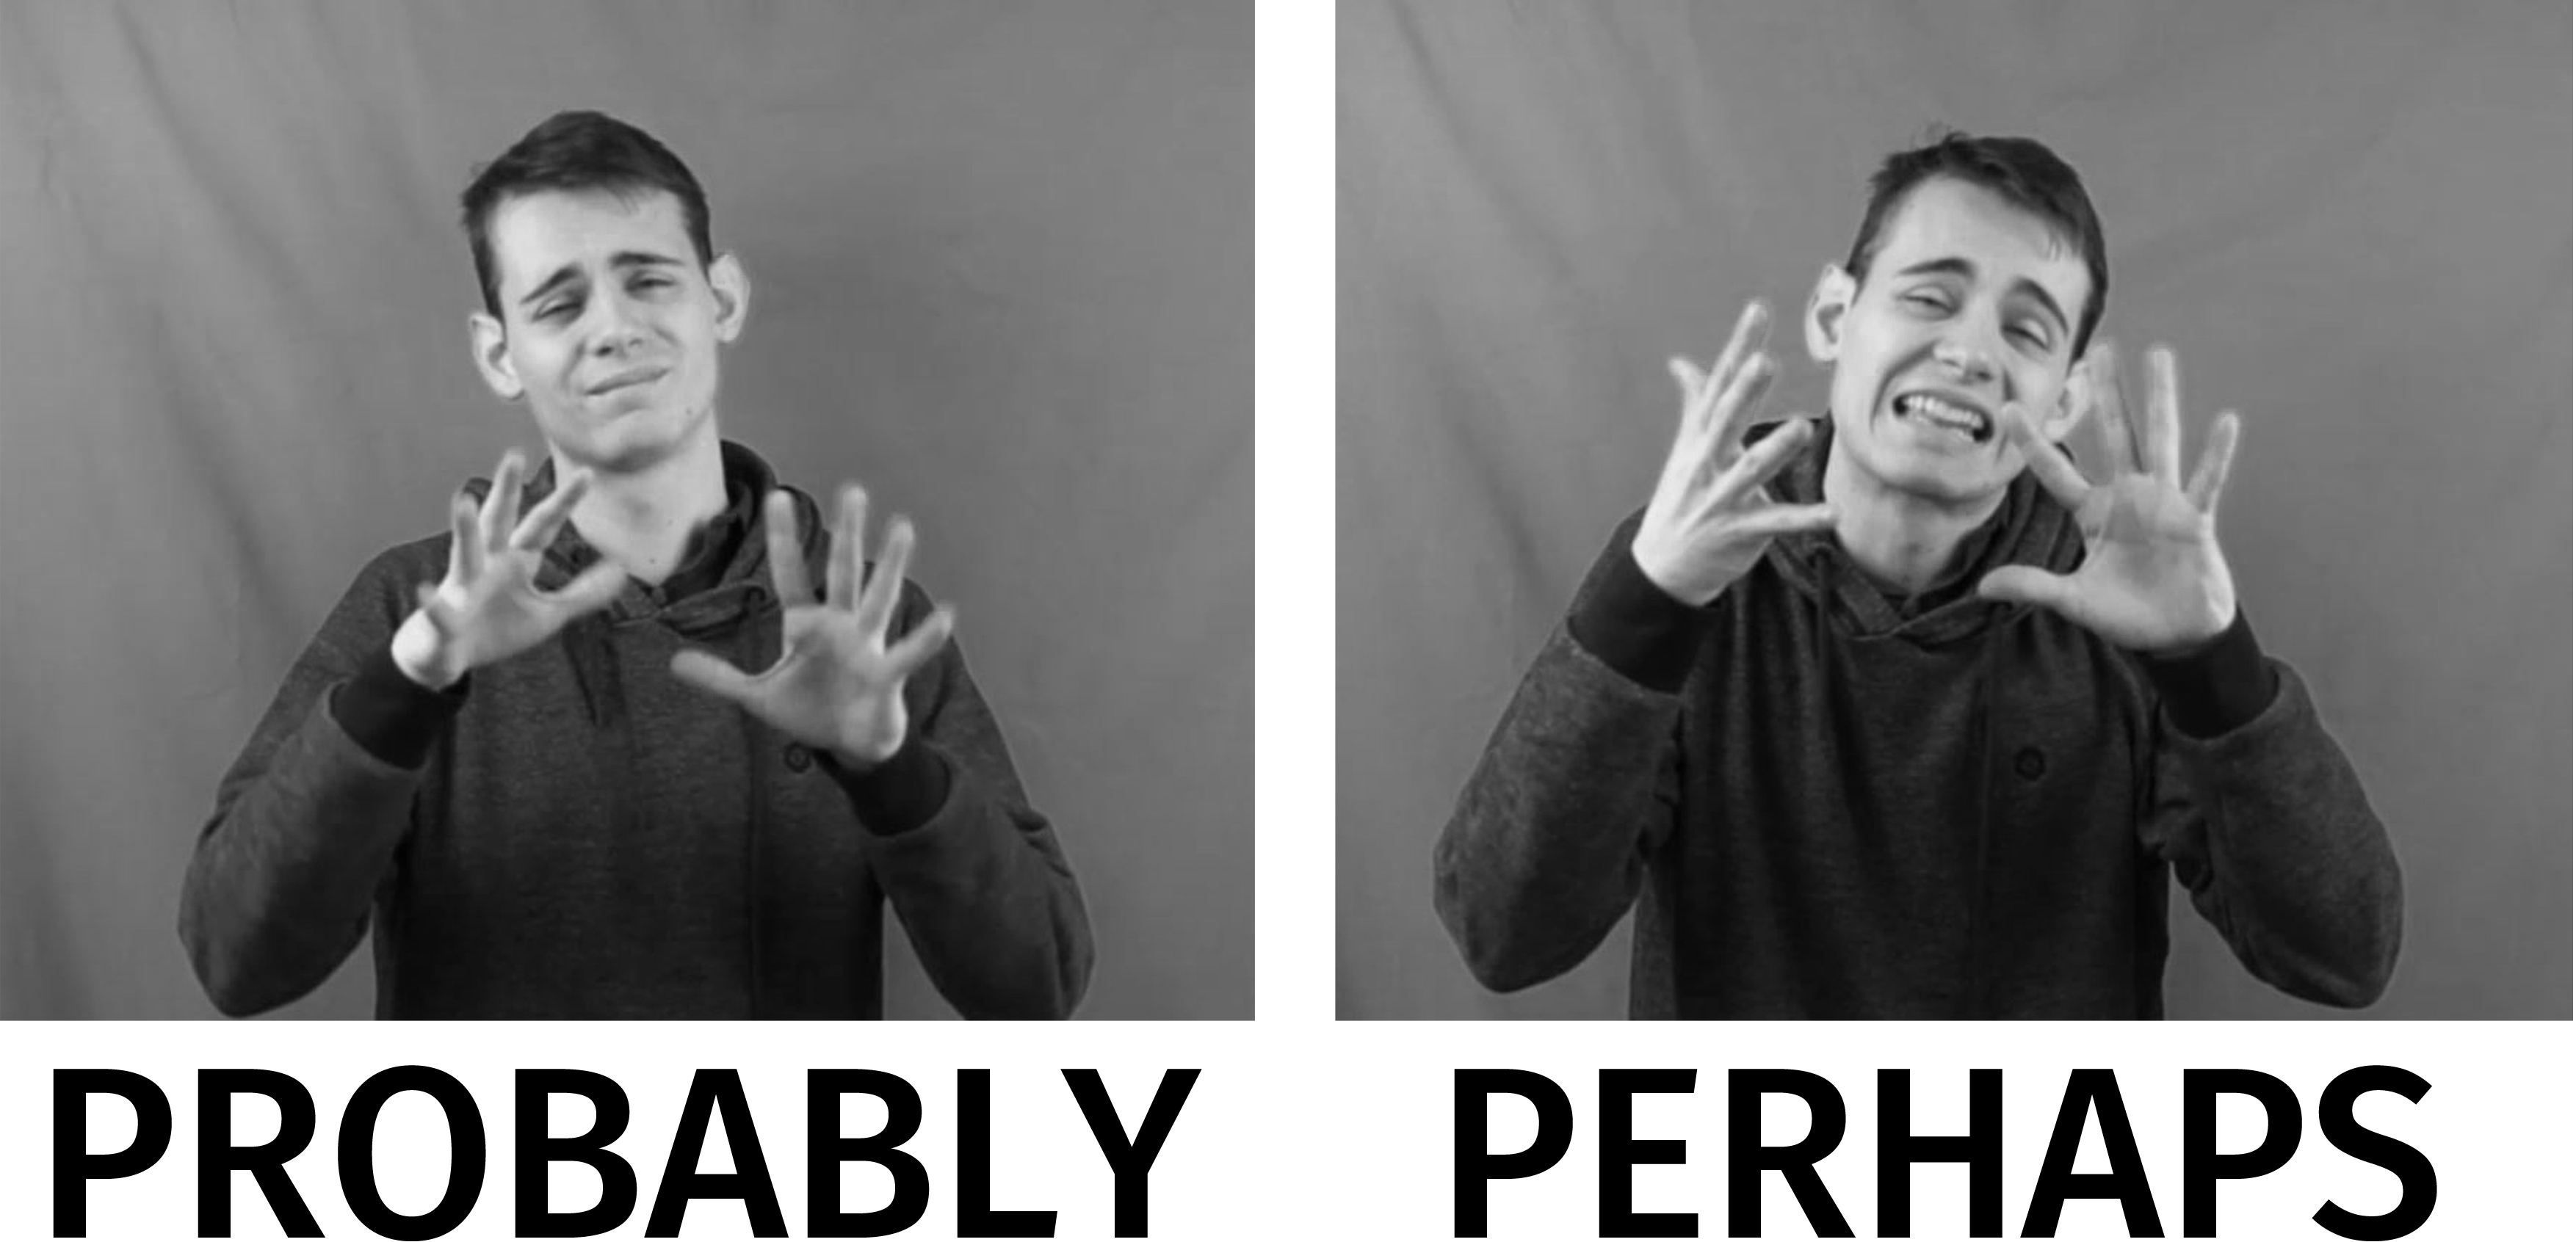
\includegraphics[width=1.0\textwidth]{probablyperhaps2sw.jpg}
	\caption{The signs \textsc{probably} and \textsc{perhaps} only differ in their non-manual markings. With \textsc{probably}, the head is slanted to the side, the eyes are tensed, and the eyebrows are slightly furrowed. The same is true for \textsc{perhaps}, but to a stronger degree. Additionally, with \textsc{perhaps} the torso is put forward (leading to the impression that the sign is executed closer to the face).}
	\label{fig:probablyperhaps}
\end{figure}

The non-manual markings produced with the upper-face are the same in both contexts, i.e., we find the typical brow and eye markings with \textsc{perhaps} as in epistemic contexts (the same is true for \textit{almost certainly} cases). While I take epistemic modality and Cinque's irrealis to belong to the same high category, the generalization regarding the non-manual markings is nevertheless important. The overall generalization is that the more the head is slanted the more insecure the signer is towards the proposition expressed (this is true regardless of whether a manual adverb is used or not). Conversely, the more straight the head position is, the more certain the signer is about the truth-value of the proposition. On the very end of the spectrum a head nod appears (with closed eyes when the source of information is epistemic and with wide-open eyes when the information source is assumed to be shared), as described in Section \ref{evidentiality} and Section \ref{sectionepistemic}.

I conclude this section with the observation that DGS only presents a non-manual difference between the expression of epistemic modality and irrealis mood, at least concerning \textsc{probably} and \textsc{perhaps}, and take the data presented in this section as evidence that the position of what Cinque calls `irrealis' belongs either to epistemic modality or is at least located higher up in the tree. 

\is{irrealis|)}

\section{Alethic modality}\label{alethicmodal}\is{alethic modality|(}
Note that this category was suggested to be located below tense in Cinque's system. I argue, however, that alethic modality is probably not a linguistic category in its own right, but rather coincides with epistemic modality -- or, alternatively, is a category in its own right, but scopes above tense. 

\subsection{General overview}
Below mood irrealis and above habitual aspect, \citet{cinque1999adverbs} locates alethic modality (as already mentioned in Section \ref{introcinque} and \ref{anoteonmodality}). In this Section, I will review the use of the term `alethic' in the literature and argue that it is not a linguistic category, but a special case of epistemic modality. Instead of using Cinque's rather broad definition, I make a more fine-grained distinction of modal flavors (cf. Section \ref{anoteonmodality}). In the position \citet{cinque1999adverbs} locates alethic modality, I locate deontic modality, which will be discussed in Section \ref{deonticmodalsection}.

According to \citet[78]{cinque1999adverbs} alethic modality, a term introduced by \citet{von1951essay},\footnote{ The terms `epistemic', `deontic' and `dynamic' are also from \citet{von1951essay}.} is a modal flavor concerned with

\begin{quote}
the \textit{necessary} truths (i.e., propositions that are true in all possible worlds) and with \textit{possible} truths (i.e., propositions that are \textit{not necessarily false}, being true in at least one possible world). $[$Emphasis in original$]$ %(Cinque 1999:78)
\end{quote}

\noindent While epistemic modality is about the knowledge and the beliefs of an individual, alethic modality is about ``the necessary and contingent truth of propositions'' \citep[8--9]{nuyts2006modality}. Thus, the distinction between epistemic and alethic modality is one between truths in the mind of an individual versus truths in the world (\citealt[11]{palmer1986mood}; \citealt[9]{nuyts2006modality}). A clear case of alethic necessity is something like \textit{Two and two must be four}, because this statement is true by definition and therefore true in all possible worlds. It is, however, not exactly clear if such statements are truly independent of the beliefs of an individual, which seems, in my mind, to be impossible, even in the case of apodeictic statements (e.g., \textit{a square must have corners}). Concerning the linguistic expression of alethic modality, many authors, most prominently \citet[11]{palmer1986mood}, assume that alethic modality is not a linguistic, but rather a logical category and speculate that there may be no language that makes a formal grammatical distinction between epistemic and alethic modality (see also \citealt[28]{nuyts2000epistemic} and \citealt{von2006modality}).

While I would tend to follow this line of reasoning and argue that alethic and epistemic modality are either the very same category or at least very similar (and thus should both scope above tense), a more problematic reason why I believe that Cinque's reasoning that alethic modality scopes below tense is not correct is that his examples only include alethic possibility which is, according to him, about ``\textit{possible} truths (i.e., propositions that are \textit{not necessarily false}, being true in at least one world)''. Such a broad definition would subsume sentences like \textit{Paris Hilton can do one hundred push-ups} since there should be one world in which this proposition is true. I think it is more reasonable to define alethic modality as the modality of necessary truths (as, for example in \citealt{nuyts2000epistemic}) and rule out alethic possibility -- otherwise too many instances of possibility (including, for example, irrealis mood) have to be subsumed under this label. 

Cinque bases his arguments that alethic modality scopes below tense only on alethic possibility. His starting points are facts from English multi-modal constructions that are possible in some varieties, e.g. in Hawick Scots as shown in (\ref{bsp:multimodalenglish}). 

\begin{exe}
\ex\label{bsp:multimodalenglish} 
Hawick Scots \citep[75]{brown1922double}  \\He'll might could do it for you ($=$ `he might be able in the future to do it for you').
\end{exe}

\noindent In this case, Cinque argues, that one can see that the alethic modal \textit{might} follows the future marker \textit{will} while epistemic markers usually precede future markers. In contrast to Cinque, I would argue, however, that \textit{might} in this case does not express alethic, but epistemic modality. To be more precise, it indicates that the speaker makes a guess (based on what he knows about the referent) about the likelihood of an event to occur (see \citealt[6]{bour2014description} for a similar line of reasoning).  ``A comparable situation is found in Danish'', \citet[79]{cinque1999adverbs} continues. He then cites the following two examples from \citet[10]{vikner1988modality}:

\begin{exe} 
\ex Danish \citep[10]{vikner1988modality}\begin{xlist} 
\ex \label{bsp:vikner1988a} 
\textcolor{white}{*}Der vil let kunne g\aa\ noget galt.%$\mathring{\textrm{a}}$
\trans \textcolor{white}{*}`It will easily be possible that something goes wrong.'
\ex\label{bsp:vikner1988b}
*Han vil skulle have l\ae st bogen.
\trans \textcolor{white}{*}`He will be said to (must) have read the book.'
\end{xlist} 
\end{exe}

\noindent According to \citet[79]{cinque1999adverbs}, ``the alethic modal \textit{kunne}, but not the epistemic/evidential modal \textit{skulle}, can be found following the modal \textit{vil} marking the future.'' However, \citet[10]{vikner1988modality} discusses his examples as cases of the ``combination of two epistemic'' modals, namely epistemic \textit{vil} and epistemic \textit{kunne}/\textit{skulle}. He actually does not talk about alethic modality -- and I think that the examples above do not involve alethic modality as it is not clear to me if alethic possibility exists at all.\footnote{ Although I do think that alethic impossiblity exists. Examples include \textit{A square cannot have corners} or \textit{I might never have been born}. The latter example is from \citep[16]{kroeger2018} who notes: ``It is possible for me to imagine states of affairs in which I would not exist [\dots ]; but none of these states of affairs are epistemically possible, because they are inconsistent with what I know about the real world.''}

\subsection{The situation in DGS}
Turning back to DGS, manual modals are disallowed in alethic contexts in German Sign Language, just as in epistemic contexts. The example in (\ref{ex:alethic}) shows that the expression of alethic modality is very similar to, if not indistinguishable from, epistemic modality. This can be seen from the comparison of alethic (\ref{alethica}) with epistemic contexts (\ref{alethicb}). Note that in both contexts, closing the eyes on the verb sign could be added, indicating that the signer is very sure about the proposition expressed. The nod serves as an additional certainty/focus marker.




\begin{exe}
\ex\label{ex:alethic}\begin{xlist}
\ex \slgl[furrowed brows]{two\textsubscript{\textup{left}} two\textsubscript{\textup{right}} \slg[\textup{nod}]{four}}
\glt `Two and two must be four.' \label{alethica}\hfill{\textit{Alethic modality}}
\ex  \slgl[furrowed brows]{paul \slg[\textup{nod}]{at-home}}
\glt `Paul must be at home.' \label{alethicb}\hfill{\textit{Epistemic modality}}
\end{xlist}
\end{exe}





\noindent In most cases, however, statements of the form \textit{Two and two must be four} were translated as \textit{Two and two equals four} with a focus marker on the predicative expression. To conclude this section, the expression of alethic and epistemic modality is, as predicted by cross-linguistic research, indistinguishable in DGS. 


\is{alethic modality|)}

The next lower category that also represents the last category above tense will be the first that does not show non-manual marking with the upper face and presents a different spreading behavior.

\section{Scalarity (\textit{little}/\textit{much})}\label{scalarity}\is{scalarity|(}

\subsection{General overview}
The projection labeled `scalarity' is concerned with the speaker's evaluation of something as being little or much. The syntactic position of the scalarity projection is argued to be above Tense and below epistemic modality in \citeauthor{hole2015distributed} (\citeyear{hole2015distributed}, \citeyear{hole2017crosslinguistic}) and in \citet{bross2017scope}. The evaluation of something as being little/much and something as being good/bad often goes hand in hand, as the example in (\ref{beispielelf}) illustrates (from \citealt[51]{hole2015distributed}).

\begin{exe} 
\ex \textit{Paul only eats cookies.} \\ `Paul eats nothing apart from cookies.' \label{beispielelf} 
\begin{xlist} 
\ex possible evaluation as `little': eating nothing but cookies is considered little by the speaker\label{beispielelfa}
\ex possible evaluation as `bad': eating nothing but cookies is considered bad by the speaker \label{beispielelfb} 
\ex possible evaluation as `bad' and `little': eating nothing but cookies is considered bad and little by the speaker \label{beispielelfc} 
\end{xlist} 
\end{exe}

\noindent The sentence in (\ref{beispielelf}) has the at-issue meaning that Paul eats nothing apart from cookies, i.e., an exclusive reading. However, there are several not-at-issue evaluations that this sentence, depending on intonation and context, can have. These are shown in (\ref{beispielelfa}), (\ref{beispielelfb}), and (\ref{beispielelfc}). The crucial reading intended here is the evaluation as little (\ref{beispielelfa}).

\subsection{The situation in DGS}
In DGS, when something is evaluated as little, the cheeks are sucked-in or are pressed and small. When something is evaluated as much, the cheeks are puffed for a short moment, then the air is released. Sucking in or puffing the cheeks is restricted to the predicate and cannot accompany the whole clause. This is shown in the examples in (\ref{bsp:evaluationmuchlittle}) with `() ()' indicating puffed cheeks and `)( )(' indicating sucked-in cheeks.

\begin{exe}
\ex\label{bsp:evaluationmuchlittle}\begin{xlist}
\ex 
{\textsc{paul three book+++ write}}   
\glt `Paul has written three books.'\label{bsp:evaluationmuchlittlea}
\ex \slg{paul three book+++} \slg[() ()]{write}
\glt `Paul has written three books (and I evaluate this as much).'\label{bsp:evaluationmuchlittleb}
\ex \slg{paul three book+++} \slg[)( )(]{write}
\glt `Paul has written three books (and I evaluate this as little).'\label{bsp:evaluationmuchlittlec}
\end{xlist}
\end{exe} 


\begin{figure}[bt]
\centering
	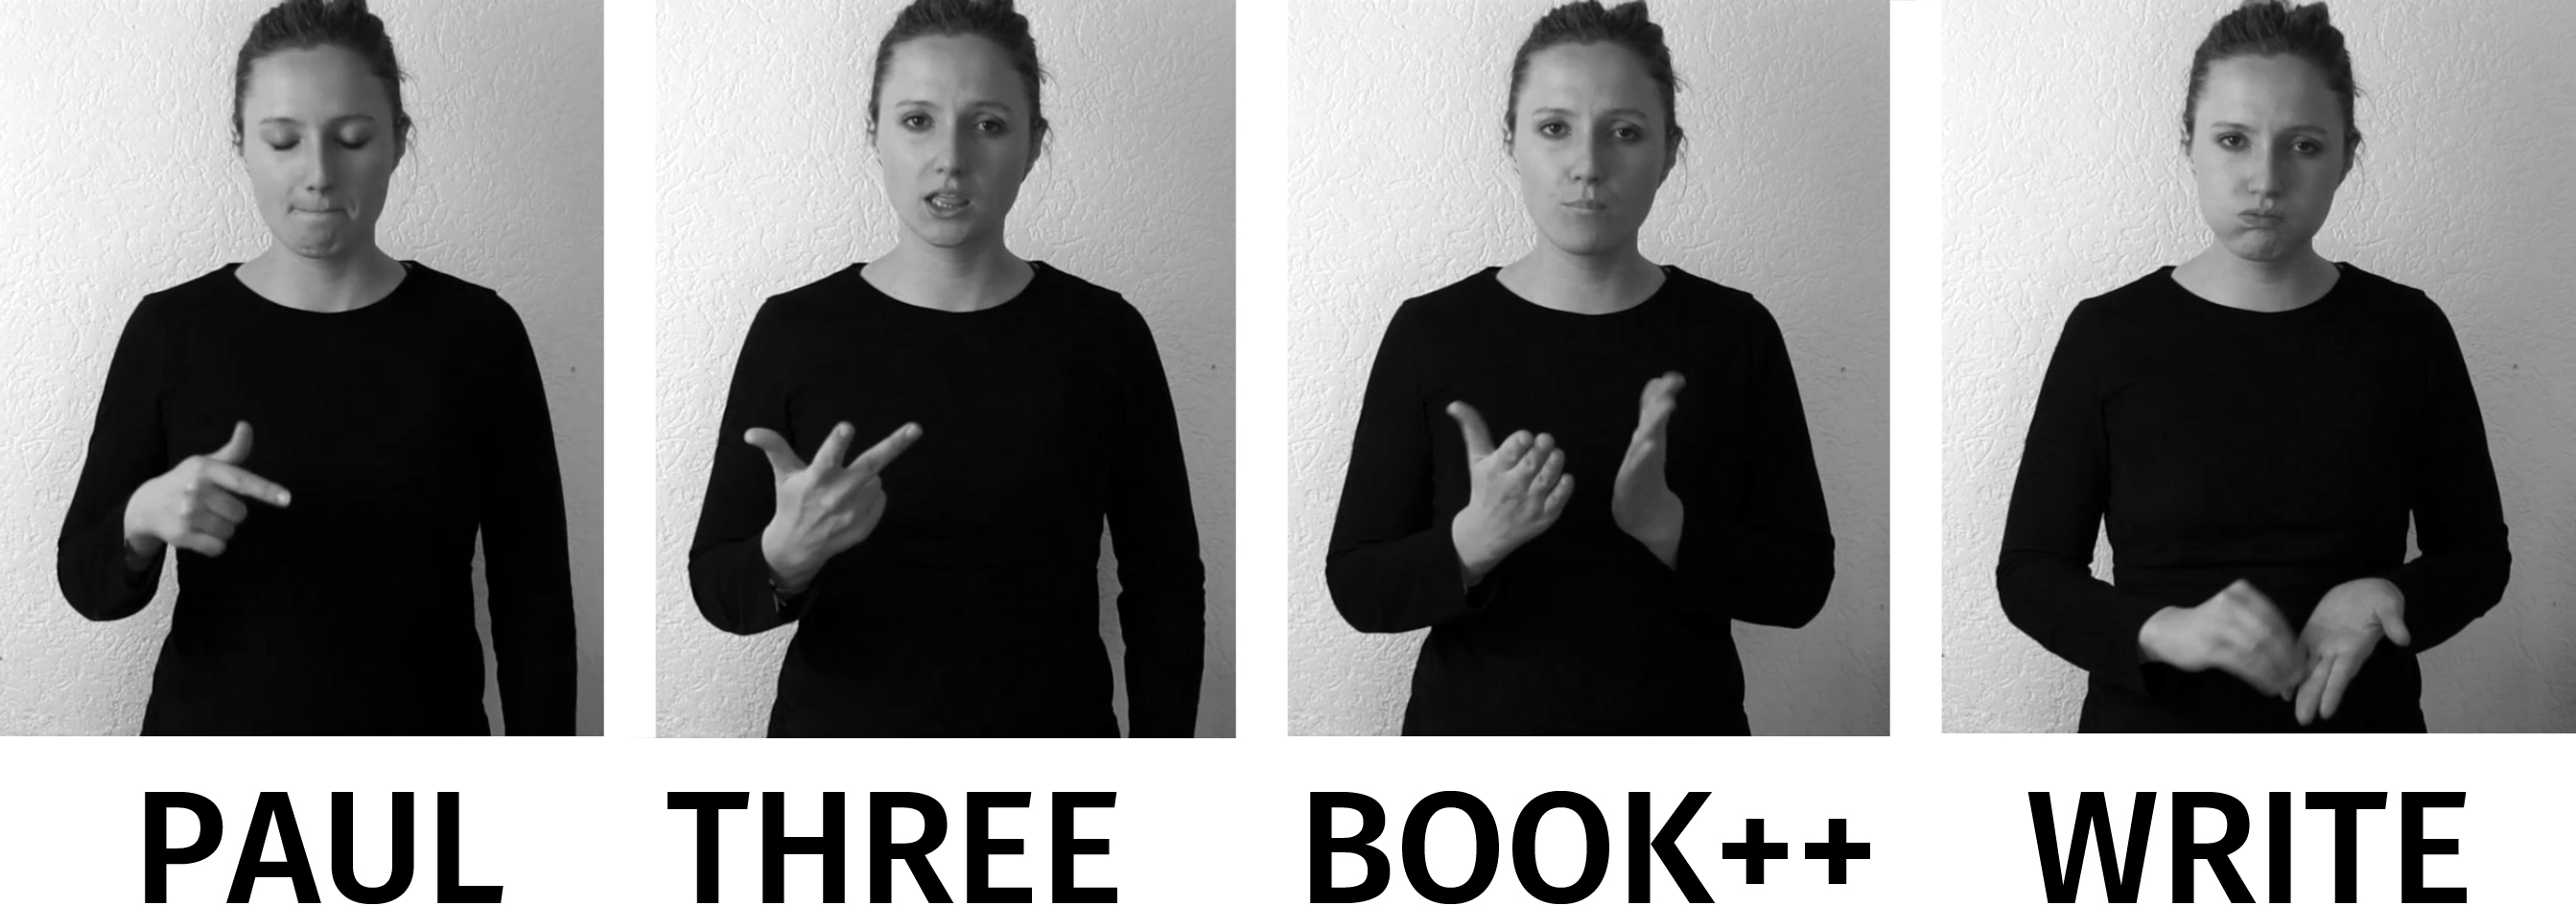
\includegraphics[width=1.0\textwidth]{evalmuchsw.jpg}
	\caption{Evaluation as being much. This type of scalarity is expressed non-manually by puffed cheeks.}
	\label{fig:evalgood}
\end{figure}

\noindent The neutral sentence in (\ref{bsp:evaluationmuchlittlea}) serves as a comparative example. When the same sentence is signed with puffed cheecks on the verb (\ref{bsp:evaluationmuchlittleb}) the sentence's interpretation changes insofar as the signer now evaluates the fact that Paul has written three books as much. This sentence is additionally depicted in Figure \ref{fig:evalgood}. The example in (\ref{bsp:evaluationmuchlittlec}) shows the same for the evaluation as being little. Note that it has been reported for some sign languages that puffed cheeks can also accompany noun signs. \citet[102--103]{boyesbram1990gebaerdesprache}, for example, reports that puffed cheeks may accompany the noun sign \textsc{cake} meaning `much' or `lots of' in \is{Swiss German Sign Language}Swiss German Sign Language (see \citealt{bakerpfau2016} for similar claims for \is{Sign Language of the Netherlands}Sign Language of the Netherlands and \is{British Sign Language}British Sign Language). This, however, is not possible in DGS as both puffed and sucked-in cheeks/pressed lips are only allowed to accompany the verb and, in some cases, adverbs (see, for example, Section \ref{justjust}).\footnote{ Exceptions include lexical non-manuals of some nouns.}

Instead of sucked-in cheeks, tensed lips, sometimes with a tongue protrusion can be observed in some contexts. In some cases, the tongue protrusion is missing. The exact meaning differences between these similar, but distinct non-manuals have to be worked out in future research. 

As with the other high categories discussed so far, it is possible to add a manual adverb in scalarity contexts. In this case, the adverb must appear pre-verbally, but is not allowed in a clause-initial position. An example is given in (\ref{bsp:shortvisitpaul}). In this case, we observe pressed lips to evaluate that Paul visiting only for a short time is (only) little. Pressed lips are glossed `$==$' in the example.

\begin{exe}
\ex \slg{paul always briefly} \slg[$==$]{visit}
\glt `Paul always visits only briefly.'\label{bsp:shortvisitpaul}
\end{exe}

\noindent Before concluding this section, I will briefly discuss one final example that was originally elicited in the context of generic aspect discussed in Section \ref{characteristic}. The sentences labeled 1 (on the left) and 2 (on the right) of Figure \ref{fig:littlemuchlion} both mean \textit{The lion became extinct}. The difference between the examples is expressed via the mouth region. In the first example, with the cheeks puffed on the verb there is the additional evaluation that there were many lions left that became extinct. In the second example, there is the additional evaluation that there were only a small number of lions left that went extinct. 

\begin{figure}[bt]
\centering
	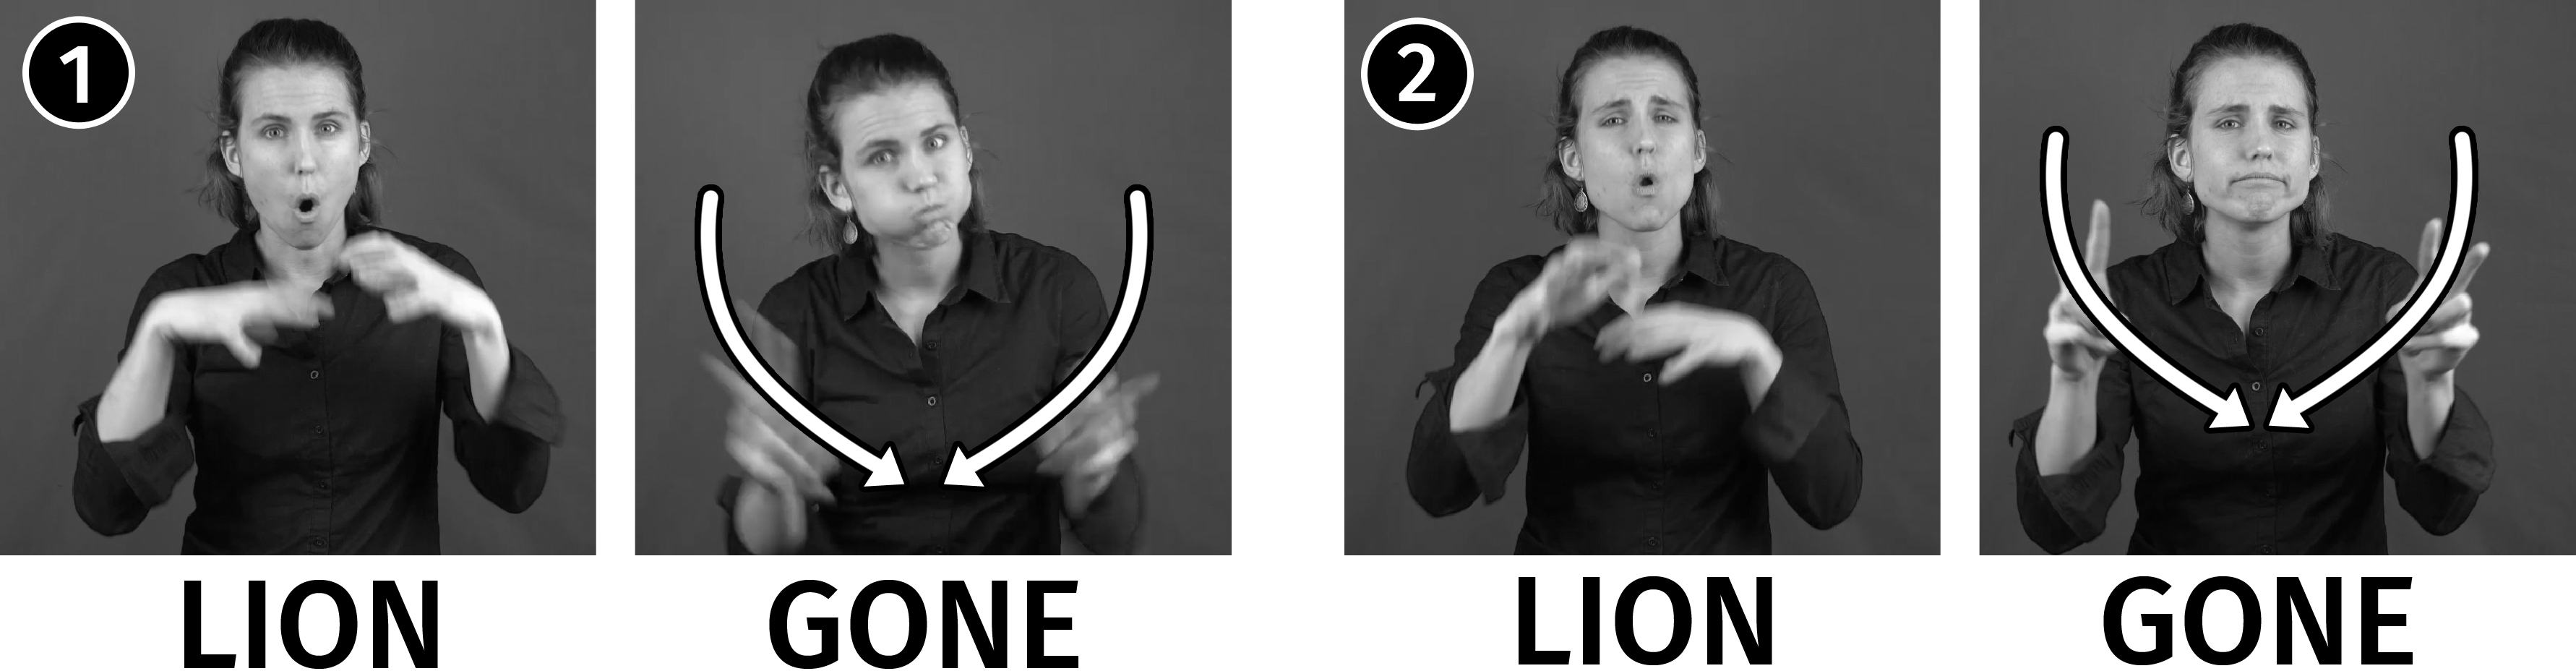
\includegraphics[width=1.0\textwidth]{littlemuchlion2sw.jpg}
	\caption{Two versions of \textit{The lion went extinct}. The example labeled 1 has the additional meaning that there were many lions that went extinct; the example labeled 2 has the additional meaning that there was only a small amount of lions left.}
	\label{fig:littlemuchlion}
\end{figure}

In conclusion, scalarity is a high category above tense that can be expressed via non-manual marking only or by a combination of a manual pre-verbal adverb and the respective non-manual marker. The spread of the non-manual markers is comparably small as they only appear on the verb sign. The crucial point is that the high categories were presented in descending order and that for expression of scalarity a lower body-part is used than for the categories higher up in the structure. 

I will now briefly summarize the observations for the higher categories made so far and draw some conclusions relating to the clause structure of DGS. Then I will discuss the differences between non-manual and manual markers concerning their at-issueness and will then proceed to discuss the next lower category, namely Tense.
\is{scalarity|)}
\section{Interim summary: high categories and non-manual expressions}
\largerpage

The previous chapter and the preceding sections in this chapter have shown that all the structurally high categories, i.e., all categories above Tense, are expressed non-manually. For the Cinquean categories above Tense, it turned out that DGS can switch between a manual/non-manual and a non-manual-only strategy. This is in line with observations found in the literature: \citet[365--366]{happ2014vork} mention that the sentential adverbs \textit{hopefully}, \textit{fortunately}, \textit{unfortunately}, \textit{stupidly}, \textit{cleverly}, \textit{annoyingly}, \textit{kindly}, and \textit{interestingly} all receive special non-manual markings spreading over the whole clause (see also \citealt{herrmann2014nonmanual}). These are, crucially, all higher \is{speaker-oriented adverbs}speaker-oriented adverbs. However, they do not mention that these adverbs can also be expressed non-manually only.

When the manual strategy is chosen for the high Cinquean categories, the non-manuals still obligatorily spread over the clause, but with reduced intensity. For the high CP categories (i.e., those located above speech-act-indicating expressions), given that the non-manuals accompanied the whole clause, the spread of the non-manuals `started' from a clause-final position.

For the Cinquean categories, the intensity peak of the non-manuals is clause-initial -- with two exceptions: when there is no evidential adverb, an additional sideways inclination of the head was observed on the verb in \textit{allegedly} contexts, i.e., in a clause-final position. See also the discussion of this kind of head inclination in Section \ref{perhapsmoodirrealis}. Crucially, however, the non-manual markers produced with the eyebrows still had their intensity peak clause-initially. Additionally, non-manuals used in scalarity contexts do not have their intensity peak clause-initially because the non-manuals do not spread over the whole clause.

The hypothesis that high categories receive non-manual markings with a high body part was generally confirmed. To be more precise, all the \is{speaker-oriented adverbs}speaker-oriented categories above Tense, shown in (\ref{bsp:highcategories}), receive non-manual markings (the main non-manual markers are given on the right). Additionally, scalarity marking is the turning point at which the non-manuals are no longer produced with the eyebrows/eyes, but with a lower body part, namely the cheeks. At the same time, with this category, the spread of the non-manuals is no longer over the whole clause, but only over the predicate.

\begin{exe}
\ex\label{bsp:highcategories} 
\begin{adjustbox}{max width=0.9\textwidth}
\begin{tabular}[t]{p{3.2cm}p{2.8cm}p{2.6cm}p{2.5cm}} %11.6 13
\textsc{Category} & \textsc{Scopal domain} & \textsc{Onset} & \textsc{Articulator}  \\
Mood\textsubscript{speech act} & clause & clause-initial & brows \\
\textcolor{white}{nn}Mood\textsubscript{mirative} & clause & clause-initial & brows, eyes\\
\textcolor{white}{nnn}Mood\textsubscript{evaluative} & clause & clause-initial & brows, eyes \\
\textcolor{white}{nnnn}Mood\textsubscript{evidential} & clause & clause-initial & brows, eyes \\
\textcolor{white}{nnnnn}Mod\textsubscript{epistemic} & clause & clause-initial & brows, eyes \\
\textcolor{white}{nnnnnn}Mod\textsubscript{scalarity} & predicate & predicate onset & cheeks \\
\end{tabular}
\end{adjustbox}
\end{exe}

\noindent Of course, one has to keep in mind that the non-manual markers used for each category consist of complex bundles and it is often difficult to disentangle the meaning contribution of each part. It has been proposed that non-manuals combine in a compositional way with each marker (e.g., wide-open eyes or brow-raise) contributing one semantic feature (e.g., \citealt{herrmann2013modal}). This is an attractive hypothesis, especially from the point of view of nano-syntax that is desperately in need of more research. To this hypothesis I add that the position of the respective syntactic head also plays a crucial role in semantic interpretation. This can be best illustrated for mirativity as the non-manuals used in mirative constructions seem to be indistinguishable from the ones used in polar interrogatives, the only difference being the intensity peak of the non-manuals. 

If the hypothesis that the intensity peak of the non-manuals reflects the location of their respective syntactic heads is correct, the categories in (\ref{bsp:highcategories}) are left-headed. This is also true for scalarity although scalar adverbs do not appear clause-initially, but rather pre-verbally. As all the adverbs (with the exception of scalarity) are clause-initial, their respective projections can be thought of as being left-branching. Thus, we arrive at a representation as in (\ref{ex:lowercp}). 




\begin{exe}
\ex \label{ex:lowercp}
\resizebox{.9\textwidth}{!}{
\begin{forest}
for tree={s sep=3.8mm, inner sep=0, l=10mm} %s sep = Breite; l = Höhe
[SpeechActP [{\phantom{NNN}} ] [{$\overline{\textrm{SpeechAct}}$} [{SpeechAct\textdegree } ] [MirativeP [.{\phantom{NNN}} ] [{$\overline{\textrm{Mirative}}$} [{Mirative\textdegree } ] [EvaluativeP [{\phantom{NNN}} ] [{$\overline{\textrm{Evaluative}}$} [{Evaluative\textdegree } ] [EvidentialP [{\phantom{NNN}} ] [{$\overline{\textrm{Evidential}}$} [{Evidential\textdegree } ] [EpistemicP [{\phantom{NNN}} ] [{$\overline{\textrm{Epistemic}}$} [{Epistemic\textdegree } ] [ScalarityP [.{\phantom{NNN}} ] [{$\overline{\textrm{Scalarity}}$} [{Scalarity\textdegree }] [{\phantom{NNN}},edge=dashed] ] ] ] ] ] ] ] ] ] ] ] ]
\end{forest}
}
\end{exe}


%\begin{exe}
%\ex \label{ex:lowercp}
%\begin{adjustbox}{max width=0.9\textwidth}
%
%\begin{tikzpicture}[baseline=(current bounding box.north), scale=1.00]
%\tikzset{level distance = 30pt ,sibling distance=1pt}
%\tikzset{every tree node/.style={align=left,anchor=north}}
%\Tree [.SpeechActP [.{} ] [.{$\overline{\textrm{SpeechAct}}$} [.{SpeechAct\textdegree } ] [.MirativeP [.{} ] [.{$\overline{\textrm{Mirative}}$} [.{Mirative\textdegree } ] [.EvaluativeP [.{} ] [.{$\overline{\textrm{Evaluative}}$} [.{Evaluative\textdegree } ] [.EvidentialP [.{} ] [.{$\overline{\textrm{Evidential}}$} [.{Evidential\textdegree } ] [.EpistemicP [.{} ] [.{$\overline{\textrm{Epistemic}}$} [.{Epistemic\textdegree } ] [.ScalarityP [.{} ] [.{$\overline{\textrm{Scalarity}}$} {Scalarity\textdegree } \edge[dashed]; {} ] ] ] ] ] ] ] ] ] ] ] ]
%%\Tree [.NP [.SpecNP ] [.{$\overline{\mathrm{N}}$} [.Adj cute ] [.{$\overline{\mathrm{N}}$} [.Adj tiny ] [.{$\overline{\mathrm{N}}$} [.{N\textdegree} kitten ] [.{} ] ] ] ] ]
%\end{tikzpicture}
%\end{adjustbox}
%\end{exe}

One point that has not been discussed so far is the question of what happens when several categories requiring different non-manual markings are combined. Although I did not look systematically at this question, it seems that the combination of two lower CP categories requires the insertion of manual signs. An example is given in (\ref{combinationofmarkers}). 

\begin{exe}
\ex\label{combinationofmarkers}\begin{xlist}
\ex \textcolor{white}{*}\slgl[mirative]{surprisingly paul} \slgl[evaluation: bad]{unfortunately there girlfriend}
\glt \textcolor{white}{*}`Surprisingly, Paul unfortunately has a girlfriend.'\label{combinationofmarkersa}
\ex *\slgl[evaluation: bad]{unfortunately paul} \slgl[mirative]{surprisingly there girlfriend}
\glt \textcolor{white}{*}Intended: `Surprisingly, Paul unfortunately has a girlfriend.'\label{combinationofmarkersb}
\end{xlist}
\end{exe}

\noindent The data in (\ref{combinationofmarkers}) shows that DGS follows a pattern also found in English or German: The structurally higher adverb appears in a clause-initial position while the structurally lower one follows the subject. As predicted, the order of the adverbs is fixed, as evidenced by the illformedness of example (\ref{combinationofmarkersb}). Additionally, the non-manual markings related to the higher adverb do not only spread over the adverb, but also over the subject. One interesting assumption would be that the subject has moved into some structurally higher position, but I will leave this question for future research too.

In the next section, I will discuss the different meaning contributions of the manual and non-manual expression of the categories discussed so far. Then, I will go on to discuss Tense and the categories below it.

%\clearpage



\section{The at-issue/not-at-issue divide}\label{atnotissue}\is{at-issue meaning|(}\is{not-at-issue meaning|see{at-issue meaning}}
As already briefly mentioned in Section \ref{hypotheses}, introducing the main hypothesis of the present work, \citet{bross2017scope} claim that higher categories which find non-manual expression contribute not-at-issue meaning while manual material contributes at-issue meaning. More broadly speaking, this implies that the at-issue/not-at-issue divide is built into the syntactic tree: categories above IP/TP express not-at-issue meaning while categories below IP/TP express at-issue meaning. In this section, I will briefly discuss the notion of `at-issueness' and show that this claim essentially seems to be true.

\subsection{General overview}
Traditionally, semantics is the linguistic discipline addressing the meaning of morphemes, words, and sentences. The meaning of a sentence is usually modeled by truth values -- an idea going back at least to Gottlob Frege and Ludwig Wittgenstein. According to \citet{wittgenstein1922trac}, understanding the meaning of a sentence means to understand what the world should look like in order for the sentence to be true. In Wittgenstein's words:

\begin{quote}
To understand a proposition means to know what is the case, if it is true. (One can therefore understand it without knowing whether it is true or not.) One understands it if one understands its constituent parts. (Tractatus Logico-Philosophicus, 4.024).
\end{quote} 

\noindent In this kind of truth-functional semantics, understanding a sentence like \textit{The cat drank my beer} thus means to know in what type of world this sentence would be true (i.e., a world in which there is a certain cat we were talking about that drank a beer that was in the speaker's possession). For this, in Wittgenstein's view, it does not matter if the sentence is actually false. 

Truth-functional semantics, however, cannot model all types of meanings. The reason for this is that there are meanings which are not relevant for truth-values. Obviously, many words, expressions, and constructions do contribute directly to truth-values. We can show that an expression contributes to the truth-value of a sentence by trying to refute the truth-value contribution of the expression. This is shown in (\ref{catbeeratissuda}). As mentioned, there are expressions that do not contribute meaning in this way. In these cases, refuting the meaning contribution of the expression fails, as shown in (\ref{catbeeratissudb}). 

\begin{exe}
\ex\label{catbeeratissud}\begin{xlist}
\ex A: \textcolor{white}{\#}That bastard cat drank my beer.  \\
B: \textcolor{white}{\#}That's not true! It was the dog who drank the beer.\label{catbeeratissuda}
\ex A: \textcolor{white}{\#}That bastard cat drank my beer.  \\
B: {\#}That's not true! You like the cat.\label{catbeeratissudb}
\end{xlist}
\end{exe}

\noindent In example (\ref{catbeeratissuda}), Bob successfully refutes the truth-value of Alice's sentence. This works as the word \textit{cat} directly contributes to the truth-value of the sentence. We call this type of meaning which directly contributes to truth-conditional content `at-issue meaning'. In example (\ref{catbeeratissudb}) Bob attempts to refute Alice's evaluation of the cat as a bastard. While we clearly understand that Alice does not like the cat from her utterance in (\ref{catbeeratissudb}), this kind of (expressive) meaning cannot be refuted in the same way. This kind of meaning which contributes non-truth-conditional content is called `non-at-issue meaning' (see, for example, \citealt{karttunen1973presuppositions, simons2010projects, tonhauser2013toward, gutzmann2015use, potts2005logic}).\footnote{ Note that refuting the truth-value of a sentence is only one of many tests of (not-)at-issueness. In fact, there is a whole battery of such tests, called `family of sentences tests' (for an overview see \citealt{potts2005logic}).} Sometimes the terms `truth-conditional meaning' and `use-conditional meaning' are used instead (e.g., \citealt{gutzmann2015use}).

Applying the truth-value refutation test to categories of different heights on the Cinquean hierarchy reveals that the categories above T in general contribute not-at-issue meaning while the categories below T contribute at-issue meaning \citep{bross2017scope}. This can be illustrated using English examples. The mini dialogues in (\ref{goodandbaddiscoursea}), partially adapted from \citep[10]{bross2017scope}, illustrate that it is not possible to refute the meaning contributions of the categories above T, namely speech acts themselves (\ref{goodandbaddiscoursezweo}), speech-act indicating operators (\ref{goodandbaddiscoursea}), evaluation (\ref{goodandbaddiscourseb}), epistemicity (\ref{goodandbaddiscoursec}), and scalarity (\ref{goodandbaddiscoursed}). The same test, however, works for categories below T, as exemplarily shown for volition (\ref{goodandbaddiscourseehans}), deontic modality (\ref{goodandbaddiscourseehansensbeispiel}), prospective aspect (\ref{goodandbaddiscourseehansensbeispielb}), and root modality (\ref{goodandbaddiscourseg}).

\begin{exe}
\ex\label{goodandbaddiscourse}
\begin{xlist}
						\ex Speech-acts \label{goodandbaddiscoursezweo} \\
								A: \textcolor{white}{\#}Is Paul drinking beer? \\
								B: \#That's not true. You're not asking a question.
								\ex Speech-act-indicating operators \label{goodandbaddiscoursea} \\
								A: Honestly, I did not read the book. \\
								B: That's not true. \#That's not honest.
								 \ex Evaluation as good or bad \label{goodandbaddiscourseb}\\
								A: Luckily, Paula is at home. \\
								B: That's not true. \#It's unfortunate that she is at home.
						\ex Epistemic modality \label{goodandbaddiscoursec}\\
								A: The light is on. Markus must be at home. \\
								B: That's not true. \#You have first-hand knowledge that he is \\
								\textcolor{white}{A: }at home!
						\ex Scalarity (evaluation as much or little) \label{goodandbaddiscoursed} \\
								A: Paula eats only salad. \label{goodandbaddiscoursee} \\
								B: That's not true. \#I think for her to eat salad is a lot!
								%\hline
						\ex Volition \\
								A: Paul wants to learn sign language. \label{goodandbaddiscourseehans}\\
								B: That's not true. They force him to learn it.
            \ex Deontic modality$_{\textrm{MUST/CAN}}$ \label{goodandbaddiscourseehansensbeispiel} \\
								A: Paula must tidy up. \\
								B: That's not true. Her parents explicitly said they would do it.\\
								\textcolor{white}{A: }She simply wanted to do it.
						\ex Prospective Aspect \label{goodandbaddiscourseehansensbeispielb} \\
								A: They almost destroyed the city. \\
								B: That's not true. They completely destroyed the city.
						\ex Root modality$_{\textrm{CAN}}$ \label{goodandbaddiscourseg} \\
								A: Paula can perform magic. \\
								B: That's not true. She's a Muggle and has no magical powers.
\end{xlist}
\end{exe}

%\begin{exe}
%\ex \label{goodandbaddiscourse}\begin{xlist}
						%\ex Speech-acts \label{goodandbaddiscoursezweo} \\
								%A: \textcolor{white}{\#}Is Paul drinking beer? \\
								%B: \#That's not true. You're not asking a question.
						%\ex Speech-act-indicating operators \label{goodandbaddiscoursea} \\
								%A: Honestly, I did not read the book. \\
								%B: That's not true. \#That's not honest.
            %\ex Evaluation as good or bad \label{goodandbaddiscourseb}\\
								%A: Luckily, Paula is at home. \\
								%B: That's not true. \#It's unfortunate that she is at home.
						%\ex Epistemic modality \label{goodandbaddiscoursec}\\
								%A: The light is on. Markus must be at home. \\
								%B: That's not true. \#You have first-hand knowledge that he is at home!
						%\ex Scalarity (evaluation as much or little) \label{goodandbaddiscoursed} \\
								%A: Paula eats only salad. \label{goodandbaddiscoursee} \\
								%B: That's not true. \#I think for her to eat salad is a lot!
								%\hline
						%\ex Volition \\
								%A: Paul wants to learn sign language. \label{goodandbaddiscourseehans}\\
								%B: That's not true. They force him to learn it.
            %\ex Deontic modality$_{\text{MUST/CAN}}$ \label{goodandbaddiscourseehansensbeispiel} \\
								%A: Paula must tidy up. \\
								%B: That's not true. Her parents explicitly said they would do it. She simply wanted to do it.
						%\ex Prospective Aspect \label{goodandbaddiscourseehansensbeispielb} \\
								%A: They almost destroyed the city. \\
								%B: That's not true. They completely destroyed the city.
						%\ex Root modality$_{\text{CAN}}$ \label{goodandbaddiscourseg} \\
								%A: Paula can perform magic. \\
								%B: That's not true. She's a Muggle and has no magical powers.
%\end{xlist}
%\end{exe}

 
\noindent As shown in the examples, it is not possible to refute the type of speech act a speaker is making (\ref{goodandbaddiscoursezweo}), nor is it possible to refute the content of a speech-act-indicating expression (\ref{goodandbaddiscoursea}). Similarly, speaker's evaluation (\ref{goodandbaddiscourseb}), epistemicity (\ref{goodandbaddiscoursec}), and scalarity cannot be refuted (\ref{goodandbaddiscoursed}). The situation, however, changes with the categories below tense as all categories starting with volition (\ref{goodandbaddiscourseehans}) contribute at-issue meaning.

Based on similar results, \citet{bross2017scope} propose that the at-issue/not-at-issue divide is hard-wired into the syntactic tree with not-at-issue meaning encoded in the categories above T and at-issue meaning below T. This is not only true for English, but seems to be universal. 

Before turning to the discussion of the at-issue/not-at-issue divide in German Sign Language, two notes are in order. The first note concerns epistemic modality (or modality in general) and the second note concerns the fact that not-at-issue meanings can always be made at-issue during the discourse.

The at-issue/not-at-issue divide as presented above is actually a bit simplistic as it turns out that there are categories in natural languages consisting of an at-issue and a not-at-issue part. This is true for epistemic modality, which contributes two different meanings. The first meaning contribution relates to the modal flavor (e.g., epistemic, deontic, root) and the second to the modal force (possibility/necessity). While the example in (\ref{goodandbaddiscoursec}) shows that the modal flavor is not-at-issue, it turns out that the modal force, in contrast, is at-issue (\ref{forceatissue}).

\begin{exe}
\ex \textit{Epistemic modality:}\\ 
A: The light is on. Paul must be at home.\\
B: That's not true. He \textsc{may} be at home.  \label{forceatissue}
\end{exe}

\noindent This shows that the fact that Paul's being at home in the examples in (\ref{goodandbaddiscoursec}) and (\ref{forceatissue}) is regarded as necessary by the speaker is part of the truth-functional meaning of Alice's statement. The fact that she guesses based on her evidence, in contrast, is part of the use-functional meaning and cannot be refuted.\footnote{ An explanation for this is that modals are generated in a position below T and then move to their scope-taking position to receive their meaning (the flavor). As the modal (and hence, its force) is generated below T, this part of the meaning is at-issue, but the meaning contribution above T, the epistemic interpretation, is not-at-issue.}

Finally, note that the question of whether a meaning is at-issue or not-at-issue depends on how a sentence is constructed. This means that a construction conveying a not-at-issue meaning can always be transformed into an at-issue statement. This is illustrated in (\ref{atissuenotatissuetransformationq}). Although the two sentences are made up of the exact same lexical material, they differ in which part of the sentences is at-issue and which is not. 

\begin{exe}
\ex\label{atissuenotatissuetransformationq}\begin{xlist}
\ex Paul, who likes to drink beer, will be at the party. \label{atissuenotatissuetransformationqa}
\ex Paul, who will be at the party, likes to drink beer. \label{atissuenotatissuetransformationqb}
\end{xlist}
\end{exe}

\noindent While (\ref{atissuenotatissuetransformationqa}) is a sentence about Paul going to a party, (\ref{atissuenotatissuetransformationqb}) is a sentence about Paul liking beer. As appositive relative clauses contribute not-at-issue meaning \citet{potts2005logic},\footnote{ In line with the general idea of this section, it seems that appositive relative clauses always receive upper-face markings in sign languages (see \citealt{pfau2005relative} for DGS and \citealt{branchinidonati2007} and \citealt{wilbur2017internally} for a typological overview).} Paul's liking beer in (\ref{atissuenotatissuetransformationqa}) is not-at-issue. What is at-issue in (\ref{atissuenotatissuetransformationb}) is that Paul will be at the party. Paul's liking of the beer, in contrast, is at-issue in (\ref{atissuenotatissuetransformationqb}), while the information that Paul will go to the party is not-at-issue in this example. This can, again, be easily tested, as shown in (\ref{atissuenotatissuetransformation}).

\begin{exe}
\ex\label{atissuenotatissuetransformation}\begin{xlist}
\ex A: Paul, who likes to drink beer, will be at the party. \\
B: That's not true. \phantom{\#}Paul won't be at the party.\\
B: That's not true. {\#}Paul doesn't like to drink beer. \label{atissuenotatissuetransformationa}
\ex A: Paul, who will be at the party, likes to drink beer. \\
B: That's not true. {\#}Paul won't be at the party.\\
B: That's not true. \phantom{\#}Paul doesn't like to drink beer. \label{atissuenotatissuetransformationb}
\end{xlist}
\end{exe}

\noindent Thus, it is the speaker's choice which information s/he makes at-issue and which information not-at-issue. 

\subsection{The situation in DGS}
\largerpage[2]
The discussion of the CP categories as well as the higher Cinquean categories so far has shown that all categories above T are expressed non-manually by articulators in the upper face. The discussion of the at-issue/not-at-issue divide has shown that there are good reasons to believe that there is a difference in meaning between the categories above and below T: While the categories above T contribute not-at-issue meaning, the categories below T contribute at-issue information. This leads to the hypothesis that non-manual markers should only contribute not-at-issue meanings. 

For the higher Cinquean categories, I have shown that they can be expressed either non-manually only or by using a manual plus the non-manual articulator. One question is why this should be the case? Why should there be a manual sign for a meaning that can easily be expressed non-manually only? The answer to this question, as I will argue, is that the discussed non-manual expressions contribute not-at-issue meaning, while the manual articulators add at-issue information.\footnote{ This claim only holds true for the non-manuals discussed so far. Exceptions are non-manuals performed with the whole head (e.g., a head shake does, of course, contribute truth functional meaning) and maybe lexical non-manuals.} That this hypothesis holds in general is exemplarily shown for mirativity in (\ref{ex:mirativitydgsnotatissuea}) and (\ref{ex:mirativitydgsnotatissueab}), for evaluation in (\ref{ex:evaluationnotatissue}) and (\ref{ex:evaluationnotatissueb}), and for scalarity in (\ref{bsp:evaluationmuchlittlebnotatissuea}) and (\ref{bsp:evaluationmuchlittlebnotatissueb}).\footnote{ The gloss `hs' stands for head-shake, the gloss `hn' for head-nod.}


\begin{exe}
\ex\label{ex:mirativitydgsnotatissuea}
A: \slgl[mirative]{paul there girlfriend}
\glt \textcolor{white}{A: }`Surprisingly, Paul has a girlfriend!' \\
B: \slg[hs]{true-neg} \#\slg[hs]{neg} \slg{surprising. index_2 already} \slg[hn]{know} \\

\textcolor{white}{A: }`That's not true. That's not surprising. You already knew that.'

\ex\label{ex:mirativitydgsnotatissueab}
A: \slgl[mirative]{surprisingly, paul there girlfriend}  
\glt \textcolor{white}{A: }`Surprisingly, Paul has a girlfriend!' \\
B: \slg[hs]{true-neg}. \slg[hs]{neg} \slg{surprising. index_2 already} \slg[hn]{know}\\
\textcolor{white}{A: }`That's not true. That's not surprising. You already knew that.'


\ex\label{ex:evaluationnotatissue}
A: \slgl[eval: bad]{paul there girlfriend}
\glt \textcolor{white}{A: }`Sadly, Paul has a girlfriend!'\label{ex:evaluationnotatissuea} \\
B: \slg[hs]{true-neg}. \#\slg[hs]{neg} \slg{sad.} \slg[hn]{good}\\
\textcolor{white}{A: }`That's not true. That's not sad, that's good!'

\ex\label{ex:evaluationnotatissueb}
A: \slgl[eval: bad]{sadly paul there girlfriend}
\glt \textcolor{white}{A: }`Sadly, Paul has a girlfriend!' \\
B: \slg[hs]{true-neg}. \slg[hs]{neg} \slg{sad.} \slg[hn]{good} \\
\textcolor{white}{A: }`That's not true. That's not sad, that's good!'

\ex A: \slg{paul book+++} \slg[() ()]{write}
%{} {\hspace{123pt}() ()}  \\
%{A: \textsc{paul book+++}} {$\overline{\text{\textsc{write}}}$}   
\glt \textcolor{white}{A: }`Paul has written many books.' \\
B: \slg[hs]{true-neg} \#\slg{paul only two book+++ write}\\
%
%{\hspace{103pt}\textcolor{white}{hs}} \hspace{45pt}hs    \\
%B: \textsc{$\overline{\textrm{true-neg}}$. {\#}paul only two book+++ write}\\
\textcolor{white}{A: }That's not true. Paul only wrote two books.

\label{bsp:evaluationmuchlittlebnotatissuea}


\ex A: \slg{paul many book+++} \slg[() ()]{write}
%{} {\hspace{168pt}() ()}  \\
%{A: \textcolor{white}{\#}\textsc{paul many book+++}} {$\overline{\text{\textsc{write}}}$}   
\glt \textcolor{white}{A: \#}`Paul has written many books.' \\
B: \slg[hs]{true-neg} \slg{paul only two book+++ write}\\
%{\hspace{103pt}\textcolor{white}{hs}} \hspace{53pt}hs   \\
%B: \textcolor{white}{\#}\textsc{$\overline{\textrm{true-neg}}$. paul only two book+++ write}\\
\textcolor{white}{A: \#} That's not true. Paul only wrote two books.

\label{bsp:evaluationmuchlittlebnotatissueb}

\end{exe}

\noindent The examples show that while it is possible to express many of the higher Cinquean categories non-manually only, it is not possible to refute their meaning contribution. This is only possible if a manual marker is used. Thus, non-manual expressions contribute not-at-issue meaning, while manual material contributes at-issue meaning. Note that the situation in DGS is not the same as in English. While it is not well-formed to refute the meaning contribution of an adverb located above T, this seems to be possible in DGS, suggesting that the higher adverbs in DGS have a more predicational kind of meaning (e.g., \textsc{surprisingly} meaning something alone the lines of `it is surprising'). However, more research (e.g., rating studies) in this area is needed.
\is{at-issue meaning|)}

\section{Tense}\label{tense}\is{tense|(}
German Sign Language, as well as most other sign languages (e.g., \citealt{cogen1977three, sandler2006sign}), does not have grammatical tense marking (\citealt{metzger2009zeitlinien}, \citealt[118]{happ2014vork}). Nevertheless, speaking about time is, of course, possible. To understand this, it is important to keep the concepts of `tense' and `time' apart:

\begin{quote}
It is important to keep the two concepts \textit{time} and \textit{tense} strictly apart. The former is common to all mankind and is independent of language; the latter varies from language to language and is the linguistic expression of time-relations, so far as these are indicated in verb forms. \citep[230]{jespersen1933essentials} [emphasis slightly changed]
\end{quote}

\noindent Although DGS lacks a tense system, I will discuss the expression of time in DGS in this section and give some background information on the expression of tense in other sign languages, as it fits well into the overall picture described in the present work.

Temporal relations in DGS are expressed via clause-initial time adverbials. Once a time adverbial, such as \textsc{long-time-ago} or \textsc{tomorrow}, is used, it marks topic time for the rest of the discourse (i.e., until another time frame is indicated). This is a kind of topic-time system that is clearly not a tense system as it does not consist of verbal inflection, it is not grammaticalized in a sense that tense morphemes obligatorily appear in every matrix sentence (even though not necessarily in every case), and it crosses clause boundaries.\footnote{ In contrast to tense, DGS has, like other sign languages, a rich aspectual system: While tense is the ``grammaticalized expression of location in time'' (relative to the time of utterance), aspect is about the ``internal temporal constituency'' of complex events \citep[9--10]{comrie1985tense}. While a language with tense has to express tense in matrix clauses, a language with aspect does not mark aspect obligatorily in all clauses. Additionally, a clause can only contain one tense marker, but can contain several aspect markers (e.g., \citealt[18--19]{judith2006temporal}). }

As already noted, DGS uses temporal adverbs like \textsc{yesterday} or \textsc{tomorrow}, just as in other tenseless languages, such as Mandarin Chinese.\footnote{ While Mandarin is often called a `tenseless' language (e.g., \citealt{lin2006time, lin2012tenselessness}), there are actually constructions in which tense is marked in Mandarin. Some cleft constructions, for example, receive past tense interpretations (see \citealt{hole2011deconstruction}).} In DGS, such temporal adverbs appear clause-initially, as shown in (\ref{termporaladverbs}).

\begin{exe} 
\ex\label{termporaladverbs}\begin{xlist}
\ex\textsc{yesterday ilg\i n beer buy} \label{yesterdaypaula} 
\glt `Ilg\i n bought a beer yesterday.'
\ex\textsc{tommorow ilg\i n beer buy} \label{yesterdaypaulb} 
\glt `Ilg\i n will buy a beer tommorow.'
\end{xlist}
\end{exe}  

\noindent Temporal adverbials occurring clause-initially as in (\ref{termporaladverbs}) would match the picture described so far: the highest categories are produced with the eyebrows. Descending the hierarchy, we reach the cheeks that express scalarity (little/much) and then, when entering the manual domain, we start out with a left-to-right concatenating category, namely tense, that is realized clause-intially -- just as is possible with many of the higher categories as described. \citet[87]{cinque1999adverbs}, however, notes that a mapping between temporal adverbs and his categories T(past) and T(future) is not possible as temporal adverbials like \textit{ieri} `yesterday' or \textit{domani} `tomorrow' cannot occur between epistemic and lower adverbs in Italian.

He further notes, however, that this is possible for deictic adverbs like \textit{allora} `then' or \textit{ora} `now'. Deictic temporal adverbs and non-deictic temporal adverbs seem to behave in exactly the same way in DGS as far as I can tell. Thus, deictic temporal adverbs also occur in a clause-initial position as shown in (\ref{yesterdaypaulnowexample}).

\begin{exe}
\ex \textsc{now lisa-marie again beer buy} \label{yesterdaypaulnowexample}
\glt `Lisa-Marie is buying a beer again now.'
\end{exe}

\noindent I leave the relative positions of non-deictic/deictic temporal adverbs and higher and lower adverbs open for further research. Instead, after a short side-note on some commonalities between tenseless languages, I will briefly discuss an example of a tense system found in a typologically similar sign language, namely \is{Italian Sign Language}Italian Sign Language that, as expected, expresses tense with an articulator below the lower face.


\begin{digression}{Commonalities between tenseless languages}{}
\noindent Cross-linguistic research on tenseless languages has shown that languages lacking tense share some common features. It was, for example, found that languages with tense marking insert a copula verb under T\textdegree\ (or I\textdegree ) when the main predicate is formed by an adjective or a nominal (see \citealt{lin2012tenselessness} for an overview). Languages lacking tense, in contrast, do not need to insert a copula. Another cross-linguistic stable property of tenseless languages seems to be the lack of expletive subjects. In languages with tense, SpecTP needs to be filled. This filled-specifier requirement (more broadly, the EPP) leads to the insertion of an expletive subject in languages like English or German (e.g., \citealt{chomsky1995categories}; \citealt{chomsky1999}; \citealt{chomsky2000minimalist}; \citealt{lasnik2001can}; \citealt{roberts2002tended}). In tenseless languages like Mandarin, expletive subjects are absent. For an overview of commonalities between spoken tenseless languages see \citet{lin2006time, lin2012tenselessness}. 

When looking at DGS, this picture seems to be confirmed. There are no copula verbs in DGS (but see the speculations in Footnote \ref{footnotecopula} on page \pageref{footnotecopula}) as well as no expletive subjects. One important question that research on tenseless languages has to address is whether there is a T projection present in syntax although not overtly expressed. This is denied by \citet{lin2006time, lin2012tenselessness}. There is evidence, however, that at least some sign languages behave in a way that can only be explained by assuming a tense phrase in covert syntax. In \is{Georgian Sign Language}Georgian Sign Language, for example, another tenseless sign language, modals like \textsc{can} or \textsc{must} are negated using a suppletive form similar to alpha-negation in DGS. When a signed sentence is about the present or the future, this modal form alone can be used to negate a sentence. When the sentence, however, is about the past, an additional manual negator has to be present \citep{makharoblizdepfau2018negationtense}. This behavior would be hard to explain assuming no T projection to be present in the structure.
\end{digression}

\noindent While there is no tense marking in DGS, there is one sign language for which an inflectional tense-marking system has been reported. In one variety of \is{Italian Sign Language}Italian Sign Language described by \citet{zucchi2009along}, tense is marked non-manually via shoulder movements on the verb. To be more precise, with present tense sentences, the shoulder is left in an unmarked position while it is put forward in future contexts and set backwards in past contexts. At least to some degree, a similar observation was made for American Sign Language. Concerning future-tense marking, \citet{jacobowitz1988signs} claim that future tense can be marked by ``flexion at the wrist, elbow, or shoulder'' \citep[337]{jacobowitz1988signs}. However, according to them, this is only true for a limited set of verbs. It is thus questionable if \is{American Sign Language}American Sign Language has a grammaticalized tense-marking system.

The observation that tense is marked, in at least some sign languages, by an intermediate articulator like the shoulders is fully in line with the bodily mapping hypothesis put forward by  \citet{bross2017scope} as the categories above tense are marked non-manually by the eyebrows, eyes, and finally the cheeks. As the shoulders present articulators below the eyebrows, eyes, and cheeks, tense marking with the shoulders is indeed expected. Note that the shoulders were described as fulfilling different functions in sign languages and that it is still unclear whether, for example, body leans (cf. \citealt{wilbur1998body}) should be regarded as being articulated with the shoulders (cf. the discussion on mereological nesting on page \pageref{nesting}).

In the next sections, I will continue to descend the universal hierarchy of inflectional categories and show that all categories between Tense and Voice are expressed manually, starting with a left-to-right-concatenation strategy and finally, switching to a right-to-left strategy.

\is{tense|)}

\section{Mood irrealis (\textit{perhaps})}
\citet{cinque1999adverbs} locates irrealis mood, a category which he identifies with the Italian adverb \textit{forse} `perhaps', directly below tense. In Section \ref{perhapsmoodirrealis} on page \pageref{perhapsmoodirrealis} I have argued that this is not necessarily the correct conclusion.


\section{Alethic modality}
\citet{cinque1999adverbs} locates alethic modality between irrealis \rephrase{}{modality} and habitual aspect. Against this view, I have argued that alethic modality has to be located above tense. For this reason, I have placed the discussion of this category before the discussion of tense. See Section \ref{alethicmodal} on page \pageref{alethicmodal}.

\section{Deontic modality}\label{deonticmodalsection}\is{deontic modality|(}


\subsection{General overview}

Deontic modality is, as discussed in Section \ref{anoteonmodality}, the modal flavor that refers to asymmetric power relations. Thus examples of deontic uses of modal verbs include:

\begin{exe}
\ex\label{deonticillustrate}\begin{xlist}
\ex According to the law, Paul \textit{must} go to prison.\label{deonticillustratea}
\ex Alina's parents are not strict, she \textit{may} go out today.\label{deonticillustrateb}
\end{xlist}
\end{exe} 

\noindent In (\ref{deonticillustratea}) there is an asymmetric power relation between the laws and Paul and in (\ref{deonticillustrateb}) there is an asymmetric power relation between Alina's parents and Alina. Taken together, deontic modality ``is generally dependent on some kind of authority'' \citep[70]{palmer2001mood}.

\subsection{The situation in DGS}
Deontic modality is only expressed manually in DGS by the use of modal verbs such as \textsc{must}, \textsc{can}, or \textsc{may} (for an overview, see also \citealt{pfauquer2007syntaxofnegationandmodals}). However, it is of course possible to add a speaker evaluation that finds its expression non-manually. For example, it is possible to evaluate that some authority is strict. This kind of non-manual marking, however, does not belong to the expression of the modal flavor itself and is not required for expressing it.

The modal verbs used in deontic contexts can concatenate from left-to-right or from right-to-left as shown in (\ref{deonticexamplesdgs}). 

\begin{exe}
\ex Context: Paul's parents are strict\label{deonticexamplesdgs}\begin{xlist}
\ex \textsc{paul must leave 8-o'clock}
\glt `Paul must leave at 8 o'clock.'\label{deonticexamplesdgsa}
\ex \textsc{paul leave 8-o'clock must}
\glt `Paul must leave at 8 o'clock.'\label{deonticexamplesdgsb}
\end{xlist}
\end{exe}

\noindent Although the pre-verbal use of deontic modals seems to be more common, all signers judged both positions to be natural. Additionally, it is possible for the modals to receive stress in both positions. Thus, the base position of deontic modality is not easy to determine -- just as with other modal flavors that are expressed manually, which will be discussed in the following sections.

Despite the variability of positions relative to the main verb, deontic modals behave as expected, relative to other modal flavors. Combining the structurally lower root modals with deontic modals, for example, shows that the base ordering seems to be deontic $>$ root -- and not root $>$ deontic, as shown in (\ref{deonticexamplesdgscombining}). Note, however, that clauses containing two modals are very marked in DGS. Nevertheless, the signers I consulted had no problems judging the grammaticality of examples like the one in (\ref{deonticexamplesdgscombining}).

\begin{exe}
\ex\label{deonticexamplesdgscombining}\begin{xlist}
\ex[\textcolor{white}{*}] {\textsc{until next year maria}\textsubscript{3a} \textsc{must bike-ride can}
\glt `By next year, Maria must be able to ride a bike.'\label{deonticexamplesdgscombininga}}
\ex[*] {\textsc{until next year maria}\textsubscript{3a} \textsc{can bike-ride must}
\glt `By next year, Maria must be able to ride a bike.'\label{deonticexamplesdgscombiningb}}
\end{xlist}
\end{exe}

\noindent The examples show that the order \textsc{can} (root) $>$ \textsc{must} (deontic) is ill-formed, as would be expected if we assume that deontic modality concatenates from left to right. Note that it is only the relative position of the modals that plays a role here. The location of the modals, however, again, is very flexible:

\begin{exe}
\ex\label{deonticexamplesdgscombiningbla}\begin{xlist}
\ex[\textcolor{white}{*}] {\textsc{until next year maria}\textsubscript{3a} \textsc{must can bike-ride}
\glt `By next year, Maria must be able to ride a bike.'\label{deonticexamplesdgscombiningblaa}}
\ex[*] {\textsc{until next year maria}\textsubscript{3a} \textsc{can must bike-ride}
\glt `By next year, Maria must be able to ride a bike.'\label{deonticexamplesdgscombiningblab}}
\ex[\textcolor{white}{*}] {\textsc{until next year maria}\textsubscript{3a} \textsc{bike-ride must can}
\glt `By next year, Maria must be able to ride a bike.'\label{deonticexamplesdgscombiningblaaa}}
\ex[*] {\textsc{until next year maria}\textsubscript{3a} \textsc{bike-ride can must}
\glt `By next year, Maria must be able to ride a bike.'\label{deonticexamplesdgscombiningblabb}}
\end{xlist}
\end{exe}

\noindent Taken together, the position of deontic modals is variable. This variability may have to do with the fact that they occupy head positions and may move to different positions. This is not unusual behavior for auxiliaries as discussed in \citet[49]{cinque1999adverbs}  (see also Section \ref{introcinque}, especially page \pageref{finiteauxcinque}): while the order of adverbs is rather fixed, the order of verbs is rather free (however, not their relative order).

To sum up, I assume deontic modality to concatenate from left to right as deontic modals have to precede structurally lower modals. Nevertheless, the position of modal verbs is rather free when only one modal occurs in a clause. When two modals are present, however, it becomes clear that there are ordering restrictions in that root modals follow deontic modals. Before continuing the discussion of the next lower category, I will briefly discuss some terminological issues concerning aspect as most of the following categories in the hierarchy are labeled `aspect' in the Cinquean system.
\is{deontic modality|)}

\section{A general note on aspect}\label{generalaspect}\is{aspect}\is{inner aspect}\is{outer aspect}
In the subsections to follow, I will discuss several categories that are labeled `aspect' by Cinque. In the present section, I will briefly discuss some terminological issues with the notions of aspect, Aktionsart, and Cinque's distinction between aspects labeled I and II. 

Both terms `aspect' and `Aktionsart' refer to the internal structure of events and both can be marked on verb stems. They differ, however, in their obligatoriness. While aspect is fully grammaticalized and must be expressed (when it is present in a language), Aktionsart is only optionally marked (e.g., \citealt[170]{binnick1991time}). There is a multitude of terms for aspect and Aktionsart that are used in the literature. For example, aspect is also called `viewpoint aspect', `grammatical aspect', `functional aspect', or `outer aspect'. Aktionsart is also called `situation aspect', `lexical aspect', or `inner aspect'. The terms outer and inner aspects are used when their syntactic position are to be highlighted: outer aspect is located above VoiceP (i.e., within the IP system) and inner aspect is located within the VoiceP (e.g., \citealt{macdonald2008syntactic, travis2010aspect}).

In \citeauthor{cinque1999adverbs}'s (\citeyear{cinque1999adverbs}, \citeyear{cinque2006restructuring}) system, there is a general distinction between aspects labeled with I and II. For example, he distinguishes between repetitive aspect I and repetitive aspect II (see also \citealt{stechow1996different} for different readings of German \textit{wieder}) or frequentative aspect I and II. When discussing these aspects in the sections to follow, one has to keep in mind that the aspects labeled I (the outer aspects) are used when an event is viewed as a whole and aspects labeled II (the inner aspects) are used when an event is viewed as consisting of parts or sub-events. Another term for sub-event often used by Cinque is `process'. \citet[189]{binnick1991time} illustrates this in the example of a knocking event. Knocking on a door may involve several knocks and ``each separate knock is a subevent'': this means that although several separate knocks constitute one event of knocking, each knock itself can be viewed as an event too. 

Both a knocking event or a knocking sub-event can be quantified over. The aspects labeled I in Cinque's terminology quantify over events while the aspects labeled II quantify over sub-events. Or, in Cinque's terminology, the aspects labeled I quantify over events and the aspects labeled II quantify over processes.

To illustrate this by means of an example, imagine Marie knocking on a door. She knocks at 9 o'clock, 10 o'clock and at 11 o'clock and 12 o'clock. Thus, the event of knocking has been repeated three times (of course, each event could have consisted of several sub-events, but we can ignore this here). The statement \textit{Marie knocked on the door often} does fit this scenario and expresses frequentative I, with the frequentative adverb quantifying over the event. Now suppose that Marie only knocks on the door at 9 o'clock, but her knuckle hits the door twenty times. In this case, there is only one knocking event, but twenty sub-events or processes of that event. Still, the statement \textit{Marie knocked on the door often} is adequate, but this time the sentence expresses frequentative aspect II, with the frequentative adverb quantifying over the sub-events. The sentences only sound the same, as English, in many cases, does not make a distinction between these aspects at the syntactic surface. 

The distinction between outer aspects quantifying over events and inner aspects quantifying over processes can be defined syntactically. This is depicted in the tree in \figref{treeoverviestwo} on page~\pageref{treeoverviestwo}.\footnote{Note that I put the head of the IP to the left now (in contrast to the tree in \figref{treeovervies} on page~\pageref{treeovervies}). This reflects the assumption that the higher IP-internal categories are left-headed as suggested by the spreading behavior of the non-manuals.} 

An operator, in this case an aspect, quantifying over an event needs to take scope above the VoiceP level. The aspects with the label I will be discussed in the following sections in this chapter. Operators, again called aspects, quantifying over processes (or: sub-events) take scope inside the VoiceP. These aspects, labeled II, will be discussed in the following chapter. The guiding hypothesis will be that outer aspects find manual expression while \is{inner aspect}inner aspects are expressed via modification of the verb sign (in other words: by adding a bound or coalesced morpheme). 

\begin{figure}
\footnotesize
\caption{\color{red}Please provide a caption\label{treeoverviestwo}}
%             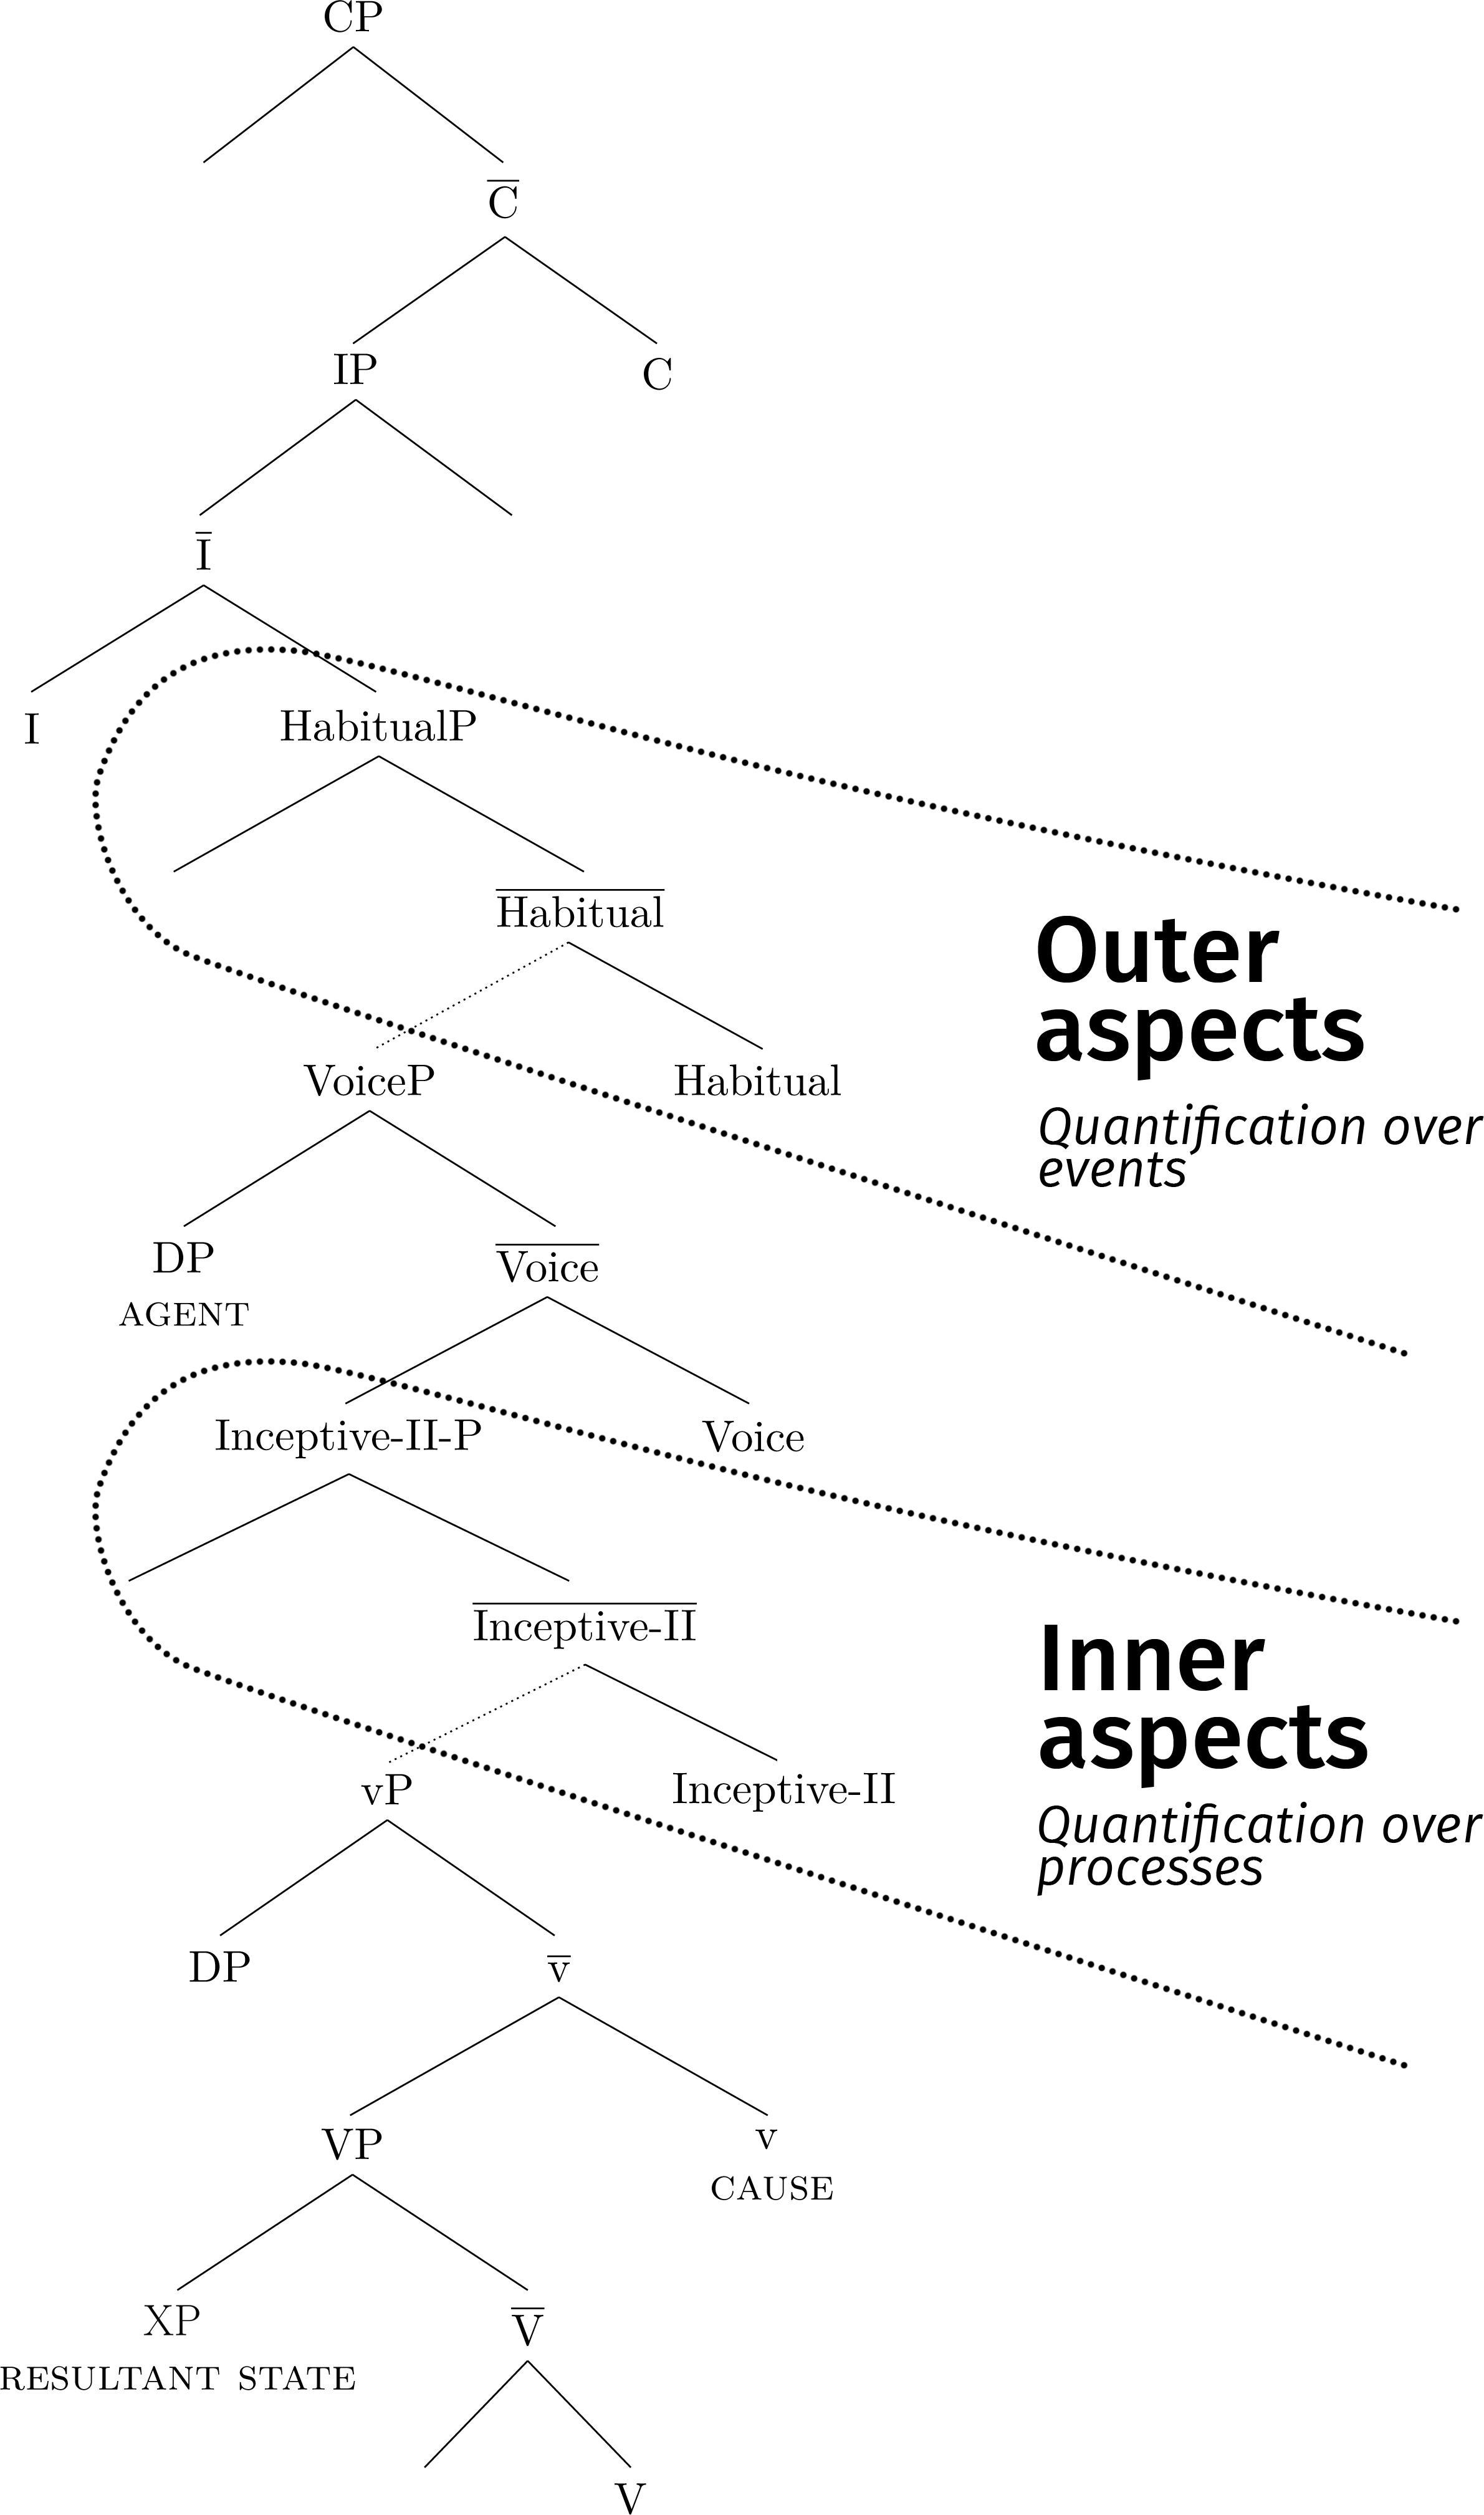
\includegraphics[width=\textwidth]{treesimplesw.jpg}
\begin{forest} for tree={calign=fixed angles,s sep=5ex}
[CP
 [\phantom{C}] [$\overline{\textrm{C}}$
  [IP 
   [$\overline{\textrm{I}}$,s sep=10ex
    [I] [HabitualP
     [\phantom{H}] [$\overline{\textrm{Habitual}}$,name=habitualbar
      [VoiceP, edge=dotted
       [DP\\\textsc{agent},align=center]
       [$\overline{\textrm{Voice}}$,s sep=5ex
        [Inceptive-II-P
        [\phantom{I}] [$\overline{\textrm{Inceptive-II}}$,name=inceptivebar,s sep=5ex
         [vP,edge=dotted
            [DP] [$\overline{\textrm{v}}$
              [VP
               [XP\\\textsc{resultant}\\\textsc{state}]
               [$\overline{\textrm{V}}$
                 [\phantom{V}] [V]
               ]
              ] [v\\\textsc{cause},align=center]
             ]
         ] [Inceptive-II,name=inceptive]
        ] 
       ] [Voice]
     ] 
   ] [Habitual,name=habitual] 
   ]
  ]
  ] [\phantom{I}]
  ] [C]
 ]   
]
\node[right=1cm of habitual,text width=3cm,align=left] (outer) {Outer aspects\\Quantification over events};
\path let \p1 = (inceptive), \p2 = (outer) in node at (\x2,\y1) [text width=3cm,align=left] (inner) {Inner aspects\\Quantification over processes};
\begin{scope}[on background layer]
\node at (habitualbar) [fill=gray!30, inner sep=0pt, ellipse, minimum width=2.5cm, minimum height=4.75cm, rotate=55,overlay] (outerarea)  {};
\node at (inceptivebar) [fill=gray!30, inner sep=0pt, ellipse, minimum width=2.5cm, minimum height=4.75cm, rotate=55,overlay] (innerarea)  {};
\end{scope}
\draw (outer.north west) -- (outerarea);
\draw (inner.north west) -- (innerarea);
\end{forest}
\end{figure}

\section{Habitual aspect (\textit{usually})}\label{habitualaspect}\is{habitual aspect|(}
\subsection{General overview}
According to \citet[28]{comrie1976aspect}, habitual aspect is used to ``describe a situation which is characteristic of an extended period of time, so extended in fact that the situation referred to is viewed not as an incidental property of the moment, but, precisely, as a characteristic feature of a whole period.'' Habitual aspect is set apart from the conceptually related frequentative aspect in that the latter describes the iteration of an event on a single occasion. 



\subsection{The situation in DGS}
Habitual aspect in DGS is expressed via the manual sign \textsc{usually} or the manual sign \textsc{typically} that are both located to the left of the VP as shown in (\ref{signusually}) and (\ref{singtypically}).

\begin{exe}
\ex\label{signusually}\begin{xlist} 
\ex[\phantom{*}] {{\textsc{paul usually apple buy}}
\glt `Paul usually buys an apple.' \label{ex:habituala}}
\ex[*] {{\textsc{paul apple buy usually}}
\glt `Paul usually buys an apple.' \label{ex:habitualb}}
\end{xlist}
\end{exe} 


\begin{exe}
\ex\label{singtypically}\begin{xlist} 
\ex[\phantom{*}] {{\textsc{paul typically apple buy}}
\glt `Paul usually buys an apple.' \label{ex:xhabituala}}
\ex[*] {{\textsc{paul apple buy typically}}
\glt `Paul usually buys an apple.' \label{ex:xhabitualb}}
\end{xlist}
\end{exe} 

\noindent No meaning difference between the two signs could be determined. When explicitly asked, the signers stated that they could use them interchangeably. This is in line with the fact that both signs, \textsc{usually} and \textsc{typically}, can be used with \is{animacy}animate and inanimate subjects (e.g., \textsc{cars typically/usually stink}). 

The data show that habitual aspect employs a manual-only strategy as was expected for a category below tense. Additionally, both instances of habitual aspect clearly concatenate from left to right. It has to be noted, however, that habitual aspect has been described as being expressed via \is{reduplication}reduplication of the verb stem in many sign languages including fast and smaller repetitions (e.g., \citealt{rathmann2005event} for American Sign Language). A similar claim has also been made for DGS. \citet[225]{signgram2017} cite the following example from DGS.

\begin{exe}
\ex \textsc{saturday index\textsubscript{1} shopping go+++} (fast \& small repetitions) 
\glt `I usually go shopping on Saturday.'\label{queretaldgs}
\end{exe}


\noindent \citet[148]{happ2014vork} also claim that habitual readings can be achieved by the \is{reduplication}reduplication of the verb sign, interrupted by short intonational breaks and give the following example (using their own glossing). 

\begin{exe}
\ex \textsc{interpreter fall-asleep}\textsubscript{habitual} 
\glt `The interpreter falls asleep habitually.'\label{habitualhappvorkoeper}

\end{exe}

\noindent From my own data, I can confirm that this is a possible strategy. Although there is no distinction between habitual aspect I and habitual aspect II, I claim that the \is{reduplication}reduplication strategy expresses a lower aspectual category located inside the VoiceP. Evidence that this is the case will be discussed in Section \ref{habitualtwo} where I show that the reduplication strategy cannot take scope over structurally higher modal verbs.

I will now briefly turn to the discussion of the combination of manually expressed habitual aspect and higher categories, namely habitual adverbs and deontic modals. On the assumption that deontic modals and habitual adverbs employ a left-to-right concatenation strategy in DGS, the order deontic $>$ habitual would be predicted. While this order is possible in DGS, as shown in (\ref{modalhabitualba}), the reverse order similarly is acceptable (\ref{modalhabitualc}) as are other ordering possibilities (\ref{modalhabitualbb}). Thus, testing this prediction did not yield the expected results.

\begin{exe}
\ex\label{modalhabitualb}\begin{xlist} 
\ex \textsc{paul must usually early at-home-be}
\glt `Usually, Paul must be at home early.'\label{modalhabitualba}
\ex \textsc{paul usually must early at-home-be}
\glt `Usually, Paul must be at home early.'\label{modalhabitualc}
\ex \textsc{paul usually early at-home-be must}
\glt `Usually, Paul must be at home early.'\label{modalhabitualbb}


\end{xlist}
\end{exe} 


\noindent This, again, seems to be a result of the relative freedom of deontic modals to occur in different positions and not a result of a violation of Cinque's hierarchy. This will become clear in the following sections which will show that the hierarchy generally predicts the right order of adverbs, but not the right order of adverbs and modal verbs. As discussed, this may have to do with the fact that modal verbs are heads and not phrases like the respective adverbs. That there are not two positions, but three for modal verbs when an adverb is present (as shown in (\ref{modalhabitualb})), is, in fact, predicted by Cinque. As already discussed in the introduction of this chapter (see the examples in (\ref{finiteauxcinque}) on page \pageref{finiteauxcinque}), auxiliary verbs can move to different head positions.

\is{habitual aspect|)}

\section{Delayed aspect (\textit{finally})}\is{delayed aspect|(}
\subsection{General overview}

Delayed aspect, first mentioned in \citet[105]{cinque1999adverbs} in a very short note, is tentatively assumed to be located between habitual aspect and predispositional aspect in \citet[93]{cinque2006restructuring}. His sources are a verbal suffix in Macushi (a Carib language) referring to ``procrastinated action'' according to \citet[119]{macushi}, a particle in the Austronesian language Ulithian referring to ``delayed action'' according to \citet[116]{sohn1980ulithian}, and the Italian verb \textit{finire} (\textit{per}). In the case of the Macushi suffix and the Ulithian particle, the respective authors translate the aspectual meaning with ``finally''. \citet[116]{sohn1980ulithian} define the meaning of this aspect as follows: ``It denotes the fact that the action had been previously anticipated or desired, but it is now finally undertaken.''

\subsection{The situation in DGS}
Delayed aspect is, again, expressed manually in DGS using a left-to-right concatenation strategy. The examples in (\ref{delayedaspectdgs}) illustrate this fact.

\begin{exe}
\ex Context: Already on Monday Paul said that he will take out the trash.\label{delayedaspectdgs}
\begin{xlist} 
\ex {\textcolor{white}{*}\textsc{today paul finally throw-out}}
\glt \textcolor{white}{*}`Today he finally took it out.' \label{ex:delayedaspectdgsa}
\ex {*\textsc{today paul throw-out finally}}
\glt\textcolor{white}{*} `Today he finally took it out.' \label{ex:delayedaspectdgsb}
\end{xlist}
\end{exe}  

\noindent Combining habitual and delayed aspect results in an order that would be expected from the left-to-right concatenation patterns of both aspects, namely \textsc{usually} $>$ \textsc{finally} and not the other way around. This is exemplified in (\ref{delayedaspectdgsusually}).

%\vspace{0.5cm}

\begin{exe}
\ex Context: Paul always claims that he takes out the trash on Monday.\label{delayedaspectdgsusually}
\begin{xlist} 
\ex {\textcolor{white}{*}\textsc{thursday usually finally throw-out}}
\glt \textcolor{white}{*}`It is usually a Thursday when he finally takes it out.' \label{ex:delayedaspectdgsusuallya}
\ex {*\textsc{thursday finally usually throw-out}}
\glt\textcolor{white}{*} `It is usually a Thursday when he finally takes it out.' \label{ex:delayedaspectdgsusuallyb}
\end{xlist}
\end{exe}  

%\subsection{The situation in DGS}
%Delayed aspect is, again, expressed manually in DGS using a left-to-right concatenation strategy. The examples in (\ref{delayedaspectdgs}) illustrate this fact.
%
%\begin{exe}
%\ex Context: Already on Monday Paul said that he will take out the trash. \label{delayedaspectdgs}\begin{xlist} 
%\ex {\textcolor{white}{*}\textsc{today paul finally throw-out}}
%\glt \textcolor{white}{*}`Today he finally took it out.' \label{ex:delayedaspectdgsa}
%\ex {*\textsc{today paul throw-out finally}}
%\glt\textcolor{white}{*} `Today he finally took it out.' \label{ex:delayedaspectdgsb}
%\end{xlist}
%\end{exe}  
%
%\noindent Combining habitual and delayed aspect results in an order that would be expected from the left-to-right concatenation patterns of both aspects, namely \textsc{usually} $>$ \textsc{finally} and not the other way around. This is exemplified in (\ref{delayedaspectdgsusually}).
%
%\vspace{0.5cm}
%
%\begin{exe}
%\ex Context: Paul always claims that he takes out the garbage on Monday. \label{delayedaspectdgsusually}\begin{xlist} 
%\ex {\textcolor{white}{*}\textsc{thursday usually finally throw-out}}
%\glt \textcolor{white}{*}`It is usually a Thursday when he finally takes it out.' \label{ex:delayedaspectdgsusuallya}
%\ex {*\textsc{thursday finally usually throw-out}}
%\glt\textcolor{white}{*} `It is usually a Thursday when he finally takes it out.' \label{ex:delayedaspectdgsusuallyb}
%\end{xlist}
%\end{exe}  
%
%\noindent In contrast to the combination of adverbs with modal verbs in the previous section, the order predicted by Cinque's scopal hierarchy results in the expected order in the case of combining adverbs. Thus, combining adverb phrases hosted in specifiers results in the right pattern, but not combining a phrase and a head. This leads to the prediction that the combination of modals verbs (i.e., combining a head with a head) should also lead to the patterns predicted by the hierarchy. This prediction will be tested in Section \ref{rootmodality}.
%
%To conclude, delayed aspect is expressed manually in DGS. The manual sign \textsc{finally} employs a left-to-right concatenation strategy. Combining a delayed aspectual adverb with a habitual adverb resulted in the order predicted by the suggestion that habitual aspect scopes higher than delayed aspect.  

\is{delayed aspect|)}

\section{Predispositional aspect (\textit{tendentially})}\is{predispositional aspect|(}
\subsection{General overview}
Predispositional aspect is not defined by \citet{cinque1999adverbs, cinque2006restructuring}, but simply paraphrased with either \textit{tendentially} or \textit{tend to}. 

\subsection{The situation in DGS}
I have found no evidence of the expression of predispositional aspect in DGS. A manual sign with the meaning of \textit{tendentially} does not seem to exist. In most instances of predispositional aspect in my data, signers used the adverbs \textsc{typically} or \textsc{usually} that were described in Section \ref{habitualaspect}, as shown in (\ref{fluctuateexample}). In such cases, the movement of the verb sign is not modified. 

\begin{exe}
\ex \textsc{prices typically fluctuate}
\glt `The prices tendentially fluctuate./The prices typically fluctuate.' \label{fluctuateexample}
\end{exe}

\noindent It has to be noted, however, that the expression of predispositional aspect has been described as being expressed by changing the movement path of the verb sign for some sign languages. Most notably, \citet[249]{klima1979signs} claim that a large, circular \is{reduplication}reduplication of the verb sign indicates predispositional aspect which they paraphrase with \textit{tend to} in \is{American Sign Language}American Sign Language (see also \citealt{rathmann2005event}). However, this modulation is only possible for a very restricted set of signs referring to incidental or temporary states (e.g., \textsc{angry}, \textsc{sick}, or \textsc{dirty}). I have not made a similar observation for DGS, although I do not exclude the possibility that this is possible for a restricted class of verbs.  
\is{predispositional aspect|)}

\section{Repetitive aspect I (\textit{again})}\label{repetitiveonesection}\is{repetitive aspect I|(}
\subsection{General overview}

While habitual aspect refers to the iteration of an event over a longer period of time, repetitive aspect I refers to the iteration of an event on a single occasion. In contrast to frequentative aspect I (see the next section), repetitive aspect I refers to a single iteration. An instance of repetitive aspect is the adverb \textit{again}. As discussed in Section \ref{generalaspect}, repetitive aspect I quantifies over events while repetitive aspect II quantifies over processes. Repetitive aspect II will be discussed in Section \ref{repetitivetwo} (see page \pageref{repetitivetwo}). 

\subsection{The situation in DGS}
Repetitive aspect I is expressed manually in DGS. The sign \textsc{again} is concatenated using a left-to-right strategy, as shown in (\ref{ex:repetitiveone}). Using \textsc{again} clause-finally results in an odd structure if there is no pause before the sign or some focus marking (\ref{ex:repetitiveonb}).

\begin{exe}
\ex\begin{xlist} 
\ex {\textcolor{white}{?}\textsc{paul again door knock}}
\glt \textcolor{white}{?}`Paul knocks on the door again.' \label{ex:repetitiveone}
\ex {?\textsc{paul door knock again}}
\glt \textcolor{white}{?}`Paul knocks on the door again.' \label{ex:repetitiveonb}
\end{xlist}
\end{exe}  

\noindent Taken together, repetitive aspect I employs a manual-only strategy and is concatenated from left-to-right. 

\is{repetitive aspect I|)}

\section{Frequentative aspect I (\textit{often})}\label{frequentative}\is{frequentative aspect I|(}
\subsection{General overview}
As with repetitive aspect I and II, frequentative aspect I and II differ in their scope. Just as with repetitive aspect I, frequentative aspect I quantifies over an event over a longer period of time and just as with repetitive aspect II, frequentative aspect II quantifies over an event on a single occasion (or a process). For \citet{cinque1999adverbs}, instances of frequentative aspect are \textit{often} and \textit{seldom}. Taking the example of \textit{often} and a knocking event, frequentative aspect I refers to several knocking events on different occasions (e.g., a scenario where Paul knocks on my door every day) and frequentative II refers to several knocking events on one occasion (e.g., I'm sleeping and Paul has been standing outside the door for three minutes and repeats his knocking often), as discussed in Section \ref{generalaspect}.

\subsection{The situation in DGS}
Frequentative aspect I is only expressed manually in DGS. As with the other aspects discussed so far, a left-to-right concatenation strategy is more frequently employed than the reverse pattern. This is illustrated in (\ref{ex:frequentativea}). For some signers, clause-final \textsc{often}, as in (\ref{ex:frequentativeb}), is acceptable, while for others it was clearly ill-formed (therefore I marked it with a question mark). With \textsc{seldom}, the intuitions seemed to be sharper, as it only was allowed pre-verbally as in (\ref{ex:frequentativecz}) and not post-verbally as in (\ref{ex:frequentativedz}).


\begin{exe}
\ex\begin{xlist} 
\ex[] {{\textsc{anna often apple buy}}
\glt `Anna often buys an apple.' \label{ex:frequentativea}}
\ex[?*] {{\textsc{anna apple buy often}}
\glt `Anna often buys an apple.' \label{ex:frequentativeb}}
\end{xlist}
\end{exe} 

\begin{exe}
\ex\label{referbacktome}\begin{xlist} 
\ex[] {{\textsc{jun door seldom knock}}
\glt `Jun seldom knocks on the door.' \label{ex:frequentativecz}}
\ex[*] {{\textsc{jun door knock seldom}}
\glt `Jun seldom knocks on the door.' \label{ex:frequentativedz}}
\end{xlist}
\end{exe}   

%\begin{exe}
%\ex\begin{xlist} 

%%\glll {}
%%{} {\hspace{343pt}}  \\
%\ex {\textcolor{white}{?*}\textsc{anna often apple buy}}
%\glt \textcolor{white}{?*}`Anna often buys an apple.' %\label{ex:frequentativea}
%\ex {?*\textsc{anna apple buy often}}
%\glt \textcolor{white}{?*}`Anna often buys an apple.' %\label{ex:frequentativeb}
%\end{xlist}
%\end{exe} 

%\begin{exe}
%\ex\label{referbacktome}\begin{xlist} 
%\ex {\textcolor{white}{*}\textsc{jun door seldom knock}}
%\glt \textcolor{white}{*}`Jun seldom knocks on the door.' %\label{ex:frequentativecz}
%\ex {*\textsc{jun door knock seldom}}
%\glt \textcolor{white}{*}`Jun seldom knocks on the door.' %\label{ex:frequentativedz}
%\end{xlist}
%\end{exe}   

\noindent Note that \textsc{often} in (\ref{ex:frequentativea}) precedes the object and \textsc{seldom} in (\ref{ex:frequentativecz}) appears to the right of the object. This is an artifact of object movement (while there are no definite and indefinite articles in DGS, the natural landing site for definite objects is preceding manual IP-internal adverbs and indefinite objects follow manual adverbs). 

Combining habitual and frequentative aspect only allows for the orders \textsc{usually often} and \textsc{typically often}. As expected from the left-to-right concatenation strategy, the inverse orders *\textsc{often usually} and *\textsc{often typically} are disallowed. This is illustrated in (\ref{combininghabitualandfrequentative}). 




\begin{exe}
\ex\label{combininghabitualandfrequentative}\begin{xlist} 
\ex[] {{\textsc{paul usually often at-home}}
\glt `Usually, Paul is often at home.' \label{ex:frequentativec}}
\ex[*] {{\textsc{paul often usually at-home}}
\glt `Usually, Paul is often at home.'  \label{ex:frequentatived}}
\end{xlist}
\end{exe} 

\noindent Similarly, a combination of repetitive I and frequentative I leads to the order \textsc{again often} and not the other way around: 

\begin{exe}
\ex Context: In the past Paul often brought beer. \label{xcombininghabitualandfrequentative}\begin{xlist} 
\ex[] {{\textsc{now paul again often beer buy}}
\glt `Now Paul again often buys beer.' \label{ex:xfrequentativec}}
\ex[*] {{\textsc{now paul often again beer buy}}
\glt `Now Paul again often buys beer.'  \label{ex:xfrequentatived}}
\end{xlist}
\end{exe} 

\noindent The examples show, again, that the combination of manual adverbs results in the order predicted by the general scope-taking hierarchy. Thus, frequentative aspect I is expressed manually using a left-to-right concatenation strategy -- just like the other aspectual categories discussed so far.

\is{frequentative aspect I|)}



\section{Volition/Bouletic modality (\textit{intentionally}/\textit{want})}\label{volition}\is{volition|(}\is{bouletic modality|see{volition}}
\subsection{General overview}
Volition, sometimes called bouletic modality, refers to the wishes, desires, and plans of the subject. In English, volition can be expressed by adverbs like \textit{intentionally} or by verbs like \textit{want}.

\subsection{The situation in DGS}


While manual modal verbs generally appear to the left or to the right of the VP, it has been noted that the volitional markers \textsc{wish} and \textsc{plan} systematically appear to the left of the verb in DGS (\citealt[326]{happ2014vork}; \citealt[20]{bross2017scope}). A pre-verbal position was indeed the most favored position for all of my consultants. Again, volition is expressed via a manual-only strategy and no non-manual markers are involved. 

Although the post-verbal position is not the preferred slot, volitional modals are allowed in this position. Additionally, as with the other manual modals discussed so far, volitional modals can receive stress in both positions. The two (unstressed) options are shown in (\ref{volitionalmodalsdgs}).

\begin{exe}
\ex\label{volitionalmodalsdgs}\begin{xlist}
\ex \textsc{paul wish beer drink} 
\ex \textsc{paul beer drink wish} 
\end{xlist}
\end{exe}

\noindent Instead of the modal verb signs \textsc{wish} and \textsc{plan} the adverb sign \textsc{absolutely} can be used and is actually preferred by some signers. In this case, \textsc{absolutely} clearly employs a left-to-right-concatenation strategy as shown in (\ref{ex:absolutelya}) and (\ref{ex:absolutelyb}).\footnote{ Note that I ignore cases in which a clause-final adverb can occur given that it is preceded by an intonational break. \citet[283]{happ2014vork} give one example with a clause-final use of \textsc{absolutely}, but also transcribe a pause in this case. } 

\begin{exe}
\ex\begin{xlist} 
\ex {\textcolor{white}{*}\textsc{paul absolutely apple buy}}
\glt \textcolor{white}{*}`Paul wants to buy an apple' \label{ex:absolutelya}
\ex {*\textsc{paul apple buy absolutely}}
\glt \textcolor{white}{*}`Paul wants to buy an apple.'  \label{ex:absolutelyb}
\end{xlist}
\end{exe} 

\noindent The same is true for the adjectival sign \textsc{intentionally}:

\begin{exe}
\ex\begin{xlist} 
\ex {\textcolor{white}{*}\textsc{paul game intentionally lose}}
\glt \textcolor{white}{*}`Paul loses the game intentionally.' \label{ex:intentionallya}
\ex {*\textsc{paul game lose intentionally}}
\glt \textcolor{white}{*}`Paul loses the game intentionally.'  \label{ex:intentionallyb}
\end{xlist}
\end{exe} 

\noindent As already noted for the examples in (\ref{referbacktome}) (see page \pageref{referbacktome}), the question whether an adverb precedes the object (as in (\ref{ex:absolutelya})) or follows it (as in (\ref{ex:absolutelyb})) is an artifact of object shift: Definite objects precede the adverb and indefinite objects follow the adverb. 

When asked to sign a sentence like \textit{Paul unintentionally bought the book} some signers used the sign \textsc{wrong} -- possibly as an adverb and not as an adjective modifying a noun -- for \textit{unintentionally}. The sign \textsc{wrong} behaves in the same way, i.e., it only occurs pre-verbally:

\begin{exe}
\ex\begin{xlist} 
\ex {\textcolor{white}{*}\textsc{paul book wrong buy}}
\glt \textcolor{white}{*}`Paul bought the book unintentionally.' \label{ex:xintentionallya}
\ex {*\textsc{paul book buy wrong}}
\glt \textcolor{white}{*}`Paul bought the book unintentionally.'  \label{ex:xintentionallyb}
\end{xlist}
\end{exe} 

\noindent These findings, again, illustrate that modal verbs can be positioned more freely than adverbs in DGS. The combination of bouletic modal verbs and root modals will be discussed in Section \ref{rootmodality}. In this section, it will become clear that modal verbs amongst themselves behave in the predicted way (i.e., volition scopes higher than root modality). 

Combining volitional adverbs with higher adverbs, such as \textsc{often} as an instance of frequentative aspect I, gives the expected results as \textsc{often} has to precede \textsc{intentionally} as shown in (\ref{oftenintentionally}). 

\begin{exe}
\ex\label{oftenintentionally}\begin{xlist} 
\ex {\textcolor{white}{*}\textsc{paul pam maria often intentionally insult}}
\glt \textcolor{white}{*}`Paul often insults Maria intentionally.' \label{ex:oftenintentionallya}
\ex {*\textsc{paul pam maria intentionally often insult}}
\glt \textcolor{white}{*}`Paul often insults Maria intentionally.'  \label{ex:oftenintentionallyb}
\end{xlist}
\end{exe} 

\noindent The same is true with other higher adverbs, such as the habitual adverbs \textsc{usually} or \textsc{typically} that also have to precede \textsc{intentionally} as shown in (\ref{usuallyintentionally}).

\begin{exe}
\ex\label{usuallyintentionally}\begin{xlist} 
\ex {\textcolor{white}{*}\textsc{paul game typically intentionally lose}}
\glt \textcolor{white}{*}`Paul usually loses the game intentionally.' \label{ex:usuallyintentionallya}
\ex {*\textsc{paul game intentionally typically lose}}
\glt \textcolor{white}{*}`Paul usually loses the game intentionally.'  \label{ex:usuallyintentionallyb}
\end{xlist}
\end{exe} 

\noindent Taken together, volition is expressed with a manual-only strategy by concatenating manual adverbs from left to right. For volitional modal verbs, more positional freedom was observed, although they are preferably signed pre-verbally.

\is{volition|)}

\section{Celerative aspect I (\textit{quickly})}\label{celerativeone}\is{celerative aspect I|(}
\subsection{General overview}
As with the other aspects that are referred to by the numbers I and II, celerative aspect can either quantify over an event (celerative aspect I) or a process (celerative aspect II) (see also \citealt{travis1988syntax, tennyl2000core, ernst2002syntax}). An instance of celerative aspect is the adverb \textit{quickly} (\citealt[292]{travis1988syntax}; \citealt[93]{cinque1999adverbs}). When \textit{quickly} quantifies over an event, it can be paraphrased with \textit{being quick to} (celerative I) and when it quantifies over a process it can be paraphrased with \textit{in a quick way}. The two readings are, again, tied to different syntactic positions, as illustrated for English in (\ref{quicklyrasing}).

\begin{exe}
\ex\label{quicklyrasing}\begin{xlist}
\ex Paul quickly raised his hand. \hfill{\textit{Celerative I (\textit{being quick to})}} \label{quicklyrasinga}
\ex Paul raised his hand quickly.\hfill{\textit{Celerative II (\textit{in a quick way})}} \label{quicklyrasingb}
\end{xlist}
\end{exe}  

\noindent In the case of celerative I in (\ref{quicklyrasinga}), Paul's raising of the hand can actually be very slow. The reading that is aimed at here is that his raising of the hand is quick with reference to another event. Assume the teacher is asking a very tough question and all the students are thinking hard to find an answer. However, Paul is the first one to find this answer, so in relation to the other students (or in relation to the event of the question being asked), he is quick to raise his hand. In (\ref{quicklyrasingb}), this is different. Now it is the motion of Paul's hand itself that is quick. Celerative aspect II will be discussed in Section \ref{celerativetwo} (see page \pageref{celerativetwo}).

\subsection{The situation in DGS}

Celerative aspect I is expressed manually via the sign \textsc{fast}. As shown in (\ref{ex:xafrequentativec}) it precedes the VP. The example in (\ref{ex:xafrequentatived}) shows that the same sentence becomes less acceptable when \textsc{fast} follows the VP. 

\begin{exe}
\ex\begin{xlist} 
\ex {\textcolor{white}{?}\textsc{paul fast raises-his-hand}}
\glt \textcolor{white}{?}`Paul raises his hand quickly.' \label{ex:xafrequentativec}
\ex {?\textsc{paul raises-his-hand fast}}
\glt \textcolor{white}{?}`Paul raises his hand quickly.'  \label{ex:xafrequentatived}
\end{xlist}
\end{exe} 

\noindent To conclude, celerative aspect I is expressed by a manual-only strategy. However, it can be combined with several non-manual markers to express the signer's evaluation of the event. 
\is{celerative aspect I|(}

%\vspace{-0.5cm}
\section{Anterior tense (\textit{already})}\is{anterior tense|(}
\subsection{General overview}
nterior tense, identified by \citet[94]{cinque1999adverbs} with the adverb \textit{already}, refers to temporal priority: ``The adverb \textit{already} forces a priority reading for the event expressed in the sentence in which it is found'' \citep[547]{hornstein1977towards}. This means that the proposition expressed in a sentence will be interpreted as being located before the reference time. To illustrate this, \citet[94]{cinque1999adverbs} uses the two example sentences in (\ref{alreadyexamplesone}) and (\ref{alreadyexamplesoneb}).

\begin{exe}
\ex\label{alreadyexamplesone}\begin{xlist} 
\ex Haven't we met? \label{alreadyexampleaa}
\ex Last Christmas, hadn't they met? \label{alreadyexampleab}
\end{xlist}
\end{exe} 

\begin{exe}
\ex\label{alreadyexamplesoneb}\begin{xlist}  
\ex Haven't we already met? \label{alreadyexamplea}
\ex Last Christmas, hadn't they already met? \label{alreadyexampleb}
\end{xlist}
\end{exe} 

\noindent The examples show that the meaning difference between the sentences without (\ref{alreadyexamplesone}) and with \textit{already} (\ref{alreadyexamplesoneb}) is only minimal. The difference between (\ref{alreadyexampleaa}) and (\ref{alreadyexamplea}) is that in the latter we find the additional presupposition that the encounter is located before the reference time, which in this example is the speech time. The difference between (\ref{alreadyexampleab}) and (\ref{alreadyexampleb}) is that in the latter we find the additional presupposition that the encounter is located before the reference time, which in this example is last Christmas.

\subsection{The situation in DGS}
The translational equivalent of \textit{already} is expressed manually with the sign \textsc{already} in DGS.\footnote{ Note that the sign \textsc{already} is different from what is usually labeled \textsc{perf} (for perfect aspect), a sign which is accompanied by the mouthing \textit{gewesen} `been' (see, for example, \citealt[292]{happ2014vork}). It is, however, similar to the sign \textsc{finish} that was also described as a perfect marker. However, \textsc{finish} and \textsc{already} are accompanied by different mouthings.} This sign, again, appears to the left of the VP, as shown in the examples in (\ref{papasssssalready}) from \citet[155]{papaspyrou2008grammatik}.

\begin{exe}
\ex\label{papasssssalready}\begin{xlist} 
\ex \textsc{boss already gone} 
\glt `The boss is already gone.' \label{alreadygonepapaa}
%\ex $\frac{\hfill\textrm{wh}}{\textrm{\textsc{poss}\textsubscript{2} \textsc{daughter already school}\textsubscript{3a} \textsc{go}\textsubscript{3a}}}$
\ex \textsc{poss}\textsubscript{2} \textsc{daughter already school}\textsubscript{3a} \textsc{go}\textsubscript{3a}
\glt `Your daughter already went to school.' \label{alreadygonepapab}
\end{xlist}
\end{exe} 

\noindent That the natural position of \textsc{already} is pre-verbal is also confirmed by my own data. Combining celerative aspect I and anterior tense leads to the predicted results, namely that the adverb \textsc{already} has to precede \textsc{quickly}, as shown in (\ref{quicklyalready}).

\begin{exe}
\ex\label{quicklyalready}\begin{xlist} 
\ex \textcolor{white}{*}\textsc{paul already quickly raise-hand} \label{quicklyalreadya}
\glt \textcolor{white}{*}`Paul had already quickly raised his hand.'
\ex *\textsc{paul quickly already raise-hand}
\glt \textcolor{white}{*}`Paul had already quickly raised his hand.'\label{quicklyalreadyb}
\end{xlist}
\end{exe} 

\noindent Additionally, there is a sign \textsc{not-yet} that behaves in exactly the same way as \textsc{already}, as shown in (\ref{ex:notyetexamples}).

\begin{exe}
\ex\label{ex:notyetexamples}\begin{xlist} 
\ex \textcolor{white}{*}\slg{paul} \slg[hs]{not-yet} \slg{apple++ buy}
%{} {\hspace{72pt}hs} {}    \\
%{\textcolor{white}{*}\textsc{paul}} {$\overline{\textrm{\textsc{not-yet}}}$}  {\textsc{apple++ buy}}      
\glt \textcolor{white}{*}`Paul hasn't bought apples yet.' \label{ex:notyetexamplesa}
\ex *\slg{paul} \slg{apple++ buy} \slg[hs]{not-yet}
%\ex
%{} {} {\hspace{156pt}hs}    \\
%{*\textsc{paul}}  {\textsc{apple++ buy}} {$\overline{\textrm{\textsc{not-yet}}}$}     
\glt \textcolor{white}{*}`Paul hasn't bought apples yet.' \label{ex:notyetexamplesb}

\end{xlist}
\end{exe}

\noindent Thus, anterior tense is, again, expressed manually-only, employing a left-to-right concatenation strategy, and combines with other manual adverbs as predicted by the Cinquean hierarchy. It has to be noted, however, that a clause-final use of \textsc{not-yet} was reported in the literature \citep[185]{papaspyrou2008grammatik}. Future research should check the option if this is due to dialectal variation.

It should be stressed that \textit{already}, as well as other phrasal adverbials that will be discussed in the following (\textit{no longer} and \textit{still}), also have non-temporal uses (e.g., \citealt{konig1977temporal, lobner1989germanschon, van1998phasal}) that should be investigated separately in future studies.

\is{anterior tense|)}

\section{Terminative aspect (\textit{no longer})}\is{terminative aspect|(}
\subsection{General overview}
Terminative aspect, also called cessative aspect (e.g., \citealt{binnick1991time}), marks the termination of an event, bound or unbound, at an arbitrary point \citep[70]{cinque2006restructuring}, e.g., \textit{to stop smoking}. \citeauthor{cinque1999adverbs}'s (\citeyear{cinque1999adverbs}: 94--95) example of terminative aspect is \textit{no longer}. 

\subsection{The situation in DGS}
The translational equivalent of \textit{no longer} in DGS is the sign \textsc{no-longer}. \citet[377]{happ2014vork} claim that it has to occur clause-finally and that it cannot precede the verb. Additionally, in their transcription they indicate that it is signed after a short pause. See the examples in (\ref{nolongerhappvorkoeper}), from \citet[377]{happ2014vork}. 


\begin{exe}
\ex\label{nolongerhappvorkoeper}\begin{xlist} 
\ex[\textcolor{white}{*}]{\textsc{osolemirnix}\textsubscript{3a} \textsc{aszurnix}\textsubscript{3b} \textsc{idx}\textsubscript{3a-3b(dual)}, \textsc{fight no-longer}
\glt `Osolemirnix and Aszurnix do not fight any more.' \label{nolongerhappvorkoepera}}
\ex[*]{\textsc{osolemirnix}\textsubscript{3a} \textsc{aszurnix}\textsubscript{3b} \textsc{idx}\textsubscript{3a-3b(dual)} \textsc{no-longer fight}
\glt `Osolemirnix and Aszurnix do not fight any more.' \label{nolongerhappvorkoeperb}}
\end{xlist}

\end{exe} 


\noindent Despite this, my consultants produced \textsc{no-longer} both preceding and following the verb. The preferred position was subject to inter-signer variation. As \textsc{no-longer} has an inherently negative meaning it is accompanied by a head shake. This head shake, however, does not spread over the verb, as shown in (\ref{ex:nolongermydata}).

%
\begin{exe}
\ex\label{ex:nolongermydata}\begin{xlist} 
\ex \slg{paul} \slg[hs]{no-longer} \slg{dance}
%{} {\hspace{80pt}hs} {}   \\
%{\textsc{paul}} {$\overline{\textrm{\textsc{no-longer}}}$} {\textsc{dance}}      
\glt `Paul does not dance any more.' \label{ex:nolongermydataa}
\ex \slg{paul dance} \slg[hs]{no-longer}
%\ex
%{} {} {\hspace{120.5pt}hs}   \\
%{\textsc{paul}} {\textsc{dance}}  {$\overline{\textrm{\textsc{no-longer}}}$}      
\glt `Paul does not dance any more.' \label{ex:nolongermydatab}
\end{xlist}
\end{exe}

\noindent As indicated by the glosses in (\ref{ex:nolongermydata}) my consultants did not make any significant intonational breaks before or after signing \textit{no-longer}. It still remains unclear whether there are any meaning differences between the position of the adverb. My consultants allowed both orders in contexts where the termination of the event referred to a single event (e.g. \textit{Paul danced for five hours}) or to a longer-lasting behavior (e.\,.g., \textit{Paul was a dancer for ten years}). 

For some signers, the judgements were clearer for the signs \textsc{interrupt} shown in (\ref{ex:interrupt}) and \textsc{stop} shown in (\ref{ex:stopped}) that can both be used to express the termination of an event at an arbitrary point. 

\begin{exe}
\ex\label{ex:interrupt}\begin{xlist} 
\ex
{\textcolor{white}{?}\textsc{paul interrupt eat}}      
\glt \textcolor{white}{?}`Paul stopped eating.' \label{ex:interrupta}
\ex
{?\textsc{paul eat interrupt}}       
\glt \textcolor{white}{?}`Paul stopped eating.' \label{ex:interruptb}
\end{xlist}
\end{exe}

\begin{exe}
\ex\label{ex:stopped}\begin{xlist} 
\ex
{\textcolor{white}{?}\textsc{paul stop eat}}      
\glt \textcolor{white}{*}`Paul stopped eating.' \label{ex:stoppeda}
\ex
{?\textsc{paul eat stop}}       
\glt \textcolor{white}{?}`Paul stopped eating.' \label{ex:stoppedb}
\end{xlist}
\end{exe}

\noindent However, there was again some inter-signer variation as some signers only allowed for a pre-verbal position and others accepted both orders. I will leave this point open for further research. 

Note that for \is{American Sign Language}American Sign Language it has been observed that the termination of an event can be expressed by a hold morpheme \citep{brentari1998prosodic, wilbur2000when, rathmann2005event} that ``takes the phonological form of freezing the final configuration of the sign'' \citep[43]{rathmann2005event}. I did not find a comparable morpheme and the majority of the signers I consulted did not accept constructions with signs involving interrupted movements. See also the discussion of conative aspect in Section \ref{conative} under which the hold morpheme was also subsumed.

Taken together, terminative aspect is signed manually in DGS, but the question of whether it concatenates from left to right or from right to left could not be resolved completely. 


\is{terminative aspect|)}

\section{Continuative aspect I (\textit{still})}\label{continuativeone}\is{continuative aspect|(}
\subsection{General overview}
Although continuative aspect and terminative aspect are very similar, \citet[95]{cinque1999adverbs} argues that they are distinct. He treats the adverb \textit{still} as an instance of continuative aspect. \citet{cinque1999adverbs} takes this to be the positive counterpart of \textit{no longer} (but nevertheless argues that continuative and terminative are two distinct classes). Later, in \citet{cinque2006restructuring}, he distinguishes continuative aspect I from a lower continuative II  that is located below Voice. While continuative aspect I refers to the continuation of an event, continuative aspect II relates to a process. Thus, continuative I is acceptable in contexts that refer to a larger time-frame (e.g., \textit{Paul has been a professional dancer for the last five years and he still dances}) while continuative II refers to an action that is still in progress (e.g., \textit{Paul has been dancing for two hours and he is still dancing}). I will discuss continuative aspect II in Section \ref{continuativetwo} (see page \pageref{continuativetwo}).

\subsection{The situation in DGS}
The adverb \textit{still} is expressed manually in DGS. The manual adverb \textsc{still} employs a left-to-right concatenation strategy as shown in (\ref{ex:whatisthislabel}).

\begin{exe}
\ex\label{ex:whatisthislabel}\begin{xlist} 
\ex[\textcolor{white}{*}] {{\textsc{kassandra still dance}} 
\glt `Kassandra still dances.'}
\ex[*] {{\textsc{kassandra dance still}}
\glt `Kassandra still dances.'}
\end{xlist}
\end{exe}




\noindent In conclusion, the continuative aspect markers discussed in this section behave in the predicted way as they are marked manually-only and concatenate from left to right.

A final note on continuative aspect (and probably continuative aspect I) concerns the sign \textsc{through} that is mentioned as a continuative marker in DGS in \citet[259]{rathmann2005event} and is glossed \textsc{durch} there. I did not observe this sign in my data -- at least not as a marker for continuative aspect. More research in this area is needed. However, I will briefly come back to \textsc{through} in the side-note on page \pageref{exkursfertigdurch}.

\is{continuative aspect|(}



\section{Perfect/Imperfect aspect(?) (\textit{always})}\is{perfect aspect|(}\is{imperfect aspect|see{perfect aspect}}
\subsection{General overview}
The projection following continuative aspect I is (somehow confusingly) labeled `perfect/imperfect aspect(?)' by \citet[96]{cinque1999adverbs}. He discusses this category by looking at the distribution of the continuative adverb \textit{ancora} `still' with regard to \textit{sempre} `always'. As illustrated in (\ref{ex:perfecta}) and (\ref{ex:perfectbb}), \textit{sempre} has to follow \textit{ancora} when both occur in one clause. However, he also remarks that ``[w]hether it [\textit{sempre}] should be related to Asp\textsubscript{perfect/imperfect} remains unclear'' \citep[96]{cinque1999adverbs}. 

\begin{exe}
\ex Italian \citep[96]{cinque1999adverbs}\begin{xlist} 
\ex {\textcolor{white}{*?}{Gianni vince \textit{ancora} \textit{sempre} tutte le partite.} 
\glt \textcolor{white}{*?}`Gianni still always wins all the games.' \label{ex:perfecta}}
\ex *?{{Gianni vince \textit{sempre} \textit{ancora} tutte le partite.}
\glt \textcolor{white}{*?}`Gianni still always wins all the games.' \label{ex:perfectbb}}
\end{xlist}
\end{exe} 

\noindent Besides the possibility that \textit{sempre} belongs to an imperfect aspectual category, he also discusses the possibility that it relates to continuous aspect. 

\subsection{The situation in DGS}
Whatever the label of this category may be, \textit{always} in DGS is realized with the manual sign \textsc{always}. This manual adverb naturally precedes the VP as illustrated in (\ref{ex:perfect}). Again, a post-verbal position does not result in an acceptable structure. However, some signers produced \textsc{always} post-verbally, but only after a short intonational break and with the adverb in focus.  

\begin{exe}
\ex\label{alwaysbeerbuy}\begin{xlist}
\ex {\textcolor{white}{?}\textsc{paul always beer buy}} 
\glt \textcolor{white}{?}`Paul always buys beer.' \label{ex:perfect}
\ex {?\textsc{paul beer buy always}} 
\glt \textcolor{white}{?}`Paul always buys beer.' \label{ex:perfectb}
\end{xlist}
\end{exe} 

\noindent I take this as evidence that the natural position of \textsc{always} is before the VP and conclude that what is called perfect aspect is expressed using a left-to-right concatenation strategy. Note that several different versions of the sign \textsc{always} exist and all behave in the same way.




\is{perfect aspect|(}


\section{Retrospective aspect (\textit{just})}\label{justjust}\is{retrospective aspect|(}
\subsection{General overview}
Retrospective aspect expresses ``the fact that the event has taken place a short while before some reference time'' \citep[96]{cinque1999adverbs}. \citet{cinque1999adverbs} takes \textit{just} as an instance of retrospective aspect. 

\subsection{The situation in DGS}
This adverb is expressed manually in DGS. The sign \textsc{just} has to appear pre-verbally, as shown in (\ref{retroretrodgs}).


\begin{exe}

\ex\label{retroretrodgs}\begin{xlist} 
\ex \textcolor{white}{*}\slg{paul} \slg[$==$]{just} \slg{bath}
%
%\ex {} {\hspace{48pt}$= =$} {}  \\ 
%{\textcolor{white}{*}\textsc{paul}} {$\overline{\textrm{\textsc{just}}}$} {\textsc{bath}} 
\glt \textcolor{white}{*}`Paul just took a bath.' \label{ex:retrospectivea}
\ex *\slg{paul} \slg{bath} \slg[$==$]{just}
%
%\ex {} {\hspace{79pt}$= =$} \\
%{*\textsc{paul just}} {$\overline{\textrm{\textsc{just}}}$}
\glt \textcolor{white}{*}`Paul just took a bath.' \label{ex:retrospectiveb}
\end{xlist}
\end{exe} 


\noindent Note that the sign \textsc{just} is accompanied by sucked-in cheeks \citep[40]{herrmann2013modal}, by pursed/tensed lips, or by pursed/tensed lips with an additional tongue protrusion. In the examples above, I glossed tensed lips by using the symbol `$= =$'. The meaning of this non-manual marking is to evaluate that the time span talked about is small (in the sense of scalarity discussed in Section \ref{scalarity}) and is thus an expression of a higher category. Similar observations can be made with other signs expressing concepts that have an evaluative component (e.g., \textsc{thin} is accompanied by similar non-manuals). Note that the non-manual modification of \textsc{just} is obligatory while the strength of the evaluation (i.e., the degree to which the lips are pursed or the tongue is protruded) is variable. This is shown in Figure \ref{fig:just}. The figure shows three instances of the sign \textsc{just} with increasing intensity of the evaluation. 

I take the non-manuals accompanying \textsc{just} as an instantiation of the idea that ``some `lexical' items may$[$\dots$]$ be decomposed into a lexical core surrounded by functional material'' (\citealt[424]{shlonsky2010cartographic}; see also \citealt{kayne2005some, kayne2007several}). Thus, the manual sign expresses ``the fact that the event has taken place a short while before some reference time'' \citep[96]{cinque1999adverbs}, while the non-manuals indicate the degree to which the signer evaluates how small the time interval is. It is worth noting that there are many signs which are specified for lexical non-manuals, similar to \textsc{just}. Concerning the bodily-mapping hypothesis, these signs will need more attention in the future. For a discussion of lexical non-manuals in DGS see \citet{pendzich2017lexicalnmms}.

\begin{figure}[bt]
\centering
	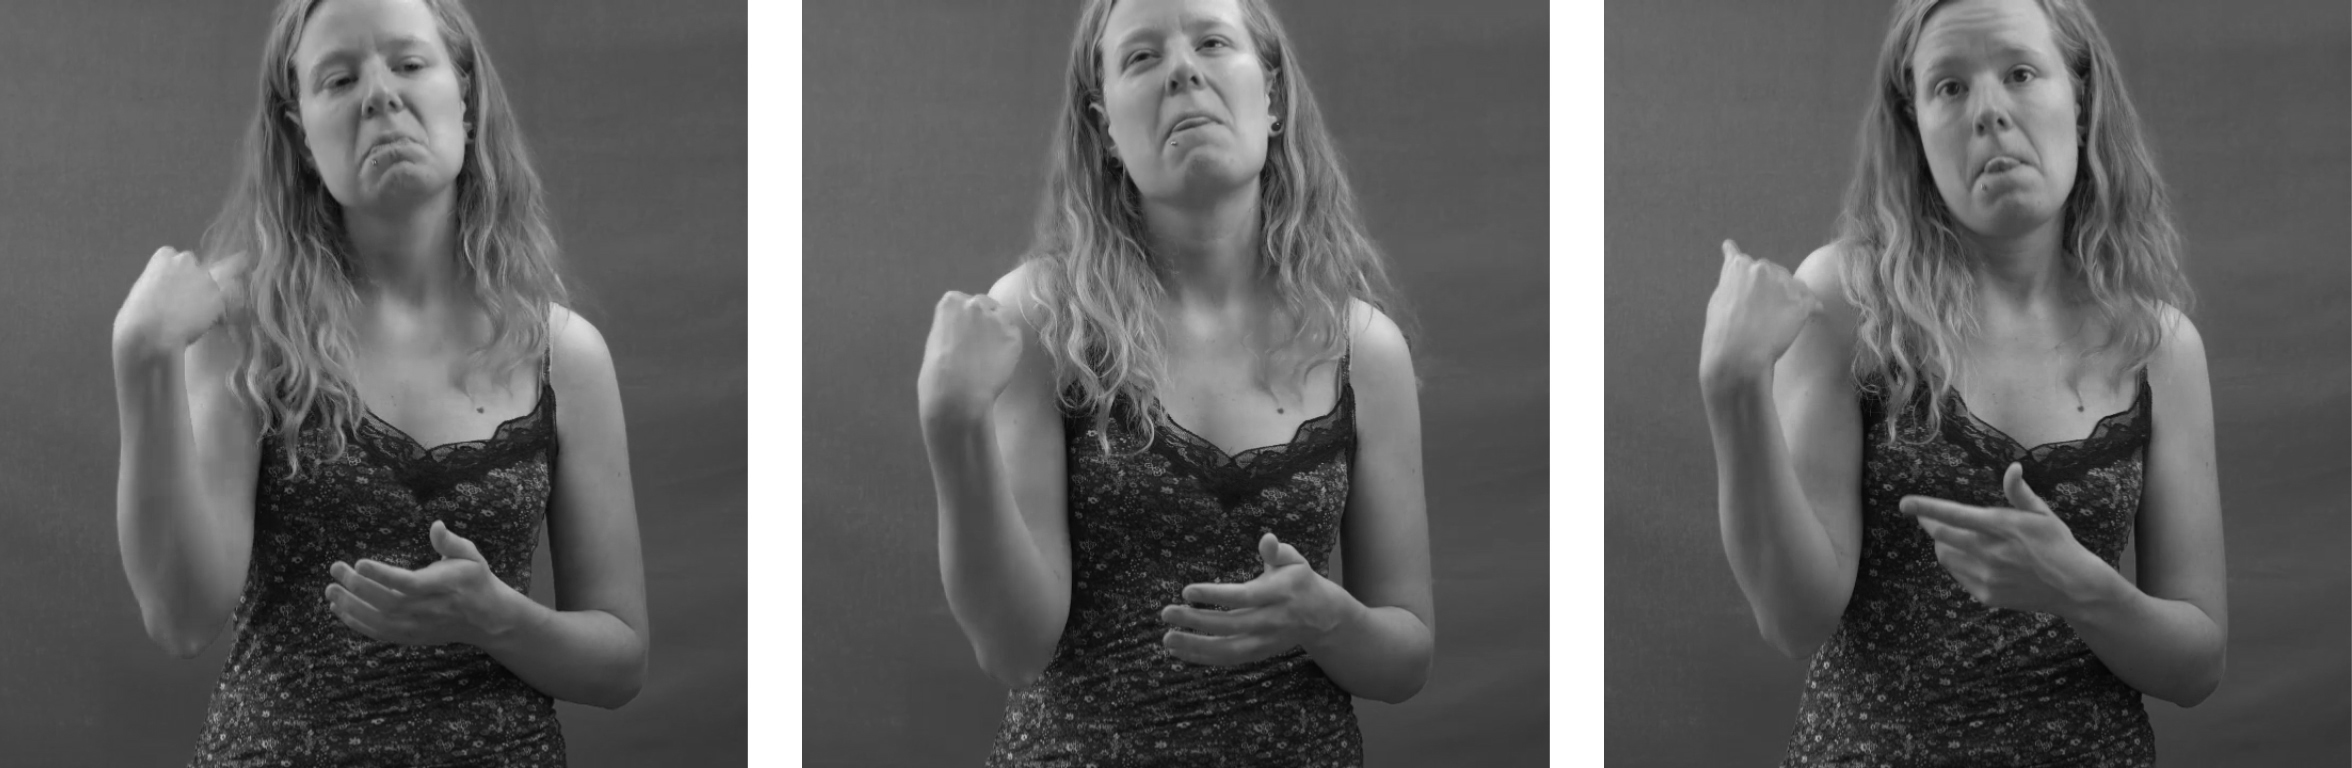
\includegraphics[width=1.0\textwidth]{just2sw.jpg}
	\caption{The non-manuals accompanying the sign \textsc{just}. The smaller the time interval is evaluated the stronger the non-manuals get.}
	\label{fig:just}
\end{figure}

Combining perfect and retrospective aspect in DGS leads to the expected patters, as shown in (\ref{retroretrodgstwo}).

\begin{exe}
\ex Context: When I visit Paul, he always has just taken a bath.\label{retroretrodgstwo}\begin{xlist} 
\ex \textcolor{white}{*}\slg{paul always} \slg[$==$]{just} \slg{bath}
\ex *\slg{paul} \slg[$==$]{just} \slg{always bath}
%\ex {} {\hspace{93pt}$= =$} {} \\
%\textcolor{white}{*}{\textsc{paul always}} {$\overline{\textrm{\textsc{just}}}$} {\textsc{bath}} 
%\glt \textcolor{white}{*}`Paul always just took a bath.' \label{ex:retroretrodgstwoa}
%\ex {} {\hspace{49pt}$= =$} {} \\
%{*\textsc{paul}} {$\overline{\textrm{\textsc{just}}}$} {\textsc{always bath}}
\glt \textcolor{white}{*}`Paul always has just taken a bath.' \label{ex:retroretrodgstwob}
\end{xlist}
\end{exe} 

\noindent The examples show that perfect aspect scopes higher than retrospective aspect in that the sign \textsc{always} has to precede the sign \textsc{just}. Taken together, retrospective aspect is expressed manually in DGS employing a left-to-right concatenation strategy. Although it is accompanied by a non-manual marker, this is the expression of a higher speaker-related category. It is worth noting that it can be argued that the non-manuals are an inherent part of the lexical entry for \textsc{just} and this may well be. However, as shown in Section \ref{scalarity}, there are signs allowing for both, the evaluation as little (by tensed lips or sucked-in cheeks) or the evaluation as much by inflated cheeks. In this case, it would be semantically odd not to evaluate \textsc{just} as being little, so the non-manuals make the impression of being an integral part of the sign. 

\is{retrospective aspect|(}

\section{Proximative aspect (\textit{soon})}\is{proximative aspect|(}
\subsection{General overview}
Proximative aspect is defined as an aspectual category marking ``nearness of completion of an action'' \citep[36]{heine1994genesis}. It thus marks that ``a temporal phase $[$is$]$ located close to the initial boundary of the situation described by the main verb'' (ibidem; emphasis changed). Instances of proximative aspect are adverbs of the type \textit{soon}. 

\subsection{The situation in DGS}
The adverb sign \textsc{soon} is signed manually and employs a left-to-right concatenation strategy, as shown in the examples in (\ref{proximativedgs}).

\begin{exe}
\ex \label{proximativedgs}\begin{xlist} 
\ex[] {{\textsc{paul soon apple++ buy}} 
\glt `Paul buys apples soon.' \label{ex:proximativedgsa}}
\ex[*] {{\textsc{paul apple++ buy soon}}
\glt `Paul buys apples soon.' \label{ex:proximativedgsb}}
\end{xlist}
\end{exe} 

\noindent Combining perfect and proximative aspect leads to the expected order perfect aspect $>$ proximative aspect, as shown by the examples in (\ref{perfectproximativedgs}).

\begin{exe}
\ex Context: Paul always wants to go swimming soon. In the end we never go. \label{perfectproximativedgs}\begin{xlist} 
\ex[] {{\textsc{paul wants always soon bath}} 
\glt `Paul always wants to go swimming soon.' \label{ex:perfectproximativedgsa}}
\ex[*] {{\textsc{paul wants soon always bath}}
\glt `Paul always wants to go swimming soon.' \label{ex:perfectproximativedgsb}}
\end{xlist}
\end{exe} 

\noindent Taken together, proximative aspect is expressed with the manual adverb \textsc{soon} that is concatenated from left to right, i.e., precedes the VP.
\is{proximative aspect|(}


\section{Durative aspect (\textit{briefly})}\label{durativeaspect}\is{durative aspect|(}
\subsection{General overview}
Durative aspect describes the duration of an event. \citet[41]{comrie1976aspect} states that ``durativity $[$\dots $]$ refers to the fact that the given situation lasts for a certain period of time'' and adds ``or at least, is conceived of as lasting for a certain period of time''. \citet[98]{cinque1999adverbs} notes that durative aspect is expressed by adverbs in English and has to be distinguished from adverbial PPs like \textit{for a while} or \textit{for an hour} which, according to him, do not appear in the specifier of the functional projection under discussion, but rather in the position of circumstantial adverbials. As an instance of durative aspect, Cinque names the adverb \textit{briefly}. 

Before discussing the data, it has to be noted that what is usually described as durative or continuative aspect in the literature on sign languages (e.g., \citealt{klima1979signs, wilbur2004event, rathmann2005event, happ2014vork}) finds its expression by altering the movement of the verb sign. This meaning will be discussed in Section \ref{durativecontinuative}.

\subsection{The situation in DGS}
Durative aspect is expressed manually in DGS and employs a left-to-right concatenation strategy, as illustrated in (\ref{durative}).

\begin{exe}
\ex\label{durative}\begin{xlist} 
\ex {\textcolor{white}{?}\textsc{paul briefly dance}} 
\glt \textcolor{white}{?}`Paul danced briefly.' \label{ex:durativea}
\ex {?\textsc{paul dance briefly}}
\glt \textcolor{white}{?}`Paul danced briefly.' \label{ex:durativeb}
\end{xlist}
\end{exe} 

\noindent A similar case is the adverb \textit{long}. It could be expected that the translational equivalent of \textit{long} in DGS would consist of a slow \is{reduplication}reduplication of the verbal sign. Instead, the manual sign \textsc{long} is used which itself is signed in a rather slow manner. Additionally, the verb sign can be performed in a slow way or, depending on its phonological form, be slowly reduplicated. I take this to be an expression of a structurally lower category discussed in Section \ref{durativecontinuative} indicating that a process continues longer than expected. This is shown in (\ref{ex:durativetwodgs}).


\begin{exe}
\ex {\textsc{yesterday paul poss\textsubscript{2} problem long report++}} 
\glt `Yesterday Paul told me about his problems for a long time.' \label{ex:durativetwodgs}
\end{exe} 

\noindent To conclude this section, durative aspect is expressed manually in DGS employing a left-to-right concatenation strategy. In addition, other means of modifying the movement of verb signs exist. I take these expressions to belong to a lower aspectual category as the quantification expressed does not refer to the event as a whole (in the last example, the event of Paul reporting his problems), but it rather seems as if they divide it into smaller sub-events. At this point, however, this is not totally clear yet (but see Section \ref{habitualtwo} and \ref{durativecontinuative} for evidence that the meaning produced by a manipulation of the movement path of the verb sign takes scope in a low position).
\is{durative aspect|)}

\section{Progressive aspect/Generic aspect (\textit{characteristically})}\label{characteristic}\is{progressive aspect|see{generic aspect}}\is{generic aspect|(}
\subsection{General overview}
\citet[99]{cinque1999adverbs} separates generic aspect and habitual aspect, although ``$[$g$]$e\-ner\-ic sentences are sometimes treated together with habitual sentences.'' He then cites \citet[97]{dahl1985tense} who states that habitual sentences ``differ from generic ones by their lack of lawlikeness.'' The unique feature of generic aspect is that it refers to a characteristic of an object that is inherent to this object. This inherent characterization does not necessarily find its realization. A simple English example is shown in (\ref{genericenglish}).

\begin{exe}
\ex This train travels 300 kilometers per hour. \label{genericenglish}
\end{exe} 

\noindent The sentence in (\ref{genericenglish}) can either refer to the speed of a train traveling 300 kilometers per hour at speech-time or it can refer to a general property of the train, namely that it generically is able to travel with this speed. Crucially, the train can be brand new and the generic sentence would still be fine -- even if the train has not traveled even a centimeter. 

\subsection{The situation in DGS}
As in English, generic aspect is left unexpressed in DGS. Thus, the sentence in (\ref{genericdgs}) can have a generic and a non-generic interpretation, just like the English example in (\ref{genericenglish}).


\begin{exe}
\ex {\textsc{index}\textsubscript{3a} \textsc{car 280 drive}} 
\glt `This car travels 280 kilometers per hour.'\label{genericdgs}
\end{exe} 

\noindent Optionally, habitual markers can be used that were described in Section \ref{habitualaspect} or the (root) modal verb \textsc{can} expressing an ability (see Section \ref{rootmodality}).


\is{generic aspect|(}

\section{Prospective (\textit{almost})}\is{prospective aspect|(}
\subsection{General overview}
Prospective aspect marks ``a point \textit{just prior} to the beginning of an event'' (\citealt[332]{frawley1992linguistic}, emphasis in original). With this, prospective aspect is a counterpart to retrospective aspect:

\begin{quote}
The perfect is retrospective, in that it establishes a relation between between a state at one time and a situation at an earlier time. If languages were completely symmetrical, one might equally well expect to find prospective forms, where a state is related to some subsequent situation, for instance where someone is in a state of being about to do something. \citep[64]{comrie1976aspect}
\end{quote}

\noindent Although not all languages are symmetrical in a way that they mark both aspects, there are languages in which prospective aspect is expressed via, for example, affixes (\citealt[99]{cinque1999adverbs} gives the example of Gungbe). As an instance of a semantically related adverb \citet[99]{cinque1999adverbs} mentions \textit{almost}.

\subsection{The situation in DGS}
This adverb is expressed manually in DGS, as shown in (\ref{prospective}). As illustrated in the example, \textsc{almost} employs a clear left-to-right concatenation strategy.\footnote{ A depiction of the adverb (in a different context) can be found in Figure \ref{fig:completivetwodgsexampletwo} on page \pageref{fig:completivetwodgsexampletwo}.}

\begin{exe}
\ex\label{prospective}\begin{xlist} 
\ex {\textcolor{white}{*}\textsc{paul almost apple buy}} 
\glt \textcolor{white}{*}`Paul almost bought an apple.' \label{ex:retrospectiveaa}
\ex {*\textsc{paul apple buy almost}}
\glt \textcolor{white}{*}`Paul almost bought an apple.' \label{ex:retrospectiveab}
\end{xlist}
\end{exe} 

\noindent Combining durative\is{durative aspect} aspect and prospective aspect gives the expected result (durative aspect $>$ prospective aspect), as illustrated in (\ref{durativeprospectivedgs}).

\begin{exe}
\ex Context: Recently, Paul almost reported his problems to me at length, but then the bus came and he couldn't even start. \label{durativeprospectivedgs}\begin{xlist} 
\ex {\textcolor{white}{*}\textsc{recently paul almost long poss\textsubscript{2} problem report++}} 
\glt \textcolor{white}{*}`Recently, Paul almost reported his problems to me at length.' \label{ex:durativeprospectivedgsa}
\ex {*\textsc{recently paul long almost poss\textsubscript{2} problem report++}}
\glt \textcolor{white}{*}`Recently, Paul almost reported his problems to me at length.' \label{ex:durativeprospectivedgsb}
\end{xlist}
\end{exe} 

\noindent Taken together, prospective aspect, again, is expressed by a manual-only left-to-right concatenation strategy.


\is{prospective aspect|)}
\section{Inceptive aspect I (\textit{begin})}\label{inceptiveoneaaa}\is{inceptive aspect I|(}
\subsection{General overview}
\citet{cinque1999adverbs, cinque2006restructuring} distinguishes between two inceptive aspects, one above and one below Voice. In both cases, the aspect refers to the starting point of an action. The higher aspectual category (inceptive aspect I) denotes a natural starting point while the lower one (inceptive II) denotes an arbitrary starting point. Thus an example of inceptive I would be \textit{to start to build a house} and an example of inceptive II \textit{to start to shiver}. Note that inceptive I and inceptive II also differ in that inceptive I always involves an agent while inceptive II the subject is non-volitional (i.e., unaccusative). From the examples it is clear that inceptive I should be located in a projection above VoiceP (in which the agent is introduced) and inceptive II should be located in a projection below VoiceP. Inceptive aspect II will be discussed in Section \ref{inceptivetwo} (see page \pageref{inceptivetwo}).

\subsection{The situation in DGS}
Inceptive aspect I is expressed with the verb \textsc{begin}. This verb needs to be expressed by way of a left-to-right concatenation strategy, as shown in (\ref{inceptiveone}).

\begin{exe}
\ex  \label{inceptiveone}\begin{xlist} 
\ex {\textcolor{white}{?}\textsc{paul begin house building}} 
\glt \textcolor{white}{?}`Paul started to build a house.' \label{ex:inceptiveonea}
\ex {?\textsc{paul house building begin}}
\glt \textcolor{white}{?}`Paul started to build a house.' \label{ex:inceptiveoneb}
\end{xlist}
\end{exe} 

\noindent This is a rather unexpected result as other verbs that appear in verb-verb combinations, like the manual modals, \textsc{try}, or \textsc{manage} (see the next section), seem to have more positional freedom.

\is{inceptive aspect I|(}
\section{Success aspect (\textit{manage})}\is{success aspect|(}
\subsection{General overview}
Success aspect, represented by \textit{manage} in \citet{cinque1999adverbs, cinque2006restructuring}, is an aspect related to the successful accomplishment of an action. It is located by Cinque in the same position as frustrative aspect\is{frustrative aspect|see{success aspect}}. 

\subsection{The situation in DGS}
The DGS verb \textsc{manage} behaves similar to the verb \textsc{try} representing conative aspect in Cinque's system. As with \textsc{try}, \textsc{manage} rather behaves like a modal or volitional verb (see the discussion of conative aspect in Section \ref{conative}) and appears either in a pre- or post-verbal position, as shown in (\ref{successaspectchild}).

\begin{exe}
\ex  \label{successaspectchild}\begin{xlist} 
\ex {\textsc{paul manage child lift}} 
\glt `Paul managed to lift the child.' \label{ex:successaspecta}
\ex {\textsc{paul child lift manage}}
\glt `Paul managed to lift the child.' \label{ex:successaspectb}
\end{xlist}
\end{exe} 

\noindent In contrast to \textsc{begin} (discussed in the previous section), the verb \textsc{manage} behaves more like a modal verb, as it exhibits more positional freedom. This is corroborated by the fact that \textsc{manage} can be, just like other modal verbs, doubled, as shown in (\ref{ex:successaspectclift}).

\begin{exe}
\ex {\textsc{paul manage child lift manage}}
\glt `Paul managed it to lift the child.' \label{ex:successaspectclift}
\end{exe} 

\noindent In addition, just like other modal verbs, \textsc{manage} is negated by alpha-negation, i.e., by changing the movement path of the verb sign instead of employing a non-manual strategy only (i.e., by shaking the head).
\is{success aspect|(}

\largerpage[1.5]
\section{Root modality (\textit{being able})}\label{rootmodality}\is{root modality|(}
\subsection{General overview}
The term `root modality' is usually used as a cover term for a modality that ``expresses necessity, obligation, permission, volition, or ability on behalf of an agent which usually, but not necessarily, is expressed by the [\dots ] subject of the sentence'' \citep[44]{platzack1979semantic}. In many languages each of the mentioned functions has its own lexical item and in many languages each of the functions leads to different morpho-syntactic reflexes (e.g., \citealt{bross2017swabian}). I will take that as an indication that they constitute different categories. With the term `root modality' I will refer only to the ability of a subject-agent or to a property of a subject in the case of an inanimate referent (hence, there is only root possibility and no root necessity). Examples for root modality according to this definition are given in (\ref{rootexamples}).

\begin{exe}
\ex\label{rootexamples}\begin{xlist}
\ex Miraculix can perform magic (i.e., he is able to perform magic).
\ex (The soil is good.) Flowers can grow here.
\end{xlist}
\end{exe}

\subsection{The situation in DGS}
\noindent Root modality is expressed most naturally with clause-final modal verbs in DGS (for an overview, see also \citealt{pfauquer2007syntaxofnegationandmodals}). This is shown in (\ref{rootmodalitydgsexamples}). The example in (\ref{bsp:happhapphapp}) is taken from \citet[359]{happ2014vork} and the example in (\ref{bsp:glosserrrqcsbeta}) from \citet[23]{bross2017scope} (the gloss `() ()' indicates puffed cheeks).

\begin{exe}
\ex\label{rootmodalitydgsexamples}\begin{xlist}
\ex\label{bsp:happhapphapp}
{}   
{\textsc{miraculix perform-magic can}}    
\glt `Miraculix can perform magic.' 

\ex\label{bsp:glosserrrqcsbeta}
\slg{soil} \slg[() ()]{good} \slg{flowers grow can}
%{} {\hspace{37pt}() ()} {} {}  \\
%{\textsc{soil}} {$\overline{\text{\textsc{good}}}$} {\textsc{flowers grow}} {\textsc{can}}     
\glt `The soil is rich, flowers can grow here.' 
\end{xlist}
\end{exe}

\noindent As with other uses of modal verbs, the position of the root modals seems to be subject to variation in DGS. As already noted in \citet[23]{bross2017scope}, the modal can also appear in a pre-verbal position shown in (\ref{bsp:ungramma}). In such cases, however, the construction is used to indicate narrow focus/contrastive stress on the modal.

\begin{exe}
\ex {\textsc{miraculix can perform-magic}}   \label{bsp:ungramma} 
\glt *\phantom{\cmark} `Miraculix can perform magic.' \\
\cmark\phantom{*} `Miraculix \textsc{can} perform magic.'
\end{exe}

\largerpage
\noindent However, on closer inspection, many signers do not share this intuition. There is, nevertheless, an indication that the base position of root modals is post-verbal, namely the behavior of multi-modal constructions. When a root modal is combined with a volitional modal, the only acceptable order is one in which the volitional modal is in a pre- and the root modal in a post-verbal position. In other words, when modals from a higher syntactic position are combined with modals from a syntactically lower position, the order of scope-taking must be obeyed (in other words: the modals need to be in their base positions). This is shown in the examples in (\ref{calculation}).

\begin{exe}
\ex Context: Maria is able to calculate very well.\label{calculation}\begin{xlist}
\ex\label{bsp:calculatea}
%{}   
{\textcolor{white}{*}\textsc{otto want also well calculate can}}    
\glt \textcolor{white}{*}`Otto also wants to be able to calculate well.' 

\ex\label{bsp:calculateb}
%{}   
{*\textsc{otto can also well calculate want}}    
\glt \textcolor{white}{*}`Otto also wants to be able to calculate well.' 

\end{xlist}
\end{exe}

\noindent To conclude, there is much variation as to the position of root modals, just as with other manual modals. However, there is some evidence in favor of the position that root modals occupy a post-verbal rather than a pre-verbal base position. 


\is{root modality|(}
\section{A note on modal doubling}\label{modaldoubling}
\is{focus doubling|(}
It has often been noted in the literature that many sign languages allow the doubling of modal signs (beside the doubling of quantifiers, personal pronouns etc.) and it has often been assumed that one of the modals is in a focus position (for an overview of doubling, see \citealt{petronio1993clause,nunesquadros2008phonetically}).

German Sign Language allows modal doubling as well. Similar to other doubling constructions in DGS, many signers claimed that this construction is not frequently used. Nevertheless, many of them spontaneously produced doubling of all sorts in other contexts. This discrepancy between conscious judgments and actual use is reflected in the inter-signer variability of which constructions were accepted and which were not. To note just a few variations: some signers accepted the doubling of negated modals while others did not. Among the three signers accepting negated modal doubling, two did not like doubling of \textsc{want-neg} while one did. In this area, more systematic research is clearly needed. For the moment, I will concentrate on those instances of modal doubling that were accepted by all signers.

As already noted in the last section, root modals naturally occur in a post-verbal position (\ref{ex:doublinga}) and can receive narrow focus in a pre-verbal position (\ref{ex:doublingb}). This analysis may sound simple, but it is bedeviled by the fact that it is possible to add a focus marker (produced with the head and the eyebrows) onto the modal both in a pre- and post-verbal position. Additionally, root modals can be doubled (\ref{ex:doublingc}). 

\begin{exe}
\ex\begin{xlist} 

%\glll {}
%{} {\hspace{343pt}}  \\
\ex {\textsc{paul perform-magic can}}
\glt `Paul can perform magic.' \label{ex:doublinga}
\ex {\textsc{paul can perform-magic}}
\glt `Paul can perform magic.' \label{ex:doublingb}
\ex \slg{paul can perform-magic} \slg[foc]{can}
%\ex {} {\hspace{158pt}foc}  \\
%{\textsc{paul can perform-magic}} {$\overline{\textrm{\textsc{can}}}$} %\\
\glt `Paul \textsc{can} perform magic.' \label{ex:doublingc} 

\end{xlist}
\end{exe} 

\noindent In the case of doubling, it is the post-verbal modal which receives focus marking -- regardless of modal flavor. Figure \ref{fig:modaldoubling} shows two examples of modal doubling. The top example shows doubling of the volitional modal \textsc{want} with the clause-final instance of the modal being focus-marked. The bottom example shows an example with the root modal \textsc{can}. The focus marking in this case is more subtle.

\is{focus doubling|)}


\begin{figure}[h]
\centering
	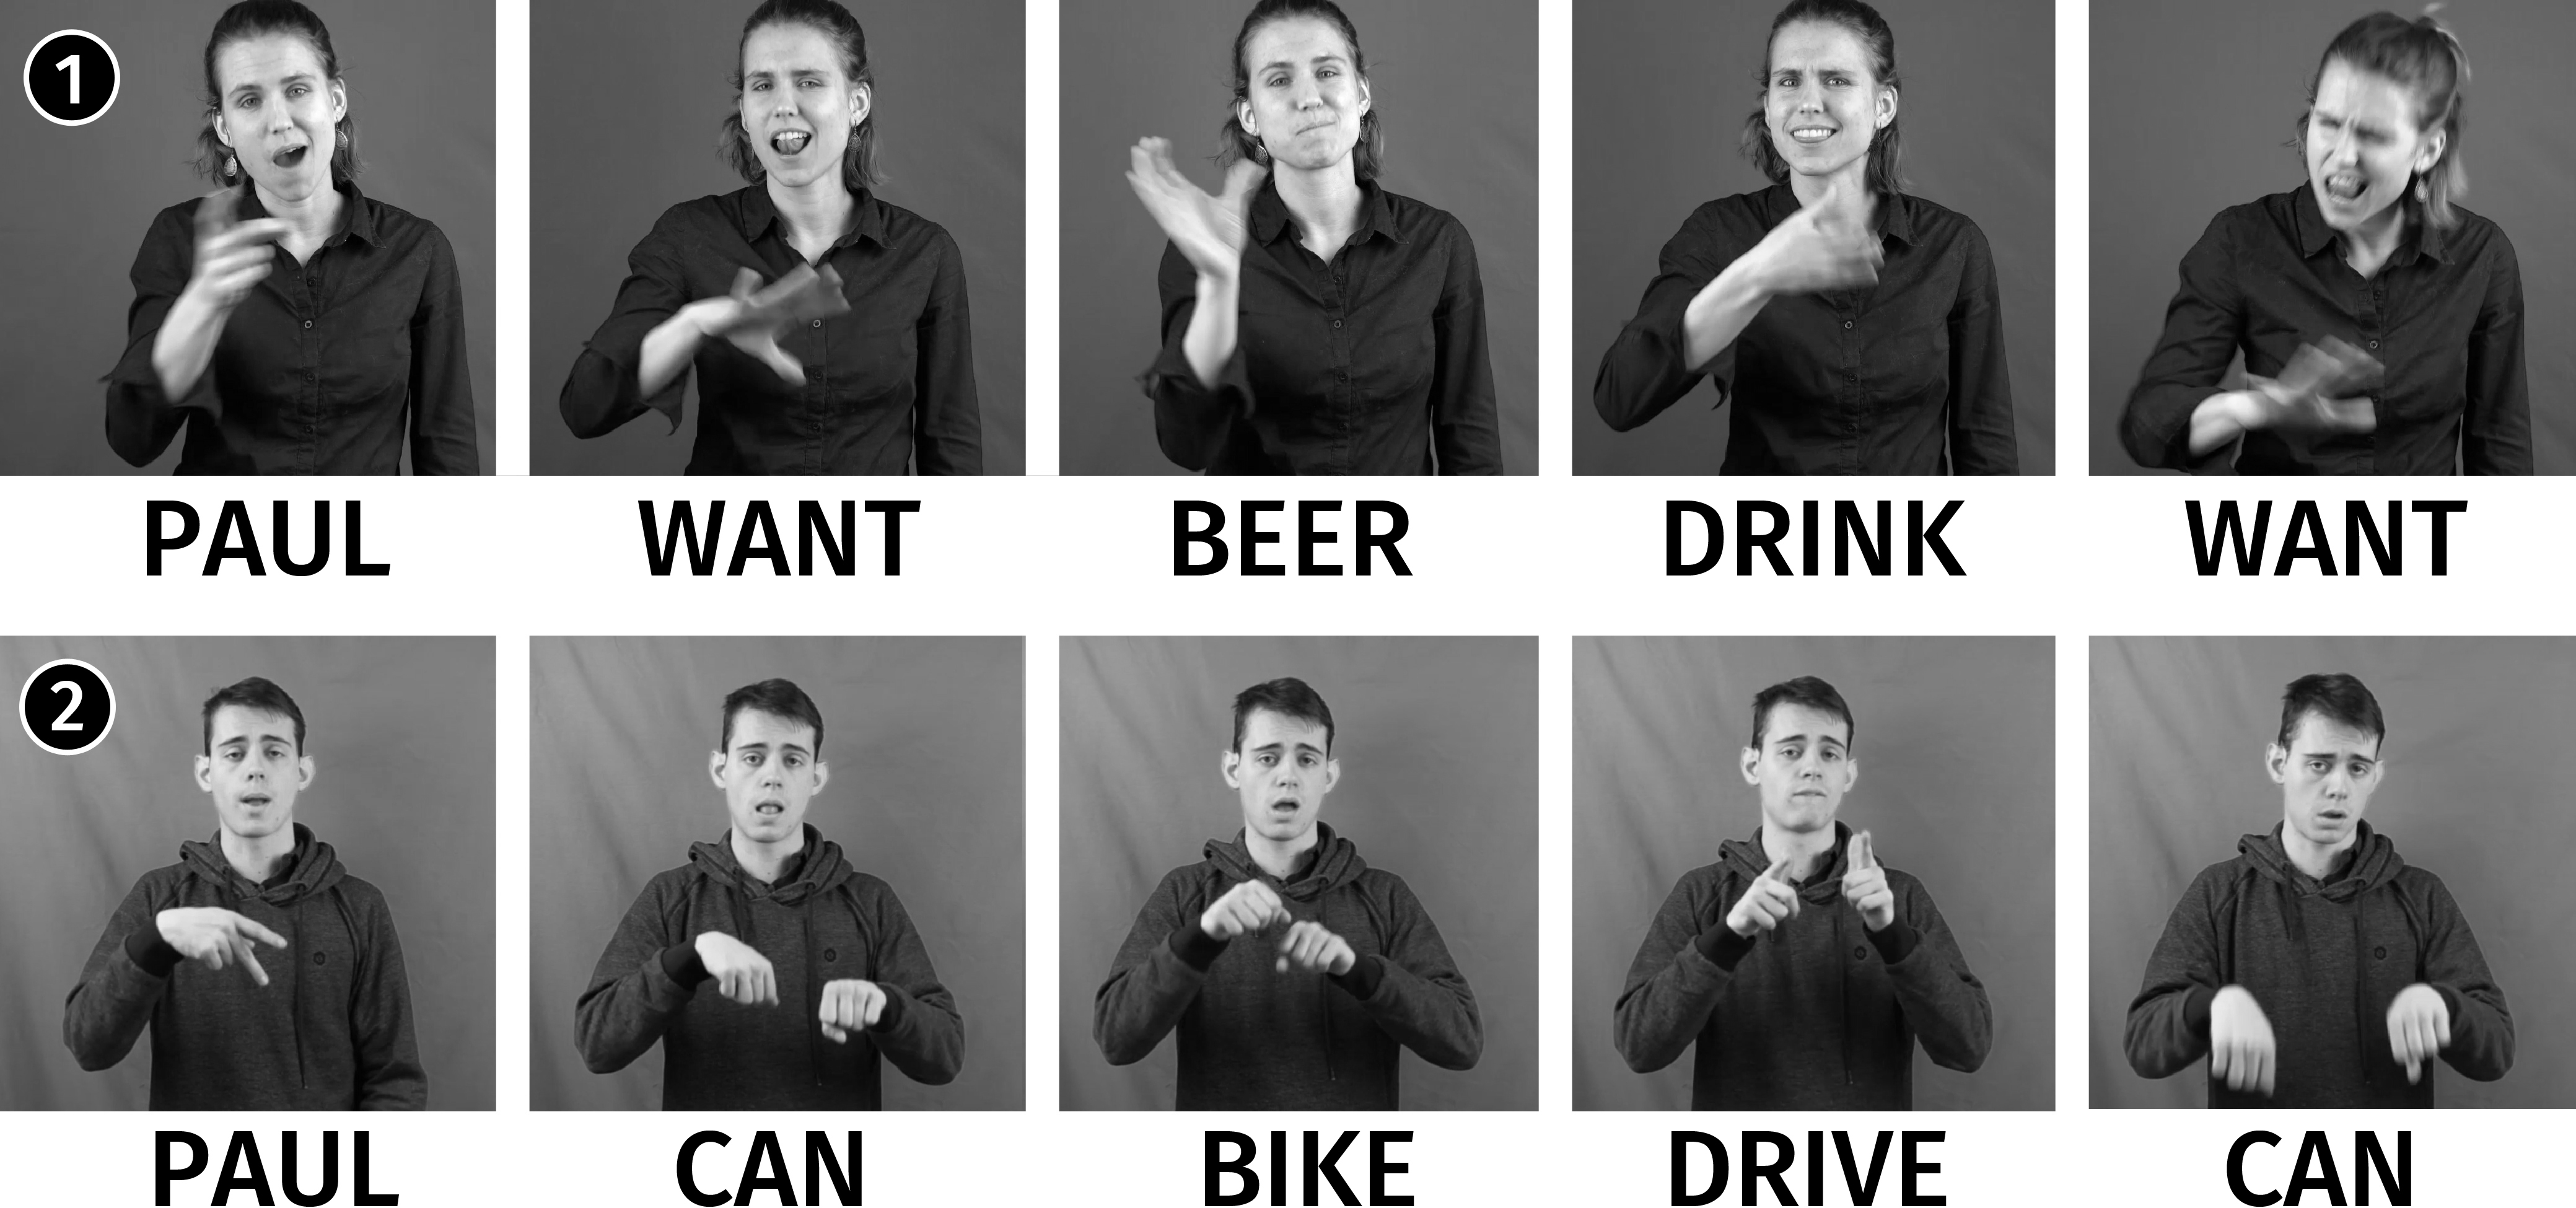
\includegraphics[width=1.0\textwidth]{modaldoublingsw.jpg}
	\caption{The post-verbal modal in modal-doubling construction is obligatorily focus-marked by a head nod and brow-lowering (the nod may be rather strong as in the top sentence labeled 1 or rather subtle as in the bottom sentence labeled 2).}
	\label{fig:modaldoubling}
\end{figure}



\largerpage
\section{Conative aspect (\textit{try})}\label{conative}\is{conative aspect|(}
\subsection{General overview}
Conative aspect, discussed by \citet{cinque1999adverbs, cinque2006restructuring} only very briefly, is defined as the marking of ``the fact that a certain action may take some effort'' \citep[105]{cinque1999adverbs}. As an example, he uses \textit{try-to}-constructions. Cinque's definition is somehow misleading as it suggests a manner reading. \citet[568]{signgram2017} in the SignGram Blueprint define conative aspect as expressing ``the meaning of trying to do something (and not necessarily succeeding)'' and as signalling ``that someone is trying to do something with the implication that the event is about to occur, usually not yet finished, thus imperfective, and that in most cases the activity won't be finished in the future'' \citep[225--226]{signgram2017}. The notion of conative aspect has been used in the sign language literature in different ways. For \is{American Sign Language}American Sign Language, for example, it was used to describe what is sometimes labeled `unrealized inceptive'. This aspectual category is used to express that someone did not do something, but was about to do it (paraphrased by \textit{almost} by \citealt{wilbur2010semantics}). This is signed by interrupting the movement of the verb sign and holding the hand configuration for a short time at that point \citep{liddell1984unrealized, rathmann2005event}. This is, of course, only possible for certain verbs, namely for the class of verbs with telic meanings (for \is{telicity}telicity, conative aspect, and unrealized inceptive see also \citealt{wilbur1987american, brentari1998prosodic, wilbur2008complex, wilbur2010semantics}).

Given the diversity of meanings that conative aspect has, I will just briefly describe the situation for DGS and leave a more fine-grained analysis to future research. Taking Cinque's definition of conative aspect seriously, in that it marks that an action may take some effort, we indeed find an expression in DGS involving a change of the movement path of a sign. To be more precise, the verb sign is signed more slowly, sometimes with a more curvy path and non-manuals expressing effort are employed. By observing Cinque's examples of conative aspect, for example the one in (\ref{ex:cinqueconative}) from \citet[143]{cinque2001restructuring}, it seems unlikely that he was after the (structurally probably rather low) manner reading.

\begin{exe}
\ex \gll {\textit{Gianni}} {\textit{le}} {\textit{continuó}} {\textit{a}} {\textit{provare}} {\textit{a}} {\textit{telefonare}} \\
{Gianni} {her} {continued} {to} {try} {to} {call} \\
\trans `Gianni continuously tried to call her.' \label{ex:cinqueconative}
\end{exe} 

\subsection{The situation in DGS}
\noindent Concerning the expression of the unrealized inceptive in DGS, I have found mixed evidence that it is possible to stop the movement path of a sign and to hold the hand configuration. Some signers clearly rejected this as a possible construction in DGS, others, however, rated it as possible. However, when asked to translate a sentence with a \textit{try} context all used the verb \textsc{try}.


Concerning the verb \textsc{try}, that was said to be more a volitional or modal category than an expression of conative aspect \citep[568]{signgram2017}, we find a manual expression in DGS. Its preferred position to the left or to the right of the VP seems to be subject to inter-signer variation, although both positions were judged to be equally acceptable. This is illustrated in the examples in (\ref{ex:conativedgsa}) and (\ref{ex:conativedgsb}). 

\begin{exe}
\ex  \label{conativedgs}\begin{xlist} 
\ex {\textsc{paul book read try}} 
\glt `Paul tries to read the book.' \label{ex:conativedgsa}
\ex {\textsc{paul try book read}}
\glt `Paul tries to read the book.' \label{ex:conativedgsb}
\end{xlist}
\end{exe} 

\noindent Constructions with the verb \textsc{try} were even produced with verbs that have a clear on- and offset, both conceptually as well as phonologically. An example of such a verb is \textsc{lift}, shown in (\ref{conativedgsaab})

\begin{exe}
\ex  \label{conativedgsaab}\begin{xlist} 
\ex {\textsc{paul child lift try}} 
\glt `Paul tries to lift the child.' \label{ex:conativedgsaa}
\ex {\textsc{paul try child lift}}
\glt `Paul tries to lift the child.' \label{ex:conativedgsbb}
\end{xlist}
\end{exe} 

\noindent Taken together, the verb \textsc{try} behaves like a modal verb in that it allows both for a pre- and a post-verbal position. It thus seems that verbs in verb-verb constructions in DGS in general allow more positional freedom compared to adverb placement.
\is{conative aspect|(}

\largerpage
\section{Completive aspect I (\textit{completely})}\label{completiveone}\is{completive aspect I|(}
\subsection{General overview}
Completive aspect I ``marks the termination of a bounded process at its natural end point: `finish'\,'' \citep[70]{cinque2006restructuring}. \citet[100--104]{cinque1999adverbs} additionally distinguishes completive aspect II which he locates below Voice. For completive I, \citet{cinque1999adverbs} distinguishes two subcategories, singular and plural completion. For singular completion, \citet[100]{cinque1999adverbs} states:

\begin{quote}
With a telic\is{telicity} process like `eating the sandwich', the natural end point is reached when the object has been totally affected (when there is no residue left of the sandwich). In English, this can be explicitly signaled with the particle \textit{up} (\textit{He ate up his sandwich}, \textit{Eat up your sandwich!})[\dots ].
\end{quote}

\noindent Plural completion in contrast is about a set of entities. Each member of the set has been affected and, as in singular completion, each member of the set has been completely affected. So in an example like \textit{He ate up the sandwiches}, the set of sandwiches talked about is completely affected and each individual sandwich has been consumed completely. This distinction goes back to \citet[57--69]{bybee1994evolution}. 

These two completive aspects (the singular and the plural one) are, according to \citet{cinque1999adverbs} above his Voice projection. Completive II he considers to be below Voice, but it is not entirely clear what he means by completive aspect II. One lead to what the distinction refers to is given in a footnote in \citet[178]{cinque1999adverbs} in which he compares

\begin{quote}
the adverb \textit{completely} in its preverbal and postverbal positions: \textit{John completely forgot her instructions} versus \textit{John forgot her instructions completely}. The second sentence is ambiguous. It can mean either that John forgot every part of each of her instructions or that they did not occur to him at the appropriate moment. [\dots ] The first has only the latter reading.
\end{quote}


\noindent In \citet[69]{cinque2006restructuring}, however, he claims that ``$[$o$]$ne instance of completive aspect (`terminate a process at its natural ending point', `finish') is crucially lower than Voice''. From the discussion of completive aspect in \citet{cinque2006restructuring}, it seems that the exact location of the two or three different types of completive aspect is not totally settled. 

I will take the view that the completion of sets refers to a higher aspectual category and the completion of a process is an instance of a lower aspectual category that is inside the VoiceP (i.e., an inner aspect). Note that the term `completive aspect' is often used to refer to the use of signs of the sort \textsc{finish}. This kind of expression will be discussed in a side-note on page \pageref{exkursfertigdurch}.

\subsection{The situation in DGS}
Plural completion is marked in DGS, however, not by a single adverb, but rather by introducing several referents into the signing space as illustrated in Figure \ref{fig:completiveonedgs}. This, however, does not tell us anything about the syntactic position of a higher completive projection. 


\begin{figure}[bt]
\centering
	
\includegraphics[width=1.0\textwidth]{completivesw.jpg}
	\caption{Plural completion is marked by distributing three referents in the signing space. This is achieved by locating them via indices (glossed as \textsc{index}\textsubscript{\textsc{loc}}). The example translates: \textit{Paul ate from each sandwich}. The black bar indicates that \textsc{index\textsubscript{loc}} is one sign that is depicted using several images.}
	\label{fig:completiveonedgs}
\end{figure}

Another candidate for a higher completive projection is the manual adverb \textsc{completely}. An example is shown in (\ref{ex:completelyinstructions}). 

\begin{exe}
\ex {\textsc{paul instruction completely forget}} 
\glt `Paul forgot the instructions completely.' \label{ex:completelyinstructions}
\end{exe} 

\noindent The sentence in (\ref{ex:completelyinstructions}) indeed only has the reading of the adverb that is located in a higher position in English (see the quote by \citealt[178]{cinque1999adverbs} above). However, more research, in the area of completive aspect in general as well as its expression in DGS, is needed.

\is{completive aspect I|(}




\section{Voice/Manner (\textit{well})}\is{Voice}\is{manner|(}

\subsection{General overview}
\citet[101--102]{cinque1999adverbs} assumes that light manner adverbs (e.g., \textit{well}) are located in the specifier position of the Voice head. As I take this position, following \citet{kratzer1996severing}, to be the one in which the agent is introduced in the structure I suggest splitting up the tree at this point and assuming a MannerP in which (light) manner adverbs are located. It is somewhat controversial where exactly in the syntax one could locate manner adverbs of the kind discussed in this section. For some, manner adverbs are structurally higher than VoiceP (e.g., \citealt{alexeyenko2012manner}; \citealt{cognola2013mixed}), while for others the position is flexible, either within one language (e.g., \citealt{haumann2007adverb}) or across languages (e.g., \citealt{kahnemuyipour2009syntax}). 

\subsection{The situation in DGS}
Manner adverbs like \textsc{well} are expressed manually using a more or less clear right-to-left concatenation strategy in DGS as exemplified in the examples in (\ref{mannerwelldgs}). Note that this pattern would be hard to explain assuming that \textsc{well} is located in SpecVoiceP which I assume to be left in DGS.

\begin{exe}
\ex\label{mannerwelldgs}\begin{xlist}
\ex \textcolor{white}{\%}\textsc{kassandra dance well} 
\glt \textcolor{white}{\%}`Kassandra is dancing well.' \label{mannerwelldgsa}
\ex \%\textsc{kassandra well dance} 
\glt \textcolor{white}{\%}`Kassandra is dancing well.' \label{mannerwelldgsb}
\end{xlist}
\end{exe}

\largerpage
\noindent The reason why the example in (\ref{mannerwelldgsb}) in which the manner adverb is found in a pre-verbal position is marked with a percent sign instead of an asterisk is because some signers allow for this position. Nevertheless, most of my consultants found this construction a little bit marked.


This fits in well with the observations made in the literature on DGS. \citet[282]{happ2014vork} for example, give the following example of a post-verbal manual adverb.

\begin{exe}
\ex \textsc{woman write, nicely}
\glt `The woman writes in a nice way.'
\end{exe}

\noindent The reason for the comma in their glossing is their claim that there is a short intonational break between the verb and the adverb. From my own observations it seems as if this pause is not necessary, but I will leave this point open for further investigation.

In summary, the category discussed by \citet{cinque1999adverbs} under the label `Voice' is expressed manually in DGS.  Its natural position in DGS is post-verbal, so I take this category as being expressed by a right-to-left concatenation strategy.

\is{manner|(}


\section{Summary and conclusion}
This chapter started with a discussion of the highest categories in Cinque's hierarchy, i.e., those above the tense projection. It was shown that all these categories (speech-act-indicating expressions, mirative, evaluation, evidential, epistemic, and scalarity) are expressed via non-manual markings and, optionally, with a manual marker plus the respective non-manuals. When a manual element is present, the non-manuals are not as strong as when the non-manual-only strategy is chosen. In contrast to the non-manuals used to express categories of the higher CP that were discussed in the previous chapter, the non-manuals marking the lower portion of the CP spread from left-to-right (and not from right-to-left), i.e. the intensity of the non-manuals is strongest at the beginning of the clause. As the intensity peak of non-manual marking was taken to be an indication of the syntactic origin of the respective heads that trigger these markings (\citealt{bahan1996}; \citealt{petronio1997}; \citealt[43--45]{neidle2000syntax}; \citealt[311--312]{sandler2006sign}), it can be hypothesized that these categories are left-headed (although I think that this claim, in general, is in need of more empirical evidence). As, additionally, the manual adverbs that can be used for the expression of the high categories in this domain have a strong tendency to appear clause-initially, it can be stated that the respective projections are also left-branching. I thus arrived at the representation shown in (\ref{ex:lowercp}), repeated here as (\ref{ex:lowercpv}). Note that scalarity is left out as this category behaves differently.


For the two categories directly below Tense, Cinque's irrealis mood and alethic modality, I have argued that both scope above Tense. In both cases the data presented suggests that they are either special instances of epistemic modality or that they at least belong to categories that show syntactic behavior very similar to epistemic modality.

All the higher categories which are expressed non-manually (i.e., the categories above tense) contribute not-at-issue meaning. While more research in this area is highly welcomed, my preliminary data suggests that the Cinquean categories above tense are not-at-issue when expressed non-manually only, but are at-issue when expressed by a manual plus non-manual strategy. This indicates that there is a meaning difference between adverbs in, for example, English, in which the higher adverbs contribute not-at-issue meaning, and adverbs in DGS. The conclusion to draw from this is that non-manual expressions (at least in the relevant portion of the clausal spine) are not-at-issue in general, while manual expressions are generally at-issue. Obviously, there are exceptions to this generalization as movements of the whole head are excluded. Negation, for example, is expressed non-manually by a head shake in DGS and negation, of course, is at-issue. Future research will also need to take lexical non-manuals (see \citealt{pendzich2017lexicalnmms}) into account and check whether these also contribute not-at-issue meanings.


\begin{exe}
\ex \label{ex:lowercpv}
\begin{forest}
for tree={s sep=3.8mm, inner sep=0, l=10mm} %s sep = Breite; l = Höhe
[SpeechActP [{\phantom{NNN}} ] [{$\overline{\textrm{SpeechAct}}$} [{SpeechAct\textdegree } ] [MirativeP [.{\phantom{NNN}} ] [{$\overline{\textrm{Mirative}}$} [{Mirative\textdegree } ] [EvaluativeP [.{\phantom{NNN}} ] [{$\overline{\textrm{Evaluative}}$} [{Evaluative\textdegree } ] [EvidentialP [{\phantom{NNN}} ] [{$\overline{\textrm{Evidential}}$} [{Evidential\textdegree } ] [EpistemicP [.{\phantom{NNN}} ] [{$\overline{\textrm{Epistemic}}$} [{Epistemic\textdegree } ] [{\phantom{NNN}} ] ] ] ] ] ] ] ] ] ] ]
\end{forest}
\end{exe}

%\begin{exe}
%\ex \label{ex:lowercpv}
%\begin{tikzpicture}[baseline=(current bounding box.north), scale=0.90]
%\tikzset{level distance = 28pt, sibling distance=1pt}
%\tikzset{every tree node/.style={align=left,anchor=north}}
%\Tree [.SpeechActP [.{} ] [.{$\overline{\textrm{SpeechAct}}$} [.{SpeechAct\textdegree } ] [.MirativeP [.{} ] [.{$\overline{\textrm{Mirative}}$} [.{Mirative\textdegree } ] [.EvaluativeP [.{} ] [.{$\overline{\textrm{Evaluative}}$} [.{Evaluative\textdegree } ] [.EvidentialP [.{} ] [.{$\overline{\textrm{Evidential}}$} [.{Evidential\textdegree } ] [.EpistemicP [.{} ] [.{$\overline{\textrm{Epistemic}}$} [.{Epistemic\textdegree } ] [.{} ] ] ] ] ] ] ] ] ] ] ]
%\end{tikzpicture}
%\end{exe}

Concerning the expression of modal categories below epistemic modality, i.e. deontic modality, volition, and root modality, it has been observed that the position of the manual modals is rather free. It was claimed that this has to do with the fact that verbs are heads instead of phrases. That the positional freedom has something to do with the fact that they are verbs fits in well with the observation made, for example, in Section \ref{volition} that the same freedom was not observed with semantically related adverbs (e.g., the volitional modal \textsc{want} can appear in a pre- as well as in a post-verbal position, but the same was not true for the manual adverb \textsc{intentionally}). Additionally, inserting an adverb into a sentence containing a modal verb opens up not two, but three different positioning possibilities. This was shown in the examples in (\ref{modalhabitualb}), repeated here as (\ref{modalhabitualbcc}).

\begin{exe}
\ex\label{modalhabitualbcc}\begin{xlist} 
\ex \textsc{paul usually early at-home-be must}
\glt `Usually, Paul must be at home early.'
\ex \textsc{paul usually must early at-home-be}
\glt `Usually, Paul must be at home early.'
\ex \textsc{paul must usually early at-home-be}
\glt `Usually, Paul must be at home early.'
\end{xlist}
\end{exe} 

\noindent Assuming that the adverb \textsc{usually} occupies a specifier position, this behavior is actually expected. The modal verb \textsc{must} can move to different head positions. Thus, the examples in (\ref{modalhabitualbcc}) are analogous to the examples (\ref{finiteauxcinque}) discussed by \citet[49]{cinque1999adverbs}, repeated here as (\ref{finiteauxcinqueq}). 

\begin{exe} 
\ex Italian \citep[49]{cinque1999adverbs}\label{finiteauxcinqueq} \begin{xlist} 
\ex \gll {Mi ero} {\textit{francamente}} {\textit{purtroppo}} {\textit{evidentemente}} {\textit{formato}} {\textit{una}} {\textit{pessima}} {\textit{opinione}} {\textit{di}} {\textit{voi}.}  \\
{Me be-1-\textsc{sg}} {frankly} {unfortunately} {clearly} {formed} {a} {bad} {opinion} {of} {you} \\
\trans `Frankly, I unfortunately had clearly a formed a very bad opinion of you.' \label{finiteauxcinqueaq}

\ex \gll  {\textit{Francamente}} {mi ero} {\textit{purtroppo}} {\textit{evidentemente}} {\textit{formato}} {\textit{una}} {\textit{pessima}} {\textit{opinione}} {\textit{di}} {\textit{voi}.}  \\
 {Frankly} {me be-1-\textsc{sg}} {unfortunately} {clearly} {formed} {a} {bad} {opinion} {of} {you} \\
\trans `Frankly, I unfortunately had clearly a formed a very bad opinion of you.' \label{finiteauxcinquebq}

\ex \gll  {\textit{Francamente}}  {\textit{purtroppo}} {mi ero} {\textit{evidentemente}} {\textit{formato}} {\textit{una}} {\textit{pessima}} {\textit{opinione}} {\textit{di}} {\textit{voi}.}  \\
 {Frankly}  {unfortunately} {me be-1-\textsc{sg}} {clearly} {formed} {a} {bad} {opinion} {of} {you} \\
\trans `Frankly, I unfortunately had clearly a formed a very bad opinion of you.' \label{finiteauxcinquecq}

\ex \gll  {\textit{Francamente}}  {\textit{purtroppo}}  {\textit{evidentemente}} {mi ero} {\textit{formato}} {\textit{una}} {\textit{pessima}} {\textit{opinione}} {\textit{di}} {\textit{voi}.}  \\
 {Frankly}  {unfortunately}  {clearly} {me be-1-\textsc{sg}} {formed} {a} {bad} {opinion} {of} {you} \\
\trans `Frankly, I unfortunately had clearly a formed a very bad opinion of you.' \label{finiteauxcinquedq}

\end{xlist} 
\end{exe}

\noindent While the ordering possibilities among modals and adverbs was shown to be free, the ordering of several modals in one clause, in contrast, was found to be very restricted. To be more precise, combining two modals in one clause leads to the expected structures. Combining a volitional and a root modal, for example, was shown in Section \ref{rootmodality} to result in the order volitional modal $>$ root modal and not the other way around.

Concerning the adverbs discussed in this chapter, it was found that they all find manual expression in DGS and that they all concatenate from left to right with the exception of adverbs belonging to the category Voice. However, for some categories, the clear order is still to be determined. This is especially true for terminative aspect which was preferred pre-verbally by some and post-verbally by other signers. Addtionally, it may turn out that a preference for allowing adverbs pre- or post-verbally may be subject to dialectal variation.  

For some aspects, more precisely habitual aspect and durative aspect, the literature reports that they are expressed by modifying the movement of the verb although this contradicts the VoiceP-internal modulation hypothesis. In the next chapter I will argue that they actually belong to aspectual categories below VoiceP.


\chapter{Inside the VoiceP}\label{insidevp}
In this chapter, I will show that inner aspects, i.e., the aspects located below VoiceP, are systematically expressed via a manipulation of the verb sign (what I call `lower layering'\is{lower layering}). To show this, I will first repeat the main hypothesis guiding the first part of this chapter in Section \ref{inneraspects}. Then I will discuss what is called `habitual aspect' and `durative aspect' in the sign language literature, two categories which finds expression by lower layering. I will show that what is called habitual in the Cinquean system and what is called habitual in the sign language literature are in fact two different categories with two different scope positions. A similar point is made for durative aspect. Then, I will discuss the remaining Cinquean categories, namely inceptive aspect II (Section \ref{inceptivetwo}), continuative aspect II (Section \ref{continuativetwo}), celerative aspect II (Section \ref{celerativetwo}), completive aspect II (Section \ref{completivetwo}), repetitive aspect II (Section \ref{repetitivetwo}), and frequentative aspect II (Section \ref{frequentatitivetwo}). As there are not many categories left, this chapter is comparatively short. 

%The two last parts of the chapter are devoted to the behavior and syntactic position of the direct object in DGS. In Section \ref{definiteness}, I will show that DGS exhibits object shift. While objects staying inside the VP receive an indefinite and unspecific interpretation, more definite and more specific direct objects have to move into a higher IP-internal position. In Section \ref{dom}, I will discuss the `person agreement marker' \textsc{pam}, a sign which is traditionally analyzed as an auxiliary verb and discuss evidence that it is in fact a differential object marker. 

\largerpage
\section{The inner aspects}\label{inneraspects}\is{inner aspect}\is{aspect}

In the previous chapter I claimed that aspectual categories that are expressed via modulations of the movement or path of a verb sign are an expression of inner, and not outer, aspects. In other words, I claimed that aspects expressed by the addition of a bound morpheme belong to the class of aspects below Voice, labeled II by Cinque. This hypothesis is shown in (\ref{vpinternalmodhyp}), repeated here for convenience in (\ref{vpinternalmodhypa}).

\begin{exe}
\ex \textit{The VoiceP-internal modulation hypothesis:}\\
Aspectual categories below the VoiceP (the so-called `inner aspects') do not find their expression by adding manual signs, but by modulating the movement path of the verb sign. \label{vpinternalmodhypa}\is{VoiceP-internal modulation hypothesis}\is{inner aspect}
\end{exe}


\noindent In the next sections I will very briefly describe the empirical motivation of this claim for the so-called `habitual aspect', a category which can find expression through a manipulation of the movement path of the verb sign although it should be located inside the IP (as discussed in Section \ref{habitualaspect}) and what is often called `durative' (and sometimes also `continuative aspect'). The reasoning is rather simple: if an aspectual category is located inside the VoiceP it should not be possible for it to take scope over a higher-scoping category. After this, I will discuss the other lower VoiceP-internal aspects in Cinque's system. One problem with the present chapter is that there are many terminological distinctions in the literature and that often one label is used by different authors to refer to different categories and that sometimes different labels are used for the same category. Hence, there is a great deal of terminological confusion. 

A last note concerns facial non-manuals used with inner aspects. There are some notes in the literature on such uses. \citet{hoitingslobin2001typological}, for example, note that continuative aspect II and habitual aspect are marked by the insertion of the manual sigh \textsc{through} (which itself shows manipulations of the movement path similar to the ones described in this chapter, namely reduplicated movements) in \is{Sign Language of the Netherlands}Sign Language of the Netherlands. However, the continuative is also accompanied by ``pursed lips and a slight blowing gesture'' while the habitual is accompanied by ``lax lips with protruding tongue'' \citep[127]{hoitingslobin2001typological}. 

However, this analysis of continuative and habitual aspect in Sign Language of the Netherlands was challenged by \citet{oomen2016aspectual}, who did not find uses of the sign \textsc{through}, but only observed that the movement paths of the respective verb signs were manipulated as expected by the hypothesis put to test in this chapter. Additionally, she found ``synchronous back-and-forth movement of the head or body'' \citep[43]{oomen2016aspectual} which are probably performance phenomena due to the manipulation of the movement path of the verb sign. Additionally, \citet[17]{boven2018throughaspect} also disagrees with \citet{hoitingslobin2001typological} and concludes that ``none of the non-manual markers identified in previous studies are  used  consistently''.% This can be taken as evidence that the higher non-manuals are used to express structurally higher meanings.


Nevertheless, I assume that similar observations might be made for other sign languages (i.e., the observation of facial non-manuals with lower aspectual categories). There are two possible solutions to this. First, it might be that these lower-face non-manuals add a structurally high signer evaluation. In the case of the pursed lips, it might, for example, be that they are a reflection of the scalarity projection (see Section \ref{scalarity}).\is{scalarity} Similar to the evaluation found with the sign \textsc{just} (see Section \ref{justjust}). This analysis is backed up by \citeauthor{boven2018throughaspect}'s observation that the non-manuals described by \citet{hoitingslobin2001typological} are often absent. The second possibility would be that the connection facial non-manuals and structurally higher syntactic projections is not bidirectional, but unidirectional. This would mean that structurally higher projections lead to facial non-manuals, but that the use of facial non-manuals does not in any case mean that they are reflections of structurally high projections. I will leave this open for future research.


\section{The so-called `habitual aspect'}\label{habitualtwo}\is{habitual aspect|(}
In Section \ref{habitualaspect} I briefly discussed the fact that it is possible that in DGS habitual aspect is expressed via \is{reduplication}reduplication of the verb sign (this reduplication can be analyzed as attaching a bound habitual morpheme to the verb). This was illustrated by the example in (\ref{queretaldgs}), repeated here in (\ref{queretaldgsa}), from \citet[225]{signgram2017}.

\begin{exe}
\ex \textsc{saturday index\textsubscript{1} shopping go+++} (fast \& small repetitions) 
\glt `I usually go shopping on Saturday.'\label{queretaldgsa}
\end{exe}

\noindent As the example shows, habitual aspect can find its expression via a modulation of the movement path of the verb sign (similar facts hold for other sign languages as well, see \citealt{wilbur2009productive} for \is{American Sign Language}American Sign Language). This contradicts the hypothesis in (\ref{vpinternalmodhypa}) according to which such a movement-path manipulation should be an expression of inner aspects inside the VoiceP -- habitual aspect, however, should be located higher up in the structure (inside the IP) and should thus be expressed by adding a manual sign (in this case, the sign \textsc{always} or \textsc{usually}). 

One solution would be to claim that habitual aspect behaves like other aspectual categories and is split into habitual aspect I and habitual aspect II. The manual strategy then would express the higher habitual I and the movement-modulation strategy the lower habitual II. If this is correct, habitual II should not be able to scope over higher categories located outside the VoiceP. To be more precise, if habitual II was located higher up in the structure it should not only be possible to take scope over main verbs, as in (\ref{queretaldgsa}), but also over structurally higher modal verbs. However, this is not possible in DGS as shown in (\ref{modalsdurative}). Instead, as predicted, the manual sign \textsc{always} must be used or, alternatively, a construction with the habitual morpheme  attached to the main verb, as shown in (\ref{modalsdurativeb}).

\begin{exe}
\ex\label{modalsdurative}\begin{xlist}
\ex[*]{\textsc{paul beer drink can+++}
\glt `Paul is always able to drink beer.'}
\ex[*]{\textsc{saturday paul work must+++}
\glt `Paul must always work on Saturday.'}
\end{xlist}
\end{exe}

\begin{exe}
\ex\label{modalsdurativeb}\begin{xlist}
\ex[]{\textsc{paul beer can drink+++}
\glt `Paul is always able to drink beer.'}
\ex[]{\textsc{saturday paul must work+++}
\glt `Paul must always work on Saturday.'}
\end{xlist}
\end{exe}

\is{habitual aspect|(}
\noindent While this is not evidence that habitual aspect II is located inside the VoiceP, it at least shows that it is located lower than root modality. While future research should be concerned with developing more tests to figure out if the lower layering is only possible inside the VoiceP, I will tentatively conclude from the data above that this is indeed the case. In the following, I will show that Cinque's categories below Voice do suggest that this assumption is correct -- at least for DGS.


\section{The so-called `durative aspect'}\label{durativecontinuative}
\is{durative aspect|(}
\is{continuative aspect|(}
A similar point can be made for what has been called `durative aspect' (and sometimes also `continuative aspect') in the sign language literature (e.g., \citealt{rathmann2005event,brunelli2011antisymmetry}). \citet{rathmann2005event}, for example, subsumes durative aspect in \is{American Sign Language}American Sign Language under the term `continuative' which he describes as a (bound) morpheme that consists of ``slow reduplication on the `durative' verb elongates an event ($=$ `continuative')'' \citep[27]{rathmann2005event}. The meaning of this morpheme is described as follows: ``the temporal interval over which the eventuality unfolds is longer than usual and uninterrupted'' \citep[36]{rathmann2005event}. This definition already indicates that we are dealing with an aspectual category with very low scope as it is about the duration of an event.


Similar claims for DGS can be found in the literature, as described by \citet[145, 282]{happ2014vork}. According to this source, the expression of this aspectual category is similar to American Sign Language and consists of elongated, slow \is{reduplication}reduplications without interruptions, of a slow lengthening of the sign, or of a long freeze, depending on the phonological shape of the citation form of the verb sign. Examples of durative aspect in American Sign Language are given in (\ref{durativeliteratureexamplesa}), taken from \citet[35]{rathmann2005event} and in DGS in (\ref{durativeliteratureexamplesb}), taken from \citet[145]{happ2014vork}.

\begin{exe}
\ex  \label{ex:durativeliteratureexamples}\begin{xlist} 
\ex American Sign Language \citep[35]{rathmann2005event} \\ {\textsc{today, mary cook, john cook}\textsubscript{continuative}} 
\glt `Today, Mary cooked, but John cooked (even) longer.' \label{durativeliteratureexamplesa}
\ex German Sign Language \citep[146]{happ2014vork} \\ {\textsc{father amandus new-york fly}\textsubscript{durative}}
\glt `Father Amandus flies to New York and it takes a long time.' \label{durativeliteratureexamplesb}
\end{xlist}
\end{exe}

\noindent The example in (\ref{durativeliteratureexamplesa}) expresses that event of John's cooking took long and the example in (\ref{durativeliteratureexamplesb}) expresses that the event of flying takes a long time.

Similar to the habitual aspect, durative/continuative aspect cannot be attached to modal verbs indicating that it takes lower scope. This is illustrated in the examples in (\ref{durativemodal}). 


\begin{exe}
\ex\label{durativemodal}\begin{xlist}
\ex[]{\slg{paul story report++}
\glt `Paul told the story and it took a long time.'}
\ex[]{\slg{paul can story report++}
\glt `Paul is able to tell stories for a long time.'}
\ex[*]{\slg{paul story report can++}
\glt Intended: `Paul is able to tell stories for a long time.'}
\end{xlist}
\end{exe}

\noindent An indication that the IP-internal category labeled `durative aspect' by Cinque discussed in Section \ref{durativeaspect} (see page \pageref{durativeaspect}) and the category discussed in this section are two different categories comes from the fact that both can be combined in one clause, as illustrated in example (\ref{durativeaspect}), repeated here for convenience:


\begin{exe}
\ex {\textsc{yesterday paul poss\textsubscript{2} problem long report++}} 
\glt `Yesterday Paul told me about his problems for a long time.' \label{ex:durativetwodgstwo}
\end{exe} 

\noindent It is not exactly clear how to incorporate the category called durative aspect discussed here into the Cinquean system. One idea would be that this category belongs to what is called `continuative II' discussed in Section \ref{continuativetwo}. However, if I understand Cinque correctly his continuative II is restricted to phasal adverbs like \textit{still} that make reference to another point in time and this does not necessarily apply to durative aspect as it was presented here. I leave this question open for future research.

A final note concerns non-manual markings produced with the upper face which can sometimes be observed with the durative produced by a manipulation of the movement path of the verb sign. These non-manual markings are not part of the durative meaning, but express some extra evaluation belonging to higher categories (e.g., that a flight took long and that the subject did not enjoy it).

\is{durative aspect|(}
\is{continuative aspect|(}


\section{Inceptive aspect II (\textit{begin})}\label{inceptivetwo}\is{inceptive aspect II|(}
\subsection{General overview}

While inceptive aspect I refers to the start of an action with a natural starting point (e.g., \textit{begin to build a house}), inceptive II refers to the start of an action with an arbitrary starting point (e.g., \textit{begin to shiver}). While inceptive I describes a volitional action, inceptive II refers to a non-volitional action.

\subsection{The situation in DGS}
While the verb \textsc{begin} was used to express inceptive aspect I (see Section \ref{inceptiveoneaaa}), there is no grammaticalized expression of inceptive II, specifically no non-manual expression or modulation of the movement path of manual signs, as shown in (\ref{shiverinceptivetwo}). 

\begin{exe}
\ex[]{\textsc{paul (now) shiver} \label{shiverinceptivetwo}}
\end{exe}

\noindent As shown in the example, the regular verb form is used. Sometimes signers use temporal adverbs referring to the narrative time. Interestingly, the manual adverb \textsc{begin} that is used to express inceptive aspect I is ungrammatical in contexts with an arbitrary starting point, as illustrated in (\ref{shiverinceptivetwob}). 

\begin{exe}
\ex[*]{\textsc{paul begin shiver} \label{shiverinceptivetwob}}
\end{exe}

\noindent This shows that there is a clear conceptual distinction between inceptive I and II in DGS, although inceptive II remains unmarked. 

\is{inceptive aspect II|)}



\section{Continuative aspect II (\textit{still})}\label{continuativetwo}\is{continuative aspect II|(}
\subsection{General overview}
Continuative aspect I, as discussed in Section \ref{continuativeone} (see page \pageref{continuativeone}), is expressed using a left-to-right concatenated manual adverb. As mentioned in this section, continuative I refers to a larger event (e.g., \textit{Paul has been a professional dancer for the last five years and he still dances}) while continuative II refers to the continuation of a process (e.g., \textit{Paul has been dancing for two hours and he is still dancing}).

The difference between continuative I and II is discussed by \citet[35]{rathmann2005event} for American Sign Language in which it is possible to use the manual adverb \textsc{still} or use the adverb together with a lower-layering strategy. He mentions the following minimal pair:

\begin{exe}
\ex American Sign Language \citep[35]{rathmann2005event}\label{rathmanncookingexamples}\begin{xlist}
\ex \textsc{john still cook}
\glt `John still cooks.' \label{rathmanncookingexamplesa}
\ex \textsc{john cook}\textsubscript{continuative} \textsc{still}
\glt `John is still cooking.' \label{rathmanncookingexamplesb}

\end{xlist}
\end{exe}

\noindent While the example in which \textit{still} is only expressed manually (\ref{rathmanncookingexamplesa}), ``just indicates that John continues to cook in general'', the example in (\ref{rathmanncookingexamplesb}) additionally ``has the episodic meaning that John is still cooking in the present moment'' \citep[35]{rathmann2005event}. 

\subsection{The situation in DGS}
As predicted by the VoiceP-internal Modulation Hypothesis, continuative aspect II is encoded by manipulating the movement path of the verb sign in DGS. In this case, the verb is performed by means of a slower \is{reduplication}reduplication.\footnote{ Reduplication is an extremely wide-spread phenomenon in sign languages, especially when it comes to aspectual marking (e.g., \citealt{klima1979signs, wilbur2005reanalysis, wilbur2009productive}).} In the case of a dancing event, the verbal sign \textsc{dance} is reduplicated three times, as shown in (\ref{continuativetwodgs}). Additionally, the mouthing can be reduplicated, in this case, the syllable \textit{tanz} `dance'. 

\begin{exe}
\ex \textsc{paul dance+++} 
\glt `Paul is still dancing.' \label{continuativetwodgs}
\end{exe}

\noindent A meaning difference similar to what was reported for \is{American Sign Language}American Sign Language between continuative I and II is also found in DGS. While the sentence \textsc{paul still dance} translates to `Paul still dances', \textsc{paul dance+++} reads `Paul is still dancing'. Thus, the \is{reduplication}reduplication strategy presented in this section indicates that something is happening at the moment of the utterance (similar to the English present continuous).
\is{continuative aspect II|)}


\section{Celerative aspect II (\textit{fast/early})}\label{celerativetwo}\is{celerative aspect II|(}
\subsection{General overview}
As discussed in Section \ref{celerativeone} (see page \pageref{celerativeone}), there are two positions for celerative aspect either expressing a temporal relation (celerative I) or expressing a manner reading (celerative II) (see also \citealt{travis1988syntax}; \citealt[103--104]{cinque1999adverbs}; \citealt{tennyl2000core}; \citealt{ernst2002syntax}). This difference is illustrated for German in (\ref{langsamgehen}). The adjective \textit{schnell} `quick' can be used adverbially in German either expressing celerative aspect I or celerative aspect II. When expressing celerative I, the sentence means that the speaker will start his action shortly after uttering the sentence. When expressing celerative II, the sentence means that the speaker will perform his action in a quick way.



\begin{exe}
\ex German \\ \gll {\textit{Ich}} {\textit{geh}} {\textit{schnell}} {\textit{Zigaretten}} {\textit{kaufen}}  \\
{I} {go} {quickly} {cigarettes} {buy}\\
\trans `I'm going to buy cigarettes shortly after I said this.'\hfill{Celerative I}\\
`I'm going to buy cigarettes in a quick way.'\hfill{Celerative II}
\label{langsamgehen}
\end{exe}

\noindent 


%\begin{exe}
%\ex German\label{langsamgehen}\begin{xlist}
%\ex \gll {\textit{Ich}} {\textit{geh}} {\textit{schnell}} {\textit{Zigaretten}} {\textit{kaufen}} \hfill{Celerative I} \\
%{I} {go} {quickly} {cigarettes} {buy}\\
%\trans `I'm going to buy cigarettes in a quick way.'\label{langsamgehena}
 %\ex \gll {\textit{Ich}} {\textit{geh}} {\textit{schnell}} {\textit{Zigaretten}} {\textit{kaufen}} \hfill{Celerative II} \\
%{I} {go} {quickly} {cigarettes} {buy}\\
%\trans `I'm going to buy cigarettes shortly after I said this.'\label{langsamgehenb}
%\end{xlist}
%\end{exe}




\subsection{The situation in DGS}

While celerative I is expressed, as shown in Section \ref{celerativeone}, by the manual adverb \textsc{fast}, the expression of celerative II is realized by a fast movement of the verb, similar to what has been described for \is{Italian Sign Language}Italian Sign Language and \is{Sign Language of the Netherlands}Sign Language of the Netherlands (cf. \citealt{brunelli2011antisymmetry}), illustrated in (\ref{ex:celerativetwo}).

\begin{exe}
\ex\label{ex:celerativetwo}

{\textsc{paul raises-his-hand}$_{\textsc{asp:celeretiveII}}$}     
\glt `Paul raises his hand fast.'
\end{exe}


\begin{figure}[bt]
\centering
	
\includegraphics[width=\textwidth]{aufessensw.jpg}
	\caption{With completive II we find incorporation into the verb sign. In this case, the handshape of the sign \textsc{eat} is manipulated. The unmarked version of this sign is depicted on the right (separated by a thick black line). See also the distributive reading of \textsc{eat} in Figure \ref{fig:completiveonedgs} on page \pageref{fig:completiveonedgs}.}
	\label{labelfigure}
\end{figure}

\noindent Additionally, celerative I and celerative II can be combined in one clause -- another indication that we are dealing with two meanings. 

\is{celerative aspect II|(}

\largerpage[-2]
\section{Completive aspect II (\textit{completely})}\label{completivetwo}\is{completive aspect|(}
\subsection{General overview}
As discussed in Section \ref{completiveone} (see page \pageref{completiveone}), Cinque distinguishes between two or three completive aspects. However, it is not entirely clear which is which. I assume the lower completive II to be an instance of the completion of a process that leads to reaching a natural endpoint. This contrasts with the examples in Section \ref{completiveone}, which do not have a natural endpoint.


\begin{figure}[bt]
\centering
	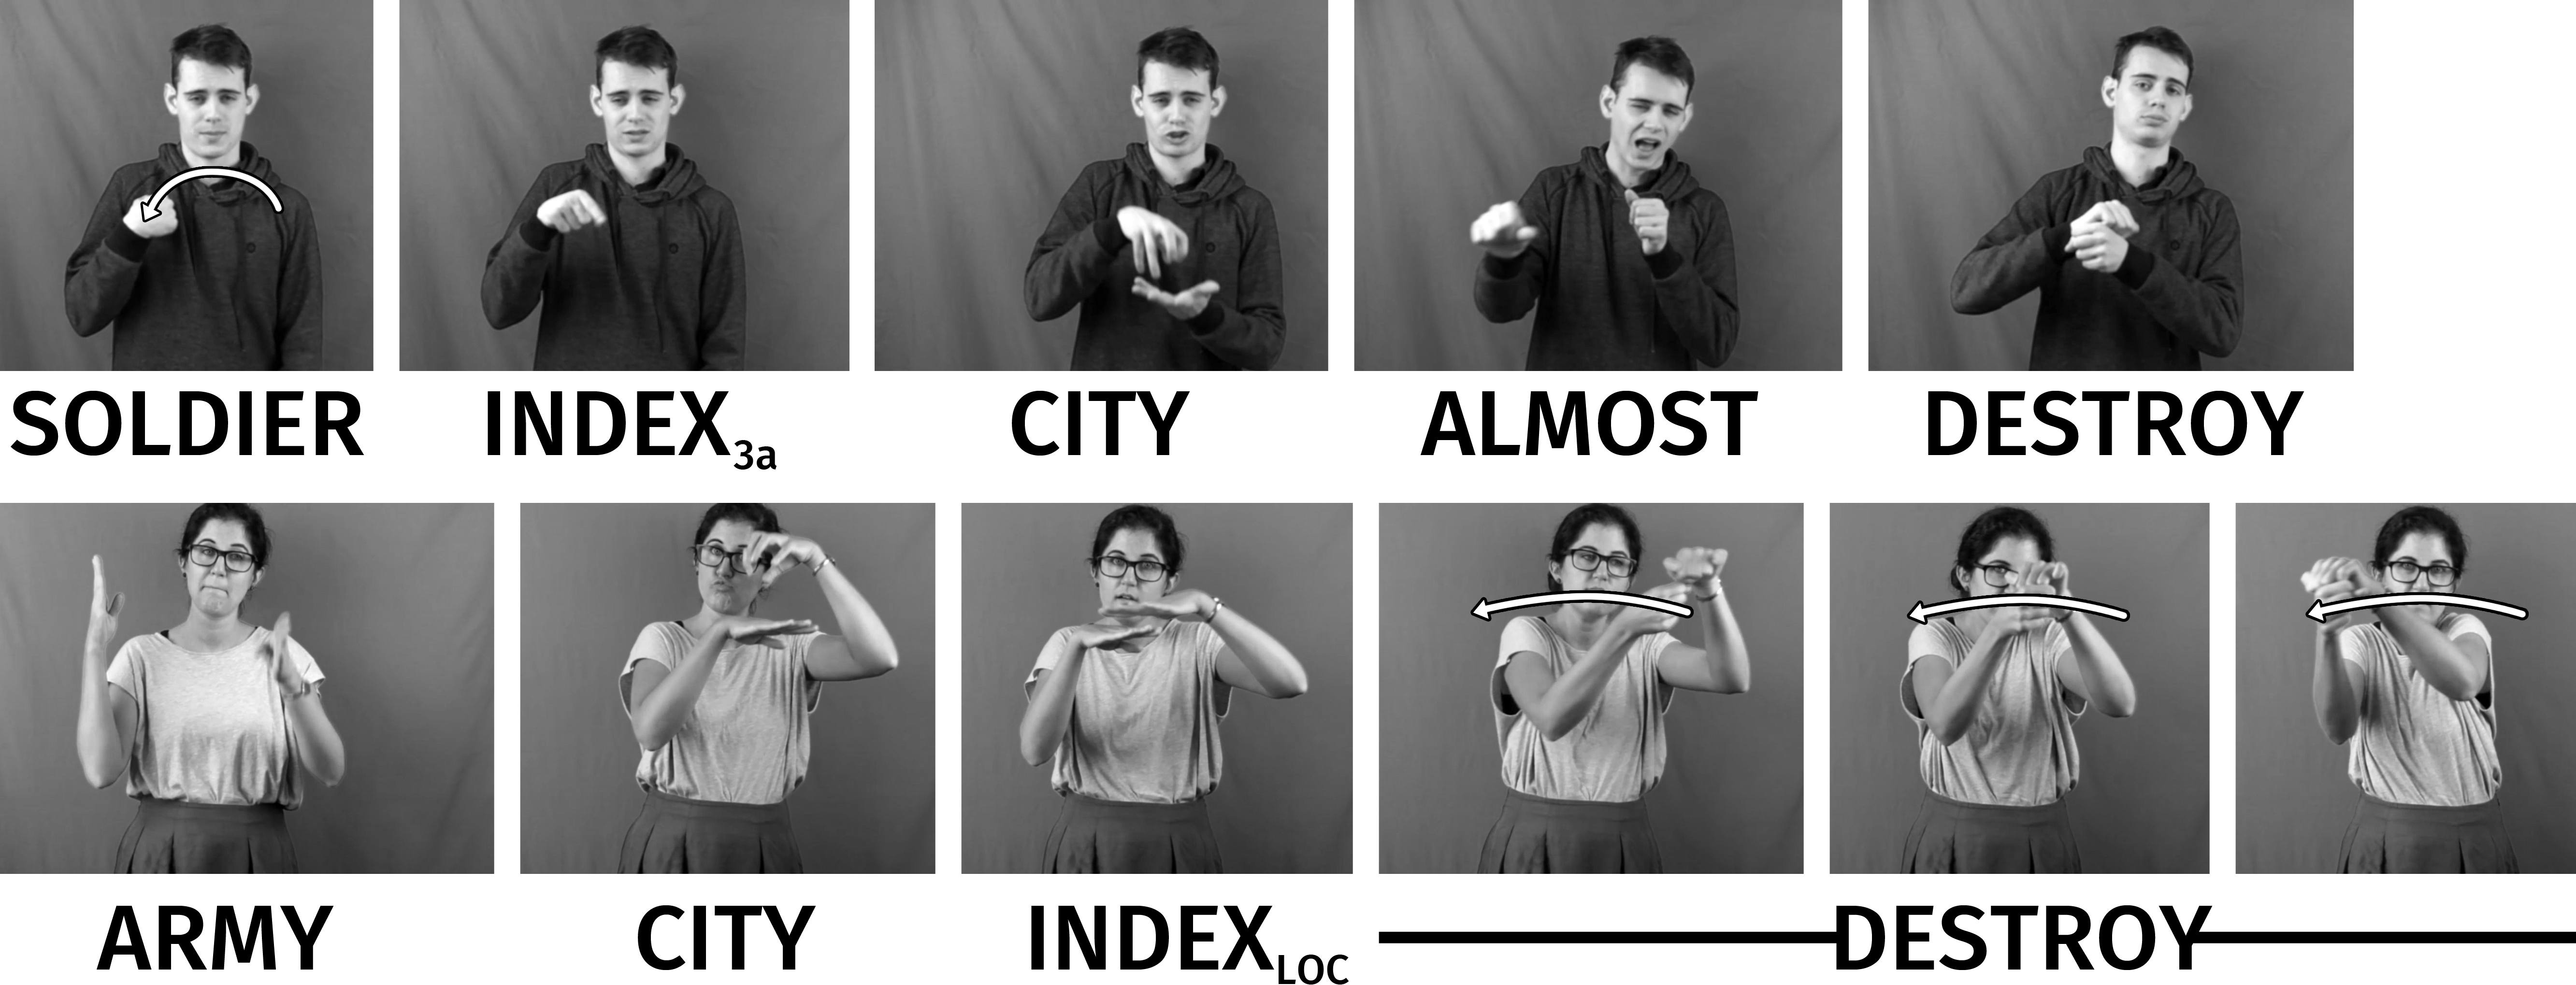
\includegraphics[width=1.0\textwidth]{completivetwosw.jpg}
	\caption{The two examples translate to \textit{The soldiers almost destroyed the city} (top) and \textit{The army completely destroyed the city} (bottom).}
	\label{fig:completivetwodgsexampletwo}
\end{figure}


\subsection{The situation in DGS}
As predicted, completive II is realized by modification of the verb. I will give two illustrative examples. The first example refers to a process in which all the sandwiches in the context are affected completely in that they are all eaten up. This is depicted in Figure \ref{labelfigure}. In this case, the hand shape and the way of execution of the verb sign \textit{eat} is altered in that the hand is open and the movement of the verb does not stop at the mouth, but proceeds to the chest (the left part of the image shows the actual example, the sign on the right is the normal sign \textsc{eat} not marked for aspect).

The second example refers to the destruction of a city and is depicted in Figure \ref{fig:completivetwodgsexampletwo}. The figure illustrates that the verbal sign \textsc{destroy} when not inflected for aspect refers to a point, as shown by the top example (`The soldiers almost destroyed the city'). When the object of the destruction, however, is completely affected, then this information is incorporated into the verbal sign. In this case (`The army completely destroyed the city', the second example in the figure), the verb is signed in the part of the signing space in which the city had been located previously by an locational index. It is not clear yet how completive II is realized with body-anchored verbs. I will leave this question open for future studies.



\begin{digression}{{A note on \textsc{finish}, \textsc{through} and perfective aspect}}{}
\noindent \label{exkursfertigdurch}A very similar, though distinct, meaning can be achieved by the perfective marker \textsc{finish} that marks a proposition as being without interior composition, as shown in (\ref{dgsfinish}). In this example, the reading of the book is also understood as being completed. It seems, however, that \textsc{finish} rather marks perfective aspect than completive aspect similar to what has been described for \is{American Sign Language}American Sign Language (e.g., \citealt{aarons1992clausal}) or \is{Italian Sign Language}Italian Sign Language (e.g., \citealt{zucchi2003}). However, it seems that the use of \textsc{finish} also seems to have a meaning of completive aspect in some sign languages (e.g., \citealt{meir1999aperfect} on \is{Israeli Sign Language}Israeli Sign Language). A similar meaning as the one contributed by the sign \textsc{finish} in DGS can be achieved by another clause-final element, that I glossed \textsc{through} in (\ref{dgsthrough}).


\begin{exe}
\ex\label{ex:perfectivea}\begin{xlist}
\ex{\textsc{paul book read finish}}     
\glt `Paul read the book.' \label{dgsfinish}
\ex{\textsc{paul book read through}}     
\glt `Paul read through the book.' \label{dgsthrough}
\end{xlist}
\end{exe}

\noindent The sign \textsc{through} is also described in \citet[259]{rathmann2005event}, however as a continuative marker. It is still unclear if the sign described by Rathmann and the sign discussed here are the same as Rathmann has no picture of it and does not describe how it is performed. It could, however, be that we are dealing with two different signs, as \textsc{through} in the example in (\ref{dgsthrough}) seems to have a different meaning than the one described by Rathmann. Thus more research is needed. Both signs, \textsc{finish} and \textsc{through}, are depicted in the following figure: \\

\begin{center}
	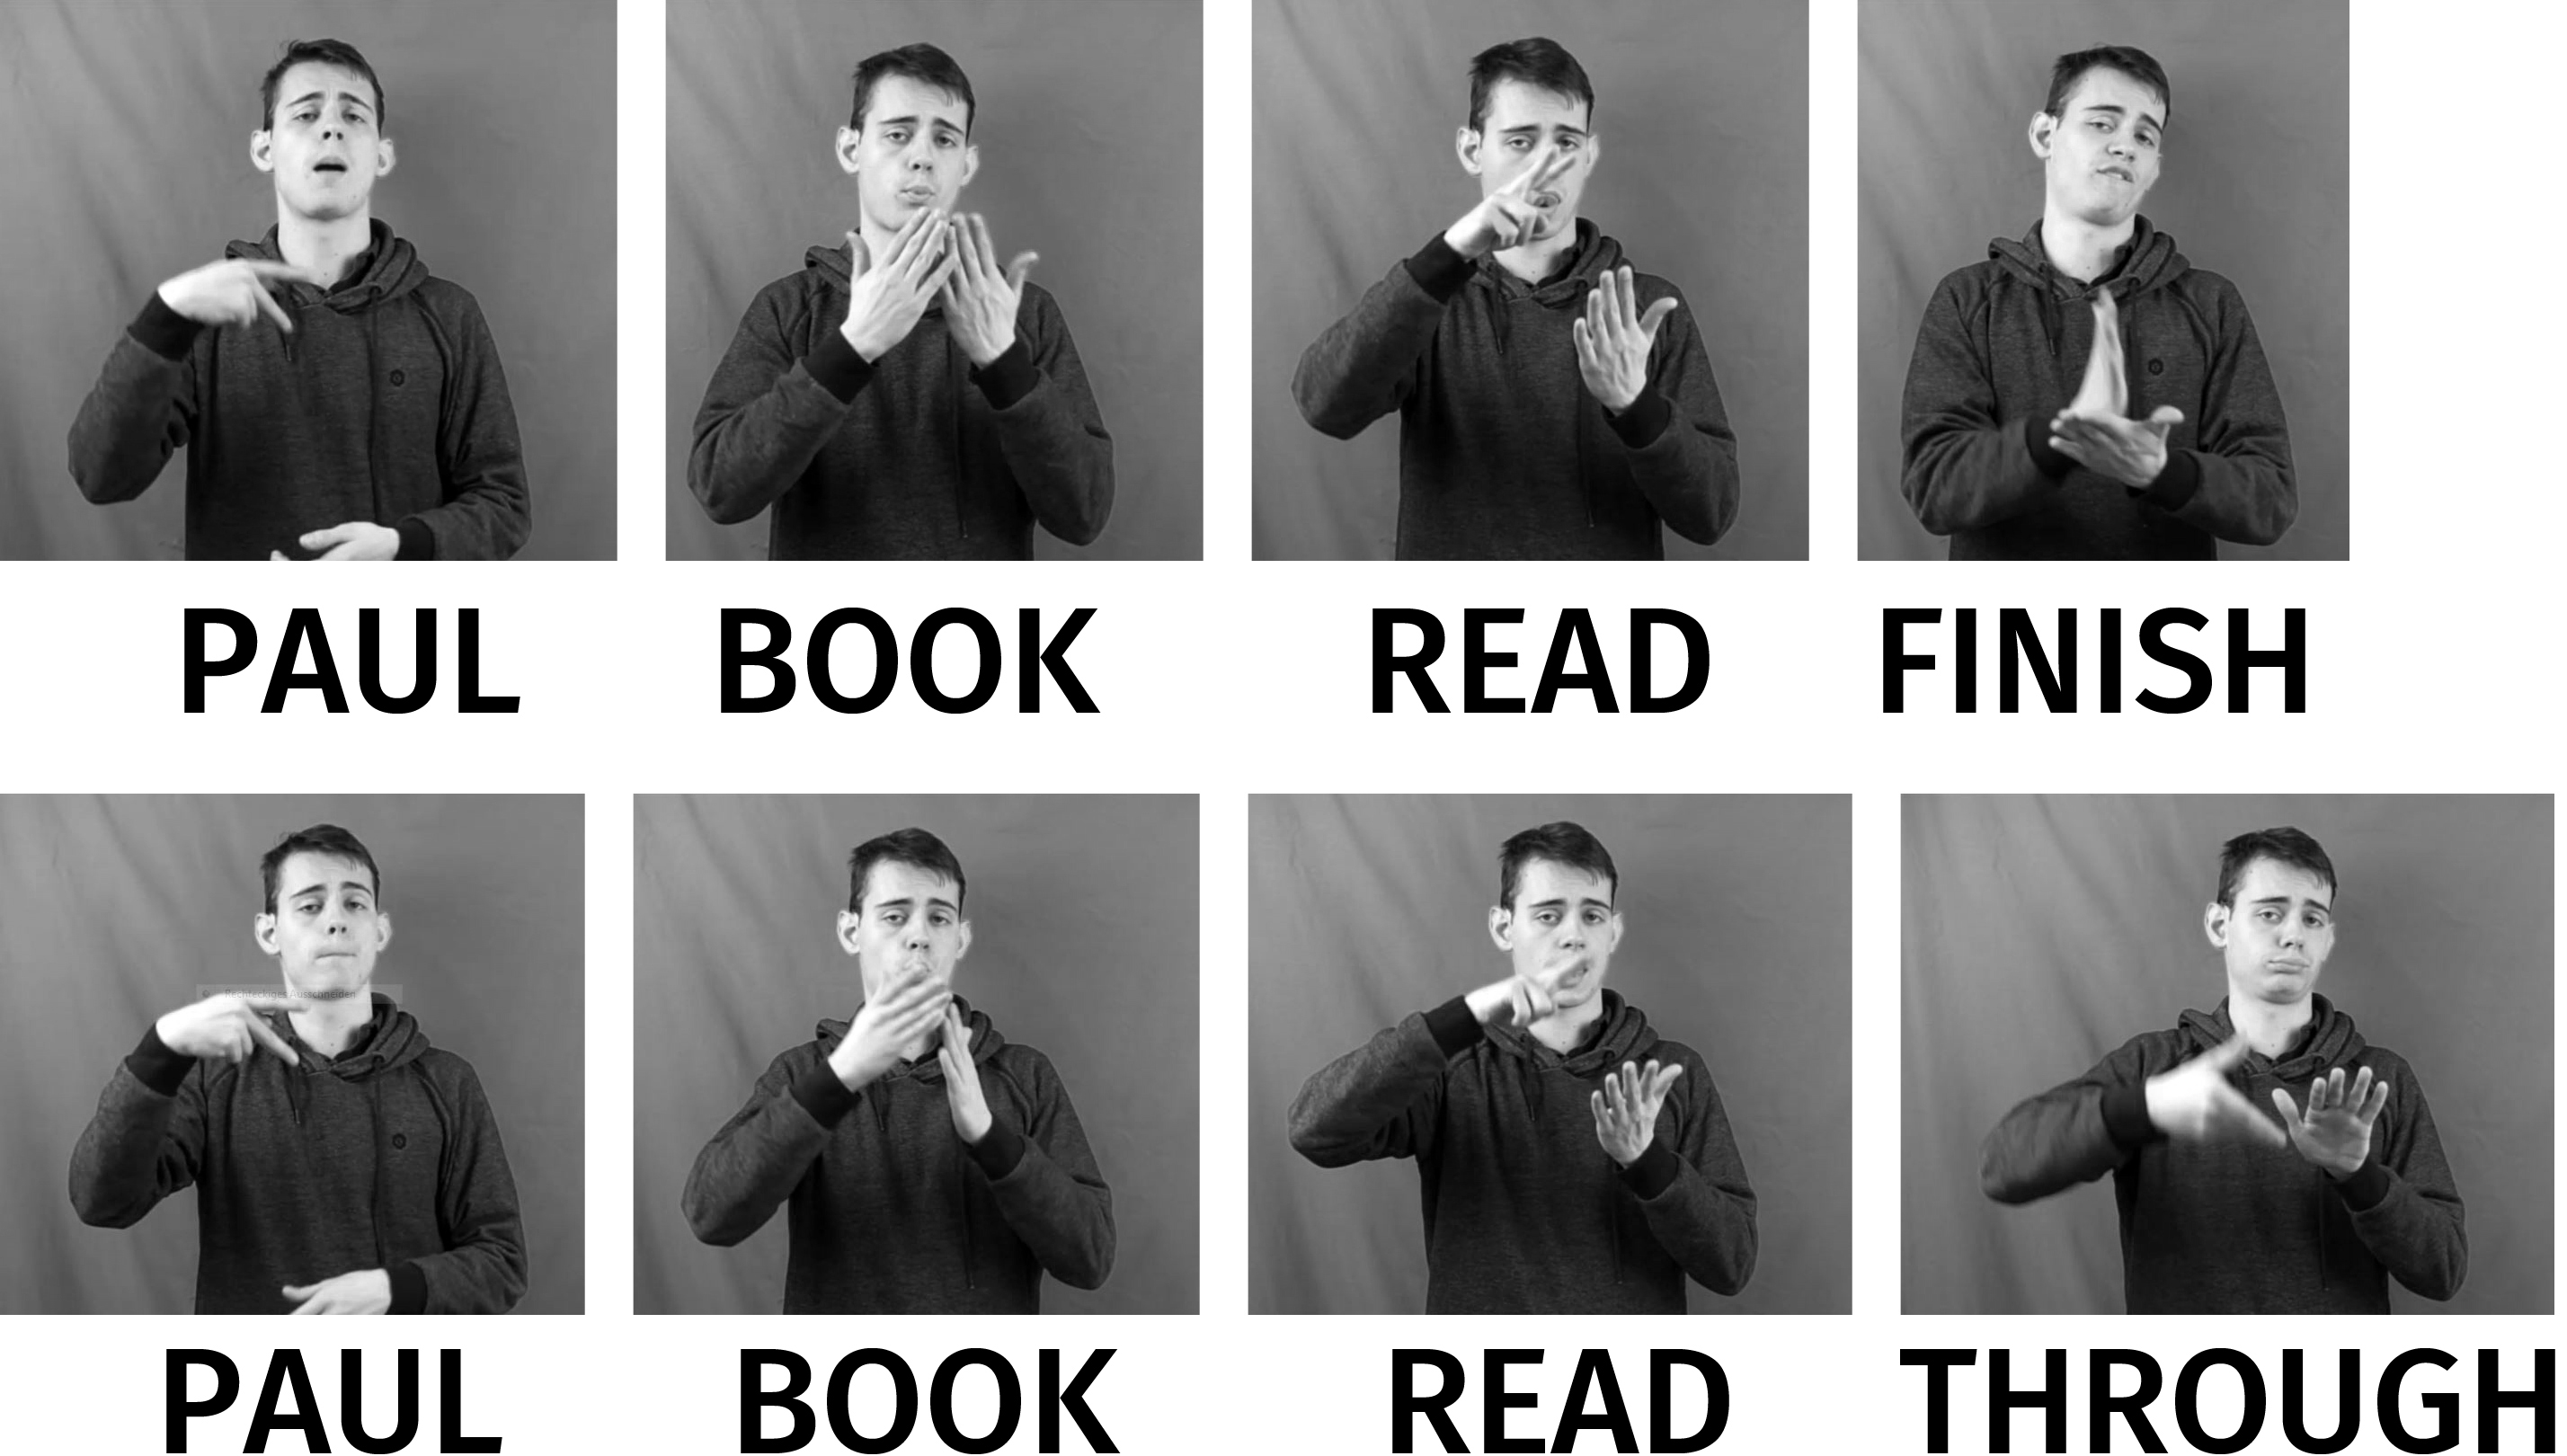
\includegraphics[width=0.5\textwidth]{fertigunddurchsw.jpg}
	\end{center}
	%\caption{Testcaption}
	%\label{fig:throughfinish}
\vspace{0.2cm}

\noindent Note that the perfective marker \textsc{finish} is usually described to be restricted to occurring in a clause-final position in the literature (e.g., \citealt[3]{pfau2004grammaticalization}; \citealt[261--262]{rathmann2005event}). However, I often found \textsc{finish} in a pre-verbal position. It is yet unclear if this leads to differences in meanings as has been described for \is{American Sign Language}American Sign Language (see \citealt{rathmann2005event}). It is also unclear how to model this syntactically. It may also turn out that \textsc{finish} is located in a small clause\is{small clause}.
%\end{theo}
\end{digression}



\is{completive aspect|(}

\section{Repetitive aspect II (\textit{again})}\label{repetitivetwo}\is{repetitive aspect II|(}
\subsection{General overview}
While repetitive aspect I refers to the iteration of an event on a single occasion (see Section \ref{repetitiveonesection} on page \pageref{repetitiveonesection}), repetitive II refers to the iteration of a process. In contrast to frequentative aspect which refers to several repetition (\textit{often}), repetitive aspect is about a single iteration (\textit{again}, \textit{once more}). 

\subsection{The situation in DGS}
It would be easy to imagine that repetitive aspect II finds its expression in repeating the verb sign: a plausible scenario would involve first signing the verb, making a short pause, and signing it again to indicate that the process repeated (the two processes would  then refer to one single event). However, this is not what we find. It is either manually indicated how often the process was repeated (e.g., twice) or the verb is repeated two times, but the manual adverb \textsc{again} is sandwiched in between the two verbs, as shown in (\ref{ggsrepetitivetwo}).


\begin{exe}
\ex {\textsc{paul door knock, again knock}}     
\glt `Paul knocks on the door again.' \label{ggsrepetitivetwo}
\end{exe}

\noindent As the example shows, there is a pause after the first instance of \textsc{knock} that leads to the impression that we are not dealing with some kind of grammaticalized sandwich structure, but rather with two clauses (\textit{Paul knocked at the door and then knocked again}). Therefore, I conclude, that repetitive aspect II is not grammaticalized in DGS. 
\is{repetitive aspect II|(}




\section{Frequentative aspect II (\textit{often})}\label{frequentatitivetwo}\is{frequentative aspect II|(}
\subsection{General overview}
As was noted in Section \ref{frequentative}, frequentative aspect I is expressed by using the (left-to-right concatenated) manual sign \textsc{often}. Examples for frequentative I are, for convenience, given in (\ref{ex:freqaspIa}) and (\ref{ex:freqaspIb}) again. In this case, the event of insulting occurs frequently, for example, every day. This means that the event occurs frequently on different occassions. 

\begin{exe}
\ex\begin{xlist} 
\ex[]{\textsc{paul pam maria often insult} 
\glt `Paul insults Maria often.' \label{ex:freqaspIa}}
\ex[*]{\textsc{paul pam maria insult often}
\glt `Paul insults Maria often.' \label{ex:freqaspIb}}
\end{xlist}
\end{exe} 

\noindent With frequentative II, the event also occurs frequently, but on one occasion. \citet[92]{cinque1999adverbs} illustrates this difference with Italian adverb \textit{spesso} that can occur in two different positions, as shown in (\ref{ex:cinquefreqa}) and (\ref{ex:cinquefreqb}). The two different positions can be easily identified by its relative position to \textit{già} `already' in the examples. 

\begin{exe}
\ex Italian \citep[92]{cinque1999adverbs}\begin{xlist} 
\ex {(Quando troviamo qualcosa) questa è \textit{spesso già} stata scoperta da qualcuno.} \\
`(When we find something) that has often already been discovered by someone.' \label{ex:cinquefreqa}
\ex {Questa proprietà è \textit{già} stata scoperta \textit{spesso}, negli ultimi cinquant'anni.} \\
`This property has already been discovered often, in the last fifty years.' \label{ex:cinquefreqb}
\end{xlist}
\end{exe} 


\noindent As the examples show, \textit{spesso} in its higher position, in (\ref{ex:cinquefreqa}), refers to different events that are viewed as completed. The lower one, in contrast, refers to a frequency in one time interval as in (\ref{ex:cinquefreqb}). Cinque assumes that there are not two different \textit{spesso}, but that they occupy two different (scope) positions in the clause. Note that both positions can be filled in one clause, as exemplified in (\ref{ex:cinquefreqc}), taken from \citet[92]{cinque1999adverbs}.

\begin{exe}

\ex Italian \citep[92]{cinque1999adverbs} \\ {Gianni saggiamente, \textit{spesso} esce con la stessa persona \textit{spesso}.} 
\glt `Gianni, wisely, often dates the same person often.' \label{ex:cinquefreqc}

\end{exe} 


\subsection{The situation in DGS}
\noindent In DGS, \textsc{often} cannot be used for expressing frequentative II. Instead, we find a \is{reduplication}reduplication of the verbal sign, as illustrated in (\ref{ex:freqaspIIa}). With this, DGS behaves similar to \is{American Sign Language}American Sign Language as described by \citet{klima1979signs,rathmann2005event}; see also \citet{pfausteinbwol2012tense} where this category has also been labeled `iterative aspect'.\is{iterative aspect}

Note that the reduplication in (\ref{ex:freqaspIIa}) does not consist of a single repetition of the sign, but of several repetitions, sometimes with short pauses between the repetitions \citep[163]{papaspyrou2008grammatik}. Additionally, \textsc{often} and the reduplication of the verb sign can easily combine into one sentence, as shown in (\ref{ex:freqaspIIb}).


\begin{exe}
\ex\label{frequecsaca}\begin{xlist} 
\ex {\textsc{paul pam maria insult+++}} 
\glt `Paul insults Maria often ($=$ many times on a single occasion).' \label{ex:freqaspIIa}
\ex {\textsc{paul pam maria often insult+++}} 
\glt `Paul often insults Maria often.' \label{ex:freqaspIIb}
\end{xlist}
\end{exe} 

\noindent Similar observations, namely that frequentative II involves the fast \is{reduplication}reduplication of the verb root, have been made for many sign languages (e.g., \citealt{bergmandahl1994, sutton1999linguistics, meir2007language} and seems to be a cross-linguistically stable pattern \citep[227]{signgram2017}.\footnote{ It could turn out in the end that at least some instances of what is often labeled `habitual aspect' in the literature and frequentative II are one and the same category. }

\is{frequentative aspect II|)}

\section{Summary and conclusion}
The discussion in this chapter has shown that the inner aspects taking scope below VoiceP indeed find their expression by manipulating the movement path of the verb sign. Additionally, I have argued that what is usually labeled habitual aspect in the sign language literature, a category expressed by \is{lower layering}lower layering, also belongs to the inner aspects. Evidence for this claim came from the fact that it is not possible to use this habitual aspect II with scope above modal verbs. A similar claim was made for the so called `durative'. 

It is still unclear if these observations map one-to-one to other sign languages. However, similar patterns are attested even in spoken languages. In German, for example, frequentative I and frequentative II is expressed by the adverb \textit{oft} `often'. It is, however, also possible to add a bound morpheme to the verb to express frequentative II. The verb \textit{tropfen} `to drip', for example, can be transformed into \textit{tröpfeln} which expresses the existence of many drips at a single event time (therefore it is not possible to say *\textit{Der Wasserhahn wird ein mal tröpfeln} `The tap will drip one time.').\footnote{ Note that the suffix -\textit{eln} not only leads to an iterative, but also to a diminutive reading. Additionally, other meanings like `low intensity' can be contributed by the suffix (cf. \citealt{weidhaasschmid2015diminutiv}). The iterative meaning is, however, clearly added if the suffix is attached to an already existing verb. In other cases, when the suffix is used to derive a verb from an adjective, for example, sometimes only diminutive readings survive, as in \textit{krank} `sick' $\rightarrow$ \textit{kränk-eln}.} While using the adverb \textit{oft} can be equated with using a manual sign, the use of the bound morpheme can be equated with \is{lower layering}lower layering.

\begin{figure}[bt]
\centering
	\includegraphics[width=1.00\textwidth]{lowerlayeringsw.jpg}
	\caption{A comparison of outer and inner aspects. The comparison of continuative aspect I\is{continuative aspect I} (A) and continuative aspect II\is{continuative aspect II} (B), celerative aspect I\is{celerative aspect I} (C) and celerative aspect II\is{celerative aspect II} (D), completive aspect I\is{completive aspect I} (E) and completive aspect II\is{completive aspect II} (F), and frequentative aspect I\is{frequentative aspect I} (G) and frequentative aspect II\is{frequentative aspect II} (H) reveals that the inner aspects are formed by manipulating the movement path of the verb sign.}
	\label{fig:lowerlayering}
\end{figure}

Figure \ref{fig:lowerlayering} summarizes the findings by comparing the expression of the outer aspects (labeled with the number I by Cinque) and the inner aspects (labeled with the number II by Cinque). The figure shows examples of continuative aspect I\is{continuative aspect I} and II (A and B), \is{celerative aspect I}celerative aspect I and II (C and D), \is{completive aspect I}\is{completive aspect II}completive aspect I and II (E and F), as well as \is{frequentative aspect I}frequentative aspect I and II (G and H). Comparing the expressions of the IP-internal outer aspects with the VoiceP-internal inner aspects shows that each outer aspect is expressed by one separate sign (with the exception of completive I), while the inner aspects are formed as predicted by the VoiceP-internal modulation hypothesis, namely by manipulating the movement path of the verb sign.



%Regarding the inner aspects I have argued that they find their expression via lower layering, i.e., by manipulating the movement path of the verb sign. The two probably most controversial claims in this area were that what is usually called `habitual aspect' in the sign language literature is actually an instantiation of a lower VoiceP-internal category and that what is usually labeled \index{durative aspect}`durative aspect' is actually an instance of celerative II\index{celerative aspect II}. For the other inner aspects discussed by Cinque (1999, 2006) I have shown that they either find their expression by lower layering (continuative II\index{continuative aspect II}, celerative II\index{celerative aspect II}, completive II\index{completive aspect II}, frequentative\index{frequentative aspect II} II) or have no grammaticalized expression in DGS at all (inceptive \index{inceptive aspect II}II, repetitive\index{repetitive aspect II} II). 


%It is still unclear if these observations map one-to-one to other sign languages. However, similar patterns are attested even in spoken languages. In German, for example, frequentative I and frequentative II is expressed by the adverb \textit{oft} `often'. It is, however, also possible to add a bound morpheme to the verb to express frequentative II. The verb \textit{tropfen} `to drip', for example, can be transformed into \textit{tr\"opfeln} which expresses the existence of many drips at a single event time. While using the adverb \textit{oft} can be equated with using a manual sign, the use of the bound morpheme can be equated with \is{lower layering}lower layering. 

%With this, I end the discussion of the Cinquean categories. I will now discuss the behavior of the direct object in DGS and thus descend the tree even further, namely to the position in the tree in which the syntactic object is base-generated. In the following sections I will discuss object shift and differential object marking in DGS. 


\chapter{Conclusions}\label{chapterconclusions}
In this last chapter I will briefly review the main findings of the book. As each chapter ended with a brief summary, I will not summarize these findings here again. Instead, this chapter tries to bring together the individual insights in discussing the main hypotheses which guided the book:


\begin{itemize}[itemsep=0pt]
	\item The \is{bodily-mapping hypothesis}bodily-mapping hypothesis by \citet{bross2017scope}: clausal categories with higher scope are expressed by articulators which are higher, or at least have the same height, than categories with lower scope (i.\,e., descending the scopal hierarchy of the clause equates to descending the signer's body).
	\item Categories below tense are expressed by manual concatenation -- starting with a left-to-right-concatenation strategy and finally switching to concatenation from right to left.
	\item The split between categories above tense being expressed non-manually and categories below tense being produced by manual signs is a general split between not-at-issue and at-issue meanings.
	\item The VoiceP-internal modulation hypothesis: categories below the VoiceP level are expressed by manipulating the movement path of the verb sign (lower layering)\is{lower layering}.
\end{itemize}

\noindent While the bodily-mapping hypothesis was put to test throughout the book, the question of whether the categories below tense are, in contrast to the categories above tense, indeed produced manually was discussed in Chapter \ref{ipsystem}. The same chapter was concerned with the at-issue/not-at-issue divide. Lastly, the VoiceP-internal modulation hypothesis was discussed in Chapter \ref{insidevp}. In the following, I will briefly review the main findings of the book regarding the main hypotheses.

\section{The bodily-mapping hypothesis}
\is{bodily-mapping hypothesis|(}
The main claim of the bodily-mapping hypothesis is that the expression of scope is systematically, or even iconically\is{iconicity}, mapped onto the body in sign languages. The higher the scope of an operator is, the higher the articulator used for its expression will be. It should thus be impossible that a low category, for example, root modality, finds its expression with the eyebrows in a sign language, while a high category, let's say epistemic modality, is expressed manually only. However, it is clear that it should not be ruled out in general that a language may employ a manual strategy for expressing a high category. Then, however, a lower category should not switch back to a higher articulator. 

\begin{figure}[bt]
\centering
	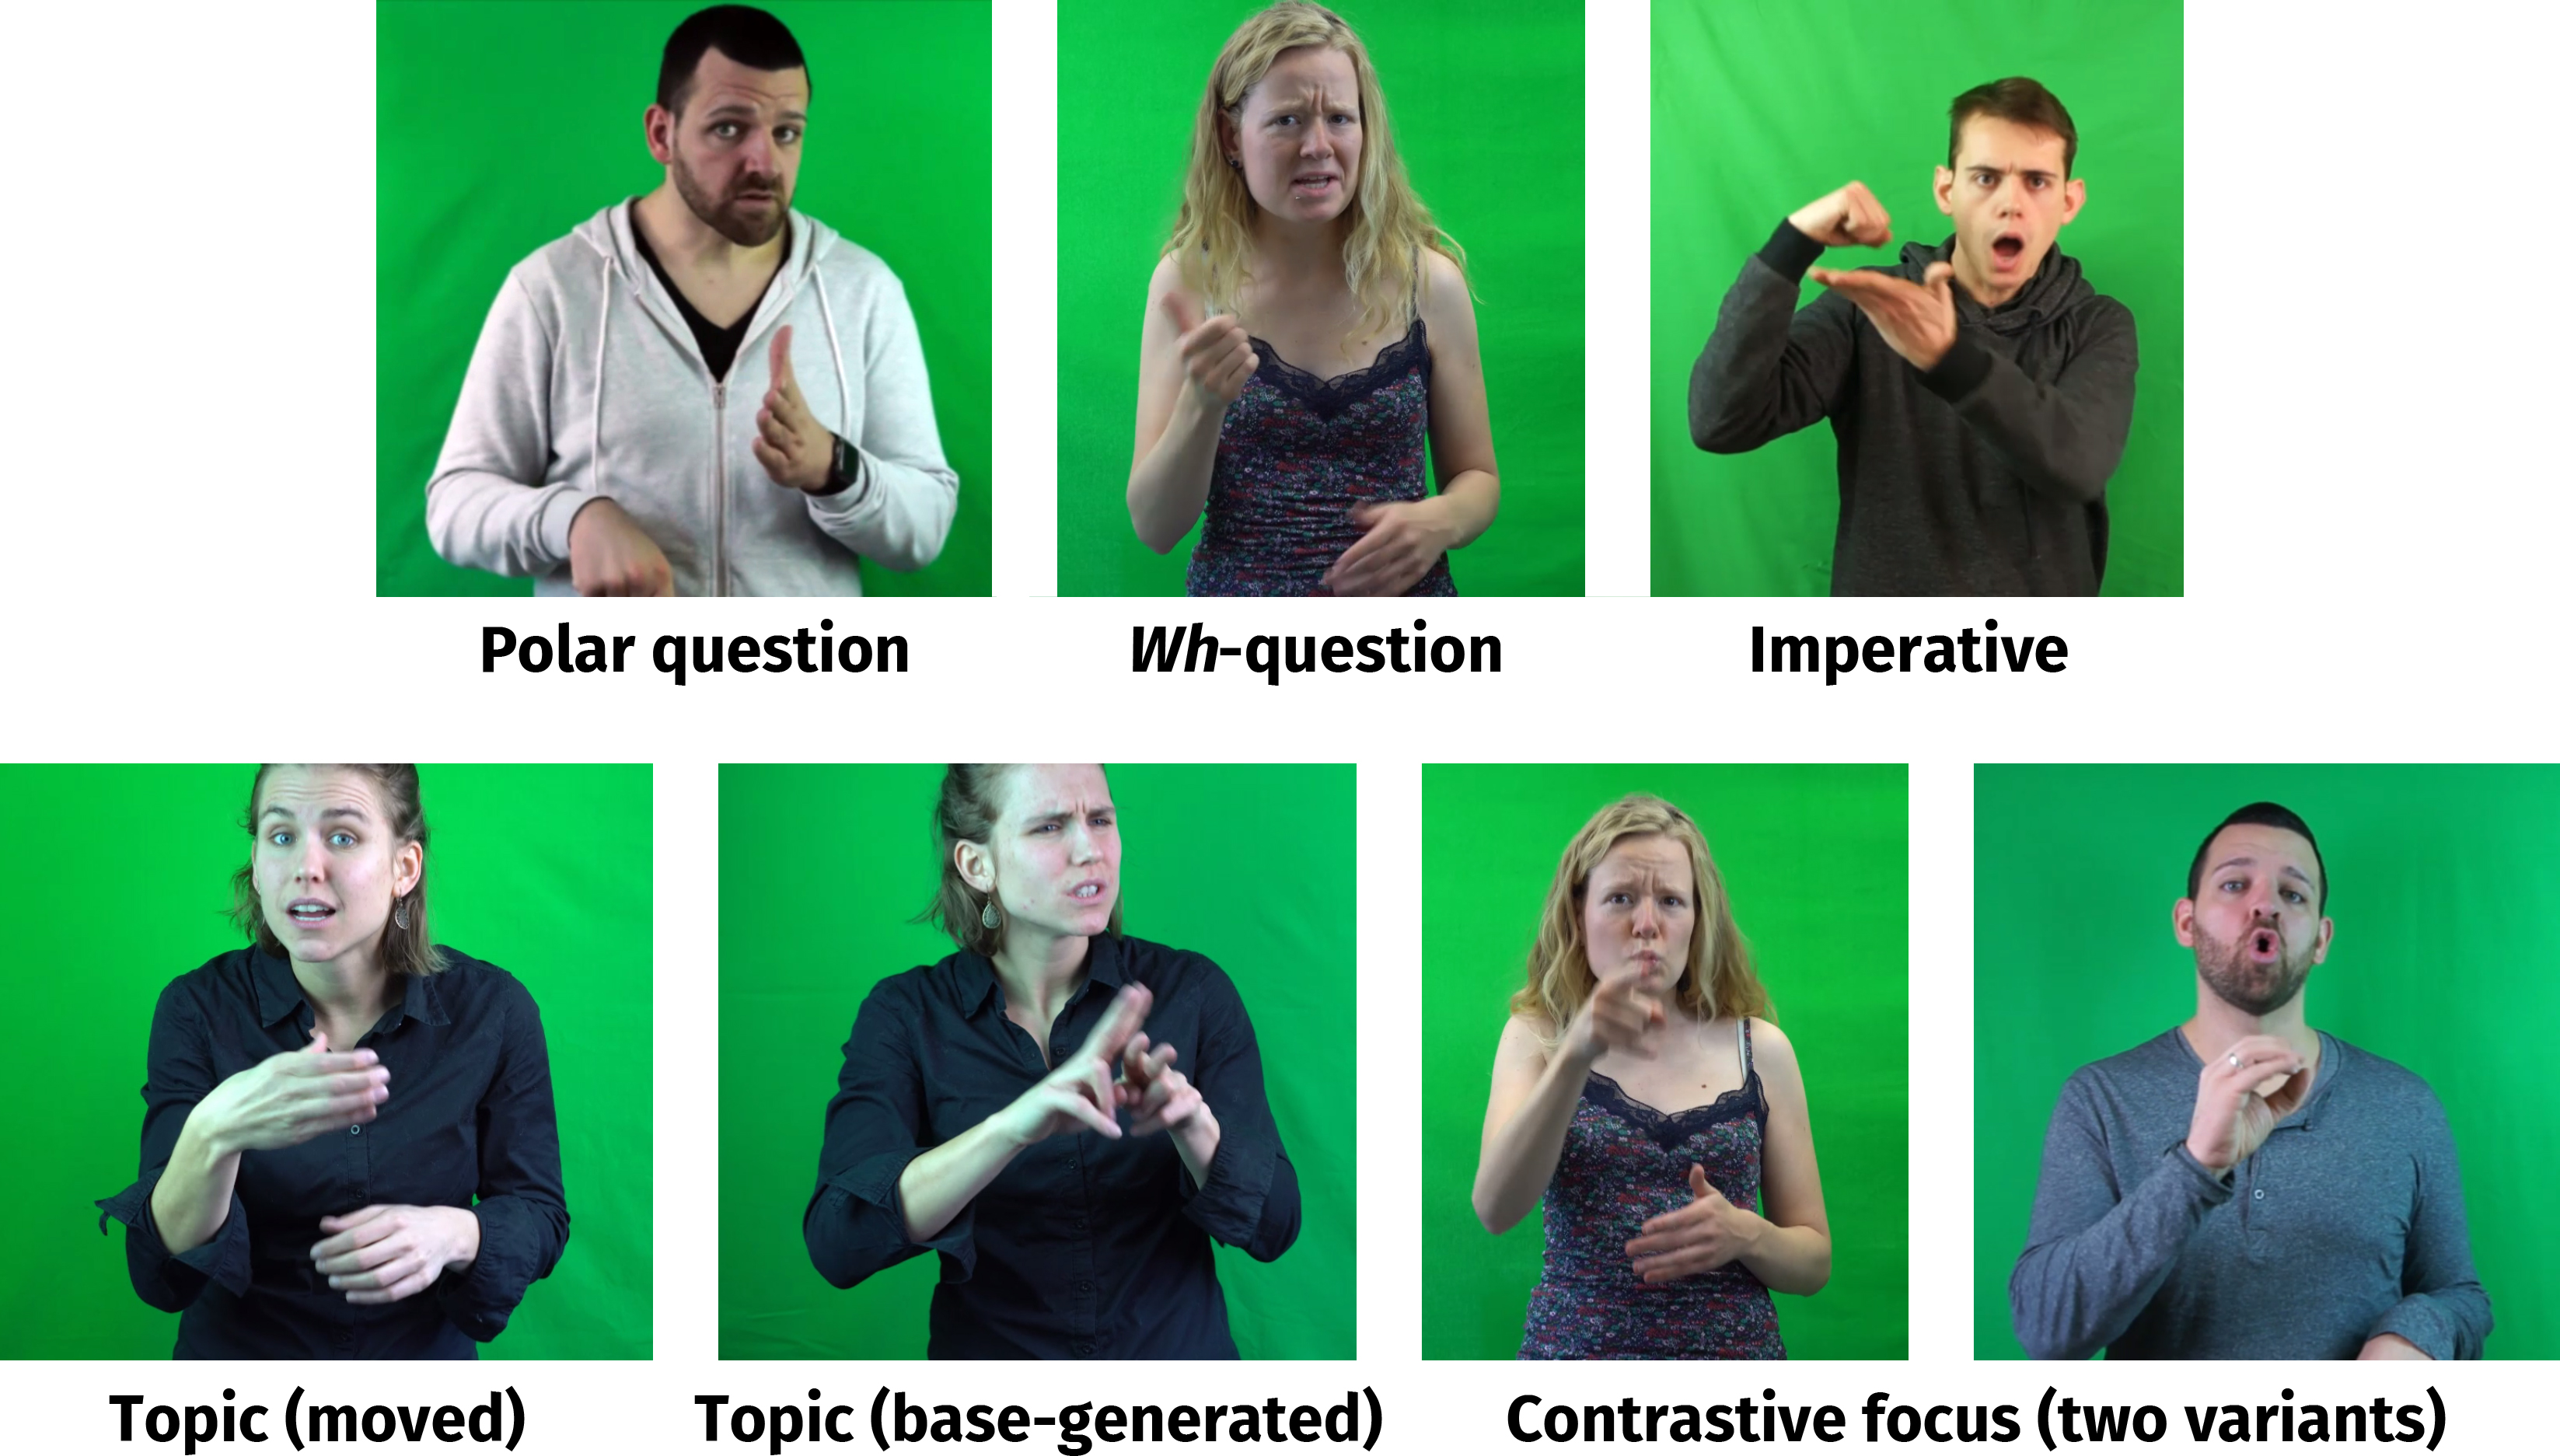
\includegraphics[width=1.0\textwidth]{uebersicht.jpg}
	\caption{All higher CP categories are expressed non-manually with the highest possible articulator, i.\,e., the eyebrows, sometimes together with other non-manuals. The upper row shows speech-act markings, the bottom row topic and focus marking (the expression of contrastive focus is subject to dialectal variation).}
	\label{highercpcategories}
\end{figure}

Indeed all categories above tense were found to be expressed non-manually only or by a combination of a manual sign plus a non-manual marker. All higher CP categories are expressed non-manually only in DGS: sentence types are encoded by using the eyebrows in DGS. While the same is true for moved and base-generated topics, focus marking involves several articulators including the head and, crucially, the eyes/eyebrows. Although contrastive focus was found to be subject to dialectal variation, both variants make use of the eyebrows. I have summarized the main non-manual markers used to express the higher CP categories in Figure \ref{highercpcategories}.

Additionally, all remaining categories above tense included in Cinque's system were found to be expressed either non-manually only or by a combination of non-manuals and manual signs. Two problematic cases were what Cinque called `irrealis mood'\is{irrealis mood} and `alethic modality' as both are categories which he puts below tense, but find non-manual expression with the upper face. In the case of irrealis mood (Section \ref{perhapsmoodirrealis}) I have argued, following \citet{nordstrom2010modality} and \citet{zyman2012two}, that irrealis mood and epistemic modality have the same distribution and both are structurally higher than tense. In the case of alethic modality\is{alethic modality} (Section \ref{alethicmodal}), I have argued, following \citet{palmer1986mood}, \citet{nuyts2000epistemic}, and \citet{von2006modality}, that it probably does not constitute a category on its own, but coincides with epistemic modality -- or, alternatively, that it is located above tense. This is in line with the finding that, similar to what has been described for spoken languages, there seems to be no difference in the expression of alethic and epistemic modality in DGS.

\begin{figure}[bt]
\centering
	\includegraphics[width=1.0\textwidth]{uebersicht2.jpg}
	\caption{All Cinquean categories above tense find non-manual expression with the eyebrows and the eyes, sometimes together with other non-manuals.}
	\label{lowercpcategories}
\end{figure}

The higher Cinquean categories are expressed with the eyebrows or the eyes. Descending the hierarchy, one finds that scalarity (Section \ref{scalarity}) is produced by inflating or sucking in the cheeks. While DGS has no grammaticalized tense system, other sign languages which do have such a system use the shoulders to express tense (Section \ref{tense}). Both observations are in line with the idea of the bodily-mapping hypothesis. The non-manual markers used to express the higher categories in Cinque's system are depicted in Figure \ref{lowercpcategories}.

Taken together, all categories above tense are expressed non-manually. No category was found to take higher scope than another category, in which the former is expressed with a lower articulator than the latter. To the contrary, while most CP categories are expressed using the eyebrows, the lowest CP category, scalarity, is expressed by using a lower articulator, namely the cheeks. While the next lower category, tense, is not grammaticalized in DGS, temporal adverbs as well as all other IP- and VoiceP-internal categories are expressed with the lowest possible articulator, namely the hands. Thus, scope-taking in the clausal spine starts out with the eyebrows, descending the spine, scope-taking moves along the body on a vertical axis, through the cheeks (and the shoulders in some sign languages), then reaching the hands and finally switching to a strategy that incorporates categories into the movement path of manual signs. That neighboring categories are expressed by similar strategies is furthermore in line with the principle of analogical designation\is{analogical designation} stating that syntactic proximity is mirrored by phonological similarity. 

\is{bodily-mapping hypothesis|)}


\section{Concatenation strategies in DGS}\label{concatenatiostrategies}
While I claim that the bodily-mapping hypothesis may turn out to hold true in all sign languages, the question at which point in the clausal spine a language employs a left-to-right-concatenation or a right-to-left-concatenation strategy is thought to be subject to cross-linguistic variation -- just as in spoken languages. For (Southern) DGS it turned out that all categories below tense, but above the VoiceP level, find manual expression (without any layering). However, there were three exceptions to this generalization. In Section \ref{justjust} I described that the sign \textsc{just}, an instantiation of retrospective aspect\is{retrospective aspect}, is accompanied by a non-manual marker produced with the tongue. This deviation was explained by the assumption that this sign is always accompanied by the evaluation of a time interval as being little. Evidence for this claim comes from the fact that the intensity of the non-manuals can vary -- as a function how little the time interval is evaluated to be. In Section \ref{habitualaspect} I discussed that habitual aspect can be expressed through a manipulation of the movement path of the verb sign and in Section \ref{durativeaspect} I have shown that the same is true for durative aspect. In the case of habitual aspect expressed via \is{lower layering}lower layering I have shown that it should be taken as an instance of a lower scoping category as it cannot take scope above root modality (see Section \ref{habitualtwo})\is{habitual aspect}. A similar claim was made for durative aspect.

Taken together, I have argued that all IP-internal categories are expressed manually. Scope-taking generally proceeds from left to right as the natural landing site of the adverbs is to the left of the VP. This claim was supported by the fact that when two manual adverbs combine, the one with higher scope always precedes the one with lower scope. In contrast to what was claimed in \citet{bross2017scope}, the turning point from left-to-right to right-to-left concatenation was not found at root modality, but only with the lowest IP-internal category of manner adverbs (e.\,g., \textit{well}): the natural landing site of these adverbs is a post-verbal position. While modals show much more positional freedom (on the surface), the position of adverbs was found to be more restricted. Nevertheless, the combination of several modal verbs resulted in the predicted order (volitional modals, for example, have to precede root modals). 

\section{The at-issue/not-at-issue divide}\is{at-issue meaning|(}
In Section \ref{atnotissue} I have argued, following an idea by \citet{bross2017scope}, that the split between categories finding non-manual and categories finding manual expression is not only a split between the categories above and those below tense, but also a semantic split as the categories above tense contribute not-at-issue meaning while the categories below tense have a truth-conditional meaning contribution. While more empirical work has to be done in this domain, the presented results indicate that non-manual marking indeed generally contributes not-at-issue information. 

While this is clearly true for the higher CP categories which find non-manual expression only (e.\,g., speech-act markings), the picture with regard to the categories which can either be expressed non-manually only or by a combination of non-manual and manual expression (e.\,g., mirative marking) is more complex. In contrast to spoken English (or German), the manually signed adverbs were rated as contributing at-issue information by the signers I consulted. On the whole, the hypothesis that non-manuals express not-at-issue and manuals express at-issue meaning seems to be true. %The question whether higher (speaker-oriented) adverbs 



\is{at-issue meaning|)}


\section{The VoiceP-internal modulation hypothesis}
\is{VoiceP-internal modulation hypothesis|(}\is{lower layering|(}
In the previous chapter I have argued that all Cinquean categories below VoiceP find expression by lower layering, i.\,e., by manipulating the movement path of the verb sign. Problematic cases were what is called `habitual aspect' and `durative aspect' in the literature as both should belong to higher, IP-internal categories, but find expression by \is{lower layering}lower layering. In both cases, I have argued that these categories are indeed located below VoiceP (see also Section \ref{concatenatiostrategies} in this chapter). 


Taken together, I have found no counter-evidence for the idea that VoiceP-internal categories are expressed by single (manual) signs or even by higher articulators such as the eyebrows. Instead, all categories were found to be either expressed by lower layering\is{lower layering} (continuative II\is{continuative aspect II}, \is{celerative aspect II}celerative II, completive II, frequentative II) or have no grammaticalized expression in DGS at all (inceptive II\is{inceptive aspect II}, \is{repetitive aspect II}repetitive II). 


That the inner aspects are expressed by modulating the movement path of the verb sign is, in a sense, a case of iconicity and fits in well will the idea that there is some direct mapping of event structure and the morphological shape of a (manual) sign in sign languages in general, a proposal which has been called the \is{event visibility hypothesis}event visibility hypothesis (e.\,g., \citealt{wilbur2004event, wilbur2008complex, grose2007events}).



\is{VoiceP-internal modulation hypothesis|)}
\is{lower layering|)}


\section{Final remarks}
%It has been fun, but now I'm done!
%Ich hoffe, ein neues, fruchtbares Forschungsfeld eröffnet zu haben, das auch noch easy zu testen ist :)
I hope that this book has shown that the Cartography of sign languages is a fruitful and easy-to-conduct research approach. While many of the results presented in the previous chapters certainly need further investigation, I am confident that the general patterns will reproduce -- also in other sign languages. 




%%%%%%%%%%%%%%%%%%%%%%%%%%%%%%%%%%%%%%%%%%%%%%%%%%%% 
%%%             Backmatter                       %%% 
%%%%%%%%%%%%%%%%%%%%%%%%%%%%%%%%%%%%%%%%%%%%%%%%%%%%

% \is{some term| see {some other term}}
\il{some language| see {some other language}}
\issa{some term with pages}{some other term also of interest}
\ilsa{some language with pages}{some other lect also of interest} 
% There is normally no need to change the backmatter section


{\sloppy%There is normally no need to change this file
\sloppy
\backmatter
\phantomsection%this allows hyperlink in ToC to work
{\sloppy\printbibliography[heading=references]
\cleardoublepage

\phantomsection 
\addcontentsline{toc}{chapter}{Index} 
\addcontentsline{toc}{section}{Name Index}
\ohead{\lsNameIndexTitle} 
\printindex 
\cleardoublepage
  
%\phantomsection 
%\addcontentsline{toc}{section}{Language Index}
%\ohead{\lsLanguageIndexTitle} 
%\printindex[lan] 
%\cleardoublepage
  
\phantomsection 
\addcontentsline{toc}{section}{Subject Index}
\ohead{\lsSubjectIndexTitle} 
\printindex[sbj]
\ohead{} 
}
\end{document}
